\documentclass[twoside]{book}

% Packages required by doxygen
\usepackage{fixltx2e}
\usepackage{calc}
\usepackage{doxygen}
\usepackage[export]{adjustbox} % also loads graphicx
\usepackage{graphicx}
\usepackage[utf8]{inputenc}
\usepackage{makeidx}
\usepackage{multicol}
\usepackage{multirow}
\PassOptionsToPackage{warn}{textcomp}
\usepackage{textcomp}
\usepackage[nointegrals]{wasysym}
\usepackage[table]{xcolor}

% Font selection
\usepackage[T1]{fontenc}
\usepackage[scaled=.90]{helvet}
\usepackage{courier}
\usepackage{amssymb}
\usepackage{sectsty}
\renewcommand{\familydefault}{\sfdefault}
\allsectionsfont{%
  \fontseries{bc}\selectfont%
  \color{darkgray}%
}
\renewcommand{\DoxyLabelFont}{%
  \fontseries{bc}\selectfont%
  \color{darkgray}%
}
\newcommand{\+}{\discretionary{\mbox{\scriptsize$\hookleftarrow$}}{}{}}

% Page & text layout
\usepackage{geometry}
\geometry{%
  a4paper,%
  top=2.5cm,%
  bottom=2.5cm,%
  left=2.5cm,%
  right=2.5cm%
}
\tolerance=750
\hfuzz=15pt
\hbadness=750
\setlength{\emergencystretch}{15pt}
\setlength{\parindent}{0cm}
\setlength{\parskip}{3ex plus 2ex minus 2ex}
\makeatletter
\renewcommand{\paragraph}{%
  \@startsection{paragraph}{4}{0ex}{-1.0ex}{1.0ex}{%
    \normalfont\normalsize\bfseries\SS@parafont%
  }%
}
\renewcommand{\subparagraph}{%
  \@startsection{subparagraph}{5}{0ex}{-1.0ex}{1.0ex}{%
    \normalfont\normalsize\bfseries\SS@subparafont%
  }%
}
\makeatother

% Headers & footers
\usepackage{fancyhdr}
\pagestyle{fancyplain}
\fancyhead[LE]{\fancyplain{}{\bfseries\thepage}}
\fancyhead[CE]{\fancyplain{}{}}
\fancyhead[RE]{\fancyplain{}{\bfseries\leftmark}}
\fancyhead[LO]{\fancyplain{}{\bfseries\rightmark}}
\fancyhead[CO]{\fancyplain{}{}}
\fancyhead[RO]{\fancyplain{}{\bfseries\thepage}}
\fancyfoot[LE]{\fancyplain{}{}}
\fancyfoot[CE]{\fancyplain{}{}}
\fancyfoot[RE]{\fancyplain{}{\bfseries\scriptsize Generated by Doxygen }}
\fancyfoot[LO]{\fancyplain{}{\bfseries\scriptsize Generated by Doxygen }}
\fancyfoot[CO]{\fancyplain{}{}}
\fancyfoot[RO]{\fancyplain{}{}}
\renewcommand{\footrulewidth}{0.4pt}
\renewcommand{\chaptermark}[1]{%
  \markboth{#1}{}%
}
\renewcommand{\sectionmark}[1]{%
  \markright{\thesection\ #1}%
}

% Indices & bibliography
\usepackage{natbib}
\usepackage[titles]{tocloft}
\setcounter{tocdepth}{3}
\setcounter{secnumdepth}{5}
\makeindex

% Custom commands
\newcommand{\clearemptydoublepage}{%
  \newpage{\pagestyle{empty}\cleardoublepage}%
}

\usepackage{caption}
\captionsetup{labelsep=space,justification=centering,font={bf},singlelinecheck=off,skip=4pt,position=top}

%===== C O N T E N T S =====

\begin{document}

% Titlepage & ToC
\pagenumbering{alph}
\begin{titlepage}
\vspace*{7cm}
\begin{center}%
{\Large Vex Team A \\[1ex]\large 1.\+0.\+2 }\\
\vspace*{1cm}
{\large Generated by Doxygen 1.8.13}\\
\end{center}
\end{titlepage}
\clearemptydoublepage
\pagenumbering{roman}
\tableofcontents
\clearemptydoublepage
\pagenumbering{arabic}

%--- Begin generated contents ---
\chapter{In\+The\+ZoneA}
\label{md__r_e_a_d_m_e}
Team A code for In The Zone 
\chapter{Namespace Index}
\section{Namespace List}
Here is a list of all namespaces with brief descriptions\+:\begin{DoxyCompactList}
\item\contentsline{section}{\hyperlink{namespacetest_math}{test\+Math} }{\pageref{namespacetest_math}}{}
\end{DoxyCompactList}

\chapter{Data Structure Index}
\section{Data Structures}
Here are the data structures with brief descriptions\+:\begin{DoxyCompactList}
\item\contentsline{section}{\hyperlink{structlcd__buttons}{lcd\+\_\+buttons} \\*Repreents the state of the lcd buttons }{\pageref{structlcd__buttons}}{}
\item\contentsline{section}{\hyperlink{structmenu}{menu} }{\pageref{structmenu}}{}
\item\contentsline{section}{\hyperlink{structmenu__result}{menu\+\_\+result} }{\pageref{structmenu__result}}{}
\item\contentsline{section}{\hyperlink{structpolar__cord}{polar\+\_\+cord} \\*A struct that contains polar cordinates }{\pageref{structpolar__cord}}{}
\end{DoxyCompactList}

\chapter{File Index}
\section{File List}
Here is a list of all files with brief descriptions\+:\begin{DoxyCompactList}
\item\contentsline{section}{include/\hyperlink{battery_8h}{battery.\+h} }{\pageref{battery_8h}}{}
\item\contentsline{section}{include/\hyperlink{controller_8h}{controller.\+h} \\*Controller definitions, macros }{\pageref{controller_8h}}{}
\item\contentsline{section}{include/\hyperlink{drive_8h}{drive.\+h} \\*Drive base definitions and enumerations }{\pageref{drive_8h}}{}
\item\contentsline{section}{include/\hyperlink{encoders_8h}{encoders.\+h} \\*Wrapper around encoder functions }{\pageref{encoders_8h}}{}
\item\contentsline{section}{include/\hyperlink{lcd_8h}{lcd.\+h} \\*L\+CD wrapper functions and macros }{\pageref{lcd_8h}}{}
\item\contentsline{section}{include/\hyperlink{log_8h}{log.\+h} \\*Contains logging functions }{\pageref{log_8h}}{}
\item\contentsline{section}{include/\hyperlink{main_8h}{main.\+h} \\*Header file for global functions }{\pageref{main_8h}}{}
\item\contentsline{section}{include/\hyperlink{menu_8h}{menu.\+h} \\*Contains menu functionality and abstraction }{\pageref{menu_8h}}{}
\item\contentsline{section}{include/\hyperlink{ports_8h}{ports.\+h} \\*Port macros for sensors }{\pageref{ports_8h}}{}
\item\contentsline{section}{include/\hyperlink{slew_8h}{slew.\+h} \\*Contains the slew rate controller wrapper for the motors }{\pageref{slew_8h}}{}
\item\contentsline{section}{include/\hyperlink{vlib_8h}{vlib.\+h} \\*Contains misc helpful functions }{\pageref{vlib_8h}}{}
\item\contentsline{section}{include/\hyperlink{vmath_8h}{vmath.\+h} \\*Vex Specific Math Functions, includes\+: Cartesian to polar cordinates }{\pageref{vmath_8h}}{}
\item\contentsline{section}{src/\hyperlink{auto_8c}{auto.\+c} \\*File for autonomous code }{\pageref{auto_8c}}{}
\item\contentsline{section}{src/\hyperlink{battery_8c}{battery.\+c} }{\pageref{battery_8c}}{}
\item\contentsline{section}{src/\hyperlink{controller_8c}{controller.\+c} }{\pageref{controller_8c}}{}
\item\contentsline{section}{src/\hyperlink{drive_8c}{drive.\+c} }{\pageref{drive_8c}}{}
\item\contentsline{section}{src/\hyperlink{encoders_8c}{encoders.\+c} }{\pageref{encoders_8c}}{}
\item\contentsline{section}{src/\hyperlink{init_8c}{init.\+c} \\*File for initialization code }{\pageref{init_8c}}{}
\item\contentsline{section}{src/\hyperlink{lcd_8c}{lcd.\+c} }{\pageref{lcd_8c}}{}
\item\contentsline{section}{src/\hyperlink{log_8c}{log.\+c} }{\pageref{log_8c}}{}
\item\contentsline{section}{src/\hyperlink{menu_8c}{menu.\+c} }{\pageref{menu_8c}}{}
\item\contentsline{section}{src/\hyperlink{opcontrol_8c}{opcontrol.\+c} \\*File for operator control code }{\pageref{opcontrol_8c}}{}
\item\contentsline{section}{src/\hyperlink{slew_8c}{slew.\+c} }{\pageref{slew_8c}}{}
\item\contentsline{section}{src/\hyperlink{vlib_8c}{vlib.\+c} }{\pageref{vlib_8c}}{}
\item\contentsline{section}{src/\hyperlink{vmath_8c}{vmath.\+c} }{\pageref{vmath_8c}}{}
\end{DoxyCompactList}

\chapter{Namespace Documentation}
\section{test\+Math Namespace Reference}
\label{namespacetest_math}\index{test\+Math@{test\+Math}}
\subsection*{Functions}
\begin{DoxyCompactItemize}
\item 
def \textbf{ test} (l1, l2)
\end{DoxyCompactItemize}


\subsection{Function Documentation}
\mbox{\label{namespacetest_math_aa1a3d4e1c4f74f13640e69f5e9e1ce39}} 
\index{test\+Math@{test\+Math}!test@{test}}
\index{test@{test}!test\+Math@{test\+Math}}
\subsubsection{test()}
{\footnotesize\ttfamily def test\+Math.\+test (\begin{DoxyParamCaption}\item[{}]{l1,  }\item[{}]{l2 }\end{DoxyParamCaption})}



Definition at line \textbf{ 3} of file \textbf{ test\+Math.\+py}.


\begin{DoxyCode}
00003 \textcolor{keyword}{def }test(l1, l2):
00004     print(l1, l2)
00005     print(\textcolor{stringliteral}{"\(\backslash\)n"})
00006     theta = l1-l2
00007     x = ((l2)/(theta) + .5) - ((l2)/(theta) + .5) * cos(theta)
00008     y = ((l2)/(theta) + .5) * sin(theta)
00009     print(x)
00010     print(y)
00011     print(degrees(theta))
00012     print(\textcolor{stringliteral}{"\(\backslash\)n"})
00013     print(\textcolor{stringliteral}{"\(\backslash\)n"})
00014 
00015 test(1.0, .5)
00016 test(.5, 1.0)
00017 test(2.0, .5)
00018 test(.5, 2.0)
00019 test(1.0, 3.5)
00020 test(3.5, 1.0)
00021 test(5, .3) 
00022 test(.3, 5)
00023 test(1.0, 0)
00024 \end{DoxyCode}

\chapter{Data Structure Documentation}
\subsection{\+\_\+matrix Struct Reference}
\label{struct__matrix}\index{\+\_\+matrix@{\+\_\+matrix}}


A struct representing a matrix.  




{\ttfamily \#include $<$matrix.\+h$>$}

\subsubsection*{Data Fields}
\begin{DoxyCompactItemize}
\item 
double $\ast$ \textbf{ data}
\item 
int \textbf{ height}
\item 
int \textbf{ width}
\end{DoxyCompactItemize}


\subsubsection{Detailed Description}
A struct representing a matrix. 

Definition at line \textbf{ 16} of file \textbf{ matrix.\+h}.



\subsubsection{Field Documentation}
\mbox{\label{struct__matrix_ad3fdadaa9e22623d5830e37663d500be}} 
\index{\+\_\+matrix@{\+\_\+matrix}!data@{data}}
\index{data@{data}!\+\_\+matrix@{\+\_\+matrix}}
\paragraph{data}
{\footnotesize\ttfamily double$\ast$ \+\_\+matrix\+::data}



Definition at line \textbf{ 19} of file \textbf{ matrix.\+h}.



Referenced by \textbf{ covariance\+Matrix()}, \textbf{ dot\+Diagonal\+Matrix()}, \textbf{ dot\+Product\+Matrix()}, \textbf{ free\+Matrix()}, \textbf{ identity\+Matrix()}, \textbf{ make\+Matrix()}, \textbf{ mean\+Matrix()}, \textbf{ multiply\+Matrix()}, \textbf{ print\+Matrix()}, \textbf{ row\+Swap()}, \textbf{ scale\+Matrix()}, \textbf{ trace\+Matrix()}, and \textbf{ transpose\+Matrix()}.

\mbox{\label{struct__matrix_a8d3b2dbcf98704f11073d646273eb3b0}} 
\index{\+\_\+matrix@{\+\_\+matrix}!height@{height}}
\index{height@{height}!\+\_\+matrix@{\+\_\+matrix}}
\paragraph{height}
{\footnotesize\ttfamily int \+\_\+matrix\+::height}



Definition at line \textbf{ 17} of file \textbf{ matrix.\+h}.



Referenced by \textbf{ covariance\+Matrix()}, \textbf{ dot\+Diagonal\+Matrix()}, \textbf{ dot\+Product\+Matrix()}, \textbf{ make\+Matrix()}, \textbf{ mean\+Matrix()}, \textbf{ multiply\+Matrix()}, \textbf{ print\+Matrix()}, \textbf{ row\+Swap()}, \textbf{ scale\+Matrix()}, \textbf{ trace\+Matrix()}, and \textbf{ transpose\+Matrix()}.

\mbox{\label{struct__matrix_a30d055d00e1b4afea4568f2aa1cf5c37}} 
\index{\+\_\+matrix@{\+\_\+matrix}!width@{width}}
\index{width@{width}!\+\_\+matrix@{\+\_\+matrix}}
\paragraph{width}
{\footnotesize\ttfamily int \+\_\+matrix\+::width}



Definition at line \textbf{ 18} of file \textbf{ matrix.\+h}.



Referenced by \textbf{ covariance\+Matrix()}, \textbf{ dot\+Diagonal\+Matrix()}, \textbf{ dot\+Product\+Matrix()}, \textbf{ make\+Matrix()}, \textbf{ mean\+Matrix()}, \textbf{ multiply\+Matrix()}, \textbf{ print\+Matrix()}, \textbf{ row\+Swap()}, \textbf{ scale\+Matrix()}, \textbf{ trace\+Matrix()}, and \textbf{ transpose\+Matrix()}.



The documentation for this struct was generated from the following file\+:\begin{DoxyCompactItemize}
\item 
include/\textbf{ matrix.\+h}\end{DoxyCompactItemize}

\hypertarget{structaccelerometer__odometry}{}\section{accelerometer\+\_\+odometry Struct Reference}
\label{structaccelerometer__odometry}\index{accelerometer\+\_\+odometry@{accelerometer\+\_\+odometry}}
\subsection*{Data Fields}
\begin{DoxyCompactItemize}
\item 
double \hyperlink{structaccelerometer__odometry_a83af671d99413a7c480678d5abb9c64a}{x}
\item 
double \hyperlink{structaccelerometer__odometry_a4d812f516efdd477ae9f74fca2a07a2b}{y}
\end{DoxyCompactItemize}


\subsection{Detailed Description}


Definition at line 17 of file localization.\+c.



\subsection{Field Documentation}
\mbox{\Hypertarget{structaccelerometer__odometry_a83af671d99413a7c480678d5abb9c64a}\label{structaccelerometer__odometry_a83af671d99413a7c480678d5abb9c64a}} 
\index{accelerometer\+\_\+odometry@{accelerometer\+\_\+odometry}!x@{x}}
\index{x@{x}!accelerometer\+\_\+odometry@{accelerometer\+\_\+odometry}}
\subsubsection{\texorpdfstring{x}{x}}
{\footnotesize\ttfamily double accelerometer\+\_\+odometry\+::x}



Definition at line 18 of file localization.\+c.

\mbox{\Hypertarget{structaccelerometer__odometry_a4d812f516efdd477ae9f74fca2a07a2b}\label{structaccelerometer__odometry_a4d812f516efdd477ae9f74fca2a07a2b}} 
\index{accelerometer\+\_\+odometry@{accelerometer\+\_\+odometry}!y@{y}}
\index{y@{y}!accelerometer\+\_\+odometry@{accelerometer\+\_\+odometry}}
\subsubsection{\texorpdfstring{y}{y}}
{\footnotesize\ttfamily double accelerometer\+\_\+odometry\+::y}



Definition at line 19 of file localization.\+c.



The documentation for this struct was generated from the following file\+:\begin{DoxyCompactItemize}
\item 
src/\hyperlink{localization_8c}{localization.\+c}\end{DoxyCompactItemize}

\subsection{cord Struct Reference}
\label{structcord}\index{cord@{cord}}


A struct that contains cartesian coordinates.  




{\ttfamily \#include \char`\"{}vmath.\+h\char`\"{}}

\subsubsection*{Data Fields}
\begin{DoxyCompactItemize}
\item 
float \textbf{ x}
\item 
float \textbf{ y}
\end{DoxyCompactItemize}


\subsubsection{Detailed Description}
A struct that contains cartesian coordinates. 

\begin{DoxyDate}{Date}
9/9/2017 
\end{DoxyDate}
\begin{DoxyAuthor}{Author}
Chris Jerrett 
\end{DoxyAuthor}


Definition at line \textbf{ 32} of file \textbf{ vmath.\+h}.



\subsubsection{Field Documentation}
\mbox{\label{structcord_a2eef9b681474b679cf87b0c20eced2cd}} 
\index{cord@{cord}!x@{x}}
\index{x@{x}!cord@{cord}}
\paragraph{x}
{\footnotesize\ttfamily float cord\+::x}

the x coordinate 

Definition at line \textbf{ 34} of file \textbf{ vmath.\+h}.



Referenced by \textbf{ get\+\_\+joystick\+\_\+cord()}, and \textbf{ update\+\_\+drive\+\_\+motors()}.

\mbox{\label{structcord_a4e7d289c55cfe511532e53a81dc19215}} 
\index{cord@{cord}!y@{y}}
\index{y@{y}!cord@{cord}}
\paragraph{y}
{\footnotesize\ttfamily float cord\+::y}

the y coordinate 

Definition at line \textbf{ 36} of file \textbf{ vmath.\+h}.



Referenced by \textbf{ get\+\_\+joystick\+\_\+cord()}, and \textbf{ update\+\_\+drive\+\_\+motors()}.



The documentation for this struct was generated from the following file\+:\begin{DoxyCompactItemize}
\item 
include/\textbf{ vmath.\+h}\end{DoxyCompactItemize}

\section{encoder\+\_\+odemtry Struct Reference}
\label{structencoder__odemtry}\index{encoder\+\_\+odemtry@{encoder\+\_\+odemtry}}
\subsection*{Data Fields}
\begin{DoxyCompactItemize}
\item 
double \textbf{ theta}
\item 
double \textbf{ x}
\item 
double \textbf{ y}
\end{DoxyCompactItemize}


\subsection{Detailed Description}


Definition at line \textbf{ 11} of file \textbf{ localization.\+c}.



\subsection{Field Documentation}
\mbox{\label{structencoder__odemtry_af1a1e2a2a7a2f89138a8c261a3b82898}} 
\index{encoder\+\_\+odemtry@{encoder\+\_\+odemtry}!theta@{theta}}
\index{theta@{theta}!encoder\+\_\+odemtry@{encoder\+\_\+odemtry}}
\subsubsection{theta}
{\footnotesize\ttfamily double encoder\+\_\+odemtry\+::theta}



Definition at line \textbf{ 14} of file \textbf{ localization.\+c}.



Referenced by \textbf{ integrate\+\_\+gyro\+\_\+w()}.

\mbox{\label{structencoder__odemtry_a9a803978381f9b89a031d520a627cbcf}} 
\index{encoder\+\_\+odemtry@{encoder\+\_\+odemtry}!x@{x}}
\index{x@{x}!encoder\+\_\+odemtry@{encoder\+\_\+odemtry}}
\subsubsection{x}
{\footnotesize\ttfamily double encoder\+\_\+odemtry\+::x}



Definition at line \textbf{ 12} of file \textbf{ localization.\+c}.

\mbox{\label{structencoder__odemtry_a955cbea800158b8c0cd5f36b253fe6bb}} 
\index{encoder\+\_\+odemtry@{encoder\+\_\+odemtry}!y@{y}}
\index{y@{y}!encoder\+\_\+odemtry@{encoder\+\_\+odemtry}}
\subsubsection{y}
{\footnotesize\ttfamily double encoder\+\_\+odemtry\+::y}



Definition at line \textbf{ 13} of file \textbf{ localization.\+c}.



The documentation for this struct was generated from the following file\+:\begin{DoxyCompactItemize}
\item 
src/\textbf{ localization.\+c}\end{DoxyCompactItemize}

\section{lcd\+\_\+buttons Struct Reference}
\label{structlcd__buttons}\index{lcd\+\_\+buttons@{lcd\+\_\+buttons}}


represents the state of the lcd buttons  




{\ttfamily \#include $<$lcd.\+h$>$}

\subsection*{Data Fields}
\begin{DoxyCompactItemize}
\item 
\textbf{ button\+\_\+state} \textbf{ left}
\item 
\textbf{ button\+\_\+state} \textbf{ middle}
\item 
\textbf{ button\+\_\+state} \textbf{ right}
\end{DoxyCompactItemize}


\subsection{Detailed Description}
represents the state of the lcd buttons 

\begin{DoxyAuthor}{Author}
Chris Jerrett 
\end{DoxyAuthor}
\begin{DoxyDate}{Date}
9/9/2017 
\end{DoxyDate}


Definition at line \textbf{ 48} of file \textbf{ lcd.\+h}.



\subsection{Field Documentation}
\mbox{\label{structlcd__buttons_ae385efb5ec794acf5f11027f46c6c039}} 
\index{lcd\+\_\+buttons@{lcd\+\_\+buttons}!left@{left}}
\index{left@{left}!lcd\+\_\+buttons@{lcd\+\_\+buttons}}
\subsubsection{left}
{\footnotesize\ttfamily \textbf{ button\+\_\+state} lcd\+\_\+buttons\+::left}



Definition at line \textbf{ 49} of file \textbf{ lcd.\+h}.



Referenced by \textbf{ lcd\+\_\+get\+\_\+pressed\+\_\+buttons()}.

\mbox{\label{structlcd__buttons_a293342810ac56f73979b08f144d6e6b9}} 
\index{lcd\+\_\+buttons@{lcd\+\_\+buttons}!middle@{middle}}
\index{middle@{middle}!lcd\+\_\+buttons@{lcd\+\_\+buttons}}
\subsubsection{middle}
{\footnotesize\ttfamily \textbf{ button\+\_\+state} lcd\+\_\+buttons\+::middle}



Definition at line \textbf{ 50} of file \textbf{ lcd.\+h}.



Referenced by \textbf{ lcd\+\_\+get\+\_\+pressed\+\_\+buttons()}.

\mbox{\label{structlcd__buttons_a2437d744e09ca1bb91ab4ca53ef77198}} 
\index{lcd\+\_\+buttons@{lcd\+\_\+buttons}!right@{right}}
\index{right@{right}!lcd\+\_\+buttons@{lcd\+\_\+buttons}}
\subsubsection{right}
{\footnotesize\ttfamily \textbf{ button\+\_\+state} lcd\+\_\+buttons\+::right}



Definition at line \textbf{ 51} of file \textbf{ lcd.\+h}.



Referenced by \textbf{ lcd\+\_\+get\+\_\+pressed\+\_\+buttons()}.



The documentation for this struct was generated from the following file\+:\begin{DoxyCompactItemize}
\item 
include/\textbf{ lcd.\+h}\end{DoxyCompactItemize}

\hypertarget{structlocation}{}\section{location Struct Reference}
\label{structlocation}\index{location@{location}}


{\ttfamily \#include $<$localization.\+h$>$}

\subsection*{Data Fields}
\begin{DoxyCompactItemize}
\item 
int \hyperlink{structlocation_a4b415222b4dcf34e49dacd22384be9eb}{theta}
\item 
int \hyperlink{structlocation_aacd18b2506c49d221cfc37b2119e3c3c}{x}
\item 
int \hyperlink{structlocation_ad7197d1981d4ea5d8b36041473cac815}{y}
\end{DoxyCompactItemize}


\subsection{Detailed Description}


Definition at line 11 of file localization.\+h.



\subsection{Field Documentation}
\mbox{\Hypertarget{structlocation_a4b415222b4dcf34e49dacd22384be9eb}\label{structlocation_a4b415222b4dcf34e49dacd22384be9eb}} 
\index{location@{location}!theta@{theta}}
\index{theta@{theta}!location@{location}}
\subsubsection{\texorpdfstring{theta}{theta}}
{\footnotesize\ttfamily int location\+::theta}



Definition at line 14 of file localization.\+h.

\mbox{\Hypertarget{structlocation_aacd18b2506c49d221cfc37b2119e3c3c}\label{structlocation_aacd18b2506c49d221cfc37b2119e3c3c}} 
\index{location@{location}!x@{x}}
\index{x@{x}!location@{location}}
\subsubsection{\texorpdfstring{x}{x}}
{\footnotesize\ttfamily int location\+::x}



Definition at line 12 of file localization.\+h.

\mbox{\Hypertarget{structlocation_ad7197d1981d4ea5d8b36041473cac815}\label{structlocation_ad7197d1981d4ea5d8b36041473cac815}} 
\index{location@{location}!y@{y}}
\index{y@{y}!location@{location}}
\subsubsection{\texorpdfstring{y}{y}}
{\footnotesize\ttfamily int location\+::y}



Definition at line 13 of file localization.\+h.



The documentation for this struct was generated from the following file\+:\begin{DoxyCompactItemize}
\item 
include/\hyperlink{localization_8h}{localization.\+h}\end{DoxyCompactItemize}

\subsection{menu\+\_\+t Struct Reference}
\label{structmenu__t}\index{menu\+\_\+t@{menu\+\_\+t}}


Represents a specific instance of a menu. Will cause a memory leak if not deinitialized via denint\+\_\+menu.  




{\ttfamily \#include \char`\"{}menu.\+h\char`\"{}}

\subsubsection*{Data Fields}
\begin{DoxyCompactItemize}
\item 
int \textbf{ current}
\begin{DoxyCompactList}\small\item\em contains the current index of menu. \end{DoxyCompactList}\item 
unsigned int \textbf{ length}
\begin{DoxyCompactList}\small\item\em contains the length of options char$\ast$$\ast$. \end{DoxyCompactList}\item 
int \textbf{ max}
\begin{DoxyCompactList}\small\item\em contains the maximum int value of menu. Defaults to minimum int value \end{DoxyCompactList}\item 
float \textbf{ max\+\_\+f}
\begin{DoxyCompactList}\small\item\em contains the maximum float value of menu. Defaults to minimum int value \end{DoxyCompactList}\item 
int \textbf{ min}
\begin{DoxyCompactList}\small\item\em contains the minimum int value of menu. Defaults to minimum int value \end{DoxyCompactList}\item 
float \textbf{ min\+\_\+f}
\begin{DoxyCompactList}\small\item\em contains the minimum float value of menu. Defaults to minimum int value \end{DoxyCompactList}\item 
char $\ast$$\ast$ \textbf{ options}
\begin{DoxyCompactList}\small\item\em contains the array of string options. \end{DoxyCompactList}\item 
char $\ast$ \textbf{ prompt}
\begin{DoxyCompactList}\small\item\em contains the prompt to display on the first line. Step is how much the int menu will increase of decrease with each press. Defaults to one \end{DoxyCompactList}\item 
int \textbf{ step}
\begin{DoxyCompactList}\small\item\em contains the step int value of menu. Step is how much the int menu will increase of decrease with each press. Defaults to one \end{DoxyCompactList}\item 
float \textbf{ step\+\_\+f}
\begin{DoxyCompactList}\small\item\em contains the step float value of menu. Step is how much the int menu will increase of decrease with each press. Defaults to 1.\+0f \end{DoxyCompactList}\item 
enum \textbf{ menu\+\_\+type} \textbf{ type}
\begin{DoxyCompactList}\small\item\em contains the type of menu. \end{DoxyCompactList}\end{DoxyCompactItemize}


\subsubsection{Detailed Description}
Represents a specific instance of a menu. Will cause a memory leak if not deinitialized via denint\+\_\+menu. 

\begin{DoxyAuthor}{Author}
Chris Jerrett 
\end{DoxyAuthor}
\begin{DoxyDate}{Date}
9/8/17 
\end{DoxyDate}
\begin{DoxySeeAlso}{See also}
\doxyref{menu.\+h}{p.}{menu_8h} 

\doxyref{menu\+\_\+t}{p.}{structmenu__t} 

\doxyref{create\+\_\+menu}{p.}{menu_8c_aff4fd27ff7707295d91c67fa52a6b021} 

init\+\_\+menu 

\doxyref{display\+\_\+menu}{p.}{menu_8c_abfadedb104f89f672dd3045499975a71} 

\doxyref{menu\+\_\+type}{p.}{menu_8h_a6bbf4baf5018b0d76aab6c2e6bf85e62} 

\doxyref{denint\+\_\+menu}{p.}{menu_8c_a05a36619ac6c9ba4544eddb83ee2a50d} 
\end{DoxySeeAlso}


Definition at line \textbf{ 66} of file \textbf{ menu.\+h}.



\subsubsection{Field Documentation}
\mbox{\label{structmenu__t_a2acb18066898677ec5e2dc40eec811c5}} 
\index{menu\+\_\+t@{menu\+\_\+t}!current@{current}}
\index{current@{current}!menu\+\_\+t@{menu\+\_\+t}}
\paragraph{current}
{\footnotesize\ttfamily int menu\+\_\+t\+::current}



contains the current index of menu. 

\begin{DoxyAuthor}{Author}
Chris Jerrett 
\end{DoxyAuthor}
\begin{DoxyDate}{Date}
9/8/17 
\end{DoxyDate}


Definition at line \textbf{ 140} of file \textbf{ menu.\+h}.



Referenced by \textbf{ calculate\+\_\+current\+\_\+display()}, and \textbf{ display\+\_\+menu()}.

\mbox{\label{structmenu__t_a023063461c4a247e574abd6a55faf765}} 
\index{menu\+\_\+t@{menu\+\_\+t}!length@{length}}
\index{length@{length}!menu\+\_\+t@{menu\+\_\+t}}
\paragraph{length}
{\footnotesize\ttfamily unsigned int menu\+\_\+t\+::length}



contains the length of options char$\ast$$\ast$. 

\begin{DoxyAuthor}{Author}
Chris Jerrett 
\end{DoxyAuthor}
\begin{DoxyDate}{Date}
9/8/17 
\end{DoxyDate}


Definition at line \textbf{ 86} of file \textbf{ menu.\+h}.



Referenced by \textbf{ calculate\+\_\+current\+\_\+display()}, and \textbf{ init\+\_\+menu\+\_\+var()}.

\mbox{\label{structmenu__t_ace9cbaecd7bf311be0ef230da657f406}} 
\index{menu\+\_\+t@{menu\+\_\+t}!max@{max}}
\index{max@{max}!menu\+\_\+t@{menu\+\_\+t}}
\paragraph{max}
{\footnotesize\ttfamily int menu\+\_\+t\+::max}



contains the maximum int value of menu. Defaults to minimum int value 

\begin{DoxyAuthor}{Author}
Chris Jerrett 
\end{DoxyAuthor}
\begin{DoxyDate}{Date}
9/8/17 
\end{DoxyDate}


Definition at line \textbf{ 102} of file \textbf{ menu.\+h}.



Referenced by \textbf{ calculate\+\_\+current\+\_\+display()}, \textbf{ create\+\_\+menu()}, and \textbf{ init\+\_\+menu\+\_\+int()}.

\mbox{\label{structmenu__t_a14b11d0a7610484462c8a6e93068a2c1}} 
\index{menu\+\_\+t@{menu\+\_\+t}!max\+\_\+f@{max\+\_\+f}}
\index{max\+\_\+f@{max\+\_\+f}!menu\+\_\+t@{menu\+\_\+t}}
\paragraph{max\+\_\+f}
{\footnotesize\ttfamily float menu\+\_\+t\+::max\+\_\+f}



contains the maximum float value of menu. Defaults to minimum int value 

\begin{DoxyAuthor}{Author}
Chris Jerrett 
\end{DoxyAuthor}
\begin{DoxyDate}{Date}
9/8/17 
\end{DoxyDate}


Definition at line \textbf{ 126} of file \textbf{ menu.\+h}.



Referenced by \textbf{ calculate\+\_\+current\+\_\+display()}, \textbf{ create\+\_\+menu()}, and \textbf{ init\+\_\+menu\+\_\+float()}.

\mbox{\label{structmenu__t_a6891bc6c94f1e995cc62a05b13328de5}} 
\index{menu\+\_\+t@{menu\+\_\+t}!min@{min}}
\index{min@{min}!menu\+\_\+t@{menu\+\_\+t}}
\paragraph{min}
{\footnotesize\ttfamily int menu\+\_\+t\+::min}



contains the minimum int value of menu. Defaults to minimum int value 

\begin{DoxyAuthor}{Author}
Chris Jerrett 
\end{DoxyAuthor}
\begin{DoxyDate}{Date}
9/8/17 
\end{DoxyDate}


Definition at line \textbf{ 94} of file \textbf{ menu.\+h}.



Referenced by \textbf{ calculate\+\_\+current\+\_\+display()}, \textbf{ create\+\_\+menu()}, and \textbf{ init\+\_\+menu\+\_\+int()}.

\mbox{\label{structmenu__t_a0a6e4f711992fb69e8a57c2af1ab7a05}} 
\index{menu\+\_\+t@{menu\+\_\+t}!min\+\_\+f@{min\+\_\+f}}
\index{min\+\_\+f@{min\+\_\+f}!menu\+\_\+t@{menu\+\_\+t}}
\paragraph{min\+\_\+f}
{\footnotesize\ttfamily float menu\+\_\+t\+::min\+\_\+f}



contains the minimum float value of menu. Defaults to minimum int value 

\begin{DoxyAuthor}{Author}
Chris Jerrett 
\end{DoxyAuthor}
\begin{DoxyDate}{Date}
9/8/17 
\end{DoxyDate}


Definition at line \textbf{ 118} of file \textbf{ menu.\+h}.



Referenced by \textbf{ calculate\+\_\+current\+\_\+display()}, \textbf{ create\+\_\+menu()}, and \textbf{ init\+\_\+menu\+\_\+float()}.

\mbox{\label{structmenu__t_ad695cd88051e34817f0f582d4e43c33a}} 
\index{menu\+\_\+t@{menu\+\_\+t}!options@{options}}
\index{options@{options}!menu\+\_\+t@{menu\+\_\+t}}
\paragraph{options}
{\footnotesize\ttfamily char$\ast$$\ast$ menu\+\_\+t\+::options}



contains the array of string options. 

\begin{DoxyAuthor}{Author}
Chris Jerrett 
\end{DoxyAuthor}
\begin{DoxyDate}{Date}
9/8/17 
\end{DoxyDate}


Definition at line \textbf{ 79} of file \textbf{ menu.\+h}.



Referenced by \textbf{ calculate\+\_\+current\+\_\+display()}, \textbf{ denint\+\_\+menu()}, and \textbf{ init\+\_\+menu\+\_\+var()}.

\mbox{\label{structmenu__t_a7bf29a030b7ed4a623c6b445587cc647}} 
\index{menu\+\_\+t@{menu\+\_\+t}!prompt@{prompt}}
\index{prompt@{prompt}!menu\+\_\+t@{menu\+\_\+t}}
\paragraph{prompt}
{\footnotesize\ttfamily char$\ast$ menu\+\_\+t\+::prompt}



contains the prompt to display on the first line. Step is how much the int menu will increase of decrease with each press. Defaults to one 

\begin{DoxyAuthor}{Author}
Chris Jerrett 
\end{DoxyAuthor}
\begin{DoxyDate}{Date}
9/8/17 
\end{DoxyDate}


Definition at line \textbf{ 147} of file \textbf{ menu.\+h}.



Referenced by \textbf{ create\+\_\+menu()}, \textbf{ denint\+\_\+menu()}, and \textbf{ display\+\_\+menu()}.

\mbox{\label{structmenu__t_adc50450bc59ea66a8d67424adc46e24e}} 
\index{menu\+\_\+t@{menu\+\_\+t}!step@{step}}
\index{step@{step}!menu\+\_\+t@{menu\+\_\+t}}
\paragraph{step}
{\footnotesize\ttfamily int menu\+\_\+t\+::step}



contains the step int value of menu. Step is how much the int menu will increase of decrease with each press. Defaults to one 

\begin{DoxyAuthor}{Author}
Chris Jerrett 
\end{DoxyAuthor}
\begin{DoxyDate}{Date}
9/8/17 
\end{DoxyDate}


Definition at line \textbf{ 110} of file \textbf{ menu.\+h}.



Referenced by \textbf{ calculate\+\_\+current\+\_\+display()}, \textbf{ create\+\_\+menu()}, and \textbf{ init\+\_\+menu\+\_\+int()}.

\mbox{\label{structmenu__t_a84cfd9226f6554c63ca9f4b11f94d12d}} 
\index{menu\+\_\+t@{menu\+\_\+t}!step\+\_\+f@{step\+\_\+f}}
\index{step\+\_\+f@{step\+\_\+f}!menu\+\_\+t@{menu\+\_\+t}}
\paragraph{step\+\_\+f}
{\footnotesize\ttfamily float menu\+\_\+t\+::step\+\_\+f}



contains the step float value of menu. Step is how much the int menu will increase of decrease with each press. Defaults to 1.\+0f 

\begin{DoxyAuthor}{Author}
Chris Jerrett 
\end{DoxyAuthor}
\begin{DoxyDate}{Date}
9/8/17 
\end{DoxyDate}


Definition at line \textbf{ 134} of file \textbf{ menu.\+h}.



Referenced by \textbf{ calculate\+\_\+current\+\_\+display()}, \textbf{ create\+\_\+menu()}, and \textbf{ init\+\_\+menu\+\_\+float()}.

\mbox{\label{structmenu__t_a110244ceb7d2a7cba95cfc5758d61c01}} 
\index{menu\+\_\+t@{menu\+\_\+t}!type@{type}}
\index{type@{type}!menu\+\_\+t@{menu\+\_\+t}}
\paragraph{type}
{\footnotesize\ttfamily enum \textbf{ menu\+\_\+type} menu\+\_\+t\+::type}



contains the type of menu. 

\begin{DoxyAuthor}{Author}
Chris Jerrett 
\end{DoxyAuthor}
\begin{DoxyDate}{Date}
9/8/17 
\end{DoxyDate}


Definition at line \textbf{ 72} of file \textbf{ menu.\+h}.



Referenced by \textbf{ calculate\+\_\+current\+\_\+display()}, and \textbf{ create\+\_\+menu()}.



The documentation for this struct was generated from the following file\+:\begin{DoxyCompactItemize}
\item 
include/\textbf{ menu.\+h}\end{DoxyCompactItemize}

\hypertarget{structpolar__cord}{}\section{polar\+\_\+cord Struct Reference}
\label{structpolar__cord}\index{polar\+\_\+cord@{polar\+\_\+cord}}


A struct that contains polar coordinates.  




{\ttfamily \#include $<$vmath.\+h$>$}

\subsection*{Data Fields}
\begin{DoxyCompactItemize}
\item 
float \hyperlink{structpolar__cord_a81b3a11d38d76719b02fcd425adaa216}{angle}
\item 
float \hyperlink{structpolar__cord_aec2e25fecc82af176f0fcd23f1e02f0c}{magnitue}
\end{DoxyCompactItemize}


\subsection{Detailed Description}
A struct that contains polar coordinates. 

\begin{DoxyDate}{Date}
9/9/2017 
\end{DoxyDate}
\begin{DoxyAuthor}{Author}
Chris Jerrett 
\end{DoxyAuthor}


Definition at line 20 of file vmath.\+h.



\subsection{Field Documentation}
\mbox{\Hypertarget{structpolar__cord_a81b3a11d38d76719b02fcd425adaa216}\label{structpolar__cord_a81b3a11d38d76719b02fcd425adaa216}} 
\index{polar\+\_\+cord@{polar\+\_\+cord}!angle@{angle}}
\index{angle@{angle}!polar\+\_\+cord@{polar\+\_\+cord}}
\subsubsection{\texorpdfstring{angle}{angle}}
{\footnotesize\ttfamily float polar\+\_\+cord\+::angle}

the angle of the vector 

Definition at line 22 of file vmath.\+h.



Referenced by cartesian\+\_\+to\+\_\+polar().

\mbox{\Hypertarget{structpolar__cord_aec2e25fecc82af176f0fcd23f1e02f0c}\label{structpolar__cord_aec2e25fecc82af176f0fcd23f1e02f0c}} 
\index{polar\+\_\+cord@{polar\+\_\+cord}!magnitue@{magnitue}}
\index{magnitue@{magnitue}!polar\+\_\+cord@{polar\+\_\+cord}}
\subsubsection{\texorpdfstring{magnitue}{magnitue}}
{\footnotesize\ttfamily float polar\+\_\+cord\+::magnitue}

the magnitude of the vector 

Definition at line 24 of file vmath.\+h.



Referenced by cartesian\+\_\+to\+\_\+polar().



The documentation for this struct was generated from the following file\+:\begin{DoxyCompactItemize}
\item 
include/\hyperlink{vmath_8h}{vmath.\+h}\end{DoxyCompactItemize}

\chapter{File Documentation}
\section{include/auto.h File Reference}
\label{auto_8h}\index{include/auto.\+h@{include/auto.\+h}}


Autonomous declarations and macros.  


{\ttfamily \#include \char`\"{}drive.\+h\char`\"{}}\newline
{\ttfamily \#include \char`\"{}sensor\+\_\+ports.\+h\char`\"{}}\newline
{\ttfamily \#include \char`\"{}lifter.\+h\char`\"{}}\newline
{\ttfamily \#include \char`\"{}claw.\+h\char`\"{}}\newline
Include dependency graph for auto.\+h\+:\nopagebreak
\begin{figure}[H]
\begin{center}
\leavevmode
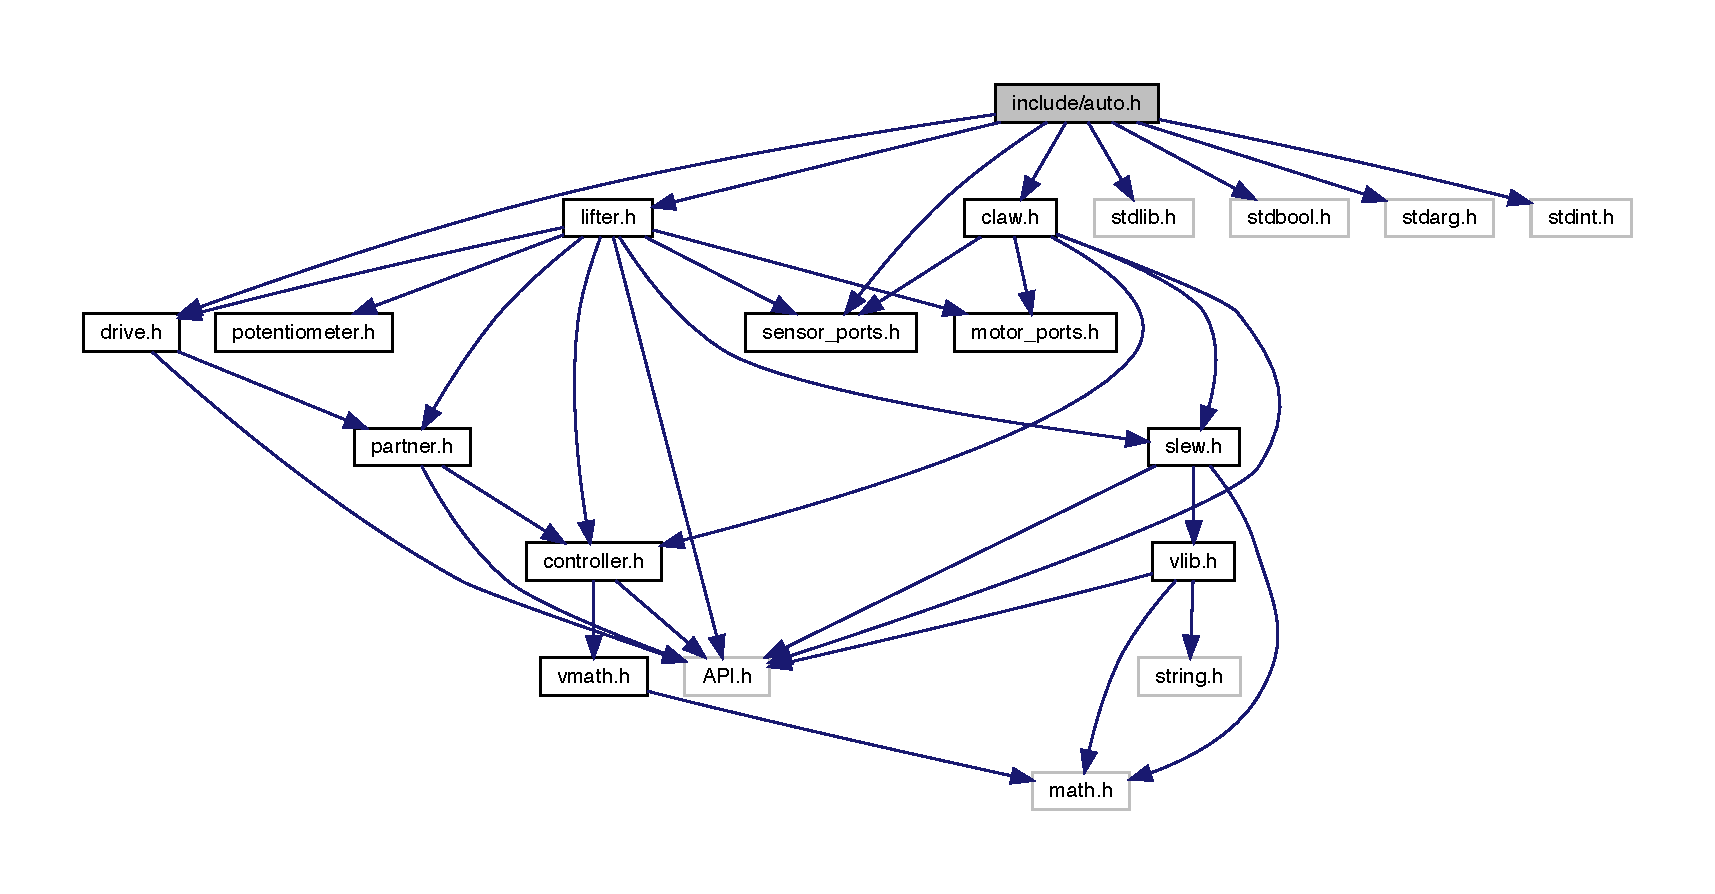
\includegraphics[width=350pt]{auto_8h__incl}
\end{center}
\end{figure}
This graph shows which files directly or indirectly include this file\+:\nopagebreak
\begin{figure}[H]
\begin{center}
\leavevmode
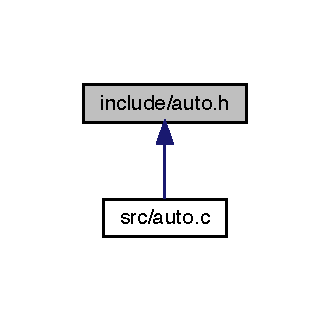
\includegraphics[width=158pt]{auto_8h__dep__incl}
\end{center}
\end{figure}
\subsection*{Macros}
\begin{DoxyCompactItemize}
\item 
\#define \textbf{ F\+R\+O\+N\+T\+\_\+\+L\+E\+F\+T\+\_\+\+I\+ME}~0
\begin{DoxyCompactList}\small\item\em Front left motor integrated motor encoder. \end{DoxyCompactList}\item 
\#define \textbf{ G\+O\+A\+L\+\_\+\+H\+E\+I\+G\+HT}~1325
\begin{DoxyCompactList}\small\item\em The height of the goal using potentiometer readings. \end{DoxyCompactList}\item 
\#define \textbf{ M\+I\+D\+\_\+\+L\+E\+F\+T\+\_\+\+D\+R\+I\+VE}~1
\begin{DoxyCompactList}\small\item\em Middle left motor integrated motor encoder. \end{DoxyCompactList}\item 
\#define \textbf{ M\+I\+D\+\_\+\+R\+I\+G\+H\+T\+\_\+\+D\+R\+I\+VE}~4
\begin{DoxyCompactList}\small\item\em Middle right motor integrated motor encoder. \end{DoxyCompactList}\item 
\#define \textbf{ S\+T\+O\+P\+\_\+\+O\+NE}~500
\begin{DoxyCompactList}\small\item\em First Stop position for stationary autonomous. \end{DoxyCompactList}\end{DoxyCompactItemize}


\subsection{Detailed Description}
Autonomous declarations and macros. 

\begin{DoxyAuthor}{Author}
Chris Jerrett 
\end{DoxyAuthor}
\begin{DoxyDate}{Date}
9/18/2017 
\end{DoxyDate}


Definition in file \textbf{ auto.\+h}.



\subsection{Macro Definition Documentation}
\mbox{\label{auto_8h_a7bc3203ebc61f8414788156a8616047c}} 
\index{auto.\+h@{auto.\+h}!F\+R\+O\+N\+T\+\_\+\+L\+E\+F\+T\+\_\+\+I\+ME@{F\+R\+O\+N\+T\+\_\+\+L\+E\+F\+T\+\_\+\+I\+ME}}
\index{F\+R\+O\+N\+T\+\_\+\+L\+E\+F\+T\+\_\+\+I\+ME@{F\+R\+O\+N\+T\+\_\+\+L\+E\+F\+T\+\_\+\+I\+ME}!auto.\+h@{auto.\+h}}
\subsubsection{F\+R\+O\+N\+T\+\_\+\+L\+E\+F\+T\+\_\+\+I\+ME}
{\footnotesize\ttfamily \#define F\+R\+O\+N\+T\+\_\+\+L\+E\+F\+T\+\_\+\+I\+ME~0}



Front left motor integrated motor encoder. 



Definition at line \textbf{ 18} of file \textbf{ auto.\+h}.

\mbox{\label{auto_8h_a83cf08759ac4ffc3ea6e3b7f9c406b3c}} 
\index{auto.\+h@{auto.\+h}!G\+O\+A\+L\+\_\+\+H\+E\+I\+G\+HT@{G\+O\+A\+L\+\_\+\+H\+E\+I\+G\+HT}}
\index{G\+O\+A\+L\+\_\+\+H\+E\+I\+G\+HT@{G\+O\+A\+L\+\_\+\+H\+E\+I\+G\+HT}!auto.\+h@{auto.\+h}}
\subsubsection{G\+O\+A\+L\+\_\+\+H\+E\+I\+G\+HT}
{\footnotesize\ttfamily \#define G\+O\+A\+L\+\_\+\+H\+E\+I\+G\+HT~1325}



The height of the goal using potentiometer readings. 



Definition at line \textbf{ 38} of file \textbf{ auto.\+h}.



Referenced by \textbf{ autonomous()}.

\mbox{\label{auto_8h_a811b1777cccc7f0e3abbec1874715f0a}} 
\index{auto.\+h@{auto.\+h}!M\+I\+D\+\_\+\+L\+E\+F\+T\+\_\+\+D\+R\+I\+VE@{M\+I\+D\+\_\+\+L\+E\+F\+T\+\_\+\+D\+R\+I\+VE}}
\index{M\+I\+D\+\_\+\+L\+E\+F\+T\+\_\+\+D\+R\+I\+VE@{M\+I\+D\+\_\+\+L\+E\+F\+T\+\_\+\+D\+R\+I\+VE}!auto.\+h@{auto.\+h}}
\subsubsection{M\+I\+D\+\_\+\+L\+E\+F\+T\+\_\+\+D\+R\+I\+VE}
{\footnotesize\ttfamily \#define M\+I\+D\+\_\+\+L\+E\+F\+T\+\_\+\+D\+R\+I\+VE~1}



Middle left motor integrated motor encoder. 



Definition at line \textbf{ 23} of file \textbf{ auto.\+h}.



Referenced by \textbf{ autonomous()}.

\mbox{\label{auto_8h_a2919b1b6b7bf06fab5b5bbf09d8d2761}} 
\index{auto.\+h@{auto.\+h}!M\+I\+D\+\_\+\+R\+I\+G\+H\+T\+\_\+\+D\+R\+I\+VE@{M\+I\+D\+\_\+\+R\+I\+G\+H\+T\+\_\+\+D\+R\+I\+VE}}
\index{M\+I\+D\+\_\+\+R\+I\+G\+H\+T\+\_\+\+D\+R\+I\+VE@{M\+I\+D\+\_\+\+R\+I\+G\+H\+T\+\_\+\+D\+R\+I\+VE}!auto.\+h@{auto.\+h}}
\subsubsection{M\+I\+D\+\_\+\+R\+I\+G\+H\+T\+\_\+\+D\+R\+I\+VE}
{\footnotesize\ttfamily \#define M\+I\+D\+\_\+\+R\+I\+G\+H\+T\+\_\+\+D\+R\+I\+VE~4}



Middle right motor integrated motor encoder. 



Definition at line \textbf{ 28} of file \textbf{ auto.\+h}.



Referenced by \textbf{ autonomous()}.

\mbox{\label{auto_8h_a67c9207ce99d4414dce28d8c42ba1d2a}} 
\index{auto.\+h@{auto.\+h}!S\+T\+O\+P\+\_\+\+O\+NE@{S\+T\+O\+P\+\_\+\+O\+NE}}
\index{S\+T\+O\+P\+\_\+\+O\+NE@{S\+T\+O\+P\+\_\+\+O\+NE}!auto.\+h@{auto.\+h}}
\subsubsection{S\+T\+O\+P\+\_\+\+O\+NE}
{\footnotesize\ttfamily \#define S\+T\+O\+P\+\_\+\+O\+NE~500}



First Stop position for stationary autonomous. 



Definition at line \textbf{ 33} of file \textbf{ auto.\+h}.


\subsection{auto.\+h}
\label{auto_8h_source}\index{include/auto.\+h@{include/auto.\+h}}

\begin{DoxyCode}
00001 
00007 \textcolor{preprocessor}{#ifndef \_AUTO\_H\_}
00008 \textcolor{preprocessor}{#define \_AUTO\_H\_}
00009 
00010 \textcolor{preprocessor}{#include "claw.h"}
00011 \textcolor{preprocessor}{#include "drive.h"}
00012 \textcolor{preprocessor}{#include "lifter.h"}
00013 \textcolor{preprocessor}{#include "sensor_ports.h"}
00014 \textcolor{preprocessor}{#include "mobile_goal_intake.h"}
00015 \textcolor{preprocessor}{#include "localization.h"}
00016 
00020 \textcolor{preprocessor}{#define FRONT\_LEFT\_IME 0}
00021 
00025 \textcolor{preprocessor}{#define MID\_LEFT\_DRIVE 1}
00026 
00030 \textcolor{preprocessor}{#define MID\_RIGHT\_DRIVE 4}
00031 
00035 \textcolor{preprocessor}{#define STOP\_ONE 500}
00036 
00040 \textcolor{preprocessor}{#define GOAL\_HEIGHT 1325}
00041 
00045 \textcolor{preprocessor}{#define DEPLOY\_HEIGHT 500}
00046 
00047 \textcolor{preprocessor}{#define LOWEST\_HEIGHT 0}
00048 
00049 \textcolor{preprocessor}{#define MOBILE\_GOAL\_HEIGHT 3090}
00050 
00051 \textcolor{preprocessor}{#define MOBILE\_GOAL\_DISTANCE 4000}
00052 
00053 \textcolor{preprocessor}{#define MAX\_HEIGHT 3090}
00054 
00055 \textcolor{preprocessor}{#define ZONE\_DISTANCE 1000}
00056 
00057 \textcolor{preprocessor}{#define HALF\_ROTATE M\_PI}
00058 
00059 \textcolor{preprocessor}{#endif}
\end{DoxyCode}

\subsection{include/battery.h File Reference}
\label{battery_8h}\index{include/battery.\+h@{include/battery.\+h}}


Battery management related functions.  


\subsubsection*{Functions}
\begin{DoxyCompactItemize}
\item 
double \textbf{ backup\+\_\+battery\+\_\+voltage} ()
\begin{DoxyCompactList}\small\item\em gets the backup battery voltage \end{DoxyCompactList}\item 
bool \textbf{ battery\+\_\+level\+\_\+acceptable} ()
\begin{DoxyCompactList}\small\item\em returns if the batteries are acceptable \end{DoxyCompactList}\item 
double \textbf{ main\+\_\+battery\+\_\+voltage} ()
\begin{DoxyCompactList}\small\item\em gets the main battery voltage \end{DoxyCompactList}\end{DoxyCompactItemize}


\subsubsection{Detailed Description}
Battery management related functions. 

\begin{DoxyAuthor}{Author}
Chris Jerrett 
\end{DoxyAuthor}
\begin{DoxyDate}{Date}
9/18/2017 
\end{DoxyDate}


Definition in file \textbf{ battery.\+h}.



\subsubsection{Function Documentation}
\mbox{\label{battery_8h_a9b1c5cf7ddddebf63796050a1d4a9969}} 
\index{battery.\+h@{battery.\+h}!backup\+\_\+battery\+\_\+voltage@{backup\+\_\+battery\+\_\+voltage}}
\index{backup\+\_\+battery\+\_\+voltage@{backup\+\_\+battery\+\_\+voltage}!battery.\+h@{battery.\+h}}
\paragraph{backup\+\_\+battery\+\_\+voltage()}
{\footnotesize\ttfamily double backup\+\_\+battery\+\_\+voltage (\begin{DoxyParamCaption}{ }\end{DoxyParamCaption})}



gets the backup battery voltage 

\begin{DoxyAuthor}{Author}
Chris Jerrett 
\end{DoxyAuthor}


Definition at line \textbf{ 14} of file \textbf{ battery.\+c}.



References \textbf{ power\+Level\+Backup()}.



Referenced by \textbf{ battery\+\_\+level\+\_\+acceptable()}.


\begin{DoxyCode}
00014 \{ \textcolor{keywordflow}{return} powerLevelBackup() / 1000.0; \}
\end{DoxyCode}
Here is the call graph for this function\+:
\nopagebreak
\begin{figure}[H]
\begin{center}
\leavevmode
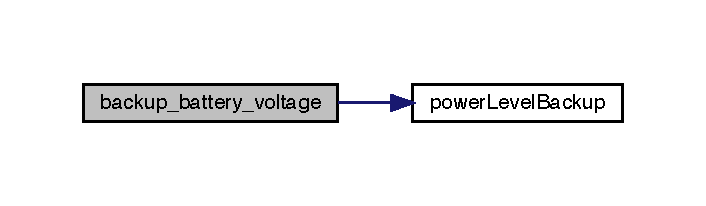
\includegraphics[width=339pt]{battery_8h_a9b1c5cf7ddddebf63796050a1d4a9969_cgraph}
\end{center}
\end{figure}
Here is the caller graph for this function\+:
\nopagebreak
\begin{figure}[H]
\begin{center}
\leavevmode
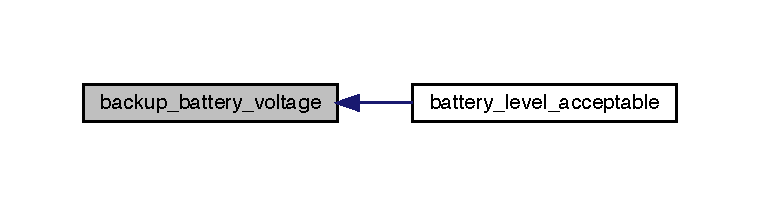
\includegraphics[width=350pt]{battery_8h_a9b1c5cf7ddddebf63796050a1d4a9969_icgraph}
\end{center}
\end{figure}
\mbox{\label{battery_8h_a1097bbb878f6e2690f8eea6cd231959a}} 
\index{battery.\+h@{battery.\+h}!battery\+\_\+level\+\_\+acceptable@{battery\+\_\+level\+\_\+acceptable}}
\index{battery\+\_\+level\+\_\+acceptable@{battery\+\_\+level\+\_\+acceptable}!battery.\+h@{battery.\+h}}
\paragraph{battery\+\_\+level\+\_\+acceptable()}
{\footnotesize\ttfamily bool battery\+\_\+level\+\_\+acceptable (\begin{DoxyParamCaption}{ }\end{DoxyParamCaption})}



returns if the batteries are acceptable 

\begin{DoxySeeAlso}{See also}
M\+I\+N\+\_\+\+M\+A\+I\+N\+\_\+\+V\+O\+L\+T\+A\+GE 

M\+I\+N\+\_\+\+B\+A\+C\+K\+U\+P\+\_\+\+V\+O\+L\+T\+A\+GE
\end{DoxySeeAlso}
\begin{DoxyAuthor}{Author}
Chris Jerrett 
\end{DoxyAuthor}


Definition at line \textbf{ 23} of file \textbf{ battery.\+c}.



References \textbf{ backup\+\_\+battery\+\_\+voltage()}, and \textbf{ main\+\_\+battery\+\_\+voltage()}.



Referenced by \textbf{ initialize()}.


\begin{DoxyCode}
00023                                 \{
00024   \textcolor{keywordflow}{if} (main_battery_voltage() < MIN\_MAIN\_VOLTAGE)
00025     \textcolor{keywordflow}{return} \textcolor{keyword}{false};
00026   \textcolor{keywordflow}{if} (backup_battery_voltage() < MIN\_BACKUP\_VOLTAGE)
00027     \textcolor{keywordflow}{return} \textcolor{keyword}{false};
00028   \textcolor{keywordflow}{return} \textcolor{keyword}{true};
00029 \}
\end{DoxyCode}
Here is the call graph for this function\+:
\nopagebreak
\begin{figure}[H]
\begin{center}
\leavevmode
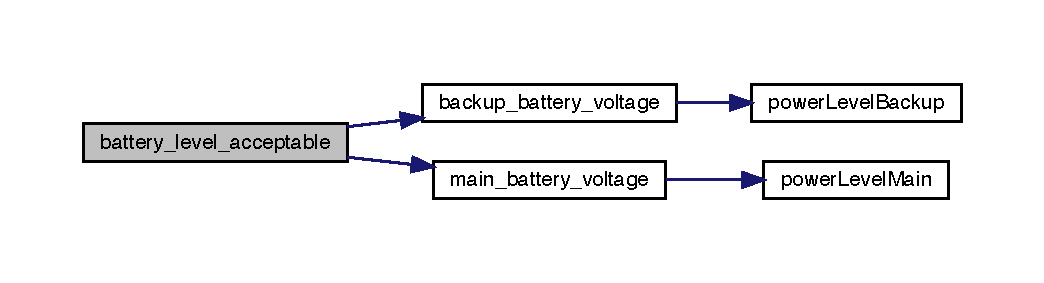
\includegraphics[width=350pt]{battery_8h_a1097bbb878f6e2690f8eea6cd231959a_cgraph}
\end{center}
\end{figure}
Here is the caller graph for this function\+:
\nopagebreak
\begin{figure}[H]
\begin{center}
\leavevmode
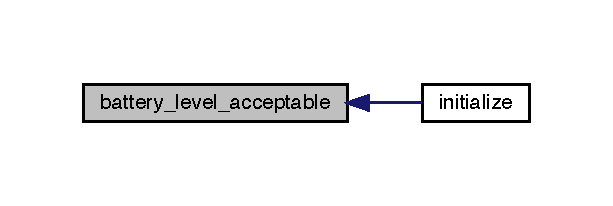
\includegraphics[width=294pt]{battery_8h_a1097bbb878f6e2690f8eea6cd231959a_icgraph}
\end{center}
\end{figure}
\mbox{\label{battery_8h_a8c92c389534fdb079698cdebeb7f2efa}} 
\index{battery.\+h@{battery.\+h}!main\+\_\+battery\+\_\+voltage@{main\+\_\+battery\+\_\+voltage}}
\index{main\+\_\+battery\+\_\+voltage@{main\+\_\+battery\+\_\+voltage}!battery.\+h@{battery.\+h}}
\paragraph{main\+\_\+battery\+\_\+voltage()}
{\footnotesize\ttfamily double main\+\_\+battery\+\_\+voltage (\begin{DoxyParamCaption}{ }\end{DoxyParamCaption})}



gets the main battery voltage 

\begin{DoxyAuthor}{Author}
Chris Jerrett 
\end{DoxyAuthor}


Definition at line \textbf{ 8} of file \textbf{ battery.\+c}.



References \textbf{ power\+Level\+Main()}.



Referenced by \textbf{ battery\+\_\+level\+\_\+acceptable()}.


\begin{DoxyCode}
00008 \{ \textcolor{keywordflow}{return} powerLevelMain() / 1000.0; \}
\end{DoxyCode}
Here is the call graph for this function\+:
\nopagebreak
\begin{figure}[H]
\begin{center}
\leavevmode
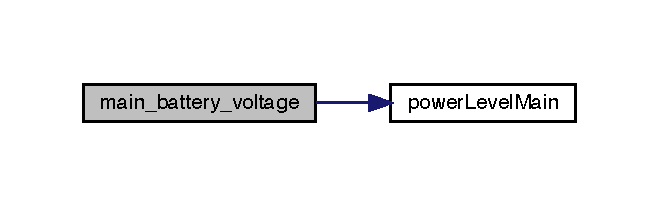
\includegraphics[width=316pt]{battery_8h_a8c92c389534fdb079698cdebeb7f2efa_cgraph}
\end{center}
\end{figure}
Here is the caller graph for this function\+:
\nopagebreak
\begin{figure}[H]
\begin{center}
\leavevmode
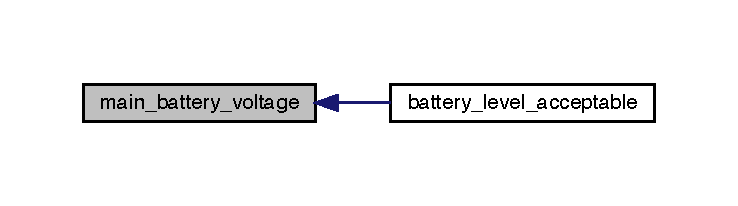
\includegraphics[width=350pt]{battery_8h_a8c92c389534fdb079698cdebeb7f2efa_icgraph}
\end{center}
\end{figure}

\section{battery.\+h}
\label{battery_8h_source}\index{include/battery.\+h@{include/battery.\+h}}

\begin{DoxyCode}
00001 
00007 \textcolor{preprocessor}{#ifndef \_BATTERY\_H\_}
00008 \textcolor{preprocessor}{#define \_BATTERY\_H\_}
00009 
00010 \textcolor{preprocessor}{#include <API.h>}
00011 
00015 \textcolor{preprocessor}{#define MIN\_MAIN\_VOLTAGE 7.8}
00016 
00020 \textcolor{preprocessor}{#define MIN\_BACKUP\_VOLTAGE 7.8}
00021 
00026 \textcolor{keywordtype}{double} main_battery_voltage();
00027 
00032 \textcolor{keywordtype}{double} backup_battery_voltage();
00033 
00041 \textcolor{keywordtype}{bool} battery_level_acceptable();
00042 
00043 \textcolor{preprocessor}{#endif}
\end{DoxyCode}

\hypertarget{claw_8h}{}\section{include/claw.h File Reference}
\label{claw_8h}\index{include/claw.\+h@{include/claw.\+h}}
{\ttfamily \#include \char`\"{}slew.\+h\char`\"{}}\newline
{\ttfamily \#include $<$A\+P\+I.\+h$>$}\newline
{\ttfamily \#include \char`\"{}controller.\+h\char`\"{}}\newline
{\ttfamily \#include \char`\"{}motor\+\_\+ports.\+h\char`\"{}}\newline
{\ttfamily \#include \char`\"{}sensor\+\_\+ports.\+h\char`\"{}}\newline
Include dependency graph for claw.\+h\+:\nopagebreak
\begin{figure}[H]
\begin{center}
\leavevmode
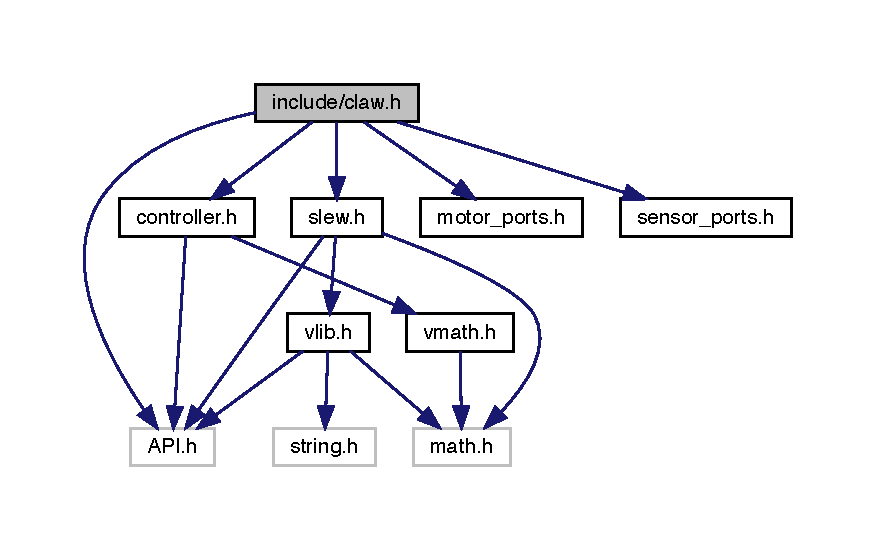
\includegraphics[width=350pt]{claw_8h__incl}
\end{center}
\end{figure}
This graph shows which files directly or indirectly include this file\+:\nopagebreak
\begin{figure}[H]
\begin{center}
\leavevmode
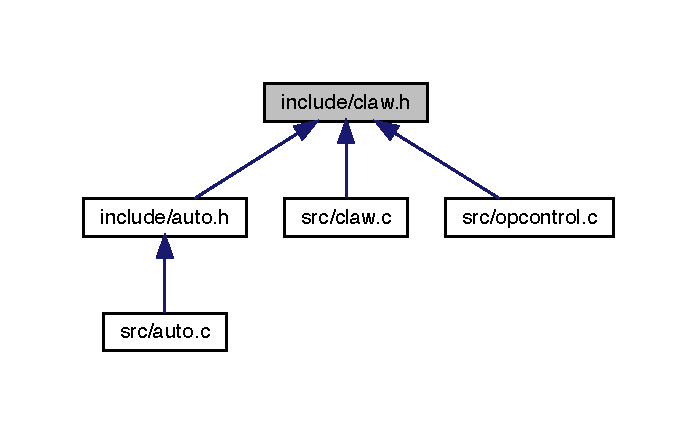
\includegraphics[width=335pt]{claw_8h__dep__incl}
\end{center}
\end{figure}
\subsection*{Macros}
\begin{DoxyCompactItemize}
\item 
\#define \hyperlink{claw_8h_af2a18397e9efae0be9470a76797b2077}{C\+L\+A\+W\+\_\+\+C\+L\+O\+SE}~\hyperlink{controller_8h_a3fa2d3bf1901157f734a584d47b25d8b}{M\+A\+S\+T\+ER}, 6, \hyperlink{_a_p_i_8h_a85e47af11e6a32e3a819f247d9f619d6}{J\+O\+Y\+\_\+\+UP}
\begin{DoxyCompactList}\small\item\em The joystick parameters for closing the claw. \end{DoxyCompactList}\item 
\#define \hyperlink{claw_8h_a78d3e6f3d4b60e1be137fdc6dd144224}{C\+L\+A\+W\+\_\+\+C\+L\+O\+S\+E\+\_\+\+V\+AL}~3000
\begin{DoxyCompactList}\small\item\em The potentiometer value for a closed claw. \end{DoxyCompactList}\item 
\#define \hyperlink{claw_8h_afa5b4892ddbbfd14068e08422386bc3f}{C\+L\+A\+W\+\_\+D}~.\+1
\begin{DoxyCompactList}\small\item\em The derivative constant for the claw P\+ID controller. \end{DoxyCompactList}\item 
\#define \hyperlink{claw_8h_a012d8ac544ee8a7a6413cee1b456773c}{C\+L\+A\+W\+\_\+I}~0
\begin{DoxyCompactList}\small\item\em The integral constant for the claw P\+ID controller. \end{DoxyCompactList}\item 
\#define \hyperlink{claw_8h_ae42993ee3f6f4a0e47f99060fe736ba0}{C\+L\+A\+W\+\_\+\+O\+P\+EN}~\hyperlink{controller_8h_a3fa2d3bf1901157f734a584d47b25d8b}{M\+A\+S\+T\+ER}, 6, \hyperlink{_a_p_i_8h_a950e3ba6cd65c992b92f36b837c52a0a}{J\+O\+Y\+\_\+\+D\+O\+WN}
\begin{DoxyCompactList}\small\item\em The joystick parameters for opening the claw. \end{DoxyCompactList}\item 
\#define \hyperlink{claw_8h_a519372d8dfa1706d706053ab035ea0b9}{C\+L\+A\+W\+\_\+\+O\+P\+E\+N\+\_\+\+V\+AL}~1500
\begin{DoxyCompactList}\small\item\em The potentiometer value for a open claw. \end{DoxyCompactList}\item 
\#define \hyperlink{claw_8h_a1f95cce21c67a6f43850ab9660c2d68a}{C\+L\+A\+W\+\_\+P}~.\+1
\begin{DoxyCompactList}\small\item\em The proportional constant for the claw P\+ID controller. \end{DoxyCompactList}\item 
\#define \hyperlink{claw_8h_ae3be50b28977dac719f086e131ba8fd7}{M\+A\+X\+\_\+\+C\+L\+A\+W\+\_\+\+S\+P\+E\+ED}~50
\begin{DoxyCompactList}\small\item\em The max motor vlaue of the claw. \end{DoxyCompactList}\item 
\#define \hyperlink{claw_8h_a7306e61a4209c74862aa81d7b3de74e5}{M\+I\+N\+\_\+\+C\+L\+A\+W\+\_\+\+S\+P\+E\+ED}~-\/50
\begin{DoxyCompactList}\small\item\em The min motor vlaue of the claw. \end{DoxyCompactList}\end{DoxyCompactItemize}
\subsection*{Enumerations}
\begin{DoxyCompactItemize}
\item 
enum \hyperlink{claw_8h_a600668fd307d596c3812126657335324}{claw\+\_\+state} \{ \hyperlink{claw_8h_a600668fd307d596c3812126657335324ab871ce9ec2796d275c09bf01abcac2cd}{C\+L\+A\+W\+\_\+\+O\+P\+E\+N\+\_\+\+S\+T\+A\+TE}, 
\hyperlink{claw_8h_a600668fd307d596c3812126657335324a3948a2d760f710e9087edded3df98b5f}{C\+L\+A\+W\+\_\+\+C\+L\+O\+S\+E\+\_\+\+S\+T\+A\+TE}
 \}\begin{DoxyCompactList}\small\item\em The different states of the claw. \end{DoxyCompactList}
\end{DoxyCompactItemize}
\subsection*{Functions}
\begin{DoxyCompactItemize}
\item 
void \hyperlink{claw_8h_ac42dd40dbb37219295286859c6b068c2}{close\+\_\+claw} ()
\begin{DoxyCompactList}\small\item\em Drives the motors to close the claw. \end{DoxyCompactList}\item 
unsigned int \hyperlink{claw_8h_addd2004effae7c94400aed1fe6a90ead}{get\+Claw\+Ticks} ()
\begin{DoxyCompactList}\small\item\em Gets the claw position in potentiometer ticks. \end{DoxyCompactList}\item 
void \hyperlink{claw_8h_a03023ca28f671b9fa7bac07782ccd8c1}{open\+\_\+claw} ()
\begin{DoxyCompactList}\small\item\em Drives the motors to open the claw. \end{DoxyCompactList}\item 
void \hyperlink{claw_8h_a3a57f998b1884d39b0cc786689f7086f}{set\+\_\+claw\+\_\+motor} (const int v)
\begin{DoxyCompactList}\small\item\em sets the claw motor speed \end{DoxyCompactList}\item 
void \hyperlink{claw_8h_a0122b78972344264b8a276a559cfce4a}{update\+\_\+claw} ()
\begin{DoxyCompactList}\small\item\em Updates the claw motor values. \end{DoxyCompactList}\end{DoxyCompactItemize}


\subsection{Macro Definition Documentation}
\mbox{\Hypertarget{claw_8h_af2a18397e9efae0be9470a76797b2077}\label{claw_8h_af2a18397e9efae0be9470a76797b2077}} 
\index{claw.\+h@{claw.\+h}!C\+L\+A\+W\+\_\+\+C\+L\+O\+SE@{C\+L\+A\+W\+\_\+\+C\+L\+O\+SE}}
\index{C\+L\+A\+W\+\_\+\+C\+L\+O\+SE@{C\+L\+A\+W\+\_\+\+C\+L\+O\+SE}!claw.\+h@{claw.\+h}}
\subsubsection{\texorpdfstring{C\+L\+A\+W\+\_\+\+C\+L\+O\+SE}{CLAW\_CLOSE}}
{\footnotesize\ttfamily \#define C\+L\+A\+W\+\_\+\+C\+L\+O\+SE~\hyperlink{controller_8h_a3fa2d3bf1901157f734a584d47b25d8b}{M\+A\+S\+T\+ER}, 6, \hyperlink{_a_p_i_8h_a85e47af11e6a32e3a819f247d9f619d6}{J\+O\+Y\+\_\+\+UP}}



The joystick parameters for closing the claw. 

\begin{DoxyAuthor}{Author}
Chris Jerrett 
\end{DoxyAuthor}


Definition at line 41 of file claw.\+h.



Referenced by update\+\_\+claw().

\mbox{\Hypertarget{claw_8h_a78d3e6f3d4b60e1be137fdc6dd144224}\label{claw_8h_a78d3e6f3d4b60e1be137fdc6dd144224}} 
\index{claw.\+h@{claw.\+h}!C\+L\+A\+W\+\_\+\+C\+L\+O\+S\+E\+\_\+\+V\+AL@{C\+L\+A\+W\+\_\+\+C\+L\+O\+S\+E\+\_\+\+V\+AL}}
\index{C\+L\+A\+W\+\_\+\+C\+L\+O\+S\+E\+\_\+\+V\+AL@{C\+L\+A\+W\+\_\+\+C\+L\+O\+S\+E\+\_\+\+V\+AL}!claw.\+h@{claw.\+h}}
\subsubsection{\texorpdfstring{C\+L\+A\+W\+\_\+\+C\+L\+O\+S\+E\+\_\+\+V\+AL}{CLAW\_CLOSE\_VAL}}
{\footnotesize\ttfamily \#define C\+L\+A\+W\+\_\+\+C\+L\+O\+S\+E\+\_\+\+V\+AL~3000}



The potentiometer value for a closed claw. 

\begin{DoxyAuthor}{Author}
Chris Jerrett 
\end{DoxyAuthor}


Definition at line 53 of file claw.\+h.



Referenced by update\+\_\+claw().

\mbox{\Hypertarget{claw_8h_afa5b4892ddbbfd14068e08422386bc3f}\label{claw_8h_afa5b4892ddbbfd14068e08422386bc3f}} 
\index{claw.\+h@{claw.\+h}!C\+L\+A\+W\+\_\+D@{C\+L\+A\+W\+\_\+D}}
\index{C\+L\+A\+W\+\_\+D@{C\+L\+A\+W\+\_\+D}!claw.\+h@{claw.\+h}}
\subsubsection{\texorpdfstring{C\+L\+A\+W\+\_\+D}{CLAW\_D}}
{\footnotesize\ttfamily \#define C\+L\+A\+W\+\_\+D~.\+1}



The derivative constant for the claw P\+ID controller. 

\begin{DoxyAuthor}{Author}
Chris Jerrett 
\end{DoxyAuthor}


Definition at line 19 of file claw.\+h.

\mbox{\Hypertarget{claw_8h_a012d8ac544ee8a7a6413cee1b456773c}\label{claw_8h_a012d8ac544ee8a7a6413cee1b456773c}} 
\index{claw.\+h@{claw.\+h}!C\+L\+A\+W\+\_\+I@{C\+L\+A\+W\+\_\+I}}
\index{C\+L\+A\+W\+\_\+I@{C\+L\+A\+W\+\_\+I}!claw.\+h@{claw.\+h}}
\subsubsection{\texorpdfstring{C\+L\+A\+W\+\_\+I}{CLAW\_I}}
{\footnotesize\ttfamily \#define C\+L\+A\+W\+\_\+I~0}



The integral constant for the claw P\+ID controller. 

\begin{DoxyAuthor}{Author}
Chris Jerrett 
\end{DoxyAuthor}


Definition at line 24 of file claw.\+h.

\mbox{\Hypertarget{claw_8h_ae42993ee3f6f4a0e47f99060fe736ba0}\label{claw_8h_ae42993ee3f6f4a0e47f99060fe736ba0}} 
\index{claw.\+h@{claw.\+h}!C\+L\+A\+W\+\_\+\+O\+P\+EN@{C\+L\+A\+W\+\_\+\+O\+P\+EN}}
\index{C\+L\+A\+W\+\_\+\+O\+P\+EN@{C\+L\+A\+W\+\_\+\+O\+P\+EN}!claw.\+h@{claw.\+h}}
\subsubsection{\texorpdfstring{C\+L\+A\+W\+\_\+\+O\+P\+EN}{CLAW\_OPEN}}
{\footnotesize\ttfamily \#define C\+L\+A\+W\+\_\+\+O\+P\+EN~\hyperlink{controller_8h_a3fa2d3bf1901157f734a584d47b25d8b}{M\+A\+S\+T\+ER}, 6, \hyperlink{_a_p_i_8h_a950e3ba6cd65c992b92f36b837c52a0a}{J\+O\+Y\+\_\+\+D\+O\+WN}}



The joystick parameters for opening the claw. 

\begin{DoxyAuthor}{Author}
Chris Jerrett 
\end{DoxyAuthor}


Definition at line 47 of file claw.\+h.



Referenced by update\+\_\+claw().

\mbox{\Hypertarget{claw_8h_a519372d8dfa1706d706053ab035ea0b9}\label{claw_8h_a519372d8dfa1706d706053ab035ea0b9}} 
\index{claw.\+h@{claw.\+h}!C\+L\+A\+W\+\_\+\+O\+P\+E\+N\+\_\+\+V\+AL@{C\+L\+A\+W\+\_\+\+O\+P\+E\+N\+\_\+\+V\+AL}}
\index{C\+L\+A\+W\+\_\+\+O\+P\+E\+N\+\_\+\+V\+AL@{C\+L\+A\+W\+\_\+\+O\+P\+E\+N\+\_\+\+V\+AL}!claw.\+h@{claw.\+h}}
\subsubsection{\texorpdfstring{C\+L\+A\+W\+\_\+\+O\+P\+E\+N\+\_\+\+V\+AL}{CLAW\_OPEN\_VAL}}
{\footnotesize\ttfamily \#define C\+L\+A\+W\+\_\+\+O\+P\+E\+N\+\_\+\+V\+AL~1500}



The potentiometer value for a open claw. 

\begin{DoxyAuthor}{Author}
Chris Jerrett 
\end{DoxyAuthor}


Definition at line 59 of file claw.\+h.



Referenced by update\+\_\+claw().

\mbox{\Hypertarget{claw_8h_a1f95cce21c67a6f43850ab9660c2d68a}\label{claw_8h_a1f95cce21c67a6f43850ab9660c2d68a}} 
\index{claw.\+h@{claw.\+h}!C\+L\+A\+W\+\_\+P@{C\+L\+A\+W\+\_\+P}}
\index{C\+L\+A\+W\+\_\+P@{C\+L\+A\+W\+\_\+P}!claw.\+h@{claw.\+h}}
\subsubsection{\texorpdfstring{C\+L\+A\+W\+\_\+P}{CLAW\_P}}
{\footnotesize\ttfamily \#define C\+L\+A\+W\+\_\+P~.\+1}



The proportional constant for the claw P\+ID controller. 

\begin{DoxyAuthor}{Author}
Chris Jerrett 
\end{DoxyAuthor}


Definition at line 14 of file claw.\+h.



Referenced by update\+\_\+claw().

\mbox{\Hypertarget{claw_8h_ae3be50b28977dac719f086e131ba8fd7}\label{claw_8h_ae3be50b28977dac719f086e131ba8fd7}} 
\index{claw.\+h@{claw.\+h}!M\+A\+X\+\_\+\+C\+L\+A\+W\+\_\+\+S\+P\+E\+ED@{M\+A\+X\+\_\+\+C\+L\+A\+W\+\_\+\+S\+P\+E\+ED}}
\index{M\+A\+X\+\_\+\+C\+L\+A\+W\+\_\+\+S\+P\+E\+ED@{M\+A\+X\+\_\+\+C\+L\+A\+W\+\_\+\+S\+P\+E\+ED}!claw.\+h@{claw.\+h}}
\subsubsection{\texorpdfstring{M\+A\+X\+\_\+\+C\+L\+A\+W\+\_\+\+S\+P\+E\+ED}{MAX\_CLAW\_SPEED}}
{\footnotesize\ttfamily \#define M\+A\+X\+\_\+\+C\+L\+A\+W\+\_\+\+S\+P\+E\+ED~50}



The max motor vlaue of the claw. 

\begin{DoxyAuthor}{Author}
Chris Jerrett 
\end{DoxyAuthor}


Definition at line 30 of file claw.\+h.



Referenced by open\+\_\+claw().

\mbox{\Hypertarget{claw_8h_a7306e61a4209c74862aa81d7b3de74e5}\label{claw_8h_a7306e61a4209c74862aa81d7b3de74e5}} 
\index{claw.\+h@{claw.\+h}!M\+I\+N\+\_\+\+C\+L\+A\+W\+\_\+\+S\+P\+E\+ED@{M\+I\+N\+\_\+\+C\+L\+A\+W\+\_\+\+S\+P\+E\+ED}}
\index{M\+I\+N\+\_\+\+C\+L\+A\+W\+\_\+\+S\+P\+E\+ED@{M\+I\+N\+\_\+\+C\+L\+A\+W\+\_\+\+S\+P\+E\+ED}!claw.\+h@{claw.\+h}}
\subsubsection{\texorpdfstring{M\+I\+N\+\_\+\+C\+L\+A\+W\+\_\+\+S\+P\+E\+ED}{MIN\_CLAW\_SPEED}}
{\footnotesize\ttfamily \#define M\+I\+N\+\_\+\+C\+L\+A\+W\+\_\+\+S\+P\+E\+ED~-\/50}



The min motor vlaue of the claw. 

\begin{DoxyAuthor}{Author}
Chris Jerrett 
\end{DoxyAuthor}


Definition at line 35 of file claw.\+h.



Referenced by close\+\_\+claw().



\subsection{Enumeration Type Documentation}
\mbox{\Hypertarget{claw_8h_a600668fd307d596c3812126657335324}\label{claw_8h_a600668fd307d596c3812126657335324}} 
\index{claw.\+h@{claw.\+h}!claw\+\_\+state@{claw\+\_\+state}}
\index{claw\+\_\+state@{claw\+\_\+state}!claw.\+h@{claw.\+h}}
\subsubsection{\texorpdfstring{claw\+\_\+state}{claw\_state}}
{\footnotesize\ttfamily enum \hyperlink{claw_8h_a600668fd307d596c3812126657335324}{claw\+\_\+state}}



The different states of the claw. 

\begin{DoxyAuthor}{Author}
Chris Jerrett 
\end{DoxyAuthor}
\begin{DoxyEnumFields}{Enumerator}
\raisebox{\heightof{T}}[0pt][0pt]{\index{C\+L\+A\+W\+\_\+\+O\+P\+E\+N\+\_\+\+S\+T\+A\+TE@{C\+L\+A\+W\+\_\+\+O\+P\+E\+N\+\_\+\+S\+T\+A\+TE}!claw.\+h@{claw.\+h}}\index{claw.\+h@{claw.\+h}!C\+L\+A\+W\+\_\+\+O\+P\+E\+N\+\_\+\+S\+T\+A\+TE@{C\+L\+A\+W\+\_\+\+O\+P\+E\+N\+\_\+\+S\+T\+A\+TE}}}\mbox{\Hypertarget{claw_8h_a600668fd307d596c3812126657335324ab871ce9ec2796d275c09bf01abcac2cd}\label{claw_8h_a600668fd307d596c3812126657335324ab871ce9ec2796d275c09bf01abcac2cd}} 
C\+L\+A\+W\+\_\+\+O\+P\+E\+N\+\_\+\+S\+T\+A\+TE&\\
\hline

\raisebox{\heightof{T}}[0pt][0pt]{\index{C\+L\+A\+W\+\_\+\+C\+L\+O\+S\+E\+\_\+\+S\+T\+A\+TE@{C\+L\+A\+W\+\_\+\+C\+L\+O\+S\+E\+\_\+\+S\+T\+A\+TE}!claw.\+h@{claw.\+h}}\index{claw.\+h@{claw.\+h}!C\+L\+A\+W\+\_\+\+C\+L\+O\+S\+E\+\_\+\+S\+T\+A\+TE@{C\+L\+A\+W\+\_\+\+C\+L\+O\+S\+E\+\_\+\+S\+T\+A\+TE}}}\mbox{\Hypertarget{claw_8h_a600668fd307d596c3812126657335324a3948a2d760f710e9087edded3df98b5f}\label{claw_8h_a600668fd307d596c3812126657335324a3948a2d760f710e9087edded3df98b5f}} 
C\+L\+A\+W\+\_\+\+C\+L\+O\+S\+E\+\_\+\+S\+T\+A\+TE&\\
\hline

\end{DoxyEnumFields}


Definition at line 95 of file claw.\+h.


\begin{DoxyCode}
95                 \{
96   \hyperlink{claw_8h_a600668fd307d596c3812126657335324ab871ce9ec2796d275c09bf01abcac2cd}{CLAW\_OPEN\_STATE},
97   \hyperlink{claw_8h_a600668fd307d596c3812126657335324a3948a2d760f710e9087edded3df98b5f}{CLAW\_CLOSE\_STATE}
98 \};
\end{DoxyCode}


\subsection{Function Documentation}
\mbox{\Hypertarget{claw_8h_ac42dd40dbb37219295286859c6b068c2}\label{claw_8h_ac42dd40dbb37219295286859c6b068c2}} 
\index{claw.\+h@{claw.\+h}!close\+\_\+claw@{close\+\_\+claw}}
\index{close\+\_\+claw@{close\+\_\+claw}!claw.\+h@{claw.\+h}}
\subsubsection{\texorpdfstring{close\+\_\+claw()}{close\_claw()}}
{\footnotesize\ttfamily void close\+\_\+claw (\begin{DoxyParamCaption}{ }\end{DoxyParamCaption})}



Drives the motors to close the claw. 

\begin{DoxyAuthor}{Author}
Chris Jerrett 
\end{DoxyAuthor}


Definition at line 37 of file claw.\+c.



References C\+L\+A\+W\+\_\+\+M\+O\+T\+OR, M\+I\+N\+\_\+\+C\+L\+A\+W\+\_\+\+S\+P\+E\+ED, and set\+\_\+motor\+\_\+immediate().



Referenced by autonomous().


\begin{DoxyCode}
37                   \{
38   \hyperlink{slew_8h_a9f8b8ae577ef938622024545711f0151}{set\_motor\_immediate}(\hyperlink{motor__ports_8h_aa3bcf05406f673f735df023643f347bb}{CLAW\_MOTOR}, \hyperlink{claw_8h_a7306e61a4209c74862aa81d7b3de74e5}{MIN\_CLAW\_SPEED});
39 \}
\end{DoxyCode}
Here is the call graph for this function\+:\nopagebreak
\begin{figure}[H]
\begin{center}
\leavevmode
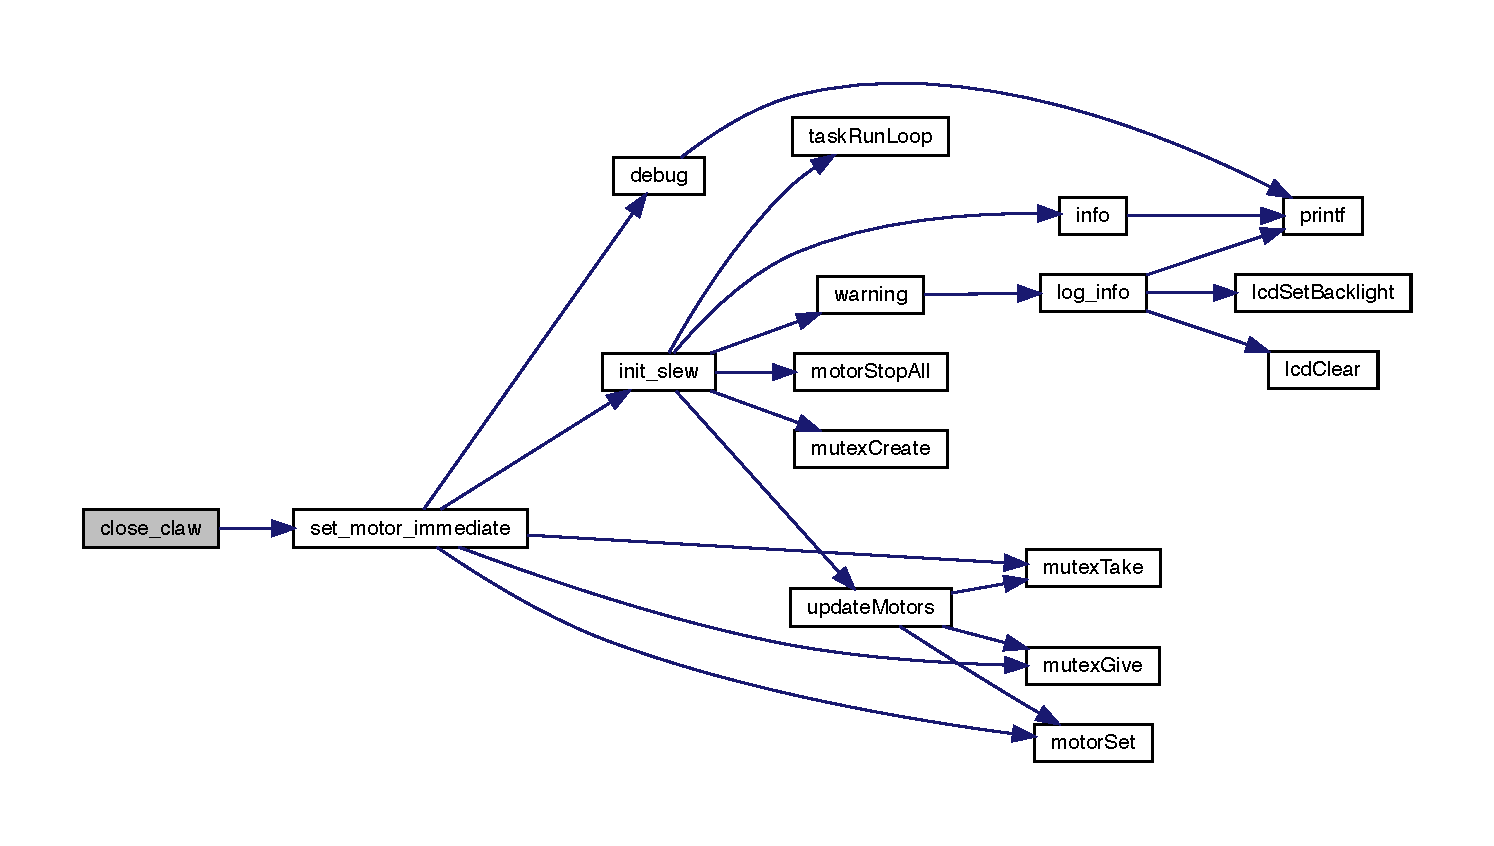
\includegraphics[width=350pt]{claw_8h_ac42dd40dbb37219295286859c6b068c2_cgraph}
\end{center}
\end{figure}
Here is the caller graph for this function\+:\nopagebreak
\begin{figure}[H]
\begin{center}
\leavevmode
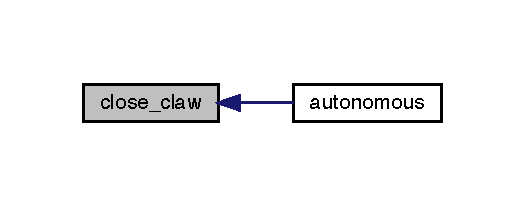
\includegraphics[width=252pt]{claw_8h_ac42dd40dbb37219295286859c6b068c2_icgraph}
\end{center}
\end{figure}
\mbox{\Hypertarget{claw_8h_addd2004effae7c94400aed1fe6a90ead}\label{claw_8h_addd2004effae7c94400aed1fe6a90ead}} 
\index{claw.\+h@{claw.\+h}!get\+Claw\+Ticks@{get\+Claw\+Ticks}}
\index{get\+Claw\+Ticks@{get\+Claw\+Ticks}!claw.\+h@{claw.\+h}}
\subsubsection{\texorpdfstring{get\+Claw\+Ticks()}{getClawTicks()}}
{\footnotesize\ttfamily unsigned int get\+Claw\+Ticks (\begin{DoxyParamCaption}{ }\end{DoxyParamCaption})}



Gets the claw position in potentiometer ticks. 

\begin{DoxyAuthor}{Author}
Chris Jerrett 
\end{DoxyAuthor}


Definition at line 29 of file claw.\+c.



References analog\+Read(), and C\+L\+A\+W\+\_\+\+P\+OT.



Referenced by update\+\_\+claw().


\begin{DoxyCode}
29                            \{
30   \textcolor{keywordflow}{return} \hyperlink{_a_p_i_8h_a5da86064604c539c2b6a5e2993289108}{analogRead}(\hyperlink{sensor__ports_8h_a780fc8672d5a3ae3cfa4ac20278ffc46}{CLAW\_POT});
31 \}
\end{DoxyCode}
Here is the call graph for this function\+:\nopagebreak
\begin{figure}[H]
\begin{center}
\leavevmode
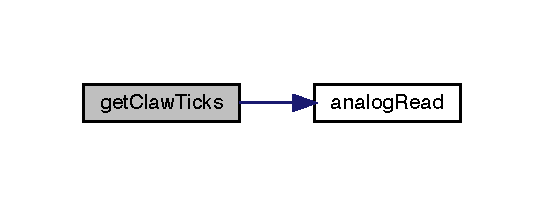
\includegraphics[width=261pt]{claw_8h_addd2004effae7c94400aed1fe6a90ead_cgraph}
\end{center}
\end{figure}
Here is the caller graph for this function\+:\nopagebreak
\begin{figure}[H]
\begin{center}
\leavevmode
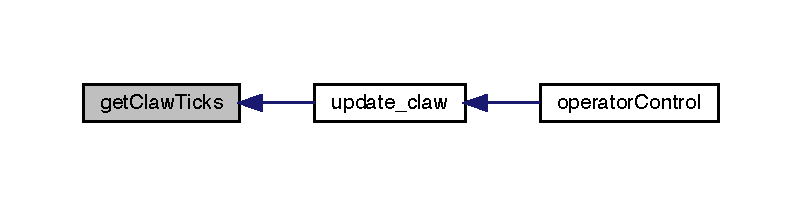
\includegraphics[width=350pt]{claw_8h_addd2004effae7c94400aed1fe6a90ead_icgraph}
\end{center}
\end{figure}
\mbox{\Hypertarget{claw_8h_a03023ca28f671b9fa7bac07782ccd8c1}\label{claw_8h_a03023ca28f671b9fa7bac07782ccd8c1}} 
\index{claw.\+h@{claw.\+h}!open\+\_\+claw@{open\+\_\+claw}}
\index{open\+\_\+claw@{open\+\_\+claw}!claw.\+h@{claw.\+h}}
\subsubsection{\texorpdfstring{open\+\_\+claw()}{open\_claw()}}
{\footnotesize\ttfamily void open\+\_\+claw (\begin{DoxyParamCaption}{ }\end{DoxyParamCaption})}



Drives the motors to open the claw. 

\begin{DoxyAuthor}{Author}
Chris Jerrett 
\end{DoxyAuthor}


Definition at line 33 of file claw.\+c.



References C\+L\+A\+W\+\_\+\+M\+O\+T\+OR, M\+A\+X\+\_\+\+C\+L\+A\+W\+\_\+\+S\+P\+E\+ED, and set\+\_\+motor\+\_\+immediate().



Referenced by autonomous().


\begin{DoxyCode}
33                  \{
34   \hyperlink{slew_8h_a9f8b8ae577ef938622024545711f0151}{set\_motor\_immediate}(\hyperlink{motor__ports_8h_aa3bcf05406f673f735df023643f347bb}{CLAW\_MOTOR}, \hyperlink{claw_8h_ae3be50b28977dac719f086e131ba8fd7}{MAX\_CLAW\_SPEED});
35 \}
\end{DoxyCode}
Here is the call graph for this function\+:\nopagebreak
\begin{figure}[H]
\begin{center}
\leavevmode
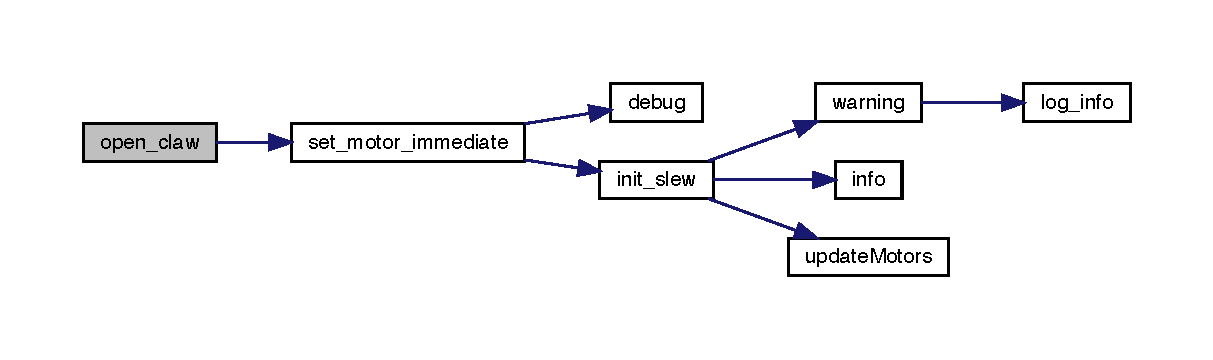
\includegraphics[width=350pt]{claw_8h_a03023ca28f671b9fa7bac07782ccd8c1_cgraph}
\end{center}
\end{figure}
Here is the caller graph for this function\+:\nopagebreak
\begin{figure}[H]
\begin{center}
\leavevmode
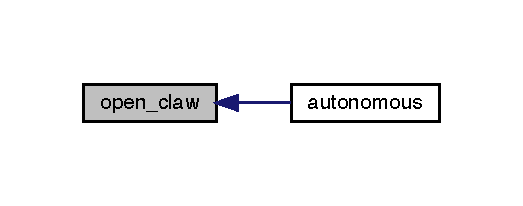
\includegraphics[width=251pt]{claw_8h_a03023ca28f671b9fa7bac07782ccd8c1_icgraph}
\end{center}
\end{figure}
\mbox{\Hypertarget{claw_8h_a3a57f998b1884d39b0cc786689f7086f}\label{claw_8h_a3a57f998b1884d39b0cc786689f7086f}} 
\index{claw.\+h@{claw.\+h}!set\+\_\+claw\+\_\+motor@{set\+\_\+claw\+\_\+motor}}
\index{set\+\_\+claw\+\_\+motor@{set\+\_\+claw\+\_\+motor}!claw.\+h@{claw.\+h}}
\subsubsection{\texorpdfstring{set\+\_\+claw\+\_\+motor()}{set\_claw\_motor()}}
{\footnotesize\ttfamily void set\+\_\+claw\+\_\+motor (\begin{DoxyParamCaption}\item[{const int}]{v }\end{DoxyParamCaption})}



sets the claw motor speed 

\begin{DoxyAuthor}{Author}
Chris Jerrett 
\end{DoxyAuthor}


Definition at line 25 of file claw.\+c.



References C\+L\+A\+W\+\_\+\+M\+O\+T\+OR, and set\+\_\+motor\+\_\+immediate().



Referenced by update\+\_\+claw().


\begin{DoxyCode}
25                                 \{
26   \hyperlink{slew_8h_a9f8b8ae577ef938622024545711f0151}{set\_motor\_immediate}(\hyperlink{motor__ports_8h_aa3bcf05406f673f735df023643f347bb}{CLAW\_MOTOR}, v);
27 \}
\end{DoxyCode}
Here is the call graph for this function\+:\nopagebreak
\begin{figure}[H]
\begin{center}
\leavevmode
\includegraphics[width=350pt]{claw_8h_a3a57f998b1884d39b0cc786689f7086f_cgraph}
\end{center}
\end{figure}
Here is the caller graph for this function\+:\nopagebreak
\begin{figure}[H]
\begin{center}
\leavevmode
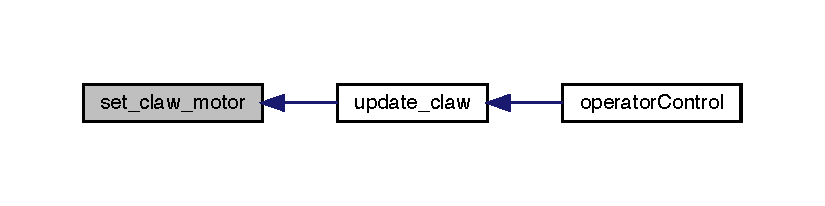
\includegraphics[width=350pt]{claw_8h_a3a57f998b1884d39b0cc786689f7086f_icgraph}
\end{center}
\end{figure}
\mbox{\Hypertarget{claw_8h_a0122b78972344264b8a276a559cfce4a}\label{claw_8h_a0122b78972344264b8a276a559cfce4a}} 
\index{claw.\+h@{claw.\+h}!update\+\_\+claw@{update\+\_\+claw}}
\index{update\+\_\+claw@{update\+\_\+claw}!claw.\+h@{claw.\+h}}
\subsubsection{\texorpdfstring{update\+\_\+claw()}{update\_claw()}}
{\footnotesize\ttfamily void update\+\_\+claw (\begin{DoxyParamCaption}{ }\end{DoxyParamCaption})}



Updates the claw motor values. 

\begin{DoxyAuthor}{Author}
Chris Jerrett 
\end{DoxyAuthor}


Definition at line 3 of file claw.\+c.



References C\+L\+A\+W\+\_\+\+C\+L\+O\+SE, C\+L\+A\+W\+\_\+\+C\+L\+O\+S\+E\+\_\+\+S\+T\+A\+TE, C\+L\+A\+W\+\_\+\+C\+L\+O\+S\+E\+\_\+\+V\+AL, C\+L\+A\+W\+\_\+\+O\+P\+EN, C\+L\+A\+W\+\_\+\+O\+P\+E\+N\+\_\+\+S\+T\+A\+TE, C\+L\+A\+W\+\_\+\+O\+P\+E\+N\+\_\+\+V\+AL, C\+L\+A\+W\+\_\+P, get\+Claw\+Ticks(), joystick\+Get\+Digital(), and set\+\_\+claw\+\_\+motor().



Referenced by operator\+Control().


\begin{DoxyCode}
3                    \{
4   \textcolor{keyword}{static} \textcolor{keywordtype}{int} last\_error = 0;
5   \textcolor{keyword}{static} \textcolor{keyword}{enum} \hyperlink{claw_8h_a600668fd307d596c3812126657335324}{claw\_state} state = \hyperlink{claw_8h_a600668fd307d596c3812126657335324ab871ce9ec2796d275c09bf01abcac2cd}{CLAW\_OPEN\_STATE};
6   \textcolor{keywordflow}{if}(\hyperlink{_a_p_i_8h_a792f1a80c62a63e764cf64aabf95db92}{joystickGetDigital}(\hyperlink{claw_8h_af2a18397e9efae0be9470a76797b2077}{CLAW\_CLOSE}))\{
7     state = \hyperlink{claw_8h_a600668fd307d596c3812126657335324a3948a2d760f710e9087edded3df98b5f}{CLAW\_CLOSE\_STATE};
8   \}
9   \textcolor{keywordflow}{else} \textcolor{keywordflow}{if}(\hyperlink{_a_p_i_8h_a792f1a80c62a63e764cf64aabf95db92}{joystickGetDigital}(\hyperlink{claw_8h_ae42993ee3f6f4a0e47f99060fe736ba0}{CLAW\_OPEN}))\{
10     state = \hyperlink{claw_8h_a600668fd307d596c3812126657335324ab871ce9ec2796d275c09bf01abcac2cd}{CLAW\_OPEN\_STATE};
11   \} \textcolor{keywordflow}{else} \{
12     \textcolor{keywordtype}{int} p = 0;
13     \textcolor{keywordflow}{if}(state == \hyperlink{claw_8h_a600668fd307d596c3812126657335324ab871ce9ec2796d275c09bf01abcac2cd}{CLAW\_OPEN\_STATE}) \{
14       p = \hyperlink{claw_8c_addd2004effae7c94400aed1fe6a90ead}{getClawTicks}() - \hyperlink{claw_8h_a519372d8dfa1706d706053ab035ea0b9}{CLAW\_OPEN\_VAL};
15     \} \textcolor{keywordflow}{else} \{
16       p = \hyperlink{claw_8c_addd2004effae7c94400aed1fe6a90ead}{getClawTicks}() - \hyperlink{claw_8h_a78d3e6f3d4b60e1be137fdc6dd144224}{CLAW\_CLOSE\_VAL};
17     \}
18 
19     \textcolor{keywordtype}{int} d = (p - last\_error);
20     \textcolor{keywordtype}{int} motor = \hyperlink{claw_8h_a1f95cce21c67a6f43850ab9660c2d68a}{CLAW\_P} * p;
21     \hyperlink{claw_8c_a3a57f998b1884d39b0cc786689f7086f}{set\_claw\_motor}(motor);
22   \}
23 \}
\end{DoxyCode}
Here is the call graph for this function\+:\nopagebreak
\begin{figure}[H]
\begin{center}
\leavevmode
\includegraphics[width=350pt]{claw_8h_a0122b78972344264b8a276a559cfce4a_cgraph}
\end{center}
\end{figure}
Here is the caller graph for this function\+:\nopagebreak
\begin{figure}[H]
\begin{center}
\leavevmode
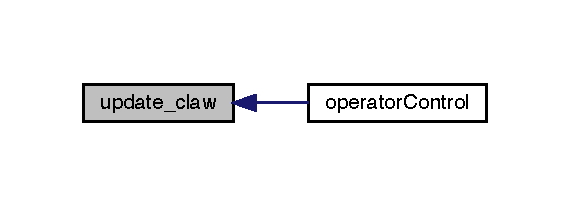
\includegraphics[width=274pt]{claw_8h_a0122b78972344264b8a276a559cfce4a_icgraph}
\end{center}
\end{figure}

\subsection{claw.\+h}
\label{claw_8h_source}\index{include/claw.\+h@{include/claw.\+h}}

\begin{DoxyCode}
00001 
00007 \textcolor{preprocessor}{#ifndef \_CLAW\_H\_}
00008 \textcolor{preprocessor}{#define \_CLAW\_H\_}
00009 
00010 \textcolor{preprocessor}{#include "controller.h"}
00011 \textcolor{preprocessor}{#include "motor_ports.h"}
00012 \textcolor{preprocessor}{#include "sensor_ports.h"}
00013 \textcolor{preprocessor}{#include "slew.h"}
00014 \textcolor{preprocessor}{#include <API.h>}
00015 
00020 \textcolor{preprocessor}{#define MAX\_CLAW\_SPEED 127}
00021 
00025 \textcolor{preprocessor}{#define MIN\_CLAW\_SPEED -127}
00026 
00031 \textcolor{preprocessor}{#define CLAW\_CLOSE MASTER, 5, JOY\_UP}
00032 
00037 \textcolor{preprocessor}{#define CLAW\_OPEN MASTER, 5, JOY\_DOWN}
00038 
00043 \textcolor{preprocessor}{#define CLAW\_CLOSE\_VAL 3000}
00044 
00049 \textcolor{preprocessor}{#define CLAW\_OPEN\_VAL 1500}
00050 
00055 \textcolor{keywordtype}{void} update_claw();
00056 
00061 \textcolor{keywordtype}{void} set_claw_motor(\textcolor{keyword}{const} \textcolor{keywordtype}{int} v);
00062 
00067 \textcolor{keywordtype}{unsigned} \textcolor{keywordtype}{int} getClawTicks();
00068 
00073 \textcolor{keywordtype}{void} open_claw();
00074 
00079 \textcolor{keywordtype}{void} close_claw();
00080 
00085 \textcolor{keyword}{enum} claw_state \{ CLAW_OPEN_STATE, CLAW_CLOSE_STATE, CLAW_NEUTRAL_STATE \};
00086 
00087 \textcolor{preprocessor}{#endif}
\end{DoxyCode}

\section{include/controller.h File Reference}
\label{controller_8h}\index{include/controller.\+h@{include/controller.\+h}}


controller definitions, macros and functions to assist with usig the vex controllers.  


{\ttfamily \#include \char`\"{}vmath.\+h\char`\"{}}\newline
{\ttfamily \#include $<$A\+P\+I.\+h$>$}\newline
Include dependency graph for controller.\+h\+:\nopagebreak
\begin{figure}[H]
\begin{center}
\leavevmode
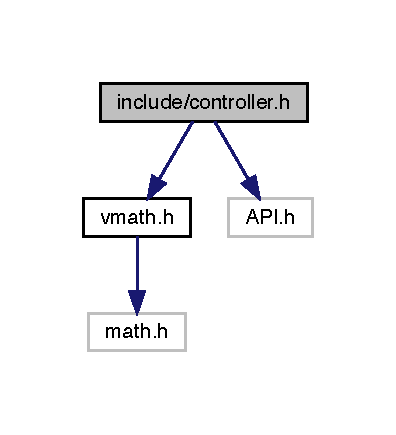
\includegraphics[width=190pt]{controller_8h__incl}
\end{center}
\end{figure}
This graph shows which files directly or indirectly include this file\+:\nopagebreak
\begin{figure}[H]
\begin{center}
\leavevmode
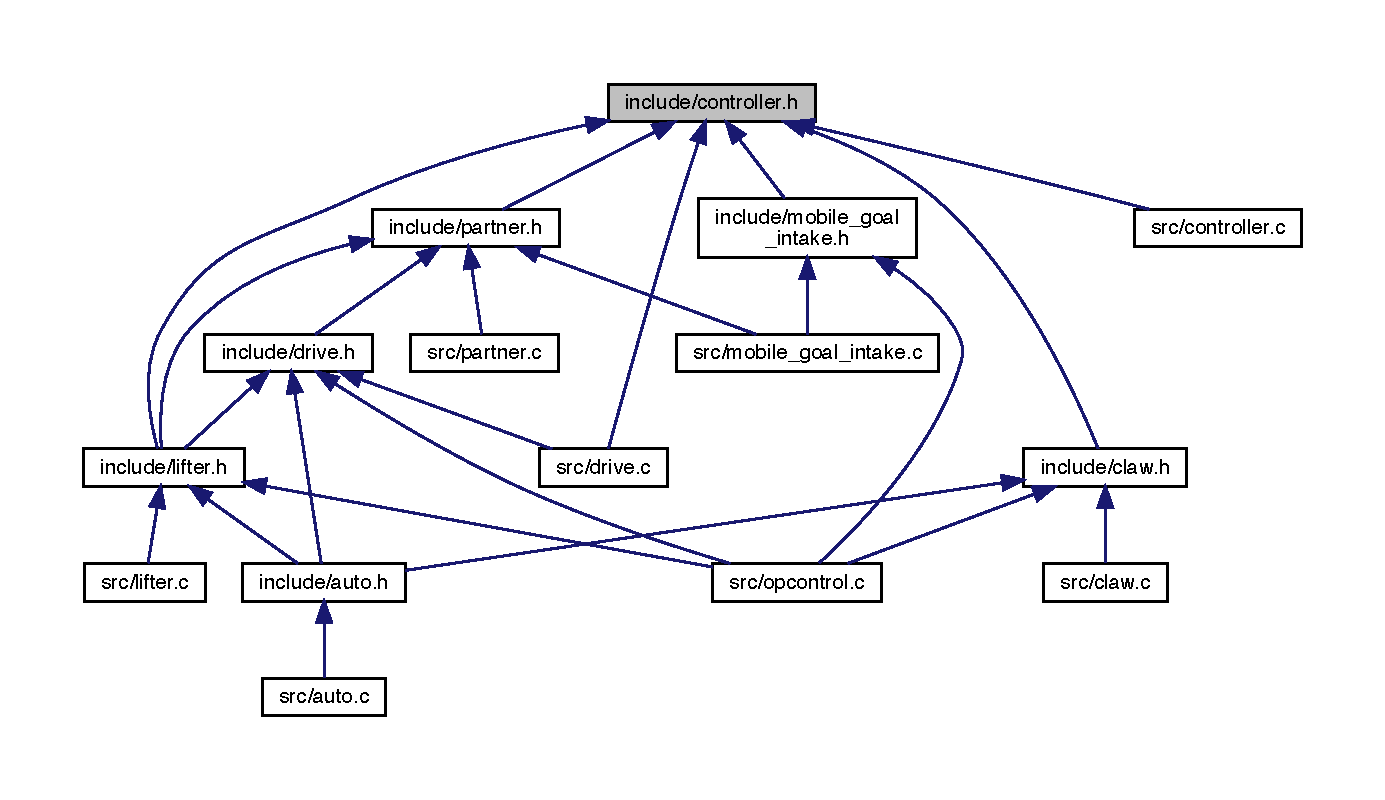
\includegraphics[width=350pt]{controller_8h__dep__incl}
\end{center}
\end{figure}
\subsection*{Macros}
\begin{DoxyCompactItemize}
\item 
\#define \textbf{ L\+E\+F\+T\+\_\+\+B\+U\+M\+P\+E\+RS}~6
\item 
\#define \textbf{ L\+E\+F\+T\+\_\+\+B\+U\+T\+T\+O\+NS}~7
\item 
\#define \textbf{ L\+E\+F\+T\+\_\+\+J\+O\+Y\+\_\+X}~4
\begin{DoxyCompactList}\small\item\em the left x joystick on controller \end{DoxyCompactList}\item 
\#define \textbf{ L\+E\+F\+T\+\_\+\+J\+O\+Y\+\_\+Y}~3
\begin{DoxyCompactList}\small\item\em the left y joystick on controller \end{DoxyCompactList}\item 
\#define \textbf{ M\+A\+S\+T\+ER}~1
\begin{DoxyCompactList}\small\item\em the master controller \end{DoxyCompactList}\item 
\#define \textbf{ P\+A\+R\+T\+N\+ER}~2
\begin{DoxyCompactList}\small\item\em the slave/partner controller \end{DoxyCompactList}\item 
\#define \textbf{ R\+I\+G\+H\+T\+\_\+\+B\+U\+M\+P\+E\+RS}~5
\item 
\#define \textbf{ R\+I\+G\+H\+T\+\_\+\+B\+U\+T\+T\+O\+NS}~8
\item 
\#define \textbf{ R\+I\+G\+H\+T\+\_\+\+J\+O\+Y\+\_\+X}~1
\begin{DoxyCompactList}\small\item\em the right x joystick on controller \end{DoxyCompactList}\item 
\#define \textbf{ R\+I\+G\+H\+T\+\_\+\+J\+O\+Y\+\_\+Y}~2
\begin{DoxyCompactList}\small\item\em the right y joystick on controller \end{DoxyCompactList}\end{DoxyCompactItemize}
\subsection*{Enumerations}
\begin{DoxyCompactItemize}
\item 
enum \textbf{ joystick} \{ \textbf{ R\+I\+G\+H\+T\+\_\+\+J\+OY}, 
\textbf{ L\+E\+F\+T\+\_\+\+J\+OY}
 \}\begin{DoxyCompactList}\small\item\em Represents a joystick on the controller. \end{DoxyCompactList}
\end{DoxyCompactItemize}
\subsection*{Functions}
\begin{DoxyCompactItemize}
\item 
struct \textbf{ cord} \textbf{ get\+\_\+joystick\+\_\+cord} (enum \textbf{ joystick} \textbf{ side}, int controller)
\begin{DoxyCompactList}\small\item\em Gets the location of a joystick on the controller. \end{DoxyCompactList}\end{DoxyCompactItemize}


\subsection{Detailed Description}
controller definitions, macros and functions to assist with usig the vex controllers. 

\begin{DoxyAuthor}{Author}
Chris Jerrett, Christian Desimone 
\end{DoxyAuthor}
\begin{DoxyDate}{Date}
9/9/2017 
\end{DoxyDate}


Definition in file \textbf{ controller.\+h}.



\subsection{Macro Definition Documentation}
\mbox{\label{controller_8h_ad61eb6d28a76985afb8d39ef925541bb}} 
\index{controller.\+h@{controller.\+h}!L\+E\+F\+T\+\_\+\+B\+U\+M\+P\+E\+RS@{L\+E\+F\+T\+\_\+\+B\+U\+M\+P\+E\+RS}}
\index{L\+E\+F\+T\+\_\+\+B\+U\+M\+P\+E\+RS@{L\+E\+F\+T\+\_\+\+B\+U\+M\+P\+E\+RS}!controller.\+h@{controller.\+h}}
\subsubsection{L\+E\+F\+T\+\_\+\+B\+U\+M\+P\+E\+RS}
{\footnotesize\ttfamily \#define L\+E\+F\+T\+\_\+\+B\+U\+M\+P\+E\+RS~6}



Definition at line \textbf{ 18} of file \textbf{ controller.\+h}.

\mbox{\label{controller_8h_a9b885de9f143efd0c862ceb054256536}} 
\index{controller.\+h@{controller.\+h}!L\+E\+F\+T\+\_\+\+B\+U\+T\+T\+O\+NS@{L\+E\+F\+T\+\_\+\+B\+U\+T\+T\+O\+NS}}
\index{L\+E\+F\+T\+\_\+\+B\+U\+T\+T\+O\+NS@{L\+E\+F\+T\+\_\+\+B\+U\+T\+T\+O\+NS}!controller.\+h@{controller.\+h}}
\subsubsection{L\+E\+F\+T\+\_\+\+B\+U\+T\+T\+O\+NS}
{\footnotesize\ttfamily \#define L\+E\+F\+T\+\_\+\+B\+U\+T\+T\+O\+NS~7}



Definition at line \textbf{ 16} of file \textbf{ controller.\+h}.

\mbox{\label{controller_8h_ac055a23829dc64aa20b8e2e1bcfbf316}} 
\index{controller.\+h@{controller.\+h}!L\+E\+F\+T\+\_\+\+J\+O\+Y\+\_\+X@{L\+E\+F\+T\+\_\+\+J\+O\+Y\+\_\+X}}
\index{L\+E\+F\+T\+\_\+\+J\+O\+Y\+\_\+X@{L\+E\+F\+T\+\_\+\+J\+O\+Y\+\_\+X}!controller.\+h@{controller.\+h}}
\subsubsection{L\+E\+F\+T\+\_\+\+J\+O\+Y\+\_\+X}
{\footnotesize\ttfamily \#define L\+E\+F\+T\+\_\+\+J\+O\+Y\+\_\+X~4}



the left x joystick on controller 

\begin{DoxyDate}{Date}
9/1/2017 
\end{DoxyDate}
\begin{DoxyAuthor}{Author}
Chris Jerrett 
\end{DoxyAuthor}


Definition at line \textbf{ 53} of file \textbf{ controller.\+h}.



Referenced by \textbf{ get\+\_\+joystick\+\_\+cord()}.

\mbox{\label{controller_8h_ae0a2b64db5fc4f4bf4b169185be93db3}} 
\index{controller.\+h@{controller.\+h}!L\+E\+F\+T\+\_\+\+J\+O\+Y\+\_\+Y@{L\+E\+F\+T\+\_\+\+J\+O\+Y\+\_\+Y}}
\index{L\+E\+F\+T\+\_\+\+J\+O\+Y\+\_\+Y@{L\+E\+F\+T\+\_\+\+J\+O\+Y\+\_\+Y}!controller.\+h@{controller.\+h}}
\subsubsection{L\+E\+F\+T\+\_\+\+J\+O\+Y\+\_\+Y}
{\footnotesize\ttfamily \#define L\+E\+F\+T\+\_\+\+J\+O\+Y\+\_\+Y~3}



the left y joystick on controller 

\begin{DoxyDate}{Date}
9/1/2017 
\end{DoxyDate}
\begin{DoxyAuthor}{Author}
Chris Jerrett 
\end{DoxyAuthor}


Definition at line \textbf{ 60} of file \textbf{ controller.\+h}.



Referenced by \textbf{ get\+\_\+joystick\+\_\+cord()}.

\mbox{\label{controller_8h_a3fa2d3bf1901157f734a584d47b25d8b}} 
\index{controller.\+h@{controller.\+h}!M\+A\+S\+T\+ER@{M\+A\+S\+T\+ER}}
\index{M\+A\+S\+T\+ER@{M\+A\+S\+T\+ER}!controller.\+h@{controller.\+h}}
\subsubsection{M\+A\+S\+T\+ER}
{\footnotesize\ttfamily \#define M\+A\+S\+T\+ER~1}



the master controller 

\begin{DoxyDate}{Date}
9/1/2017 
\end{DoxyDate}
\begin{DoxyAuthor}{Author}
Chris Jerrett 
\end{DoxyAuthor}


Definition at line \textbf{ 25} of file \textbf{ controller.\+h}.



Referenced by \textbf{ update\+\_\+drive\+\_\+motors()}, and \textbf{ update\+Intake()}.

\mbox{\label{controller_8h_a136e64cf351535da81cacb6a546cade6}} 
\index{controller.\+h@{controller.\+h}!P\+A\+R\+T\+N\+ER@{P\+A\+R\+T\+N\+ER}}
\index{P\+A\+R\+T\+N\+ER@{P\+A\+R\+T\+N\+ER}!controller.\+h@{controller.\+h}}
\subsubsection{P\+A\+R\+T\+N\+ER}
{\footnotesize\ttfamily \#define P\+A\+R\+T\+N\+ER~2}



the slave/partner controller 

\begin{DoxyDate}{Date}
9/1/2017 
\end{DoxyDate}
\begin{DoxyAuthor}{Author}
Chris Jerrett 
\end{DoxyAuthor}


Definition at line \textbf{ 32} of file \textbf{ controller.\+h}.



Referenced by \textbf{ update\+\_\+control()}, \textbf{ update\+\_\+drive\+\_\+motors()}, and \textbf{ update\+Intake()}.

\mbox{\label{controller_8h_a635896b08789914290171051d1b82465}} 
\index{controller.\+h@{controller.\+h}!R\+I\+G\+H\+T\+\_\+\+B\+U\+M\+P\+E\+RS@{R\+I\+G\+H\+T\+\_\+\+B\+U\+M\+P\+E\+RS}}
\index{R\+I\+G\+H\+T\+\_\+\+B\+U\+M\+P\+E\+RS@{R\+I\+G\+H\+T\+\_\+\+B\+U\+M\+P\+E\+RS}!controller.\+h@{controller.\+h}}
\subsubsection{R\+I\+G\+H\+T\+\_\+\+B\+U\+M\+P\+E\+RS}
{\footnotesize\ttfamily \#define R\+I\+G\+H\+T\+\_\+\+B\+U\+M\+P\+E\+RS~5}



Definition at line \textbf{ 17} of file \textbf{ controller.\+h}.

\mbox{\label{controller_8h_a68881b6085c880930037b20764fe5aee}} 
\index{controller.\+h@{controller.\+h}!R\+I\+G\+H\+T\+\_\+\+B\+U\+T\+T\+O\+NS@{R\+I\+G\+H\+T\+\_\+\+B\+U\+T\+T\+O\+NS}}
\index{R\+I\+G\+H\+T\+\_\+\+B\+U\+T\+T\+O\+NS@{R\+I\+G\+H\+T\+\_\+\+B\+U\+T\+T\+O\+NS}!controller.\+h@{controller.\+h}}
\subsubsection{R\+I\+G\+H\+T\+\_\+\+B\+U\+T\+T\+O\+NS}
{\footnotesize\ttfamily \#define R\+I\+G\+H\+T\+\_\+\+B\+U\+T\+T\+O\+NS~8}



Definition at line \textbf{ 15} of file \textbf{ controller.\+h}.

\mbox{\label{controller_8h_ad74f84aad465437cc1e0f914dbd6fab5}} 
\index{controller.\+h@{controller.\+h}!R\+I\+G\+H\+T\+\_\+\+J\+O\+Y\+\_\+X@{R\+I\+G\+H\+T\+\_\+\+J\+O\+Y\+\_\+X}}
\index{R\+I\+G\+H\+T\+\_\+\+J\+O\+Y\+\_\+X@{R\+I\+G\+H\+T\+\_\+\+J\+O\+Y\+\_\+X}!controller.\+h@{controller.\+h}}
\subsubsection{R\+I\+G\+H\+T\+\_\+\+J\+O\+Y\+\_\+X}
{\footnotesize\ttfamily \#define R\+I\+G\+H\+T\+\_\+\+J\+O\+Y\+\_\+X~1}



the right x joystick on controller 

\begin{DoxyDate}{Date}
9/1/2017 
\end{DoxyDate}
\begin{DoxyAuthor}{Author}
Chris Jerrett 
\end{DoxyAuthor}


Definition at line \textbf{ 39} of file \textbf{ controller.\+h}.



Referenced by \textbf{ get\+\_\+joystick\+\_\+cord()}.

\mbox{\label{controller_8h_a99457bf9dee795334411ea77f0858b16}} 
\index{controller.\+h@{controller.\+h}!R\+I\+G\+H\+T\+\_\+\+J\+O\+Y\+\_\+Y@{R\+I\+G\+H\+T\+\_\+\+J\+O\+Y\+\_\+Y}}
\index{R\+I\+G\+H\+T\+\_\+\+J\+O\+Y\+\_\+Y@{R\+I\+G\+H\+T\+\_\+\+J\+O\+Y\+\_\+Y}!controller.\+h@{controller.\+h}}
\subsubsection{R\+I\+G\+H\+T\+\_\+\+J\+O\+Y\+\_\+Y}
{\footnotesize\ttfamily \#define R\+I\+G\+H\+T\+\_\+\+J\+O\+Y\+\_\+Y~2}



the right y joystick on controller 

\begin{DoxyDate}{Date}
9/1/2017 
\end{DoxyDate}
\begin{DoxyAuthor}{Author}
Chris Jerrett 
\end{DoxyAuthor}


Definition at line \textbf{ 46} of file \textbf{ controller.\+h}.



Referenced by \textbf{ get\+\_\+joystick\+\_\+cord()}.



\subsection{Enumeration Type Documentation}
\mbox{\label{controller_8h_ac365c9e892abe4a1b85ae8f56a4eae5a}} 
\index{controller.\+h@{controller.\+h}!joystick@{joystick}}
\index{joystick@{joystick}!controller.\+h@{controller.\+h}}
\subsubsection{joystick}
{\footnotesize\ttfamily enum \textbf{ joystick}}



Represents a joystick on the controller. 

\begin{DoxyDate}{Date}
9/10/2017 
\end{DoxyDate}
\begin{DoxyAuthor}{Author}
Chris Jerrett 
\end{DoxyAuthor}
\begin{DoxyEnumFields}{Enumerator}
\raisebox{\heightof{T}}[0pt][0pt]{\index{R\+I\+G\+H\+T\+\_\+\+J\+OY@{R\+I\+G\+H\+T\+\_\+\+J\+OY}!controller.\+h@{controller.\+h}}\index{controller.\+h@{controller.\+h}!R\+I\+G\+H\+T\+\_\+\+J\+OY@{R\+I\+G\+H\+T\+\_\+\+J\+OY}}}\mbox{\label{controller_8h_ac365c9e892abe4a1b85ae8f56a4eae5aae08a2d362c677f96f72d93047513cafe}} 
R\+I\+G\+H\+T\+\_\+\+J\+OY&The right joystick \\
\hline

\raisebox{\heightof{T}}[0pt][0pt]{\index{L\+E\+F\+T\+\_\+\+J\+OY@{L\+E\+F\+T\+\_\+\+J\+OY}!controller.\+h@{controller.\+h}}\index{controller.\+h@{controller.\+h}!L\+E\+F\+T\+\_\+\+J\+OY@{L\+E\+F\+T\+\_\+\+J\+OY}}}\mbox{\label{controller_8h_ac365c9e892abe4a1b85ae8f56a4eae5aaf822d7888862e67a3c624775b85c50a9}} 
L\+E\+F\+T\+\_\+\+J\+OY&The left joystick \\
\hline

\end{DoxyEnumFields}


Definition at line \textbf{ 67} of file \textbf{ controller.\+h}.


\begin{DoxyCode}
00067               \{
00069   RIGHT_JOY,
00071   LEFT_JOY,
00072 \};
\end{DoxyCode}


\subsection{Function Documentation}
\mbox{\label{controller_8h_a0ce0176099c0bb15ad8c36123222059d}} 
\index{controller.\+h@{controller.\+h}!get\+\_\+joystick\+\_\+cord@{get\+\_\+joystick\+\_\+cord}}
\index{get\+\_\+joystick\+\_\+cord@{get\+\_\+joystick\+\_\+cord}!controller.\+h@{controller.\+h}}
\subsubsection{get\+\_\+joystick\+\_\+cord()}
{\footnotesize\ttfamily struct \textbf{ cord} get\+\_\+joystick\+\_\+cord (\begin{DoxyParamCaption}\item[{enum \textbf{ joystick}}]{side,  }\item[{int}]{controller }\end{DoxyParamCaption})}



Gets the location of a joystick on the controller. 

\begin{DoxyAuthor}{Author}
Chris Jerrett 
\end{DoxyAuthor}


Definition at line \textbf{ 7} of file \textbf{ controller.\+c}.



References \textbf{ L\+E\+F\+T\+\_\+\+J\+O\+Y\+\_\+X}, \textbf{ L\+E\+F\+T\+\_\+\+J\+O\+Y\+\_\+Y}, \textbf{ R\+I\+G\+H\+T\+\_\+\+J\+OY}, \textbf{ R\+I\+G\+H\+T\+\_\+\+J\+O\+Y\+\_\+X}, \textbf{ R\+I\+G\+H\+T\+\_\+\+J\+O\+Y\+\_\+Y}, \textbf{ cord\+::x}, and \textbf{ cord\+::y}.


\begin{DoxyCode}
00007                                                                   \{
00008   \textcolor{keywordtype}{int} x;
00009   \textcolor{keywordtype}{int} y;
00010   \textcolor{comment}{//Get the joystick value for either the right or left,}
00011   \textcolor{comment}{//depending on the mode}
00012   \textcolor{keywordflow}{if}(side == RIGHT_JOY) \{
00013     y = joystickGetAnalog(controller, RIGHT_JOY_X);
00014     x = joystickGetAnalog(controller, RIGHT_JOY_Y);
00015   \} \textcolor{keywordflow}{else} \{
00016     y = joystickGetAnalog(controller, LEFT_JOY_X);
00017     x = joystickGetAnalog(controller, LEFT_JOY_Y);
00018   \}
00019   \textcolor{comment}{//Define a coordinate for the joystick value}
00020   \textcolor{keyword}{struct }cord c;
00021   c.x = x;
00022   c.y = y;
00023   \textcolor{keywordflow}{return} c;
00024 \}
\end{DoxyCode}

\subsection{controller.\+h}
\label{controller_8h_source}\index{include/controller.\+h@{include/controller.\+h}}

\begin{DoxyCode}
00001 
00009 \textcolor{preprocessor}{#ifndef \_CONTROLLER\_H\_}
00010 \textcolor{preprocessor}{#define \_CONTROLLER\_H\_}
00011 
00012 \textcolor{preprocessor}{#include "vmath.h"}
00013 \textcolor{preprocessor}{#include <API.h>}
00014 
00015 \textcolor{preprocessor}{#define RIGHT\_BUTTONS 8}
00016 \textcolor{preprocessor}{#define LEFT\_BUTTONS 7}
00017 \textcolor{preprocessor}{#define RIGHT\_BUMPERS 5}
00018 \textcolor{preprocessor}{#define LEFT\_BUMPERS 6}
00019 
00023 \textcolor{keyword}{typedef} \textcolor{keyword}{enum} \{
00024   JOY1_5D = 0,
00025   JOY1_5U = 1,
00026   JOY1_6D = 2,
00027   JOY1_6U = 3,
00028   JOY1_7U = 4,
00029   JOY1_7L = 5,
00030   JOY1_7R = 6,
00031   JOY1_7D = 7,
00032   JOY1_8U = 8,
00033   JOY1_8L = 9,
00034   JOY1_8R = 10,
00035   JOY1_8D = 11,
00036 
00037   JOY2_5D = 12,
00038   JOY2_5U = 13,
00039   JOY2_6D = 14,
00040   JOY2_6U = 15,
00041   JOY2_7U = 16,
00042   JOY2_7L = 17,
00043   JOY2_7R = 18,
00044   JOY2_7D = 19,
00045   JOY2_8U = 20,
00046   JOY2_8L = 21,
00047   JOY2_8R = 22,
00048   JOY2_8D = 23,
00049 
00050   LCD_LEFT = 24,
00051   LCD_CENT = 25,
00052   LCD_RIGHT = 26
00053 \} button_t;
00054 
00060 \textcolor{preprocessor}{#define MASTER 1}
00061 
00067 \textcolor{preprocessor}{#define PARTNER 2}
00068 
00074 \textcolor{preprocessor}{#define RIGHT\_JOY\_X 1}
00075 
00081 \textcolor{preprocessor}{#define RIGHT\_JOY\_Y 2}
00082 
00088 \textcolor{preprocessor}{#define LEFT\_JOY\_X 4}
00089 
00095 \textcolor{preprocessor}{#define LEFT\_JOY\_Y 3}
00096 
00102 \textcolor{keyword}{enum} joystick \{
00104   RIGHT_JOY,
00106   LEFT_JOY,
00107 \};
00108 
00113 \textcolor{keyword}{struct }cord get_joystick_cord(enum joystick side, int controller);
00114 
00115 \textcolor{preprocessor}{#endif}
\end{DoxyCode}

\subsection{include/drive.h File Reference}
\label{drive_8h}\index{include/drive.\+h@{include/drive.\+h}}


Drive base definitions and enumerations.  


{\ttfamily \#include $<$A\+P\+I.\+h$>$}\newline
{\ttfamily \#include \char`\"{}partner.\+h\char`\"{}}\newline
Include dependency graph for drive.\+h\+:\nopagebreak
\begin{figure}[H]
\begin{center}
\leavevmode
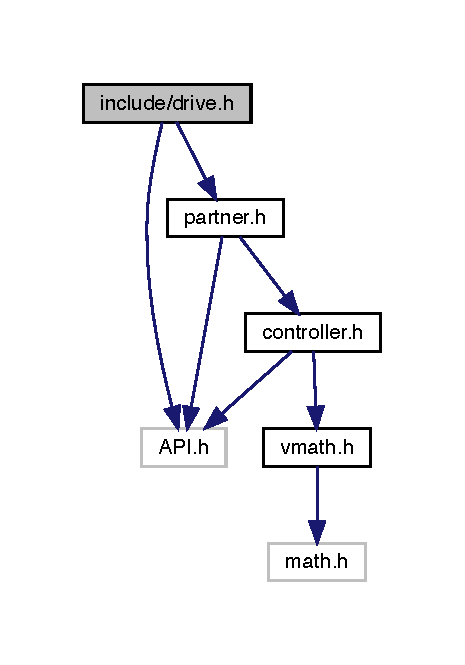
\includegraphics[width=350pt]{drive_8h__incl}
\end{center}
\end{figure}
This graph shows which files directly or indirectly include this file\+:\nopagebreak
\begin{figure}[H]
\begin{center}
\leavevmode
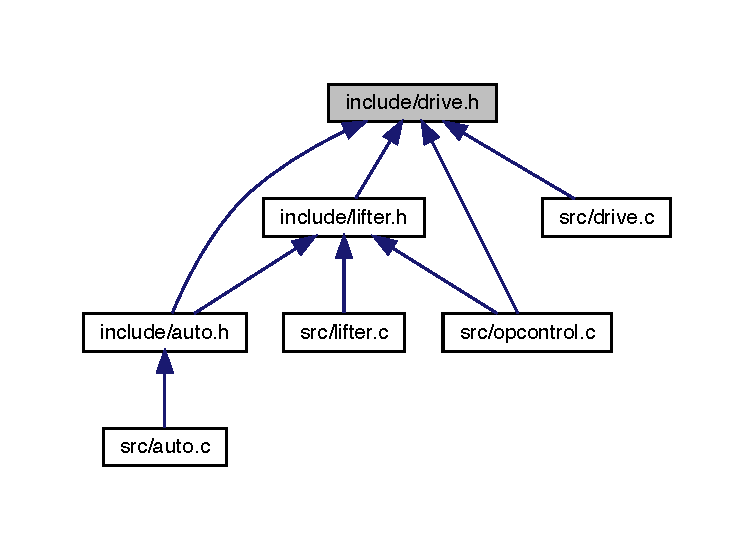
\includegraphics[width=350pt]{drive_8h__dep__incl}
\end{center}
\end{figure}
\subsubsection*{Macros}
\begin{DoxyCompactItemize}
\item 
\#define \textbf{ T\+H\+R\+E\+S\+H\+O\+LD}~10
\begin{DoxyCompactList}\small\item\em The dead spot on the controller to avoid running motors at low speeds. \end{DoxyCompactList}\end{DoxyCompactItemize}
\subsubsection*{Typedefs}
\begin{DoxyCompactItemize}
\item 
typedef enum \textbf{ side} \textbf{ side\+\_\+t}
\begin{DoxyCompactList}\small\item\em enumeration indication side of the robot. \end{DoxyCompactList}\end{DoxyCompactItemize}
\subsubsection*{Enumerations}
\begin{DoxyCompactItemize}
\item 
enum \textbf{ side} \{ \textbf{ L\+E\+FT}, 
\textbf{ B\+O\+TH}, 
\textbf{ R\+I\+G\+HT}
 \}\begin{DoxyCompactList}\small\item\em enumeration indication side of the robot. \end{DoxyCompactList}
\end{DoxyCompactItemize}
\subsubsection*{Functions}
\begin{DoxyCompactItemize}
\item 
void \textbf{ set\+\_\+side\+\_\+speed} (\textbf{ side\+\_\+t} \textbf{ side}, int speed)
\begin{DoxyCompactList}\small\item\em sets the speed of one side of the robot. \end{DoxyCompactList}\item 
void \textbf{ set\+Thresh} (int t)
\begin{DoxyCompactList}\small\item\em Sets the deadzone threshhold on the drive. \end{DoxyCompactList}\item 
void \textbf{ update\+\_\+drive\+\_\+motors} ()
\begin{DoxyCompactList}\small\item\em Updates the drive motors during teleop. \end{DoxyCompactList}\end{DoxyCompactItemize}


\subsubsection{Detailed Description}
Drive base definitions and enumerations. 

\begin{DoxyAuthor}{Author}
Chris Jerrett 
\end{DoxyAuthor}
\begin{DoxyDate}{Date}
9/9/2017 
\end{DoxyDate}


Definition in file \textbf{ drive.\+h}.



\subsubsection{Macro Definition Documentation}
\mbox{\label{drive_8h_a4679d8ea8690999a6c6c7c0cb245c879}} 
\index{drive.\+h@{drive.\+h}!T\+H\+R\+E\+S\+H\+O\+LD@{T\+H\+R\+E\+S\+H\+O\+LD}}
\index{T\+H\+R\+E\+S\+H\+O\+LD@{T\+H\+R\+E\+S\+H\+O\+LD}!drive.\+h@{drive.\+h}}
\paragraph{T\+H\+R\+E\+S\+H\+O\+LD}
{\footnotesize\ttfamily \#define T\+H\+R\+E\+S\+H\+O\+LD~10}



The dead spot on the controller to avoid running motors at low speeds. 



Definition at line \textbf{ 18} of file \textbf{ drive.\+h}.



Referenced by \textbf{ joystick\+Exp()}, and \textbf{ update\+\_\+lifter()}.



\subsubsection{Typedef Documentation}
\mbox{\label{drive_8h_a9df2afd2f1acb97019655e5e730609c7}} 
\index{drive.\+h@{drive.\+h}!side\+\_\+t@{side\+\_\+t}}
\index{side\+\_\+t@{side\+\_\+t}!drive.\+h@{drive.\+h}}
\paragraph{side\+\_\+t}
{\footnotesize\ttfamily typedef enum \textbf{ side}  \textbf{ side\+\_\+t}}



enumeration indication side of the robot. 

\begin{DoxyAuthor}{Author}
Christian Desimone 
\end{DoxyAuthor}
\begin{DoxyDate}{Date}
9/7/2017 Side can be right, both of left. Contained in side typedef, so enum is unnecessary. 
\end{DoxyDate}


\subsubsection{Enumeration Type Documentation}
\mbox{\label{drive_8h_afc015eff6557e84151d2e53b94375445}} 
\index{drive.\+h@{drive.\+h}!side@{side}}
\index{side@{side}!drive.\+h@{drive.\+h}}
\paragraph{side}
{\footnotesize\ttfamily enum \textbf{ side}}



enumeration indication side of the robot. 

\begin{DoxyAuthor}{Author}
Christian Desimone 
\end{DoxyAuthor}
\begin{DoxyDate}{Date}
9/7/2017 Side can be right, both of left. Contained in side typedef, so enum is unnecessary. 
\end{DoxyDate}
\begin{DoxyEnumFields}{Enumerator}
\raisebox{\heightof{T}}[0pt][0pt]{\index{L\+E\+FT@{L\+E\+FT}!drive.\+h@{drive.\+h}}\index{drive.\+h@{drive.\+h}!L\+E\+FT@{L\+E\+FT}}}\mbox{\label{drive_8h_afc015eff6557e84151d2e53b94375445adb45120aafd37a973140edee24708065}} 
L\+E\+FT&\\
\hline

\raisebox{\heightof{T}}[0pt][0pt]{\index{B\+O\+TH@{B\+O\+TH}!drive.\+h@{drive.\+h}}\index{drive.\+h@{drive.\+h}!B\+O\+TH@{B\+O\+TH}}}\mbox{\label{drive_8h_afc015eff6557e84151d2e53b94375445a627abe5a430420baf29ebe1940a7f2fb}} 
B\+O\+TH&\\
\hline

\raisebox{\heightof{T}}[0pt][0pt]{\index{R\+I\+G\+HT@{R\+I\+G\+HT}!drive.\+h@{drive.\+h}}\index{drive.\+h@{drive.\+h}!R\+I\+G\+HT@{R\+I\+G\+HT}}}\mbox{\label{drive_8h_afc015eff6557e84151d2e53b94375445aec8379af7490bb9eaaf579cf17876f38}} 
R\+I\+G\+HT&\\
\hline

\end{DoxyEnumFields}


Definition at line \textbf{ 26} of file \textbf{ drive.\+h}.


\begin{DoxyCode}
00026                  \{
00027   LEFT,
00028   BOTH,
00029   RIGHT
00030 \} side_t;
\end{DoxyCode}


\subsubsection{Function Documentation}
\mbox{\label{drive_8h_a8df41fd50094c065eedc81fc5e6595d1}} 
\index{drive.\+h@{drive.\+h}!set\+\_\+side\+\_\+speed@{set\+\_\+side\+\_\+speed}}
\index{set\+\_\+side\+\_\+speed@{set\+\_\+side\+\_\+speed}!drive.\+h@{drive.\+h}}
\paragraph{set\+\_\+side\+\_\+speed()}
{\footnotesize\ttfamily void set\+\_\+side\+\_\+speed (\begin{DoxyParamCaption}\item[{\textbf{ side\+\_\+t}}]{side,  }\item[{int}]{speed }\end{DoxyParamCaption})}



sets the speed of one side of the robot. 

\begin{DoxyAuthor}{Author}
Christian Desimone 
\end{DoxyAuthor}

\begin{DoxyParams}{Parameters}
{\em side} & a side enum which indicates the size. \\
\hline
{\em speed} & the speed of the side. Can range from -\/127 -\/ 127 negative being back and positive forwards \\
\hline
\end{DoxyParams}


Definition at line \textbf{ 68} of file \textbf{ drive.\+c}.



References \textbf{ B\+O\+TH}, \textbf{ L\+E\+FT}, \textbf{ M\+O\+T\+O\+R\+\_\+\+B\+A\+C\+K\+\_\+\+L\+E\+FT}, \textbf{ M\+O\+T\+O\+R\+\_\+\+B\+A\+C\+K\+\_\+\+R\+I\+G\+HT}, \textbf{ M\+O\+T\+O\+R\+\_\+\+F\+R\+O\+N\+T\+\_\+\+L\+E\+FT}, \textbf{ M\+O\+T\+O\+R\+\_\+\+F\+R\+O\+N\+T\+\_\+\+R\+I\+G\+HT}, \textbf{ M\+O\+T\+O\+R\+\_\+\+M\+I\+D\+D\+L\+E\+\_\+\+L\+E\+FT}, \textbf{ M\+O\+T\+O\+R\+\_\+\+M\+I\+D\+D\+L\+E\+\_\+\+R\+I\+G\+HT}, \textbf{ R\+I\+G\+HT}, and \textbf{ set\+\_\+motor\+\_\+slew()}.



Referenced by \textbf{ autonomous()}, and \textbf{ update\+\_\+drive\+\_\+motors()}.


\begin{DoxyCode}
00068                                            \{
00069   \textcolor{keywordflow}{if}(side == RIGHT || side == BOTH)\{
00070     set_motor_slew(MOTOR_BACK_RIGHT , -speed);
00071     set_motor_slew(MOTOR_FRONT_RIGHT, -speed);
00072     set_motor_slew(MOTOR_MIDDLE_RIGHT, -speed);
00073   \}
00074   \textcolor{keywordflow}{if}(side == LEFT || side == BOTH)\{
00075     set_motor_slew(MOTOR_BACK_LEFT, speed);
00076     set_motor_slew(MOTOR_MIDDLE_LEFT, speed);
00077     set_motor_slew(MOTOR_FRONT_LEFT, speed);
00078   \}
00079 \}
\end{DoxyCode}
Here is the call graph for this function\+:\nopagebreak
\begin{figure}[H]
\begin{center}
\leavevmode
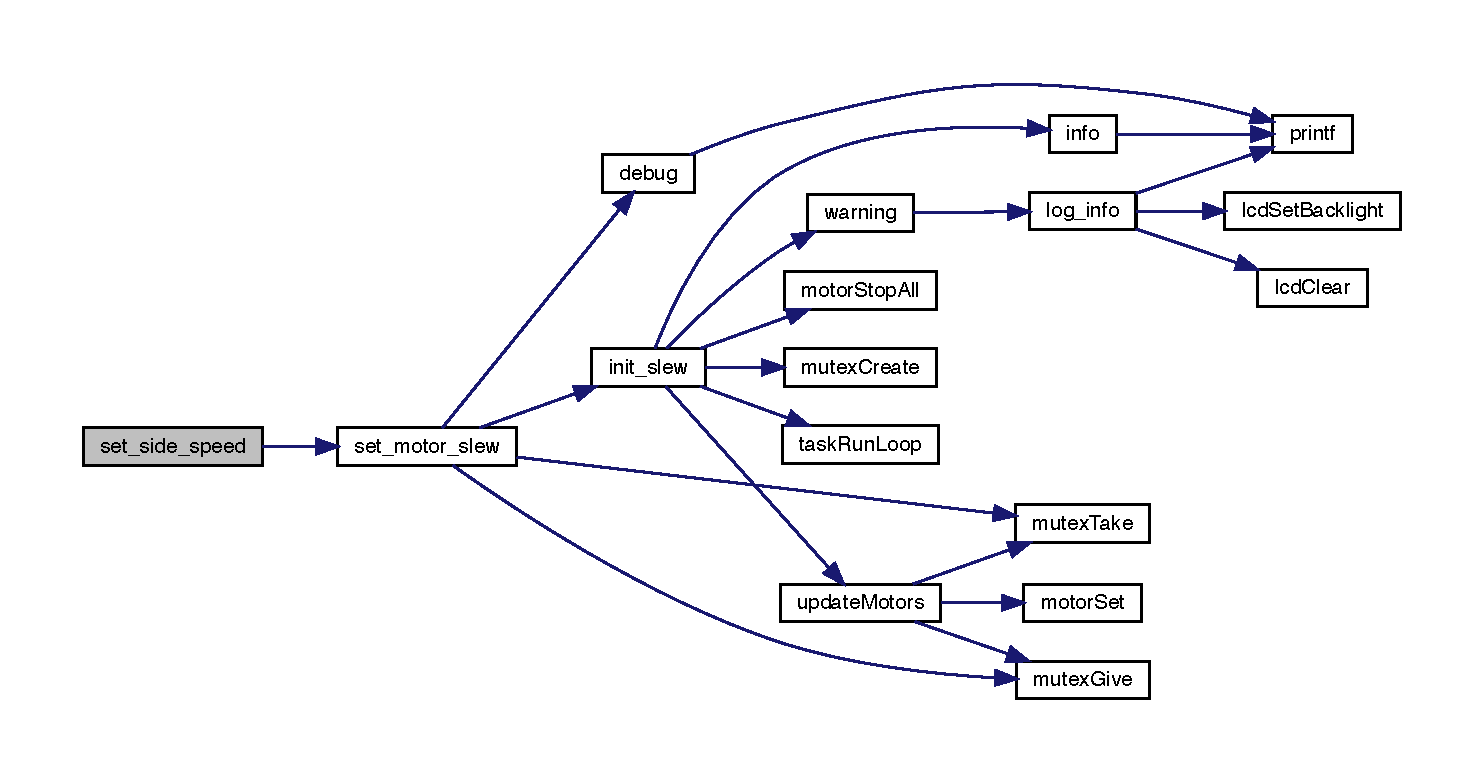
\includegraphics[width=350pt]{drive_8h_a8df41fd50094c065eedc81fc5e6595d1_cgraph}
\end{center}
\end{figure}
Here is the caller graph for this function\+:\nopagebreak
\begin{figure}[H]
\begin{center}
\leavevmode
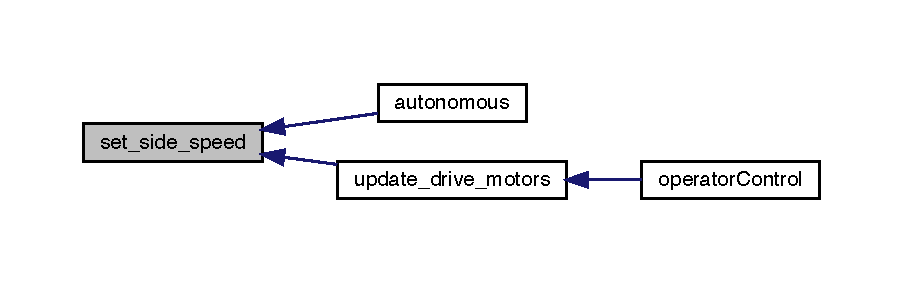
\includegraphics[width=350pt]{drive_8h_a8df41fd50094c065eedc81fc5e6595d1_icgraph}
\end{center}
\end{figure}
\mbox{\label{drive_8h_a53d6e35d53ec3e0b1b1c489d8203f204}} 
\index{drive.\+h@{drive.\+h}!set\+Thresh@{set\+Thresh}}
\index{set\+Thresh@{set\+Thresh}!drive.\+h@{drive.\+h}}
\paragraph{set\+Thresh()}
{\footnotesize\ttfamily void set\+Thresh (\begin{DoxyParamCaption}\item[{int}]{t }\end{DoxyParamCaption})}



Sets the deadzone threshhold on the drive. 

\begin{DoxyAuthor}{Author}
Chris Jerrett

Christian Desimone 
\end{DoxyAuthor}


Definition at line \textbf{ 25} of file \textbf{ drive.\+c}.



References \textbf{ thresh}.


\begin{DoxyCode}
00025                      \{
00026   thresh = t;
00027 \}
\end{DoxyCode}
\mbox{\label{drive_8h_a8224a4626a934d30ed587671b7004bf8}} 
\index{drive.\+h@{drive.\+h}!update\+\_\+drive\+\_\+motors@{update\+\_\+drive\+\_\+motors}}
\index{update\+\_\+drive\+\_\+motors@{update\+\_\+drive\+\_\+motors}!drive.\+h@{drive.\+h}}
\paragraph{update\+\_\+drive\+\_\+motors()}
{\footnotesize\ttfamily void update\+\_\+drive\+\_\+motors (\begin{DoxyParamCaption}{ }\end{DoxyParamCaption})}



Updates the drive motors during teleop. 

\begin{DoxyAuthor}{Author}
Christian Desimone 
\end{DoxyAuthor}
\begin{DoxyDate}{Date}
9/5/17 
\end{DoxyDate}


Definition at line \textbf{ 34} of file \textbf{ drive.\+c}.



References \textbf{ get\+\_\+mode()}, \textbf{ joystick\+Get\+Analog()}, \textbf{ L\+E\+FT}, \textbf{ M\+A\+S\+T\+ER}, \textbf{ P\+A\+R\+T\+N\+ER}, \textbf{ P\+A\+R\+T\+N\+E\+R\+\_\+\+C\+O\+N\+T\+R\+O\+L\+L\+E\+R\+\_\+\+M\+O\+DE}, \textbf{ R\+I\+G\+HT}, \textbf{ set\+\_\+side\+\_\+speed()}, \textbf{ thresh}, \textbf{ cord\+::x}, and \textbf{ cord\+::y}.



Referenced by \textbf{ operator\+Control()}.


\begin{DoxyCode}
00034                           \{
00035   \textcolor{comment}{//Get the joystick values from the controller}
00036   \textcolor{keywordtype}{int} x = 0;
00037   \textcolor{keywordtype}{int} y = 0;
00038   \textcolor{keywordflow}{if}(get_mode() == PARTNER_CONTROLLER_MODE) \{
00039     x = (joystickGetAnalog(PARTNER, 3));
00040     y = (joystickGetAnalog(PARTNER, 1));
00041   \} \textcolor{keywordflow}{else} \{
00042     x = -(joystickGetAnalog(MASTER, 3));
00043     y = (joystickGetAnalog(MASTER, 1));
00044   \}
00045   \textcolor{comment}{//Make sure the joystick values are significant enough to change the motors}
00046   \textcolor{keywordflow}{if}(x < thresh && x > -thresh)\{
00047     x = 0;
00048   \}
00049   \textcolor{keywordflow}{if}(y < thresh && y > -thresh)\{
00050     y = 0;
00051   \}
00052   \textcolor{comment}{//Create motor values for the left and right from the x and y of the joystick}
00053   \textcolor{keywordtype}{int} r = (x + y);
00054   \textcolor{keywordtype}{int} l = -(x - y);
00055 
00056   \textcolor{comment}{//Set the drive motors}
00057   set_side_speed(LEFT, l);
00058   set_side_speed(RIGHT, -r);
00059 
00060 \}
\end{DoxyCode}
Here is the call graph for this function\+:\nopagebreak
\begin{figure}[H]
\begin{center}
\leavevmode
\includegraphics[width=350pt]{drive_8h_a8224a4626a934d30ed587671b7004bf8_cgraph}
\end{center}
\end{figure}
Here is the caller graph for this function\+:\nopagebreak
\begin{figure}[H]
\begin{center}
\leavevmode
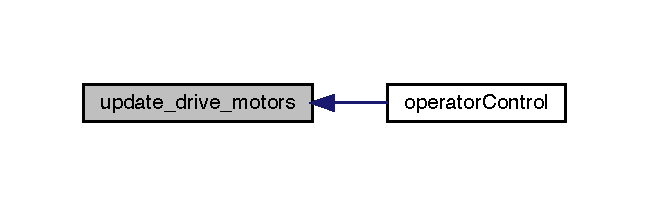
\includegraphics[width=311pt]{drive_8h_a8224a4626a934d30ed587671b7004bf8_icgraph}
\end{center}
\end{figure}

\section{drive.\+h}
\label{drive_8h_source}\index{include/drive.\+h@{include/drive.\+h}}

\begin{DoxyCode}
00001 
00008 \textcolor{preprocessor}{#ifndef \_DRIVE\_H\_}
00009 \textcolor{preprocessor}{#define \_DRIVE\_H\_}
00010 
00011 \textcolor{preprocessor}{#include <API.h>}
00012 \textcolor{preprocessor}{#include "partner.h"}
00013 
00018 \textcolor{preprocessor}{#define THRESHOLD 10}
00019 
00026 \textcolor{keyword}{typedef} \textcolor{keyword}{enum} side\{
00027   LEFT,
00028   BOTH,
00029   RIGHT
00030 \} side_t;
00031 
00038 \textcolor{keywordtype}{void} set_side_speed(side_t side, \textcolor{keywordtype}{int} speed);
00039 
00044 \textcolor{keywordtype}{void} setThresh(\textcolor{keywordtype}{int} t);
00045 
00051 \textcolor{keywordtype}{void} update_drive_motors();
00052 
00053 \textcolor{preprocessor}{#endif}
\end{DoxyCode}

\hypertarget{encoders_8h}{}\section{include/encoders.h File Reference}
\label{encoders_8h}\index{include/encoders.\+h@{include/encoders.\+h}}


wrapper around encoder functions  


{\ttfamily \#include $<$A\+P\+I.\+h$>$}\newline
\subsection*{Macros}
\begin{DoxyCompactItemize}
\item 
\#define \hyperlink{encoders_8h_a87db35d2735ef045f57d446b3bfe8d48}{I\+M\+E\+\_\+\+N\+U\+M\+B\+ER}~0
\begin{DoxyCompactList}\small\item\em The number of I\+M\+Es. This number is compared against the number detect in init\+\_\+encoders. \end{DoxyCompactList}\end{DoxyCompactItemize}
\subsection*{Functions}
\begin{DoxyCompactItemize}
\item 
int \hyperlink{encoders_8h_aed261dd4dae33a48c42f2e363c84760f}{get\+\_\+encoder\+\_\+ticks} (unsigned char address)
\begin{DoxyCompactList}\small\item\em Gets the encoder ticks since last reset. \end{DoxyCompactList}\item 
int \hyperlink{encoders_8h_a8e6b77703c5cf18e00709b052fb4bf22}{get\+\_\+encoder\+\_\+velocity} (unsigned char address)
\begin{DoxyCompactList}\small\item\em Gets the encoder reads. \end{DoxyCompactList}\item 
bool \hyperlink{encoders_8h_aa6ec1ca17e907babd52803ecba451cd3}{init\+\_\+encoders} ()
\begin{DoxyCompactList}\small\item\em Initializes all motor encoders. \end{DoxyCompactList}\end{DoxyCompactItemize}


\subsection{Detailed Description}
wrapper around encoder functions 

\begin{DoxyAuthor}{Author}
Chris Jerrett 
\end{DoxyAuthor}
\begin{DoxyDate}{Date}
9/9/2017 
\end{DoxyDate}


\subsection{Macro Definition Documentation}
\mbox{\Hypertarget{encoders_8h_a87db35d2735ef045f57d446b3bfe8d48}\label{encoders_8h_a87db35d2735ef045f57d446b3bfe8d48}} 
\index{encoders.\+h@{encoders.\+h}!I\+M\+E\+\_\+\+N\+U\+M\+B\+ER@{I\+M\+E\+\_\+\+N\+U\+M\+B\+ER}}
\index{I\+M\+E\+\_\+\+N\+U\+M\+B\+ER@{I\+M\+E\+\_\+\+N\+U\+M\+B\+ER}!encoders.\+h@{encoders.\+h}}
\subsubsection{\texorpdfstring{I\+M\+E\+\_\+\+N\+U\+M\+B\+ER}{IME\_NUMBER}}
{\footnotesize\ttfamily \#define I\+M\+E\+\_\+\+N\+U\+M\+B\+ER~0}



The number of I\+M\+Es. This number is compared against the number detect in init\+\_\+encoders. 

\begin{DoxySeeAlso}{See also}
\hyperlink{encoders_8h_aa6ec1ca17e907babd52803ecba451cd3}{init\+\_\+encoders()} 
\end{DoxySeeAlso}
\begin{DoxyAuthor}{Author}
Chris Jerrett 
\end{DoxyAuthor}
\begin{DoxyDate}{Date}
9/9/2017 
\end{DoxyDate}
\begin{DoxySeeAlso}{See also}
\hyperlink{encoders_8h_a87db35d2735ef045f57d446b3bfe8d48}{I\+M\+E\+\_\+\+N\+U\+M\+B\+ER} 
\end{DoxySeeAlso}


Definition at line 21 of file encoders.\+h.



Referenced by init\+\_\+encoders().



\subsection{Function Documentation}
\mbox{\Hypertarget{encoders_8h_aed261dd4dae33a48c42f2e363c84760f}\label{encoders_8h_aed261dd4dae33a48c42f2e363c84760f}} 
\index{encoders.\+h@{encoders.\+h}!get\+\_\+encoder\+\_\+ticks@{get\+\_\+encoder\+\_\+ticks}}
\index{get\+\_\+encoder\+\_\+ticks@{get\+\_\+encoder\+\_\+ticks}!encoders.\+h@{encoders.\+h}}
\subsubsection{\texorpdfstring{get\+\_\+encoder\+\_\+ticks()}{get\_encoder\_ticks()}}
{\footnotesize\ttfamily int get\+\_\+encoder\+\_\+ticks (\begin{DoxyParamCaption}\item[{unsigned char}]{address }\end{DoxyParamCaption})}



Gets the encoder ticks since last reset. 

\begin{DoxyAuthor}{Author}
Chris Jerrett 
\end{DoxyAuthor}
\begin{DoxyDate}{Date}
9/15/2017 
\end{DoxyDate}


Definition at line 12 of file encoders.\+c.


\begin{DoxyCode}
12                                              \{
13   \textcolor{keywordtype}{int} i = 0;
14   imeGet(address, &i);
15   \textcolor{keywordflow}{return} i;
16 \}
\end{DoxyCode}
\mbox{\Hypertarget{encoders_8h_a8e6b77703c5cf18e00709b052fb4bf22}\label{encoders_8h_a8e6b77703c5cf18e00709b052fb4bf22}} 
\index{encoders.\+h@{encoders.\+h}!get\+\_\+encoder\+\_\+velocity@{get\+\_\+encoder\+\_\+velocity}}
\index{get\+\_\+encoder\+\_\+velocity@{get\+\_\+encoder\+\_\+velocity}!encoders.\+h@{encoders.\+h}}
\subsubsection{\texorpdfstring{get\+\_\+encoder\+\_\+velocity()}{get\_encoder\_velocity()}}
{\footnotesize\ttfamily int get\+\_\+encoder\+\_\+velocity (\begin{DoxyParamCaption}\item[{unsigned char}]{address }\end{DoxyParamCaption})}



Gets the encoder reads. 

\begin{DoxyAuthor}{Author}
Chris Jerrett 
\end{DoxyAuthor}
\begin{DoxyDate}{Date}
9/15/2017 
\end{DoxyDate}


Definition at line 18 of file encoders.\+c.


\begin{DoxyCode}
18                                                 \{
19   \textcolor{keywordtype}{int} i = 0;
20   imeGetVelocity(address, &i);
21   \textcolor{keywordflow}{return} i;
22 \}
\end{DoxyCode}
\mbox{\Hypertarget{encoders_8h_aa6ec1ca17e907babd52803ecba451cd3}\label{encoders_8h_aa6ec1ca17e907babd52803ecba451cd3}} 
\index{encoders.\+h@{encoders.\+h}!init\+\_\+encoders@{init\+\_\+encoders}}
\index{init\+\_\+encoders@{init\+\_\+encoders}!encoders.\+h@{encoders.\+h}}
\subsubsection{\texorpdfstring{init\+\_\+encoders()}{init\_encoders()}}
{\footnotesize\ttfamily bool init\+\_\+encoders (\begin{DoxyParamCaption}{ }\end{DoxyParamCaption})}



Initializes all motor encoders. 

\begin{DoxyAuthor}{Author}
Chris Jerrett 
\end{DoxyAuthor}
\begin{DoxyDate}{Date}
9/9/2017 
\end{DoxyDate}
\begin{DoxySeeAlso}{See also}
\hyperlink{encoders_8h_a87db35d2735ef045f57d446b3bfe8d48}{I\+M\+E\+\_\+\+N\+U\+M\+B\+ER} 
\end{DoxySeeAlso}


Definition at line 4 of file encoders.\+c.



References I\+M\+E\+\_\+\+N\+U\+M\+B\+ER.



Referenced by initialize().


\begin{DoxyCode}
4                      \{
5 \textcolor{preprocessor}{  #ifdef IME\_NUMBER}
6   \textcolor{keywordflow}{return} imeInitializeAll() == \hyperlink{encoders_8h_a87db35d2735ef045f57d446b3bfe8d48}{IME\_NUMBER};
7 \textcolor{preprocessor}{  #else}
8   \textcolor{keywordflow}{return} imeInitializeAll();
9 \textcolor{preprocessor}{  #endif}
10 \}
\end{DoxyCode}

\subsection{encoders.\+h}
\label{encoders_8h_source}\index{include/encoders.\+h@{include/encoders.\+h}}

\begin{DoxyCode}
00001 
00007 \textcolor{preprocessor}{#ifndef \_ENCODERS\_H\_}
00008 \textcolor{preprocessor}{#define \_ENCODERS\_H\_}
00009 
00010 \textcolor{preprocessor}{#include <API.h>}
00011 
00020 \textcolor{preprocessor}{#define IME\_NUMBER 2}
00021 
00028 \textcolor{keywordtype}{bool} init_encoders();
00029 
00035 \textcolor{keywordtype}{int} get_encoder_ticks(\textcolor{keywordtype}{unsigned} \textcolor{keywordtype}{char} address);
00036 
00042 \textcolor{keywordtype}{int} get_encoder_velocity(\textcolor{keywordtype}{unsigned} \textcolor{keywordtype}{char} address);
00043 
00044 \textcolor{preprocessor}{#endif}
\end{DoxyCode}

\subsection{include/lcd.h File Reference}
\label{lcd_8h}\index{include/lcd.\+h@{include/lcd.\+h}}


L\+CD wrapper functions and macros.  


{\ttfamily \#include $<$A\+P\+I.\+h$>$}\newline
\subsubsection*{Data Structures}
\begin{DoxyCompactItemize}
\item 
struct \textbf{ lcd\+\_\+buttons}
\begin{DoxyCompactList}\small\item\em represents the state of the lcd buttons \end{DoxyCompactList}\end{DoxyCompactItemize}
\subsubsection*{Macros}
\begin{DoxyCompactItemize}
\item 
\#define \textbf{ B\+O\+T\+T\+O\+M\+\_\+\+R\+OW}~2
\begin{DoxyCompactList}\small\item\em The bottom row on the lcd screen. \end{DoxyCompactList}\item 
\#define \textbf{ T\+O\+P\+\_\+\+R\+OW}~1
\begin{DoxyCompactList}\small\item\em The top row on the lcd screen. \end{DoxyCompactList}\end{DoxyCompactItemize}
\subsubsection*{Enumerations}
\begin{DoxyCompactItemize}
\item 
enum \textbf{ button\+\_\+state} \{ \textbf{ R\+E\+L\+E\+A\+S\+ED} = false, 
\textbf{ P\+R\+E\+S\+S\+ED} = true
 \}\begin{DoxyCompactList}\small\item\em Represents the state of a button. \end{DoxyCompactList}
\end{DoxyCompactItemize}
\subsubsection*{Functions}
\begin{DoxyCompactItemize}
\item 
void \textbf{ init\+\_\+main\+\_\+lcd} (F\+I\+LE $\ast$lcd)
\begin{DoxyCompactList}\small\item\em Initializes the lcd screen. Also will initialize the lcd\+\_\+port var. Must be called before any lcd function can be called. \end{DoxyCompactList}\item 
void \textbf{ lcd\+\_\+clear} ()
\begin{DoxyCompactList}\small\item\em Clears the lcd. \end{DoxyCompactList}\item 
\textbf{ lcd\+\_\+buttons} \textbf{ lcd\+\_\+get\+\_\+pressed\+\_\+buttons} ()
\begin{DoxyCompactList}\small\item\em Returns the pressed buttons. \end{DoxyCompactList}\item 
void \textbf{ lcd\+\_\+print} (unsigned int line, const char $\ast$str)
\begin{DoxyCompactList}\small\item\em prints a string to a line on the lcd \end{DoxyCompactList}\item 
void \textbf{ lcd\+\_\+printf} (unsigned int line, const char $\ast$format\+\_\+str,...)
\begin{DoxyCompactList}\small\item\em prints a formated string to a line on the lcd. Smilar to printf \end{DoxyCompactList}\item 
void \textbf{ lcd\+\_\+set\+\_\+backlight} (bool \textbf{ state})
\begin{DoxyCompactList}\small\item\em sets the backlight of the lcd \end{DoxyCompactList}\item 
void \textbf{ promt\+\_\+confirmation} (const char $\ast$confirm\+\_\+text)
\begin{DoxyCompactList}\small\item\em Prompts the user to confirm a string. User must press middle button to confirm. Function is not thread safe and will stall a thread. \end{DoxyCompactList}\end{DoxyCompactItemize}


\subsubsection{Detailed Description}
L\+CD wrapper functions and macros. 

\begin{DoxyAuthor}{Author}
Chris Jerrett 
\end{DoxyAuthor}
\begin{DoxyDate}{Date}
9/9/2017 
\end{DoxyDate}


Definition in file \textbf{ lcd.\+h}.



\subsubsection{Macro Definition Documentation}
\mbox{\label{lcd_8h_a7b55e87550874687b3e25a64e1cfda9d}} 
\index{lcd.\+h@{lcd.\+h}!B\+O\+T\+T\+O\+M\+\_\+\+R\+OW@{B\+O\+T\+T\+O\+M\+\_\+\+R\+OW}}
\index{B\+O\+T\+T\+O\+M\+\_\+\+R\+OW@{B\+O\+T\+T\+O\+M\+\_\+\+R\+OW}!lcd.\+h@{lcd.\+h}}
\paragraph{B\+O\+T\+T\+O\+M\+\_\+\+R\+OW}
{\footnotesize\ttfamily \#define B\+O\+T\+T\+O\+M\+\_\+\+R\+OW~2}



The bottom row on the lcd screen. 

\begin{DoxyAuthor}{Author}
Chris Jerrett 
\end{DoxyAuthor}
\begin{DoxyDate}{Date}
9/9/2017 
\end{DoxyDate}


Definition at line \textbf{ 25} of file \textbf{ lcd.\+h}.



Referenced by \textbf{ log\+\_\+info()}.

\mbox{\label{lcd_8h_a18bab754c6ad16bc35c48333091516c9}} 
\index{lcd.\+h@{lcd.\+h}!T\+O\+P\+\_\+\+R\+OW@{T\+O\+P\+\_\+\+R\+OW}}
\index{T\+O\+P\+\_\+\+R\+OW@{T\+O\+P\+\_\+\+R\+OW}!lcd.\+h@{lcd.\+h}}
\paragraph{T\+O\+P\+\_\+\+R\+OW}
{\footnotesize\ttfamily \#define T\+O\+P\+\_\+\+R\+OW~1}



The top row on the lcd screen. 

\begin{DoxyAuthor}{Author}
Chris Jerrett 
\end{DoxyAuthor}
\begin{DoxyDate}{Date}
9/9/2017 
\end{DoxyDate}


Definition at line \textbf{ 18} of file \textbf{ lcd.\+h}.



Referenced by \textbf{ display\+\_\+menu()}, and \textbf{ log\+\_\+info()}.



\subsubsection{Enumeration Type Documentation}
\mbox{\label{lcd_8h_a0bbab92f5605e16a4162b6c5ccc2c29b}} 
\index{lcd.\+h@{lcd.\+h}!button\+\_\+state@{button\+\_\+state}}
\index{button\+\_\+state@{button\+\_\+state}!lcd.\+h@{lcd.\+h}}
\paragraph{button\+\_\+state}
{\footnotesize\ttfamily enum \textbf{ button\+\_\+state}}



Represents the state of a button. 

A button can be pressed of R\+E\+L\+E\+A\+S\+ED. Release is false which is also 0. P\+R\+E\+S\+S\+ED is true or 1.

\begin{DoxyAuthor}{Author}
Chris Jerrett 
\end{DoxyAuthor}
\begin{DoxyDate}{Date}
9/9/2017 
\end{DoxyDate}
\begin{DoxyEnumFields}{Enumerator}
\raisebox{\heightof{T}}[0pt][0pt]{\index{R\+E\+L\+E\+A\+S\+ED@{R\+E\+L\+E\+A\+S\+ED}!lcd.\+h@{lcd.\+h}}\index{lcd.\+h@{lcd.\+h}!R\+E\+L\+E\+A\+S\+ED@{R\+E\+L\+E\+A\+S\+ED}}}\mbox{\label{lcd_8h_a0bbab92f5605e16a4162b6c5ccc2c29baa38d18fe73a7fc82c112b6917d0b5cd0}} 
R\+E\+L\+E\+A\+S\+ED&A released button \\
\hline

\raisebox{\heightof{T}}[0pt][0pt]{\index{P\+R\+E\+S\+S\+ED@{P\+R\+E\+S\+S\+ED}!lcd.\+h@{lcd.\+h}}\index{lcd.\+h@{lcd.\+h}!P\+R\+E\+S\+S\+ED@{P\+R\+E\+S\+S\+ED}}}\mbox{\label{lcd_8h_a0bbab92f5605e16a4162b6c5ccc2c29ba5ef9a100ac8b4b8d6dec477c377b7901}} 
P\+R\+E\+S\+S\+ED&A pressed button \\
\hline

\end{DoxyEnumFields}


Definition at line \textbf{ 36} of file \textbf{ lcd.\+h}.



\subsubsection{Function Documentation}
\mbox{\label{lcd_8h_a93b26f37d6b1687ad54c90feedfd29ca}} 
\index{lcd.\+h@{lcd.\+h}!init\+\_\+main\+\_\+lcd@{init\+\_\+main\+\_\+lcd}}
\index{init\+\_\+main\+\_\+lcd@{init\+\_\+main\+\_\+lcd}!lcd.\+h@{lcd.\+h}}
\paragraph{init\+\_\+main\+\_\+lcd()}
{\footnotesize\ttfamily void init\+\_\+main\+\_\+lcd (\begin{DoxyParamCaption}\item[{F\+I\+LE $\ast$}]{lcd }\end{DoxyParamCaption})}



Initializes the lcd screen. Also will initialize the lcd\+\_\+port var. Must be called before any lcd function can be called. 


\begin{DoxyParams}{Parameters}
{\em lcd} & the urart port of the lcd screen \\
\hline
\end{DoxyParams}
\begin{DoxySeeAlso}{See also}
uart1 

uart2 
\end{DoxySeeAlso}
\begin{DoxyAuthor}{Author}
Chris Jerrett 
\end{DoxyAuthor}
\begin{DoxyDate}{Date}
9/9/2017 
\end{DoxyDate}


Definition at line \textbf{ 62} of file \textbf{ lcd.\+c}.



References \textbf{ lcd\+\_\+clear()}, and \textbf{ lcd\+\_\+port}.



Referenced by \textbf{ initialize()}.

\mbox{\label{lcd_8h_a35c08b1fa742e650f4873939707b893b}} 
\index{lcd.\+h@{lcd.\+h}!lcd\+\_\+clear@{lcd\+\_\+clear}}
\index{lcd\+\_\+clear@{lcd\+\_\+clear}!lcd.\+h@{lcd.\+h}}
\paragraph{lcd\+\_\+clear()}
{\footnotesize\ttfamily void lcd\+\_\+clear (\begin{DoxyParamCaption}{ }\end{DoxyParamCaption})}



Clears the lcd. 

\begin{DoxyAuthor}{Author}
Chris Jerrett 
\end{DoxyAuthor}
\begin{DoxyDate}{Date}
9/9/2017 
\end{DoxyDate}


Definition at line \textbf{ 47} of file \textbf{ lcd.\+c}.



References \textbf{ lcd\+\_\+assert()}, and \textbf{ lcd\+\_\+port}.



Referenced by \textbf{ display\+\_\+menu()}, and \textbf{ init\+\_\+main\+\_\+lcd()}.

\mbox{\label{lcd_8h_ac7b3225ccc82fcbe067ba9da934f010d}} 
\index{lcd.\+h@{lcd.\+h}!lcd\+\_\+get\+\_\+pressed\+\_\+buttons@{lcd\+\_\+get\+\_\+pressed\+\_\+buttons}}
\index{lcd\+\_\+get\+\_\+pressed\+\_\+buttons@{lcd\+\_\+get\+\_\+pressed\+\_\+buttons}!lcd.\+h@{lcd.\+h}}
\paragraph{lcd\+\_\+get\+\_\+pressed\+\_\+buttons()}
{\footnotesize\ttfamily \textbf{ lcd\+\_\+buttons} lcd\+\_\+get\+\_\+pressed\+\_\+buttons (\begin{DoxyParamCaption}{ }\end{DoxyParamCaption})}



Returns the pressed buttons. 

\begin{DoxyReturn}{Returns}
a struct containing the states of all three buttons. 
\end{DoxyReturn}
\begin{DoxyAuthor}{Author}
Chris Jerrett 
\end{DoxyAuthor}
\begin{DoxyDate}{Date}
9/9/2017 
\end{DoxyDate}
\begin{DoxySeeAlso}{See also}
\doxyref{lcd\+\_\+buttons}{p.}{structlcd__buttons} 
\end{DoxySeeAlso}


Definition at line \textbf{ 28} of file \textbf{ lcd.\+c}.



References \textbf{ lcd\+\_\+assert()}, \textbf{ lcd\+\_\+port}, \textbf{ lcd\+\_\+buttons\+::left}, \textbf{ lcd\+\_\+buttons\+::middle}, \textbf{ P\+R\+E\+S\+S\+ED}, \textbf{ R\+E\+L\+E\+A\+S\+ED}, and \textbf{ lcd\+\_\+buttons\+::right}.



Referenced by \textbf{ display\+\_\+menu()}, and \textbf{ promt\+\_\+confirmation()}.

\mbox{\label{lcd_8h_adabd3f7cdda45119604b488caf22bba8}} 
\index{lcd.\+h@{lcd.\+h}!lcd\+\_\+print@{lcd\+\_\+print}}
\index{lcd\+\_\+print@{lcd\+\_\+print}!lcd.\+h@{lcd.\+h}}
\paragraph{lcd\+\_\+print()}
{\footnotesize\ttfamily void lcd\+\_\+print (\begin{DoxyParamCaption}\item[{unsigned int}]{line,  }\item[{const char $\ast$}]{str }\end{DoxyParamCaption})}



prints a string to a line on the lcd 


\begin{DoxyParams}{Parameters}
{\em line} & the line to print on \\
\hline
{\em str} & string to print \\
\hline
\end{DoxyParams}
\begin{DoxyAuthor}{Author}
Chris Jerrett 
\end{DoxyAuthor}
\begin{DoxyDate}{Date}
9/9/2017 
\end{DoxyDate}


Definition at line \textbf{ 75} of file \textbf{ lcd.\+c}.



References \textbf{ lcd\+\_\+assert()}, and \textbf{ lcd\+\_\+port}.



Referenced by \textbf{ display\+\_\+menu()}, and \textbf{ promt\+\_\+confirmation()}.

\mbox{\label{lcd_8h_aa0d4ca88701dfecf98796e2028482b69}} 
\index{lcd.\+h@{lcd.\+h}!lcd\+\_\+printf@{lcd\+\_\+printf}}
\index{lcd\+\_\+printf@{lcd\+\_\+printf}!lcd.\+h@{lcd.\+h}}
\paragraph{lcd\+\_\+printf()}
{\footnotesize\ttfamily void lcd\+\_\+printf (\begin{DoxyParamCaption}\item[{unsigned int}]{line,  }\item[{const char $\ast$}]{format\+\_\+str,  }\item[{}]{... }\end{DoxyParamCaption})}



prints a formated string to a line on the lcd. Smilar to printf 


\begin{DoxyParams}{Parameters}
{\em line} & the line to print on \\
\hline
{\em format\+\_\+str} & format string string to print \\
\hline
\end{DoxyParams}
\begin{DoxyAuthor}{Author}
Chris Jerrett 
\end{DoxyAuthor}
\begin{DoxyDate}{Date}
9/9/2017 
\end{DoxyDate}


Definition at line \textbf{ 87} of file \textbf{ lcd.\+c}.



References \textbf{ lcd\+\_\+assert()}, and \textbf{ lcd\+\_\+port}.

\mbox{\label{lcd_8h_a245902a4d48a6d9bd1ab308bf9b7e6b5}} 
\index{lcd.\+h@{lcd.\+h}!lcd\+\_\+set\+\_\+backlight@{lcd\+\_\+set\+\_\+backlight}}
\index{lcd\+\_\+set\+\_\+backlight@{lcd\+\_\+set\+\_\+backlight}!lcd.\+h@{lcd.\+h}}
\paragraph{lcd\+\_\+set\+\_\+backlight()}
{\footnotesize\ttfamily void lcd\+\_\+set\+\_\+backlight (\begin{DoxyParamCaption}\item[{bool}]{state }\end{DoxyParamCaption})}



sets the backlight of the lcd 


\begin{DoxyParams}{Parameters}
{\em state} & a boolean representing the state of the backlight. true = on, false = off. \\
\hline
\end{DoxyParams}
\begin{DoxyAuthor}{Author}
Chris Jerrett 
\end{DoxyAuthor}
\begin{DoxyDate}{Date}
9/9/2017 
\end{DoxyDate}


Definition at line \textbf{ 99} of file \textbf{ lcd.\+c}.



References \textbf{ lcd\+\_\+assert()}, and \textbf{ lcd\+\_\+port}.

\mbox{\label{lcd_8h_a99f4683e1990edf624ab216bf327cba4}} 
\index{lcd.\+h@{lcd.\+h}!promt\+\_\+confirmation@{promt\+\_\+confirmation}}
\index{promt\+\_\+confirmation@{promt\+\_\+confirmation}!lcd.\+h@{lcd.\+h}}
\paragraph{promt\+\_\+confirmation()}
{\footnotesize\ttfamily void promt\+\_\+confirmation (\begin{DoxyParamCaption}\item[{const char $\ast$}]{confirm\+\_\+text }\end{DoxyParamCaption})}



Prompts the user to confirm a string. User must press middle button to confirm. Function is not thread safe and will stall a thread. 


\begin{DoxyParams}{Parameters}
{\em confirm\+\_\+text} & the text for the user to confirm. \\
\hline
\end{DoxyParams}
\begin{DoxyAuthor}{Author}
Chris Jerrett 
\end{DoxyAuthor}
\begin{DoxyDate}{Date}
9/9/2017 
\end{DoxyDate}


Definition at line \textbf{ 113} of file \textbf{ lcd.\+c}.



References \textbf{ lcd\+\_\+assert()}, \textbf{ lcd\+\_\+get\+\_\+pressed\+\_\+buttons()}, \textbf{ lcd\+\_\+print()}, and \textbf{ P\+R\+E\+S\+S\+ED}.


\subsection{lcd.\+h}
\label{lcd_8h_source}\index{include/lcd.\+h@{include/lcd.\+h}}

\begin{DoxyCode}
00001 
00008 \textcolor{preprocessor}{#ifndef \_LCD\_H\_}
00009 \textcolor{preprocessor}{#define \_LCD\_H\_}
00010 
00011 \textcolor{preprocessor}{#include <API.h>}
00012 
00018 \textcolor{preprocessor}{#define TOP\_ROW 1}
00019 
00025 \textcolor{preprocessor}{#define BOTTOM\_ROW 2}
00026 
00036 \textcolor{keyword}{typedef} \textcolor{keyword}{enum} \{
00038   RELEASED = \textcolor{keyword}{false},
00040   PRESSED = \textcolor{keyword}{true},
00041 \} button_state;
00042 
00048 \textcolor{keyword}{typedef} \textcolor{keyword}{struct }\{
00049   button_state left;
00050   button_state middle;
00051   button_state right;
00052 \} lcd_buttons;
00053 
00061 lcd_buttons lcd_get_pressed_buttons();
00062 
00068 \textcolor{keywordtype}{void} lcd_clear();
00069 
00080 \textcolor{keywordtype}{void} init_main_lcd(FILE *lcd);
00081 
00089 \textcolor{keywordtype}{void} lcd_print(\textcolor{keywordtype}{unsigned} \textcolor{keywordtype}{int} line, \textcolor{keyword}{const} \textcolor{keywordtype}{char} *str);
00090 
00098 \textcolor{keywordtype}{void} lcd_printf(\textcolor{keywordtype}{unsigned} \textcolor{keywordtype}{int} line, \textcolor{keyword}{const} \textcolor{keywordtype}{char} *format\_str, ...);
00099 
00107 \textcolor{keywordtype}{void} lcd_set_backlight(\textcolor{keywordtype}{bool} state);
00108 
00118 \textcolor{keywordtype}{void} promt_confirmation(\textcolor{keyword}{const} \textcolor{keywordtype}{char} *confirm\_text);
00119 
00120 \textcolor{preprocessor}{#endif}
\end{DoxyCode}

\subsection{include/lifter.h File Reference}
\label{lifter_8h}\index{include/lifter.\+h@{include/lifter.\+h}}


Declarations and macros for controlling and manipulating the lifter.  


\subsubsection*{Functions}
\begin{DoxyCompactItemize}
\item 
void \textbf{ autostack\+\_\+routine} (void $\ast$param)
\begin{DoxyCompactList}\small\item\em Autostacks a cone once picked up. \end{DoxyCompactList}\item 
double \textbf{ get\+Lifter\+Height} ()
\begin{DoxyCompactList}\small\item\em Gets the height of the lifter in inches. \end{DoxyCompactList}\item 
int \textbf{ get\+Lifter\+Ticks} ()
\begin{DoxyCompactList}\small\item\em Gets the value of the lifter pot. \end{DoxyCompactList}\item 
void \textbf{ interrupt\+\_\+auto\+\_\+stack} (void $\ast$param)
\begin{DoxyCompactList}\small\item\em Stpos an autostack in case of an error. \end{DoxyCompactList}\item 
float \textbf{ lifter\+Potentiometer\+To\+Degree} (int x)
\begin{DoxyCompactList}\small\item\em height of the lifter in degrees from 0 height \end{DoxyCompactList}\item 
void \textbf{ lower\+\_\+main\+\_\+lifter} ()
\begin{DoxyCompactList}\small\item\em Lowers the main lifter. \end{DoxyCompactList}\item 
void \textbf{ lower\+\_\+secondary\+\_\+lifter} ()
\begin{DoxyCompactList}\small\item\em Lowers the secondary lifter. \end{DoxyCompactList}\item 
void \textbf{ raise\+\_\+main\+\_\+lifter} ()
\begin{DoxyCompactList}\small\item\em Raises the main lifter. \end{DoxyCompactList}\item 
void \textbf{ raise\+\_\+secondary\+\_\+lifter} ()
\begin{DoxyCompactList}\small\item\em Raises the main lifter. \end{DoxyCompactList}\item 
void \textbf{ set\+\_\+lifter\+\_\+pos} (int pos)
\begin{DoxyCompactList}\small\item\em Sets the lifter positions to the given value. \end{DoxyCompactList}\item 
void \textbf{ set\+\_\+main\+\_\+lifter\+\_\+motors} (const int v)
\begin{DoxyCompactList}\small\item\em Sets the main lifter motors to the given value. \end{DoxyCompactList}\item 
void \textbf{ set\+\_\+secondary\+\_\+lifter\+\_\+motors} (const int v)
\begin{DoxyCompactList}\small\item\em Sets the secondary lifter motors to the given value. \end{DoxyCompactList}\item 
void \textbf{ update\+\_\+lifter} ()
\begin{DoxyCompactList}\small\item\em Updates the lifter in teleop. \end{DoxyCompactList}\end{DoxyCompactItemize}


\subsubsection{Detailed Description}
Declarations and macros for controlling and manipulating the lifter. 

\begin{DoxyAuthor}{Author}
Chris Jerrett, Christian Desimone 
\end{DoxyAuthor}
\begin{DoxyDate}{Date}
8/27/2017 
\end{DoxyDate}


Definition in file \textbf{ lifter.\+h}.



\subsubsection{Function Documentation}
\mbox{\label{lifter_8h_a8a64fa88b389b39c236c5c57a7fb5c67}} 
\index{lifter.\+h@{lifter.\+h}!autostack\+\_\+routine@{autostack\+\_\+routine}}
\index{autostack\+\_\+routine@{autostack\+\_\+routine}!lifter.\+h@{lifter.\+h}}
\paragraph{autostack\+\_\+routine()}
{\footnotesize\ttfamily void autostack\+\_\+routine (\begin{DoxyParamCaption}\item[{void $\ast$}]{param }\end{DoxyParamCaption})}



Autostacks a cone once picked up. 


\begin{DoxyParams}{Parameters}
{\em param} & ignored parameter \\
\hline
\end{DoxyParams}


Definition at line \textbf{ 20} of file \textbf{ lifter.\+c}.



References \textbf{ analog\+Read()}, \textbf{ delay()}, \textbf{ info()}, \textbf{ lifter\+\_\+autostack\+\_\+routine\+\_\+interupt}, \textbf{ lifter\+\_\+autostack\+\_\+running}, \textbf{ lifter\+\_\+ultrasonic}, \textbf{ printf()}, \textbf{ quit\+\_\+auto\+\_\+static()}, \textbf{ raise\+\_\+secondary\+\_\+lifter()}, \textbf{ set\+\_\+claw\+\_\+motor()}, \textbf{ set\+\_\+main\+\_\+lifter\+\_\+motors()}, \textbf{ set\+\_\+secondary\+\_\+lifter\+\_\+motors()}, and \textbf{ ultrasonic\+Get()}.



Referenced by \textbf{ operator\+Control()}.


\begin{DoxyCode}
00020                                     \{
00021   lifter_autostack_routine_interupt = \textcolor{keyword}{false};
00022   lifter_autostack_running = \textcolor{keyword}{true};
00023   raise_secondary_lifter();
00024   \textcolor{keywordflow}{while} (analogRead(SECONDARY\_LIFTER\_POT\_PORT) < 1600) \{
00025     set_secondary_lifter_motors(MIN\_SPEED);
00026     \textcolor{keywordflow}{if} (lifter_autostack_routine_interupt) \{
00027       quit_auto_static();
00028       \textcolor{keywordflow}{return};
00029     \}
00030     delay(50);
00031     info(\textcolor{stringliteral}{"1"});
00032   \}
00033   set_secondary_lifter_motors(0);
00034   \textcolor{keywordtype}{bool} lifted = \textcolor{keyword}{false};
00035   \textcolor{keywordtype}{int} val = ultrasonicGet(lifter_ultrasonic);
00036   printf(\textcolor{stringliteral}{"%d\(\backslash\)n"}, val);
00037   \textcolor{keywordflow}{while} (val < 10 && val != ULTRA\_BAD\_RESPONSE) \{
00038     \textcolor{keywordflow}{if} (lifter_autostack_routine_interupt) \{
00039       quit_auto_static();
00040       \textcolor{keywordflow}{return};
00041     \}
00042     set_main_lifter_motors(MAX\_SPEED);
00043     info(\textcolor{stringliteral}{"2"});
00044     lifted = \textcolor{keyword}{true};
00045     delay(50);
00046     val = ultrasonicGet(lifter_ultrasonic);
00047     printf(\textcolor{stringliteral}{"%d\(\backslash\)n"}, val);
00048   \}
00049   \textcolor{keywordflow}{if} (lifter_autostack_routine_interupt) \{
00050     quit_auto_static();
00051     \textcolor{keywordflow}{return};
00052   \}
00053   delay(200);
00054   \textcolor{keywordflow}{if} (lifted)
00055     delay(50);
00056   \textcolor{keywordflow}{if} (lifter_autostack_routine_interupt) \{
00057     quit_auto_static();
00058     \textcolor{keywordflow}{return};
00059   \}
00060   set_main_lifter_motors(0);
00061   set_secondary_lifter_motors(0);
00062 
00063   \textcolor{keywordflow}{while} (analogRead(SECONDARY\_LIFTER\_POT\_PORT) < 3000) \{
00064     \textcolor{keywordflow}{if} (lifter_autostack_routine_interupt) \{
00065       quit_auto_static();
00066       \textcolor{keywordflow}{return};
00067     \}
00068     set_secondary_lifter_motors(MIN\_SPEED);
00069     delay(50);
00070     info(\textcolor{stringliteral}{"3"});
00071   \}
00072 
00073   set_main_lifter_motors(MIN\_SPEED / 1.333);
00074 
00075   \textcolor{keywordflow}{while} (val > 10) \{
00076     \textcolor{keywordflow}{if} (lifter_autostack_routine_interupt) \{
00077       quit_auto_static();
00078       \textcolor{keywordflow}{return};
00079     \}
00080     info(\textcolor{stringliteral}{"2"});
00081     lifted = \textcolor{keyword}{true};
00082     delay(30);
00083     val = ultrasonicGet(lifter_ultrasonic);
00084     printf(\textcolor{stringliteral}{"%d\(\backslash\)n"}, val);
00085   \}
00086 
00087   set_main_lifter_motors(0);
00088 
00089   set_claw_motor(MIN\_CLAW\_SPEED);
00090   \textcolor{keywordflow}{if} (lifter_autostack_routine_interupt) \{
00091     quit_auto_static();
00092     \textcolor{keywordflow}{return};
00093   \}
00094   delay(500);
00095   \textcolor{keywordflow}{if} (lifter_autostack_routine_interupt) \{
00096     quit_auto_static();
00097     \textcolor{keywordflow}{return};
00098   \}
00099   set_main_lifter_motors(MAX\_SPEED);
00100   \textcolor{keywordflow}{if} (lifter_autostack_routine_interupt) \{
00101     quit_auto_static();
00102     \textcolor{keywordflow}{return};
00103   \}
00104   delay(300);
00105 
00106   set_main_lifter_motors(MIN\_SPEED);
00107   set_claw_motor(0);
00108   set_secondary_lifter_motors(0);
00109 
00110   lifter_autostack_running = \textcolor{keyword}{false};
00111 \}
\end{DoxyCode}
Here is the call graph for this function\+:
\nopagebreak
\begin{figure}[H]
\begin{center}
\leavevmode
\includegraphics[width=350pt]{lifter_8h_a8a64fa88b389b39c236c5c57a7fb5c67_cgraph}
\end{center}
\end{figure}
Here is the caller graph for this function\+:
\nopagebreak
\begin{figure}[H]
\begin{center}
\leavevmode
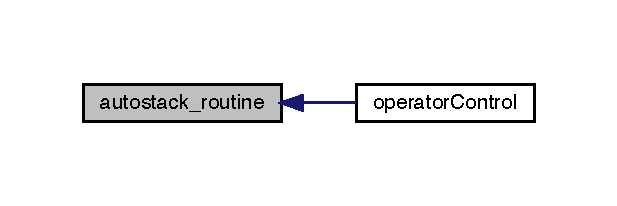
\includegraphics[width=296pt]{lifter_8h_a8a64fa88b389b39c236c5c57a7fb5c67_icgraph}
\end{center}
\end{figure}
\mbox{\label{lifter_8h_a2719740958fd8a5926f88f6194e820e3}} 
\index{lifter.\+h@{lifter.\+h}!get\+Lifter\+Height@{get\+Lifter\+Height}}
\index{get\+Lifter\+Height@{get\+Lifter\+Height}!lifter.\+h@{lifter.\+h}}
\paragraph{get\+Lifter\+Height()}
{\footnotesize\ttfamily double get\+Lifter\+Height (\begin{DoxyParamCaption}{ }\end{DoxyParamCaption})}



Gets the height of the lifter in inches. 

\begin{DoxyReturn}{Returns}
the height of the lifter. 
\end{DoxyReturn}
\begin{DoxyAuthor}{Author}
Chris Jerrett 
\end{DoxyAuthor}
\begin{DoxyDate}{Date}
9/17/2017 
\end{DoxyDate}


Definition at line \textbf{ 306} of file \textbf{ lifter.\+c}.



References \textbf{ get\+Lifter\+Ticks()}.


\begin{DoxyCode}
00306                          \{
00307   \textcolor{keywordtype}{unsigned} \textcolor{keywordtype}{int} ticks = getLifterTicks();
00308   \textcolor{keywordflow}{return} (-2 * pow(10, (-9 * ticks)) + 6 * (pow(10, (-6 * ticks * ticks))) +
00309           0.0198 * ticks + 2.3033);
00310 \}
\end{DoxyCode}
Here is the call graph for this function\+:
\nopagebreak
\begin{figure}[H]
\begin{center}
\leavevmode
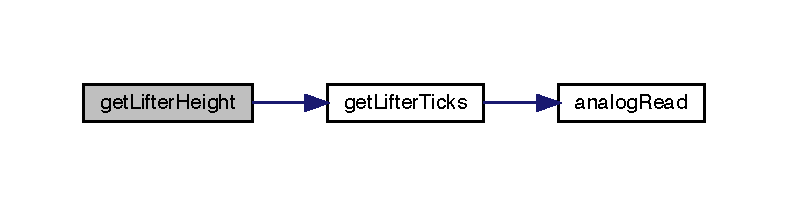
\includegraphics[width=350pt]{lifter_8h_a2719740958fd8a5926f88f6194e820e3_cgraph}
\end{center}
\end{figure}
\mbox{\label{lifter_8h_acdf909159b0406c48099843f2306be78}} 
\index{lifter.\+h@{lifter.\+h}!get\+Lifter\+Ticks@{get\+Lifter\+Ticks}}
\index{get\+Lifter\+Ticks@{get\+Lifter\+Ticks}!lifter.\+h@{lifter.\+h}}
\paragraph{get\+Lifter\+Ticks()}
{\footnotesize\ttfamily int get\+Lifter\+Ticks (\begin{DoxyParamCaption}{ }\end{DoxyParamCaption})}



Gets the value of the lifter pot. 

\begin{DoxyReturn}{Returns}
the value of the pot. 
\end{DoxyReturn}
\begin{DoxyAuthor}{Author}
Chris Jerrett 
\end{DoxyAuthor}
\begin{DoxyDate}{Date}
9/9/2017 
\end{DoxyDate}


Definition at line \textbf{ 297} of file \textbf{ lifter.\+c}.



References \textbf{ analog\+Read()}.



Referenced by \textbf{ get\+Lifter\+Height()}.


\begin{DoxyCode}
00297 \{ \textcolor{keywordflow}{return} analogRead(LIFTER); \}
\end{DoxyCode}
Here is the call graph for this function\+:
\nopagebreak
\begin{figure}[H]
\begin{center}
\leavevmode
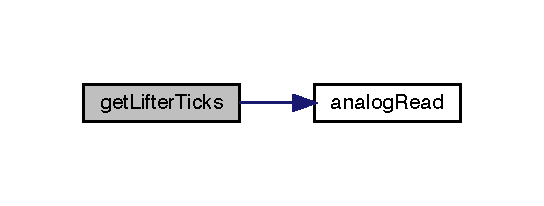
\includegraphics[width=261pt]{lifter_8h_acdf909159b0406c48099843f2306be78_cgraph}
\end{center}
\end{figure}
Here is the caller graph for this function\+:
\nopagebreak
\begin{figure}[H]
\begin{center}
\leavevmode
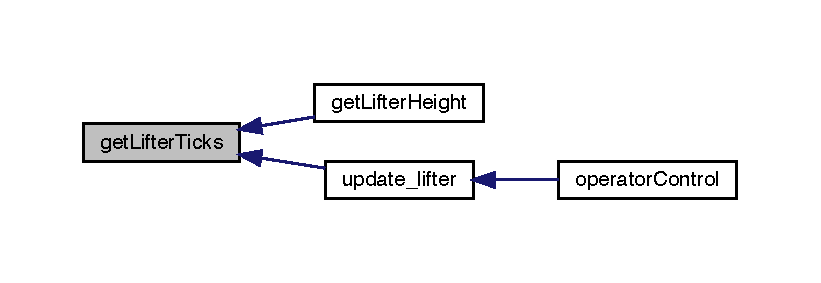
\includegraphics[width=272pt]{lifter_8h_acdf909159b0406c48099843f2306be78_icgraph}
\end{center}
\end{figure}
\mbox{\label{lifter_8h_a3738d33dc870f98243a93bddd855b43e}} 
\index{lifter.\+h@{lifter.\+h}!interrupt\+\_\+auto\+\_\+stack@{interrupt\+\_\+auto\+\_\+stack}}
\index{interrupt\+\_\+auto\+\_\+stack@{interrupt\+\_\+auto\+\_\+stack}!lifter.\+h@{lifter.\+h}}
\paragraph{interrupt\+\_\+auto\+\_\+stack()}
{\footnotesize\ttfamily void interrupt\+\_\+auto\+\_\+stack (\begin{DoxyParamCaption}\item[{void $\ast$}]{param }\end{DoxyParamCaption})}



Stpos an autostack in case of an error. 


\begin{DoxyParams}{Parameters}
{\em param} & ignore parameter \\
\hline
\end{DoxyParams}


Definition at line \textbf{ 8} of file \textbf{ lifter.\+c}.



References \textbf{ info()}, and \textbf{ lifter\+\_\+autostack\+\_\+routine\+\_\+interupt}.



Referenced by \textbf{ operator\+Control()}.


\begin{DoxyCode}
00008                                        \{
00009   info(\textcolor{stringliteral}{"int"});
00010   lifter_autostack_routine_interupt = \textcolor{keyword}{true};
00011 \}
\end{DoxyCode}
Here is the call graph for this function\+:
\nopagebreak
\begin{figure}[H]
\begin{center}
\leavevmode
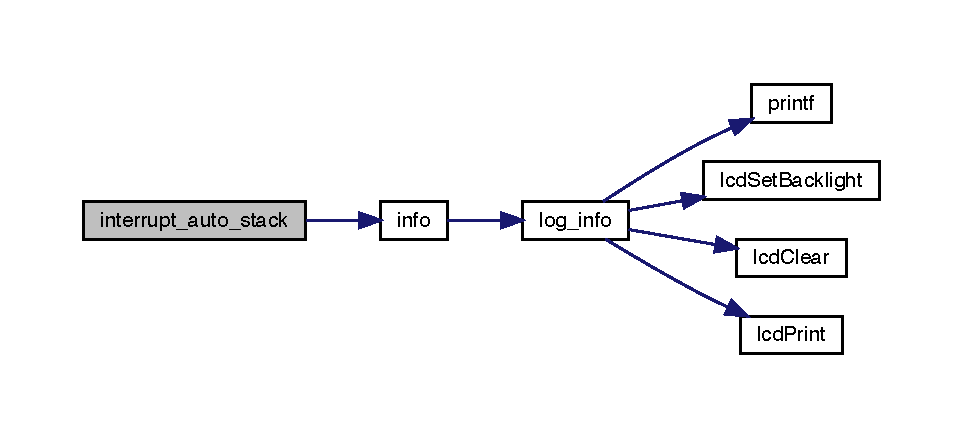
\includegraphics[width=350pt]{lifter_8h_a3738d33dc870f98243a93bddd855b43e_cgraph}
\end{center}
\end{figure}
Here is the caller graph for this function\+:
\nopagebreak
\begin{figure}[H]
\begin{center}
\leavevmode
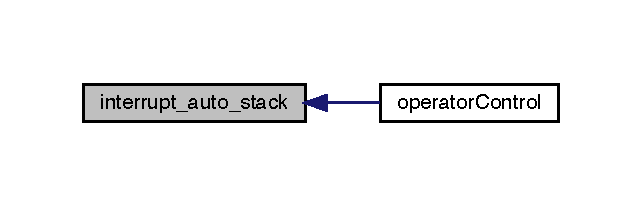
\includegraphics[width=308pt]{lifter_8h_a3738d33dc870f98243a93bddd855b43e_icgraph}
\end{center}
\end{figure}
\mbox{\label{lifter_8h_ab0460888f3213e5510bd25ae1e152a75}} 
\index{lifter.\+h@{lifter.\+h}!lifter\+Potentiometer\+To\+Degree@{lifter\+Potentiometer\+To\+Degree}}
\index{lifter\+Potentiometer\+To\+Degree@{lifter\+Potentiometer\+To\+Degree}!lifter.\+h@{lifter.\+h}}
\paragraph{lifter\+Potentiometer\+To\+Degree()}
{\footnotesize\ttfamily float lifter\+Potentiometer\+To\+Degree (\begin{DoxyParamCaption}\item[{int}]{x }\end{DoxyParamCaption})}



height of the lifter in degrees from 0 height 


\begin{DoxyParams}{Parameters}
{\em x} & the pot value \\
\hline
\end{DoxyParams}
\begin{DoxyReturn}{Returns}
the positions in degrees 
\end{DoxyReturn}
\begin{DoxyAuthor}{Author}
Chris Jerrett 
\end{DoxyAuthor}
\begin{DoxyDate}{Date}
10/13/2017 
\end{DoxyDate}


Definition at line \textbf{ 286} of file \textbf{ lifter.\+c}.


\begin{DoxyCode}
00286                                          \{
00287   \textcolor{keywordflow}{return} (x - INIT\_ROTATION) / TICK\_MAX * DEG\_MAX;
00288 \}
\end{DoxyCode}
\mbox{\label{lifter_8h_ad36c37086a91046af4e6f619618b7719}} 
\index{lifter.\+h@{lifter.\+h}!lower\+\_\+main\+\_\+lifter@{lower\+\_\+main\+\_\+lifter}}
\index{lower\+\_\+main\+\_\+lifter@{lower\+\_\+main\+\_\+lifter}!lifter.\+h@{lifter.\+h}}
\paragraph{lower\+\_\+main\+\_\+lifter()}
{\footnotesize\ttfamily void lower\+\_\+main\+\_\+lifter (\begin{DoxyParamCaption}{ }\end{DoxyParamCaption})}



Lowers the main lifter. 

\begin{DoxyAuthor}{Author}
Christian De\+Simone 
\end{DoxyAuthor}
\begin{DoxyDate}{Date}
9/12/2017 
\end{DoxyDate}


Definition at line \textbf{ 160} of file \textbf{ lifter.\+c}.



References \textbf{ set\+\_\+main\+\_\+lifter\+\_\+motors()}.


\begin{DoxyCode}
00160 \{ set_main_lifter_motors(MAX\_SPEED); \}
\end{DoxyCode}
Here is the call graph for this function\+:
\nopagebreak
\begin{figure}[H]
\begin{center}
\leavevmode
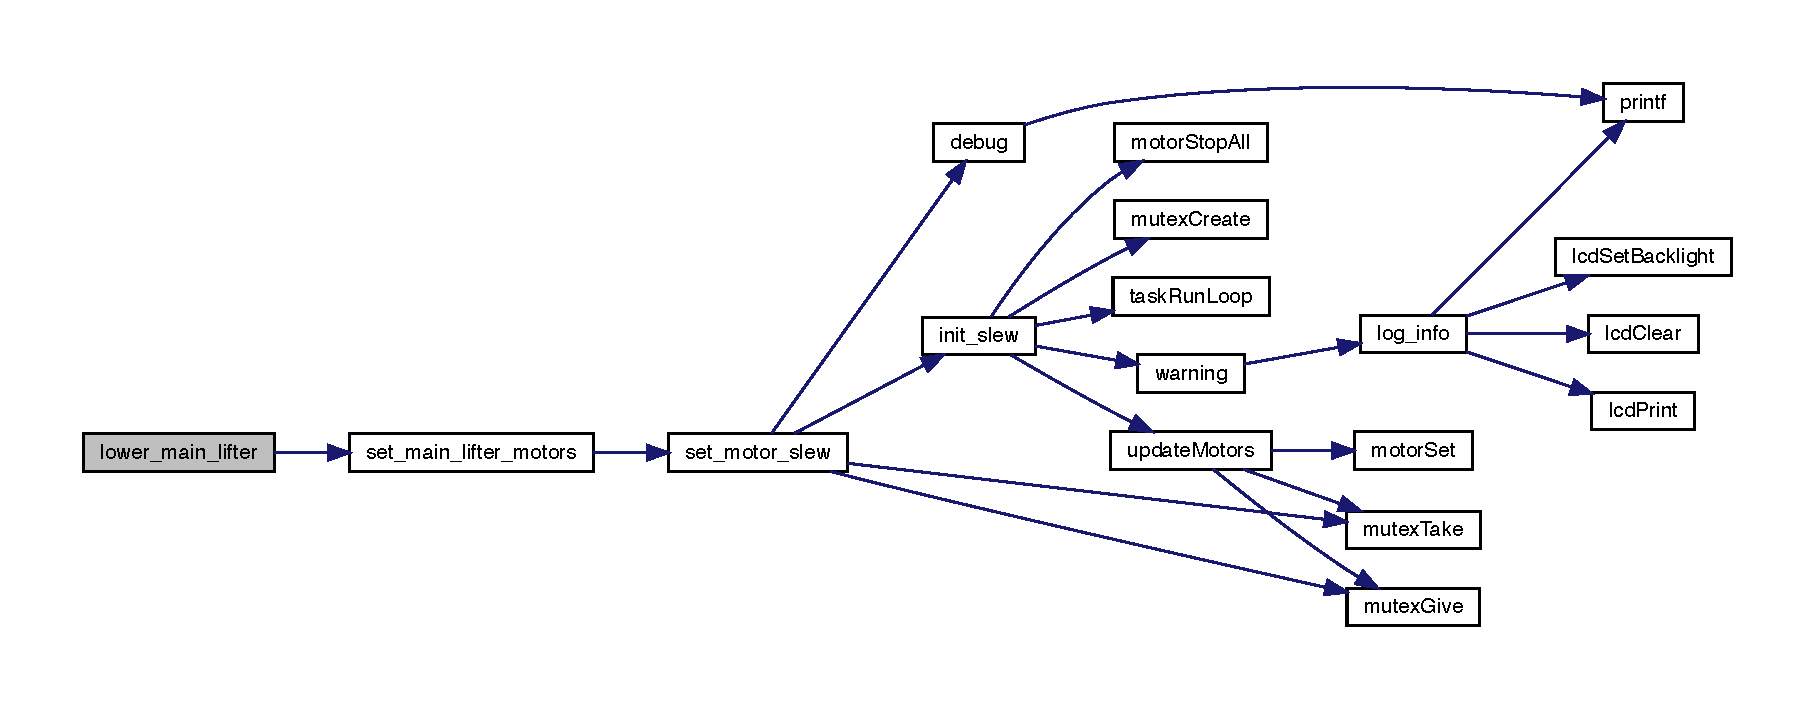
\includegraphics[width=350pt]{lifter_8h_ad36c37086a91046af4e6f619618b7719_cgraph}
\end{center}
\end{figure}
\mbox{\label{lifter_8h_af76abbd394bf206ab56fa237d776f2b3}} 
\index{lifter.\+h@{lifter.\+h}!lower\+\_\+secondary\+\_\+lifter@{lower\+\_\+secondary\+\_\+lifter}}
\index{lower\+\_\+secondary\+\_\+lifter@{lower\+\_\+secondary\+\_\+lifter}!lifter.\+h@{lifter.\+h}}
\paragraph{lower\+\_\+secondary\+\_\+lifter()}
{\footnotesize\ttfamily void lower\+\_\+secondary\+\_\+lifter (\begin{DoxyParamCaption}{ }\end{DoxyParamCaption})}



Lowers the secondary lifter. 

\begin{DoxyAuthor}{Author}
Christian De\+Simone 
\end{DoxyAuthor}
\begin{DoxyDate}{Date}
9/12/2017 
\end{DoxyDate}


Definition at line \textbf{ 176} of file \textbf{ lifter.\+c}.



References \textbf{ set\+\_\+secondary\+\_\+lifter\+\_\+motors()}.


\begin{DoxyCode}
00176 \{ set_secondary_lifter_motors(MAX\_SPEED); \}
\end{DoxyCode}
Here is the call graph for this function\+:
\nopagebreak
\begin{figure}[H]
\begin{center}
\leavevmode
\includegraphics[width=350pt]{lifter_8h_af76abbd394bf206ab56fa237d776f2b3_cgraph}
\end{center}
\end{figure}
\mbox{\label{lifter_8h_a2e2bd38b5b8b52378f3510368bf8aa0a}} 
\index{lifter.\+h@{lifter.\+h}!raise\+\_\+main\+\_\+lifter@{raise\+\_\+main\+\_\+lifter}}
\index{raise\+\_\+main\+\_\+lifter@{raise\+\_\+main\+\_\+lifter}!lifter.\+h@{lifter.\+h}}
\paragraph{raise\+\_\+main\+\_\+lifter()}
{\footnotesize\ttfamily void raise\+\_\+main\+\_\+lifter (\begin{DoxyParamCaption}{ }\end{DoxyParamCaption})}



Raises the main lifter. 

\begin{DoxyAuthor}{Author}
Christian De\+Simone 
\end{DoxyAuthor}
\begin{DoxyDate}{Date}
9/12/2017 
\end{DoxyDate}


Definition at line \textbf{ 152} of file \textbf{ lifter.\+c}.



References \textbf{ set\+\_\+main\+\_\+lifter\+\_\+motors()}.


\begin{DoxyCode}
00152 \{ set_main_lifter_motors(MAX\_SPEED); \}
\end{DoxyCode}
Here is the call graph for this function\+:
\nopagebreak
\begin{figure}[H]
\begin{center}
\leavevmode
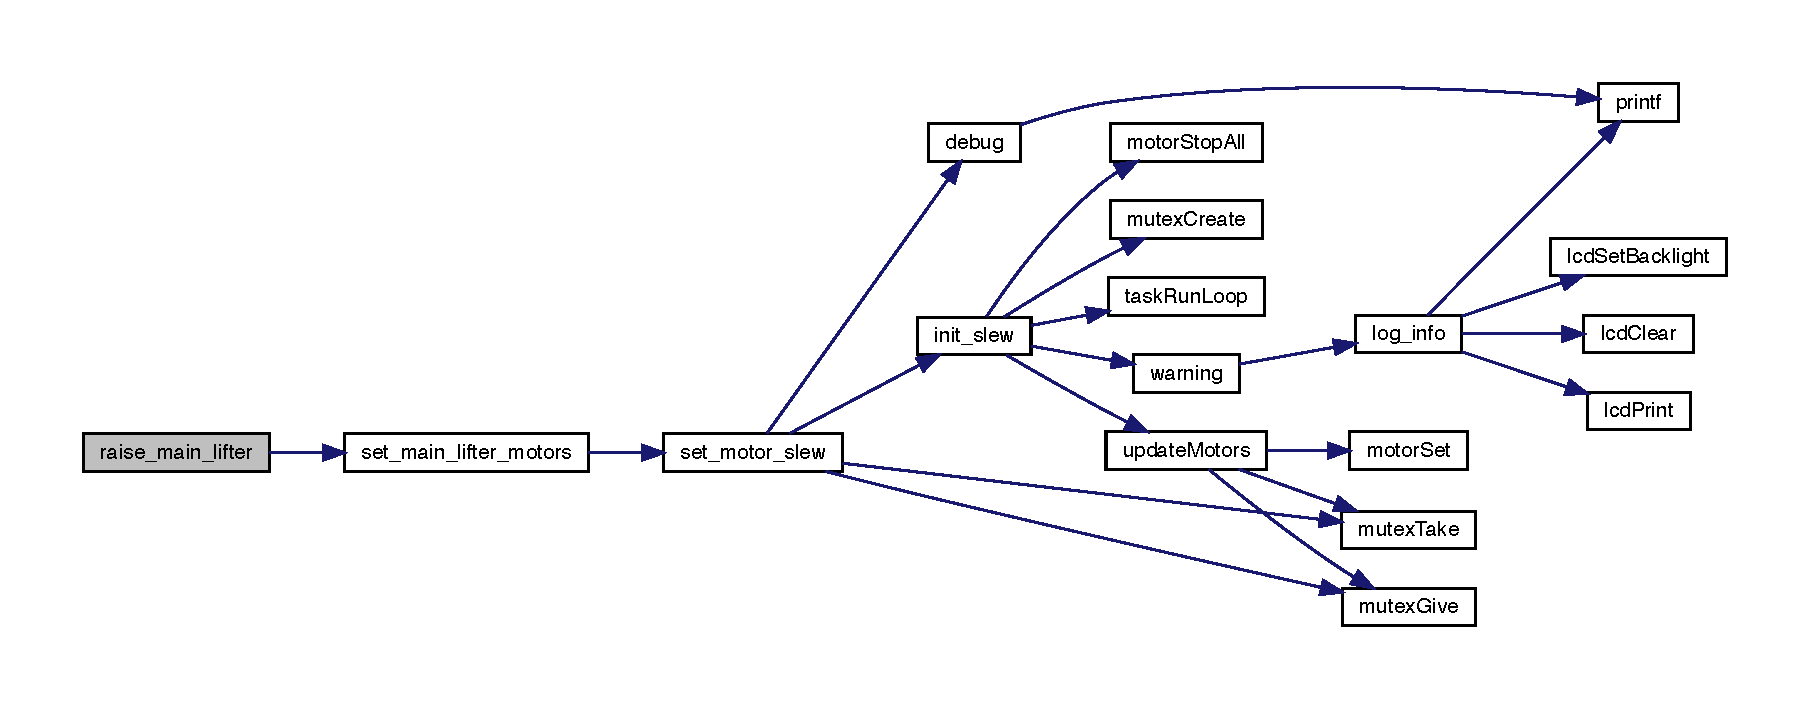
\includegraphics[width=350pt]{lifter_8h_a2e2bd38b5b8b52378f3510368bf8aa0a_cgraph}
\end{center}
\end{figure}
\mbox{\label{lifter_8h_a786f679ea48bb8c80e00fbac9a69911b}} 
\index{lifter.\+h@{lifter.\+h}!raise\+\_\+secondary\+\_\+lifter@{raise\+\_\+secondary\+\_\+lifter}}
\index{raise\+\_\+secondary\+\_\+lifter@{raise\+\_\+secondary\+\_\+lifter}!lifter.\+h@{lifter.\+h}}
\paragraph{raise\+\_\+secondary\+\_\+lifter()}
{\footnotesize\ttfamily void raise\+\_\+secondary\+\_\+lifter (\begin{DoxyParamCaption}{ }\end{DoxyParamCaption})}



Raises the main lifter. 

\begin{DoxyAuthor}{Author}
Christian De\+Simone 
\end{DoxyAuthor}
\begin{DoxyDate}{Date}
9/12/2017 
\end{DoxyDate}


Definition at line \textbf{ 168} of file \textbf{ lifter.\+c}.



References \textbf{ set\+\_\+secondary\+\_\+lifter\+\_\+motors()}.



Referenced by \textbf{ autostack\+\_\+routine()}.


\begin{DoxyCode}
00168 \{ set_secondary_lifter_motors(MIN\_SPEED / 1.5); \}
\end{DoxyCode}
Here is the call graph for this function\+:
\nopagebreak
\begin{figure}[H]
\begin{center}
\leavevmode
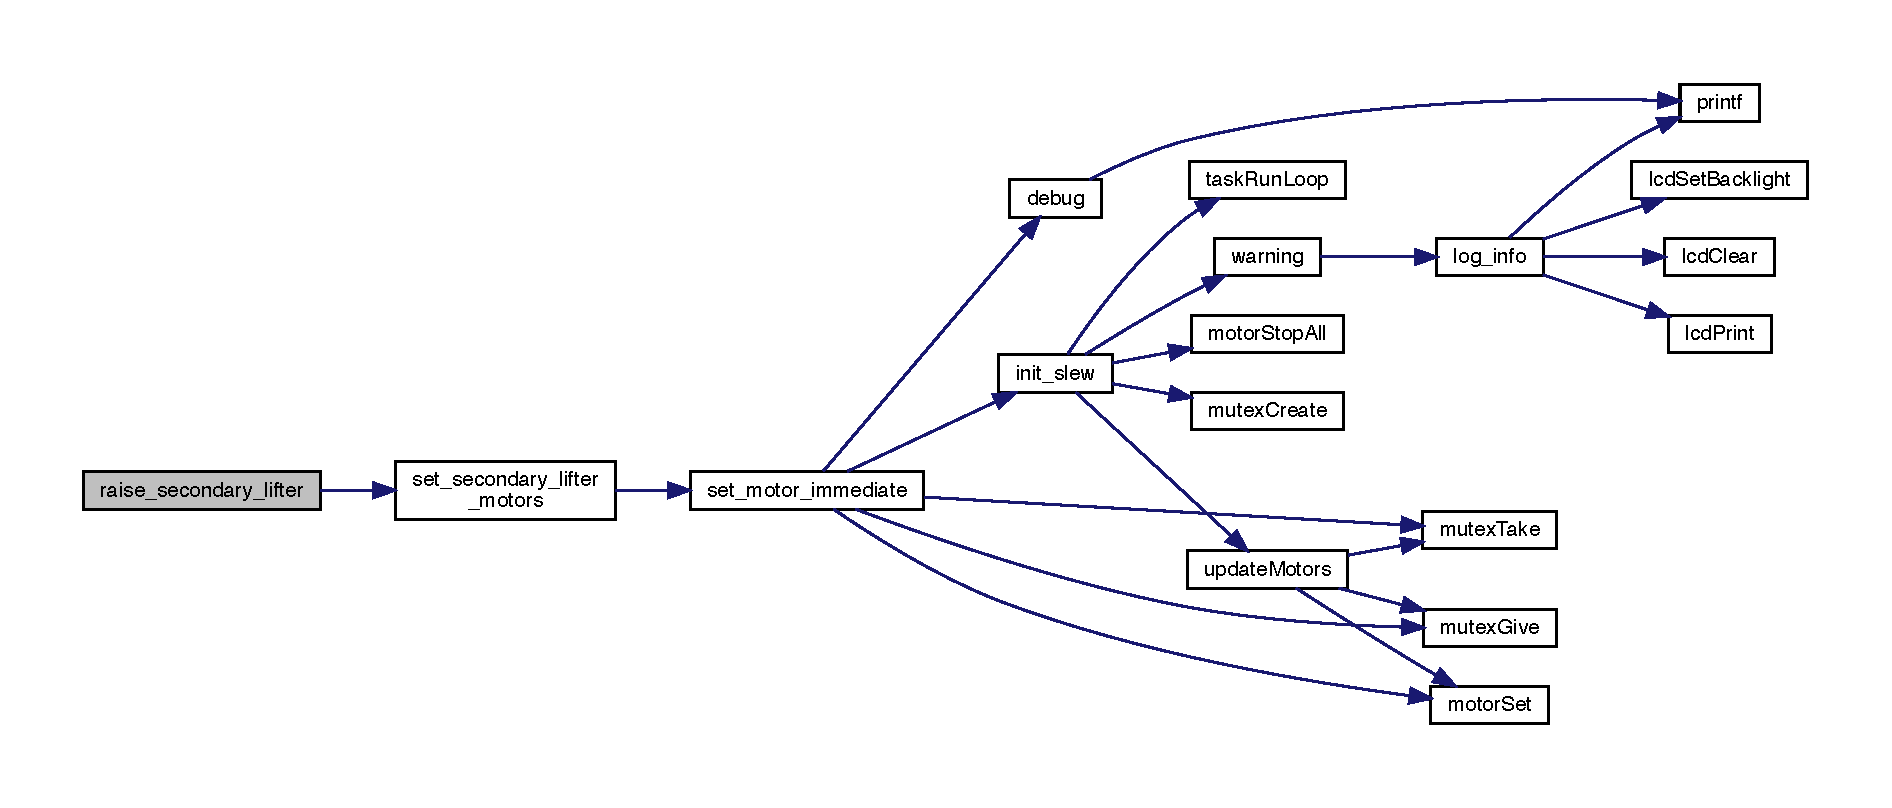
\includegraphics[width=350pt]{lifter_8h_a786f679ea48bb8c80e00fbac9a69911b_cgraph}
\end{center}
\end{figure}
Here is the caller graph for this function\+:
\nopagebreak
\begin{figure}[H]
\begin{center}
\leavevmode
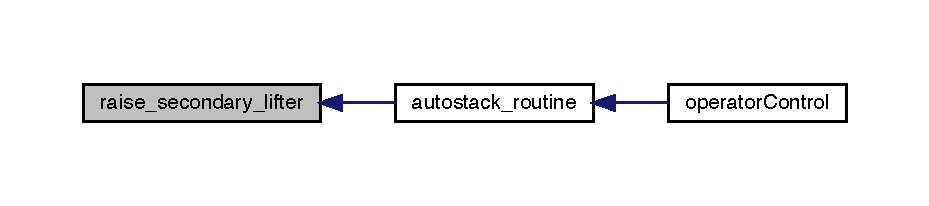
\includegraphics[width=350pt]{lifter_8h_a786f679ea48bb8c80e00fbac9a69911b_icgraph}
\end{center}
\end{figure}
\mbox{\label{lifter_8h_abddc7cb502e12fa277b627c90a45efb1}} 
\index{lifter.\+h@{lifter.\+h}!set\+\_\+lifter\+\_\+pos@{set\+\_\+lifter\+\_\+pos}}
\index{set\+\_\+lifter\+\_\+pos@{set\+\_\+lifter\+\_\+pos}!lifter.\+h@{lifter.\+h}}
\paragraph{set\+\_\+lifter\+\_\+pos()}
{\footnotesize\ttfamily void set\+\_\+lifter\+\_\+pos (\begin{DoxyParamCaption}\item[{int}]{pos }\end{DoxyParamCaption})}



Sets the lifter positions to the given value. 


\begin{DoxyParams}{Parameters}
{\em pos} & The height in inches \\
\hline
\end{DoxyParams}
\begin{DoxyAuthor}{Author}
Chris Jerrett 
\end{DoxyAuthor}
\begin{DoxyDate}{Date}
9/12/2017 
\end{DoxyDate}


Definition at line \textbf{ 144} of file \textbf{ lifter.\+c}.


\begin{DoxyCode}
00144 \{\}
\end{DoxyCode}
\mbox{\label{lifter_8h_ad00a195af30f246924d6e1a30095b882}} 
\index{lifter.\+h@{lifter.\+h}!set\+\_\+main\+\_\+lifter\+\_\+motors@{set\+\_\+main\+\_\+lifter\+\_\+motors}}
\index{set\+\_\+main\+\_\+lifter\+\_\+motors@{set\+\_\+main\+\_\+lifter\+\_\+motors}!lifter.\+h@{lifter.\+h}}
\paragraph{set\+\_\+main\+\_\+lifter\+\_\+motors()}
{\footnotesize\ttfamily void set\+\_\+main\+\_\+lifter\+\_\+motors (\begin{DoxyParamCaption}\item[{const int}]{v }\end{DoxyParamCaption})}



Sets the main lifter motors to the given value. 


\begin{DoxyParams}{Parameters}
{\em v} & value for the lifter motor. Between -\/128 -\/ 127, any values outside are clamped. \\
\hline
\end{DoxyParams}
\begin{DoxyAuthor}{Author}
Chris Jerrett 
\end{DoxyAuthor}
\begin{DoxyDate}{Date}
9/9/2017 
\end{DoxyDate}


Definition at line \textbf{ 133} of file \textbf{ lifter.\+c}.



References \textbf{ set\+\_\+motor\+\_\+slew()}.



Referenced by \textbf{ auton\+\_\+rasie\+\_\+main\+\_\+lifter()}, \textbf{ autostack\+\_\+routine()}, \textbf{ lower\+\_\+main\+\_\+lifter()}, \textbf{ main\+\_\+lifter\+\_\+update()}, \textbf{ quit\+\_\+auto\+\_\+static()}, and \textbf{ raise\+\_\+main\+\_\+lifter()}.


\begin{DoxyCode}
00133                                          \{
00134   set_motor_slew(MOTOR\_MAIN\_LIFTER, v);
00135 \}
\end{DoxyCode}
Here is the call graph for this function\+:
\nopagebreak
\begin{figure}[H]
\begin{center}
\leavevmode
\includegraphics[width=350pt]{lifter_8h_ad00a195af30f246924d6e1a30095b882_cgraph}
\end{center}
\end{figure}
Here is the caller graph for this function\+:
\nopagebreak
\begin{figure}[H]
\begin{center}
\leavevmode
\includegraphics[width=350pt]{lifter_8h_ad00a195af30f246924d6e1a30095b882_icgraph}
\end{center}
\end{figure}
\mbox{\label{lifter_8h_a78640d547d9361951a92d0bc00939536}} 
\index{lifter.\+h@{lifter.\+h}!set\+\_\+secondary\+\_\+lifter\+\_\+motors@{set\+\_\+secondary\+\_\+lifter\+\_\+motors}}
\index{set\+\_\+secondary\+\_\+lifter\+\_\+motors@{set\+\_\+secondary\+\_\+lifter\+\_\+motors}!lifter.\+h@{lifter.\+h}}
\paragraph{set\+\_\+secondary\+\_\+lifter\+\_\+motors()}
{\footnotesize\ttfamily void set\+\_\+secondary\+\_\+lifter\+\_\+motors (\begin{DoxyParamCaption}\item[{const int}]{v }\end{DoxyParamCaption})}



Sets the secondary lifter motors to the given value. 


\begin{DoxyParams}{Parameters}
{\em v} & value for the lifter motor. Between -\/128 -\/ 127, any values outside are clamped. \\
\hline
\end{DoxyParams}
\begin{DoxyAuthor}{Author}
Chris Jerrett 
\end{DoxyAuthor}
\begin{DoxyDate}{Date}
1/6/2018 
\end{DoxyDate}


Definition at line \textbf{ 121} of file \textbf{ lifter.\+c}.



References \textbf{ set\+\_\+motor\+\_\+immediate()}.



Referenced by \textbf{ auton\+\_\+raise\+\_\+sec\+\_\+lifter\+\_\+max()}, \textbf{ autonomous()}, \textbf{ autostack\+\_\+routine()}, \textbf{ deploy\+\_\+seoncdary\+\_\+lifter()}, \textbf{ lower\+\_\+secondary\+\_\+lifter()}, \textbf{ quit\+\_\+auto\+\_\+static()}, \textbf{ raise\+\_\+secondary\+\_\+lifter()}, and \textbf{ secondary\+\_\+lifter\+\_\+update()}.


\begin{DoxyCode}
00121                                               \{
00122   set_motor_immediate(MOTOR\_SECONDARY\_LIFTER, v);
00123 \}
\end{DoxyCode}
Here is the call graph for this function\+:
\nopagebreak
\begin{figure}[H]
\begin{center}
\leavevmode
\includegraphics[width=350pt]{lifter_8h_a78640d547d9361951a92d0bc00939536_cgraph}
\end{center}
\end{figure}
Here is the caller graph for this function\+:
\nopagebreak
\begin{figure}[H]
\begin{center}
\leavevmode
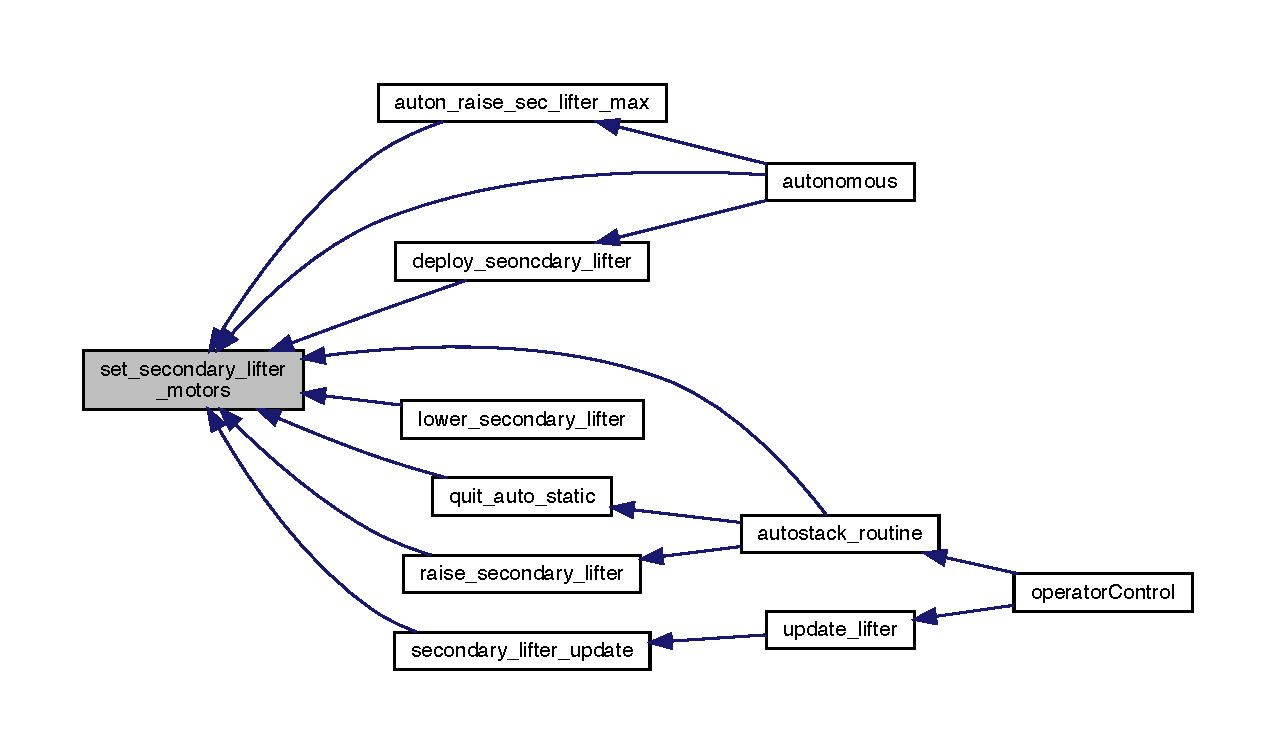
\includegraphics[width=350pt]{lifter_8h_a78640d547d9361951a92d0bc00939536_icgraph}
\end{center}
\end{figure}
\mbox{\label{lifter_8h_a59bb7413777ca16aba124aaedf95c79b}} 
\index{lifter.\+h@{lifter.\+h}!update\+\_\+lifter@{update\+\_\+lifter}}
\index{update\+\_\+lifter@{update\+\_\+lifter}!lifter.\+h@{lifter.\+h}}
\paragraph{update\+\_\+lifter()}
{\footnotesize\ttfamily void update\+\_\+lifter (\begin{DoxyParamCaption}{ }\end{DoxyParamCaption})}



Updates the lifter in teleop. 

\begin{DoxyAuthor}{Author}
Chris Jerrett 
\end{DoxyAuthor}
\begin{DoxyDate}{Date}
9/9/2017 
\end{DoxyDate}


Definition at line \textbf{ 272} of file \textbf{ lifter.\+c}.



References \textbf{ analog\+Read()}, \textbf{ main\+\_\+lifter\+\_\+update()}, \textbf{ printf()}, \textbf{ secondary\+\_\+lifter\+\_\+update()}, and \textbf{ secondary\+\_\+override}.



Referenced by \textbf{ operator\+Control()}.


\begin{DoxyCode}
00272                      \{
00273   printf(\textcolor{stringliteral}{"%d \(\backslash\)n"}, analogRead(SECONDARY\_LIFTER\_POT\_PORT));
00274   main_lifter_update();
00275   \textcolor{keywordflow}{if} (!secondary_override)
00276     secondary_lifter_update();
00277 \}
\end{DoxyCode}
Here is the call graph for this function\+:
\nopagebreak
\begin{figure}[H]
\begin{center}
\leavevmode
\includegraphics[width=350pt]{lifter_8h_a59bb7413777ca16aba124aaedf95c79b_cgraph}
\end{center}
\end{figure}
Here is the caller graph for this function\+:
\nopagebreak
\begin{figure}[H]
\begin{center}
\leavevmode
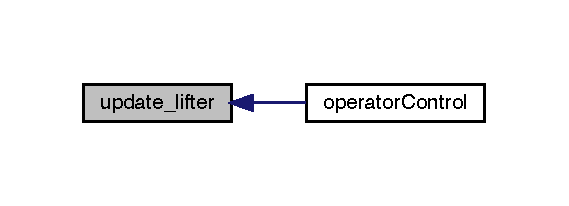
\includegraphics[width=273pt]{lifter_8h_a59bb7413777ca16aba124aaedf95c79b_icgraph}
\end{center}
\end{figure}

\subsection{lifter.\+h}
\label{lifter_8h_source}\index{include/lifter.\+h@{include/lifter.\+h}}

\begin{DoxyCode}
00001 
00007 \textcolor{preprocessor}{#ifndef \_LIFTER\_H\_}
00008 \textcolor{preprocessor}{#define \_LIFTER\_H\_}
00009 
00010 \textcolor{preprocessor}{#include "controller.h"}
00011 \textcolor{preprocessor}{#include "drive.h"}
00012 \textcolor{preprocessor}{#include "motor_ports.h"}
00013 \textcolor{preprocessor}{#include "potentiometer.h"}
00014 \textcolor{preprocessor}{#include "sensors.h"}
00015 \textcolor{preprocessor}{#include "slew.h"}
00016 \textcolor{preprocessor}{#include <API.h>}
00017 
00021 \textcolor{preprocessor}{#define INIT\_ROTATION 680}
00022 
00026 \textcolor{preprocessor}{#define SECONDARY\_LIFTER\_P .05}
00027 
00031 \textcolor{preprocessor}{#define SECONDARY\_LIFTER\_D 0}
00032 
00036 \textcolor{preprocessor}{#define SECONDARY\_LIFTER\_I 0.000}
00037 
00041 \textcolor{preprocessor}{#define MAIN\_LIFTER\_P 0}
00042 
00046 \textcolor{preprocessor}{#define MAIN\_LIFTER\_D 0}
00047 
00051 \textcolor{preprocessor}{#define MAIN\_LIFTER\_I 0.0000001}
00052 
00056 \textcolor{preprocessor}{#define THRESHOLD 10}
00057 
00061 \textcolor{preprocessor}{#define HEIGHT 19.1 - 3.8}
00062 
00066 \textcolor{preprocessor}{#define LIFTER\_UP PARTNER, 6, JOY\_UP}
00067 
00071 \textcolor{preprocessor}{#define LIFTER\_DOWN PARTNER, 6, JOY\_DOWN}
00072 
00076 \textcolor{preprocessor}{#define SECONDARY\_LIFTER\_UP PARTNER, 5, JOY\_UP}
00077 
00081 \textcolor{preprocessor}{#define SECONDARY\_LIFTER\_DOWN PARTNER, 5, JOY\_DOWN}
00082 
00086 \textcolor{preprocessor}{#define LIFTER\_DRIVER\_LOAD MASTER, RIGHT\_BUTTONS, JOY\_RIGHT}
00087 
00091 \textcolor{preprocessor}{#define LIFTER\_UP\_PARTNER PARTNER, 5, JOY\_UP}
00092 
00096 \textcolor{preprocessor}{#define LIFTER\_DOWN\_PARTNER PARTNER, 5, JOY\_DOWN}
00097 
00101 \textcolor{preprocessor}{#define SECONDARY\_LIFTER\_POT\_PORT 2}
00102 
00106 \textcolor{preprocessor}{#define SECONDARY\_LIFTER\_MAX\_HEIGHT 3120}
00107 
00111 \textcolor{preprocessor}{#define SECONDARY\_LIFTER\_MIN\_HEIGHT 2000}
00112 
00116 \textcolor{preprocessor}{#define MAIN\_LIFTER\_POT 1}
00117 
00121 \textcolor{preprocessor}{#define MAIN\_LIFTER\_MIN\_HEIGHT 1700}
00122 
00131 \textcolor{keywordtype}{void} set_secondary_lifter_motors(\textcolor{keyword}{const} \textcolor{keywordtype}{int} v);
00132 
00141 \textcolor{keywordtype}{void} set_main_lifter_motors(\textcolor{keyword}{const} \textcolor{keywordtype}{int} v);
00142 
00150 \textcolor{keywordtype}{void} set_lifter_pos(\textcolor{keywordtype}{int} pos);
00151 
00158 \textcolor{keywordtype}{void} raise_main_lifter();
00159 
00166 \textcolor{keywordtype}{void} lower_main_lifter();
00167 
00174 \textcolor{keywordtype}{void} raise_secondary_lifter();
00175 
00182 \textcolor{keywordtype}{void} lower_secondary_lifter();
00183 
00190 \textcolor{keywordtype}{void} update_lifter();
00191 
00200 \textcolor{keywordtype}{float} lifterPotentiometerToDegree(\textcolor{keywordtype}{int} x);
00201 
00209 \textcolor{keywordtype}{int} getLifterTicks();
00210 
00218 \textcolor{keywordtype}{double} getLifterHeight();
00219 
00224 \textcolor{keywordtype}{void} autostack_routine(\textcolor{keywordtype}{void} *param);
00225 
00230 \textcolor{keywordtype}{void} interrupt_auto_stack(\textcolor{keywordtype}{void} *param);
00231 
00232 \textcolor{preprocessor}{#endif}
\end{DoxyCode}

\subsection{include/localization.h File Reference}
\label{localization_8h}\index{include/localization.\+h@{include/localization.\+h}}


Declarations and macros for determining the location of the robot. [W\+IP].  


{\ttfamily \#include \char`\"{}encoders.\+h\char`\"{}}\newline
{\ttfamily \#include \char`\"{}matrix.\+h\char`\"{}}\newline
{\ttfamily \#include $<$A\+P\+I.\+h$>$}\newline
{\ttfamily \#include $<$math.\+h$>$}\newline
\subsubsection*{Data Structures}
\begin{DoxyCompactItemize}
\item 
struct \textbf{ location}
\end{DoxyCompactItemize}
\subsubsection*{Macros}
\begin{DoxyCompactItemize}
\item 
\#define \textbf{ L\+O\+C\+A\+L\+I\+Z\+A\+T\+I\+O\+N\+\_\+\+U\+P\+D\+A\+T\+E\+\_\+\+F\+R\+E\+Q\+U\+E\+N\+CY}~0.\+500
\end{DoxyCompactItemize}
\subsubsection*{Functions}
\begin{DoxyCompactItemize}
\item 
int \textbf{ calculate\+\_\+encoder\+\_\+angle} ()
\item 
struct \textbf{ location} \textbf{ get\+\_\+position} ()
\begin{DoxyCompactList}\small\item\em Gets the current posituion of the robot. \end{DoxyCompactList}\item 
bool \textbf{ init\+\_\+localization} (const unsigned char gyro1, unsigned short multiplier, int start\+\_\+x, int start\+\_\+y, int start\+\_\+theta)
\begin{DoxyCompactList}\small\item\em Starts the localization process. \end{DoxyCompactList}\item 
void \textbf{ update\+\_\+position} ()
\begin{DoxyCompactList}\small\item\em Updates the position from the localization. \end{DoxyCompactList}\end{DoxyCompactItemize}


\subsubsection{Detailed Description}
Declarations and macros for determining the location of the robot. [W\+IP]. 

\begin{DoxyAuthor}{Author}
Chris Jerrett, Christian Desimone 
\end{DoxyAuthor}
\begin{DoxyDate}{Date}
9/27/2017 
\end{DoxyDate}


Definition in file \textbf{ localization.\+h}.



\subsubsection{Macro Definition Documentation}
\mbox{\label{localization_8h_a4fa0a97f6aafe983a46ffc7188d1fab5}} 
\index{localization.\+h@{localization.\+h}!L\+O\+C\+A\+L\+I\+Z\+A\+T\+I\+O\+N\+\_\+\+U\+P\+D\+A\+T\+E\+\_\+\+F\+R\+E\+Q\+U\+E\+N\+CY@{L\+O\+C\+A\+L\+I\+Z\+A\+T\+I\+O\+N\+\_\+\+U\+P\+D\+A\+T\+E\+\_\+\+F\+R\+E\+Q\+U\+E\+N\+CY}}
\index{L\+O\+C\+A\+L\+I\+Z\+A\+T\+I\+O\+N\+\_\+\+U\+P\+D\+A\+T\+E\+\_\+\+F\+R\+E\+Q\+U\+E\+N\+CY@{L\+O\+C\+A\+L\+I\+Z\+A\+T\+I\+O\+N\+\_\+\+U\+P\+D\+A\+T\+E\+\_\+\+F\+R\+E\+Q\+U\+E\+N\+CY}!localization.\+h@{localization.\+h}}
\paragraph{L\+O\+C\+A\+L\+I\+Z\+A\+T\+I\+O\+N\+\_\+\+U\+P\+D\+A\+T\+E\+\_\+\+F\+R\+E\+Q\+U\+E\+N\+CY}
{\footnotesize\ttfamily \#define L\+O\+C\+A\+L\+I\+Z\+A\+T\+I\+O\+N\+\_\+\+U\+P\+D\+A\+T\+E\+\_\+\+F\+R\+E\+Q\+U\+E\+N\+CY~0.\+500}

How often the localization code updates the position. 

Definition at line \textbf{ 19} of file \textbf{ localization.\+h}.



Referenced by \textbf{ calculate\+\_\+gryo\+\_\+anglular\+\_\+velocity()}, \textbf{ init\+\_\+localization()}, and \textbf{ integrate\+\_\+gyro\+\_\+w()}.



\subsubsection{Function Documentation}
\mbox{\label{localization_8h_a5dd17937f5561711cd12cdefa8d31869}} 
\index{localization.\+h@{localization.\+h}!calculate\+\_\+encoder\+\_\+angle@{calculate\+\_\+encoder\+\_\+angle}}
\index{calculate\+\_\+encoder\+\_\+angle@{calculate\+\_\+encoder\+\_\+angle}!localization.\+h@{localization.\+h}}
\paragraph{calculate\+\_\+encoder\+\_\+angle()}
{\footnotesize\ttfamily int calculate\+\_\+encoder\+\_\+angle (\begin{DoxyParamCaption}{ }\end{DoxyParamCaption})}



Definition at line \textbf{ 101} of file \textbf{ localization.\+c}.



References \textbf{ C\+PR}, \textbf{ get\+\_\+encoder\+\_\+ticks()}, and \textbf{ W\+I\+D\+TH}.



Referenced by \textbf{ autonomous()}.

\mbox{\label{localization_8h_aadbff35bb757f60bc348d4d778f57a2f}} 
\index{localization.\+h@{localization.\+h}!get\+\_\+position@{get\+\_\+position}}
\index{get\+\_\+position@{get\+\_\+position}!localization.\+h@{localization.\+h}}
\paragraph{get\+\_\+position()}
{\footnotesize\ttfamily struct \textbf{ location} get\+\_\+position (\begin{DoxyParamCaption}{ }\end{DoxyParamCaption})}



Gets the current posituion of the robot. 


\begin{DoxyParams}{Parameters}
{\em gyro1} & The first gyro \\
\hline
\end{DoxyParams}
\begin{DoxyReturn}{Returns}
the loacation of the robot as a struct. 
\end{DoxyReturn}


Definition at line \textbf{ 32} of file \textbf{ localization.\+c}.

\mbox{\label{localization_8h_afdd0147de6aa15957e9a125f9cd20578}} 
\index{localization.\+h@{localization.\+h}!init\+\_\+localization@{init\+\_\+localization}}
\index{init\+\_\+localization@{init\+\_\+localization}!localization.\+h@{localization.\+h}}
\paragraph{init\+\_\+localization()}
{\footnotesize\ttfamily bool init\+\_\+localization (\begin{DoxyParamCaption}\item[{const unsigned char}]{gyro1,  }\item[{unsigned short}]{multiplier,  }\item[{int}]{start\+\_\+x,  }\item[{int}]{start\+\_\+y,  }\item[{int}]{start\+\_\+theta }\end{DoxyParamCaption})}



Starts the localization process. 

\begin{DoxyAuthor}{Author}
Chris Jerrett
\end{DoxyAuthor}

\begin{DoxyParams}{Parameters}
{\em gyro1} & The first gyro  The multiplier parameter can tune the gyro to adapt to specific sensors. The default value at this time is 196; higher values will increase the number of degrees reported for a fixed actual rotation, while lower values will decrease the number of degrees reported. If your robot is consistently turning too far, increase the multiplier, and if it is not turning far enough, decrease the multiplier. \\
\hline
\end{DoxyParams}


Definition at line \textbf{ 123} of file \textbf{ localization.\+c}.



References \textbf{ g1}, \textbf{ last\+\_\+call}, \textbf{ localization\+\_\+task}, \textbf{ L\+O\+C\+A\+L\+I\+Z\+A\+T\+I\+O\+N\+\_\+\+U\+P\+D\+A\+T\+E\+\_\+\+F\+R\+E\+Q\+U\+E\+N\+CY}, \textbf{ make\+Matrix()}, and \textbf{ update\+\_\+position()}.

\mbox{\label{localization_8h_afacd5e0b3d5e677df26a4402bbd9ec9e}} 
\index{localization.\+h@{localization.\+h}!update\+\_\+position@{update\+\_\+position}}
\index{update\+\_\+position@{update\+\_\+position}!localization.\+h@{localization.\+h}}
\paragraph{update\+\_\+position()}
{\footnotesize\ttfamily void update\+\_\+position (\begin{DoxyParamCaption}{ }\end{DoxyParamCaption})}



Updates the position from the localization. 

\begin{DoxyAuthor}{Author}
Chris Jerrett 
\end{DoxyAuthor}


Definition at line \textbf{ 39} of file \textbf{ localization.\+c}.



References \textbf{ calculate\+\_\+accelerometer\+\_\+odemetry()}, and \textbf{ last\+\_\+call}.



Referenced by \textbf{ init\+\_\+localization()}.


\section{localization.\+h}
\label{localization_8h_source}\index{include/localization.\+h@{include/localization.\+h}}

\begin{DoxyCode}
00001 
00007 \textcolor{preprocessor}{#ifndef \_LOCALIZATION\_H\_}
00008 \textcolor{preprocessor}{#define \_LOCALIZATION\_H\_}
00009 
00010 \textcolor{preprocessor}{#include <API.h>}
00011 \textcolor{preprocessor}{#include "encoders.h"}
00012 \textcolor{preprocessor}{#include <math.h>}
00013 \textcolor{preprocessor}{#include "matrix.h"}
00014 
00018 \textcolor{preprocessor}{#define LOCALIZATION\_UPDATE\_FREQUENCY 0.500}
00019 
00023 \textcolor{keyword}{struct }location \{
00024   \textcolor{keywordtype}{int} x;
00025   \textcolor{keywordtype}{int} y;
00026   \textcolor{keywordtype}{int} theta;
00027 \};
00028 
00040 \textcolor{keywordtype}{bool} init_localization(\textcolor{keyword}{const} \textcolor{keywordtype}{unsigned} \textcolor{keywordtype}{char} gyro1, \textcolor{keywordtype}{unsigned} \textcolor{keywordtype}{short} multiplier, \textcolor{keywordtype}{int} start\_x, \textcolor{keywordtype}{int} start\_y, \textcolor{keywordtype}{int} 
      start\_theta);
00041 
00048 \textcolor{keyword}{struct }location get_position();
00049 
00055 \textcolor{keywordtype}{void} update_position();
00056 
00057 \textcolor{preprocessor}{#endif}
\end{DoxyCode}

\subsection{include/log.h File Reference}
\label{log_8h}\index{include/log.\+h@{include/log.\+h}}


Contains logging functions.  


{\ttfamily \#include \char`\"{}lcd.\+h\char`\"{}}\newline
{\ttfamily \#include $<$A\+P\+I.\+h$>$}\newline
\subsubsection*{Macros}
\begin{DoxyCompactItemize}
\item 
\#define \textbf{ D\+E\+B\+UG}~4
\begin{DoxyCompactList}\small\item\em logging only info debug. most verbose level \end{DoxyCompactList}\item 
\#define \textbf{ E\+R\+R\+OR}~1
\begin{DoxyCompactList}\small\item\em logging only errors. Also displays error to lcd \end{DoxyCompactList}\item 
\#define \textbf{ I\+N\+FO}~3
\begin{DoxyCompactList}\small\item\em logging only info messages and higher. \end{DoxyCompactList}\item 
\#define \textbf{ N\+O\+NE}~0
\begin{DoxyCompactList}\small\item\em No logging. Should be used in competition to reduce serial communication. \end{DoxyCompactList}\item 
\#define \textbf{ W\+A\+R\+N\+I\+NG}~2
\begin{DoxyCompactList}\small\item\em logs errors and warnings. Also displays error to lcd \end{DoxyCompactList}\end{DoxyCompactItemize}
\subsubsection*{Functions}
\begin{DoxyCompactItemize}
\item 
void \textbf{ debug} (const char $\ast$debug\+\_\+message)
\begin{DoxyCompactList}\small\item\em prints a info message \end{DoxyCompactList}\item 
void \textbf{ error} (const char $\ast$error\+\_\+message)
\begin{DoxyCompactList}\small\item\em prints a error message and displays on lcd. Only will print and display if log\+\_\+level is greater than N\+O\+NE \end{DoxyCompactList}\item 
void \textbf{ info} (const char $\ast$info\+\_\+message)
\begin{DoxyCompactList}\small\item\em prints a info message \end{DoxyCompactList}\item 
void \textbf{ init\+\_\+error} (bool use\+\_\+lcd, F\+I\+LE $\ast$lcd)
\begin{DoxyCompactList}\small\item\em Initializes the error lcd system Only required if using lcd. \end{DoxyCompactList}\item 
void \textbf{ warning} (const char $\ast$warning\+\_\+message)
\begin{DoxyCompactList}\small\item\em prints a warning message and displays on lcd. Only will print and display if log\+\_\+level is greater than N\+O\+NE \end{DoxyCompactList}\end{DoxyCompactItemize}


\subsubsection{Detailed Description}
Contains logging functions. 

\begin{DoxyAuthor}{Author}
Chris Jerrett 
\end{DoxyAuthor}
\begin{DoxyDate}{Date}
9/16/2017 
\end{DoxyDate}


Definition in file \textbf{ log.\+h}.



\subsubsection{Macro Definition Documentation}
\mbox{\label{log_8h_ad72dbcf6d0153db1b8d8a58001feed83}} 
\index{log.\+h@{log.\+h}!D\+E\+B\+UG@{D\+E\+B\+UG}}
\index{D\+E\+B\+UG@{D\+E\+B\+UG}!log.\+h@{log.\+h}}
\paragraph{D\+E\+B\+UG}
{\footnotesize\ttfamily \#define D\+E\+B\+UG~4}



logging only info debug. most verbose level 

\begin{DoxyAuthor}{Author}
Chris Jerrett 
\end{DoxyAuthor}
\begin{DoxyDate}{Date}
9/10/17 
\end{DoxyDate}


Definition at line \textbf{ 50} of file \textbf{ log.\+h}.

\mbox{\label{log_8h_a8fe83ac76edc595f6b98cd4a4127aed5}} 
\index{log.\+h@{log.\+h}!E\+R\+R\+OR@{E\+R\+R\+OR}}
\index{E\+R\+R\+OR@{E\+R\+R\+OR}!log.\+h@{log.\+h}}
\paragraph{E\+R\+R\+OR}
{\footnotesize\ttfamily \#define E\+R\+R\+OR~1}



logging only errors. Also displays error to lcd 

\begin{DoxyAuthor}{Author}
Chris Jerrett 
\end{DoxyAuthor}
\begin{DoxyDate}{Date}
9/10/17 
\end{DoxyDate}


Definition at line \textbf{ 27} of file \textbf{ log.\+h}.



Referenced by \textbf{ debug()}, and \textbf{ info()}.

\mbox{\label{log_8h_ae1103fea1e1b3c41ca3322d5389f7162}} 
\index{log.\+h@{log.\+h}!I\+N\+FO@{I\+N\+FO}}
\index{I\+N\+FO@{I\+N\+FO}!log.\+h@{log.\+h}}
\paragraph{I\+N\+FO}
{\footnotesize\ttfamily \#define I\+N\+FO~3}



logging only info messages and higher. 

\begin{DoxyAuthor}{Author}
Chris Jerrett 
\end{DoxyAuthor}
\begin{DoxyDate}{Date}
9/10/17 
\end{DoxyDate}


Definition at line \textbf{ 42} of file \textbf{ log.\+h}.

\mbox{\label{log_8h_a655c84af1b0034986ff56e12e84f983d}} 
\index{log.\+h@{log.\+h}!N\+O\+NE@{N\+O\+NE}}
\index{N\+O\+NE@{N\+O\+NE}!log.\+h@{log.\+h}}
\paragraph{N\+O\+NE}
{\footnotesize\ttfamily \#define N\+O\+NE~0}



No logging. Should be used in competition to reduce serial communication. 

\begin{DoxyAuthor}{Author}
Chris Jerrett 
\end{DoxyAuthor}
\begin{DoxyDate}{Date}
9/10/17 
\end{DoxyDate}


Definition at line \textbf{ 19} of file \textbf{ log.\+h}.



Referenced by \textbf{ error()}.

\mbox{\label{log_8h_a5cb439d9f933fde4cf23caa370c030e7}} 
\index{log.\+h@{log.\+h}!W\+A\+R\+N\+I\+NG@{W\+A\+R\+N\+I\+NG}}
\index{W\+A\+R\+N\+I\+NG@{W\+A\+R\+N\+I\+NG}!log.\+h@{log.\+h}}
\paragraph{W\+A\+R\+N\+I\+NG}
{\footnotesize\ttfamily \#define W\+A\+R\+N\+I\+NG~2}



logs errors and warnings. Also displays error to lcd 

\begin{DoxyAuthor}{Author}
Chris Jerrett 
\end{DoxyAuthor}
\begin{DoxyDate}{Date}
9/10/17 
\end{DoxyDate}


Definition at line \textbf{ 35} of file \textbf{ log.\+h}.



Referenced by \textbf{ warning()}.



\subsubsection{Function Documentation}
\mbox{\label{log_8h_af3668f40d1ad1b4f3418869ac9a31f34}} 
\index{log.\+h@{log.\+h}!debug@{debug}}
\index{debug@{debug}!log.\+h@{log.\+h}}
\paragraph{debug()}
{\footnotesize\ttfamily void debug (\begin{DoxyParamCaption}\item[{const char $\ast$}]{debug\+\_\+message }\end{DoxyParamCaption})}



prints a info message 

Only will print and display if log\+\_\+level is greater than info \begin{DoxySeeAlso}{See also}
\doxyref{log\+\_\+level}{p.}{log_8c_a8cf62743dafa288b58bd7c6028ec28e5} 
\end{DoxySeeAlso}

\begin{DoxyParams}{Parameters}
{\em debug\+\_\+message} & the message \\
\hline
\end{DoxyParams}


Definition at line \textbf{ 77} of file \textbf{ log.\+c}.



References \textbf{ E\+R\+R\+OR}, and \textbf{ log\+\_\+level}.



Referenced by \textbf{ set\+\_\+motor\+\_\+immediate()}, and \textbf{ set\+\_\+motor\+\_\+slew()}.

\mbox{\label{log_8h_a8e5bb8a2a372f5b066ff7af7044584c1}} 
\index{log.\+h@{log.\+h}!error@{error}}
\index{error@{error}!log.\+h@{log.\+h}}
\paragraph{error()}
{\footnotesize\ttfamily void error (\begin{DoxyParamCaption}\item[{const char $\ast$}]{error\+\_\+message }\end{DoxyParamCaption})}



prints a error message and displays on lcd. Only will print and display if log\+\_\+level is greater than N\+O\+NE 

\begin{DoxySeeAlso}{See also}
\doxyref{log\+\_\+level}{p.}{log_8c_a8cf62743dafa288b58bd7c6028ec28e5} 
\end{DoxySeeAlso}
\begin{DoxyAuthor}{Author}
Chris Jerrett 
\end{DoxyAuthor}
\begin{DoxyDate}{Date}
9/10/17 
\end{DoxyDate}

\begin{DoxyParams}{Parameters}
{\em error\+\_\+message} & the message \\
\hline
\end{DoxyParams}


Definition at line \textbf{ 39} of file \textbf{ log.\+c}.



References \textbf{ log\+\_\+info()}, \textbf{ log\+\_\+level}, and \textbf{ N\+O\+NE}.



Referenced by \textbf{ assert()}, \textbf{ create\+\_\+menu()}, \textbf{ init\+\_\+encoders()}, and \textbf{ initialize()}.

\mbox{\label{log_8h_a1606d750e1bb8de9f9e917172bba3382}} 
\index{log.\+h@{log.\+h}!info@{info}}
\index{info@{info}!log.\+h@{log.\+h}}
\paragraph{info()}
{\footnotesize\ttfamily void info (\begin{DoxyParamCaption}\item[{const char $\ast$}]{info\+\_\+message }\end{DoxyParamCaption})}



prints a info message 

Only will print and display if log\+\_\+level is greater than E\+R\+R\+OR \begin{DoxySeeAlso}{See also}
\doxyref{log\+\_\+level}{p.}{log_8c_a8cf62743dafa288b58bd7c6028ec28e5} 
\end{DoxySeeAlso}

\begin{DoxyParams}{Parameters}
{\em info\+\_\+message} & the message \\
\hline
\end{DoxyParams}


Definition at line \textbf{ 64} of file \textbf{ log.\+c}.



References \textbf{ E\+R\+R\+OR}, \textbf{ log\+\_\+info()}, and \textbf{ log\+\_\+level}.



Referenced by \textbf{ initialize()}.

\mbox{\label{log_8h_a163f389b4f5cf440a807d8fb48aaa006}} 
\index{log.\+h@{log.\+h}!init\+\_\+error@{init\+\_\+error}}
\index{init\+\_\+error@{init\+\_\+error}!log.\+h@{log.\+h}}
\paragraph{init\+\_\+error()}
{\footnotesize\ttfamily void init\+\_\+error (\begin{DoxyParamCaption}\item[{bool}]{use\+\_\+lcd,  }\item[{F\+I\+LE $\ast$}]{lcd }\end{DoxyParamCaption})}



Initializes the error lcd system Only required if using lcd. 

\begin{DoxyAuthor}{Author}
Chris Jerrett 
\end{DoxyAuthor}
\begin{DoxyDate}{Date}
9/10/17 
\end{DoxyDate}

\begin{DoxyParams}{Parameters}
{\em use\+\_\+lcd} & whether to use the lcd \\
\hline
{\em lcd} & the lcd \\
\hline
\end{DoxyParams}


Definition at line \textbf{ 14} of file \textbf{ log.\+c}.



References \textbf{ log\+\_\+lcd}.



Referenced by \textbf{ initialize()}.

\mbox{\label{log_8h_a0bec2cf5fff7f607bc510b74aba9887c}} 
\index{log.\+h@{log.\+h}!warning@{warning}}
\index{warning@{warning}!log.\+h@{log.\+h}}
\paragraph{warning()}
{\footnotesize\ttfamily void warning (\begin{DoxyParamCaption}\item[{const char $\ast$}]{warning\+\_\+message }\end{DoxyParamCaption})}



prints a warning message and displays on lcd. Only will print and display if log\+\_\+level is greater than N\+O\+NE 

\begin{DoxySeeAlso}{See also}
\doxyref{log\+\_\+level}{p.}{log_8c_a8cf62743dafa288b58bd7c6028ec28e5} 
\end{DoxySeeAlso}
\begin{DoxyAuthor}{Author}
Chris Jerrett 
\end{DoxyAuthor}
\begin{DoxyDate}{Date}
9/10/17 
\end{DoxyDate}

\begin{DoxyParams}{Parameters}
{\em warning\+\_\+message} & the message \\
\hline
\end{DoxyParams}


Definition at line \textbf{ 52} of file \textbf{ log.\+c}.



References \textbf{ log\+\_\+info()}, \textbf{ log\+\_\+level}, and \textbf{ W\+A\+R\+N\+I\+NG}.



Referenced by \textbf{ init\+\_\+slew()}.


\subsection{log.\+h}
\label{log_8h_source}\index{include/log.\+h@{include/log.\+h}}

\begin{DoxyCode}
00001 
00007 \textcolor{preprocessor}{#ifndef \_LOG\_H\_}
00008 \textcolor{preprocessor}{#define \_LOG\_H\_}
00009 
00010 \textcolor{preprocessor}{#include <API.h>}
00011 \textcolor{preprocessor}{#include "lcd.h"}
00012 
00019 \textcolor{preprocessor}{#define NONE 0}
00020 
00027 \textcolor{preprocessor}{#define ERROR 1}
00028 
00035 \textcolor{preprocessor}{#define WARNING 2}
00036 
00042 \textcolor{preprocessor}{#define INFO 3}
00043 
00050 \textcolor{preprocessor}{#define DEBUG 4}
00051 
00060 \textcolor{keywordtype}{void} init_error(\textcolor{keywordtype}{bool} use\_lcd, FILE *lcd);
00061 
00070 \textcolor{keywordtype}{void} error(\textcolor{keyword}{const} \textcolor{keywordtype}{char} *error\_message);
00071 
00080 \textcolor{keywordtype}{void} warning(\textcolor{keyword}{const} \textcolor{keywordtype}{char} *warning\_message);
00081 
00089 \textcolor{keywordtype}{void} info(\textcolor{keyword}{const} \textcolor{keywordtype}{char} *info\_message);
00090 
00098 \textcolor{keywordtype}{void} debug(\textcolor{keyword}{const} \textcolor{keywordtype}{char} *debug\_message);
00099 
00100 
00101 \textcolor{preprocessor}{#endif}
\end{DoxyCode}

\hypertarget{main_8h}{}\section{include/main.h File Reference}
\label{main_8h}\index{include/main.\+h@{include/main.\+h}}


Header file for global functions.  


{\ttfamily \#include $<$A\+P\+I.\+h$>$}\newline
Include dependency graph for main.\+h\+:
% FIG 0
This graph shows which files directly or indirectly include this file\+:
% FIG 1
\subsection*{Functions}
\begin{DoxyCompactItemize}
\item 
void \hyperlink{main_8h_a3c7ca506bbc071fa740de13805b7f376}{autonomous} ()
\item 
void \hyperlink{main_8h_ad9cda921edb01125bb13c2f86bcf624b}{initialize\+IO} ()
\item 
void \hyperlink{main_8h_a25a40b6614565f755233080a384c35f1}{initialize} ()
\item 
void \hyperlink{main_8h_ac71a94af413917f27d108e95c4d6f6a7}{operator\+Control} ()
\end{DoxyCompactItemize}


\subsection{Detailed Description}
Header file for global functions. 

Any experienced C or C++ programmer knows the importance of header files. For those who do not, a header file allows multiple files to reference functions in other files without necessarily having to see the code (and therefore causing a multiple definition). To make a function in \char`\"{}opcontrol.\+c\char`\"{}, \char`\"{}auto.\+c\char`\"{}, \char`\"{}main.\+c\char`\"{}, or any other C file visible to the core implementation files, prototype it here.

This file is included by default in the predefined stubs in each V\+EX Cortex P\+R\+OS Project.

Copyright (c) 2011-\/2014, Purdue University A\+CM S\+IG B\+O\+TS. All rights reserved.

Redistribution and use in source and binary forms, with or without modification, are permitted provided that the following conditions are met\+:
\begin{DoxyItemize}
\item Redistributions of source code must retain the above copyright notice, this list of conditions and the following disclaimer.
\item Redistributions in binary form must reproduce the above copyright notice, this list of conditions and the following disclaimer in the documentation and/or other materials provided with the distribution.
\item Neither the name of Purdue University A\+CM S\+IG B\+O\+TS nor the names of its contributors may be used to endorse or promote products derived from this software without specific prior written permission.
\end{DoxyItemize}

T\+H\+IS S\+O\+F\+T\+W\+A\+RE IS P\+R\+O\+V\+I\+D\+ED BY T\+HE C\+O\+P\+Y\+R\+I\+G\+HT H\+O\+L\+D\+E\+RS A\+ND C\+O\+N\+T\+R\+I\+B\+U\+T\+O\+RS \char`\"{}\+A\+S I\+S\char`\"{} A\+ND A\+NY E\+X\+P\+R\+E\+SS OR I\+M\+P\+L\+I\+ED W\+A\+R\+R\+A\+N\+T\+I\+ES, I\+N\+C\+L\+U\+D\+I\+NG, B\+UT N\+OT L\+I\+M\+I\+T\+ED TO, T\+HE I\+M\+P\+L\+I\+ED W\+A\+R\+R\+A\+N\+T\+I\+ES OF M\+E\+R\+C\+H\+A\+N\+T\+A\+B\+I\+L\+I\+TY A\+ND F\+I\+T\+N\+E\+SS F\+OR A P\+A\+R\+T\+I\+C\+U\+L\+AR P\+U\+R\+P\+O\+SE A\+RE D\+I\+S\+C\+L\+A\+I\+M\+ED. IN NO E\+V\+E\+NT S\+H\+A\+LL P\+U\+R\+D\+UE U\+N\+I\+V\+E\+R\+S\+I\+TY A\+CM S\+IG B\+O\+TS BE L\+I\+A\+B\+LE F\+OR A\+NY D\+I\+R\+E\+CT, I\+N\+D\+I\+R\+E\+CT, I\+N\+C\+I\+D\+E\+N\+T\+AL, S\+P\+E\+C\+I\+AL, E\+X\+E\+M\+P\+L\+A\+RY, OR C\+O\+N\+S\+E\+Q\+U\+E\+N\+T\+I\+AL D\+A\+M\+A\+G\+ES (I\+N\+C\+L\+U\+D\+I\+NG, B\+UT N\+OT L\+I\+M\+I\+T\+ED TO, P\+R\+O\+C\+U\+R\+E\+M\+E\+NT OF S\+U\+B\+S\+T\+I\+T\+U\+TE G\+O\+O\+DS OR S\+E\+R\+V\+I\+C\+ES; L\+O\+SS OF U\+SE, D\+A\+TA, OR P\+R\+O\+F\+I\+TS; OR B\+U\+S\+I\+N\+E\+SS I\+N\+T\+E\+R\+R\+U\+P\+T\+I\+ON) H\+O\+W\+E\+V\+ER C\+A\+U\+S\+ED A\+ND ON A\+NY T\+H\+E\+O\+RY OF L\+I\+A\+B\+I\+L\+I\+TY, W\+H\+E\+T\+H\+ER IN C\+O\+N\+T\+R\+A\+CT, S\+T\+R\+I\+CT L\+I\+A\+B\+I\+L\+I\+TY, OR T\+O\+RT (I\+N\+C\+L\+U\+D\+I\+NG N\+E\+G\+L\+I\+G\+E\+N\+CE OR O\+T\+H\+E\+R\+W\+I\+SE) A\+R\+I\+S\+I\+NG IN A\+NY W\+AY O\+UT OF T\+HE U\+SE OF T\+H\+IS S\+O\+F\+T\+W\+A\+RE, E\+V\+EN IF A\+D\+V\+I\+S\+ED OF T\+HE P\+O\+S\+S\+I\+B\+I\+L\+I\+TY OF S\+U\+CH D\+A\+M\+A\+GE.

Purdue Robotics OS contains Free\+R\+T\+OS (\href{http://www.freertos.org}{\tt http\+://www.\+freertos.\+org}) whose source code may be obtained from \href{http://sourceforge.net/projects/freertos/files/}{\tt http\+://sourceforge.\+net/projects/freertos/files/} or on request. 

\subsection{Function Documentation}
\mbox{\Hypertarget{main_8h_a3c7ca506bbc071fa740de13805b7f376}\label{main_8h_a3c7ca506bbc071fa740de13805b7f376}} 
\index{main.\+h@{main.\+h}!autonomous@{autonomous}}
\index{autonomous@{autonomous}!main.\+h@{main.\+h}}
\subsubsection{\texorpdfstring{autonomous()}{autonomous()}}
{\footnotesize\ttfamily void autonomous (\begin{DoxyParamCaption}{ }\end{DoxyParamCaption})}

Runs the user autonomous code. This function will be started in its own task with the default priority and stack size whenever the robot is enabled via the Field Management System or the V\+EX Competition Switch in the autonomous mode. If the robot is disabled or communications is lost, the autonomous task will be stopped by the kernel. Re-\/enabling the robot will restart the task, not re-\/start it from where it left off.

Code running in the autonomous task cannot access information from the V\+EX Joystick. However, the autonomous function can be invoked from another task if a V\+EX Competition Switch is not available, and it can access joystick information if called in this way.

The autonomous task may exit, unlike \hyperlink{main_8h_ac71a94af413917f27d108e95c4d6f6a7}{operator\+Control()} which should never exit. If it does so, the robot will await a switch to another mode or disable/enable cycle. 

Definition at line 29 of file auto.\+c.

\mbox{\Hypertarget{main_8h_a25a40b6614565f755233080a384c35f1}\label{main_8h_a25a40b6614565f755233080a384c35f1}} 
\index{main.\+h@{main.\+h}!initialize@{initialize}}
\index{initialize@{initialize}!main.\+h@{main.\+h}}
\subsubsection{\texorpdfstring{initialize()}{initialize()}}
{\footnotesize\ttfamily void initialize (\begin{DoxyParamCaption}{ }\end{DoxyParamCaption})}

Runs user initialization code. This function will be started in its own task with the default priority and stack size once when the robot is starting up. It is possible that the V\+E\+Xnet communication link may not be fully established at this time, so reading from the V\+EX Joystick may fail.

This function should initialize most sensors (gyro, encoders, ultrasonics), L\+C\+Ds, global variables, and I\+M\+Es.

This function must exit relatively promptly, or the \hyperlink{main_8h_ac71a94af413917f27d108e95c4d6f6a7}{operator\+Control()} and \hyperlink{main_8h_a3c7ca506bbc071fa740de13805b7f376}{autonomous()} tasks will not start. An autonomous mode selection menu like the pre\+\_\+auton() in other environments can be implemented in this task if desired. 

Definition at line 43 of file init.\+c.

Here is the call graph for this function\+:
% FIG 2
\mbox{\Hypertarget{main_8h_ad9cda921edb01125bb13c2f86bcf624b}\label{main_8h_ad9cda921edb01125bb13c2f86bcf624b}} 
\index{main.\+h@{main.\+h}!initialize\+IO@{initialize\+IO}}
\index{initialize\+IO@{initialize\+IO}!main.\+h@{main.\+h}}
\subsubsection{\texorpdfstring{initialize\+I\+O()}{initializeIO()}}
{\footnotesize\ttfamily void initialize\+IO (\begin{DoxyParamCaption}{ }\end{DoxyParamCaption})}

Runs pre-\/initialization code. This function will be started in kernel mode one time while the V\+EX Cortex is starting up. As the scheduler is still paused, most A\+PI functions will fail.

The purpose of this function is solely to set the default pin modes (\hyperlink{_a_p_i_8h_a1875409d12eee562555bda94cad7f973}{pin\+Mode()}) and port states (\hyperlink{_a_p_i_8h_a23e767e5b47fa61d4e2cc02e6f15c7ab}{digital\+Write()}) of limit switches, push buttons, and solenoids. It can also safely configure a U\+A\+RT port (usart\+Open()) but cannot set up an L\+CD (\hyperlink{_a_p_i_8h_a51af160afcbfb860dfff75d91ffb3824}{lcd\+Init()}). 

Definition at line 25 of file init.\+c.

Here is the call graph for this function\+:
% FIG 3
\mbox{\Hypertarget{main_8h_ac71a94af413917f27d108e95c4d6f6a7}\label{main_8h_ac71a94af413917f27d108e95c4d6f6a7}} 
\index{main.\+h@{main.\+h}!operator\+Control@{operator\+Control}}
\index{operator\+Control@{operator\+Control}!main.\+h@{main.\+h}}
\subsubsection{\texorpdfstring{operator\+Control()}{operatorControl()}}
{\footnotesize\ttfamily void operator\+Control (\begin{DoxyParamCaption}{ }\end{DoxyParamCaption})}

Runs the user operator control code. This function will be started in its own task with the default priority and stack size whenever the robot is enabled via the Field Management System or the V\+EX Competition Switch in the operator control mode. If the robot is disabled or communications is lost, the operator control task will be stopped by the kernel. Re-\/enabling the robot will restart the task, not resume it from where it left off.

If no V\+EX Competition Switch or Field Management system is plugged in, the V\+EX Cortex will run the operator control task. Be warned that this will also occur if the V\+EX Cortex is tethered directly to a computer via the U\+SB A to A cable without any V\+EX Joystick attached.

Code running in this task can take almost any action, as the V\+EX Joystick is available and the scheduler is operational. However, proper use of \hyperlink{_a_p_i_8h_a1c59207742a1acf45a8957d7f04f9dfe}{delay()} or \hyperlink{_a_p_i_8h_ae93bc867b1aa4a12d6536a497f1b6869}{task\+Delay\+Until()} is highly recommended to give other tasks (including system tasks such as updating L\+C\+Ds) time to run.

This task should never exit; it should end with some kind of infinite loop, even if empty. 

Definition at line 33 of file opcontrol.\+c.

Here is the call graph for this function\+:
% FIG 4

\subsection{main.\+h}
\label{main_8h_source}\index{include/main.\+h@{include/main.\+h}}

\begin{DoxyCode}
00001 
00041 \textcolor{preprocessor}{#ifndef MAIN\_H\_}
00042 
00043 \textcolor{comment}{// This prevents multiple inclusion, which isn't bad for this file but is good practice}
00044 \textcolor{preprocessor}{#define MAIN\_H\_}
00045 
00046 \textcolor{preprocessor}{#include <API.h>}
00047 
00048 \textcolor{comment}{// Allow usage of this file in C++ programs}
00049 \textcolor{preprocessor}{#ifdef \_\_cplusplus}
00050 \textcolor{keyword}{extern} \textcolor{stringliteral}{"C"} \{
00051 \textcolor{preprocessor}{#endif}
00052 
00053 \textcolor{comment}{//#define AUTO\_DEBUG}
00054 
00055 \textcolor{comment}{// A function prototype looks exactly like its declaration, but with a semicolon instead of}
00056 \textcolor{comment}{// actual code. If a function does not match a prototype, compile errors will occur.}
00057 
00058 \textcolor{comment}{// Prototypes for initialization, operator control and autonomous}
00059 
00074 \textcolor{keywordtype}{void} autonomous();
00083 \textcolor{keywordtype}{void} initializeIO();
00097 \textcolor{keywordtype}{void} initialize();
00115 \textcolor{keywordtype}{void} operatorControl();
00116 
00117 \textcolor{comment}{// End C++ export structure}
00118 \textcolor{preprocessor}{#ifdef \_\_cplusplus}
00119 \}
00120 \textcolor{preprocessor}{#endif}
00121 
00122 \textcolor{preprocessor}{#endif}
\end{DoxyCode}

\subsection{include/matrix.h File Reference}
\label{matrix_8h}\index{include/matrix.\+h@{include/matrix.\+h}}


Various Matrix operations.

None of the matrix operations below change the input matrices if an input is required. They all return a new matrix with the new changes. Because memory issues are so prevelant, be sure to use the  function to reclaim some of that memory.  


This graph shows which files directly or indirectly include this file\+:\nopagebreak
\begin{figure}[H]
\begin{center}
\leavevmode
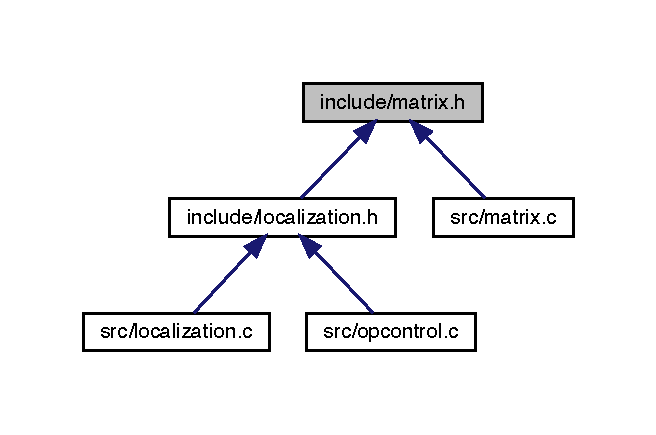
\includegraphics[width=315pt]{matrix_8h__dep__incl}
\end{center}
\end{figure}
\subsubsection*{Data Structures}
\begin{DoxyCompactItemize}
\item 
struct \textbf{ \+\_\+matrix}
\end{DoxyCompactItemize}
\subsubsection*{Typedefs}
\begin{DoxyCompactItemize}
\item 
typedef struct \textbf{ \+\_\+matrix} \textbf{ matrix}
\end{DoxyCompactItemize}
\subsubsection*{Functions}
\begin{DoxyCompactItemize}
\item 
void \textbf{ assert} (int assertion, const char $\ast$message)
\begin{DoxyCompactList}\small\item\em Asserts a condition is true. \end{DoxyCompactList}\item 
\textbf{ matrix} $\ast$ \textbf{ copy\+Matrix} (\textbf{ matrix} $\ast$m)
\begin{DoxyCompactList}\small\item\em Copies a matrix. This function uses scale\+Matrix, because scaling matrix by 1 is the same as a copy. \end{DoxyCompactList}\item 
\textbf{ matrix} $\ast$ \textbf{ covariance\+Matrix} (\textbf{ matrix} $\ast$m)
\begin{DoxyCompactList}\small\item\em returns the covariance of the matrix \end{DoxyCompactList}\item 
\textbf{ matrix} $\ast$ \textbf{ dot\+Diagonal\+Matrix} (\textbf{ matrix} $\ast$a, \textbf{ matrix} $\ast$b)
\begin{DoxyCompactList}\small\item\em performs a diagonial matrix dot product. Given a two matrices (or the same matrix twice) with identical widths and heights, this method returns a 1 by a-\/$>$height matrix of the cross product of each matrix along the diagonal. \end{DoxyCompactList}\item 
\textbf{ matrix} $\ast$ \textbf{ dot\+Product\+Matrix} (\textbf{ matrix} $\ast$a, \textbf{ matrix} $\ast$b)
\begin{DoxyCompactList}\small\item\em returns the matrix dot product. Given a two matrices (or the same matrix twice) with identical widths and different heights, this method returns a a-\/$>$height by b-\/$>$height matrix of the cross product of each matrix. \end{DoxyCompactList}\item 
void \textbf{ free\+Matrix} (\textbf{ matrix} $\ast$m)
\begin{DoxyCompactList}\small\item\em Frees the resources of a matrix. \end{DoxyCompactList}\item 
\textbf{ matrix} $\ast$ \textbf{ identity\+Matrix} (int n)
\begin{DoxyCompactList}\small\item\em Returns an identity matrix of size n by n. \end{DoxyCompactList}\item 
\textbf{ matrix} $\ast$ \textbf{ make\+Matrix} (int width, int height)
\begin{DoxyCompactList}\small\item\em Makes a matrix with a width and height parameters. \end{DoxyCompactList}\item 
\textbf{ matrix} $\ast$ \textbf{ mean\+Matrix} (\textbf{ matrix} $\ast$m)
\begin{DoxyCompactList}\small\item\em Given an \char`\"{}m rows by n columns\char`\"{} matrix, return a matrix where each element represents the mean of that full column.  the matrix. \end{DoxyCompactList}\item 
\textbf{ matrix} $\ast$ \textbf{ multiply\+Matrix} (\textbf{ matrix} $\ast$a, \textbf{ matrix} $\ast$b)
\begin{DoxyCompactList}\small\item\em Given a two matrices, returns the multiplication of the two. \end{DoxyCompactList}\item 
void \textbf{ print\+Matrix} (\textbf{ matrix} $\ast$m)
\begin{DoxyCompactList}\small\item\em Prints a matrix. \end{DoxyCompactList}\item 
void \textbf{ row\+Swap} (\textbf{ matrix} $\ast$a, int p, int q)
\begin{DoxyCompactList}\small\item\em swaps the rows of a matrix. This method changes the input matrix. Given a matrix, this algorithm will swap rows p and q, provided that p and q are less than or equal to the height of matrix A and p and q are different values. \end{DoxyCompactList}\item 
\textbf{ matrix} $\ast$ \textbf{ scale\+Matrix} (\textbf{ matrix} $\ast$m, double value)
\begin{DoxyCompactList}\small\item\em scales a matrix. \end{DoxyCompactList}\item 
double \textbf{ trace\+Matrix} (\textbf{ matrix} $\ast$m)
\begin{DoxyCompactList}\small\item\em Given an \char`\"{}m rows by n columns\char`\"{} matrix. \end{DoxyCompactList}\item 
\textbf{ matrix} $\ast$ \textbf{ transpose\+Matrix} (\textbf{ matrix} $\ast$m)
\begin{DoxyCompactList}\small\item\em returns the transpose matrix. \end{DoxyCompactList}\end{DoxyCompactItemize}


\subsubsection{Detailed Description}
Various Matrix operations.

None of the matrix operations below change the input matrices if an input is required. They all return a new matrix with the new changes. Because memory issues are so prevelant, be sure to use the  function to reclaim some of that memory. 



Definition in file \textbf{ matrix.\+h}.



\subsubsection{Typedef Documentation}
\mbox{\label{matrix_8h_abc75382643898dd572498a574bf891c7}} 
\index{matrix.\+h@{matrix.\+h}!matrix@{matrix}}
\index{matrix@{matrix}!matrix.\+h@{matrix.\+h}}
\paragraph{matrix}
{\footnotesize\ttfamily typedef struct \textbf{ \+\_\+matrix}  \textbf{ matrix}}

A struct representing a matrix 

\subsubsection{Function Documentation}
\mbox{\label{matrix_8h_a8e41e30382335ea89f90b72db0b44d6f}} 
\index{matrix.\+h@{matrix.\+h}!assert@{assert}}
\index{assert@{assert}!matrix.\+h@{matrix.\+h}}
\paragraph{assert()}
{\footnotesize\ttfamily void assert (\begin{DoxyParamCaption}\item[{int}]{assertion,  }\item[{const char $\ast$}]{message }\end{DoxyParamCaption})}



Asserts a condition is true. 

If the assertion is non-\/zero (i.\+e. true), then it returns. If the assertion is zero (i.\+e. false), then it display the string and aborts the program. This is ment to act like Python\textquotesingle{}s assert keyword. 

Definition at line \textbf{ 14} of file \textbf{ matrix.\+c}.



References \textbf{ fprintf()}.



Referenced by \textbf{ covariance\+Matrix()}, \textbf{ dot\+Diagonal\+Matrix()}, \textbf{ dot\+Product\+Matrix()}, \textbf{ identity\+Matrix()}, \textbf{ make\+Matrix()}, \textbf{ mean\+Matrix()}, \textbf{ multiply\+Matrix()}, and \textbf{ row\+Swap()}.


\begin{DoxyCode}
00014                                                 \{
00015     \textcolor{keywordflow}{if} (assertion == 0) \{
00016         fprintf(stderr, \textcolor{stringliteral}{"%s\(\backslash\)n"}, message);
00017         exit(1);
00018     \}
00019 \}
\end{DoxyCode}
Here is the call graph for this function\+:\nopagebreak
\begin{figure}[H]
\begin{center}
\leavevmode
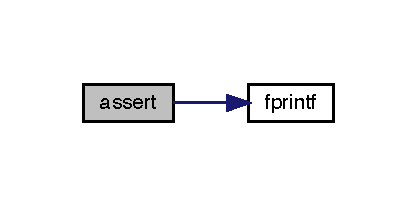
\includegraphics[width=200pt]{matrix_8h_a8e41e30382335ea89f90b72db0b44d6f_cgraph}
\end{center}
\end{figure}
Here is the caller graph for this function\+:\nopagebreak
\begin{figure}[H]
\begin{center}
\leavevmode
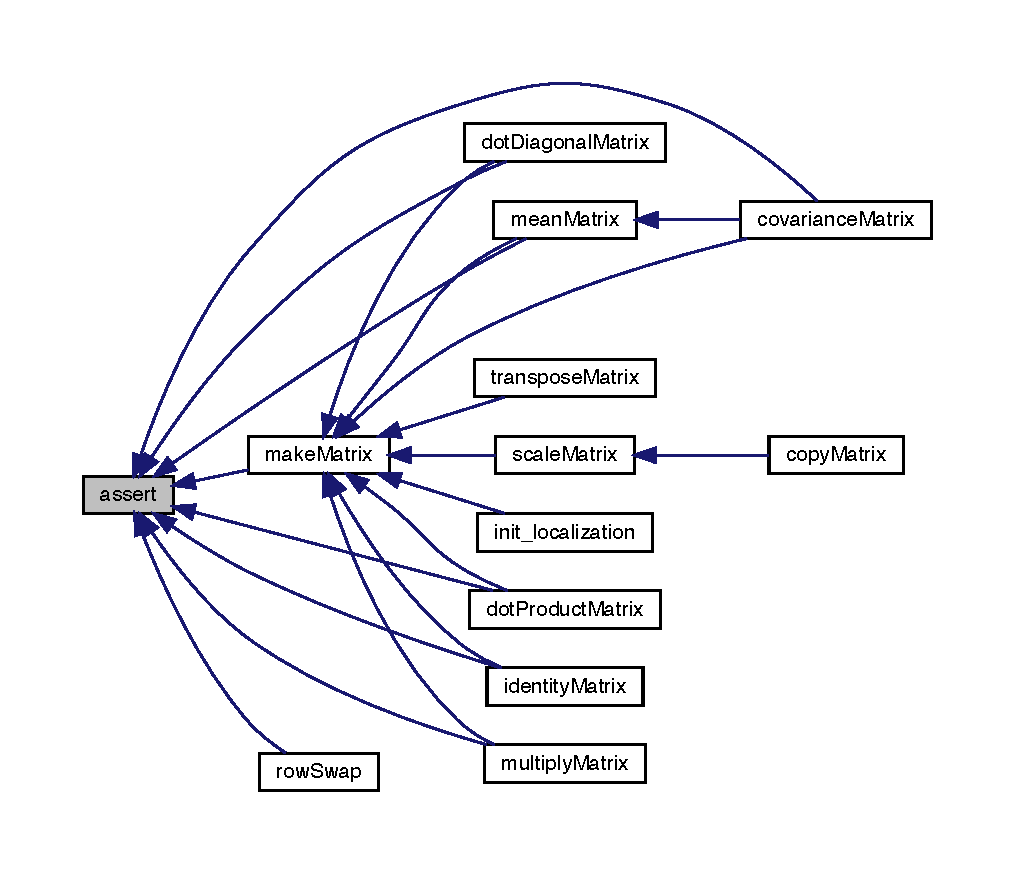
\includegraphics[width=350pt]{matrix_8h_a8e41e30382335ea89f90b72db0b44d6f_icgraph}
\end{center}
\end{figure}
\mbox{\label{matrix_8h_abbb8d2d20c2dd53a2269d017a336668f}} 
\index{matrix.\+h@{matrix.\+h}!copy\+Matrix@{copy\+Matrix}}
\index{copy\+Matrix@{copy\+Matrix}!matrix.\+h@{matrix.\+h}}
\paragraph{copy\+Matrix()}
{\footnotesize\ttfamily \textbf{ matrix}$\ast$ copy\+Matrix (\begin{DoxyParamCaption}\item[{\textbf{ matrix} $\ast$}]{m }\end{DoxyParamCaption})}



Copies a matrix. This function uses scale\+Matrix, because scaling matrix by 1 is the same as a copy. 


\begin{DoxyParams}{Parameters}
{\em m} & a pointer to the matrix \\
\hline
\end{DoxyParams}
\begin{DoxyReturn}{Returns}
a copied matrix 
\end{DoxyReturn}


Definition at line \textbf{ 52} of file \textbf{ matrix.\+c}.



References \textbf{ scale\+Matrix()}.


\begin{DoxyCode}
00052                               \{
00053     \textcolor{keywordflow}{return} scaleMatrix(m, 1);
00054 \}
\end{DoxyCode}
Here is the call graph for this function\+:\nopagebreak
\begin{figure}[H]
\begin{center}
\leavevmode
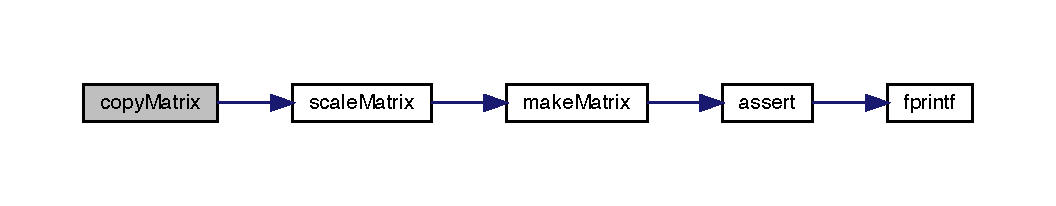
\includegraphics[width=350pt]{matrix_8h_abbb8d2d20c2dd53a2269d017a336668f_cgraph}
\end{center}
\end{figure}
\mbox{\label{matrix_8h_ae6dab569959c360cf165136a3b625edd}} 
\index{matrix.\+h@{matrix.\+h}!covariance\+Matrix@{covariance\+Matrix}}
\index{covariance\+Matrix@{covariance\+Matrix}!matrix.\+h@{matrix.\+h}}
\paragraph{covariance\+Matrix()}
{\footnotesize\ttfamily \textbf{ matrix}$\ast$ covariance\+Matrix (\begin{DoxyParamCaption}\item[{\textbf{ matrix} $\ast$}]{m }\end{DoxyParamCaption})}



returns the covariance of the matrix 


\begin{DoxyParams}{Parameters}
{\em the} & matrix \\
\hline
\end{DoxyParams}
\begin{DoxyReturn}{Returns}
a matrix with n row and n columns, where each element represents covariance of 2 columns. 
\end{DoxyReturn}


Definition at line \textbf{ 168} of file \textbf{ matrix.\+c}.



References \textbf{ assert()}, \textbf{ \+\_\+matrix\+::data}, \textbf{ free\+Matrix()}, \textbf{ \+\_\+matrix\+::height}, \textbf{ make\+Matrix()}, \textbf{ mean\+Matrix()}, and \textbf{ \+\_\+matrix\+::width}.


\begin{DoxyCode}
00168                                     \{
00169     \textcolor{keywordtype}{int} i, j, k = 0;
00170     matrix* out;
00171     matrix* mean;
00172     \textcolor{keywordtype}{double}* ptrA;
00173     \textcolor{keywordtype}{double}* ptrB;
00174     \textcolor{keywordtype}{double}* ptrOut;
00175 
00176     assert(m->height > 1, \textcolor{stringliteral}{"Height of matrix cannot be zero or one."});
00177 
00178     mean = meanMatrix(m);
00179     out = makeMatrix(m->width, m->width);
00180     ptrOut = out->data;
00181 
00182     \textcolor{keywordflow}{for} (i = 0; i < m->width; i++) \{
00183         \textcolor{keywordflow}{for} (j = 0; j < m->width; j++) \{
00184              ptrA = &m->data[i];
00185              ptrB = &m->data[j];
00186              *ptrOut = 0.0;
00187              \textcolor{keywordflow}{for} (k = 0; k < m->height; k++) \{
00188                  *ptrOut += (*ptrA - mean->data[i]) * (*ptrB - mean->data[j]);
00189                  ptrA += m->width;
00190                  ptrB += m->width;
00191              \}
00192              *ptrOut /= m->height - 1;
00193              ptrOut++;
00194         \}
00195     \}
00196 
00197     freeMatrix(mean);
00198     \textcolor{keywordflow}{return} out;
00199 \}
\end{DoxyCode}
Here is the call graph for this function\+:\nopagebreak
\begin{figure}[H]
\begin{center}
\leavevmode
\includegraphics[width=350pt]{matrix_8h_ae6dab569959c360cf165136a3b625edd_cgraph}
\end{center}
\end{figure}
\mbox{\label{matrix_8h_af49b525d7476c365833db9acd975e3a5}} 
\index{matrix.\+h@{matrix.\+h}!dot\+Diagonal\+Matrix@{dot\+Diagonal\+Matrix}}
\index{dot\+Diagonal\+Matrix@{dot\+Diagonal\+Matrix}!matrix.\+h@{matrix.\+h}}
\paragraph{dot\+Diagonal\+Matrix()}
{\footnotesize\ttfamily \textbf{ matrix}$\ast$ dot\+Diagonal\+Matrix (\begin{DoxyParamCaption}\item[{\textbf{ matrix} $\ast$}]{a,  }\item[{\textbf{ matrix} $\ast$}]{b }\end{DoxyParamCaption})}



performs a diagonial matrix dot product. Given a two matrices (or the same matrix twice) with identical widths and heights, this method returns a 1 by a-\/$>$height matrix of the cross product of each matrix along the diagonal. 

Dot product is essentially the sum-\/of-\/squares of two vectors.

If the second paramter is N\+U\+LL, it is assumed that we are performing a cross product with itself. 
\begin{DoxyParams}{Parameters}
{\em a} & the first matrix \\
\hline
{\em b} & the second matrix \\
\hline
\end{DoxyParams}
\begin{DoxyReturn}{Returns}
the matrix result 
\end{DoxyReturn}


Definition at line \textbf{ 385} of file \textbf{ matrix.\+c}.



References \textbf{ assert()}, \textbf{ \+\_\+matrix\+::data}, \textbf{ \+\_\+matrix\+::height}, \textbf{ make\+Matrix()}, and \textbf{ \+\_\+matrix\+::width}.


\begin{DoxyCode}
00385                                                 \{
00386     matrix* out;
00387     \textcolor{keywordtype}{double}* ptrOut;
00388     \textcolor{keywordtype}{double}* ptrA;
00389     \textcolor{keywordtype}{double}* ptrB;
00390     \textcolor{keywordtype}{int} i, j;
00391 
00392     \textcolor{keywordflow}{if} (b != NULL) \{
00393         assert(a->width == b->width && a->height == b->height, \textcolor{stringliteral}{"Matrices must be of the same
       dimensionality."});
00394     \}
00395 
00396     \textcolor{comment}{// Are we computing the sum of squares of the same matrix?}
00397     \textcolor{keywordflow}{if} (a == b || b == NULL) \{
00398         b = a; \textcolor{comment}{// May not appear safe, but we can do this without risk of losing b.}
00399     \}
00400 
00401     out = makeMatrix(1, a->height);
00402     ptrOut = out->data;
00403     ptrA = a->data;
00404     ptrB = b->data;
00405 
00406     \textcolor{keywordflow}{for} (i = 0; i < a->height; i++) \{
00407         *ptrOut = 0;
00408         \textcolor{keywordflow}{for} (j = 0; j < a->width; j++) \{
00409             *ptrOut += *ptrA * *ptrB;
00410             ptrA++;
00411             ptrB++;
00412         \}
00413         ptrOut++;
00414     \}
00415 
00416     \textcolor{keywordflow}{return} out;
00417 \}
\end{DoxyCode}
Here is the call graph for this function\+:\nopagebreak
\begin{figure}[H]
\begin{center}
\leavevmode
\includegraphics[width=350pt]{matrix_8h_af49b525d7476c365833db9acd975e3a5_cgraph}
\end{center}
\end{figure}
\mbox{\label{matrix_8h_a0b568a64e81a56779c2141b424475976}} 
\index{matrix.\+h@{matrix.\+h}!dot\+Product\+Matrix@{dot\+Product\+Matrix}}
\index{dot\+Product\+Matrix@{dot\+Product\+Matrix}!matrix.\+h@{matrix.\+h}}
\paragraph{dot\+Product\+Matrix()}
{\footnotesize\ttfamily \textbf{ matrix}$\ast$ dot\+Product\+Matrix (\begin{DoxyParamCaption}\item[{\textbf{ matrix} $\ast$}]{a,  }\item[{\textbf{ matrix} $\ast$}]{b }\end{DoxyParamCaption})}



returns the matrix dot product. Given a two matrices (or the same matrix twice) with identical widths and different heights, this method returns a a-\/$>$height by b-\/$>$height matrix of the cross product of each matrix. 

Dot product is essentially the sum-\/of-\/squares of two vectors.

Also, if the second paramter is N\+U\+LL, it is assumed that we are performing a cross product with itself. 
\begin{DoxyParams}{Parameters}
{\em a} & the first matrix \\
\hline
{\em the} & second matrix \\
\hline
\end{DoxyParams}
\begin{DoxyReturn}{Returns}
the result of the dot product 
\end{DoxyReturn}


Definition at line \textbf{ 333} of file \textbf{ matrix.\+c}.



References \textbf{ assert()}, \textbf{ \+\_\+matrix\+::data}, \textbf{ \+\_\+matrix\+::height}, \textbf{ make\+Matrix()}, and \textbf{ \+\_\+matrix\+::width}.


\begin{DoxyCode}
00333                                                \{
00334     matrix* out;
00335     \textcolor{keywordtype}{double}* ptrOut;
00336     \textcolor{keywordtype}{double}* ptrA;
00337     \textcolor{keywordtype}{double}* ptrB;
00338     \textcolor{keywordtype}{int} i, j, k;
00339 
00340     \textcolor{keywordflow}{if} (b != NULL) \{
00341         assert(a->width == b->width, \textcolor{stringliteral}{"Matrices must be of the same dimensionality."});
00342     \}
00343 
00344     \textcolor{comment}{// Are we computing the sum of squares of the same matrix?}
00345     \textcolor{keywordflow}{if} (a == b || b == NULL) \{
00346         b = a; \textcolor{comment}{// May not appear safe, but we can do this without risk of losing b.}
00347     \}
00348 
00349     out = makeMatrix(b->height, a->height);
00350     ptrOut = out->data;
00351 
00352     \textcolor{keywordflow}{for} (i = 0; i < a->height; i++) \{
00353         ptrB = b->data;
00354 
00355         \textcolor{keywordflow}{for} (j = 0; j < b->height; j++) \{
00356             ptrA = &a->data[ i * a->width ];
00357 
00358             *ptrOut = 0;
00359             \textcolor{keywordflow}{for} (k = 0; k < a->width; k++) \{
00360                 *ptrOut += *ptrA * *ptrB;
00361                 ptrA++;
00362                 ptrB++;
00363             \}
00364             ptrOut++;
00365         \}
00366     \}
00367 
00368     \textcolor{keywordflow}{return} out;
00369 \}
\end{DoxyCode}
Here is the call graph for this function\+:\nopagebreak
\begin{figure}[H]
\begin{center}
\leavevmode
\includegraphics[width=350pt]{matrix_8h_a0b568a64e81a56779c2141b424475976_cgraph}
\end{center}
\end{figure}
\mbox{\label{matrix_8h_ae98365c910e9d688d2bdedec50d89a6b}} 
\index{matrix.\+h@{matrix.\+h}!free\+Matrix@{free\+Matrix}}
\index{free\+Matrix@{free\+Matrix}!matrix.\+h@{matrix.\+h}}
\paragraph{free\+Matrix()}
{\footnotesize\ttfamily void free\+Matrix (\begin{DoxyParamCaption}\item[{\textbf{ matrix} $\ast$}]{m }\end{DoxyParamCaption})}



Frees the resources of a matrix. 


\begin{DoxyParams}{Parameters}
{\em the} & matrix to free \\
\hline
\end{DoxyParams}


Definition at line \textbf{ 60} of file \textbf{ matrix.\+c}.



References \textbf{ \+\_\+matrix\+::data}.



Referenced by \textbf{ covariance\+Matrix()}.


\begin{DoxyCode}
00060                            \{
00061     \textcolor{keywordflow}{if} (m != NULL) \{
00062         \textcolor{keywordflow}{if} (m->data != NULL) \{
00063             free(m->data);
00064             m->data = NULL;
00065         \}
00066         free(m);
00067     \}
00068     \textcolor{keywordflow}{return};
00069 \}
\end{DoxyCode}
Here is the caller graph for this function\+:\nopagebreak
\begin{figure}[H]
\begin{center}
\leavevmode
\includegraphics[width=268pt]{matrix_8h_ae98365c910e9d688d2bdedec50d89a6b_icgraph}
\end{center}
\end{figure}
\mbox{\label{matrix_8h_aa3f5e409b1641373be7cf7284e216d1a}} 
\index{matrix.\+h@{matrix.\+h}!identity\+Matrix@{identity\+Matrix}}
\index{identity\+Matrix@{identity\+Matrix}!matrix.\+h@{matrix.\+h}}
\paragraph{identity\+Matrix()}
{\footnotesize\ttfamily \textbf{ matrix}$\ast$ identity\+Matrix (\begin{DoxyParamCaption}\item[{int}]{n }\end{DoxyParamCaption})}



Returns an identity matrix of size n by n. 


\begin{DoxyParams}{Parameters}
{\em n} & the input matrix. parameter.\\
\hline
{\em n} & the input matrix. \\
\hline
\end{DoxyParams}
\begin{DoxyReturn}{Returns}
the identity matrix parameter. 
\end{DoxyReturn}


Definition at line \textbf{ 94} of file \textbf{ matrix.\+c}.



References \textbf{ assert()}, \textbf{ \+\_\+matrix\+::data}, and \textbf{ make\+Matrix()}.


\begin{DoxyCode}
00094                               \{
00095     \textcolor{keywordtype}{int} i;
00096     matrix *out;
00097     \textcolor{keywordtype}{double}* ptr;
00098 
00099     assert(n > 0, \textcolor{stringliteral}{"Identity matrix must have value greater than zero."});
00100 
00101     out = makeMatrix(n, n);
00102     ptr = out->data;
00103     \textcolor{keywordflow}{for} (i = 0; i < n; i++) \{
00104         *ptr = 1.0;
00105         ptr += n + 1;
00106     \}
00107 
00108     \textcolor{keywordflow}{return} out;
00109 \}
\end{DoxyCode}
Here is the call graph for this function\+:\nopagebreak
\begin{figure}[H]
\begin{center}
\leavevmode
\includegraphics[width=350pt]{matrix_8h_aa3f5e409b1641373be7cf7284e216d1a_cgraph}
\end{center}
\end{figure}
\mbox{\label{matrix_8h_aae8b56c6fb44d9147b835f4006ca872c}} 
\index{matrix.\+h@{matrix.\+h}!make\+Matrix@{make\+Matrix}}
\index{make\+Matrix@{make\+Matrix}!matrix.\+h@{matrix.\+h}}
\paragraph{make\+Matrix()}
{\footnotesize\ttfamily \textbf{ matrix}$\ast$ make\+Matrix (\begin{DoxyParamCaption}\item[{int}]{width,  }\item[{int}]{height }\end{DoxyParamCaption})}



Makes a matrix with a width and height parameters. 


\begin{DoxyParams}{Parameters}
{\em width} & The width of the matrix \\
\hline
{\em height} & the height of the matrix \\
\hline
\end{DoxyParams}
\begin{DoxyReturn}{Returns}
the new matrix 
\end{DoxyReturn}


Definition at line \textbf{ 27} of file \textbf{ matrix.\+c}.



References \textbf{ assert()}, \textbf{ \+\_\+matrix\+::data}, \textbf{ \+\_\+matrix\+::height}, and \textbf{ \+\_\+matrix\+::width}.



Referenced by \textbf{ covariance\+Matrix()}, \textbf{ dot\+Diagonal\+Matrix()}, \textbf{ dot\+Product\+Matrix()}, \textbf{ identity\+Matrix()}, \textbf{ init\+\_\+localization()}, \textbf{ mean\+Matrix()}, \textbf{ multiply\+Matrix()}, \textbf{ scale\+Matrix()}, and \textbf{ transpose\+Matrix()}.


\begin{DoxyCode}
00027                                           \{
00028     matrix* out;
00029     assert(width > 0 && height > 0, \textcolor{stringliteral}{"New matrix must be at least a 1 by 1"});
00030     out = (matrix*) malloc(\textcolor{keyword}{sizeof}(matrix));
00031 
00032     assert(out != NULL, \textcolor{stringliteral}{"Out of memory."});
00033 
00034     out->width = width;
00035     out->height = height;
00036     out->data = (\textcolor{keywordtype}{double}*) malloc(\textcolor{keyword}{sizeof}(\textcolor{keywordtype}{double}) * width * height);
00037 
00038     assert(out->data != NULL, \textcolor{stringliteral}{"Out of memory."});
00039 
00040     memset(out->data, 0.0, width * height * \textcolor{keyword}{sizeof}(\textcolor{keywordtype}{double}));
00041 
00042     \textcolor{keywordflow}{return} out;
00043 \}
\end{DoxyCode}
Here is the call graph for this function\+:\nopagebreak
\begin{figure}[H]
\begin{center}
\leavevmode
\includegraphics[width=304pt]{matrix_8h_aae8b56c6fb44d9147b835f4006ca872c_cgraph}
\end{center}
\end{figure}
Here is the caller graph for this function\+:\nopagebreak
\begin{figure}[H]
\begin{center}
\leavevmode
\includegraphics[width=350pt]{matrix_8h_aae8b56c6fb44d9147b835f4006ca872c_icgraph}
\end{center}
\end{figure}
\mbox{\label{matrix_8h_ae4babf9b518a2d5d6b12776191e3b7de}} 
\index{matrix.\+h@{matrix.\+h}!mean\+Matrix@{mean\+Matrix}}
\index{mean\+Matrix@{mean\+Matrix}!matrix.\+h@{matrix.\+h}}
\paragraph{mean\+Matrix()}
{\footnotesize\ttfamily \textbf{ matrix}$\ast$ mean\+Matrix (\begin{DoxyParamCaption}\item[{\textbf{ matrix} $\ast$}]{m }\end{DoxyParamCaption})}



Given an \char`\"{}m rows by n columns\char`\"{} matrix, return a matrix where each element represents the mean of that full column.  the matrix. 

\begin{DoxyReturn}{Returns}
matrix with 1 row and n columns each element represents the mean of that full column. 
\end{DoxyReturn}


Definition at line \textbf{ 142} of file \textbf{ matrix.\+c}.



References \textbf{ assert()}, \textbf{ \+\_\+matrix\+::data}, \textbf{ \+\_\+matrix\+::height}, \textbf{ make\+Matrix()}, and \textbf{ \+\_\+matrix\+::width}.



Referenced by \textbf{ covariance\+Matrix()}.


\begin{DoxyCode}
00142                               \{
00143     \textcolor{keywordtype}{int} i, j;
00144     matrix* out;
00145 
00146     assert(m->height > 0, \textcolor{stringliteral}{"Height of matrix cannot be zero."});
00147 
00148     out = makeMatrix(m->width, 1);
00149 
00150     \textcolor{keywordflow}{for} (i = 0; i < m->width; i++) \{
00151         \textcolor{keywordtype}{double}* ptr;
00152         out->data[i] = 0.0;
00153         ptr = &m->data[i];
00154         \textcolor{keywordflow}{for} (j = 0; j < m->height; j++) \{
00155             out->data[i] += *ptr;
00156             ptr += out->width;
00157         \}
00158         out->data[i] /= (double) m->height;
00159     \}
00160     \textcolor{keywordflow}{return} out;
00161 \}
\end{DoxyCode}
Here is the call graph for this function\+:\nopagebreak
\begin{figure}[H]
\begin{center}
\leavevmode
\includegraphics[width=350pt]{matrix_8h_ae4babf9b518a2d5d6b12776191e3b7de_cgraph}
\end{center}
\end{figure}
Here is the caller graph for this function\+:\nopagebreak
\begin{figure}[H]
\begin{center}
\leavevmode
\includegraphics[width=276pt]{matrix_8h_ae4babf9b518a2d5d6b12776191e3b7de_icgraph}
\end{center}
\end{figure}
\mbox{\label{matrix_8h_a63ed5c518b34768e9ef8e9d5f7d0b534}} 
\index{matrix.\+h@{matrix.\+h}!multiply\+Matrix@{multiply\+Matrix}}
\index{multiply\+Matrix@{multiply\+Matrix}!matrix.\+h@{matrix.\+h}}
\paragraph{multiply\+Matrix()}
{\footnotesize\ttfamily \textbf{ matrix}$\ast$ multiply\+Matrix (\begin{DoxyParamCaption}\item[{\textbf{ matrix} $\ast$}]{a,  }\item[{\textbf{ matrix} $\ast$}]{b }\end{DoxyParamCaption})}



Given a two matrices, returns the multiplication of the two. 


\begin{DoxyParams}{Parameters}
{\em a} & the first matrix \\
\hline
{\em b} & the seconf matrix return the result of the multiplication \\
\hline
\end{DoxyParams}


Definition at line \textbf{ 230} of file \textbf{ matrix.\+c}.



References \textbf{ assert()}, \textbf{ \+\_\+matrix\+::data}, \textbf{ \+\_\+matrix\+::height}, \textbf{ make\+Matrix()}, and \textbf{ \+\_\+matrix\+::width}.


\begin{DoxyCode}
00230                                              \{
00231     \textcolor{keywordtype}{int} i, j, k;
00232     matrix* out;
00233     \textcolor{keywordtype}{double}* ptrOut;
00234     \textcolor{keywordtype}{double}* ptrA;
00235     \textcolor{keywordtype}{double}* ptrB;
00236 
00237     assert(a->width == b->height, \textcolor{stringliteral}{"Matrices have incorrect dimensions. a->width != b->height"});
00238 
00239     out = makeMatrix(b->width, a->height);
00240     ptrOut = out->data;
00241 
00242     \textcolor{keywordflow}{for} (i = 0; i < a->height; i++) \{
00243 
00244         \textcolor{keywordflow}{for} (j = 0; j < b->width; j++) \{
00245             ptrA = &a->data[ i * a->width ];
00246             ptrB = &b->data[ j ];
00247 
00248             *ptrOut = 0;
00249             \textcolor{keywordflow}{for} (k = 0; k < a->width; k++) \{
00250                 *ptrOut += *ptrA * *ptrB;
00251                 ptrA++;
00252                 ptrB += b->width;
00253             \}
00254             ptrOut++;
00255         \}
00256     \}
00257 
00258     \textcolor{keywordflow}{return} out;
00259 \}
\end{DoxyCode}
Here is the call graph for this function\+:\nopagebreak
\begin{figure}[H]
\begin{center}
\leavevmode
\includegraphics[width=350pt]{matrix_8h_a63ed5c518b34768e9ef8e9d5f7d0b534_cgraph}
\end{center}
\end{figure}
\mbox{\label{matrix_8h_a50ab2b1ac33d6993d93522fc4f30a051}} 
\index{matrix.\+h@{matrix.\+h}!print\+Matrix@{print\+Matrix}}
\index{print\+Matrix@{print\+Matrix}!matrix.\+h@{matrix.\+h}}
\paragraph{print\+Matrix()}
{\footnotesize\ttfamily void print\+Matrix (\begin{DoxyParamCaption}\item[{\textbf{ matrix} $\ast$}]{m }\end{DoxyParamCaption})}



Prints a matrix. 


\begin{DoxyParams}{Parameters}
{\em the} & matrix \\
\hline
\end{DoxyParams}


Definition at line \textbf{ 75} of file \textbf{ matrix.\+c}.



References \textbf{ \+\_\+matrix\+::data}, \textbf{ \+\_\+matrix\+::height}, \textbf{ printf()}, and \textbf{ \+\_\+matrix\+::width}.


\begin{DoxyCode}
00075                             \{
00076     \textcolor{keywordtype}{int} i, j;
00077     \textcolor{keywordtype}{double}* ptr = m->data;
00078     printf(\textcolor{stringliteral}{"%d %d\(\backslash\)n"}, m->width, m->height);
00079     \textcolor{keywordflow}{for} (i = 0; i < m->height; i++) \{
00080         \textcolor{keywordflow}{for} (j = 0; j < m->width; j++) \{
00081             printf(\textcolor{stringliteral}{" %9.6f"}, *(ptr++));
00082         \}
00083         printf(\textcolor{stringliteral}{"\(\backslash\)n"});
00084     \}
00085     \textcolor{keywordflow}{return};
00086 \}
\end{DoxyCode}
Here is the call graph for this function\+:\nopagebreak
\begin{figure}[H]
\begin{center}
\leavevmode
\includegraphics[width=217pt]{matrix_8h_a50ab2b1ac33d6993d93522fc4f30a051_cgraph}
\end{center}
\end{figure}
\mbox{\label{matrix_8h_acdd57777a972ce339153878fa917db14}} 
\index{matrix.\+h@{matrix.\+h}!row\+Swap@{row\+Swap}}
\index{row\+Swap@{row\+Swap}!matrix.\+h@{matrix.\+h}}
\paragraph{row\+Swap()}
{\footnotesize\ttfamily void row\+Swap (\begin{DoxyParamCaption}\item[{\textbf{ matrix} $\ast$}]{a,  }\item[{int}]{p,  }\item[{int}]{q }\end{DoxyParamCaption})}



swaps the rows of a matrix. This method changes the input matrix. Given a matrix, this algorithm will swap rows p and q, provided that p and q are less than or equal to the height of matrix A and p and q are different values. 


\begin{DoxyParams}{Parameters}
{\em the} & matrix to swap. This method changes the input matrix. \\
\hline
{\em the} & first row \\
\hline
{\em the} & second row \\
\hline
\end{DoxyParams}


Definition at line \textbf{ 290} of file \textbf{ matrix.\+c}.



References \textbf{ assert()}, \textbf{ \+\_\+matrix\+::data}, \textbf{ \+\_\+matrix\+::height}, and \textbf{ \+\_\+matrix\+::width}.


\begin{DoxyCode}
00290                                       \{
00291     \textcolor{keywordtype}{int} i;
00292     \textcolor{keywordtype}{double} temp;
00293     \textcolor{keywordtype}{double}* pRow;
00294     \textcolor{keywordtype}{double}* qRow;
00295 
00296     assert(a->height > 2, \textcolor{stringliteral}{"Matrix must have at least two rows to swap."});
00297     assert(p < a->height && q < a->height, \textcolor{stringliteral}{"Values p and q must be less than the height of the matrix."});
00298 
00299     \textcolor{comment}{// If p and q are equal, do nothing.}
00300     \textcolor{keywordflow}{if} (p == q) \{
00301         \textcolor{keywordflow}{return};
00302     \}
00303 
00304     pRow = a->data + (p * a->width);
00305     qRow = a->data + (q * a->width);
00306 
00307     \textcolor{comment}{// Swap!}
00308     \textcolor{keywordflow}{for} (i = 0; i < a->width; i++) \{
00309         temp = *pRow;
00310         *pRow = *qRow;
00311         *qRow = temp;
00312         pRow++;
00313         qRow++;
00314     \}
00315 
00316     \textcolor{keywordflow}{return};
00317 \}
\end{DoxyCode}
Here is the call graph for this function\+:\nopagebreak
\begin{figure}[H]
\begin{center}
\leavevmode
\includegraphics[width=293pt]{matrix_8h_acdd57777a972ce339153878fa917db14_cgraph}
\end{center}
\end{figure}
\mbox{\label{matrix_8h_a6b7faa6ba9ee987d0777d9d0bd0e7b32}} 
\index{matrix.\+h@{matrix.\+h}!scale\+Matrix@{scale\+Matrix}}
\index{scale\+Matrix@{scale\+Matrix}!matrix.\+h@{matrix.\+h}}
\paragraph{scale\+Matrix()}
{\footnotesize\ttfamily \textbf{ matrix}$\ast$ scale\+Matrix (\begin{DoxyParamCaption}\item[{\textbf{ matrix} $\ast$}]{m,  }\item[{double}]{value }\end{DoxyParamCaption})}



scales a matrix. 


\begin{DoxyParams}{Parameters}
{\em m} & the matrix to scale \\
\hline
{\em the} & value to scale by \\
\hline
\end{DoxyParams}
\begin{DoxyReturn}{Returns}
a new matrix where each element in the input matrix is multiplied by the scalar value 
\end{DoxyReturn}


Definition at line \textbf{ 268} of file \textbf{ matrix.\+c}.



References \textbf{ \+\_\+matrix\+::data}, \textbf{ \+\_\+matrix\+::height}, \textbf{ make\+Matrix()}, and \textbf{ \+\_\+matrix\+::width}.



Referenced by \textbf{ copy\+Matrix()}.


\begin{DoxyCode}
00268                                              \{
00269     \textcolor{keywordtype}{int} i, elements = m->width * m->height;
00270     matrix* out = makeMatrix(m->width, m->height);
00271     \textcolor{keywordtype}{double}* ptrM = m->data;
00272     \textcolor{keywordtype}{double}* ptrOut = out->data;
00273 
00274     \textcolor{keywordflow}{for} (i = 0; i < elements; i++) \{
00275         *(ptrOut++) = *(ptrM++) * value;
00276     \}
00277 
00278     \textcolor{keywordflow}{return} out;
00279 \}
\end{DoxyCode}
Here is the call graph for this function\+:\nopagebreak
\begin{figure}[H]
\begin{center}
\leavevmode
\includegraphics[width=350pt]{matrix_8h_a6b7faa6ba9ee987d0777d9d0bd0e7b32_cgraph}
\end{center}
\end{figure}
Here is the caller graph for this function\+:\nopagebreak
\begin{figure}[H]
\begin{center}
\leavevmode
\includegraphics[width=247pt]{matrix_8h_a6b7faa6ba9ee987d0777d9d0bd0e7b32_icgraph}
\end{center}
\end{figure}
\mbox{\label{matrix_8h_a4794df8b2032f961dd8b2d90276bc417}} 
\index{matrix.\+h@{matrix.\+h}!trace\+Matrix@{trace\+Matrix}}
\index{trace\+Matrix@{trace\+Matrix}!matrix.\+h@{matrix.\+h}}
\paragraph{trace\+Matrix()}
{\footnotesize\ttfamily double trace\+Matrix (\begin{DoxyParamCaption}\item[{\textbf{ matrix} $\ast$}]{m }\end{DoxyParamCaption})}



Given an \char`\"{}m rows by n columns\char`\"{} matrix. 

\begin{DoxyReturn}{Returns}
the sum of the elements along the diagonal.
\end{DoxyReturn}
Given an \char`\"{}m rows by n columns\char`\"{} matrix.

\begin{DoxyReturn}{Returns}
the sum of the elements along the diagonal. 
\end{DoxyReturn}


Definition at line \textbf{ 116} of file \textbf{ matrix.\+c}.



References \textbf{ \+\_\+matrix\+::data}, \textbf{ \+\_\+matrix\+::height}, and \textbf{ \+\_\+matrix\+::width}.


\begin{DoxyCode}
00116                               \{
00117     \textcolor{keywordtype}{int} i;
00118     \textcolor{keywordtype}{int} size;
00119     \textcolor{keywordtype}{double}* ptr = m->data;
00120     \textcolor{keywordtype}{double} sum = 0.0;
00121 
00122     \textcolor{keywordflow}{if} (m->height < m->width) \{
00123         size = m->height;
00124     \}
00125     \textcolor{keywordflow}{else} \{
00126         size = m->width;
00127     \}
00128 
00129     \textcolor{keywordflow}{for} (i = 0; i < size; i++) \{
00130         sum += *ptr;
00131         ptr += m->width + 1;
00132     \}
00133 
00134     \textcolor{keywordflow}{return} sum;
00135 \}
\end{DoxyCode}
\mbox{\label{matrix_8h_a2936260302742748b0639e8ec71d4d9f}} 
\index{matrix.\+h@{matrix.\+h}!transpose\+Matrix@{transpose\+Matrix}}
\index{transpose\+Matrix@{transpose\+Matrix}!matrix.\+h@{matrix.\+h}}
\paragraph{transpose\+Matrix()}
{\footnotesize\ttfamily \textbf{ matrix}$\ast$ transpose\+Matrix (\begin{DoxyParamCaption}\item[{\textbf{ matrix} $\ast$}]{m }\end{DoxyParamCaption})}



returns the transpose matrix. 


\begin{DoxyParams}{Parameters}
{\em the} & matrix to transpose. \\
\hline
\end{DoxyParams}
\begin{DoxyReturn}{Returns}
the transposed matrix. 
\end{DoxyReturn}


Definition at line \textbf{ 206} of file \textbf{ matrix.\+c}.



References \textbf{ \+\_\+matrix\+::data}, \textbf{ \+\_\+matrix\+::height}, \textbf{ make\+Matrix()}, and \textbf{ \+\_\+matrix\+::width}.


\begin{DoxyCode}
00206                                    \{
00207     matrix* out = makeMatrix(m->height, m->width);
00208     \textcolor{keywordtype}{double}* ptrM = m->data;
00209     \textcolor{keywordtype}{int} i, j;
00210 
00211     \textcolor{keywordflow}{for} (i = 0; i < m->height; i++) \{
00212         \textcolor{keywordtype}{double}* ptrOut;
00213         ptrOut = &out->data[i];
00214         \textcolor{keywordflow}{for} (j = 0; j < m->width; j++) \{
00215             *ptrOut = *ptrM;
00216             ptrM++;
00217             ptrOut += out->width;
00218         \}
00219     \}
00220 
00221     \textcolor{keywordflow}{return} out;
00222 \}
\end{DoxyCode}
Here is the call graph for this function\+:\nopagebreak
\begin{figure}[H]
\begin{center}
\leavevmode
\includegraphics[width=350pt]{matrix_8h_a2936260302742748b0639e8ec71d4d9f_cgraph}
\end{center}
\end{figure}

\subsection{matrix.\+h}
\label{matrix_8h_source}\index{include/matrix.\+h@{include/matrix.\+h}}

\begin{DoxyCode}
00001 
00010 \textcolor{preprocessor}{#ifndef \_MATRIX\_H\_}
00011 \textcolor{preprocessor}{#define \_MATRIX\_H\_}
00012 
00016 \textcolor{keyword}{typedef} \textcolor{keyword}{struct }_matrix \{
00017   \textcolor{keywordtype}{int} height;
00018   \textcolor{keywordtype}{int} width;
00019   \textcolor{keywordtype}{double} *data;
00020 \} matrix;
00021 
00030 \textcolor{keywordtype}{void} assert(\textcolor{keywordtype}{int} assertion, \textcolor{keyword}{const} \textcolor{keywordtype}{char} *message);
00031 
00035 matrix *makeMatrix(\textcolor{keywordtype}{int} width, \textcolor{keywordtype}{int} height);
00036 
00044 matrix *copyMatrix(matrix *m);
00045 
00050 \textcolor{keywordtype}{void} freeMatrix(matrix *m);
00051 
00056 \textcolor{keywordtype}{void} printMatrix(matrix *m);
00057 
00063 matrix *identityMatrix(\textcolor{keywordtype}{int} n);
00064 
00070 \textcolor{keywordtype}{double} traceMatrix(matrix *m);
00071 
00077 matrix *transposeMatrix(matrix *m);
00078 
00086 matrix *meanMatrix(matrix *m);
00087 
00094 matrix *multiplyMatrix(matrix *a, matrix *b);
00095 
00103 matrix *scaleMatrix(matrix *m, \textcolor{keywordtype}{double} value);
00104 
00111 matrix *covarianceMatrix(matrix *m);
00112 
00122 \textcolor{keywordtype}{void} rowSwap(matrix *a, \textcolor{keywordtype}{int} p, \textcolor{keywordtype}{int} q);
00137 matrix *dotProductMatrix(matrix *a, matrix *b);
00138 
00153 matrix *dotDiagonalMatrix(matrix *a, matrix *b);
00154 
00155 \textcolor{preprocessor}{#endif}
\end{DoxyCode}

\section{include/menu.h File Reference}
\label{menu_8h}\index{include/menu.\+h@{include/menu.\+h}}


Contains menu functionality and abstraction.  


{\ttfamily \#include \char`\"{}lcd.\+h\char`\"{}}\newline
{\ttfamily \#include \char`\"{}A\+P\+I.\+h\char`\"{}}\newline
{\ttfamily \#include $<$string.\+h$>$}\newline
{\ttfamily \#include $<$limits.\+h$>$}\newline
{\ttfamily \#include $<$float.\+h$>$}\newline
{\ttfamily \#include $<$vlib.\+h$>$}\newline
{\ttfamily \#include \char`\"{}log.\+h\char`\"{}}\newline
Include dependency graph for menu.\+h\+:\nopagebreak
\begin{figure}[H]
\begin{center}
\leavevmode
\includegraphics[width=350pt]{menu_8h__incl}
\end{center}
\end{figure}
This graph shows which files directly or indirectly include this file\+:\nopagebreak
\begin{figure}[H]
\begin{center}
\leavevmode
\includegraphics[width=216pt]{menu_8h__dep__incl}
\end{center}
\end{figure}
\subsection*{Data Structures}
\begin{DoxyCompactItemize}
\item 
struct \textbf{ menu\+\_\+t}
\begin{DoxyCompactList}\small\item\em Represents a specific instance of a menu. Will cause a memory leak if not deinitialized via denint\+\_\+menu. \end{DoxyCompactList}\end{DoxyCompactItemize}
\subsection*{Typedefs}
\begin{DoxyCompactItemize}
\item 
typedef struct \textbf{ menu\+\_\+t} \textbf{ menu\+\_\+t}
\begin{DoxyCompactList}\small\item\em Represents a specific instance of a menu. Will cause a memory leak if not deinitialized via denint\+\_\+menu. \end{DoxyCompactList}\end{DoxyCompactItemize}
\subsection*{Enumerations}
\begin{DoxyCompactItemize}
\item 
enum \textbf{ menu\+\_\+type} \{ \textbf{ I\+N\+T\+\_\+\+T\+Y\+PE}, 
\textbf{ F\+L\+O\+A\+T\+\_\+\+T\+Y\+PE}, 
\textbf{ S\+T\+R\+I\+N\+G\+\_\+\+T\+Y\+PE}
 \}\begin{DoxyCompactList}\small\item\em Represents the different types of menus. \end{DoxyCompactList}
\end{DoxyCompactItemize}
\subsection*{Functions}
\begin{DoxyCompactItemize}
\item 
static void \textbf{ calculate\+\_\+current\+\_\+display} (char $\ast$rtn, \textbf{ menu\+\_\+t} $\ast$menu)
\begin{DoxyCompactList}\small\item\em Static function that calculates the string from menu. \end{DoxyCompactList}\item 
static \textbf{ menu\+\_\+t} $\ast$ \textbf{ create\+\_\+menu} (enum \textbf{ menu\+\_\+type} type, const char $\ast$prompt)
\begin{DoxyCompactList}\small\item\em Static function that handles creation of menu. {\itshape  Menu must be freed or will cause memory leak {\itshape  }}\end{DoxyCompactList}\item 
void \textbf{ denint\+\_\+menu} (\textbf{ menu\+\_\+t} $\ast$menu)
\begin{DoxyCompactList}\small\item\em Destroys a menu {\itshape  Menu must be freed or will cause memory leak {\itshape  }}\end{DoxyCompactList}\item 
int \textbf{ display\+\_\+menu} (\textbf{ menu\+\_\+t} $\ast$menu)
\begin{DoxyCompactList}\small\item\em Displays a menu context, but does not display. {\itshape  Menu must be freed or will cause memory leak! {\itshape  Will exit if robot is enabled. This prevents menu from locking up system in even of a reset. }}\end{DoxyCompactList}\item 
\textbf{ menu\+\_\+t} $\ast$ \textbf{ init\+\_\+menu\+\_\+float} (enum \textbf{ menu\+\_\+type} type, float \textbf{ min}, float \textbf{ max}, float step, const char $\ast$prompt)
\begin{DoxyCompactList}\small\item\em Creates a menu context, but does not display. {\itshape  Menu must be freed or will cause memory leak! {\itshape  }}\end{DoxyCompactList}\item 
\textbf{ menu\+\_\+t} $\ast$ \textbf{ init\+\_\+menu\+\_\+int} (enum \textbf{ menu\+\_\+type} type, int \textbf{ min}, int \textbf{ max}, int step, const char $\ast$prompt)
\begin{DoxyCompactList}\small\item\em Creates a menu context, but does not display. {\itshape  Menu must be freed or will cause memory leak {\itshape  }}\end{DoxyCompactList}\item 
\textbf{ menu\+\_\+t} $\ast$ \textbf{ init\+\_\+menu\+\_\+var} (enum \textbf{ menu\+\_\+type} type, unsigned int nums, const char $\ast$prompt, char $\ast$options,...)
\begin{DoxyCompactList}\small\item\em Creates a menu context, but does not display. {\itshape  Menu must be freed or will cause memory leak {\itshape  }}\end{DoxyCompactList}\end{DoxyCompactItemize}


\subsection{Detailed Description}
Contains menu functionality and abstraction. 

\begin{DoxyAuthor}{Author}
Chris Jerrett 
\end{DoxyAuthor}
\begin{DoxyDate}{Date}
9/9/2017 
\end{DoxyDate}


Definition in file \textbf{ menu.\+h}.



\subsection{Typedef Documentation}
\mbox{\label{menu_8h_aac280f147a4bb94ab2f1a69eff76f751}} 
\index{menu.\+h@{menu.\+h}!menu\+\_\+t@{menu\+\_\+t}}
\index{menu\+\_\+t@{menu\+\_\+t}!menu.\+h@{menu.\+h}}
\subsubsection{menu\+\_\+t}
{\footnotesize\ttfamily typedef struct \textbf{ menu\+\_\+t}  \textbf{ menu\+\_\+t}}



Represents a specific instance of a menu. Will cause a memory leak if not deinitialized via denint\+\_\+menu. 

\begin{DoxyAuthor}{Author}
Chris Jerrett 
\end{DoxyAuthor}
\begin{DoxyDate}{Date}
9/8/17 
\end{DoxyDate}
\begin{DoxySeeAlso}{See also}
\doxyref{menu.\+h}{p.}{menu_8h} 

\doxyref{menu\+\_\+t}{p.}{structmenu__t} 

\doxyref{create\+\_\+menu}{p.}{menu_8c_aff4fd27ff7707295d91c67fa52a6b021} 

init\+\_\+menu 

\doxyref{display\+\_\+menu}{p.}{menu_8c_abfadedb104f89f672dd3045499975a71} 

\doxyref{menu\+\_\+type}{p.}{menu_8h_a6bbf4baf5018b0d76aab6c2e6bf85e62} 

\doxyref{denint\+\_\+menu}{p.}{menu_8c_a05a36619ac6c9ba4544eddb83ee2a50d} 
\end{DoxySeeAlso}


\subsection{Enumeration Type Documentation}
\mbox{\label{menu_8h_a6bbf4baf5018b0d76aab6c2e6bf85e62}} 
\index{menu.\+h@{menu.\+h}!menu\+\_\+type@{menu\+\_\+type}}
\index{menu\+\_\+type@{menu\+\_\+type}!menu.\+h@{menu.\+h}}
\subsubsection{menu\+\_\+type}
{\footnotesize\ttfamily enum \textbf{ menu\+\_\+type}}



Represents the different types of menus. 

\begin{DoxyAuthor}{Author}
Chris Jerrett 
\end{DoxyAuthor}
\begin{DoxyDate}{Date}
9/8/17 
\end{DoxyDate}
\begin{DoxySeeAlso}{See also}
\doxyref{menu.\+h}{p.}{menu_8h} 

\doxyref{menu\+\_\+t}{p.}{structmenu__t} 

\doxyref{create\+\_\+menu}{p.}{menu_8h_adcee778eac0edb821427d32949106dc5} 

init\+\_\+menu 

\doxyref{display\+\_\+menu}{p.}{menu_8h_abfadedb104f89f672dd3045499975a71} 

\doxyref{menu\+\_\+type}{p.}{menu_8h_a6bbf4baf5018b0d76aab6c2e6bf85e62} 
\end{DoxySeeAlso}
\begin{DoxyEnumFields}{Enumerator}
\raisebox{\heightof{T}}[0pt][0pt]{\index{I\+N\+T\+\_\+\+T\+Y\+PE@{I\+N\+T\+\_\+\+T\+Y\+PE}!menu.\+h@{menu.\+h}}\index{menu.\+h@{menu.\+h}!I\+N\+T\+\_\+\+T\+Y\+PE@{I\+N\+T\+\_\+\+T\+Y\+PE}}}\mbox{\label{menu_8h_a6bbf4baf5018b0d76aab6c2e6bf85e62a7fee88532b24b79bf2a88688a5d681d7}} 
I\+N\+T\+\_\+\+T\+Y\+PE&Menu type allowing user to select a integer. The integer type menu has a max, min and a step value. Each step is calculated. Will return the index of the selected value. Example\+: User goes forwards twice then it will return 2. \\
\hline

\raisebox{\heightof{T}}[0pt][0pt]{\index{F\+L\+O\+A\+T\+\_\+\+T\+Y\+PE@{F\+L\+O\+A\+T\+\_\+\+T\+Y\+PE}!menu.\+h@{menu.\+h}}\index{menu.\+h@{menu.\+h}!F\+L\+O\+A\+T\+\_\+\+T\+Y\+PE@{F\+L\+O\+A\+T\+\_\+\+T\+Y\+PE}}}\mbox{\label{menu_8h_a6bbf4baf5018b0d76aab6c2e6bf85e62ab2a272a88abadbaa481269e2506345c5}} 
F\+L\+O\+A\+T\+\_\+\+T\+Y\+PE&Menu type allowing user to select a float The float type menu has a max, min and a step value. Each step is calculated. Will return the index of the selected value. Example\+: User goes forwards twice then it will return 2. \\
\hline

\raisebox{\heightof{T}}[0pt][0pt]{\index{S\+T\+R\+I\+N\+G\+\_\+\+T\+Y\+PE@{S\+T\+R\+I\+N\+G\+\_\+\+T\+Y\+PE}!menu.\+h@{menu.\+h}}\index{menu.\+h@{menu.\+h}!S\+T\+R\+I\+N\+G\+\_\+\+T\+Y\+PE@{S\+T\+R\+I\+N\+G\+\_\+\+T\+Y\+PE}}}\mbox{\label{menu_8h_a6bbf4baf5018b0d76aab6c2e6bf85e62a7823190eb356a6edf2f33589f250053c}} 
S\+T\+R\+I\+N\+G\+\_\+\+T\+Y\+PE&Menu type allowing user to select a string from a array of strings. Will return the index of the selected value. Example\+: User goes forwards twice then it will return 2. \\
\hline

\end{DoxyEnumFields}


Definition at line \textbf{ 30} of file \textbf{ menu.\+h}.


\begin{DoxyCode}
00030                \{
00037   INT_TYPE,
00044   FLOAT_TYPE,
00050   STRING_TYPE
00051 \};
\end{DoxyCode}


\subsection{Function Documentation}
\mbox{\label{menu_8h_a0fb55c1213b23963d509b974d1254567}} 
\index{menu.\+h@{menu.\+h}!calculate\+\_\+current\+\_\+display@{calculate\+\_\+current\+\_\+display}}
\index{calculate\+\_\+current\+\_\+display@{calculate\+\_\+current\+\_\+display}!menu.\+h@{menu.\+h}}
\subsubsection{calculate\+\_\+current\+\_\+display()}
{\footnotesize\ttfamily static void calculate\+\_\+current\+\_\+display (\begin{DoxyParamCaption}\item[{char $\ast$}]{rtn,  }\item[{\textbf{ menu\+\_\+t} $\ast$}]{menu }\end{DoxyParamCaption})\hspace{0.3cm}{\ttfamily [static]}}



Static function that calculates the string from menu. 


\begin{DoxyParams}{Parameters}
{\em rtn} & the string to be written to \\
\hline
{\em menu} & the menu for prompt to be calculated from \\
\hline
\end{DoxyParams}
\begin{DoxyAuthor}{Author}
Chris Jerrett 
\end{DoxyAuthor}
\begin{DoxyDate}{Date}
9/8/17 
\end{DoxyDate}
\mbox{\label{menu_8h_adcee778eac0edb821427d32949106dc5}} 
\index{menu.\+h@{menu.\+h}!create\+\_\+menu@{create\+\_\+menu}}
\index{create\+\_\+menu@{create\+\_\+menu}!menu.\+h@{menu.\+h}}
\subsubsection{create\+\_\+menu()}
{\footnotesize\ttfamily static \textbf{ menu\+\_\+t}$\ast$ create\+\_\+menu (\begin{DoxyParamCaption}\item[{enum \textbf{ menu\+\_\+type}}]{type,  }\item[{const char $\ast$}]{prompt }\end{DoxyParamCaption})\hspace{0.3cm}{\ttfamily [static]}}



Static function that handles creation of menu. {\itshape  Menu must be freed or will cause memory leak {\itshape  }}

\begin{DoxyAuthor}{Author}
Chris Jerrett 
\end{DoxyAuthor}
\begin{DoxyDate}{Date}
9/8/17 
\end{DoxyDate}
\mbox{\label{menu_8h_a05a36619ac6c9ba4544eddb83ee2a50d}} 
\index{menu.\+h@{menu.\+h}!denint\+\_\+menu@{denint\+\_\+menu}}
\index{denint\+\_\+menu@{denint\+\_\+menu}!menu.\+h@{menu.\+h}}
\subsubsection{denint\+\_\+menu()}
{\footnotesize\ttfamily void denint\+\_\+menu (\begin{DoxyParamCaption}\item[{\textbf{ menu\+\_\+t} $\ast$}]{menu }\end{DoxyParamCaption})}



Destroys a menu {\itshape  Menu must be freed or will cause memory leak {\itshape  }}


\begin{DoxyParams}{Parameters}
{\em menu} & the menu to free \\
\hline
\end{DoxyParams}
\begin{DoxySeeAlso}{See also}
menu 
\end{DoxySeeAlso}
\begin{DoxyAuthor}{Author}
Chris Jerrett 
\end{DoxyAuthor}
\begin{DoxyDate}{Date}
9/8/17 
\end{DoxyDate}


Definition at line \textbf{ 163} of file \textbf{ menu.\+c}.



References \textbf{ menu\+\_\+t\+::options}, and \textbf{ menu\+\_\+t\+::prompt}.


\begin{DoxyCode}
00163                               \{
00164   free(menu->prompt);
00165   \textcolor{keywordflow}{if}(menu->options != NULL) free(menu->options);
00166   free(menu);
00167 \}
\end{DoxyCode}
\mbox{\label{menu_8h_abfadedb104f89f672dd3045499975a71}} 
\index{menu.\+h@{menu.\+h}!display\+\_\+menu@{display\+\_\+menu}}
\index{display\+\_\+menu@{display\+\_\+menu}!menu.\+h@{menu.\+h}}
\subsubsection{display\+\_\+menu()}
{\footnotesize\ttfamily int display\+\_\+menu (\begin{DoxyParamCaption}\item[{\textbf{ menu\+\_\+t} $\ast$}]{menu }\end{DoxyParamCaption})}



Displays a menu context, but does not display. {\itshape  Menu must be freed or will cause memory leak! {\itshape  Will exit if robot is enabled. This prevents menu from locking up system in even of a reset. }}


\begin{DoxyParams}{Parameters}
{\em menu} & the menu to display \\
\hline
\end{DoxyParams}
\begin{DoxySeeAlso}{See also}
\doxyref{menu\+\_\+type}{p.}{menu_8h_a6bbf4baf5018b0d76aab6c2e6bf85e62} 
\end{DoxySeeAlso}
\begin{DoxyAuthor}{Author}
Chris Jerrett 
\end{DoxyAuthor}
\begin{DoxyDate}{Date}
9/8/17 
\end{DoxyDate}


Definition at line \textbf{ 136} of file \textbf{ menu.\+c}.



References \textbf{ calculate\+\_\+current\+\_\+display()}, \textbf{ menu\+\_\+t\+::current}, \textbf{ lcd\+\_\+get\+\_\+pressed\+\_\+buttons()}, \textbf{ lcd\+\_\+print()}, \textbf{ P\+R\+E\+S\+S\+ED}, \textbf{ menu\+\_\+t\+::prompt}, \textbf{ R\+E\+L\+E\+A\+S\+ED}, and \textbf{ T\+O\+P\+\_\+\+R\+OW}.


\begin{DoxyCode}
00136                               \{
00137   lcd_print(TOP_ROW, menu->prompt);
00138   \textcolor{comment}{//Will exit if teleop or autonomous begin. This is extremely important if robot disconnects or resets.}
00139   \textcolor{keywordflow}{while}(lcd_get_pressed_buttons().middle == RELEASED && !isEnabled()) \{
00140     \textcolor{keywordtype}{char} val[16];
00141     calculate_current_display(val, menu);
00142 
00143     \textcolor{keywordflow}{if}(lcd_get_pressed_buttons().right == PRESSED) \{
00144       menu->current += 1;
00145     \}
00146     \textcolor{keywordflow}{if}(lcd_get_pressed_buttons().left == PRESSED) \{
00147       menu->current -= 1;
00148     \}
00149     delay(500);
00150   \}
00151   \textcolor{keywordflow}{return} menu->current;
00152 \}
\end{DoxyCode}
\mbox{\label{menu_8h_a5abb752733423805f59ef3b92e3c2e57}} 
\index{menu.\+h@{menu.\+h}!init\+\_\+menu\+\_\+float@{init\+\_\+menu\+\_\+float}}
\index{init\+\_\+menu\+\_\+float@{init\+\_\+menu\+\_\+float}!menu.\+h@{menu.\+h}}
\subsubsection{init\+\_\+menu\+\_\+float()}
{\footnotesize\ttfamily \textbf{ menu\+\_\+t}$\ast$ init\+\_\+menu\+\_\+float (\begin{DoxyParamCaption}\item[{enum \textbf{ menu\+\_\+type}}]{type,  }\item[{float}]{min,  }\item[{float}]{max,  }\item[{float}]{step,  }\item[{const char $\ast$}]{prompt }\end{DoxyParamCaption})}



Creates a menu context, but does not display. {\itshape  Menu must be freed or will cause memory leak! {\itshape  }}


\begin{DoxyParams}{Parameters}
{\em type} & the type of menu \\
\hline
\end{DoxyParams}
\begin{DoxySeeAlso}{See also}
\doxyref{menu\+\_\+type}{p.}{menu_8h_a6bbf4baf5018b0d76aab6c2e6bf85e62} 
\end{DoxySeeAlso}

\begin{DoxyParams}{Parameters}
{\em min} & the minimum value \\
\hline
{\em max} & the maximum value \\
\hline
{\em step} & the step value \\
\hline
{\em prompt} & the prompt to display to user \\
\hline
\end{DoxyParams}
\begin{DoxyAuthor}{Author}
Chris Jerrett 
\end{DoxyAuthor}
\begin{DoxyDate}{Date}
9/8/17 
\end{DoxyDate}


Definition at line \textbf{ 92} of file \textbf{ menu.\+c}.



References \textbf{ create\+\_\+menu()}, \textbf{ max()}, \textbf{ menu\+\_\+t\+::max\+\_\+f}, \textbf{ min()}, \textbf{ menu\+\_\+t\+::min\+\_\+f}, and \textbf{ menu\+\_\+t\+::step\+\_\+f}.


\begin{DoxyCode}
00092                                                                                                   \{
00093   menu_t* menu = create_menu(type, prompt);
00094   menu->min_f = min;
00095   menu->max_f = max;
00096   menu->step_f = step;
00097   \textcolor{keywordflow}{return} menu;
00098 \}
\end{DoxyCode}
\mbox{\label{menu_8h_ac8efedba760ec35ebf841ab19543ba5a}} 
\index{menu.\+h@{menu.\+h}!init\+\_\+menu\+\_\+int@{init\+\_\+menu\+\_\+int}}
\index{init\+\_\+menu\+\_\+int@{init\+\_\+menu\+\_\+int}!menu.\+h@{menu.\+h}}
\subsubsection{init\+\_\+menu\+\_\+int()}
{\footnotesize\ttfamily \textbf{ menu\+\_\+t}$\ast$ init\+\_\+menu\+\_\+int (\begin{DoxyParamCaption}\item[{enum \textbf{ menu\+\_\+type}}]{type,  }\item[{int}]{min,  }\item[{int}]{max,  }\item[{int}]{step,  }\item[{const char $\ast$}]{prompt }\end{DoxyParamCaption})}



Creates a menu context, but does not display. {\itshape  Menu must be freed or will cause memory leak {\itshape  }}


\begin{DoxyParams}{Parameters}
{\em type} & the type of menu \\
\hline
\end{DoxyParams}
\begin{DoxySeeAlso}{See also}
\doxyref{menu\+\_\+type}{p.}{menu_8h_a6bbf4baf5018b0d76aab6c2e6bf85e62} 
\end{DoxySeeAlso}

\begin{DoxyParams}{Parameters}
{\em min} & the minimum value \\
\hline
{\em max} & the maximum value \\
\hline
{\em step} & the step value \\
\hline
{\em prompt} & the prompt to display to user \\
\hline
\end{DoxyParams}
\begin{DoxyAuthor}{Author}
Chris Jerrett 
\end{DoxyAuthor}
\begin{DoxyDate}{Date}
9/8/17 
\end{DoxyDate}


Definition at line \textbf{ 71} of file \textbf{ menu.\+c}.



References \textbf{ create\+\_\+menu()}, \textbf{ max()}, \textbf{ menu\+\_\+t\+::max}, \textbf{ min()}, \textbf{ menu\+\_\+t\+::min}, and \textbf{ menu\+\_\+t\+::step}.


\begin{DoxyCode}
00071                                                                                           \{
00072   menu_t* menu = create_menu(type, prompt);
00073   menu->min = min;
00074   menu->max = max;
00075   menu->step = step;
00076   \textcolor{keywordflow}{return} menu;
00077 \}
\end{DoxyCode}
\mbox{\label{menu_8h_a3529988b0a7c12cb3f2ebb3cf5595594}} 
\index{menu.\+h@{menu.\+h}!init\+\_\+menu\+\_\+var@{init\+\_\+menu\+\_\+var}}
\index{init\+\_\+menu\+\_\+var@{init\+\_\+menu\+\_\+var}!menu.\+h@{menu.\+h}}
\subsubsection{init\+\_\+menu\+\_\+var()}
{\footnotesize\ttfamily \textbf{ menu\+\_\+t}$\ast$ init\+\_\+menu\+\_\+var (\begin{DoxyParamCaption}\item[{enum \textbf{ menu\+\_\+type}}]{type,  }\item[{unsigned int}]{nums,  }\item[{const char $\ast$}]{prompt,  }\item[{char $\ast$}]{options,  }\item[{}]{... }\end{DoxyParamCaption})}



Creates a menu context, but does not display. {\itshape  Menu must be freed or will cause memory leak {\itshape  }}


\begin{DoxyParams}{Parameters}
{\em type} & the type of menu \\
\hline
\end{DoxyParams}
\begin{DoxySeeAlso}{See also}
\doxyref{menu\+\_\+type}{p.}{menu_8h_a6bbf4baf5018b0d76aab6c2e6bf85e62} 
\end{DoxySeeAlso}

\begin{DoxyParams}{Parameters}
{\em nums} & the number of elements passed to function \\
\hline
{\em prompt} & the prompt to display to user \\
\hline
{\em options} & the options to display for user \\
\hline
\end{DoxyParams}
\begin{DoxyAuthor}{Author}
Chris Jerrett 
\end{DoxyAuthor}
\begin{DoxyDate}{Date}
9/8/17 
\end{DoxyDate}


Definition at line \textbf{ 44} of file \textbf{ menu.\+c}.



References \textbf{ create\+\_\+menu()}, \textbf{ menu\+\_\+t\+::length}, and \textbf{ menu\+\_\+t\+::options}.


\begin{DoxyCode}
00044                                                                                                     \{
00045   menu_t* menu = create_menu(type, prompt);
00046   va\_list values;
00047   \textcolor{keywordtype}{char} **options\_array = (\textcolor{keywordtype}{char}**)calloc(\textcolor{keyword}{sizeof}(\textcolor{keywordtype}{char}*), nums);
00048   va\_start(values, options);
00049   \textcolor{keywordflow}{for}(\textcolor{keywordtype}{unsigned} \textcolor{keywordtype}{int} i = 0; i < nums; i++)\{
00050     options\_array[i] = va\_arg(values, \textcolor{keywordtype}{char}*);
00051   \}
00052   va\_end(values);
00053   menu->options = options\_array;
00054   menu->length = nums;
00055   \textcolor{keywordflow}{return} menu;
00056 \}
\end{DoxyCode}

\subsection{menu.\+h}
\label{menu_8h_source}\index{include/menu.\+h@{include/menu.\+h}}

\begin{DoxyCode}
00001 
00008 \textcolor{preprocessor}{#ifndef \_MENU\_H\_}
00009 \textcolor{preprocessor}{#define \_MENU\_H\_}
00010 
00011 \textcolor{preprocessor}{#include "API.h"}
00012 \textcolor{preprocessor}{#include "lcd.h"}
00013 \textcolor{preprocessor}{#include <float.h>}
00014 \textcolor{preprocessor}{#include <limits.h>}
00015 \textcolor{preprocessor}{#include <string.h>}
00016 \textcolor{preprocessor}{#include <vlib.h>}
00017 \textcolor{preprocessor}{#include "log.h"}
00018 
00030 \textcolor{keyword}{enum} menu_type \{
00037   INT_TYPE,
00044   FLOAT_TYPE,
00050   STRING_TYPE
00051 \};
00052 
00066 \textcolor{keyword}{typedef} \textcolor{keyword}{struct }menu_t \{
00072   \textcolor{keyword}{enum} menu_type type;
00073 
00079   \textcolor{keywordtype}{char} **options;
00080 
00086   \textcolor{keywordtype}{unsigned} \textcolor{keywordtype}{int} length;
00087 
00094   \textcolor{keywordtype}{int} min;
00095 
00102   \textcolor{keywordtype}{int} max;
00103 
00111   \textcolor{keywordtype}{int} step;
00112 
00119   \textcolor{keywordtype}{float} min_f;
00120 
00127   \textcolor{keywordtype}{float} max_f;
00128 
00136   \textcolor{keywordtype}{float} step_f;
00142   \textcolor{keywordtype}{int} current;
00150   \textcolor{keywordtype}{char} *prompt;
00151 \} menu_t;
00152 
00165 menu_t *init_menu_var(\textcolor{keyword}{enum} menu_type type, \textcolor{keyword}{const} \textcolor{keywordtype}{char} *prompt, \textcolor{keywordtype}{int} nums, ...);
00166 
00180 menu_t *init_menu_int(\textcolor{keyword}{enum} menu_type type, \textcolor{keywordtype}{int} min, \textcolor{keywordtype}{int} max, \textcolor{keywordtype}{int} step,
00181                       \textcolor{keyword}{const} \textcolor{keywordtype}{char} *prompt);
00182 
00196 menu_t *init_menu_float(\textcolor{keyword}{enum} menu_type type, \textcolor{keywordtype}{float} min, \textcolor{keywordtype}{float} max, \textcolor{keywordtype}{float} step,
00197                         \textcolor{keyword}{const} \textcolor{keywordtype}{char} *prompt);
00198 
00209 \textcolor{keywordtype}{int} display_menu(menu_t *menu);
00210 
00220 \textcolor{keywordtype}{void} denint_menu(menu_t *menu);
00221 
00222 \textcolor{preprocessor}{#endif}
\end{DoxyCode}

\subsection{include/mobile\+\_\+goal\+\_\+intake.h File Reference}
\label{mobile__goal__intake_8h}\index{include/mobile\+\_\+goal\+\_\+intake.\+h@{include/mobile\+\_\+goal\+\_\+intake.\+h}}
{\ttfamily \#include \char`\"{}motor\+\_\+ports.\+h\char`\"{}}\newline
{\ttfamily \#include \char`\"{}controller.\+h\char`\"{}}\newline
{\ttfamily \#include \char`\"{}slew.\+h\char`\"{}}\newline
Include dependency graph for mobile\+\_\+goal\+\_\+intake.\+h\+:\nopagebreak
\begin{figure}[H]
\begin{center}
\leavevmode
\includegraphics[width=350pt]{mobile__goal__intake_8h__incl}
\end{center}
\end{figure}
This graph shows which files directly or indirectly include this file\+:\nopagebreak
\begin{figure}[H]
\begin{center}
\leavevmode
\includegraphics[width=306pt]{mobile__goal__intake_8h__dep__incl}
\end{center}
\end{figure}
\subsubsection*{Functions}
\begin{DoxyCompactItemize}
\item 
void \textbf{ update\+Intake} ()
\begin{DoxyCompactList}\small\item\em updates the mobile goal intake in teleop. \end{DoxyCompactList}\end{DoxyCompactItemize}


\subsubsection{Function Documentation}
\mbox{\label{mobile__goal__intake_8h_ad0232c21c5c1ffda603d2b7d61034118}} 
\index{mobile\+\_\+goal\+\_\+intake.\+h@{mobile\+\_\+goal\+\_\+intake.\+h}!update\+Intake@{update\+Intake}}
\index{update\+Intake@{update\+Intake}!mobile\+\_\+goal\+\_\+intake.\+h@{mobile\+\_\+goal\+\_\+intake.\+h}}
\paragraph{update\+Intake()}
{\footnotesize\ttfamily void update\+Intake (\begin{DoxyParamCaption}{ }\end{DoxyParamCaption})}



updates the mobile goal intake in teleop. 



Definition at line \textbf{ 16} of file \textbf{ mobile\+\_\+goal\+\_\+intake.\+c}.



References \textbf{ get\+\_\+mode()}, \textbf{ J\+O\+Y\+\_\+\+D\+O\+WN}, \textbf{ J\+O\+Y\+\_\+\+UP}, \textbf{ joystick\+Get\+Digital()}, \textbf{ lower\+\_\+intake()}, \textbf{ M\+A\+I\+N\+\_\+\+C\+O\+N\+T\+R\+O\+L\+L\+E\+R\+\_\+\+M\+O\+DE}, \textbf{ M\+A\+S\+T\+ER}, \textbf{ P\+A\+R\+T\+N\+ER}, \textbf{ P\+A\+R\+T\+N\+E\+R\+\_\+\+C\+O\+N\+T\+R\+O\+L\+L\+E\+R\+\_\+\+M\+O\+DE}, \textbf{ raise\+\_\+intake()}, and \textbf{ set\+\_\+intake\+\_\+motor()}.



Referenced by \textbf{ operator\+Control()}.


\begin{DoxyCode}
00016                     \{
00017   \textcolor{keywordflow}{if}(joystickGetDigital(MASTER, 7, JOY_UP) && (get_mode() == 
      MAIN_CONTROLLER_MODE)
00018   || joystickGetDigital(PARTNER, 6, JOY_UP) && get_mode() == 
      PARTNER_CONTROLLER_MODE) \{
00019     raise_intake();
00020   \}
00021   \textcolor{keywordflow}{else} \textcolor{keywordflow}{if}(joystickGetDigital(MASTER, 7, JOY_DOWN) && (get_mode() == 
      MAIN_CONTROLLER_MODE)
00022   || joystickGetDigital(PARTNER, 6, JOY_DOWN) && get_mode() == 
      PARTNER_CONTROLLER_MODE)\{
00023     lower_intake();
00024   \}
00025   \textcolor{keywordflow}{else} set_intake_motor(0);
00026 \}
\end{DoxyCode}
Here is the call graph for this function\+:\nopagebreak
\begin{figure}[H]
\begin{center}
\leavevmode
\includegraphics[width=350pt]{mobile__goal__intake_8h_ad0232c21c5c1ffda603d2b7d61034118_cgraph}
\end{center}
\end{figure}
Here is the caller graph for this function\+:\nopagebreak
\begin{figure}[H]
\begin{center}
\leavevmode
\includegraphics[width=275pt]{mobile__goal__intake_8h_ad0232c21c5c1ffda603d2b7d61034118_icgraph}
\end{center}
\end{figure}

\subsection{mobile\+\_\+goal\+\_\+intake.\+h}
\label{mobile__goal__intake_8h_source}\index{include/mobile\+\_\+goal\+\_\+intake.\+h@{include/mobile\+\_\+goal\+\_\+intake.\+h}}

\begin{DoxyCode}
00001 \textcolor{preprocessor}{#ifndef \_MOBLE\_GOAL\_INTAKE\_}
00002 \textcolor{preprocessor}{#define  \_MOBLE\_GOAL\_INTAKE\_}
00003 
00004 \textcolor{preprocessor}{#include "motor_ports.h"}
00005 \textcolor{preprocessor}{#include "controller.h"}
00006 \textcolor{preprocessor}{#include "slew.h"}
00007 
00011 \textcolor{keywordtype}{void} updateIntake();
00012 
00013 \textcolor{preprocessor}{#endif}
\end{DoxyCode}

\section{include/motor\+\_\+ports.h File Reference}
\label{motor__ports_8h}\index{include/motor\+\_\+ports.\+h@{include/motor\+\_\+ports.\+h}}


The motor port definitions

Macros for the different motors ports.  


This graph shows which files directly or indirectly include this file\+:\nopagebreak
\begin{figure}[H]
\begin{center}
\leavevmode
\includegraphics[width=350pt]{motor__ports_8h__dep__incl}
\end{center}
\end{figure}
\subsection*{Macros}
\begin{DoxyCompactItemize}
\item 
\#define \textbf{ \+\_\+\+M\+O\+T\+O\+R\+\_\+\+P\+O\+R\+T\+S\+\_\+\+H\+\_\+}
\item 
\#define \textbf{ C\+L\+A\+W\+\_\+\+M\+O\+T\+OR}~10
\item 
\#define \textbf{ I\+N\+T\+A\+K\+E\+\_\+\+M\+O\+T\+OR}~1
\item 
\#define \textbf{ M\+A\+X\+\_\+\+S\+P\+E\+ED}~127
\begin{DoxyCompactList}\small\item\em Max motor speed. \end{DoxyCompactList}\item 
\#define \textbf{ M\+I\+N\+\_\+\+S\+P\+E\+ED}~-\/127
\item 
\#define \textbf{ M\+O\+T\+O\+R\+\_\+\+B\+A\+C\+K\+\_\+\+L\+E\+FT}~5
\begin{DoxyCompactList}\small\item\em Back left drive motor of robot base. \end{DoxyCompactList}\item 
\#define \textbf{ M\+O\+T\+O\+R\+\_\+\+B\+A\+C\+K\+\_\+\+R\+I\+G\+HT}~4
\begin{DoxyCompactList}\small\item\em Back right drive motor of robot base. \end{DoxyCompactList}\item 
\#define \textbf{ M\+O\+T\+O\+R\+\_\+\+F\+R\+O\+N\+T\+\_\+\+L\+E\+FT}~7
\begin{DoxyCompactList}\small\item\em Front left drive motor of robot base. \end{DoxyCompactList}\item 
\#define \textbf{ M\+O\+T\+O\+R\+\_\+\+F\+R\+O\+N\+T\+\_\+\+R\+I\+G\+HT}~2
\begin{DoxyCompactList}\small\item\em Front right drive motor of robot base. \end{DoxyCompactList}\item 
\#define \textbf{ M\+O\+T\+O\+R\+\_\+\+L\+I\+F\+T\+\_\+\+B\+O\+T\+T\+O\+M\+\_\+\+L\+E\+FT}~9
\item 
\#define \textbf{ M\+O\+T\+O\+R\+\_\+\+L\+I\+F\+T\+\_\+\+B\+O\+T\+T\+O\+M\+\_\+\+R\+I\+G\+HT}~8
\item 
\#define \textbf{ M\+O\+T\+O\+R\+\_\+\+L\+I\+F\+T\+\_\+\+T\+O\+P\+\_\+\+L\+E\+FT}~9
\item 
\#define \textbf{ M\+O\+T\+O\+R\+\_\+\+L\+I\+F\+T\+\_\+\+T\+O\+P\+\_\+\+R\+I\+G\+HT}~8
\item 
\#define \textbf{ M\+O\+T\+O\+R\+\_\+\+M\+I\+D\+D\+L\+E\+\_\+\+L\+E\+FT}~6
\begin{DoxyCompactList}\small\item\em Middle left drive motor of robot base. \end{DoxyCompactList}\item 
\#define \textbf{ M\+O\+T\+O\+R\+\_\+\+M\+I\+D\+D\+L\+E\+\_\+\+R\+I\+G\+HT}~3
\begin{DoxyCompactList}\small\item\em Middle right drive motor of robot base. \end{DoxyCompactList}\end{DoxyCompactItemize}


\subsection{Detailed Description}
The motor port definitions

Macros for the different motors ports. 



Definition in file \textbf{ motor\+\_\+ports.\+h}.



\subsection{Macro Definition Documentation}
\mbox{\label{motor__ports_8h_a96b0e64c39730b0c4ca0d9e493bc0f58}} 
\index{motor\+\_\+ports.\+h@{motor\+\_\+ports.\+h}!\+\_\+\+M\+O\+T\+O\+R\+\_\+\+P\+O\+R\+T\+S\+\_\+\+H\+\_\+@{\+\_\+\+M\+O\+T\+O\+R\+\_\+\+P\+O\+R\+T\+S\+\_\+\+H\+\_\+}}
\index{\+\_\+\+M\+O\+T\+O\+R\+\_\+\+P\+O\+R\+T\+S\+\_\+\+H\+\_\+@{\+\_\+\+M\+O\+T\+O\+R\+\_\+\+P\+O\+R\+T\+S\+\_\+\+H\+\_\+}!motor\+\_\+ports.\+h@{motor\+\_\+ports.\+h}}
\subsubsection{\+\_\+\+M\+O\+T\+O\+R\+\_\+\+P\+O\+R\+T\+S\+\_\+\+H\+\_\+}
{\footnotesize\ttfamily \#define \+\_\+\+M\+O\+T\+O\+R\+\_\+\+P\+O\+R\+T\+S\+\_\+\+H\+\_\+}



Definition at line \textbf{ 7} of file \textbf{ motor\+\_\+ports.\+h}.

\mbox{\label{motor__ports_8h_aa3bcf05406f673f735df023643f347bb}} 
\index{motor\+\_\+ports.\+h@{motor\+\_\+ports.\+h}!C\+L\+A\+W\+\_\+\+M\+O\+T\+OR@{C\+L\+A\+W\+\_\+\+M\+O\+T\+OR}}
\index{C\+L\+A\+W\+\_\+\+M\+O\+T\+OR@{C\+L\+A\+W\+\_\+\+M\+O\+T\+OR}!motor\+\_\+ports.\+h@{motor\+\_\+ports.\+h}}
\subsubsection{C\+L\+A\+W\+\_\+\+M\+O\+T\+OR}
{\footnotesize\ttfamily \#define C\+L\+A\+W\+\_\+\+M\+O\+T\+OR~10}



Definition at line \textbf{ 61} of file \textbf{ motor\+\_\+ports.\+h}.



Referenced by \textbf{ close\+\_\+claw()}, \textbf{ open\+\_\+claw()}, and \textbf{ set\+\_\+claw\+\_\+motor()}.

\mbox{\label{motor__ports_8h_a2badb0c22cf65b0e81743c90de9a3b41}} 
\index{motor\+\_\+ports.\+h@{motor\+\_\+ports.\+h}!I\+N\+T\+A\+K\+E\+\_\+\+M\+O\+T\+OR@{I\+N\+T\+A\+K\+E\+\_\+\+M\+O\+T\+OR}}
\index{I\+N\+T\+A\+K\+E\+\_\+\+M\+O\+T\+OR@{I\+N\+T\+A\+K\+E\+\_\+\+M\+O\+T\+OR}!motor\+\_\+ports.\+h@{motor\+\_\+ports.\+h}}
\subsubsection{I\+N\+T\+A\+K\+E\+\_\+\+M\+O\+T\+OR}
{\footnotesize\ttfamily \#define I\+N\+T\+A\+K\+E\+\_\+\+M\+O\+T\+OR~1}



Definition at line \textbf{ 62} of file \textbf{ motor\+\_\+ports.\+h}.



Referenced by \textbf{ set\+\_\+intake\+\_\+motor()}.

\mbox{\label{motor__ports_8h_ac2cd96d53dd3ba6407db6766c3d92b26}} 
\index{motor\+\_\+ports.\+h@{motor\+\_\+ports.\+h}!M\+A\+X\+\_\+\+S\+P\+E\+ED@{M\+A\+X\+\_\+\+S\+P\+E\+ED}}
\index{M\+A\+X\+\_\+\+S\+P\+E\+ED@{M\+A\+X\+\_\+\+S\+P\+E\+ED}!motor\+\_\+ports.\+h@{motor\+\_\+ports.\+h}}
\subsubsection{M\+A\+X\+\_\+\+S\+P\+E\+ED}
{\footnotesize\ttfamily \#define M\+A\+X\+\_\+\+S\+P\+E\+ED~127}



Max motor speed. 



Definition at line \textbf{ 12} of file \textbf{ motor\+\_\+ports.\+h}.



Referenced by \textbf{ raise\+\_\+lifter()}.

\mbox{\label{motor__ports_8h_ad5f5efaa5cb771bd06da4bfe6046809e}} 
\index{motor\+\_\+ports.\+h@{motor\+\_\+ports.\+h}!M\+I\+N\+\_\+\+S\+P\+E\+ED@{M\+I\+N\+\_\+\+S\+P\+E\+ED}}
\index{M\+I\+N\+\_\+\+S\+P\+E\+ED@{M\+I\+N\+\_\+\+S\+P\+E\+ED}!motor\+\_\+ports.\+h@{motor\+\_\+ports.\+h}}
\subsubsection{M\+I\+N\+\_\+\+S\+P\+E\+ED}
{\footnotesize\ttfamily \#define M\+I\+N\+\_\+\+S\+P\+E\+ED~-\/127}



Definition at line \textbf{ 13} of file \textbf{ motor\+\_\+ports.\+h}.



Referenced by \textbf{ lower\+\_\+lifter()}.

\mbox{\label{motor__ports_8h_a36e9fda07b5cd4408170fe907b75a8b7}} 
\index{motor\+\_\+ports.\+h@{motor\+\_\+ports.\+h}!M\+O\+T\+O\+R\+\_\+\+B\+A\+C\+K\+\_\+\+L\+E\+FT@{M\+O\+T\+O\+R\+\_\+\+B\+A\+C\+K\+\_\+\+L\+E\+FT}}
\index{M\+O\+T\+O\+R\+\_\+\+B\+A\+C\+K\+\_\+\+L\+E\+FT@{M\+O\+T\+O\+R\+\_\+\+B\+A\+C\+K\+\_\+\+L\+E\+FT}!motor\+\_\+ports.\+h@{motor\+\_\+ports.\+h}}
\subsubsection{M\+O\+T\+O\+R\+\_\+\+B\+A\+C\+K\+\_\+\+L\+E\+FT}
{\footnotesize\ttfamily \#define M\+O\+T\+O\+R\+\_\+\+B\+A\+C\+K\+\_\+\+L\+E\+FT~5}



Back left drive motor of robot base. 

\begin{DoxyAuthor}{Author}
Christian Desimone 
\end{DoxyAuthor}
\begin{DoxyDate}{Date}
9/7/2017 
\end{DoxyDate}


Definition at line \textbf{ 54} of file \textbf{ motor\+\_\+ports.\+h}.



Referenced by \textbf{ set\+\_\+side\+\_\+speed()}.

\mbox{\label{motor__ports_8h_ad85c5f3d6a2d00789c8c67b960c46c2b}} 
\index{motor\+\_\+ports.\+h@{motor\+\_\+ports.\+h}!M\+O\+T\+O\+R\+\_\+\+B\+A\+C\+K\+\_\+\+R\+I\+G\+HT@{M\+O\+T\+O\+R\+\_\+\+B\+A\+C\+K\+\_\+\+R\+I\+G\+HT}}
\index{M\+O\+T\+O\+R\+\_\+\+B\+A\+C\+K\+\_\+\+R\+I\+G\+HT@{M\+O\+T\+O\+R\+\_\+\+B\+A\+C\+K\+\_\+\+R\+I\+G\+HT}!motor\+\_\+ports.\+h@{motor\+\_\+ports.\+h}}
\subsubsection{M\+O\+T\+O\+R\+\_\+\+B\+A\+C\+K\+\_\+\+R\+I\+G\+HT}
{\footnotesize\ttfamily \#define M\+O\+T\+O\+R\+\_\+\+B\+A\+C\+K\+\_\+\+R\+I\+G\+HT~4}



Back right drive motor of robot base. 

\begin{DoxyAuthor}{Author}
Christian Desimone 
\end{DoxyAuthor}
\begin{DoxyDate}{Date}
9/7/2017 
\end{DoxyDate}


Definition at line \textbf{ 48} of file \textbf{ motor\+\_\+ports.\+h}.



Referenced by \textbf{ set\+\_\+side\+\_\+speed()}.

\mbox{\label{motor__ports_8h_a743b47e164fb23b30f4f2f228db0b338}} 
\index{motor\+\_\+ports.\+h@{motor\+\_\+ports.\+h}!M\+O\+T\+O\+R\+\_\+\+F\+R\+O\+N\+T\+\_\+\+L\+E\+FT@{M\+O\+T\+O\+R\+\_\+\+F\+R\+O\+N\+T\+\_\+\+L\+E\+FT}}
\index{M\+O\+T\+O\+R\+\_\+\+F\+R\+O\+N\+T\+\_\+\+L\+E\+FT@{M\+O\+T\+O\+R\+\_\+\+F\+R\+O\+N\+T\+\_\+\+L\+E\+FT}!motor\+\_\+ports.\+h@{motor\+\_\+ports.\+h}}
\subsubsection{M\+O\+T\+O\+R\+\_\+\+F\+R\+O\+N\+T\+\_\+\+L\+E\+FT}
{\footnotesize\ttfamily \#define M\+O\+T\+O\+R\+\_\+\+F\+R\+O\+N\+T\+\_\+\+L\+E\+FT~7}



Front left drive motor of robot base. 

\begin{DoxyAuthor}{Author}
Christian Desimone 
\end{DoxyAuthor}
\begin{DoxyDate}{Date}
9/7/2017 
\end{DoxyDate}


Definition at line \textbf{ 27} of file \textbf{ motor\+\_\+ports.\+h}.



Referenced by \textbf{ set\+\_\+side\+\_\+speed()}.

\mbox{\label{motor__ports_8h_a6f48bcc6d5fce24caeae0b17954c277a}} 
\index{motor\+\_\+ports.\+h@{motor\+\_\+ports.\+h}!M\+O\+T\+O\+R\+\_\+\+F\+R\+O\+N\+T\+\_\+\+R\+I\+G\+HT@{M\+O\+T\+O\+R\+\_\+\+F\+R\+O\+N\+T\+\_\+\+R\+I\+G\+HT}}
\index{M\+O\+T\+O\+R\+\_\+\+F\+R\+O\+N\+T\+\_\+\+R\+I\+G\+HT@{M\+O\+T\+O\+R\+\_\+\+F\+R\+O\+N\+T\+\_\+\+R\+I\+G\+HT}!motor\+\_\+ports.\+h@{motor\+\_\+ports.\+h}}
\subsubsection{M\+O\+T\+O\+R\+\_\+\+F\+R\+O\+N\+T\+\_\+\+R\+I\+G\+HT}
{\footnotesize\ttfamily \#define M\+O\+T\+O\+R\+\_\+\+F\+R\+O\+N\+T\+\_\+\+R\+I\+G\+HT~2}



Front right drive motor of robot base. 

\begin{DoxyAuthor}{Author}
Christian Desimone 
\end{DoxyAuthor}
\begin{DoxyDate}{Date}
9/7/2017 
\end{DoxyDate}


Definition at line \textbf{ 20} of file \textbf{ motor\+\_\+ports.\+h}.



Referenced by \textbf{ set\+\_\+side\+\_\+speed()}.

\mbox{\label{motor__ports_8h_a6d665064ab6c8be6066d33461ac45cc8}} 
\index{motor\+\_\+ports.\+h@{motor\+\_\+ports.\+h}!M\+O\+T\+O\+R\+\_\+\+L\+I\+F\+T\+\_\+\+B\+O\+T\+T\+O\+M\+\_\+\+L\+E\+FT@{M\+O\+T\+O\+R\+\_\+\+L\+I\+F\+T\+\_\+\+B\+O\+T\+T\+O\+M\+\_\+\+L\+E\+FT}}
\index{M\+O\+T\+O\+R\+\_\+\+L\+I\+F\+T\+\_\+\+B\+O\+T\+T\+O\+M\+\_\+\+L\+E\+FT@{M\+O\+T\+O\+R\+\_\+\+L\+I\+F\+T\+\_\+\+B\+O\+T\+T\+O\+M\+\_\+\+L\+E\+FT}!motor\+\_\+ports.\+h@{motor\+\_\+ports.\+h}}
\subsubsection{M\+O\+T\+O\+R\+\_\+\+L\+I\+F\+T\+\_\+\+B\+O\+T\+T\+O\+M\+\_\+\+L\+E\+FT}
{\footnotesize\ttfamily \#define M\+O\+T\+O\+R\+\_\+\+L\+I\+F\+T\+\_\+\+B\+O\+T\+T\+O\+M\+\_\+\+L\+E\+FT~9}



Definition at line \textbf{ 57} of file \textbf{ motor\+\_\+ports.\+h}.

\mbox{\label{motor__ports_8h_a6a3fabdaeec7212af915f47f57177fc5}} 
\index{motor\+\_\+ports.\+h@{motor\+\_\+ports.\+h}!M\+O\+T\+O\+R\+\_\+\+L\+I\+F\+T\+\_\+\+B\+O\+T\+T\+O\+M\+\_\+\+R\+I\+G\+HT@{M\+O\+T\+O\+R\+\_\+\+L\+I\+F\+T\+\_\+\+B\+O\+T\+T\+O\+M\+\_\+\+R\+I\+G\+HT}}
\index{M\+O\+T\+O\+R\+\_\+\+L\+I\+F\+T\+\_\+\+B\+O\+T\+T\+O\+M\+\_\+\+R\+I\+G\+HT@{M\+O\+T\+O\+R\+\_\+\+L\+I\+F\+T\+\_\+\+B\+O\+T\+T\+O\+M\+\_\+\+R\+I\+G\+HT}!motor\+\_\+ports.\+h@{motor\+\_\+ports.\+h}}
\subsubsection{M\+O\+T\+O\+R\+\_\+\+L\+I\+F\+T\+\_\+\+B\+O\+T\+T\+O\+M\+\_\+\+R\+I\+G\+HT}
{\footnotesize\ttfamily \#define M\+O\+T\+O\+R\+\_\+\+L\+I\+F\+T\+\_\+\+B\+O\+T\+T\+O\+M\+\_\+\+R\+I\+G\+HT~8}



Definition at line \textbf{ 56} of file \textbf{ motor\+\_\+ports.\+h}.

\mbox{\label{motor__ports_8h_afad261ce61b31db241510a6784798f0c}} 
\index{motor\+\_\+ports.\+h@{motor\+\_\+ports.\+h}!M\+O\+T\+O\+R\+\_\+\+L\+I\+F\+T\+\_\+\+T\+O\+P\+\_\+\+L\+E\+FT@{M\+O\+T\+O\+R\+\_\+\+L\+I\+F\+T\+\_\+\+T\+O\+P\+\_\+\+L\+E\+FT}}
\index{M\+O\+T\+O\+R\+\_\+\+L\+I\+F\+T\+\_\+\+T\+O\+P\+\_\+\+L\+E\+FT@{M\+O\+T\+O\+R\+\_\+\+L\+I\+F\+T\+\_\+\+T\+O\+P\+\_\+\+L\+E\+FT}!motor\+\_\+ports.\+h@{motor\+\_\+ports.\+h}}
\subsubsection{M\+O\+T\+O\+R\+\_\+\+L\+I\+F\+T\+\_\+\+T\+O\+P\+\_\+\+L\+E\+FT}
{\footnotesize\ttfamily \#define M\+O\+T\+O\+R\+\_\+\+L\+I\+F\+T\+\_\+\+T\+O\+P\+\_\+\+L\+E\+FT~9}



Definition at line \textbf{ 59} of file \textbf{ motor\+\_\+ports.\+h}.



Referenced by \textbf{ set\+\_\+lifter\+\_\+motors()}.

\mbox{\label{motor__ports_8h_add81e70dc9a7ed2aa5d86e807fb27b02}} 
\index{motor\+\_\+ports.\+h@{motor\+\_\+ports.\+h}!M\+O\+T\+O\+R\+\_\+\+L\+I\+F\+T\+\_\+\+T\+O\+P\+\_\+\+R\+I\+G\+HT@{M\+O\+T\+O\+R\+\_\+\+L\+I\+F\+T\+\_\+\+T\+O\+P\+\_\+\+R\+I\+G\+HT}}
\index{M\+O\+T\+O\+R\+\_\+\+L\+I\+F\+T\+\_\+\+T\+O\+P\+\_\+\+R\+I\+G\+HT@{M\+O\+T\+O\+R\+\_\+\+L\+I\+F\+T\+\_\+\+T\+O\+P\+\_\+\+R\+I\+G\+HT}!motor\+\_\+ports.\+h@{motor\+\_\+ports.\+h}}
\subsubsection{M\+O\+T\+O\+R\+\_\+\+L\+I\+F\+T\+\_\+\+T\+O\+P\+\_\+\+R\+I\+G\+HT}
{\footnotesize\ttfamily \#define M\+O\+T\+O\+R\+\_\+\+L\+I\+F\+T\+\_\+\+T\+O\+P\+\_\+\+R\+I\+G\+HT~8}



Definition at line \textbf{ 58} of file \textbf{ motor\+\_\+ports.\+h}.



Referenced by \textbf{ set\+\_\+lifter\+\_\+motors()}.

\mbox{\label{motor__ports_8h_ac7dd3397e2f909b4dc11f2a2e6f28800}} 
\index{motor\+\_\+ports.\+h@{motor\+\_\+ports.\+h}!M\+O\+T\+O\+R\+\_\+\+M\+I\+D\+D\+L\+E\+\_\+\+L\+E\+FT@{M\+O\+T\+O\+R\+\_\+\+M\+I\+D\+D\+L\+E\+\_\+\+L\+E\+FT}}
\index{M\+O\+T\+O\+R\+\_\+\+M\+I\+D\+D\+L\+E\+\_\+\+L\+E\+FT@{M\+O\+T\+O\+R\+\_\+\+M\+I\+D\+D\+L\+E\+\_\+\+L\+E\+FT}!motor\+\_\+ports.\+h@{motor\+\_\+ports.\+h}}
\subsubsection{M\+O\+T\+O\+R\+\_\+\+M\+I\+D\+D\+L\+E\+\_\+\+L\+E\+FT}
{\footnotesize\ttfamily \#define M\+O\+T\+O\+R\+\_\+\+M\+I\+D\+D\+L\+E\+\_\+\+L\+E\+FT~6}



Middle left drive motor of robot base. 

\begin{DoxyDate}{Date}
9/7/2017 
\end{DoxyDate}
\begin{DoxyAuthor}{Author}
Christian Desimone 
\end{DoxyAuthor}


Definition at line \textbf{ 41} of file \textbf{ motor\+\_\+ports.\+h}.



Referenced by \textbf{ set\+\_\+side\+\_\+speed()}.

\mbox{\label{motor__ports_8h_a0da3f792b8f28ab09b339295859d8334}} 
\index{motor\+\_\+ports.\+h@{motor\+\_\+ports.\+h}!M\+O\+T\+O\+R\+\_\+\+M\+I\+D\+D\+L\+E\+\_\+\+R\+I\+G\+HT@{M\+O\+T\+O\+R\+\_\+\+M\+I\+D\+D\+L\+E\+\_\+\+R\+I\+G\+HT}}
\index{M\+O\+T\+O\+R\+\_\+\+M\+I\+D\+D\+L\+E\+\_\+\+R\+I\+G\+HT@{M\+O\+T\+O\+R\+\_\+\+M\+I\+D\+D\+L\+E\+\_\+\+R\+I\+G\+HT}!motor\+\_\+ports.\+h@{motor\+\_\+ports.\+h}}
\subsubsection{M\+O\+T\+O\+R\+\_\+\+M\+I\+D\+D\+L\+E\+\_\+\+R\+I\+G\+HT}
{\footnotesize\ttfamily \#define M\+O\+T\+O\+R\+\_\+\+M\+I\+D\+D\+L\+E\+\_\+\+R\+I\+G\+HT~3}



Middle right drive motor of robot base. 

\begin{DoxyAuthor}{Author}
Christian Desimone 
\end{DoxyAuthor}
\begin{DoxyDate}{Date}
9/7/2017 
\end{DoxyDate}


Definition at line \textbf{ 34} of file \textbf{ motor\+\_\+ports.\+h}.



Referenced by \textbf{ set\+\_\+side\+\_\+speed()}.


\subsection{motor\+\_\+ports.\+h}
\label{motor__ports_8h_source}\index{include/motor\+\_\+ports.\+h@{include/motor\+\_\+ports.\+h}}

\begin{DoxyCode}
00001 
00006 \textcolor{preprocessor}{#ifndef \_MOTOT\_PORTS\_H\_}
00007 \textcolor{preprocessor}{#define \_MOTOR\_PORTS\_H\_}
00008 
00012 \textcolor{preprocessor}{#define MAX\_SPEED 127}
00013 
00017 \textcolor{preprocessor}{#define MIN\_SPEED -128}
00018 
00024 \textcolor{preprocessor}{#define MOTOR\_FRONT\_RIGHT 2}
00025 
00031 \textcolor{preprocessor}{#define MOTOR\_FRONT\_LEFT 7}
00032 
00038 \textcolor{preprocessor}{#define MOTOR\_MIDDLE\_RIGHT 3}
00039 
00045 \textcolor{preprocessor}{#define MOTOR\_MIDDLE\_LEFT 6}
00046 
00052 \textcolor{preprocessor}{#define MOTOR\_BACK\_RIGHT 4}
00053 
00058 \textcolor{preprocessor}{#define MOTOR\_BACK\_LEFT 5}
00059 
00063 \textcolor{preprocessor}{#define MOTOR\_MAIN\_LIFTER 9}
00064 
00068 \textcolor{preprocessor}{#define CLAW\_MOTOR 10}
00069 
00073 \textcolor{preprocessor}{#define MOTOR\_SECONDARY\_LIFTER 1}
00074 
00078 \textcolor{preprocessor}{#define MOBILE\_INTAKE\_MOTOR 8}
00079 
00080 \textcolor{preprocessor}{#endif}
\end{DoxyCode}

\hypertarget{partner_8h}{}\section{include/partner.h File Reference}
\label{partner_8h}\index{include/partner.\+h@{include/partner.\+h}}
{\ttfamily \#include \char`\"{}controller.\+h\char`\"{}}\newline
{\ttfamily \#include \char`\"{}A\+P\+I.\+h\char`\"{}}\newline
Include dependency graph for partner.\+h\+:\nopagebreak
\begin{figure}[H]
\begin{center}
\leavevmode
\includegraphics[width=350pt]{partner_8h__incl}
\end{center}
\end{figure}
This graph shows which files directly or indirectly include this file\+:\nopagebreak
\begin{figure}[H]
\begin{center}
\leavevmode
\includegraphics[width=350pt]{partner_8h__dep__incl}
\end{center}
\end{figure}
\subsection*{Enumerations}
\begin{DoxyCompactItemize}
\item 
enum \hyperlink{partner_8h_afb2b5bca5ceab5f6efd8bac14a568324}{C\+O\+N\+T\+R\+O\+L\+L\+\_\+\+M\+O\+DE} \{ \hyperlink{partner_8h_afb2b5bca5ceab5f6efd8bac14a568324a6f180291664a03c8be8d64ebb9bf0475}{M\+A\+I\+N\+\_\+\+C\+O\+N\+T\+R\+O\+L\+L\+E\+R\+\_\+\+M\+O\+DE}, 
\hyperlink{partner_8h_afb2b5bca5ceab5f6efd8bac14a568324a60c19a56177d369da54f4e3d942c7df7}{P\+A\+R\+T\+N\+E\+R\+\_\+\+C\+O\+N\+T\+R\+O\+L\+L\+E\+R\+\_\+\+M\+O\+DE}
 \}
\end{DoxyCompactItemize}
\subsection*{Functions}
\begin{DoxyCompactItemize}
\item 
enum \hyperlink{partner_8h_afb2b5bca5ceab5f6efd8bac14a568324}{C\+O\+N\+T\+R\+O\+L\+L\+\_\+\+M\+O\+DE} \hyperlink{partner_8h_aacc86d07e59d3b919f5c5eae2ce5d404}{get\+\_\+mode} ()
\item 
void \hyperlink{partner_8h_ab2c78903a76d2ed8969271803c78368a}{update\+\_\+control} ()
\end{DoxyCompactItemize}


\subsection{Enumeration Type Documentation}
\mbox{\Hypertarget{partner_8h_afb2b5bca5ceab5f6efd8bac14a568324}\label{partner_8h_afb2b5bca5ceab5f6efd8bac14a568324}} 
\index{partner.\+h@{partner.\+h}!C\+O\+N\+T\+R\+O\+L\+L\+\_\+\+M\+O\+DE@{C\+O\+N\+T\+R\+O\+L\+L\+\_\+\+M\+O\+DE}}
\index{C\+O\+N\+T\+R\+O\+L\+L\+\_\+\+M\+O\+DE@{C\+O\+N\+T\+R\+O\+L\+L\+\_\+\+M\+O\+DE}!partner.\+h@{partner.\+h}}
\subsubsection{\texorpdfstring{C\+O\+N\+T\+R\+O\+L\+L\+\_\+\+M\+O\+DE}{CONTROLL\_MODE}}
{\footnotesize\ttfamily enum \hyperlink{partner_8h_afb2b5bca5ceab5f6efd8bac14a568324}{C\+O\+N\+T\+R\+O\+L\+L\+\_\+\+M\+O\+DE}}

\begin{DoxyEnumFields}{Enumerator}
\raisebox{\heightof{T}}[0pt][0pt]{\index{M\+A\+I\+N\+\_\+\+C\+O\+N\+T\+R\+O\+L\+L\+E\+R\+\_\+\+M\+O\+DE@{M\+A\+I\+N\+\_\+\+C\+O\+N\+T\+R\+O\+L\+L\+E\+R\+\_\+\+M\+O\+DE}!partner.\+h@{partner.\+h}}\index{partner.\+h@{partner.\+h}!M\+A\+I\+N\+\_\+\+C\+O\+N\+T\+R\+O\+L\+L\+E\+R\+\_\+\+M\+O\+DE@{M\+A\+I\+N\+\_\+\+C\+O\+N\+T\+R\+O\+L\+L\+E\+R\+\_\+\+M\+O\+DE}}}\mbox{\Hypertarget{partner_8h_afb2b5bca5ceab5f6efd8bac14a568324a6f180291664a03c8be8d64ebb9bf0475}\label{partner_8h_afb2b5bca5ceab5f6efd8bac14a568324a6f180291664a03c8be8d64ebb9bf0475}} 
M\+A\+I\+N\+\_\+\+C\+O\+N\+T\+R\+O\+L\+L\+E\+R\+\_\+\+M\+O\+DE&\\
\hline

\raisebox{\heightof{T}}[0pt][0pt]{\index{P\+A\+R\+T\+N\+E\+R\+\_\+\+C\+O\+N\+T\+R\+O\+L\+L\+E\+R\+\_\+\+M\+O\+DE@{P\+A\+R\+T\+N\+E\+R\+\_\+\+C\+O\+N\+T\+R\+O\+L\+L\+E\+R\+\_\+\+M\+O\+DE}!partner.\+h@{partner.\+h}}\index{partner.\+h@{partner.\+h}!P\+A\+R\+T\+N\+E\+R\+\_\+\+C\+O\+N\+T\+R\+O\+L\+L\+E\+R\+\_\+\+M\+O\+DE@{P\+A\+R\+T\+N\+E\+R\+\_\+\+C\+O\+N\+T\+R\+O\+L\+L\+E\+R\+\_\+\+M\+O\+DE}}}\mbox{\Hypertarget{partner_8h_afb2b5bca5ceab5f6efd8bac14a568324a60c19a56177d369da54f4e3d942c7df7}\label{partner_8h_afb2b5bca5ceab5f6efd8bac14a568324a60c19a56177d369da54f4e3d942c7df7}} 
P\+A\+R\+T\+N\+E\+R\+\_\+\+C\+O\+N\+T\+R\+O\+L\+L\+E\+R\+\_\+\+M\+O\+DE&\\
\hline

\end{DoxyEnumFields}


Definition at line 7 of file partner.\+h.


\begin{DoxyCode}
7                    \{
8   \hyperlink{partner_8h_afb2b5bca5ceab5f6efd8bac14a568324a6f180291664a03c8be8d64ebb9bf0475}{MAIN\_CONTROLLER\_MODE},
9   \hyperlink{partner_8h_afb2b5bca5ceab5f6efd8bac14a568324a60c19a56177d369da54f4e3d942c7df7}{PARTNER\_CONTROLLER\_MODE}
10 \};
\end{DoxyCode}


\subsection{Function Documentation}
\mbox{\Hypertarget{partner_8h_aacc86d07e59d3b919f5c5eae2ce5d404}\label{partner_8h_aacc86d07e59d3b919f5c5eae2ce5d404}} 
\index{partner.\+h@{partner.\+h}!get\+\_\+mode@{get\+\_\+mode}}
\index{get\+\_\+mode@{get\+\_\+mode}!partner.\+h@{partner.\+h}}
\subsubsection{\texorpdfstring{get\+\_\+mode()}{get\_mode()}}
{\footnotesize\ttfamily enum \hyperlink{partner_8h_afb2b5bca5ceab5f6efd8bac14a568324}{C\+O\+N\+T\+R\+O\+L\+L\+\_\+\+M\+O\+DE} get\+\_\+mode (\begin{DoxyParamCaption}{ }\end{DoxyParamCaption})}



Definition at line 5 of file partner.\+c.



References mode.



Referenced by update\+\_\+drive\+\_\+motors(), update\+\_\+lifter(), and update\+Intake().


\begin{DoxyCode}
5                               \{
6   \textcolor{keywordflow}{return} \hyperlink{partner_8c_ac57f7e8cb1c4e638c8c477740314a109}{mode};
7 \}
\end{DoxyCode}
Here is the caller graph for this function\+:\nopagebreak
\begin{figure}[H]
\begin{center}
\leavevmode
\includegraphics[width=350pt]{partner_8h_aacc86d07e59d3b919f5c5eae2ce5d404_icgraph}
\end{center}
\end{figure}
\mbox{\Hypertarget{partner_8h_ab2c78903a76d2ed8969271803c78368a}\label{partner_8h_ab2c78903a76d2ed8969271803c78368a}} 
\index{partner.\+h@{partner.\+h}!update\+\_\+control@{update\+\_\+control}}
\index{update\+\_\+control@{update\+\_\+control}!partner.\+h@{partner.\+h}}
\subsubsection{\texorpdfstring{update\+\_\+control()}{update\_control()}}
{\footnotesize\ttfamily void update\+\_\+control (\begin{DoxyParamCaption}{ }\end{DoxyParamCaption})}



Definition at line 9 of file partner.\+c.



References delay(), J\+O\+Y\+\_\+\+L\+E\+FT, J\+O\+Y\+\_\+\+R\+I\+G\+HT, joystick\+Get\+Digital(), M\+A\+I\+N\+\_\+\+C\+O\+N\+T\+R\+O\+L\+L\+E\+R\+\_\+\+M\+O\+DE, mode, P\+A\+R\+T\+N\+ER, and P\+A\+R\+T\+N\+E\+R\+\_\+\+C\+O\+N\+T\+R\+O\+L\+L\+E\+R\+\_\+\+M\+O\+DE.



Referenced by operator\+Control().


\begin{DoxyCode}
9                       \{
10   \hyperlink{_a_p_i_8h_a1c59207742a1acf45a8957d7f04f9dfe}{delay}(10);
11   \textcolor{keywordflow}{if}(\hyperlink{_a_p_i_8h_a792f1a80c62a63e764cf64aabf95db92}{joystickGetDigital}(\hyperlink{controller_8h_a136e64cf351535da81cacb6a546cade6}{PARTNER}, 7, \hyperlink{_a_p_i_8h_a5b41c548ba97989b473f6393b9c2c7f1}{JOY\_LEFT})) \{
12     \hyperlink{partner_8c_ac57f7e8cb1c4e638c8c477740314a109}{mode} = \hyperlink{partner_8h_afb2b5bca5ceab5f6efd8bac14a568324a6f180291664a03c8be8d64ebb9bf0475}{MAIN\_CONTROLLER\_MODE};
13   \} \textcolor{keywordflow}{else} \textcolor{keywordflow}{if}(\hyperlink{_a_p_i_8h_a792f1a80c62a63e764cf64aabf95db92}{joystickGetDigital}(\hyperlink{controller_8h_a136e64cf351535da81cacb6a546cade6}{PARTNER}, 7, \hyperlink{_a_p_i_8h_a59c1b2e5c6856ed044ba0635102fd995}{JOY\_RIGHT})) \{
14     \hyperlink{partner_8c_ac57f7e8cb1c4e638c8c477740314a109}{mode} = \hyperlink{partner_8h_afb2b5bca5ceab5f6efd8bac14a568324a60c19a56177d369da54f4e3d942c7df7}{PARTNER\_CONTROLLER\_MODE};
15   \}
16 \}
\end{DoxyCode}
Here is the call graph for this function\+:\nopagebreak
\begin{figure}[H]
\begin{center}
\leavevmode
\includegraphics[width=291pt]{partner_8h_ab2c78903a76d2ed8969271803c78368a_cgraph}
\end{center}
\end{figure}
Here is the caller graph for this function\+:\nopagebreak
\begin{figure}[H]
\begin{center}
\leavevmode
\includegraphics[width=284pt]{partner_8h_ab2c78903a76d2ed8969271803c78368a_icgraph}
\end{center}
\end{figure}

\section{partner.\+h}
\label{partner_8h_source}\index{include/partner.\+h@{include/partner.\+h}}

\begin{DoxyCode}
00001 \textcolor{preprocessor}{#ifndef \_PARTNER\_H\_}
00002 \textcolor{preprocessor}{#define  \_PARTNER\_H\_}
00003 
00004 \textcolor{preprocessor}{#include "controller.h"}
00005 \textcolor{preprocessor}{#include "API.h"}
00006 
00007 \textcolor{keyword}{enum} CONTROLL_MODE \{
00008   MAIN_CONTROLLER_MODE,
00009   PARTNER_CONTROLLER_MODE
00010 \};
00016 \textcolor{keywordtype}{void} update_control();
00017 
00018 \textcolor{keyword}{enum} CONTROLL_MODE get_mode();
00019 
00020 \textcolor{preprocessor}{#endif}
\end{DoxyCode}

\section{include/potentiometer.h File Reference}
\label{potentiometer_8h}\index{include/potentiometer.\+h@{include/potentiometer.\+h}}
This graph shows which files directly or indirectly include this file\+:
\nopagebreak
\begin{figure}[H]
\begin{center}
\leavevmode
\includegraphics[width=334pt]{potentiometer_8h__dep__incl}
\end{center}
\end{figure}
\subsection*{Macros}
\begin{DoxyCompactItemize}
\item 
\#define \textbf{ D\+E\+G\+\_\+\+M\+AX}~250.\+0
\item 
\#define \textbf{ T\+I\+C\+K\+\_\+\+M\+AX}~4095.\+0
\end{DoxyCompactItemize}


\subsection{Macro Definition Documentation}
\mbox{\label{potentiometer_8h_ab77b81696cf83be632fca5f56b4c3595}} 
\index{potentiometer.\+h@{potentiometer.\+h}!D\+E\+G\+\_\+\+M\+AX@{D\+E\+G\+\_\+\+M\+AX}}
\index{D\+E\+G\+\_\+\+M\+AX@{D\+E\+G\+\_\+\+M\+AX}!potentiometer.\+h@{potentiometer.\+h}}
\subsubsection{D\+E\+G\+\_\+\+M\+AX}
{\footnotesize\ttfamily \#define D\+E\+G\+\_\+\+M\+AX~250.\+0}



Definition at line \textbf{ 5} of file \textbf{ potentiometer.\+h}.



Referenced by \textbf{ lifter\+Potentiometer\+To\+Degree()}.

\mbox{\label{potentiometer_8h_ad40f2bbc4e57baed2d9e900750d94a7f}} 
\index{potentiometer.\+h@{potentiometer.\+h}!T\+I\+C\+K\+\_\+\+M\+AX@{T\+I\+C\+K\+\_\+\+M\+AX}}
\index{T\+I\+C\+K\+\_\+\+M\+AX@{T\+I\+C\+K\+\_\+\+M\+AX}!potentiometer.\+h@{potentiometer.\+h}}
\subsubsection{T\+I\+C\+K\+\_\+\+M\+AX}
{\footnotesize\ttfamily \#define T\+I\+C\+K\+\_\+\+M\+AX~4095.\+0}



Definition at line \textbf{ 4} of file \textbf{ potentiometer.\+h}.



Referenced by \textbf{ lifter\+Potentiometer\+To\+Degree()}.


\subsection{potentiometer.\+h}
\label{potentiometer_8h_source}\index{include/potentiometer.\+h@{include/potentiometer.\+h}}

\begin{DoxyCode}
00001 \textcolor{preprocessor}{#ifndef \_POTENTIOMETER\_H\_}
00002 \textcolor{preprocessor}{#define \_POTENTIOMETER\_H\_}
00003 
00004 \textcolor{preprocessor}{#define TICK\_MAX 4095.0}
00005 \textcolor{preprocessor}{#define DEG\_MAX 250.0}
00006 
00007 \textcolor{preprocessor}{#endif}
\end{DoxyCode}

\section{include/sensor\+\_\+ports.h File Reference}
\label{sensor__ports_8h}\index{include/sensor\+\_\+ports.\+h@{include/sensor\+\_\+ports.\+h}}
This graph shows which files directly or indirectly include this file\+:
\nopagebreak
\begin{figure}[H]
\begin{center}
\leavevmode
\includegraphics[width=350pt]{sensor__ports_8h__dep__incl}
\end{center}
\end{figure}
\subsection*{Macros}
\begin{DoxyCompactItemize}
\item 
\#define \textbf{ C\+L\+A\+W\+\_\+\+P\+OT}~1
\item 
\#define \textbf{ I\+M\+E\+\_\+\+F\+R\+O\+N\+T\+\_\+\+R\+I\+G\+HT}~0
\begin{DoxyCompactList}\small\item\em Number of integrated motor encoders Used when checking to see if all imes are plugged in. \end{DoxyCompactList}\item 
\#define \textbf{ L\+I\+F\+T\+ER}~2
\end{DoxyCompactItemize}


\subsection{Macro Definition Documentation}
\mbox{\label{sensor__ports_8h_a780fc8672d5a3ae3cfa4ac20278ffc46}} 
\index{sensor\+\_\+ports.\+h@{sensor\+\_\+ports.\+h}!C\+L\+A\+W\+\_\+\+P\+OT@{C\+L\+A\+W\+\_\+\+P\+OT}}
\index{C\+L\+A\+W\+\_\+\+P\+OT@{C\+L\+A\+W\+\_\+\+P\+OT}!sensor\+\_\+ports.\+h@{sensor\+\_\+ports.\+h}}
\subsubsection{C\+L\+A\+W\+\_\+\+P\+OT}
{\footnotesize\ttfamily \#define C\+L\+A\+W\+\_\+\+P\+OT~1}



Definition at line \textbf{ 21} of file \textbf{ sensor\+\_\+ports.\+h}.

\mbox{\label{sensor__ports_8h_ae59fbcf599f31d0317338ee35491c175}} 
\index{sensor\+\_\+ports.\+h@{sensor\+\_\+ports.\+h}!I\+M\+E\+\_\+\+F\+R\+O\+N\+T\+\_\+\+R\+I\+G\+HT@{I\+M\+E\+\_\+\+F\+R\+O\+N\+T\+\_\+\+R\+I\+G\+HT}}
\index{I\+M\+E\+\_\+\+F\+R\+O\+N\+T\+\_\+\+R\+I\+G\+HT@{I\+M\+E\+\_\+\+F\+R\+O\+N\+T\+\_\+\+R\+I\+G\+HT}!sensor\+\_\+ports.\+h@{sensor\+\_\+ports.\+h}}
\subsubsection{I\+M\+E\+\_\+\+F\+R\+O\+N\+T\+\_\+\+R\+I\+G\+HT}
{\footnotesize\ttfamily \#define I\+M\+E\+\_\+\+F\+R\+O\+N\+T\+\_\+\+R\+I\+G\+HT~0}



Number of integrated motor encoders Used when checking to see if all imes are plugged in. 

\begin{DoxySeeAlso}{See also}
\doxyref{init\+\_\+encoders}{p.}{encoders_8c_aa6ec1ca17e907babd52803ecba451cd3} 
\end{DoxySeeAlso}
\begin{DoxyAuthor}{Author}
Christian Desimone 
\end{DoxyAuthor}
\begin{DoxyDate}{Date}
9/7/2017 
\end{DoxyDate}


Definition at line \textbf{ 18} of file \textbf{ sensor\+\_\+ports.\+h}.

\mbox{\label{sensor__ports_8h_a1968b8c13fa0757cc721c96a67407d9b}} 
\index{sensor\+\_\+ports.\+h@{sensor\+\_\+ports.\+h}!L\+I\+F\+T\+ER@{L\+I\+F\+T\+ER}}
\index{L\+I\+F\+T\+ER@{L\+I\+F\+T\+ER}!sensor\+\_\+ports.\+h@{sensor\+\_\+ports.\+h}}
\subsubsection{L\+I\+F\+T\+ER}
{\footnotesize\ttfamily \#define L\+I\+F\+T\+ER~2}



Definition at line \textbf{ 20} of file \textbf{ sensor\+\_\+ports.\+h}.



Referenced by \textbf{ autonomous()}, and \textbf{ get\+Lifter\+Ticks()}.


\subsection{sensor\+\_\+ports.\+h}
\label{sensor__ports_8h_source}\index{include/sensor\+\_\+ports.\+h@{include/sensor\+\_\+ports.\+h}}

\begin{DoxyCode}
00001 
00008 \textcolor{preprocessor}{#ifndef \_PORTS\_H\_}
00009 \textcolor{preprocessor}{#define \_PORTS\_H\_}
00010 
00018 \textcolor{preprocessor}{#define IME\_FRONT\_RIGHT 0}
00019 \textcolor{comment}{//#define POTENTIOMETER\_PORT 2}
00020 \textcolor{preprocessor}{#define LIFTER 2}
00021 \textcolor{preprocessor}{#define CLAW\_POT 1}
00022 
00023 \textcolor{preprocessor}{#endif}
\end{DoxyCode}

\hypertarget{slew_8h}{}\section{include/slew.h File Reference}
\label{slew_8h}\index{include/slew.\+h@{include/slew.\+h}}


Contains the slew rate controller wrapper for the motors.  


{\ttfamily \#include $<$A\+P\+I.\+h$>$}\newline
{\ttfamily \#include $<$math.\+h$>$}\newline
{\ttfamily \#include $<$vlib.\+h$>$}\newline
Include dependency graph for slew.\+h\+:\nopagebreak
\begin{figure}[H]
\begin{center}
\leavevmode
\includegraphics[width=350pt]{slew_8h__incl}
\end{center}
\end{figure}
This graph shows which files directly or indirectly include this file\+:\nopagebreak
\begin{figure}[H]
\begin{center}
\leavevmode
\includegraphics[width=350pt]{slew_8h__dep__incl}
\end{center}
\end{figure}
\subsection*{Macros}
\begin{DoxyCompactItemize}
\item 
\#define \hyperlink{slew_8h_ad1ad4b29af4180aa00713599367fbc98}{M\+O\+T\+O\+R\+\_\+\+P\+O\+R\+TS}~12
\begin{DoxyCompactList}\small\item\em The number of motor ports on the robot. \end{DoxyCompactList}\item 
\#define \hyperlink{slew_8h_a4a3ff8667251227c99f8f4c81e9ff467}{R\+A\+M\+P\+\_\+\+P\+R\+O\+P\+O\+R\+T\+I\+ON}~1
\begin{DoxyCompactList}\small\item\em proportion defining how quickly the motor should converge on the correct value. higher value leads to slower convergence \end{DoxyCompactList}\item 
\#define \hyperlink{slew_8h_a4e8e7d6fdd1f5c6f8a0f341e4b61f025}{U\+P\+D\+A\+T\+E\+\_\+\+P\+E\+R\+I\+O\+D\+\_\+\+MS}~25
\begin{DoxyCompactList}\small\item\em How frequently to update the motors, in milliseconds. \end{DoxyCompactList}\end{DoxyCompactItemize}
\subsection*{Functions}
\begin{DoxyCompactItemize}
\item 
void \hyperlink{slew_8h_a981c9990a969d2587e66e550737f7cd9}{deinitslew} ()
\begin{DoxyCompactList}\small\item\em Deinitializes the slew rate controller and frees memory. \end{DoxyCompactList}\item 
void \hyperlink{slew_8h_a321758941d88b75783955c819bb75005}{init\+\_\+slew} ()
\begin{DoxyCompactList}\small\item\em Initializes the slew rate controller. \end{DoxyCompactList}\item 
void \hyperlink{slew_8h_a9f8b8ae577ef938622024545711f0151}{set\+\_\+motor\+\_\+immediate} (int motor, int speed)
\item 
void \hyperlink{slew_8h_a7dff2b79dffe55fb936d977594d7c01d}{set\+\_\+motor\+\_\+slew} (int motor, int speed)
\begin{DoxyCompactList}\small\item\em Sets motor speed wrapped inside the slew rate controller. \end{DoxyCompactList}\item 
void \hyperlink{slew_8h_a807a87c5df438fde21c1e8213906695b}{update\+Motors} ()
\begin{DoxyCompactList}\small\item\em Closes the distance between the desired motor value and the current motor value by half for each motor. \end{DoxyCompactList}\end{DoxyCompactItemize}


\subsection{Detailed Description}
Contains the slew rate controller wrapper for the motors. 

\begin{DoxyAuthor}{Author}
Chris Jerrett 
\end{DoxyAuthor}
\begin{DoxyDate}{Date}
9/14/17 
\end{DoxyDate}


\subsection{Macro Definition Documentation}
\mbox{\Hypertarget{slew_8h_ad1ad4b29af4180aa00713599367fbc98}\label{slew_8h_ad1ad4b29af4180aa00713599367fbc98}} 
\index{slew.\+h@{slew.\+h}!M\+O\+T\+O\+R\+\_\+\+P\+O\+R\+TS@{M\+O\+T\+O\+R\+\_\+\+P\+O\+R\+TS}}
\index{M\+O\+T\+O\+R\+\_\+\+P\+O\+R\+TS@{M\+O\+T\+O\+R\+\_\+\+P\+O\+R\+TS}!slew.\+h@{slew.\+h}}
\subsubsection{\texorpdfstring{M\+O\+T\+O\+R\+\_\+\+P\+O\+R\+TS}{MOTOR\_PORTS}}
{\footnotesize\ttfamily \#define M\+O\+T\+O\+R\+\_\+\+P\+O\+R\+TS~12}



The number of motor ports on the robot. 

\begin{DoxyAuthor}{Author}
Christian De\+Simone 
\end{DoxyAuthor}
\begin{DoxyDate}{Date}
9/14/17 
\end{DoxyDate}


Definition at line 27 of file slew.\+h.

\mbox{\Hypertarget{slew_8h_a4a3ff8667251227c99f8f4c81e9ff467}\label{slew_8h_a4a3ff8667251227c99f8f4c81e9ff467}} 
\index{slew.\+h@{slew.\+h}!R\+A\+M\+P\+\_\+\+P\+R\+O\+P\+O\+R\+T\+I\+ON@{R\+A\+M\+P\+\_\+\+P\+R\+O\+P\+O\+R\+T\+I\+ON}}
\index{R\+A\+M\+P\+\_\+\+P\+R\+O\+P\+O\+R\+T\+I\+ON@{R\+A\+M\+P\+\_\+\+P\+R\+O\+P\+O\+R\+T\+I\+ON}!slew.\+h@{slew.\+h}}
\subsubsection{\texorpdfstring{R\+A\+M\+P\+\_\+\+P\+R\+O\+P\+O\+R\+T\+I\+ON}{RAMP\_PROPORTION}}
{\footnotesize\ttfamily \#define R\+A\+M\+P\+\_\+\+P\+R\+O\+P\+O\+R\+T\+I\+ON~1}



proportion defining how quickly the motor should converge on the correct value. higher value leads to slower convergence 

\begin{DoxyAuthor}{Author}
Chris Jerrett 
\end{DoxyAuthor}
\begin{DoxyDate}{Date}
9/14/17 
\end{DoxyDate}


Definition at line 34 of file slew.\+h.

\mbox{\Hypertarget{slew_8h_a4e8e7d6fdd1f5c6f8a0f341e4b61f025}\label{slew_8h_a4e8e7d6fdd1f5c6f8a0f341e4b61f025}} 
\index{slew.\+h@{slew.\+h}!U\+P\+D\+A\+T\+E\+\_\+\+P\+E\+R\+I\+O\+D\+\_\+\+MS@{U\+P\+D\+A\+T\+E\+\_\+\+P\+E\+R\+I\+O\+D\+\_\+\+MS}}
\index{U\+P\+D\+A\+T\+E\+\_\+\+P\+E\+R\+I\+O\+D\+\_\+\+MS@{U\+P\+D\+A\+T\+E\+\_\+\+P\+E\+R\+I\+O\+D\+\_\+\+MS}!slew.\+h@{slew.\+h}}
\subsubsection{\texorpdfstring{U\+P\+D\+A\+T\+E\+\_\+\+P\+E\+R\+I\+O\+D\+\_\+\+MS}{UPDATE\_PERIOD\_MS}}
{\footnotesize\ttfamily \#define U\+P\+D\+A\+T\+E\+\_\+\+P\+E\+R\+I\+O\+D\+\_\+\+MS~25}



How frequently to update the motors, in milliseconds. 

\begin{DoxyAuthor}{Author}
Chris Jerrett 
\end{DoxyAuthor}
\begin{DoxyDate}{Date}
9/14/17 
\end{DoxyDate}


Definition at line 20 of file slew.\+h.



\subsection{Function Documentation}
\mbox{\Hypertarget{slew_8h_a981c9990a969d2587e66e550737f7cd9}\label{slew_8h_a981c9990a969d2587e66e550737f7cd9}} 
\index{slew.\+h@{slew.\+h}!deinitslew@{deinitslew}}
\index{deinitslew@{deinitslew}!slew.\+h@{slew.\+h}}
\subsubsection{\texorpdfstring{deinitslew()}{deinitslew()}}
{\footnotesize\ttfamily void deinitslew (\begin{DoxyParamCaption}{ }\end{DoxyParamCaption})}



Deinitializes the slew rate controller and frees memory. 

\begin{DoxyAuthor}{Author}
Chris Jerrett 
\end{DoxyAuthor}
\begin{DoxyDate}{Date}
9/14/17 
\end{DoxyDate}


Definition at line 43 of file slew.\+c.



References initialized, motors\+\_\+curr\+\_\+speeds, motors\+\_\+set\+\_\+speeds, slew, and task\+Delete().



Referenced by autonomous().


\begin{DoxyCode}
43                  \{
44   \hyperlink{_a_p_i_8h_add3b8d580ea6ef5635c6d9ff88c68612}{taskDelete}(\hyperlink{slew_8c_a9dc30877eadbb32ceb6bede027c9a93f}{slew});
45   memset(\hyperlink{slew_8c_acf7558ed17fdecd298ea7eb82291c7d0}{motors\_set\_speeds}, 0, \textcolor{keyword}{sizeof}(\textcolor{keywordtype}{int}) * 10);
46   memset(\hyperlink{slew_8c_a69e0d1204ea4d87b7366c9cd79527984}{motors\_curr\_speeds}, 0, \textcolor{keyword}{sizeof}(\textcolor{keywordtype}{int}) * 10);
47   \hyperlink{slew_8c_aedeffc7d23da25d52b9a50045189fe2b}{initialized} = \textcolor{keyword}{false};
48 \}
\end{DoxyCode}
Here is the call graph for this function\+:\nopagebreak
\begin{figure}[H]
\begin{center}
\leavevmode
\includegraphics[width=239pt]{slew_8h_a981c9990a969d2587e66e550737f7cd9_cgraph}
\end{center}
\end{figure}
Here is the caller graph for this function\+:\nopagebreak
\begin{figure}[H]
\begin{center}
\leavevmode
\includegraphics[width=247pt]{slew_8h_a981c9990a969d2587e66e550737f7cd9_icgraph}
\end{center}
\end{figure}
\mbox{\Hypertarget{slew_8h_a321758941d88b75783955c819bb75005}\label{slew_8h_a321758941d88b75783955c819bb75005}} 
\index{slew.\+h@{slew.\+h}!init\+\_\+slew@{init\+\_\+slew}}
\index{init\+\_\+slew@{init\+\_\+slew}!slew.\+h@{slew.\+h}}
\subsubsection{\texorpdfstring{init\+\_\+slew()}{init\_slew()}}
{\footnotesize\ttfamily void init\+\_\+slew (\begin{DoxyParamCaption}{ }\end{DoxyParamCaption})}



Initializes the slew rate controller. 

\begin{DoxyAuthor}{Author}
Chris Jerrett, Christian De\+Simone 
\end{DoxyAuthor}
\begin{DoxyDate}{Date}
9/14/17 
\end{DoxyDate}


Definition at line 30 of file slew.\+c.



References info(), initialized, motors\+\_\+curr\+\_\+speeds, motors\+\_\+set\+\_\+speeds, motor\+Stop\+All(), mutex\+Create(), slew, speeds\+\_\+mutex, task\+Run\+Loop(), update\+Motors(), and warning().



Referenced by autonomous(), operator\+Control(), set\+\_\+motor\+\_\+immediate(), and set\+\_\+motor\+\_\+slew().


\begin{DoxyCode}
30                 \{
31   \textcolor{keywordflow}{if}(\hyperlink{slew_8c_aedeffc7d23da25d52b9a50045189fe2b}{initialized}) \{
32     \hyperlink{log_8h_a0bec2cf5fff7f607bc510b74aba9887c}{warning}(\textcolor{stringliteral}{"Trying to init already init slew"});
33   \}
34   memset(\hyperlink{slew_8c_acf7558ed17fdecd298ea7eb82291c7d0}{motors\_set\_speeds}, 0, \textcolor{keyword}{sizeof}(\textcolor{keywordtype}{int}) * 10);
35   memset(\hyperlink{slew_8c_a69e0d1204ea4d87b7366c9cd79527984}{motors\_curr\_speeds}, 0, \textcolor{keyword}{sizeof}(\textcolor{keywordtype}{int}) * 10);
36   \hyperlink{_a_p_i_8h_a8966c541f3e9565aea1289f0d2f2cf43}{motorStopAll}();
37   \hyperlink{log_8h_a1606d750e1bb8de9f9e917172bba3382}{info}(\textcolor{stringliteral}{"Did Init Slew"});
38   \hyperlink{slew_8c_a29ddd4c66a52ff81b441d04f9f6d9318}{speeds\_mutex} = \hyperlink{_a_p_i_8h_aecd027ce8f8b52a765735e9eb5b202b3}{mutexCreate}();
39   \hyperlink{slew_8c_a9dc30877eadbb32ceb6bede027c9a93f}{slew} = \hyperlink{_a_p_i_8h_ab05a241d6d1fd98b1ceb4665db678156}{taskRunLoop}(\hyperlink{slew_8c_a807a87c5df438fde21c1e8213906695b}{updateMotors}, 100);
40   \hyperlink{slew_8c_aedeffc7d23da25d52b9a50045189fe2b}{initialized} = \textcolor{keyword}{true};
41 \}
\end{DoxyCode}
Here is the call graph for this function\+:\nopagebreak
\begin{figure}[H]
\begin{center}
\leavevmode
\includegraphics[width=350pt]{slew_8h_a321758941d88b75783955c819bb75005_cgraph}
\end{center}
\end{figure}
Here is the caller graph for this function\+:\nopagebreak
\begin{figure}[H]
\begin{center}
\leavevmode
\includegraphics[width=350pt]{slew_8h_a321758941d88b75783955c819bb75005_icgraph}
\end{center}
\end{figure}
\mbox{\Hypertarget{slew_8h_a9f8b8ae577ef938622024545711f0151}\label{slew_8h_a9f8b8ae577ef938622024545711f0151}} 
\index{slew.\+h@{slew.\+h}!set\+\_\+motor\+\_\+immediate@{set\+\_\+motor\+\_\+immediate}}
\index{set\+\_\+motor\+\_\+immediate@{set\+\_\+motor\+\_\+immediate}!slew.\+h@{slew.\+h}}
\subsubsection{\texorpdfstring{set\+\_\+motor\+\_\+immediate()}{set\_motor\_immediate()}}
{\footnotesize\ttfamily void set\+\_\+motor\+\_\+immediate (\begin{DoxyParamCaption}\item[{int}]{motor,  }\item[{int}]{speed }\end{DoxyParamCaption})}



Definition at line 60 of file slew.\+c.



References debug(), init\+\_\+slew(), initialized, motors\+\_\+curr\+\_\+speeds, motors\+\_\+set\+\_\+speeds, motor\+Set(), mutex\+Give(), mutex\+Take(), and speeds\+\_\+mutex.



Referenced by close\+\_\+claw(), open\+\_\+claw(), set\+\_\+claw\+\_\+motor(), set\+\_\+intake\+\_\+motor(), and set\+\_\+lifter\+\_\+motors().


\begin{DoxyCode}
60                                                \{
61   \textcolor{keywordflow}{if}(!\hyperlink{slew_8c_aedeffc7d23da25d52b9a50045189fe2b}{initialized}) \{
62     \hyperlink{log_8h_af3668f40d1ad1b4f3418869ac9a31f34}{debug}(\textcolor{stringliteral}{"Slew Not Initialized! Initializing"});
63     \hyperlink{slew_8c_a321758941d88b75783955c819bb75005}{init\_slew}();
64   \}
65   \hyperlink{_a_p_i_8h_a03c5b04b472d024281f62d7af8854a8e}{motorSet}(motor, speed);
66   \hyperlink{_a_p_i_8h_a8b51124628d2a7741738d48551d1e8ee}{mutexTake}(\hyperlink{slew_8c_a29ddd4c66a52ff81b441d04f9f6d9318}{speeds\_mutex}, 10);
67   \hyperlink{slew_8c_a69e0d1204ea4d87b7366c9cd79527984}{motors\_curr\_speeds}[motor-1] = speed;
68   \hyperlink{slew_8c_acf7558ed17fdecd298ea7eb82291c7d0}{motors\_set\_speeds}[motor-1] = speed;
69   \hyperlink{_a_p_i_8h_afe171a08d22de18fc2ab604b2364959f}{mutexGive}(\hyperlink{slew_8c_a29ddd4c66a52ff81b441d04f9f6d9318}{speeds\_mutex});
70 \}
\end{DoxyCode}
Here is the call graph for this function\+:\nopagebreak
\begin{figure}[H]
\begin{center}
\leavevmode
\includegraphics[width=350pt]{slew_8h_a9f8b8ae577ef938622024545711f0151_cgraph}
\end{center}
\end{figure}
Here is the caller graph for this function\+:\nopagebreak
\begin{figure}[H]
\begin{center}
\leavevmode
\includegraphics[width=350pt]{slew_8h_a9f8b8ae577ef938622024545711f0151_icgraph}
\end{center}
\end{figure}
\mbox{\Hypertarget{slew_8h_a7dff2b79dffe55fb936d977594d7c01d}\label{slew_8h_a7dff2b79dffe55fb936d977594d7c01d}} 
\index{slew.\+h@{slew.\+h}!set\+\_\+motor\+\_\+slew@{set\+\_\+motor\+\_\+slew}}
\index{set\+\_\+motor\+\_\+slew@{set\+\_\+motor\+\_\+slew}!slew.\+h@{slew.\+h}}
\subsubsection{\texorpdfstring{set\+\_\+motor\+\_\+slew()}{set\_motor\_slew()}}
{\footnotesize\ttfamily void set\+\_\+motor\+\_\+slew (\begin{DoxyParamCaption}\item[{int}]{motor,  }\item[{int}]{speed }\end{DoxyParamCaption})}



Sets motor speed wrapped inside the slew rate controller. 


\begin{DoxyParams}{Parameters}
{\em motor} & the motor port to use \\
\hline
{\em speed} & the speed to use, between -\/127 and 127 \\
\hline
\end{DoxyParams}
\begin{DoxyAuthor}{Author}
Chris Jerrett 
\end{DoxyAuthor}
\begin{DoxyDate}{Date}
9/14/17 
\end{DoxyDate}


Definition at line 50 of file slew.\+c.



References debug(), init\+\_\+slew(), initialized, motors\+\_\+set\+\_\+speeds, mutex\+Give(), mutex\+Take(), and speeds\+\_\+mutex.



Referenced by set\+\_\+side\+\_\+speed().


\begin{DoxyCode}
50                                          \{
51   \textcolor{keywordflow}{if}(!\hyperlink{slew_8c_aedeffc7d23da25d52b9a50045189fe2b}{initialized}) \{
52     \hyperlink{log_8h_af3668f40d1ad1b4f3418869ac9a31f34}{debug}(\textcolor{stringliteral}{"Slew Not Initialized! Initializing"});
53     \hyperlink{slew_8c_a321758941d88b75783955c819bb75005}{init\_slew}();
54   \}
55   \hyperlink{_a_p_i_8h_a8b51124628d2a7741738d48551d1e8ee}{mutexTake}(\hyperlink{slew_8c_a29ddd4c66a52ff81b441d04f9f6d9318}{speeds\_mutex}, 10);
56   \hyperlink{slew_8c_acf7558ed17fdecd298ea7eb82291c7d0}{motors\_set\_speeds}[motor-1] = speed;
57   \hyperlink{_a_p_i_8h_afe171a08d22de18fc2ab604b2364959f}{mutexGive}(\hyperlink{slew_8c_a29ddd4c66a52ff81b441d04f9f6d9318}{speeds\_mutex});
58 \}
\end{DoxyCode}
Here is the call graph for this function\+:\nopagebreak
\begin{figure}[H]
\begin{center}
\leavevmode
\includegraphics[width=350pt]{slew_8h_a7dff2b79dffe55fb936d977594d7c01d_cgraph}
\end{center}
\end{figure}
Here is the caller graph for this function\+:\nopagebreak
\begin{figure}[H]
\begin{center}
\leavevmode
\includegraphics[width=350pt]{slew_8h_a7dff2b79dffe55fb936d977594d7c01d_icgraph}
\end{center}
\end{figure}
\mbox{\Hypertarget{slew_8h_a807a87c5df438fde21c1e8213906695b}\label{slew_8h_a807a87c5df438fde21c1e8213906695b}} 
\index{slew.\+h@{slew.\+h}!update\+Motors@{update\+Motors}}
\index{update\+Motors@{update\+Motors}!slew.\+h@{slew.\+h}}
\subsubsection{\texorpdfstring{update\+Motors()}{updateMotors()}}
{\footnotesize\ttfamily void update\+Motors (\begin{DoxyParamCaption}{ }\end{DoxyParamCaption})}



Closes the distance between the desired motor value and the current motor value by half for each motor. 

\begin{DoxyAuthor}{Author}
Chris Jerrett 
\end{DoxyAuthor}
\begin{DoxyDate}{Date}
9/14/17 
\end{DoxyDate}


Definition at line 13 of file slew.\+c.



References motors\+\_\+curr\+\_\+speeds, motors\+\_\+set\+\_\+speeds, motor\+Set(), mutex\+Give(), mutex\+Take(), and speeds\+\_\+mutex.



Referenced by init\+\_\+slew().


\begin{DoxyCode}
13                    \{
14   \textcolor{comment}{//Take back half approach}
15   \textcolor{comment}{//Not linear but equal to setSpeed(1-(1/2)^x)}
16   \textcolor{keywordflow}{for}(\textcolor{keywordtype}{unsigned} \textcolor{keywordtype}{int} i = 0; i < 9; i++) \{
17     \textcolor{keywordflow}{if}(\hyperlink{slew_8c_acf7558ed17fdecd298ea7eb82291c7d0}{motors\_set\_speeds}[i] == \hyperlink{slew_8c_a69e0d1204ea4d87b7366c9cd79527984}{motors\_curr\_speeds}[i]) \textcolor{keywordflow}{continue};
18     \hyperlink{_a_p_i_8h_a8b51124628d2a7741738d48551d1e8ee}{mutexTake}(\hyperlink{slew_8c_a29ddd4c66a52ff81b441d04f9f6d9318}{speeds\_mutex}, 10);
19     \textcolor{keywordtype}{int} set\_speed = (\hyperlink{slew_8c_acf7558ed17fdecd298ea7eb82291c7d0}{motors\_set\_speeds}[i]);
20     \textcolor{keywordtype}{int} curr\_speed = \hyperlink{slew_8c_a69e0d1204ea4d87b7366c9cd79527984}{motors\_curr\_speeds}[i];
21     \hyperlink{_a_p_i_8h_afe171a08d22de18fc2ab604b2364959f}{mutexGive}(\hyperlink{slew_8c_a29ddd4c66a52ff81b441d04f9f6d9318}{speeds\_mutex});
22     \textcolor{keywordtype}{int} diff = set\_speed - curr\_speed;
23     \textcolor{keywordtype}{int} offset = diff;
24     \textcolor{keywordtype}{int} n = curr\_speed + offset;
25     \hyperlink{slew_8c_a69e0d1204ea4d87b7366c9cd79527984}{motors\_curr\_speeds}[i] = n;
26     \hyperlink{_a_p_i_8h_a03c5b04b472d024281f62d7af8854a8e}{motorSet}(i+1, n);
27   \}
28 \}
\end{DoxyCode}
Here is the call graph for this function\+:\nopagebreak
\begin{figure}[H]
\begin{center}
\leavevmode
\includegraphics[width=258pt]{slew_8h_a807a87c5df438fde21c1e8213906695b_cgraph}
\end{center}
\end{figure}
Here is the caller graph for this function\+:\nopagebreak
\begin{figure}[H]
\begin{center}
\leavevmode
\includegraphics[width=350pt]{slew_8h_a807a87c5df438fde21c1e8213906695b_icgraph}
\end{center}
\end{figure}

\section{slew.\+h}
\label{slew_8h_source}\index{include/slew.\+h@{include/slew.\+h}}

\begin{DoxyCode}
00001 
00008 \textcolor{preprocessor}{#ifndef \_SLEW\_H\_}
00009 \textcolor{preprocessor}{#define \_SLEW\_H\_}
00010 
00011 \textcolor{preprocessor}{#include <API.h>}
00012 \textcolor{preprocessor}{#include <math.h>}
00013 \textcolor{preprocessor}{#include <vlib.h>}
00014 
00020 \textcolor{preprocessor}{#define UPDATE\_PERIOD\_MS 25}
00021 
00027 \textcolor{preprocessor}{#define MOTOR\_PORTS 12}
00028 
00034 \textcolor{preprocessor}{#define RAMP\_PROPORTION 1}
00035 
00041 \textcolor{keywordtype}{void} updateMotors();
00042 
00048 \textcolor{keywordtype}{void} deinitslew();
00049 
00055 \textcolor{keywordtype}{void} init_slew();
00056 
00064 \textcolor{keywordtype}{void} set_motor_slew(\textcolor{keywordtype}{int} motor, \textcolor{keywordtype}{int} speed);
00065 
00073 \textcolor{keywordtype}{void} set_motor_immediate(\textcolor{keywordtype}{int} motor, \textcolor{keywordtype}{int} speed);
00074 
00075 \textcolor{preprocessor}{#endif}
\end{DoxyCode}

\section{include/toggle.h File Reference}
\label{toggle_8h}\index{include/toggle.\+h@{include/toggle.\+h}}
{\ttfamily \#include $<$A\+P\+I.\+h$>$}\newline
Include dependency graph for toggle.\+h\+:\nopagebreak
\begin{figure}[H]
\begin{center}
\leavevmode
\includegraphics[width=338pt]{toggle_8h__incl}
\end{center}
\end{figure}
This graph shows which files directly or indirectly include this file\+:\nopagebreak
\begin{figure}[H]
\begin{center}
\leavevmode
\includegraphics[width=166pt]{toggle_8h__dep__incl}
\end{center}
\end{figure}
\subsection*{Enumerations}
\begin{DoxyCompactItemize}
\item 
enum \textbf{ button\+\_\+t} \{ \newline
\textbf{ J\+O\+Y1\+\_\+5D} = 0, 
\textbf{ J\+O\+Y1\+\_\+5U} = 1, 
\textbf{ J\+O\+Y1\+\_\+6D} = 2, 
\textbf{ J\+O\+Y1\+\_\+6U} = 3, 
\newline
\textbf{ J\+O\+Y1\+\_\+7U} = 4, 
\textbf{ J\+O\+Y1\+\_\+7L} = 5, 
\textbf{ J\+O\+Y1\+\_\+7R} = 6, 
\textbf{ J\+O\+Y1\+\_\+7D} = 7, 
\newline
\textbf{ J\+O\+Y1\+\_\+8U} = 8, 
\textbf{ J\+O\+Y1\+\_\+8L} = 9, 
\textbf{ J\+O\+Y1\+\_\+8R} = 10, 
\textbf{ J\+O\+Y1\+\_\+8D} = 11, 
\newline
\textbf{ J\+O\+Y2\+\_\+5D} = 12, 
\textbf{ J\+O\+Y2\+\_\+5U} = 13, 
\textbf{ J\+O\+Y2\+\_\+6D} = 14, 
\textbf{ J\+O\+Y2\+\_\+6U} = 15, 
\newline
\textbf{ J\+O\+Y2\+\_\+7U} = 16, 
\textbf{ J\+O\+Y2\+\_\+7L} = 17, 
\textbf{ J\+O\+Y2\+\_\+7R} = 18, 
\textbf{ J\+O\+Y2\+\_\+7D} = 19, 
\newline
\textbf{ J\+O\+Y2\+\_\+8U} = 20, 
\textbf{ J\+O\+Y2\+\_\+8L} = 21, 
\textbf{ J\+O\+Y2\+\_\+8R} = 22, 
\textbf{ J\+O\+Y2\+\_\+8D} = 23, 
\newline
\textbf{ L\+C\+D\+\_\+\+L\+E\+FT} = 24, 
\textbf{ L\+C\+D\+\_\+\+C\+E\+NT} = 25, 
\textbf{ L\+C\+D\+\_\+\+R\+I\+G\+HT} = 26
 \}
\end{DoxyCompactItemize}
\subsection*{Functions}
\begin{DoxyCompactItemize}
\item 
bool \textbf{ button\+Get\+State} (\textbf{ button\+\_\+t})
\begin{DoxyCompactList}\small\item\em Returns the current status of a button (pressed or not pressed) \end{DoxyCompactList}\item 
void \textbf{ button\+Init} ()
\begin{DoxyCompactList}\small\item\em Initializes the buttons. \end{DoxyCompactList}\item 
bool \textbf{ button\+Is\+New\+Press} (\textbf{ button\+\_\+t})
\begin{DoxyCompactList}\small\item\em Detects if button is a new press from most recent check by comparing previous value to current value. \end{DoxyCompactList}\end{DoxyCompactItemize}


\subsection{Enumeration Type Documentation}
\mbox{\label{toggle_8h_a7754652ebe470fb6cc5d30b4cd258660}} 
\index{toggle.\+h@{toggle.\+h}!button\+\_\+t@{button\+\_\+t}}
\index{button\+\_\+t@{button\+\_\+t}!toggle.\+h@{toggle.\+h}}
\subsubsection{button\+\_\+t}
{\footnotesize\ttfamily enum \textbf{ button\+\_\+t}}

Renames the input channels \begin{DoxyEnumFields}{Enumerator}
\raisebox{\heightof{T}}[0pt][0pt]{\index{J\+O\+Y1\+\_\+5D@{J\+O\+Y1\+\_\+5D}!toggle.\+h@{toggle.\+h}}\index{toggle.\+h@{toggle.\+h}!J\+O\+Y1\+\_\+5D@{J\+O\+Y1\+\_\+5D}}}\mbox{\label{toggle_8h_a7754652ebe470fb6cc5d30b4cd258660a9d8cffd9c0e3484aa4eee63888646cd5}} 
J\+O\+Y1\+\_\+5D&\\
\hline

\raisebox{\heightof{T}}[0pt][0pt]{\index{J\+O\+Y1\+\_\+5U@{J\+O\+Y1\+\_\+5U}!toggle.\+h@{toggle.\+h}}\index{toggle.\+h@{toggle.\+h}!J\+O\+Y1\+\_\+5U@{J\+O\+Y1\+\_\+5U}}}\mbox{\label{toggle_8h_a7754652ebe470fb6cc5d30b4cd258660af34185f5ac0e6cc7d4f5ae1a4973a335}} 
J\+O\+Y1\+\_\+5U&\\
\hline

\raisebox{\heightof{T}}[0pt][0pt]{\index{J\+O\+Y1\+\_\+6D@{J\+O\+Y1\+\_\+6D}!toggle.\+h@{toggle.\+h}}\index{toggle.\+h@{toggle.\+h}!J\+O\+Y1\+\_\+6D@{J\+O\+Y1\+\_\+6D}}}\mbox{\label{toggle_8h_a7754652ebe470fb6cc5d30b4cd258660ae4a4fa25b71c136820ab8b83797ab4a1}} 
J\+O\+Y1\+\_\+6D&\\
\hline

\raisebox{\heightof{T}}[0pt][0pt]{\index{J\+O\+Y1\+\_\+6U@{J\+O\+Y1\+\_\+6U}!toggle.\+h@{toggle.\+h}}\index{toggle.\+h@{toggle.\+h}!J\+O\+Y1\+\_\+6U@{J\+O\+Y1\+\_\+6U}}}\mbox{\label{toggle_8h_a7754652ebe470fb6cc5d30b4cd258660accf7cc03f33bd1c664047d3c90be168e}} 
J\+O\+Y1\+\_\+6U&\\
\hline

\raisebox{\heightof{T}}[0pt][0pt]{\index{J\+O\+Y1\+\_\+7U@{J\+O\+Y1\+\_\+7U}!toggle.\+h@{toggle.\+h}}\index{toggle.\+h@{toggle.\+h}!J\+O\+Y1\+\_\+7U@{J\+O\+Y1\+\_\+7U}}}\mbox{\label{toggle_8h_a7754652ebe470fb6cc5d30b4cd258660a3c2122db200af40c8e5ec63b04fc3d00}} 
J\+O\+Y1\+\_\+7U&\\
\hline

\raisebox{\heightof{T}}[0pt][0pt]{\index{J\+O\+Y1\+\_\+7L@{J\+O\+Y1\+\_\+7L}!toggle.\+h@{toggle.\+h}}\index{toggle.\+h@{toggle.\+h}!J\+O\+Y1\+\_\+7L@{J\+O\+Y1\+\_\+7L}}}\mbox{\label{toggle_8h_a7754652ebe470fb6cc5d30b4cd258660ad030b81122cabe9a5f42dcef4523235d}} 
J\+O\+Y1\+\_\+7L&\\
\hline

\raisebox{\heightof{T}}[0pt][0pt]{\index{J\+O\+Y1\+\_\+7R@{J\+O\+Y1\+\_\+7R}!toggle.\+h@{toggle.\+h}}\index{toggle.\+h@{toggle.\+h}!J\+O\+Y1\+\_\+7R@{J\+O\+Y1\+\_\+7R}}}\mbox{\label{toggle_8h_a7754652ebe470fb6cc5d30b4cd258660a3930130408771cd2fad73aa3aec3668b}} 
J\+O\+Y1\+\_\+7R&\\
\hline

\raisebox{\heightof{T}}[0pt][0pt]{\index{J\+O\+Y1\+\_\+7D@{J\+O\+Y1\+\_\+7D}!toggle.\+h@{toggle.\+h}}\index{toggle.\+h@{toggle.\+h}!J\+O\+Y1\+\_\+7D@{J\+O\+Y1\+\_\+7D}}}\mbox{\label{toggle_8h_a7754652ebe470fb6cc5d30b4cd258660a2d270fdcb36fe1bc8ecbb9a38ad5579f}} 
J\+O\+Y1\+\_\+7D&\\
\hline

\raisebox{\heightof{T}}[0pt][0pt]{\index{J\+O\+Y1\+\_\+8U@{J\+O\+Y1\+\_\+8U}!toggle.\+h@{toggle.\+h}}\index{toggle.\+h@{toggle.\+h}!J\+O\+Y1\+\_\+8U@{J\+O\+Y1\+\_\+8U}}}\mbox{\label{toggle_8h_a7754652ebe470fb6cc5d30b4cd258660aff03dff1867ab778801acecd7288cc28}} 
J\+O\+Y1\+\_\+8U&\\
\hline

\raisebox{\heightof{T}}[0pt][0pt]{\index{J\+O\+Y1\+\_\+8L@{J\+O\+Y1\+\_\+8L}!toggle.\+h@{toggle.\+h}}\index{toggle.\+h@{toggle.\+h}!J\+O\+Y1\+\_\+8L@{J\+O\+Y1\+\_\+8L}}}\mbox{\label{toggle_8h_a7754652ebe470fb6cc5d30b4cd258660aa974293a138688376f6edd64710c0b58}} 
J\+O\+Y1\+\_\+8L&\\
\hline

\raisebox{\heightof{T}}[0pt][0pt]{\index{J\+O\+Y1\+\_\+8R@{J\+O\+Y1\+\_\+8R}!toggle.\+h@{toggle.\+h}}\index{toggle.\+h@{toggle.\+h}!J\+O\+Y1\+\_\+8R@{J\+O\+Y1\+\_\+8R}}}\mbox{\label{toggle_8h_a7754652ebe470fb6cc5d30b4cd258660aceebfbf564d25110edfc0da72495c4b2}} 
J\+O\+Y1\+\_\+8R&\\
\hline

\raisebox{\heightof{T}}[0pt][0pt]{\index{J\+O\+Y1\+\_\+8D@{J\+O\+Y1\+\_\+8D}!toggle.\+h@{toggle.\+h}}\index{toggle.\+h@{toggle.\+h}!J\+O\+Y1\+\_\+8D@{J\+O\+Y1\+\_\+8D}}}\mbox{\label{toggle_8h_a7754652ebe470fb6cc5d30b4cd258660afd368c05d17254c4786ee70176323878}} 
J\+O\+Y1\+\_\+8D&\\
\hline

\raisebox{\heightof{T}}[0pt][0pt]{\index{J\+O\+Y2\+\_\+5D@{J\+O\+Y2\+\_\+5D}!toggle.\+h@{toggle.\+h}}\index{toggle.\+h@{toggle.\+h}!J\+O\+Y2\+\_\+5D@{J\+O\+Y2\+\_\+5D}}}\mbox{\label{toggle_8h_a7754652ebe470fb6cc5d30b4cd258660ade64ae7c17abe5ad56f6b3ff17bfb294}} 
J\+O\+Y2\+\_\+5D&\\
\hline

\raisebox{\heightof{T}}[0pt][0pt]{\index{J\+O\+Y2\+\_\+5U@{J\+O\+Y2\+\_\+5U}!toggle.\+h@{toggle.\+h}}\index{toggle.\+h@{toggle.\+h}!J\+O\+Y2\+\_\+5U@{J\+O\+Y2\+\_\+5U}}}\mbox{\label{toggle_8h_a7754652ebe470fb6cc5d30b4cd258660ad2a8f44a933ee5e2165e98422c657063}} 
J\+O\+Y2\+\_\+5U&\\
\hline

\raisebox{\heightof{T}}[0pt][0pt]{\index{J\+O\+Y2\+\_\+6D@{J\+O\+Y2\+\_\+6D}!toggle.\+h@{toggle.\+h}}\index{toggle.\+h@{toggle.\+h}!J\+O\+Y2\+\_\+6D@{J\+O\+Y2\+\_\+6D}}}\mbox{\label{toggle_8h_a7754652ebe470fb6cc5d30b4cd258660ae56cd8f426403aa53523ba4d8e7e22a2}} 
J\+O\+Y2\+\_\+6D&\\
\hline

\raisebox{\heightof{T}}[0pt][0pt]{\index{J\+O\+Y2\+\_\+6U@{J\+O\+Y2\+\_\+6U}!toggle.\+h@{toggle.\+h}}\index{toggle.\+h@{toggle.\+h}!J\+O\+Y2\+\_\+6U@{J\+O\+Y2\+\_\+6U}}}\mbox{\label{toggle_8h_a7754652ebe470fb6cc5d30b4cd258660a9592dd0082ea04638d909e6986996d2b}} 
J\+O\+Y2\+\_\+6U&\\
\hline

\raisebox{\heightof{T}}[0pt][0pt]{\index{J\+O\+Y2\+\_\+7U@{J\+O\+Y2\+\_\+7U}!toggle.\+h@{toggle.\+h}}\index{toggle.\+h@{toggle.\+h}!J\+O\+Y2\+\_\+7U@{J\+O\+Y2\+\_\+7U}}}\mbox{\label{toggle_8h_a7754652ebe470fb6cc5d30b4cd258660a3438bc4956fcd3c7d9fa8c0ae7ea9836}} 
J\+O\+Y2\+\_\+7U&\\
\hline

\raisebox{\heightof{T}}[0pt][0pt]{\index{J\+O\+Y2\+\_\+7L@{J\+O\+Y2\+\_\+7L}!toggle.\+h@{toggle.\+h}}\index{toggle.\+h@{toggle.\+h}!J\+O\+Y2\+\_\+7L@{J\+O\+Y2\+\_\+7L}}}\mbox{\label{toggle_8h_a7754652ebe470fb6cc5d30b4cd258660a9b668129fbcd1095dd3582c673e61ba7}} 
J\+O\+Y2\+\_\+7L&\\
\hline

\raisebox{\heightof{T}}[0pt][0pt]{\index{J\+O\+Y2\+\_\+7R@{J\+O\+Y2\+\_\+7R}!toggle.\+h@{toggle.\+h}}\index{toggle.\+h@{toggle.\+h}!J\+O\+Y2\+\_\+7R@{J\+O\+Y2\+\_\+7R}}}\mbox{\label{toggle_8h_a7754652ebe470fb6cc5d30b4cd258660a4408894064745f57f75ba137dc669e5d}} 
J\+O\+Y2\+\_\+7R&\\
\hline

\raisebox{\heightof{T}}[0pt][0pt]{\index{J\+O\+Y2\+\_\+7D@{J\+O\+Y2\+\_\+7D}!toggle.\+h@{toggle.\+h}}\index{toggle.\+h@{toggle.\+h}!J\+O\+Y2\+\_\+7D@{J\+O\+Y2\+\_\+7D}}}\mbox{\label{toggle_8h_a7754652ebe470fb6cc5d30b4cd258660a7505f547a11254e8c9a86aa6e3b8a0f5}} 
J\+O\+Y2\+\_\+7D&\\
\hline

\raisebox{\heightof{T}}[0pt][0pt]{\index{J\+O\+Y2\+\_\+8U@{J\+O\+Y2\+\_\+8U}!toggle.\+h@{toggle.\+h}}\index{toggle.\+h@{toggle.\+h}!J\+O\+Y2\+\_\+8U@{J\+O\+Y2\+\_\+8U}}}\mbox{\label{toggle_8h_a7754652ebe470fb6cc5d30b4cd258660a879b8a1b3acb52f73809d8edd8ffb06f}} 
J\+O\+Y2\+\_\+8U&\\
\hline

\raisebox{\heightof{T}}[0pt][0pt]{\index{J\+O\+Y2\+\_\+8L@{J\+O\+Y2\+\_\+8L}!toggle.\+h@{toggle.\+h}}\index{toggle.\+h@{toggle.\+h}!J\+O\+Y2\+\_\+8L@{J\+O\+Y2\+\_\+8L}}}\mbox{\label{toggle_8h_a7754652ebe470fb6cc5d30b4cd258660a8b56b0ab9ead813201a3261308e61218}} 
J\+O\+Y2\+\_\+8L&\\
\hline

\raisebox{\heightof{T}}[0pt][0pt]{\index{J\+O\+Y2\+\_\+8R@{J\+O\+Y2\+\_\+8R}!toggle.\+h@{toggle.\+h}}\index{toggle.\+h@{toggle.\+h}!J\+O\+Y2\+\_\+8R@{J\+O\+Y2\+\_\+8R}}}\mbox{\label{toggle_8h_a7754652ebe470fb6cc5d30b4cd258660abc764a5cd8d6f685af2a29052a4233c3}} 
J\+O\+Y2\+\_\+8R&\\
\hline

\raisebox{\heightof{T}}[0pt][0pt]{\index{J\+O\+Y2\+\_\+8D@{J\+O\+Y2\+\_\+8D}!toggle.\+h@{toggle.\+h}}\index{toggle.\+h@{toggle.\+h}!J\+O\+Y2\+\_\+8D@{J\+O\+Y2\+\_\+8D}}}\mbox{\label{toggle_8h_a7754652ebe470fb6cc5d30b4cd258660a9b4b5487f79174a7ed31d1601a10a391}} 
J\+O\+Y2\+\_\+8D&\\
\hline

\raisebox{\heightof{T}}[0pt][0pt]{\index{L\+C\+D\+\_\+\+L\+E\+FT@{L\+C\+D\+\_\+\+L\+E\+FT}!toggle.\+h@{toggle.\+h}}\index{toggle.\+h@{toggle.\+h}!L\+C\+D\+\_\+\+L\+E\+FT@{L\+C\+D\+\_\+\+L\+E\+FT}}}\mbox{\label{toggle_8h_a7754652ebe470fb6cc5d30b4cd258660af74b6b5e3b92936d9d906ed8dd2fe0da}} 
L\+C\+D\+\_\+\+L\+E\+FT&\\
\hline

\raisebox{\heightof{T}}[0pt][0pt]{\index{L\+C\+D\+\_\+\+C\+E\+NT@{L\+C\+D\+\_\+\+C\+E\+NT}!toggle.\+h@{toggle.\+h}}\index{toggle.\+h@{toggle.\+h}!L\+C\+D\+\_\+\+C\+E\+NT@{L\+C\+D\+\_\+\+C\+E\+NT}}}\mbox{\label{toggle_8h_a7754652ebe470fb6cc5d30b4cd258660a71f1177926300c37f76f2b634cffd9cc}} 
L\+C\+D\+\_\+\+C\+E\+NT&\\
\hline

\raisebox{\heightof{T}}[0pt][0pt]{\index{L\+C\+D\+\_\+\+R\+I\+G\+HT@{L\+C\+D\+\_\+\+R\+I\+G\+HT}!toggle.\+h@{toggle.\+h}}\index{toggle.\+h@{toggle.\+h}!L\+C\+D\+\_\+\+R\+I\+G\+HT@{L\+C\+D\+\_\+\+R\+I\+G\+HT}}}\mbox{\label{toggle_8h_a7754652ebe470fb6cc5d30b4cd258660a2dff7dd85658b97c4309b10e7506491e}} 
L\+C\+D\+\_\+\+R\+I\+G\+HT&\\
\hline

\end{DoxyEnumFields}


Definition at line \textbf{ 20} of file \textbf{ toggle.\+h}.


\begin{DoxyCode}
00020              \{
00021     JOY1_5D = 0,
00022     JOY1_5U = 1,
00023     JOY1_6D = 2,
00024     JOY1_6U = 3,
00025     JOY1_7U = 4,
00026     JOY1_7L = 5,
00027     JOY1_7R = 6,
00028     JOY1_7D = 7,
00029     JOY1_8U = 8,
00030     JOY1_8L = 9,
00031     JOY1_8R = 10,
00032     JOY1_8D = 11,
00033 
00034     JOY2_5D = 12,
00035     JOY2_5U = 13,
00036     JOY2_6D = 14,
00037     JOY2_6U = 15,
00038     JOY2_7U = 16,
00039     JOY2_7L = 17,
00040     JOY2_7R = 18,
00041     JOY2_7D = 19,
00042     JOY2_8U = 20,
00043     JOY2_8L = 21,
00044     JOY2_8R = 22,
00045     JOY2_8D = 23,
00046 
00047     LCD_LEFT = 24,
00048     LCD_CENT = 25,
00049     LCD_RIGHT = 26
00050 \} button_t;
\end{DoxyCode}


\subsection{Function Documentation}
\mbox{\label{toggle_8h_a72989c21af9d14672f6e59c44a2b59bc}} 
\index{toggle.\+h@{toggle.\+h}!button\+Get\+State@{button\+Get\+State}}
\index{button\+Get\+State@{button\+Get\+State}!toggle.\+h@{toggle.\+h}}
\subsubsection{button\+Get\+State()}
{\footnotesize\ttfamily bool button\+Get\+State (\begin{DoxyParamCaption}\item[{\textbf{ button\+\_\+t}}]{ }\end{DoxyParamCaption})}



Returns the current status of a button (pressed or not pressed) 


\begin{DoxyParams}{Parameters}
{\em button} & The button to detect from the Buttons enumeration.\\
\hline
\end{DoxyParams}
\begin{DoxyReturn}{Returns}
true (pressed) or false (not pressed) 
\end{DoxyReturn}


Definition at line \textbf{ 25} of file \textbf{ toggle.\+c}.



References \textbf{ L\+C\+D\+\_\+\+C\+E\+NT}, \textbf{ L\+C\+D\+\_\+\+L\+E\+FT}, and \textbf{ L\+C\+D\+\_\+\+R\+I\+G\+HT}.



Referenced by \textbf{ button\+Is\+New\+Press()}.


\begin{DoxyCode}
00025                                      \{
00026     \textcolor{keywordtype}{bool} currentButton = \textcolor{keyword}{false};
00027 
00028     \textcolor{comment}{// Determine how to get the current button value (from what function) and where it}
00029     \textcolor{comment}{// is, then get it.}
00030     \textcolor{keywordflow}{if} (button < LCD_LEFT) \{
00031         \textcolor{comment}{// button is a joystick button}
00032         \textcolor{keywordtype}{unsigned} \textcolor{keywordtype}{char} joystick;
00033         \textcolor{keywordtype}{unsigned} \textcolor{keywordtype}{char} buttonGroup;
00034         \textcolor{keywordtype}{unsigned} \textcolor{keywordtype}{char} buttonLocation;
00035 
00036         button_t newButton;
00037         \textcolor{keywordflow}{if} (button <= 11) \{
00038             \textcolor{comment}{// button is on joystick 1}
00039             joystick = 1;
00040             newButton = button;
00041         \}
00042         \textcolor{keywordflow}{else} \{
00043             \textcolor{comment}{// button is on joystick 2}
00044             joystick = 2;
00045             \textcolor{comment}{// shift button down to joystick 1 buttons in order to}
00046             \textcolor{comment}{// detect which button on joystick is queried}
00047             newButton = (button_t)(button - 12);
00048         \}
00049 
00050         \textcolor{keywordflow}{switch} (newButton) \{
00051         \textcolor{keywordflow}{case} 0:
00052             buttonGroup = 5;
00053             buttonLocation = JOY\_DOWN;
00054             \textcolor{keywordflow}{break};
00055         \textcolor{keywordflow}{case} 1:
00056             buttonGroup = 5;
00057             buttonLocation = JOY\_UP;
00058             \textcolor{keywordflow}{break};
00059         \textcolor{keywordflow}{case} 2:
00060             buttonGroup = 6;
00061             buttonLocation = JOY\_DOWN;
00062             \textcolor{keywordflow}{break};
00063         \textcolor{keywordflow}{case} 3:
00064             buttonGroup = 6;
00065             buttonLocation = JOY\_UP;
00066             \textcolor{keywordflow}{break};
00067         \textcolor{keywordflow}{case} 4:
00068             buttonGroup = 7;
00069             buttonLocation = JOY\_UP;
00070             \textcolor{keywordflow}{break};
00071         \textcolor{keywordflow}{case} 5:
00072             buttonGroup = 7;
00073             buttonLocation = JOY\_LEFT;
00074             \textcolor{keywordflow}{break};
00075         \textcolor{keywordflow}{case} 6:
00076             buttonGroup = 7;
00077             buttonLocation = JOY\_RIGHT;
00078             \textcolor{keywordflow}{break};
00079         \textcolor{keywordflow}{case} 7:
00080             buttonGroup = 7;
00081             buttonLocation = JOY\_DOWN;
00082             \textcolor{keywordflow}{break};
00083         \textcolor{keywordflow}{case} 8:
00084             buttonGroup = 8;
00085             buttonLocation = JOY\_UP;
00086             \textcolor{keywordflow}{break};
00087         \textcolor{keywordflow}{case} 9:
00088             buttonGroup = 8;
00089             buttonLocation = JOY\_LEFT;
00090             \textcolor{keywordflow}{break};
00091         \textcolor{keywordflow}{case} 10:
00092             buttonGroup = 8;
00093             buttonLocation = JOY\_RIGHT;
00094             \textcolor{keywordflow}{break};
00095         \textcolor{keywordflow}{case} 11:
00096             buttonGroup = 8;
00097             buttonLocation = JOY\_DOWN;
00098             \textcolor{keywordflow}{break};
00099         \textcolor{keywordflow}{default}:
00100             \textcolor{keywordflow}{break};
00101         \}
00102         currentButton = joystickGetDigital(joystick, buttonGroup, buttonLocation);
00103     \}
00104     \textcolor{keywordflow}{else} \{
00105         \textcolor{comment}{// button is on LCD}
00106         \textcolor{keywordflow}{if} (button == LCD_LEFT)
00107             currentButton = (lcdReadButtons(uart1) == LCD\_BTN\_LEFT);
00108 
00109         \textcolor{keywordflow}{if} (button == LCD_CENT)
00110             currentButton = (lcdReadButtons(uart1) == LCD\_BTN\_CENTER);
00111 
00112         \textcolor{keywordflow}{if} (button == LCD_RIGHT)
00113             currentButton = (lcdReadButtons(uart1) == LCD\_BTN\_RIGHT);
00114     \}
00115     \textcolor{keywordflow}{return} currentButton;
00116 \}
\end{DoxyCode}
\mbox{\label{toggle_8h_a2b3d226371575c894979ab84bce95626}} 
\index{toggle.\+h@{toggle.\+h}!button\+Init@{button\+Init}}
\index{button\+Init@{button\+Init}!toggle.\+h@{toggle.\+h}}
\subsubsection{button\+Init()}
{\footnotesize\ttfamily void button\+Init (\begin{DoxyParamCaption}{ }\end{DoxyParamCaption})}



Initializes the buttons. 

Initializes the buttons. 

Definition at line \textbf{ 20} of file \textbf{ toggle.\+c}.



References \textbf{ button\+Pressed}.


\begin{DoxyCode}
00020                   \{
00021     \textcolor{keywordflow}{for} (\textcolor{keywordtype}{int} i = 0; i < 27; i++)
00022         buttonPressed[i] = \textcolor{keyword}{false};
00023 \}
\end{DoxyCode}
\mbox{\label{toggle_8h_ae819f86fad1b51d66f4294140b53ff77}} 
\index{toggle.\+h@{toggle.\+h}!button\+Is\+New\+Press@{button\+Is\+New\+Press}}
\index{button\+Is\+New\+Press@{button\+Is\+New\+Press}!toggle.\+h@{toggle.\+h}}
\subsubsection{button\+Is\+New\+Press()}
{\footnotesize\ttfamily bool button\+Is\+New\+Press (\begin{DoxyParamCaption}\item[{\textbf{ button\+\_\+t}}]{button }\end{DoxyParamCaption})}



Detects if button is a new press from most recent check by comparing previous value to current value. 


\begin{DoxyParams}{Parameters}
{\em button} & The button to detect from the Buttons enumeration (see include/buttons.\+h).\\
\hline
\end{DoxyParams}
\begin{DoxyReturn}{Returns}
true or false depending on if there was a change in button state.
\end{DoxyReturn}

\begin{DoxyParams}{Parameters}
{\em button} & The button to detect from the Buttons enumeration (see include/buttons.\+h).\\
\hline
\end{DoxyParams}
\begin{DoxyReturn}{Returns}
true or false depending on if there was a change in button state.
\end{DoxyReturn}
Example code\+: 
\begin{DoxyCode}
...
if(buttonIsNewPress(JOY1_8D))
    digitalWrite(1, !digitalRead(1));
...
\end{DoxyCode}
 

Definition at line \textbf{ 135} of file \textbf{ toggle.\+c}.



References \textbf{ button\+Get\+State()}, and \textbf{ button\+Pressed}.


\begin{DoxyCode}
00135                                        \{
00136     \textcolor{keywordtype}{bool} currentButton = buttonGetState(button);
00137 
00138     \textcolor{keywordflow}{if} (!currentButton) \textcolor{comment}{// buttons is not currently pressed}
00139         buttonPressed[button] = \textcolor{keyword}{false};
00140 
00141     \textcolor{keywordflow}{if} (currentButton && !buttonPressed[button]) \{
00142         \textcolor{comment}{// button is currently pressed and was not detected as being pressed during last check}
00143         buttonPressed[button] = \textcolor{keyword}{true};
00144         \textcolor{keywordflow}{return} \textcolor{keyword}{true};
00145     \}
00146     \textcolor{keywordflow}{else} \textcolor{keywordflow}{return} \textcolor{keyword}{false}; \textcolor{comment}{// button is not pressed or was already detected}
00147 \}
\end{DoxyCode}

\section{toggle.\+h}
\label{toggle_8h_source}\index{include/toggle.\+h@{include/toggle.\+h}}

\begin{DoxyCode}
00001 
00012 \textcolor{preprocessor}{#ifndef BUTTONS\_H\_}
00013 \textcolor{preprocessor}{#define BUTTONS\_H\_}
00014 
00015 \textcolor{preprocessor}{#include <API.h>}
00016 
00020 \textcolor{keyword}{typedef} \textcolor{keyword}{enum} \{
00021     JOY1_5D = 0,
00022     JOY1_5U = 1,
00023     JOY1_6D = 2,
00024     JOY1_6U = 3,
00025     JOY1_7U = 4,
00026     JOY1_7L = 5,
00027     JOY1_7R = 6,
00028     JOY1_7D = 7,
00029     JOY1_8U = 8,
00030     JOY1_8L = 9,
00031     JOY1_8R = 10,
00032     JOY1_8D = 11,
00033 
00034     JOY2_5D = 12,
00035     JOY2_5U = 13,
00036     JOY2_6D = 14,
00037     JOY2_6U = 15,
00038     JOY2_7U = 16,
00039     JOY2_7L = 17,
00040     JOY2_7R = 18,
00041     JOY2_7D = 19,
00042     JOY2_8U = 20,
00043     JOY2_8L = 21,
00044     JOY2_8R = 22,
00045     JOY2_8D = 23,
00046 
00047     LCD_LEFT = 24,
00048     LCD_CENT = 25,
00049     LCD_RIGHT = 26
00050 \} button_t;
00051 
00055 \textcolor{keywordtype}{void} buttonInit();
00056 
00066 \textcolor{keywordtype}{bool} buttonIsNewPress(button_t);
00067 
00076 \textcolor{keywordtype}{bool} buttonGetState(button_t);
00077 
00078 \textcolor{preprocessor}{#endif}
\end{DoxyCode}

\subsection{include/vlib.h File Reference}
\label{vlib_8h}\index{include/vlib.\+h@{include/vlib.\+h}}


Contains misc helpful functions.  


{\ttfamily \#include $<$math.\+h$>$}\newline
{\ttfamily \#include $<$A\+P\+I.\+h$>$}\newline
{\ttfamily \#include $<$string.\+h$>$}\newline
Include dependency graph for vlib.\+h\+:\nopagebreak
\begin{figure}[H]
\begin{center}
\leavevmode
\includegraphics[width=338pt]{vlib_8h__incl}
\end{center}
\end{figure}
This graph shows which files directly or indirectly include this file\+:\nopagebreak
\begin{figure}[H]
\begin{center}
\leavevmode
\includegraphics[width=350pt]{vlib_8h__dep__incl}
\end{center}
\end{figure}
\subsubsection*{Functions}
\begin{DoxyCompactItemize}
\item 
void \textbf{ ftoa\+\_\+bad} (float a, char $\ast$buffer, int precision)
\begin{DoxyCompactList}\small\item\em converts a float to string. \end{DoxyCompactList}\item 
int \textbf{ itoa\+\_\+bad} (int a, char $\ast$buffer, int digits)
\begin{DoxyCompactList}\small\item\em converts a int to string. \end{DoxyCompactList}\item 
void \textbf{ reverse} (char $\ast$str, int len)
\begin{DoxyCompactList}\small\item\em reverses a string \textquotesingle{}str\textquotesingle{} of length \textquotesingle{}len\textquotesingle{} \end{DoxyCompactList}\end{DoxyCompactItemize}


\subsubsection{Detailed Description}
Contains misc helpful functions. 

\begin{DoxyAuthor}{Author}
Chris Jerrett 
\end{DoxyAuthor}
\begin{DoxyDate}{Date}
9/9/2017 
\end{DoxyDate}


Definition in file \textbf{ vlib.\+h}.



\subsubsection{Function Documentation}
\mbox{\label{vlib_8h_a8805990ed667939e615e4a98950b8bd1}} 
\index{vlib.\+h@{vlib.\+h}!ftoa\+\_\+bad@{ftoa\+\_\+bad}}
\index{ftoa\+\_\+bad@{ftoa\+\_\+bad}!vlib.\+h@{vlib.\+h}}
\paragraph{ftoa\+\_\+bad()}
{\footnotesize\ttfamily void ftoa\+\_\+bad (\begin{DoxyParamCaption}\item[{float}]{a,  }\item[{char $\ast$}]{buffer,  }\item[{int}]{precision }\end{DoxyParamCaption})}



converts a float to string. 


\begin{DoxyParams}{Parameters}
{\em a} & the float \\
\hline
{\em buffer} & the string the float will be written to. \\
\hline
{\em precision} & digits after the decimal to write \\
\hline
\end{DoxyParams}
\begin{DoxyAuthor}{Author}
Christian De\+Simone 
\end{DoxyAuthor}
\begin{DoxyDate}{Date}
9/26/2017 
\end{DoxyDate}


Definition at line \textbf{ 30} of file \textbf{ vlib.\+c}.



References \textbf{ itoa\+\_\+bad()}.



Referenced by \textbf{ calculate\+\_\+current\+\_\+display()}.


\begin{DoxyCode}
00030                                                     \{
00031   \textcolor{comment}{// Extract integer part}
00032   \textcolor{keywordtype}{int} ipart = (int)a;
00033 
00034   \textcolor{comment}{// Extract floating part}
00035   \textcolor{keywordtype}{float} fpart = a - (float)ipart;
00036 
00037   \textcolor{comment}{// convert integer part to string}
00038   \textcolor{keywordtype}{int} i = itoa_bad(ipart, buffer, 0);
00039 
00040   \textcolor{comment}{// check for display option after point}
00041   \textcolor{keywordflow}{if}(precision != 0) \{
00042     buffer[i] = \textcolor{charliteral}{'.'};  \textcolor{comment}{// add dot}
00043 
00044     \textcolor{comment}{// Get the value of fraction part up to given num.}
00045     \textcolor{comment}{// of points after dot. The third parameter is needed}
00046     \textcolor{comment}{// to handle cases like 233.007}
00047     fpart = fpart * pow(10, precision);
00048 
00049     itoa_bad((\textcolor{keywordtype}{int})fpart, buffer + i + 1, precision);
00050   \}
00051 \}
\end{DoxyCode}
Here is the call graph for this function\+:\nopagebreak
\begin{figure}[H]
\begin{center}
\leavevmode
\includegraphics[width=311pt]{vlib_8h_a8805990ed667939e615e4a98950b8bd1_cgraph}
\end{center}
\end{figure}
Here is the caller graph for this function\+:\nopagebreak
\begin{figure}[H]
\begin{center}
\leavevmode
\includegraphics[width=350pt]{vlib_8h_a8805990ed667939e615e4a98950b8bd1_icgraph}
\end{center}
\end{figure}
\mbox{\label{vlib_8h_a08fa7134f8b9a80eeba25f9feab22892}} 
\index{vlib.\+h@{vlib.\+h}!itoa\+\_\+bad@{itoa\+\_\+bad}}
\index{itoa\+\_\+bad@{itoa\+\_\+bad}!vlib.\+h@{vlib.\+h}}
\paragraph{itoa\+\_\+bad()}
{\footnotesize\ttfamily int itoa\+\_\+bad (\begin{DoxyParamCaption}\item[{int}]{a,  }\item[{char $\ast$}]{buffer,  }\item[{int}]{digits }\end{DoxyParamCaption})}



converts a int to string. 


\begin{DoxyParams}{Parameters}
{\em a} & the integer \\
\hline
{\em buffer} & the string the int will be written to. \\
\hline
{\em digits} & the number of digits to be written \\
\hline
\end{DoxyParams}
\begin{DoxyReturn}{Returns}
the digits 
\end{DoxyReturn}
\begin{DoxyAuthor}{Author}
Chris Jerrett, Christian De\+Simone 
\end{DoxyAuthor}
\begin{DoxyDate}{Date}
9/9/2017 
\end{DoxyDate}


Definition at line \textbf{ 13} of file \textbf{ vlib.\+c}.



References \textbf{ reverse()}.



Referenced by \textbf{ calculate\+\_\+current\+\_\+display()}, and \textbf{ ftoa\+\_\+bad()}.


\begin{DoxyCode}
00013                                               \{
00014   \textcolor{keywordtype}{int} i = 0;
00015    \textcolor{keywordflow}{while} (a) \{
00016        buffer[i++] = (a%10) + \textcolor{charliteral}{'0'};
00017        a = a/10;
00018    \}
00019 
00020    \textcolor{comment}{// If number of digits required is more, then}
00021    \textcolor{comment}{// add 0s at the beginning}
00022    \textcolor{keywordflow}{while} (i < digits)
00023        buffer[i++] = \textcolor{charliteral}{'0'};
00024 
00025    reverse(buffer, i);
00026    buffer[i] = \textcolor{charliteral}{'\(\backslash\)0'};
00027    \textcolor{keywordflow}{return} i;
00028 \}
\end{DoxyCode}
Here is the call graph for this function\+:\nopagebreak
\begin{figure}[H]
\begin{center}
\leavevmode
\includegraphics[width=220pt]{vlib_8h_a08fa7134f8b9a80eeba25f9feab22892_cgraph}
\end{center}
\end{figure}
Here is the caller graph for this function\+:\nopagebreak
\begin{figure}[H]
\begin{center}
\leavevmode
\includegraphics[width=350pt]{vlib_8h_a08fa7134f8b9a80eeba25f9feab22892_icgraph}
\end{center}
\end{figure}
\mbox{\label{vlib_8h_aad7fea725cb4b198ace1aa3df5051244}} 
\index{vlib.\+h@{vlib.\+h}!reverse@{reverse}}
\index{reverse@{reverse}!vlib.\+h@{vlib.\+h}}
\paragraph{reverse()}
{\footnotesize\ttfamily void reverse (\begin{DoxyParamCaption}\item[{char $\ast$}]{str,  }\item[{int}]{len }\end{DoxyParamCaption})}



reverses a string \textquotesingle{}str\textquotesingle{} of length \textquotesingle{}len\textquotesingle{} 

\begin{DoxyAuthor}{Author}
Chris Jerrett 
\end{DoxyAuthor}
\begin{DoxyDate}{Date}
9/9/2017 
\end{DoxyDate}

\begin{DoxyParams}{Parameters}
{\em str} & the string to reverse \\
\hline
{\em len} & the length \\
\hline
\end{DoxyParams}


Definition at line \textbf{ 3} of file \textbf{ vlib.\+c}.



Referenced by \textbf{ itoa\+\_\+bad()}.


\begin{DoxyCode}
00003                                  \{
00004     \textcolor{keywordtype}{int} i=0, j=len-1, temp;
00005     \textcolor{keywordflow}{while} (i<j) \{
00006         temp = str[i];
00007         str[i] = str[j];
00008         str[j] = temp;
00009         i++; j--;
00010     \}
00011 \}
\end{DoxyCode}
Here is the caller graph for this function\+:\nopagebreak
\begin{figure}[H]
\begin{center}
\leavevmode
\includegraphics[width=350pt]{vlib_8h_aad7fea725cb4b198ace1aa3df5051244_icgraph}
\end{center}
\end{figure}

\subsection{vlib.\+h}
\label{vlib_8h_source}\index{include/vlib.\+h@{include/vlib.\+h}}

\begin{DoxyCode}
00001 
00008 \textcolor{preprocessor}{#ifndef \_VLIB\_H\_}
00009 \textcolor{preprocessor}{#define \_VLIB\_H\_}
00010 
00011 \textcolor{preprocessor}{#include <API.h>}
00012 \textcolor{preprocessor}{#include <math.h>}
00013 \textcolor{preprocessor}{#include <string.h>}
00014 
00022 \textcolor{keywordtype}{void} reverse(\textcolor{keywordtype}{char} *str, \textcolor{keywordtype}{int} len);
00023 
00034 \textcolor{keywordtype}{int} itoaa(\textcolor{keywordtype}{int} a, \textcolor{keywordtype}{char} *buffer, \textcolor{keywordtype}{int} digits);
00035 
00044 \textcolor{keywordtype}{void} ftoaa(\textcolor{keywordtype}{float} a, \textcolor{keywordtype}{char} *buffer, \textcolor{keywordtype}{int} precision);
00045 
00046 \textcolor{preprocessor}{#endif}
\end{DoxyCode}

\subsection{include/vmath.h File Reference}
\label{vmath_8h}\index{include/vmath.\+h@{include/vmath.\+h}}


Vex Specific Math Functions, includes\+: Cartesian to polar cordinates.  


{\ttfamily \#include $<$math.\+h$>$}\newline
\subsubsection*{Data Structures}
\begin{DoxyCompactItemize}
\item 
struct \textbf{ cord}
\begin{DoxyCompactList}\small\item\em A struct that contains cartesian coordinates. \end{DoxyCompactList}\item 
struct \textbf{ polar\+\_\+cord}
\begin{DoxyCompactList}\small\item\em A struct that contains polar coordinates. \end{DoxyCompactList}\end{DoxyCompactItemize}
\subsubsection*{Macros}
\begin{DoxyCompactItemize}
\item 
\#define \textbf{ M\+\_\+\+PI}~3.\+14159265358979323846
\end{DoxyCompactItemize}
\subsubsection*{Functions}
\begin{DoxyCompactItemize}
\item 
struct \textbf{ polar\+\_\+cord} \textbf{ cartesian\+\_\+cord\+\_\+to\+\_\+polar} (struct \textbf{ cord} cords)
\begin{DoxyCompactList}\small\item\em Function to convert x and y 2 dimensional cartesian cordinated to polar coordinates. \end{DoxyCompactList}\item 
struct \textbf{ polar\+\_\+cord} \textbf{ cartesian\+\_\+to\+\_\+polar} (float x, float y)
\begin{DoxyCompactList}\small\item\em Function to convert x and y 2 dimensional cartesian coordinated to polar coordinates. \end{DoxyCompactList}\item 
int \textbf{ max} (int a, int b)
\begin{DoxyCompactList}\small\item\em the min of two values \end{DoxyCompactList}\item 
int \textbf{ min} (int a, int b)
\begin{DoxyCompactList}\small\item\em the min of two values \end{DoxyCompactList}\item 
double \textbf{ sind} (double angle)
\begin{DoxyCompactList}\small\item\em sine of a angle in degrees \end{DoxyCompactList}\end{DoxyCompactItemize}


\subsubsection{Detailed Description}
Vex Specific Math Functions, includes\+: Cartesian to polar cordinates. 

\begin{DoxyAuthor}{Author}
Christian Desimone 

Chris Jerrett 
\end{DoxyAuthor}
\begin{DoxyDate}{Date}
9/9/2017 
\end{DoxyDate}


Definition in file \textbf{ vmath.\+h}.



\subsubsection{Macro Definition Documentation}
\mbox{\label{vmath_8h_ae71449b1cc6e6250b91f539153a7a0d3}} 
\index{vmath.\+h@{vmath.\+h}!M\+\_\+\+PI@{M\+\_\+\+PI}}
\index{M\+\_\+\+PI@{M\+\_\+\+PI}!vmath.\+h@{vmath.\+h}}
\paragraph{M\+\_\+\+PI}
{\footnotesize\ttfamily \#define M\+\_\+\+PI~3.\+14159265358979323846}



Definition at line \textbf{ 13} of file \textbf{ vmath.\+h}.



Referenced by \textbf{ calculate\+\_\+encoder\+\_\+odemetry()}, and \textbf{ sind()}.



\subsubsection{Function Documentation}
\mbox{\label{vmath_8h_a832105cf858b3046c57c0d08a4e7c38b}} 
\index{vmath.\+h@{vmath.\+h}!cartesian\+\_\+cord\+\_\+to\+\_\+polar@{cartesian\+\_\+cord\+\_\+to\+\_\+polar}}
\index{cartesian\+\_\+cord\+\_\+to\+\_\+polar@{cartesian\+\_\+cord\+\_\+to\+\_\+polar}!vmath.\+h@{vmath.\+h}}
\paragraph{cartesian\+\_\+cord\+\_\+to\+\_\+polar()}
{\footnotesize\ttfamily struct \textbf{ polar\+\_\+cord} cartesian\+\_\+cord\+\_\+to\+\_\+polar (\begin{DoxyParamCaption}\item[{struct \textbf{ cord}}]{cords }\end{DoxyParamCaption})}



Function to convert x and y 2 dimensional cartesian cordinated to polar coordinates. 

\begin{DoxyAuthor}{Author}
Christian Desimone 
\end{DoxyAuthor}
\begin{DoxyDate}{Date}
9/8/2017
\end{DoxyDate}

\begin{DoxyParams}{Parameters}
{\em cords} & the cartesian cords \\
\hline
\end{DoxyParams}
\begin{DoxyReturn}{Returns}
a struct containing the angle and magnitude. 
\end{DoxyReturn}
\begin{DoxySeeAlso}{See also}
\doxyref{polar\+\_\+cord}{p.}{structpolar__cord} 

\doxyref{cord}{p.}{structcord} 
\end{DoxySeeAlso}


Definition at line \textbf{ 53} of file \textbf{ vmath.\+c}.



References \textbf{ cartesian\+\_\+to\+\_\+polar()}.

\mbox{\label{vmath_8h_a1c4a1747b714f5d4654f0614193f9e49}} 
\index{vmath.\+h@{vmath.\+h}!cartesian\+\_\+to\+\_\+polar@{cartesian\+\_\+to\+\_\+polar}}
\index{cartesian\+\_\+to\+\_\+polar@{cartesian\+\_\+to\+\_\+polar}!vmath.\+h@{vmath.\+h}}
\paragraph{cartesian\+\_\+to\+\_\+polar()}
{\footnotesize\ttfamily struct \textbf{ polar\+\_\+cord} cartesian\+\_\+to\+\_\+polar (\begin{DoxyParamCaption}\item[{float}]{x,  }\item[{float}]{y }\end{DoxyParamCaption})}



Function to convert x and y 2 dimensional cartesian coordinated to polar coordinates. 

\begin{DoxyAuthor}{Author}
Christian Desimone 
\end{DoxyAuthor}
\begin{DoxyDate}{Date}
9/8/2017
\end{DoxyDate}

\begin{DoxyParams}{Parameters}
{\em x} & float value of the x cartesian coordinate. \\
\hline
{\em y} & float value of the y cartesian coordinate. \\
\hline
\end{DoxyParams}
\begin{DoxyReturn}{Returns}
a struct containing the angle and magnitude. 
\end{DoxyReturn}
\begin{DoxySeeAlso}{See also}
\doxyref{polar\+\_\+cord}{p.}{structpolar__cord} 
\end{DoxySeeAlso}


Definition at line \textbf{ 15} of file \textbf{ vmath.\+c}.



References \textbf{ polar\+\_\+cord\+::angle}, and \textbf{ polar\+\_\+cord\+::magnitue}.



Referenced by \textbf{ cartesian\+\_\+cord\+\_\+to\+\_\+polar()}.

\mbox{\label{vmath_8h_af082905f7eac6d03e92015146bbc1925}} 
\index{vmath.\+h@{vmath.\+h}!max@{max}}
\index{max@{max}!vmath.\+h@{vmath.\+h}}
\paragraph{max()}
{\footnotesize\ttfamily int max (\begin{DoxyParamCaption}\item[{int}]{a,  }\item[{int}]{b }\end{DoxyParamCaption})}



the min of two values 


\begin{DoxyParams}{Parameters}
{\em a} & the first \\
\hline
{\em b} & the second \\
\hline
\end{DoxyParams}
\begin{DoxyReturn}{Returns}
the smaller of a and b 
\end{DoxyReturn}


Definition at line \textbf{ 83} of file \textbf{ vmath.\+c}.



Referenced by \textbf{ calculate\+\_\+current\+\_\+display()}, \textbf{ init\+\_\+menu\+\_\+float()}, and \textbf{ init\+\_\+menu\+\_\+int()}.

\mbox{\label{vmath_8h_abd8bbcfabb3ddef2ccaafb9928a37b95}} 
\index{vmath.\+h@{vmath.\+h}!min@{min}}
\index{min@{min}!vmath.\+h@{vmath.\+h}}
\paragraph{min()}
{\footnotesize\ttfamily int min (\begin{DoxyParamCaption}\item[{int}]{a,  }\item[{int}]{b }\end{DoxyParamCaption})}



the min of two values 


\begin{DoxyParams}{Parameters}
{\em a} & the first \\
\hline
{\em b} & the second \\
\hline
\end{DoxyParams}
\begin{DoxyReturn}{Returns}
the smaller of a and b 
\end{DoxyReturn}


Definition at line \textbf{ 71} of file \textbf{ vmath.\+c}.



Referenced by \textbf{ calculate\+\_\+current\+\_\+display()}, \textbf{ init\+\_\+menu\+\_\+float()}, and \textbf{ init\+\_\+menu\+\_\+int()}.

\mbox{\label{vmath_8h_a2b83ceb814c90ebfa042a26d884ac159}} 
\index{vmath.\+h@{vmath.\+h}!sind@{sind}}
\index{sind@{sind}!vmath.\+h@{vmath.\+h}}
\paragraph{sind()}
{\footnotesize\ttfamily double sind (\begin{DoxyParamCaption}\item[{double}]{angle }\end{DoxyParamCaption})}



sine of a angle in degrees 



Definition at line \textbf{ 60} of file \textbf{ vmath.\+c}.



References \textbf{ M\+\_\+\+PI}.


\section{vmath.\+h}
\label{vmath_8h_source}\index{include/vmath.\+h@{include/vmath.\+h}}

\begin{DoxyCode}
00001 
00009 \textcolor{preprocessor}{#ifndef \_VMATH\_H\_}
00010 \textcolor{preprocessor}{#define \_VMATH\_H\_}
00011 
00012 \textcolor{preprocessor}{#include <math.h>}
00013 \textcolor{preprocessor}{#define M\_PI 3.14159265358979323846}
00014 
00020 \textcolor{keyword}{struct }polar_cord \{
00022   \textcolor{keywordtype}{float} angle;
00024   \textcolor{keywordtype}{float} magnitue;
00025 \};
00026 
00032 \textcolor{keyword}{struct }cord \{
00034   \textcolor{keywordtype}{float} x;
00036   \textcolor{keywordtype}{float} y;
00037 \};
00038 
00050 \textcolor{keyword}{struct }polar_cord cartesian_to_polar(float x, float y);
00051 
00063 \textcolor{keyword}{struct }polar_cord cartesian_cord_to_polar(struct cord cords);
00064 
00071 \textcolor{keywordtype}{int} min(\textcolor{keywordtype}{int} a, \textcolor{keywordtype}{int} b);
00072 
00079 \textcolor{keywordtype}{int} max(\textcolor{keywordtype}{int} a, \textcolor{keywordtype}{int} b);
00080 
00084 \textcolor{keywordtype}{double} sind(\textcolor{keywordtype}{double} angle);
00085 \textcolor{preprocessor}{#endif}
\end{DoxyCode}

\subsection{R\+E\+A\+D\+M\+E.\+md File Reference}
\label{_r_e_a_d_m_e_8md}\index{R\+E\+A\+D\+M\+E.\+md@{R\+E\+A\+D\+M\+E.\+md}}

\section{R\+E\+A\+D\+M\+E.\+md}

\begin{DoxyCode}
00001 # InTheZoneA
00002 Team A code for In The Zone
\end{DoxyCode}

\hypertarget{auto_8c}{}\section{src/auto.c File Reference}
\label{auto_8c}\index{src/auto.\+c@{src/auto.\+c}}


File for autonomous code.  


{\ttfamily \#include \char`\"{}main.\+h\char`\"{}}\newline
\subsection*{Functions}
\begin{DoxyCompactItemize}
\item 
void \hyperlink{auto_8c_a3c7ca506bbc071fa740de13805b7f376}{autonomous} ()
\end{DoxyCompactItemize}


\subsection{Detailed Description}
File for autonomous code. 

This file should contain the user \hyperlink{auto_8c_a3c7ca506bbc071fa740de13805b7f376}{autonomous()} function and any functions related to it.

Any copyright is dedicated to the Public Domain. \href{http://creativecommons.org/publicdomain/zero/1.0/}{\tt http\+://creativecommons.\+org/publicdomain/zero/1.\+0/}

P\+R\+OS contains Free\+R\+T\+OS (\href{http://www.freertos.org}{\tt http\+://www.\+freertos.\+org}) whose source code may be obtained from \href{http://sourceforge.net/projects/freertos/files/}{\tt http\+://sourceforge.\+net/projects/freertos/files/} or on request. 

\subsection{Function Documentation}
\mbox{\Hypertarget{auto_8c_a3c7ca506bbc071fa740de13805b7f376}\label{auto_8c_a3c7ca506bbc071fa740de13805b7f376}} 
\index{auto.\+c@{auto.\+c}!autonomous@{autonomous}}
\index{autonomous@{autonomous}!auto.\+c@{auto.\+c}}
\subsubsection{\texorpdfstring{autonomous()}{autonomous()}}
{\footnotesize\ttfamily void autonomous (\begin{DoxyParamCaption}{ }\end{DoxyParamCaption})}

Runs the user autonomous code. This function will be started in its own task with the default priority and stack size whenever the robot is enabled via the Field Management System or the V\+EX Competition Switch in the autonomous mode. If the robot is disabled or communications is lost, the autonomous task will be stopped by the kernel. Re-\/enabling the robot will restart the task, not re-\/start it from where it left off.

Code running in the autonomous task cannot access information from the V\+EX Joystick. However, the autonomous function can be invoked from another task if a V\+EX Competition Switch is not available, and it can access joystick information if called in this way.

The autonomous task may exit, unlike \hyperlink{main_8h_ac71a94af413917f27d108e95c4d6f6a7}{operator\+Control()} which should never exit. If it does so, the robot will await a switch to another mode or disable/enable cycle. 
\section{auto.\+c}
\label{auto_8c_source}\index{src/auto.\+c@{src/auto.\+c}}

\begin{DoxyCode}
00001 
00013 \textcolor{preprocessor}{#include "main.h"}
00014 \textcolor{preprocessor}{#include "auto.h"}
00015 
00016 \textcolor{comment}{/*}
00017 \textcolor{comment}{ * Runs the user autonomous code. This function will be started in its own task with the default}
00018 \textcolor{comment}{ * priority and stack size whenever the robot is enabled via the Field Management System or the}
00019 \textcolor{comment}{ * VEX Competition Switch in the autonomous mode. If the robot is disabled or communications is}
00020 \textcolor{comment}{ * lost,  the autonomous task will be stopped by the kernel. Re-enabling the robot will restart}
00021 \textcolor{comment}{ * the task, not re-start it from where it left off.}
00022 \textcolor{comment}{ *}
00023 \textcolor{comment}{ * Code running in the autonomous task cannot access information from the VEX Joystick. However,}
00024 \textcolor{comment}{ * the autonomous function can be invoked from another task if a VEX Competition Switch is not}
00025 \textcolor{comment}{ * available, and it can access joystick information if called in this way.}
00026 \textcolor{comment}{ *}
00027 \textcolor{comment}{ * The autonomous task may exit, unlike operatorControl() which should never exit. If it does}
00028 \textcolor{comment}{ * so, the robot will await a switch to another mode or disable/enable cycle.}
00029 \textcolor{comment}{ */}
00030 \textcolor{keywordtype}{void} autonomous() \{
00031   init_slew();
00032 
00033   delay(10);
00034   printf(\textcolor{stringliteral}{"auto\(\backslash\)n"});
00035   \textcolor{comment}{//How far the left wheels have gone}
00036   \textcolor{keywordtype}{int} counts\_drive\_left;
00037   \textcolor{comment}{//How far the right wheels have gone}
00038   \textcolor{keywordtype}{int} counts\_drive\_right;
00039   \textcolor{comment}{//The average distance traveled forward}
00040   \textcolor{keywordtype}{int} counts\_drive;
00041 
00042   \textcolor{comment}{//Reset the integrated motor controllers}
00043   imeReset(MID_LEFT_DRIVE);
00044   imeReset(MID_RIGHT_DRIVE);
00045   \textcolor{comment}{//Set initial values for how far the wheels have gone}
00046   imeGet(MID_LEFT_DRIVE, &counts\_drive\_left);
00047   imeGet(MID_RIGHT_DRIVE, &counts\_drive\_right);
00048   counts\_drive = counts\_drive\_left + counts\_drive\_right;
00049   counts\_drive /= 2;
00050 
00051   \textcolor{comment}{//Grab pre-load cone}
00052   close_claw();
00053   delay(300);
00054 
00055   \textcolor{comment}{//Raise the lifter}
00056   \textcolor{keywordflow}{while}(analogRead(LIFTER) < GOAL_HEIGHT)\{
00057     \textcolor{comment}{//set\_lifter\_motors(-127);}
00058   \}
00059   \textcolor{comment}{//set\_lifter\_motors(0);}
00060   \textcolor{comment}{//Drive towards the goal}
00061   \textcolor{keywordflow}{while}(counts\_drive < 530)\{
00062     set_side_speed(BOTH, 127);
00063     \textcolor{comment}{//Restablish the distance traveled}
00064     imeGet(MID_LEFT_DRIVE, &counts\_drive\_left);
00065     imeGet(MID_RIGHT_DRIVE, &counts\_drive\_right);
00066     counts\_drive = counts\_drive\_left + counts\_drive\_right;
00067     counts\_drive /= 2;
00068   \}
00069   \textcolor{comment}{//Stop moving}
00070   set_side_speed(BOTH, 0);
00071   delay(1000);
00072 
00073   \textcolor{comment}{//Drop the cone on the goal}
00074   open_claw();
00075   delay(1000);
00076   deinitslew();
00077 \}
\end{DoxyCode}

\subsection{src/battery.c File Reference}
\label{battery_8c}\index{src/battery.\+c@{src/battery.\+c}}
{\ttfamily \#include \char`\"{}battery.\+h\char`\"{}}\newline
{\ttfamily \#include $<$A\+P\+I.\+h$>$}\newline
Include dependency graph for battery.\+c\+:\nopagebreak
\begin{figure}[H]
\begin{center}
\leavevmode
\includegraphics[width=338pt]{battery_8c__incl}
\end{center}
\end{figure}
\subsubsection*{Functions}
\begin{DoxyCompactItemize}
\item 
double \textbf{ backup\+\_\+battery\+\_\+voltage} ()
\begin{DoxyCompactList}\small\item\em gets the backup battery voltage \end{DoxyCompactList}\item 
bool \textbf{ battery\+\_\+level\+\_\+acceptable} ()
\begin{DoxyCompactList}\small\item\em returns if the batteries are acceptable \end{DoxyCompactList}\item 
double \textbf{ main\+\_\+battery\+\_\+voltage} ()
\begin{DoxyCompactList}\small\item\em gets the main battery voltage \end{DoxyCompactList}\end{DoxyCompactItemize}


\subsubsection{Function Documentation}
\mbox{\label{battery_8c_a9b1c5cf7ddddebf63796050a1d4a9969}} 
\index{battery.\+c@{battery.\+c}!backup\+\_\+battery\+\_\+voltage@{backup\+\_\+battery\+\_\+voltage}}
\index{backup\+\_\+battery\+\_\+voltage@{backup\+\_\+battery\+\_\+voltage}!battery.\+c@{battery.\+c}}
\paragraph{backup\+\_\+battery\+\_\+voltage()}
{\footnotesize\ttfamily double backup\+\_\+battery\+\_\+voltage (\begin{DoxyParamCaption}{ }\end{DoxyParamCaption})}



gets the backup battery voltage 

\begin{DoxyAuthor}{Author}
Chris Jerrett 
\end{DoxyAuthor}


Definition at line \textbf{ 17} of file \textbf{ battery.\+c}.



References \textbf{ power\+Level\+Backup()}.



Referenced by \textbf{ battery\+\_\+level\+\_\+acceptable()}.


\begin{DoxyCode}
00017                                 \{
00018   \textcolor{keywordflow}{return} powerLevelBackup() / 1000.0;
00019 \}
\end{DoxyCode}
Here is the call graph for this function\+:\nopagebreak
\begin{figure}[H]
\begin{center}
\leavevmode
\includegraphics[width=339pt]{battery_8c_a9b1c5cf7ddddebf63796050a1d4a9969_cgraph}
\end{center}
\end{figure}
Here is the caller graph for this function\+:\nopagebreak
\begin{figure}[H]
\begin{center}
\leavevmode
\includegraphics[width=350pt]{battery_8c_a9b1c5cf7ddddebf63796050a1d4a9969_icgraph}
\end{center}
\end{figure}
\mbox{\label{battery_8c_a1097bbb878f6e2690f8eea6cd231959a}} 
\index{battery.\+c@{battery.\+c}!battery\+\_\+level\+\_\+acceptable@{battery\+\_\+level\+\_\+acceptable}}
\index{battery\+\_\+level\+\_\+acceptable@{battery\+\_\+level\+\_\+acceptable}!battery.\+c@{battery.\+c}}
\paragraph{battery\+\_\+level\+\_\+acceptable()}
{\footnotesize\ttfamily bool battery\+\_\+level\+\_\+acceptable (\begin{DoxyParamCaption}{ }\end{DoxyParamCaption})}



returns if the batteries are acceptable 

\begin{DoxySeeAlso}{See also}
\doxyref{M\+I\+N\+\_\+\+M\+A\+I\+N\+\_\+\+V\+O\+L\+T\+A\+GE}{p.}{battery_8h_a63f8a91bb74417aa77dc00340b6fd007} 

\doxyref{M\+I\+N\+\_\+\+B\+A\+C\+K\+U\+P\+\_\+\+V\+O\+L\+T\+A\+GE}{p.}{battery_8h_a0713ec94f47c403bf536ab6b11833b81}
\end{DoxySeeAlso}
\begin{DoxyAuthor}{Author}
Chris Jerrett 
\end{DoxyAuthor}


Definition at line \textbf{ 28} of file \textbf{ battery.\+c}.



References \textbf{ backup\+\_\+battery\+\_\+voltage()}, \textbf{ main\+\_\+battery\+\_\+voltage()}, \textbf{ M\+I\+N\+\_\+\+B\+A\+C\+K\+U\+P\+\_\+\+V\+O\+L\+T\+A\+GE}, and \textbf{ M\+I\+N\+\_\+\+M\+A\+I\+N\+\_\+\+V\+O\+L\+T\+A\+GE}.


\begin{DoxyCode}
00028                                 \{
00029   \textcolor{keywordflow}{if}(main_battery_voltage() < MIN_MAIN_VOLTAGE) \textcolor{keywordflow}{return} \textcolor{keyword}{false};
00030   \textcolor{keywordflow}{if}(backup_battery_voltage() < MIN_BACKUP_VOLTAGE) \textcolor{keywordflow}{return} \textcolor{keyword}{false};
00031   \textcolor{keywordflow}{return} \textcolor{keyword}{true};
00032 \}
\end{DoxyCode}
Here is the call graph for this function\+:\nopagebreak
\begin{figure}[H]
\begin{center}
\leavevmode
\includegraphics[width=350pt]{battery_8c_a1097bbb878f6e2690f8eea6cd231959a_cgraph}
\end{center}
\end{figure}
\mbox{\label{battery_8c_a8c92c389534fdb079698cdebeb7f2efa}} 
\index{battery.\+c@{battery.\+c}!main\+\_\+battery\+\_\+voltage@{main\+\_\+battery\+\_\+voltage}}
\index{main\+\_\+battery\+\_\+voltage@{main\+\_\+battery\+\_\+voltage}!battery.\+c@{battery.\+c}}
\paragraph{main\+\_\+battery\+\_\+voltage()}
{\footnotesize\ttfamily double main\+\_\+battery\+\_\+voltage (\begin{DoxyParamCaption}{ }\end{DoxyParamCaption})}



gets the main battery voltage 

\begin{DoxyAuthor}{Author}
Chris Jerrett 
\end{DoxyAuthor}


Definition at line \textbf{ 9} of file \textbf{ battery.\+c}.



References \textbf{ power\+Level\+Main()}.



Referenced by \textbf{ battery\+\_\+level\+\_\+acceptable()}.


\begin{DoxyCode}
00009                               \{
00010   \textcolor{keywordflow}{return} powerLevelMain() / 1000.0;
00011 \}
\end{DoxyCode}
Here is the call graph for this function\+:\nopagebreak
\begin{figure}[H]
\begin{center}
\leavevmode
\includegraphics[width=316pt]{battery_8c_a8c92c389534fdb079698cdebeb7f2efa_cgraph}
\end{center}
\end{figure}
Here is the caller graph for this function\+:\nopagebreak
\begin{figure}[H]
\begin{center}
\leavevmode
\includegraphics[width=350pt]{battery_8c_a8c92c389534fdb079698cdebeb7f2efa_icgraph}
\end{center}
\end{figure}

\subsection{battery.\+c}
\label{battery_8c_source}\index{src/battery.\+c@{src/battery.\+c}}

\begin{DoxyCode}
00001 \textcolor{preprocessor}{#include "battery.h"}
00002 \textcolor{preprocessor}{#include <API.h>}
00003 
00008 \textcolor{keywordtype}{double} main_battery_voltage() \{ \textcolor{keywordflow}{return} powerLevelMain() / 1000.0; \}
00009 
00014 \textcolor{keywordtype}{double} backup_battery_voltage() \{ \textcolor{keywordflow}{return} powerLevelBackup() / 1000.0; \}
00015 
00023 \textcolor{keywordtype}{bool} battery_level_acceptable() \{
00024   \textcolor{keywordflow}{if} (main_battery_voltage() < MIN_MAIN_VOLTAGE)
00025     \textcolor{keywordflow}{return} \textcolor{keyword}{false};
00026   \textcolor{keywordflow}{if} (backup_battery_voltage() < MIN_BACKUP_VOLTAGE)
00027     \textcolor{keywordflow}{return} \textcolor{keyword}{false};
00028   \textcolor{keywordflow}{return} \textcolor{keyword}{true};
00029 \}
\end{DoxyCode}

\subsection{src/claw.c File Reference}
\label{claw_8c}\index{src/claw.\+c@{src/claw.\+c}}
{\ttfamily \#include \char`\"{}claw.\+h\char`\"{}}\newline
Include dependency graph for claw.\+c\+:\nopagebreak
\begin{figure}[H]
\begin{center}
\leavevmode
\includegraphics[width=350pt]{claw_8c__incl}
\end{center}
\end{figure}
\subsubsection*{Functions}
\begin{DoxyCompactItemize}
\item 
void \textbf{ close\+\_\+claw} ()
\begin{DoxyCompactList}\small\item\em Drives the motors to close the claw. \end{DoxyCompactList}\item 
unsigned int \textbf{ get\+Claw\+Ticks} ()
\begin{DoxyCompactList}\small\item\em Gets the claw position in potentiometer ticks. \end{DoxyCompactList}\item 
void \textbf{ open\+\_\+claw} ()
\begin{DoxyCompactList}\small\item\em Drives the motors to open the claw. \end{DoxyCompactList}\item 
void \textbf{ set\+\_\+claw\+\_\+motor} (const int v)
\begin{DoxyCompactList}\small\item\em sets the claw motor speed \end{DoxyCompactList}\item 
void \textbf{ update\+\_\+claw} ()
\begin{DoxyCompactList}\small\item\em Updates the claw motor values. \end{DoxyCompactList}\end{DoxyCompactItemize}


\subsubsection{Function Documentation}
\mbox{\label{claw_8c_ac42dd40dbb37219295286859c6b068c2}} 
\index{claw.\+c@{claw.\+c}!close\+\_\+claw@{close\+\_\+claw}}
\index{close\+\_\+claw@{close\+\_\+claw}!claw.\+c@{claw.\+c}}
\paragraph{close\+\_\+claw()}
{\footnotesize\ttfamily void close\+\_\+claw (\begin{DoxyParamCaption}{ }\end{DoxyParamCaption})}



Drives the motors to close the claw. 

\begin{DoxyAuthor}{Author}
Chris Jerrett 
\end{DoxyAuthor}


Definition at line \textbf{ 67} of file \textbf{ claw.\+c}.



References \textbf{ C\+L\+A\+W\+\_\+\+M\+O\+T\+OR}, \textbf{ M\+I\+N\+\_\+\+C\+L\+A\+W\+\_\+\+S\+P\+E\+ED}, and \textbf{ set\+\_\+motor\+\_\+immediate()}.



Referenced by \textbf{ autonomous()}.


\begin{DoxyCode}
00067                   \{
00068   set_motor_immediate(CLAW_MOTOR, MIN_CLAW_SPEED);
00069 \}
\end{DoxyCode}
Here is the call graph for this function\+:\nopagebreak
\begin{figure}[H]
\begin{center}
\leavevmode
\includegraphics[width=350pt]{claw_8c_ac42dd40dbb37219295286859c6b068c2_cgraph}
\end{center}
\end{figure}
Here is the caller graph for this function\+:\nopagebreak
\begin{figure}[H]
\begin{center}
\leavevmode
\includegraphics[width=252pt]{claw_8c_ac42dd40dbb37219295286859c6b068c2_icgraph}
\end{center}
\end{figure}
\mbox{\label{claw_8c_addd2004effae7c94400aed1fe6a90ead}} 
\index{claw.\+c@{claw.\+c}!get\+Claw\+Ticks@{get\+Claw\+Ticks}}
\index{get\+Claw\+Ticks@{get\+Claw\+Ticks}!claw.\+c@{claw.\+c}}
\paragraph{get\+Claw\+Ticks()}
{\footnotesize\ttfamily unsigned int get\+Claw\+Ticks (\begin{DoxyParamCaption}{ }\end{DoxyParamCaption})}



Gets the claw position in potentiometer ticks. 

\begin{DoxyAuthor}{Author}
Chris Jerrett 
\end{DoxyAuthor}


Definition at line \textbf{ 51} of file \textbf{ claw.\+c}.



References \textbf{ analog\+Read()}, and \textbf{ C\+L\+A\+W\+\_\+\+P\+OT}.



Referenced by \textbf{ update\+\_\+claw()}.


\begin{DoxyCode}
00051                            \{
00052   \textcolor{keywordflow}{return} analogRead(CLAW_POT);
00053 \}
\end{DoxyCode}
Here is the call graph for this function\+:\nopagebreak
\begin{figure}[H]
\begin{center}
\leavevmode
\includegraphics[width=261pt]{claw_8c_addd2004effae7c94400aed1fe6a90ead_cgraph}
\end{center}
\end{figure}
Here is the caller graph for this function\+:\nopagebreak
\begin{figure}[H]
\begin{center}
\leavevmode
\includegraphics[width=350pt]{claw_8c_addd2004effae7c94400aed1fe6a90ead_icgraph}
\end{center}
\end{figure}
\mbox{\label{claw_8c_a03023ca28f671b9fa7bac07782ccd8c1}} 
\index{claw.\+c@{claw.\+c}!open\+\_\+claw@{open\+\_\+claw}}
\index{open\+\_\+claw@{open\+\_\+claw}!claw.\+c@{claw.\+c}}
\paragraph{open\+\_\+claw()}
{\footnotesize\ttfamily void open\+\_\+claw (\begin{DoxyParamCaption}{ }\end{DoxyParamCaption})}



Drives the motors to open the claw. 

\begin{DoxyAuthor}{Author}
Chris Jerrett 
\end{DoxyAuthor}


Definition at line \textbf{ 59} of file \textbf{ claw.\+c}.



References \textbf{ C\+L\+A\+W\+\_\+\+M\+O\+T\+OR}, \textbf{ M\+A\+X\+\_\+\+C\+L\+A\+W\+\_\+\+S\+P\+E\+ED}, and \textbf{ set\+\_\+motor\+\_\+immediate()}.



Referenced by \textbf{ autonomous()}.


\begin{DoxyCode}
00059                  \{
00060   set_motor_immediate(CLAW_MOTOR, MAX_CLAW_SPEED);
00061 \}
\end{DoxyCode}
Here is the call graph for this function\+:\nopagebreak
\begin{figure}[H]
\begin{center}
\leavevmode
\includegraphics[width=350pt]{claw_8c_a03023ca28f671b9fa7bac07782ccd8c1_cgraph}
\end{center}
\end{figure}
Here is the caller graph for this function\+:\nopagebreak
\begin{figure}[H]
\begin{center}
\leavevmode
\includegraphics[width=251pt]{claw_8c_a03023ca28f671b9fa7bac07782ccd8c1_icgraph}
\end{center}
\end{figure}
\mbox{\label{claw_8c_a3a57f998b1884d39b0cc786689f7086f}} 
\index{claw.\+c@{claw.\+c}!set\+\_\+claw\+\_\+motor@{set\+\_\+claw\+\_\+motor}}
\index{set\+\_\+claw\+\_\+motor@{set\+\_\+claw\+\_\+motor}!claw.\+c@{claw.\+c}}
\paragraph{set\+\_\+claw\+\_\+motor()}
{\footnotesize\ttfamily void set\+\_\+claw\+\_\+motor (\begin{DoxyParamCaption}\item[{const int}]{v }\end{DoxyParamCaption})}



sets the claw motor speed 

\begin{DoxyAuthor}{Author}
Chris Jerrett 
\end{DoxyAuthor}


Definition at line \textbf{ 43} of file \textbf{ claw.\+c}.



References \textbf{ C\+L\+A\+W\+\_\+\+M\+O\+T\+OR}, and \textbf{ set\+\_\+motor\+\_\+immediate()}.



Referenced by \textbf{ update\+\_\+claw()}.


\begin{DoxyCode}
00043                                 \{
00044   set_motor_immediate(CLAW_MOTOR, v);
00045 \}
\end{DoxyCode}
Here is the call graph for this function\+:\nopagebreak
\begin{figure}[H]
\begin{center}
\leavevmode
\includegraphics[width=350pt]{claw_8c_a3a57f998b1884d39b0cc786689f7086f_cgraph}
\end{center}
\end{figure}
Here is the caller graph for this function\+:\nopagebreak
\begin{figure}[H]
\begin{center}
\leavevmode
\includegraphics[width=350pt]{claw_8c_a3a57f998b1884d39b0cc786689f7086f_icgraph}
\end{center}
\end{figure}
\mbox{\label{claw_8c_a0122b78972344264b8a276a559cfce4a}} 
\index{claw.\+c@{claw.\+c}!update\+\_\+claw@{update\+\_\+claw}}
\index{update\+\_\+claw@{update\+\_\+claw}!claw.\+c@{claw.\+c}}
\paragraph{update\+\_\+claw()}
{\footnotesize\ttfamily void update\+\_\+claw (\begin{DoxyParamCaption}{ }\end{DoxyParamCaption})}



Updates the claw motor values. 

\begin{DoxyAuthor}{Author}
Chris Jerrett 
\end{DoxyAuthor}


Definition at line \textbf{ 7} of file \textbf{ claw.\+c}.



References \textbf{ C\+L\+A\+W\+\_\+\+C\+L\+O\+SE}, \textbf{ C\+L\+A\+W\+\_\+\+C\+L\+O\+S\+E\+\_\+\+S\+T\+A\+TE}, \textbf{ C\+L\+A\+W\+\_\+\+C\+L\+O\+S\+E\+\_\+\+V\+AL}, \textbf{ C\+L\+A\+W\+\_\+D}, \textbf{ C\+L\+A\+W\+\_\+\+O\+P\+EN}, \textbf{ C\+L\+A\+W\+\_\+\+O\+P\+E\+N\+\_\+\+S\+T\+A\+TE}, \textbf{ C\+L\+A\+W\+\_\+\+O\+P\+E\+N\+\_\+\+V\+AL}, \textbf{ C\+L\+A\+W\+\_\+P}, \textbf{ get\+Claw\+Ticks()}, \textbf{ joystick\+Get\+Digital()}, and \textbf{ set\+\_\+claw\+\_\+motor()}.



Referenced by \textbf{ operator\+Control()}.


\begin{DoxyCode}
00007                    \{
00008   \textcolor{comment}{//Set the Error used in calculating d}
00009   \textcolor{keyword}{static} \textcolor{keywordtype}{int} last\_error = 0;
00010   \textcolor{comment}{//Set the initial claw state to open}
00011   \textcolor{keyword}{static} \textcolor{keyword}{enum} claw_state state = CLAW_OPEN_STATE;
00012   \textcolor{comment}{//Listen for input and either close or open the claw}
00013   \textcolor{keywordflow}{if}(joystickGetDigital(CLAW_CLOSE))\{
00014     state = CLAW_CLOSE_STATE;
00015   \}
00016   \textcolor{keywordflow}{else} \textcolor{keywordflow}{if}(joystickGetDigital(CLAW_OPEN))\{
00017     state = CLAW_OPEN_STATE;
00018   \} \textcolor{keywordflow}{else} \{
00019     \textcolor{comment}{//set the default motor speed}
00020     \textcolor{keywordtype}{int} p = 0;
00021     \textcolor{comment}{//Change the base speed to the difference between the target}
00022     \textcolor{comment}{// and the current value}
00023     \textcolor{keywordflow}{if}(state == CLAW_OPEN_STATE) \{
00024       p = getClawTicks() - CLAW_OPEN_VAL;
00025     \} \textcolor{keywordflow}{else} \{
00026       p = getClawTicks() - CLAW_CLOSE_VAL;
00027     \}
00028     \textcolor{comment}{//Set the d value to the difference between the current p and the last p}
00029     \textcolor{keywordtype}{int} d = (p - last\_error);
00030     \textcolor{comment}{//Set last error for use the next time the function is run}
00031     last\_error = p;
00032     \textcolor{comment}{//Construct the final motor speed value}
00033     \textcolor{keywordtype}{int} motor = CLAW_P * p + CLAW_D * d;
00034     \textcolor{comment}{//Set the motor speed}
00035     set_claw_motor(motor);
00036   \}
00037 \}
\end{DoxyCode}
Here is the call graph for this function\+:\nopagebreak
\begin{figure}[H]
\begin{center}
\leavevmode
\includegraphics[width=350pt]{claw_8c_a0122b78972344264b8a276a559cfce4a_cgraph}
\end{center}
\end{figure}
Here is the caller graph for this function\+:\nopagebreak
\begin{figure}[H]
\begin{center}
\leavevmode
\includegraphics[width=274pt]{claw_8c_a0122b78972344264b8a276a559cfce4a_icgraph}
\end{center}
\end{figure}

\section{claw.\+c}
\label{claw_8c_source}\index{src/claw.\+c@{src/claw.\+c}}

\begin{DoxyCode}
00001 \textcolor{preprocessor}{#include "claw.h"}
00002 
00007 \textcolor{keywordtype}{void} update_claw() \{
00008   \textcolor{comment}{//Set the Error used in calculating d}
00009   \textcolor{keyword}{static} \textcolor{keywordtype}{int} last\_error = 0;
00010   \textcolor{comment}{//Set the initial claw state to open}
00011   \textcolor{keyword}{static} \textcolor{keyword}{enum} claw_state state = CLAW_OPEN_STATE;
00012   \textcolor{comment}{//Listen for input and either close or open the claw}
00013   \textcolor{keywordflow}{if}(joystickGetDigital(CLAW_CLOSE))\{
00014     state = CLAW_CLOSE_STATE;
00015   \}
00016   \textcolor{keywordflow}{else} \textcolor{keywordflow}{if}(joystickGetDigital(CLAW_OPEN))\{
00017     state = CLAW_OPEN_STATE;
00018   \} \textcolor{keywordflow}{else} \{
00019     \textcolor{comment}{//set the default motor speed}
00020     \textcolor{keywordtype}{int} p = 0;
00021     \textcolor{comment}{//Change the base speed to the difference between the target}
00022     \textcolor{comment}{// and the current value}
00023     \textcolor{keywordflow}{if}(state == CLAW_OPEN_STATE) \{
00024       p = getClawTicks() - CLAW_OPEN_VAL;
00025     \} \textcolor{keywordflow}{else} \{
00026       p = getClawTicks() - CLAW_CLOSE_VAL;
00027     \}
00028     \textcolor{comment}{//Set the d value to the difference between the current p and the last p}
00029     \textcolor{keywordtype}{int} d = (p - last\_error);
00030     \textcolor{comment}{//Set last error for use the next time the function is run}
00031     last\_error = p;
00032     \textcolor{comment}{//Construct the final motor speed value}
00033     \textcolor{keywordtype}{int} motor = CLAW_P * p + CLAW_D * d;
00034     \textcolor{comment}{//Set the motor speed}
00035     set_claw_motor(motor);
00036   \}
00037 \}
00038 
00043 \textcolor{keywordtype}{void} set_claw_motor(\textcolor{keyword}{const} \textcolor{keywordtype}{int} v)\{
00044   set_motor_immediate(CLAW_MOTOR, v);
00045 \}
00046 
00051 \textcolor{keywordtype}{unsigned} \textcolor{keywordtype}{int} getClawTicks()\{
00052   \textcolor{keywordflow}{return} analogRead(CLAW_POT);
00053 \}
00054 
00059 \textcolor{keywordtype}{void} open_claw() \{
00060   set_motor_immediate(CLAW_MOTOR, MAX_CLAW_SPEED);
00061 \}
00062 
00067 \textcolor{keywordtype}{void} close_claw() \{
00068   set_motor_immediate(CLAW_MOTOR, MIN_CLAW_SPEED);
00069 \}
\end{DoxyCode}

\hypertarget{controller_8c}{}\section{src/controller.c File Reference}
\label{controller_8c}\index{src/controller.\+c@{src/controller.\+c}}
{\ttfamily \#include \char`\"{}controller.\+h\char`\"{}}\newline
Include dependency graph for controller.\+c\+:\nopagebreak
\begin{figure}[H]
\begin{center}
\leavevmode
\includegraphics[width=350pt]{controller_8c__incl}
\end{center}
\end{figure}
\subsection*{Functions}
\begin{DoxyCompactItemize}
\item 
struct \hyperlink{structcord}{cord} \hyperlink{controller_8c_a0ce0176099c0bb15ad8c36123222059d}{get\+\_\+joystick\+\_\+cord} (enum \hyperlink{controller_8h_ac365c9e892abe4a1b85ae8f56a4eae5a}{joystick} \hyperlink{drive_8h_afc015eff6557e84151d2e53b94375445}{side}, int controller)
\begin{DoxyCompactList}\small\item\em Gets the location of a joystick on the controller. \end{DoxyCompactList}\end{DoxyCompactItemize}


\subsection{Function Documentation}
\mbox{\Hypertarget{controller_8c_a0ce0176099c0bb15ad8c36123222059d}\label{controller_8c_a0ce0176099c0bb15ad8c36123222059d}} 
\index{controller.\+c@{controller.\+c}!get\+\_\+joystick\+\_\+cord@{get\+\_\+joystick\+\_\+cord}}
\index{get\+\_\+joystick\+\_\+cord@{get\+\_\+joystick\+\_\+cord}!controller.\+c@{controller.\+c}}
\subsubsection{\texorpdfstring{get\+\_\+joystick\+\_\+cord()}{get\_joystick\_cord()}}
{\footnotesize\ttfamily struct \hyperlink{structcord}{cord} get\+\_\+joystick\+\_\+cord (\begin{DoxyParamCaption}\item[{enum \hyperlink{controller_8h_ac365c9e892abe4a1b85ae8f56a4eae5a}{joystick}}]{side,  }\item[{int}]{controller }\end{DoxyParamCaption})}



Gets the location of a joystick on the controller. 

\begin{DoxyAuthor}{Author}
Chris Jerrett 
\end{DoxyAuthor}


Definition at line 3 of file controller.\+c.



References joystick\+Get\+Analog(), L\+E\+F\+T\+\_\+\+J\+O\+Y\+\_\+X, L\+E\+F\+T\+\_\+\+J\+O\+Y\+\_\+Y, R\+I\+G\+H\+T\+\_\+\+J\+OY, R\+I\+G\+H\+T\+\_\+\+J\+O\+Y\+\_\+X, R\+I\+G\+H\+T\+\_\+\+J\+O\+Y\+\_\+Y, cord\+::x, and cord\+::y.


\begin{DoxyCode}
3                                                                   \{
4   \textcolor{keywordtype}{int} x;
5   \textcolor{keywordtype}{int} y;
6   \textcolor{keywordflow}{if}(\hyperlink{drive_8h_afc015eff6557e84151d2e53b94375445}{side} == \hyperlink{controller_8h_ac365c9e892abe4a1b85ae8f56a4eae5aae08a2d362c677f96f72d93047513cafe}{RIGHT\_JOY}) \{
7     y = \hyperlink{_a_p_i_8h_ad56fcec15d1a48deb8780bb0fc38be4d}{joystickGetAnalog}(controller, \hyperlink{controller_8h_ad74f84aad465437cc1e0f914dbd6fab5}{RIGHT\_JOY\_X});
8     x = \hyperlink{_a_p_i_8h_ad56fcec15d1a48deb8780bb0fc38be4d}{joystickGetAnalog}(controller, \hyperlink{controller_8h_a99457bf9dee795334411ea77f0858b16}{RIGHT\_JOY\_Y});
9   \} \textcolor{keywordflow}{else} \{
10     y = \hyperlink{_a_p_i_8h_ad56fcec15d1a48deb8780bb0fc38be4d}{joystickGetAnalog}(controller, \hyperlink{controller_8h_ac055a23829dc64aa20b8e2e1bcfbf316}{LEFT\_JOY\_X});
11     x = \hyperlink{_a_p_i_8h_ad56fcec15d1a48deb8780bb0fc38be4d}{joystickGetAnalog}(controller, \hyperlink{controller_8h_ae0a2b64db5fc4f4bf4b169185be93db3}{LEFT\_JOY\_Y});
12   \}
13   \textcolor{keyword}{struct }\hyperlink{structcord}{cord} c;
14   c.\hyperlink{structcord_a2eef9b681474b679cf87b0c20eced2cd}{x} = \hyperlink{structcord_a2eef9b681474b679cf87b0c20eced2cd}{x};
15   c.y = \hyperlink{structcord_a4e7d289c55cfe511532e53a81dc19215}{y};
16   \textcolor{keywordflow}{return} c;
17 \}
\end{DoxyCode}
Here is the call graph for this function\+:\nopagebreak
\begin{figure}[H]
\begin{center}
\leavevmode
\includegraphics[width=305pt]{controller_8c_a0ce0176099c0bb15ad8c36123222059d_cgraph}
\end{center}
\end{figure}

\subsection{controller.\+c}
\label{controller_8c_source}\index{src/controller.\+c@{src/controller.\+c}}

\begin{DoxyCode}
00001 \textcolor{preprocessor}{#include "controller.h"}
00002 
00007 \textcolor{keyword}{struct }cord get_joystick_cord(enum joystick side, int controller) \{
00008   \textcolor{keywordtype}{int} x;
00009   \textcolor{keywordtype}{int} y;
00010   \textcolor{comment}{// Get the joystick value for either the right or left,}
00011   \textcolor{comment}{// depending on the mode}
00012   \textcolor{keywordflow}{if} (side == RIGHT_JOY) \{
00013     y = joystickGetAnalog(controller, RIGHT_JOY_X);
00014     x = joystickGetAnalog(controller, RIGHT_JOY_Y);
00015   \} \textcolor{keywordflow}{else} \{
00016     y = joystickGetAnalog(controller, LEFT_JOY_X);
00017     x = joystickGetAnalog(controller, LEFT_JOY_Y);
00018   \}
00019   \textcolor{comment}{// Define a coordinate for the joystick value}
00020   \textcolor{keyword}{struct }cord c;
00021   c.x = x;
00022   c.y = y;
00023   \textcolor{keywordflow}{return} c;
00024 \}
\end{DoxyCode}

\subsection{src/drive.c File Reference}
\label{drive_8c}\index{src/drive.\+c@{src/drive.\+c}}
\subsubsection*{Functions}
\begin{DoxyCompactItemize}
\item 
int \textbf{ get\+Thresh} ()
\begin{DoxyCompactList}\small\item\em Gets the deadzone threshhold on the joystick. \end{DoxyCompactList}\item 
static float \textbf{ joystick\+Exp} (int joystick\+Val)
\begin{DoxyCompactList}\small\item\em Applies exponential scale to a joystick value. \end{DoxyCompactList}\item 
void \textbf{ set\+\_\+side\+\_\+speed} (\textbf{ side\+\_\+t} \textbf{ side}, int speed)
\begin{DoxyCompactList}\small\item\em sets the speed of one side of the robot. \end{DoxyCompactList}\item 
void \textbf{ set\+Thresh} (int t)
\begin{DoxyCompactList}\small\item\em Sets the deadzone threshhold on the joystick. \end{DoxyCompactList}\item 
void \textbf{ update\+\_\+drive\+\_\+motors} ()
\begin{DoxyCompactList}\small\item\em Updates the drive motors during teleop. \end{DoxyCompactList}\end{DoxyCompactItemize}
\subsubsection*{Variables}
\begin{DoxyCompactItemize}
\item 
static int \textbf{ thresh} = 10
\end{DoxyCompactItemize}


\subsubsection{Function Documentation}
\mbox{\label{drive_8c_a9caa5e772598f9182c9ec84cf8c351ee}} 
\index{drive.\+c@{drive.\+c}!get\+Thresh@{get\+Thresh}}
\index{get\+Thresh@{get\+Thresh}!drive.\+c@{drive.\+c}}
\paragraph{get\+Thresh()}
{\footnotesize\ttfamily int get\+Thresh (\begin{DoxyParamCaption}{ }\end{DoxyParamCaption})}



Gets the deadzone threshhold on the joystick. 

\begin{DoxyAuthor}{Author}
Christian Desimone 
\end{DoxyAuthor}


Definition at line \textbf{ 12} of file \textbf{ drive.\+c}.



References \textbf{ thresh}.


\begin{DoxyCode}
00012 \{ \textcolor{keywordflow}{return} thresh; \}
\end{DoxyCode}
\mbox{\label{drive_8c_a6de4fbb9197f2f350c53a9f8bf23a8f1}} 
\index{drive.\+c@{drive.\+c}!joystick\+Exp@{joystick\+Exp}}
\index{joystick\+Exp@{joystick\+Exp}!drive.\+c@{drive.\+c}}
\paragraph{joystick\+Exp()}
{\footnotesize\ttfamily static float joystick\+Exp (\begin{DoxyParamCaption}\item[{int}]{joystick\+Val }\end{DoxyParamCaption})\hspace{0.3cm}{\ttfamily [static]}}



Applies exponential scale to a joystick value. 

\begin{DoxyAuthor}{Author}
Christian De\+Simone, Chris Jerrett 
\end{DoxyAuthor}

\begin{DoxyParams}{Parameters}
{\em joystick\+Val} & the analog value from the joystick \\
\hline
\end{DoxyParams}
\begin{DoxyDate}{Date}
9/21/2017 
\end{DoxyDate}


Definition at line \textbf{ 73} of file \textbf{ drive.\+c}.



References \textbf{ thresh}.


\begin{DoxyCode}
00073                                           \{
00074   \textcolor{comment}{// make the offset negative if moving backwards}
00075   \textcolor{keywordflow}{if} (abs(joystickVal) < thresh) \{
00076     \textcolor{keywordflow}{return} 0;
00077   \}
00078 
00079   \textcolor{keywordtype}{int} offset;
00080   \textcolor{comment}{// Use the threshold to ensure the joystick values are significant}
00081   \textcolor{keywordflow}{if} (joystickVal < 0) \{
00082     offset = -(thresh);
00083   \} \textcolor{keywordflow}{else} \{
00084     offset = thresh;
00085   \}
00086   \textcolor{comment}{// Apply the function ((((x/10)^3)/18) + offset) * 0.8 to the joystick value}
00087   \textcolor{keywordflow}{return} (pow(joystickVal / 10, 3) / 18 + offset) * 0.8;
00088 \}
\end{DoxyCode}
\mbox{\label{drive_8c_a8df41fd50094c065eedc81fc5e6595d1}} 
\index{drive.\+c@{drive.\+c}!set\+\_\+side\+\_\+speed@{set\+\_\+side\+\_\+speed}}
\index{set\+\_\+side\+\_\+speed@{set\+\_\+side\+\_\+speed}!drive.\+c@{drive.\+c}}
\paragraph{set\+\_\+side\+\_\+speed()}
{\footnotesize\ttfamily void set\+\_\+side\+\_\+speed (\begin{DoxyParamCaption}\item[{\textbf{ side\+\_\+t}}]{side,  }\item[{int}]{speed }\end{DoxyParamCaption})}



sets the speed of one side of the robot. 

\begin{DoxyAuthor}{Author}
Christian Desimone 
\end{DoxyAuthor}

\begin{DoxyParams}{Parameters}
{\em side} & a side enum which indicates the size. \\
\hline
{\em speed} & the speed of the side. Can range from -\/127 -\/ 127 negative being back and positive forwards \\
\hline
\end{DoxyParams}


Definition at line \textbf{ 54} of file \textbf{ drive.\+c}.



References \textbf{ B\+O\+TH}, \textbf{ L\+E\+FT}, \textbf{ R\+I\+G\+HT}, and \textbf{ set\+\_\+motor\+\_\+slew()}.



Referenced by \textbf{ auton\+\_\+drive\+\_\+towards\+\_\+mobile\+\_\+goal()}, \textbf{ auton\+\_\+turn\+\_\+180()}, \textbf{ autonomous()}, and \textbf{ update\+\_\+drive\+\_\+motors()}.


\begin{DoxyCode}
00054                                             \{
00055   \textcolor{keywordflow}{if} (side == RIGHT || side == BOTH) \{
00056     set_motor_slew(MOTOR\_BACK\_RIGHT, -speed);
00057     set_motor_slew(MOTOR\_FRONT\_RIGHT, -speed);
00058     set_motor_slew(MOTOR\_MIDDLE\_RIGHT, -speed);
00059   \}
00060   \textcolor{keywordflow}{if} (side == LEFT || side == BOTH) \{
00061     set_motor_slew(MOTOR\_BACK\_LEFT, speed);
00062     set_motor_slew(MOTOR\_MIDDLE\_LEFT, speed);
00063     set_motor_slew(MOTOR\_FRONT\_LEFT, speed);
00064   \}
00065 \}
\end{DoxyCode}
Here is the call graph for this function\+:
\nopagebreak
\begin{figure}[H]
\begin{center}
\leavevmode
\includegraphics[width=350pt]{drive_8c_a8df41fd50094c065eedc81fc5e6595d1_cgraph}
\end{center}
\end{figure}
Here is the caller graph for this function\+:
\nopagebreak
\begin{figure}[H]
\begin{center}
\leavevmode
\includegraphics[width=350pt]{drive_8c_a8df41fd50094c065eedc81fc5e6595d1_icgraph}
\end{center}
\end{figure}
\mbox{\label{drive_8c_a53d6e35d53ec3e0b1b1c489d8203f204}} 
\index{drive.\+c@{drive.\+c}!set\+Thresh@{set\+Thresh}}
\index{set\+Thresh@{set\+Thresh}!drive.\+c@{drive.\+c}}
\paragraph{set\+Thresh()}
{\footnotesize\ttfamily void set\+Thresh (\begin{DoxyParamCaption}\item[{int}]{t }\end{DoxyParamCaption})}



Sets the deadzone threshhold on the joystick. 

Sets the deadzone threshhold on the drive.

\begin{DoxyAuthor}{Author}
Christian Desimone 
\end{DoxyAuthor}


Definition at line \textbf{ 18} of file \textbf{ drive.\+c}.



References \textbf{ thresh}.


\begin{DoxyCode}
00018 \{ thresh = t; \}
\end{DoxyCode}
\mbox{\label{drive_8c_a8224a4626a934d30ed587671b7004bf8}} 
\index{drive.\+c@{drive.\+c}!update\+\_\+drive\+\_\+motors@{update\+\_\+drive\+\_\+motors}}
\index{update\+\_\+drive\+\_\+motors@{update\+\_\+drive\+\_\+motors}!drive.\+c@{drive.\+c}}
\paragraph{update\+\_\+drive\+\_\+motors()}
{\footnotesize\ttfamily void update\+\_\+drive\+\_\+motors (\begin{DoxyParamCaption}{ }\end{DoxyParamCaption})}



Updates the drive motors during teleop. 

\begin{DoxyAuthor}{Author}
Christian Desimone 
\end{DoxyAuthor}
\begin{DoxyDate}{Date}
9/5/17 
\end{DoxyDate}


Definition at line \textbf{ 25} of file \textbf{ drive.\+c}.



References \textbf{ joystick\+Get\+Analog()}, \textbf{ L\+E\+FT}, \textbf{ R\+I\+G\+HT}, \textbf{ set\+\_\+side\+\_\+speed()}, \textbf{ thresh}, \textbf{ cord\+::x}, and \textbf{ cord\+::y}.



Referenced by \textbf{ operator\+Control()}.


\begin{DoxyCode}
00025                            \{
00026   \textcolor{comment}{// Get the joystick values from the controller}
00027   \textcolor{keywordtype}{int} x = 0;
00028   \textcolor{keywordtype}{int} y = 0;
00029   x = -(joystickGetAnalog(MASTER, 3));
00030   y = (joystickGetAnalog(MASTER, 1));
00031   \textcolor{comment}{// Make sure the joystick values are significant enough to change the motors}
00032   \textcolor{keywordflow}{if} (x < thresh && x > -thresh) \{
00033     x = 0;
00034   \}
00035   \textcolor{keywordflow}{if} (y < thresh && y > -thresh) \{
00036     y = 0;
00037   \}
00038   \textcolor{comment}{// Create motor values for the left and right from the x and y of the joystick}
00039   \textcolor{keywordtype}{int} r = (x + y);
00040   \textcolor{keywordtype}{int} l = -(x - y);
00041 
00042   \textcolor{comment}{// Set the drive motors}
00043   set_side_speed(LEFT, l);
00044   set_side_speed(RIGHT, -r);
00045 \}
\end{DoxyCode}
Here is the call graph for this function\+:
\nopagebreak
\begin{figure}[H]
\begin{center}
\leavevmode
\includegraphics[width=350pt]{drive_8c_a8224a4626a934d30ed587671b7004bf8_cgraph}
\end{center}
\end{figure}
Here is the caller graph for this function\+:
\nopagebreak
\begin{figure}[H]
\begin{center}
\leavevmode
\includegraphics[width=311pt]{drive_8c_a8224a4626a934d30ed587671b7004bf8_icgraph}
\end{center}
\end{figure}


\subsubsection{Variable Documentation}
\mbox{\label{drive_8c_a6cf8bf160a02413bc3d5d18b0294b581}} 
\index{drive.\+c@{drive.\+c}!thresh@{thresh}}
\index{thresh@{thresh}!drive.\+c@{drive.\+c}}
\paragraph{thresh}
{\footnotesize\ttfamily int thresh = 10\hspace{0.3cm}{\ttfamily [static]}}



Definition at line \textbf{ 6} of file \textbf{ drive.\+c}.



Referenced by \textbf{ get\+Thresh()}, \textbf{ joystick\+Exp()}, \textbf{ set\+Thresh()}, and \textbf{ update\+\_\+drive\+\_\+motors()}.


\subsection{drive.\+c}
\label{drive_8c_source}\index{src/drive.\+c@{src/drive.\+c}}

\begin{DoxyCode}
00001 \textcolor{preprocessor}{#include "drive.h"}
00002 \textcolor{preprocessor}{#include "controller.h"}
00003 \textcolor{preprocessor}{#include "motor_ports.h"}
00004 \textcolor{preprocessor}{#include "slew.h"}
00005 
00006 \textcolor{keyword}{static} \textcolor{keywordtype}{int} thresh = 10;
00007 
00012 \textcolor{keywordtype}{int} getThresh() \{ \textcolor{keywordflow}{return} thresh; \}
00013 
00018 \textcolor{keywordtype}{void} setThresh(\textcolor{keywordtype}{int} t) \{ thresh = t; \}
00019 
00025 \textcolor{keywordtype}{void} update_drive_motors() \{
00026   \textcolor{comment}{// Get the joystick values from the controller}
00027   \textcolor{keywordtype}{int} x = 0;
00028   \textcolor{keywordtype}{int} y = 0;
00029   x = -(joystickGetAnalog(MASTER, 3));
00030   y = (joystickGetAnalog(MASTER, 1));
00031   \textcolor{comment}{// Make sure the joystick values are significant enough to change the motors}
00032   \textcolor{keywordflow}{if} (x < thresh && x > -thresh) \{
00033     x = 0;
00034   \}
00035   \textcolor{keywordflow}{if} (y < thresh && y > -thresh) \{
00036     y = 0;
00037   \}
00038   \textcolor{comment}{// Create motor values for the left and right from the x and y of the joystick}
00039   \textcolor{keywordtype}{int} r = (x + y);
00040   \textcolor{keywordtype}{int} l = -(x - y);
00041 
00042   \textcolor{comment}{// Set the drive motors}
00043   set_side_speed(LEFT, l);
00044   set_side_speed(RIGHT, -r);
00045 \}
00046 
00054 \textcolor{keywordtype}{void} set_side_speed(side_t side, \textcolor{keywordtype}{int} speed) \{
00055   \textcolor{keywordflow}{if} (side == RIGHT || side == BOTH) \{
00056     set_motor_slew(MOTOR\_BACK\_RIGHT, -speed);
00057     set_motor_slew(MOTOR\_FRONT\_RIGHT, -speed);
00058     set_motor_slew(MOTOR\_MIDDLE\_RIGHT, -speed);
00059   \}
00060   \textcolor{keywordflow}{if} (side == LEFT || side == BOTH) \{
00061     set_motor_slew(MOTOR\_BACK\_LEFT, speed);
00062     set_motor_slew(MOTOR\_MIDDLE\_LEFT, speed);
00063     set_motor_slew(MOTOR\_FRONT\_LEFT, speed);
00064   \}
00065 \}
00066 
00073 \textcolor{keyword}{static} \textcolor{keywordtype}{float} joystickExp(\textcolor{keywordtype}{int} joystickVal) \{
00074   \textcolor{comment}{// make the offset negative if moving backwards}
00075   \textcolor{keywordflow}{if} (abs(joystickVal) < thresh) \{
00076     \textcolor{keywordflow}{return} 0;
00077   \}
00078 
00079   \textcolor{keywordtype}{int} offset;
00080   \textcolor{comment}{// Use the threshold to ensure the joystick values are significant}
00081   \textcolor{keywordflow}{if} (joystickVal < 0) \{
00082     offset = -(thresh);
00083   \} \textcolor{keywordflow}{else} \{
00084     offset = thresh;
00085   \}
00086   \textcolor{comment}{// Apply the function ((((x/10)^3)/18) + offset) * 0.8 to the joystick value}
00087   \textcolor{keywordflow}{return} (pow(joystickVal / 10, 3) / 18 + offset) * 0.8;
00088 \}
\end{DoxyCode}

\hypertarget{encoders_8c}{}\section{src/encoders.c File Reference}
\label{encoders_8c}\index{src/encoders.\+c@{src/encoders.\+c}}
{\ttfamily \#include \char`\"{}encoders.\+h\char`\"{}}\newline
{\ttfamily \#include $<$A\+P\+I.\+h$>$}\newline
Include dependency graph for encoders.\+c\+:
\nopagebreak
\begin{figure}[H]
\begin{center}
\leavevmode
\includegraphics[width=183pt]{encoders_8c__incl}
\end{center}
\end{figure}
\subsection*{Functions}
\begin{DoxyCompactItemize}
\item 
int \hyperlink{encoders_8c_aed261dd4dae33a48c42f2e363c84760f}{get\+\_\+encoder\+\_\+ticks} (unsigned char address)
\begin{DoxyCompactList}\small\item\em Gets the encoder ticks since last reset. \end{DoxyCompactList}\item 
int \hyperlink{encoders_8c_a8e6b77703c5cf18e00709b052fb4bf22}{get\+\_\+encoder\+\_\+velocity} (unsigned char address)
\begin{DoxyCompactList}\small\item\em Gets the encoder reads. \end{DoxyCompactList}\item 
bool \hyperlink{encoders_8c_aa6ec1ca17e907babd52803ecba451cd3}{init\+\_\+encoders} ()
\begin{DoxyCompactList}\small\item\em Initializes all motor encoders. \end{DoxyCompactList}\end{DoxyCompactItemize}


\subsection{Function Documentation}
\mbox{\Hypertarget{encoders_8c_aed261dd4dae33a48c42f2e363c84760f}\label{encoders_8c_aed261dd4dae33a48c42f2e363c84760f}} 
\index{encoders.\+c@{encoders.\+c}!get\+\_\+encoder\+\_\+ticks@{get\+\_\+encoder\+\_\+ticks}}
\index{get\+\_\+encoder\+\_\+ticks@{get\+\_\+encoder\+\_\+ticks}!encoders.\+c@{encoders.\+c}}
\subsubsection{\texorpdfstring{get\+\_\+encoder\+\_\+ticks()}{get\_encoder\_ticks()}}
{\footnotesize\ttfamily int get\+\_\+encoder\+\_\+ticks (\begin{DoxyParamCaption}\item[{unsigned char}]{address }\end{DoxyParamCaption})}



Gets the encoder ticks since last reset. 

\begin{DoxyAuthor}{Author}
Chris Jerrett 
\end{DoxyAuthor}
\begin{DoxyDate}{Date}
9/15/2017 
\end{DoxyDate}


Definition at line 12 of file encoders.\+c.


\begin{DoxyCode}
12                                              \{
13   \textcolor{keywordtype}{int} i = 0;
14   imeGet(address, &i);
15   \textcolor{keywordflow}{return} i;
16 \}
\end{DoxyCode}
\mbox{\Hypertarget{encoders_8c_a8e6b77703c5cf18e00709b052fb4bf22}\label{encoders_8c_a8e6b77703c5cf18e00709b052fb4bf22}} 
\index{encoders.\+c@{encoders.\+c}!get\+\_\+encoder\+\_\+velocity@{get\+\_\+encoder\+\_\+velocity}}
\index{get\+\_\+encoder\+\_\+velocity@{get\+\_\+encoder\+\_\+velocity}!encoders.\+c@{encoders.\+c}}
\subsubsection{\texorpdfstring{get\+\_\+encoder\+\_\+velocity()}{get\_encoder\_velocity()}}
{\footnotesize\ttfamily int get\+\_\+encoder\+\_\+velocity (\begin{DoxyParamCaption}\item[{unsigned char}]{address }\end{DoxyParamCaption})}



Gets the encoder reads. 

\begin{DoxyAuthor}{Author}
Chris Jerrett 
\end{DoxyAuthor}
\begin{DoxyDate}{Date}
9/15/2017 
\end{DoxyDate}


Definition at line 18 of file encoders.\+c.


\begin{DoxyCode}
18                                                 \{
19   \textcolor{keywordtype}{int} i = 0;
20   imeGetVelocity(address, &i);
21   \textcolor{keywordflow}{return} i;
22 \}
\end{DoxyCode}
\mbox{\Hypertarget{encoders_8c_aa6ec1ca17e907babd52803ecba451cd3}\label{encoders_8c_aa6ec1ca17e907babd52803ecba451cd3}} 
\index{encoders.\+c@{encoders.\+c}!init\+\_\+encoders@{init\+\_\+encoders}}
\index{init\+\_\+encoders@{init\+\_\+encoders}!encoders.\+c@{encoders.\+c}}
\subsubsection{\texorpdfstring{init\+\_\+encoders()}{init\_encoders()}}
{\footnotesize\ttfamily bool init\+\_\+encoders (\begin{DoxyParamCaption}{ }\end{DoxyParamCaption})}



Initializes all motor encoders. 

\begin{DoxyAuthor}{Author}
Chris Jerrett 
\end{DoxyAuthor}
\begin{DoxyDate}{Date}
9/9/2017 
\end{DoxyDate}
\begin{DoxySeeAlso}{See also}
\hyperlink{encoders_8h_a87db35d2735ef045f57d446b3bfe8d48}{I\+M\+E\+\_\+\+N\+U\+M\+B\+ER} 
\end{DoxySeeAlso}


Definition at line 4 of file encoders.\+c.



References I\+M\+E\+\_\+\+N\+U\+M\+B\+ER.



Referenced by initialize().


\begin{DoxyCode}
4                      \{
5 \textcolor{preprocessor}{  #ifdef IME\_NUMBER}
6   \textcolor{keywordflow}{return} imeInitializeAll() == \hyperlink{encoders_8h_a87db35d2735ef045f57d446b3bfe8d48}{IME\_NUMBER};
7 \textcolor{preprocessor}{  #else}
8   \textcolor{keywordflow}{return} imeInitializeAll();
9 \textcolor{preprocessor}{  #endif}
10 \}
\end{DoxyCode}
Here is the caller graph for this function\+:
\nopagebreak
\begin{figure}[H]
\begin{center}
\leavevmode
\includegraphics[width=243pt]{encoders_8c_aa6ec1ca17e907babd52803ecba451cd3_icgraph}
\end{center}
\end{figure}

\section{encoders.\+c}
\label{encoders_8c_source}\index{src/encoders.\+c@{src/encoders.\+c}}

\begin{DoxyCode}
00001 \textcolor{preprocessor}{#include "encoders.h"}
00002 \textcolor{preprocessor}{#include <API.h>}
00003 
00010 \textcolor{keywordtype}{bool} init_encoders() \{
00011 \textcolor{preprocessor}{  #ifdef IME\_NUMBER}
00012   \textcolor{keywordflow}{return} imeInitializeAll() == IME_NUMBER;
00013 \textcolor{preprocessor}{  #else}
00014   \textcolor{keywordflow}{return} imeInitializeAll();
00015 \textcolor{preprocessor}{  #endif}
00016 \}
00017 
00023 \textcolor{keywordtype}{int} get_encoder_ticks(\textcolor{keywordtype}{unsigned} \textcolor{keywordtype}{char} address) \{
00024   \textcolor{keywordtype}{int} i = 0;
00025   imeGet(address, &i);
00026   \textcolor{keywordflow}{return} i;
00027 \}
00028 
00034 \textcolor{keywordtype}{int} get_encoder_velocity(\textcolor{keywordtype}{unsigned} \textcolor{keywordtype}{char} address) \{
00035   \textcolor{keywordtype}{int} i = 0;
00036   imeGetVelocity(address, &i);
00037   \textcolor{keywordflow}{return} i;
00038 \}
\end{DoxyCode}

\subsection{src/init.c File Reference}
\label{init_8c}\index{src/init.\+c@{src/init.\+c}}


File for initialization code.  


\subsubsection*{Functions}
\begin{DoxyCompactItemize}
\item 
void \textbf{ initialize} ()
\begin{DoxyCompactList}\small\item\em Runs user initialization code. \end{DoxyCompactList}\item 
void \textbf{ initialize\+IO} ()
\begin{DoxyCompactList}\small\item\em Runs pre-\/initialization code. \end{DoxyCompactList}\end{DoxyCompactItemize}
\subsubsection*{Variables}
\begin{DoxyCompactItemize}
\item 
\textbf{ Ultrasonic} \textbf{ lifter\+\_\+ultrasonic}
\end{DoxyCompactItemize}


\subsubsection{Detailed Description}
File for initialization code. 

This file should contain the user \doxyref{initialize()}{p.}{init_8c_a25a40b6614565f755233080a384c35f1} function and any functions related to it.

Any copyright is dedicated to the Public Domain. {\tt http\+://creativecommons.\+org/publicdomain/zero/1.\+0/}

P\+R\+OS contains Free\+R\+T\+OS ({\tt http\+://www.\+freertos.\+org}) whose source code may be obtained from {\tt http\+://sourceforge.\+net/projects/freertos/files/} or on request. 

Definition in file \textbf{ init.\+c}.



\subsubsection{Function Documentation}
\mbox{\label{init_8c_a25a40b6614565f755233080a384c35f1}} 
\index{init.\+c@{init.\+c}!initialize@{initialize}}
\index{initialize@{initialize}!init.\+c@{init.\+c}}
\paragraph{initialize()}
{\footnotesize\ttfamily void initialize (\begin{DoxyParamCaption}{ }\end{DoxyParamCaption})}



Runs user initialization code. 

This function will be started in its own task with the default priority and stack size once when the robot is starting up. It is possible that the V\+E\+Xnet communication link may not be fully established at this time, so reading from the V\+EX Joystick may fail.

This function should initialize most sensors (gyro, encoders, ultrasonics), L\+C\+Ds, global variables, and I\+M\+Es.

This function must exit relatively promptly, or the \doxyref{operator\+Control()}{p.}{main_8h_ac71a94af413917f27d108e95c4d6f6a7} and \doxyref{autonomous()}{p.}{main_8h_a3c7ca506bbc071fa740de13805b7f376} tasks will not start. An autonomous mode selection menu like the pre\+\_\+auton() in other environments can be implemented in this task if desired. 

Definition at line \textbf{ 52} of file \textbf{ init.\+c}.



References \textbf{ battery\+\_\+level\+\_\+acceptable()}, \textbf{ error()}, \textbf{ info()}, \textbf{ init\+\_\+encoders()}, \textbf{ init\+\_\+error()}, \textbf{ init\+\_\+main\+\_\+lcd()}, \textbf{ init\+\_\+menu\+\_\+var()}, \textbf{ lifter\+\_\+ultrasonic}, \textbf{ set\+Team\+Name()}, \textbf{ S\+T\+R\+I\+N\+G\+\_\+\+T\+Y\+PE}, and \textbf{ ultrasonic\+Init()}.


\begin{DoxyCode}
00052                   \{
00053   init_main_lcd(uart1);
00054   info(\textcolor{stringliteral}{"LCD Init"});
00055   \textcolor{keywordflow}{if} (!battery_level_acceptable())
00056     error(\textcolor{stringliteral}{"Bad main/backup bat"});
00057   menu_t *t =
00058       init_menu_var(STRING_TYPE, \textcolor{stringliteral}{"TEST Menu"}, 5, \textcolor{stringliteral}{"1"}, \textcolor{stringliteral}{"2"}, \textcolor{stringliteral}{"3"}, \textcolor{stringliteral}{"4"}, \textcolor{stringliteral}{"5"});
00059   init_error(\textcolor{keyword}{true}, uart2);
00060   setTeamName(\textcolor{stringliteral}{"9228A"});
00061   init_encoders();
00062   lifter_ultrasonic = ultrasonicInit(4, 5);
00063 \}
\end{DoxyCode}
Here is the call graph for this function\+:
\nopagebreak
\begin{figure}[H]
\begin{center}
\leavevmode
\includegraphics[width=350pt]{init_8c_a25a40b6614565f755233080a384c35f1_cgraph}
\end{center}
\end{figure}
\mbox{\label{init_8c_ad9cda921edb01125bb13c2f86bcf624b}} 
\index{init.\+c@{init.\+c}!initialize\+IO@{initialize\+IO}}
\index{initialize\+IO@{initialize\+IO}!init.\+c@{init.\+c}}
\paragraph{initialize\+I\+O()}
{\footnotesize\ttfamily void initialize\+IO (\begin{DoxyParamCaption}{ }\end{DoxyParamCaption})}



Runs pre-\/initialization code. 

This function will be started in kernel mode one time while the V\+EX Cortex is starting up. As the scheduler is still paused, most A\+PI functions will fail.

The purpose of this function is solely to set the default pin modes (\doxyref{pin\+Mode()}{p.}{_a_p_i_8h_a1875409d12eee562555bda94cad7f973}) and port states (\doxyref{digital\+Write()}{p.}{_a_p_i_8h_a23e767e5b47fa61d4e2cc02e6f15c7ab}) of limit switches, push buttons, and solenoids. It can also safely configure a U\+A\+RT port (usart\+Open()) but cannot set up an L\+CD (\doxyref{lcd\+Init()}{p.}{_a_p_i_8h_a43dc11a67b697c0d32315ea5a9af85f9}). 

Definition at line \textbf{ 36} of file \textbf{ init.\+c}.



References \textbf{ watchdog\+Init()}.


\begin{DoxyCode}
00036 \{ watchdogInit(); \}
\end{DoxyCode}
Here is the call graph for this function\+:
\nopagebreak
\begin{figure}[H]
\begin{center}
\leavevmode
\includegraphics[width=250pt]{init_8c_ad9cda921edb01125bb13c2f86bcf624b_cgraph}
\end{center}
\end{figure}


\subsubsection{Variable Documentation}
\mbox{\label{init_8c_a5dfaf05eb7e97b2e29d04eb068f9c240}} 
\index{init.\+c@{init.\+c}!lifter\+\_\+ultrasonic@{lifter\+\_\+ultrasonic}}
\index{lifter\+\_\+ultrasonic@{lifter\+\_\+ultrasonic}!init.\+c@{init.\+c}}
\paragraph{lifter\+\_\+ultrasonic}
{\footnotesize\ttfamily \textbf{ Ultrasonic} lifter\+\_\+ultrasonic}



Definition at line \textbf{ 24} of file \textbf{ sensors.\+h}.



Referenced by \textbf{ autostack\+\_\+routine()}, \textbf{ initialize()}, and \textbf{ main\+\_\+lifter\+\_\+update()}.


\subsection{init.\+c}
\label{init_8c_source}\index{src/init.\+c@{src/init.\+c}}

\begin{DoxyCode}
00001 
00013 \textcolor{preprocessor}{#include "battery.h"}
00014 \textcolor{preprocessor}{#include "encoders.h"}
00015 \textcolor{preprocessor}{#include "lcd.h"}
00016 \textcolor{preprocessor}{#include "lifter.h"}
00017 \textcolor{preprocessor}{#include "log.h"}
00018 \textcolor{preprocessor}{#include "main.h"}
00019 \textcolor{preprocessor}{#include "menu.h"}
00020 \textcolor{preprocessor}{#include "sensors.h"}
00021 \textcolor{preprocessor}{#include "slew.h"}
00022 
00023 \textcolor{keyword}{extern} Ultrasonic lifter_ultrasonic;
00024 
00025 \textcolor{comment}{/*}
00026 \textcolor{comment}{ * Runs pre-initialization code. This function will be started in kernel mode}
00027 \textcolor{comment}{ * one time while the VEX Cortex is starting up. As the scheduler is still}
00028 \textcolor{comment}{ * paused, most API functions will fail.}
00029 \textcolor{comment}{ *}
00030 \textcolor{comment}{ * The purpose of this function is solely to set the default pin modes}
00031 \textcolor{comment}{ * (pinMode()) and port states (digitalWrite()) of limit switches, push buttons,}
00032 \textcolor{comment}{ * and solenoids. It can also safely configure a UART port (usartOpen()) but}
00033 \textcolor{comment}{ * cannot set up an LCD (lcdInit()).}
00034 \textcolor{comment}{ *}
00035 \textcolor{comment}{ */}
00036 \textcolor{keywordtype}{void} initializeIO() \{ watchdogInit(); \}
00037 
00038 \textcolor{comment}{/* @brief Initialization code to be run at startup of the cortex}
00039 \textcolor{comment}{ * @author Chris Jerrett}
00040 \textcolor{comment}{ * Runs user initialization code. This function will be started in its own task}
00041 \textcolor{comment}{ * with the default priority and stack size once when the robot is starting up.}
00042 \textcolor{comment}{ * It is possible that the VEXnet communication link may not be fully}
00043 \textcolor{comment}{ * established at this time, so reading from the VEX Joystick may fail.}
00044 \textcolor{comment}{ *}
00045 \textcolor{comment}{ * This function should initialize most sensors (gyro, encoders, ultrasonics),}
00046 \textcolor{comment}{ * LCDs, global variables, and IMEs.}
00047 \textcolor{comment}{ *}
00048 \textcolor{comment}{ * This function must exit relatively promptly, or the operatorControl() and}
00049 \textcolor{comment}{ * autonomous() tasks will not start. An autonomous mode selection menu like the}
00050 \textcolor{comment}{ * pre\_auton() in other environments can be implemented in this task if desired.}
00051 \textcolor{comment}{ */}
00052 \textcolor{keywordtype}{void} initialize() \{
00053   init_main_lcd(uart1);
00054   info(\textcolor{stringliteral}{"LCD Init"});
00055   \textcolor{keywordflow}{if} (!battery_level_acceptable())
00056     error(\textcolor{stringliteral}{"Bad main/backup bat"});
00057   menu_t *t =
00058       init_menu_var(STRING_TYPE, \textcolor{stringliteral}{"TEST Menu"}, 5, \textcolor{stringliteral}{"1"}, \textcolor{stringliteral}{"2"}, \textcolor{stringliteral}{"3"}, \textcolor{stringliteral}{"4"}, \textcolor{stringliteral}{"5"});
00059   init_error(\textcolor{keyword}{true}, uart2);
00060   setTeamName(\textcolor{stringliteral}{"9228A"});
00061   init_encoders();
00062   lifter_ultrasonic = ultrasonicInit(4, 5);
00063 \}
\end{DoxyCode}

\hypertarget{lcd_8c}{}\section{src/lcd.c File Reference}
\label{lcd_8c}\index{src/lcd.\+c@{src/lcd.\+c}}
{\ttfamily \#include \char`\"{}lcd.\+h\char`\"{}}\newline
\subsection*{Functions}
\begin{DoxyCompactItemize}
\item 
void \hyperlink{lcd_8c_a93b26f37d6b1687ad54c90feedfd29ca}{init\+\_\+main\+\_\+lcd} (F\+I\+LE $\ast$lcd)
\begin{DoxyCompactList}\small\item\em Initializes the lcd screen. Also will initialize the lcd\+\_\+port var. Must be called before any lcd function can be called. \end{DoxyCompactList}\item 
static void \hyperlink{lcd_8c_a07f04b524b5ded617d5f193db05ba0ad}{lcd\+\_\+assert} ()
\begin{DoxyCompactList}\small\item\em Asserts the lcd is initialized Works by checking is the File $\ast$lcd\+\_\+port is the default N\+U\+LL value and thus not set. \end{DoxyCompactList}\item 
void \hyperlink{lcd_8c_a35c08b1fa742e650f4873939707b893b}{lcd\+\_\+clear} ()
\begin{DoxyCompactList}\small\item\em Clears the lcd. \end{DoxyCompactList}\item 
\hyperlink{structlcd__buttons}{lcd\+\_\+buttons} \hyperlink{lcd_8c_ac7b3225ccc82fcbe067ba9da934f010d}{lcd\+\_\+get\+\_\+pressed\+\_\+buttons} ()
\begin{DoxyCompactList}\small\item\em Returns the pressed buttons. \end{DoxyCompactList}\item 
void \hyperlink{lcd_8c_adabd3f7cdda45119604b488caf22bba8}{lcd\+\_\+print} (unsigned int line, const char $\ast$str)
\begin{DoxyCompactList}\small\item\em prints a string to a line on the lcd \end{DoxyCompactList}\item 
void \hyperlink{lcd_8c_aa0d4ca88701dfecf98796e2028482b69}{lcd\+\_\+printf} (unsigned int line, const char $\ast$format\+\_\+str,...)
\begin{DoxyCompactList}\small\item\em prints a formated string to a line on the lcd. Smilar to printf \end{DoxyCompactList}\item 
void \hyperlink{lcd_8c_a245902a4d48a6d9bd1ab308bf9b7e6b5}{lcd\+\_\+set\+\_\+backlight} (bool state)
\begin{DoxyCompactList}\small\item\em sets the backlight of the lcd \end{DoxyCompactList}\item 
void \hyperlink{lcd_8c_a99f4683e1990edf624ab216bf327cba4}{promt\+\_\+confirmation} (const char $\ast$confirm\+\_\+text)
\begin{DoxyCompactList}\small\item\em Prompts the user to confirm a string. User must press middle button to confirm. Function is not thread safe and will stall a thread. \end{DoxyCompactList}\end{DoxyCompactItemize}
\subsection*{Variables}
\begin{DoxyCompactItemize}
\item 
static F\+I\+LE $\ast$ \hyperlink{lcd_8c_a8d2a398462720032706d94d44a82a1f8}{lcd\+\_\+port} = N\+U\+LL
\end{DoxyCompactItemize}


\subsection{Function Documentation}
\mbox{\Hypertarget{lcd_8c_a93b26f37d6b1687ad54c90feedfd29ca}\label{lcd_8c_a93b26f37d6b1687ad54c90feedfd29ca}} 
\index{lcd.\+c@{lcd.\+c}!init\+\_\+main\+\_\+lcd@{init\+\_\+main\+\_\+lcd}}
\index{init\+\_\+main\+\_\+lcd@{init\+\_\+main\+\_\+lcd}!lcd.\+c@{lcd.\+c}}
\subsubsection{\texorpdfstring{init\+\_\+main\+\_\+lcd()}{init\_main\_lcd()}}
{\footnotesize\ttfamily void init\+\_\+main\+\_\+lcd (\begin{DoxyParamCaption}\item[{F\+I\+LE $\ast$}]{lcd }\end{DoxyParamCaption})}



Initializes the lcd screen. Also will initialize the lcd\+\_\+port var. Must be called before any lcd function can be called. 


\begin{DoxyParams}{Parameters}
{\em lcd} & the urart port of the lcd screen \\
\hline
\end{DoxyParams}
\begin{DoxySeeAlso}{See also}
uart1 

uart2 
\end{DoxySeeAlso}
\begin{DoxyAuthor}{Author}
Chris Jerrett 
\end{DoxyAuthor}
\begin{DoxyDate}{Date}
9/9/2017 
\end{DoxyDate}


Definition at line 39 of file lcd.\+c.



References lcd\+\_\+port.



Referenced by initialize().


\begin{DoxyCode}
39                               \{
40   lcdInit(lcd);
41   \hyperlink{lcd_8c_a8d2a398462720032706d94d44a82a1f8}{lcd\_port} = lcd;
42 \}
\end{DoxyCode}
\mbox{\Hypertarget{lcd_8c_a07f04b524b5ded617d5f193db05ba0ad}\label{lcd_8c_a07f04b524b5ded617d5f193db05ba0ad}} 
\index{lcd.\+c@{lcd.\+c}!lcd\+\_\+assert@{lcd\+\_\+assert}}
\index{lcd\+\_\+assert@{lcd\+\_\+assert}!lcd.\+c@{lcd.\+c}}
\subsubsection{\texorpdfstring{lcd\+\_\+assert()}{lcd\_assert()}}
{\footnotesize\ttfamily static void lcd\+\_\+assert (\begin{DoxyParamCaption}{ }\end{DoxyParamCaption})\hspace{0.3cm}{\ttfamily [static]}}



Asserts the lcd is initialized Works by checking is the File $\ast$lcd\+\_\+port is the default N\+U\+LL value and thus not set. 

\begin{DoxyAuthor}{Author}
Chris Jerrett 
\end{DoxyAuthor}
\begin{DoxyDate}{Date}
9/9/2017 
\end{DoxyDate}


Definition at line 13 of file lcd.\+c.



References lcd\+\_\+port.



Referenced by lcd\+\_\+clear(), lcd\+\_\+get\+\_\+pressed\+\_\+buttons(), lcd\+\_\+print(), lcd\+\_\+printf(), lcd\+\_\+set\+\_\+backlight(), and promt\+\_\+confirmation().


\begin{DoxyCode}
13                           \{
14   \textcolor{keywordflow}{if}(\hyperlink{lcd_8c_a8d2a398462720032706d94d44a82a1f8}{lcd\_port} != NULL) \{
15     printf(\textcolor{stringliteral}{"LCD NULL!"});
16     exit(1);
17   \}
18 \}
\end{DoxyCode}
\mbox{\Hypertarget{lcd_8c_a35c08b1fa742e650f4873939707b893b}\label{lcd_8c_a35c08b1fa742e650f4873939707b893b}} 
\index{lcd.\+c@{lcd.\+c}!lcd\+\_\+clear@{lcd\+\_\+clear}}
\index{lcd\+\_\+clear@{lcd\+\_\+clear}!lcd.\+c@{lcd.\+c}}
\subsubsection{\texorpdfstring{lcd\+\_\+clear()}{lcd\_clear()}}
{\footnotesize\ttfamily void lcd\+\_\+clear (\begin{DoxyParamCaption}{ }\end{DoxyParamCaption})}



Clears the lcd. 

\begin{DoxyAuthor}{Author}
Chris Jerrett 
\end{DoxyAuthor}
\begin{DoxyDate}{Date}
9/9/2017 
\end{DoxyDate}


Definition at line 34 of file lcd.\+c.



References lcd\+\_\+assert(), and lcd\+\_\+port.


\begin{DoxyCode}
34                  \{
35   \hyperlink{lcd_8c_a07f04b524b5ded617d5f193db05ba0ad}{lcd\_assert}();
36   lcdClear(\hyperlink{lcd_8c_a8d2a398462720032706d94d44a82a1f8}{lcd\_port});
37 \}
\end{DoxyCode}
\mbox{\Hypertarget{lcd_8c_ac7b3225ccc82fcbe067ba9da934f010d}\label{lcd_8c_ac7b3225ccc82fcbe067ba9da934f010d}} 
\index{lcd.\+c@{lcd.\+c}!lcd\+\_\+get\+\_\+pressed\+\_\+buttons@{lcd\+\_\+get\+\_\+pressed\+\_\+buttons}}
\index{lcd\+\_\+get\+\_\+pressed\+\_\+buttons@{lcd\+\_\+get\+\_\+pressed\+\_\+buttons}!lcd.\+c@{lcd.\+c}}
\subsubsection{\texorpdfstring{lcd\+\_\+get\+\_\+pressed\+\_\+buttons()}{lcd\_get\_pressed\_buttons()}}
{\footnotesize\ttfamily \hyperlink{structlcd__buttons}{lcd\+\_\+buttons} lcd\+\_\+get\+\_\+pressed\+\_\+buttons (\begin{DoxyParamCaption}{ }\end{DoxyParamCaption})}



Returns the pressed buttons. 

\begin{DoxyReturn}{Returns}
a struct containing the states of all three buttons. 
\end{DoxyReturn}
\begin{DoxyAuthor}{Author}
Chris Jerrett 
\end{DoxyAuthor}
\begin{DoxyDate}{Date}
9/9/2017 
\end{DoxyDate}
\begin{DoxySeeAlso}{See also}
\hyperlink{structlcd__buttons}{lcd\+\_\+buttons} 
\end{DoxySeeAlso}


Definition at line 20 of file lcd.\+c.



References lcd\+\_\+assert(), lcd\+\_\+port, lcd\+\_\+buttons\+::left, lcd\+\_\+buttons\+::middle, P\+R\+E\+S\+S\+ED, R\+E\+L\+E\+A\+S\+ED, and lcd\+\_\+buttons\+::right.



Referenced by display\+\_\+menu(), and promt\+\_\+confirmation().


\begin{DoxyCode}
20                                      \{
21   \hyperlink{lcd_8c_a07f04b524b5ded617d5f193db05ba0ad}{lcd\_assert}();
22   \textcolor{keywordtype}{unsigned} \textcolor{keywordtype}{int} btn\_binary = lcdReadButtons(\hyperlink{lcd_8c_a8d2a398462720032706d94d44a82a1f8}{lcd\_port});
23   \textcolor{keywordtype}{bool} left = btn\_binary & 0x1;
24   \textcolor{keywordtype}{bool} middle = btn\_binary & 0x2;
25   \textcolor{keywordtype}{bool} right = btn\_binary & 0x4;
26   \hyperlink{structlcd__buttons}{lcd\_buttons} btns;
27   btns.\hyperlink{structlcd__buttons_ae385efb5ec794acf5f11027f46c6c039}{left} = left ? \hyperlink{lcd_8h_a0bbab92f5605e16a4162b6c5ccc2c29ba5ef9a100ac8b4b8d6dec477c377b7901}{PRESSED} : \hyperlink{lcd_8h_a0bbab92f5605e16a4162b6c5ccc2c29baa38d18fe73a7fc82c112b6917d0b5cd0}{RELEASED};
28   btns.\hyperlink{structlcd__buttons_a293342810ac56f73979b08f144d6e6b9}{middle} = middle ? \hyperlink{lcd_8h_a0bbab92f5605e16a4162b6c5ccc2c29ba5ef9a100ac8b4b8d6dec477c377b7901}{PRESSED} : \hyperlink{lcd_8h_a0bbab92f5605e16a4162b6c5ccc2c29baa38d18fe73a7fc82c112b6917d0b5cd0}{RELEASED};
29   btns.\hyperlink{structlcd__buttons_a2437d744e09ca1bb91ab4ca53ef77198}{right} = right ? \hyperlink{lcd_8h_a0bbab92f5605e16a4162b6c5ccc2c29ba5ef9a100ac8b4b8d6dec477c377b7901}{PRESSED} : \hyperlink{lcd_8h_a0bbab92f5605e16a4162b6c5ccc2c29baa38d18fe73a7fc82c112b6917d0b5cd0}{RELEASED};
30 
31   \textcolor{keywordflow}{return} btns;
32 \}
\end{DoxyCode}
\mbox{\Hypertarget{lcd_8c_adabd3f7cdda45119604b488caf22bba8}\label{lcd_8c_adabd3f7cdda45119604b488caf22bba8}} 
\index{lcd.\+c@{lcd.\+c}!lcd\+\_\+print@{lcd\+\_\+print}}
\index{lcd\+\_\+print@{lcd\+\_\+print}!lcd.\+c@{lcd.\+c}}
\subsubsection{\texorpdfstring{lcd\+\_\+print()}{lcd\_print()}}
{\footnotesize\ttfamily void lcd\+\_\+print (\begin{DoxyParamCaption}\item[{unsigned int}]{line,  }\item[{const char $\ast$}]{str }\end{DoxyParamCaption})}



prints a string to a line on the lcd 


\begin{DoxyParams}{Parameters}
{\em line} & the line to print on \\
\hline
{\em str} & string to print \\
\hline
\end{DoxyParams}
\begin{DoxyAuthor}{Author}
Chris Jerrett 
\end{DoxyAuthor}
\begin{DoxyDate}{Date}
9/9/2017 
\end{DoxyDate}


Definition at line 44 of file lcd.\+c.



References lcd\+\_\+assert(), and lcd\+\_\+port.



Referenced by display\+\_\+menu(), and promt\+\_\+confirmation().


\begin{DoxyCode}
44                                                     \{
45   \hyperlink{lcd_8c_a07f04b524b5ded617d5f193db05ba0ad}{lcd\_assert}();
46   lcdSetText(\hyperlink{lcd_8c_a8d2a398462720032706d94d44a82a1f8}{lcd\_port}, line, str);
47 \}
\end{DoxyCode}
\mbox{\Hypertarget{lcd_8c_aa0d4ca88701dfecf98796e2028482b69}\label{lcd_8c_aa0d4ca88701dfecf98796e2028482b69}} 
\index{lcd.\+c@{lcd.\+c}!lcd\+\_\+printf@{lcd\+\_\+printf}}
\index{lcd\+\_\+printf@{lcd\+\_\+printf}!lcd.\+c@{lcd.\+c}}
\subsubsection{\texorpdfstring{lcd\+\_\+printf()}{lcd\_printf()}}
{\footnotesize\ttfamily void lcd\+\_\+printf (\begin{DoxyParamCaption}\item[{unsigned int}]{line,  }\item[{const char $\ast$}]{format\+\_\+str,  }\item[{}]{... }\end{DoxyParamCaption})}



prints a formated string to a line on the lcd. Smilar to printf 


\begin{DoxyParams}{Parameters}
{\em line} & the line to print on \\
\hline
{\em format\+\_\+str} & format string string to print \\
\hline
\end{DoxyParams}
\begin{DoxyAuthor}{Author}
Chris Jerrett 
\end{DoxyAuthor}
\begin{DoxyDate}{Date}
9/9/2017 
\end{DoxyDate}


Definition at line 49 of file lcd.\+c.



References lcd\+\_\+assert(), and lcd\+\_\+port.


\begin{DoxyCode}
49                                                                  \{
50   \hyperlink{lcd_8c_a07f04b524b5ded617d5f193db05ba0ad}{lcd\_assert}();
51   lcdPrint(\hyperlink{lcd_8c_a8d2a398462720032706d94d44a82a1f8}{lcd\_port}, line, format\_str);
52 \}
\end{DoxyCode}
\mbox{\Hypertarget{lcd_8c_a245902a4d48a6d9bd1ab308bf9b7e6b5}\label{lcd_8c_a245902a4d48a6d9bd1ab308bf9b7e6b5}} 
\index{lcd.\+c@{lcd.\+c}!lcd\+\_\+set\+\_\+backlight@{lcd\+\_\+set\+\_\+backlight}}
\index{lcd\+\_\+set\+\_\+backlight@{lcd\+\_\+set\+\_\+backlight}!lcd.\+c@{lcd.\+c}}
\subsubsection{\texorpdfstring{lcd\+\_\+set\+\_\+backlight()}{lcd\_set\_backlight()}}
{\footnotesize\ttfamily void lcd\+\_\+set\+\_\+backlight (\begin{DoxyParamCaption}\item[{bool}]{state }\end{DoxyParamCaption})}



sets the backlight of the lcd 


\begin{DoxyParams}{Parameters}
{\em state} & a boolean representing the state of the backlight. true = on, false = off. \\
\hline
\end{DoxyParams}
\begin{DoxyAuthor}{Author}
Chris Jerrett 
\end{DoxyAuthor}
\begin{DoxyDate}{Date}
9/9/2017 
\end{DoxyDate}


Definition at line 54 of file lcd.\+c.



References lcd\+\_\+assert(), and lcd\+\_\+port.


\begin{DoxyCode}
54                                     \{
55   \hyperlink{lcd_8c_a07f04b524b5ded617d5f193db05ba0ad}{lcd\_assert}();
56   lcdSetBacklight(\hyperlink{lcd_8c_a8d2a398462720032706d94d44a82a1f8}{lcd\_port}, state);
57 \}
\end{DoxyCode}
\mbox{\Hypertarget{lcd_8c_a99f4683e1990edf624ab216bf327cba4}\label{lcd_8c_a99f4683e1990edf624ab216bf327cba4}} 
\index{lcd.\+c@{lcd.\+c}!promt\+\_\+confirmation@{promt\+\_\+confirmation}}
\index{promt\+\_\+confirmation@{promt\+\_\+confirmation}!lcd.\+c@{lcd.\+c}}
\subsubsection{\texorpdfstring{promt\+\_\+confirmation()}{promt\_confirmation()}}
{\footnotesize\ttfamily void promt\+\_\+confirmation (\begin{DoxyParamCaption}\item[{const char $\ast$}]{confirm\+\_\+text }\end{DoxyParamCaption})}



Prompts the user to confirm a string. User must press middle button to confirm. Function is not thread safe and will stall a thread. 


\begin{DoxyParams}{Parameters}
{\em confirm\+\_\+text} & the text for the user to confirm. \\
\hline
\end{DoxyParams}
\begin{DoxyAuthor}{Author}
Chris Jerrett 
\end{DoxyAuthor}
\begin{DoxyDate}{Date}
9/9/2017 
\end{DoxyDate}


Definition at line 59 of file lcd.\+c.



References lcd\+\_\+assert(), lcd\+\_\+get\+\_\+pressed\+\_\+buttons(), lcd\+\_\+print(), and P\+R\+E\+S\+S\+ED.



Referenced by initialize().


\begin{DoxyCode}
59                                                   \{
60   \hyperlink{lcd_8c_a07f04b524b5ded617d5f193db05ba0ad}{lcd\_assert}();
61   \hyperlink{lcd_8c_adabd3f7cdda45119604b488caf22bba8}{lcd\_print}(1, confirm\_text);
62   \textcolor{keywordflow}{while}(\hyperlink{lcd_8c_ac7b3225ccc82fcbe067ba9da934f010d}{lcd\_get\_pressed\_buttons}().middle != \hyperlink{lcd_8h_a0bbab92f5605e16a4162b6c5ccc2c29ba5ef9a100ac8b4b8d6dec477c377b7901}{PRESSED})\{
63     delay(200);
64   \}
65 \}
\end{DoxyCode}


\subsection{Variable Documentation}
\mbox{\Hypertarget{lcd_8c_a8d2a398462720032706d94d44a82a1f8}\label{lcd_8c_a8d2a398462720032706d94d44a82a1f8}} 
\index{lcd.\+c@{lcd.\+c}!lcd\+\_\+port@{lcd\+\_\+port}}
\index{lcd\+\_\+port@{lcd\+\_\+port}!lcd.\+c@{lcd.\+c}}
\subsubsection{\texorpdfstring{lcd\+\_\+port}{lcd\_port}}
{\footnotesize\ttfamily F\+I\+LE$\ast$ lcd\+\_\+port = N\+U\+LL\hspace{0.3cm}{\ttfamily [static]}}

The port of the initialized lcd 

Definition at line 4 of file lcd.\+c.



Referenced by init\+\_\+main\+\_\+lcd(), lcd\+\_\+assert(), lcd\+\_\+clear(), lcd\+\_\+get\+\_\+pressed\+\_\+buttons(), lcd\+\_\+print(), lcd\+\_\+printf(), and lcd\+\_\+set\+\_\+backlight().


\section{lcd.\+c}
\label{lcd_8c_source}\index{src/lcd.\+c@{src/lcd.\+c}}

\begin{DoxyCode}
00001 \textcolor{preprocessor}{#include "lcd.h"}
00002 
00004 \textcolor{keyword}{static} FILE *lcd_port = NULL;
00005 
00013  \textcolor{keyword}{static} \textcolor{keywordtype}{void} lcd_assert() \{
00014   \textcolor{keywordflow}{if}(lcd_port != NULL) \{
00015     printf(\textcolor{stringliteral}{"LCD NULL!"});
00016     exit(1);
00017   \}
00018 \}
00019 
00027 lcd_buttons lcd_get_pressed_buttons()\{
00028   lcd_assert();
00029   \textcolor{keywordtype}{unsigned} \textcolor{keywordtype}{int} btn\_binary = lcdReadButtons(lcd_port);
00030   \textcolor{keywordtype}{bool} left = btn\_binary & 0x1;\textcolor{comment}{//0001}
00031   \textcolor{keywordtype}{bool} middle = btn\_binary & 0x2;\textcolor{comment}{//0010}
00032   \textcolor{keywordtype}{bool} right = btn\_binary & 0x4;\textcolor{comment}{//0100}
00033   lcd_buttons btns;
00034   btns.left = left ? PRESSED : RELEASED;
00035   btns.middle = middle ? PRESSED : RELEASED;
00036   btns.right = right ? PRESSED : RELEASED;
00037 
00038   \textcolor{keywordflow}{return} btns;
00039 \}
00040 
00046 \textcolor{keywordtype}{void} lcd_clear() \{
00047   lcd_assert();
00048   lcdClear(lcd_port);
00049 \}
00050 
00060 \textcolor{keywordtype}{void} init_main_lcd(FILE *lcd) \{
00061   lcdInit(lcd);
00062   lcdClear(lcd);
00063   lcd_port = lcd;
00064 \}
00065 
00073 \textcolor{keywordtype}{void} lcd_print(\textcolor{keywordtype}{unsigned} \textcolor{keywordtype}{int} line, \textcolor{keyword}{const} \textcolor{keywordtype}{char} *str) \{
00074   lcd_assert();
00075   lcdSetText(lcd_port, line, str);
00076 \}
00077 
00085 \textcolor{keywordtype}{void} lcd_printf(\textcolor{keywordtype}{unsigned} \textcolor{keywordtype}{int} line, \textcolor{keyword}{const} \textcolor{keywordtype}{char} *format\_str, ...) \{
00086   lcd_assert();
00087   lcdPrint(lcd_port, line, format\_str);
00088 \}
00089 
00096 \textcolor{keywordtype}{void} lcd_set_backlight(\textcolor{keywordtype}{bool} state) \{
00097   lcd_assert();
00098   lcdSetBacklight(lcd_port, state);
00099 \}
00100 
00110 \textcolor{keywordtype}{void} promt_confirmation(\textcolor{keyword}{const} \textcolor{keywordtype}{char} *confirm\_text) \{
00111   lcd_assert();
00112   lcd_print(1, confirm\_text);
00113   \textcolor{keywordflow}{while}(lcd_get_pressed_buttons().middle != PRESSED)\{
00114     delay(200);
00115   \}
00116 \}
\end{DoxyCode}

\subsection{src/lifter.c File Reference}
\label{lifter_8c}\index{src/lifter.\+c@{src/lifter.\+c}}
{\ttfamily \#include \char`\"{}lifter.\+h\char`\"{}}\newline
{\ttfamily \#include \char`\"{}log.\+h\char`\"{}}\newline
\subsubsection*{Functions}
\begin{DoxyCompactItemize}
\item 
void \textbf{ autostack\+\_\+routine} ()
\item 
double \textbf{ get\+Lifter\+Height} ()
\begin{DoxyCompactList}\small\item\em Gets the height of the lifter in inches. \end{DoxyCompactList}\item 
int \textbf{ get\+Lifter\+Ticks} ()
\begin{DoxyCompactList}\small\item\em Gets the value of the lifter pot. \end{DoxyCompactList}\item 
float \textbf{ lifter\+Potentiometer\+To\+Degree} (int x)
\begin{DoxyCompactList}\small\item\em height of the lifter in degrees from 0 height \end{DoxyCompactList}\item 
void \textbf{ lower\+\_\+main\+\_\+lifter} ()
\begin{DoxyCompactList}\small\item\em Lowers the main lifter. \end{DoxyCompactList}\item 
void \textbf{ lower\+\_\+secondary\+\_\+lifter} ()
\begin{DoxyCompactList}\small\item\em Lowers the secondary lifter. \end{DoxyCompactList}\item 
static void \textbf{ main\+\_\+lifter\+\_\+update} ()
\item 
void \textbf{ raise\+\_\+main\+\_\+lifter} ()
\begin{DoxyCompactList}\small\item\em Raises the main lifter. \end{DoxyCompactList}\item 
void \textbf{ raise\+\_\+secondary\+\_\+lifter} ()
\begin{DoxyCompactList}\small\item\em Raises the main lifter. \end{DoxyCompactList}\item 
static void \textbf{ secondary\+\_\+lifter\+\_\+update} ()
\item 
void \textbf{ set\+\_\+lifter\+\_\+pos} (int pos)
\begin{DoxyCompactList}\small\item\em Sets the lifter positions to the given value. \end{DoxyCompactList}\item 
void \textbf{ set\+\_\+main\+\_\+lifter\+\_\+motors} (const int v)
\begin{DoxyCompactList}\small\item\em Sets the main lifter motors to the given value. \end{DoxyCompactList}\item 
void \textbf{ set\+\_\+secondary\+\_\+lifter\+\_\+motors} (const int v)
\begin{DoxyCompactList}\small\item\em Sets the secondary lifter motors to the given value. \end{DoxyCompactList}\item 
void \textbf{ update\+\_\+lifter} ()
\begin{DoxyCompactList}\small\item\em Updates the lifter in teleop. \end{DoxyCompactList}\end{DoxyCompactItemize}
\subsubsection*{Variables}
\begin{DoxyCompactItemize}
\item 
static bool \textbf{ lifter\+\_\+autostack\+\_\+routine\+\_\+interupt} = false
\item 
static bool \textbf{ lifter\+\_\+autostack\+\_\+running} = false
\item 
Ultrasonic \textbf{ lifter\+\_\+ultrasonic}
\item 
static bool \textbf{ secondary\+\_\+override} = false
\end{DoxyCompactItemize}


\subsubsection{Function Documentation}
\mbox{\label{lifter_8c_a453a3fb02960a7b90435e942bbe90d7a}} 
\index{lifter.\+c@{lifter.\+c}!autostack\+\_\+routine@{autostack\+\_\+routine}}
\index{autostack\+\_\+routine@{autostack\+\_\+routine}!lifter.\+c@{lifter.\+c}}
\paragraph{autostack\+\_\+routine()}
{\footnotesize\ttfamily void autostack\+\_\+routine (\begin{DoxyParamCaption}{ }\end{DoxyParamCaption})}



Definition at line \textbf{ 9} of file \textbf{ lifter.\+c}.



References \textbf{ lifter\+\_\+ultrasonic}, \textbf{ raise\+\_\+main\+\_\+lifter()}, and \textbf{ set\+\_\+main\+\_\+lifter\+\_\+motors()}.

\mbox{\label{lifter_8c_a2719740958fd8a5926f88f6194e820e3}} 
\index{lifter.\+c@{lifter.\+c}!get\+Lifter\+Height@{get\+Lifter\+Height}}
\index{get\+Lifter\+Height@{get\+Lifter\+Height}!lifter.\+c@{lifter.\+c}}
\paragraph{get\+Lifter\+Height()}
{\footnotesize\ttfamily double get\+Lifter\+Height (\begin{DoxyParamCaption}{ }\end{DoxyParamCaption})}



Gets the height of the lifter in inches. 

\begin{DoxyReturn}{Returns}
the height of the lifter. 
\end{DoxyReturn}
\begin{DoxyAuthor}{Author}
Chris Jerrett 
\end{DoxyAuthor}
\begin{DoxyDate}{Date}
9/17/2017 
\end{DoxyDate}


Definition at line \textbf{ 216} of file \textbf{ lifter.\+c}.



References \textbf{ get\+Lifter\+Ticks()}.

\mbox{\label{lifter_8c_acdf909159b0406c48099843f2306be78}} 
\index{lifter.\+c@{lifter.\+c}!get\+Lifter\+Ticks@{get\+Lifter\+Ticks}}
\index{get\+Lifter\+Ticks@{get\+Lifter\+Ticks}!lifter.\+c@{lifter.\+c}}
\paragraph{get\+Lifter\+Ticks()}
{\footnotesize\ttfamily int get\+Lifter\+Ticks (\begin{DoxyParamCaption}{ }\end{DoxyParamCaption})}



Gets the value of the lifter pot. 

\begin{DoxyReturn}{Returns}
the value of the pot. 
\end{DoxyReturn}
\begin{DoxyAuthor}{Author}
Chris Jerrett 
\end{DoxyAuthor}
\begin{DoxyDate}{Date}
9/9/2017 
\end{DoxyDate}


Definition at line \textbf{ 207} of file \textbf{ lifter.\+c}.



References \textbf{ L\+I\+F\+T\+ER}.



Referenced by \textbf{ get\+Lifter\+Height()}.

\mbox{\label{lifter_8c_ab0460888f3213e5510bd25ae1e152a75}} 
\index{lifter.\+c@{lifter.\+c}!lifter\+Potentiometer\+To\+Degree@{lifter\+Potentiometer\+To\+Degree}}
\index{lifter\+Potentiometer\+To\+Degree@{lifter\+Potentiometer\+To\+Degree}!lifter.\+c@{lifter.\+c}}
\paragraph{lifter\+Potentiometer\+To\+Degree()}
{\footnotesize\ttfamily float lifter\+Potentiometer\+To\+Degree (\begin{DoxyParamCaption}\item[{int}]{x }\end{DoxyParamCaption})}



height of the lifter in degrees from 0 height 


\begin{DoxyParams}{Parameters}
{\em x} & the pot value \\
\hline
\end{DoxyParams}
\begin{DoxyReturn}{Returns}
the positions in degrees 
\end{DoxyReturn}
\begin{DoxyAuthor}{Author}
Chris Jerrett 
\end{DoxyAuthor}
\begin{DoxyDate}{Date}
10/13/2017 
\end{DoxyDate}


Definition at line \textbf{ 196} of file \textbf{ lifter.\+c}.



References \textbf{ D\+E\+G\+\_\+\+M\+AX}, \textbf{ I\+N\+I\+T\+\_\+\+R\+O\+T\+A\+T\+I\+ON}, and \textbf{ T\+I\+C\+K\+\_\+\+M\+AX}.

\mbox{\label{lifter_8c_ad36c37086a91046af4e6f619618b7719}} 
\index{lifter.\+c@{lifter.\+c}!lower\+\_\+main\+\_\+lifter@{lower\+\_\+main\+\_\+lifter}}
\index{lower\+\_\+main\+\_\+lifter@{lower\+\_\+main\+\_\+lifter}!lifter.\+c@{lifter.\+c}}
\paragraph{lower\+\_\+main\+\_\+lifter()}
{\footnotesize\ttfamily void lower\+\_\+main\+\_\+lifter (\begin{DoxyParamCaption}{ }\end{DoxyParamCaption})}



Lowers the main lifter. 

\begin{DoxyAuthor}{Author}
Christian De\+Simone 
\end{DoxyAuthor}
\begin{DoxyDate}{Date}
9/12/2017 
\end{DoxyDate}


Definition at line \textbf{ 70} of file \textbf{ lifter.\+c}.



References \textbf{ M\+A\+X\+\_\+\+S\+P\+E\+ED}, and \textbf{ set\+\_\+main\+\_\+lifter\+\_\+motors()}.

\mbox{\label{lifter_8c_af76abbd394bf206ab56fa237d776f2b3}} 
\index{lifter.\+c@{lifter.\+c}!lower\+\_\+secondary\+\_\+lifter@{lower\+\_\+secondary\+\_\+lifter}}
\index{lower\+\_\+secondary\+\_\+lifter@{lower\+\_\+secondary\+\_\+lifter}!lifter.\+c@{lifter.\+c}}
\paragraph{lower\+\_\+secondary\+\_\+lifter()}
{\footnotesize\ttfamily void lower\+\_\+secondary\+\_\+lifter (\begin{DoxyParamCaption}{ }\end{DoxyParamCaption})}



Lowers the secondary lifter. 

\begin{DoxyAuthor}{Author}
Christian De\+Simone 
\end{DoxyAuthor}
\begin{DoxyDate}{Date}
9/12/2017 
\end{DoxyDate}


Definition at line \textbf{ 86} of file \textbf{ lifter.\+c}.



References \textbf{ M\+A\+X\+\_\+\+S\+P\+E\+ED}, and \textbf{ set\+\_\+secondary\+\_\+lifter\+\_\+motors()}.

\mbox{\label{lifter_8c_adfb6207ee1f20953058c8de81ec3386a}} 
\index{lifter.\+c@{lifter.\+c}!main\+\_\+lifter\+\_\+update@{main\+\_\+lifter\+\_\+update}}
\index{main\+\_\+lifter\+\_\+update@{main\+\_\+lifter\+\_\+update}!lifter.\+c@{lifter.\+c}}
\paragraph{main\+\_\+lifter\+\_\+update()}
{\footnotesize\ttfamily static void main\+\_\+lifter\+\_\+update (\begin{DoxyParamCaption}{ }\end{DoxyParamCaption})\hspace{0.3cm}{\ttfamily [static]}}



Definition at line \textbf{ 90} of file \textbf{ lifter.\+c}.



References \textbf{ lifter\+\_\+autostack\+\_\+running}, \textbf{ L\+I\+F\+T\+E\+R\+\_\+\+D\+O\+WN}, \textbf{ lifter\+\_\+ultrasonic}, \textbf{ L\+I\+F\+T\+E\+R\+\_\+\+UP}, \textbf{ M\+A\+I\+N\+\_\+\+L\+I\+F\+T\+E\+R\+\_\+\+P\+OT}, \textbf{ M\+A\+X\+\_\+\+S\+P\+E\+ED}, \textbf{ M\+I\+N\+\_\+\+S\+P\+E\+ED}, \textbf{ secondary\+\_\+override}, and \textbf{ set\+\_\+main\+\_\+lifter\+\_\+motors()}.



Referenced by \textbf{ update\+\_\+lifter()}.

\mbox{\label{lifter_8c_a2e2bd38b5b8b52378f3510368bf8aa0a}} 
\index{lifter.\+c@{lifter.\+c}!raise\+\_\+main\+\_\+lifter@{raise\+\_\+main\+\_\+lifter}}
\index{raise\+\_\+main\+\_\+lifter@{raise\+\_\+main\+\_\+lifter}!lifter.\+c@{lifter.\+c}}
\paragraph{raise\+\_\+main\+\_\+lifter()}
{\footnotesize\ttfamily void raise\+\_\+main\+\_\+lifter (\begin{DoxyParamCaption}{ }\end{DoxyParamCaption})}



Raises the main lifter. 

\begin{DoxyAuthor}{Author}
Christian De\+Simone 
\end{DoxyAuthor}
\begin{DoxyDate}{Date}
9/12/2017 
\end{DoxyDate}


Definition at line \textbf{ 62} of file \textbf{ lifter.\+c}.



References \textbf{ M\+A\+X\+\_\+\+S\+P\+E\+ED}, and \textbf{ set\+\_\+main\+\_\+lifter\+\_\+motors()}.



Referenced by \textbf{ autostack\+\_\+routine()}.

\mbox{\label{lifter_8c_a786f679ea48bb8c80e00fbac9a69911b}} 
\index{lifter.\+c@{lifter.\+c}!raise\+\_\+secondary\+\_\+lifter@{raise\+\_\+secondary\+\_\+lifter}}
\index{raise\+\_\+secondary\+\_\+lifter@{raise\+\_\+secondary\+\_\+lifter}!lifter.\+c@{lifter.\+c}}
\paragraph{raise\+\_\+secondary\+\_\+lifter()}
{\footnotesize\ttfamily void raise\+\_\+secondary\+\_\+lifter (\begin{DoxyParamCaption}{ }\end{DoxyParamCaption})}



Raises the main lifter. 

\begin{DoxyAuthor}{Author}
Christian De\+Simone 
\end{DoxyAuthor}
\begin{DoxyDate}{Date}
9/12/2017 
\end{DoxyDate}


Definition at line \textbf{ 78} of file \textbf{ lifter.\+c}.



References \textbf{ M\+I\+N\+\_\+\+S\+P\+E\+ED}, and \textbf{ set\+\_\+secondary\+\_\+lifter\+\_\+motors()}.

\mbox{\label{lifter_8c_ac59fe6ffc80bab7f117ec0a8e482277b}} 
\index{lifter.\+c@{lifter.\+c}!secondary\+\_\+lifter\+\_\+update@{secondary\+\_\+lifter\+\_\+update}}
\index{secondary\+\_\+lifter\+\_\+update@{secondary\+\_\+lifter\+\_\+update}!lifter.\+c@{lifter.\+c}}
\paragraph{secondary\+\_\+lifter\+\_\+update()}
{\footnotesize\ttfamily static void secondary\+\_\+lifter\+\_\+update (\begin{DoxyParamCaption}{ }\end{DoxyParamCaption})\hspace{0.3cm}{\ttfamily [static]}}



Definition at line \textbf{ 130} of file \textbf{ lifter.\+c}.



References \textbf{ lifter\+\_\+autostack\+\_\+running}, \textbf{ M\+A\+X\+\_\+\+S\+P\+E\+ED}, \textbf{ M\+I\+N\+\_\+\+S\+P\+E\+ED}, \textbf{ S\+E\+C\+O\+N\+D\+A\+R\+Y\+\_\+\+L\+I\+F\+T\+E\+R\+\_\+D}, \textbf{ S\+E\+C\+O\+N\+D\+A\+R\+Y\+\_\+\+L\+I\+F\+T\+E\+R\+\_\+\+D\+O\+WN}, \textbf{ S\+E\+C\+O\+N\+D\+A\+R\+Y\+\_\+\+L\+I\+F\+T\+E\+R\+\_\+I}, \textbf{ S\+E\+C\+O\+N\+D\+A\+R\+Y\+\_\+\+L\+I\+F\+T\+E\+R\+\_\+P}, \textbf{ S\+E\+C\+O\+N\+D\+A\+R\+Y\+\_\+\+L\+I\+F\+T\+E\+R\+\_\+\+P\+O\+T\+\_\+\+P\+O\+RT}, \textbf{ S\+E\+C\+O\+N\+D\+A\+R\+Y\+\_\+\+L\+I\+F\+T\+E\+R\+\_\+\+UP}, and \textbf{ set\+\_\+secondary\+\_\+lifter\+\_\+motors()}.



Referenced by \textbf{ update\+\_\+lifter()}.

\mbox{\label{lifter_8c_abddc7cb502e12fa277b627c90a45efb1}} 
\index{lifter.\+c@{lifter.\+c}!set\+\_\+lifter\+\_\+pos@{set\+\_\+lifter\+\_\+pos}}
\index{set\+\_\+lifter\+\_\+pos@{set\+\_\+lifter\+\_\+pos}!lifter.\+c@{lifter.\+c}}
\paragraph{set\+\_\+lifter\+\_\+pos()}
{\footnotesize\ttfamily void set\+\_\+lifter\+\_\+pos (\begin{DoxyParamCaption}\item[{int}]{pos }\end{DoxyParamCaption})}



Sets the lifter positions to the given value. 


\begin{DoxyParams}{Parameters}
{\em pos} & The height in inches \\
\hline
\end{DoxyParams}
\begin{DoxyAuthor}{Author}
Chris Jerrett 
\end{DoxyAuthor}
\begin{DoxyDate}{Date}
9/12/2017 
\end{DoxyDate}


Definition at line \textbf{ 54} of file \textbf{ lifter.\+c}.

\mbox{\label{lifter_8c_ad00a195af30f246924d6e1a30095b882}} 
\index{lifter.\+c@{lifter.\+c}!set\+\_\+main\+\_\+lifter\+\_\+motors@{set\+\_\+main\+\_\+lifter\+\_\+motors}}
\index{set\+\_\+main\+\_\+lifter\+\_\+motors@{set\+\_\+main\+\_\+lifter\+\_\+motors}!lifter.\+c@{lifter.\+c}}
\paragraph{set\+\_\+main\+\_\+lifter\+\_\+motors()}
{\footnotesize\ttfamily void set\+\_\+main\+\_\+lifter\+\_\+motors (\begin{DoxyParamCaption}\item[{const int}]{v }\end{DoxyParamCaption})}



Sets the main lifter motors to the given value. 


\begin{DoxyParams}{Parameters}
{\em v} & value for the lifter motor. Between -\/128 -\/ 127, any values outside are clamped. \\
\hline
\end{DoxyParams}
\begin{DoxyAuthor}{Author}
Chris Jerrett 
\end{DoxyAuthor}
\begin{DoxyDate}{Date}
9/9/2017 
\end{DoxyDate}


Definition at line \textbf{ 45} of file \textbf{ lifter.\+c}.



References \textbf{ M\+O\+T\+O\+R\+\_\+\+L\+I\+FT}, and \textbf{ set\+\_\+motor\+\_\+slew()}.



Referenced by \textbf{ autonomous()}, \textbf{ autostack\+\_\+routine()}, \textbf{ lower\+\_\+main\+\_\+lifter()}, \textbf{ main\+\_\+lifter\+\_\+update()}, and \textbf{ raise\+\_\+main\+\_\+lifter()}.

\mbox{\label{lifter_8c_a78640d547d9361951a92d0bc00939536}} 
\index{lifter.\+c@{lifter.\+c}!set\+\_\+secondary\+\_\+lifter\+\_\+motors@{set\+\_\+secondary\+\_\+lifter\+\_\+motors}}
\index{set\+\_\+secondary\+\_\+lifter\+\_\+motors@{set\+\_\+secondary\+\_\+lifter\+\_\+motors}!lifter.\+c@{lifter.\+c}}
\paragraph{set\+\_\+secondary\+\_\+lifter\+\_\+motors()}
{\footnotesize\ttfamily void set\+\_\+secondary\+\_\+lifter\+\_\+motors (\begin{DoxyParamCaption}\item[{const int}]{v }\end{DoxyParamCaption})}



Sets the secondary lifter motors to the given value. 


\begin{DoxyParams}{Parameters}
{\em v} & value for the lifter motor. Between -\/128 -\/ 127, any values outside are clamped. \\
\hline
\end{DoxyParams}
\begin{DoxyAuthor}{Author}
Chris Jerrett 
\end{DoxyAuthor}
\begin{DoxyDate}{Date}
1/6/2018 
\end{DoxyDate}


Definition at line \textbf{ 33} of file \textbf{ lifter.\+c}.



References \textbf{ M\+O\+T\+O\+R\+\_\+\+S\+E\+C\+O\+N\+D\+A\+R\+Y\+\_\+\+L\+I\+F\+T\+ER}, and \textbf{ set\+\_\+motor\+\_\+immediate()}.



Referenced by \textbf{ autonomous()}, \textbf{ lower\+\_\+secondary\+\_\+lifter()}, \textbf{ raise\+\_\+secondary\+\_\+lifter()}, and \textbf{ secondary\+\_\+lifter\+\_\+update()}.

\mbox{\label{lifter_8c_a59bb7413777ca16aba124aaedf95c79b}} 
\index{lifter.\+c@{lifter.\+c}!update\+\_\+lifter@{update\+\_\+lifter}}
\index{update\+\_\+lifter@{update\+\_\+lifter}!lifter.\+c@{lifter.\+c}}
\paragraph{update\+\_\+lifter()}
{\footnotesize\ttfamily void update\+\_\+lifter (\begin{DoxyParamCaption}{ }\end{DoxyParamCaption})}



Updates the lifter in teleop. 

\begin{DoxyAuthor}{Author}
Chris Jerrett 
\end{DoxyAuthor}
\begin{DoxyDate}{Date}
9/9/2017 
\end{DoxyDate}


Definition at line \textbf{ 183} of file \textbf{ lifter.\+c}.



References \textbf{ main\+\_\+lifter\+\_\+update()}, \textbf{ secondary\+\_\+lifter\+\_\+update()}, and \textbf{ secondary\+\_\+override}.



Referenced by \textbf{ operator\+Control()}.



\subsubsection{Variable Documentation}
\mbox{\label{lifter_8c_afbf11bb950aeb7975e91d0675a0820bc}} 
\index{lifter.\+c@{lifter.\+c}!lifter\+\_\+autostack\+\_\+routine\+\_\+interupt@{lifter\+\_\+autostack\+\_\+routine\+\_\+interupt}}
\index{lifter\+\_\+autostack\+\_\+routine\+\_\+interupt@{lifter\+\_\+autostack\+\_\+routine\+\_\+interupt}!lifter.\+c@{lifter.\+c}}
\paragraph{lifter\+\_\+autostack\+\_\+routine\+\_\+interupt}
{\footnotesize\ttfamily bool lifter\+\_\+autostack\+\_\+routine\+\_\+interupt = false\hspace{0.3cm}{\ttfamily [static]}}



Definition at line \textbf{ 7} of file \textbf{ lifter.\+c}.

\mbox{\label{lifter_8c_ae1fc3deab25f0b9e6f636bb83e9bf5c2}} 
\index{lifter.\+c@{lifter.\+c}!lifter\+\_\+autostack\+\_\+running@{lifter\+\_\+autostack\+\_\+running}}
\index{lifter\+\_\+autostack\+\_\+running@{lifter\+\_\+autostack\+\_\+running}!lifter.\+c@{lifter.\+c}}
\paragraph{lifter\+\_\+autostack\+\_\+running}
{\footnotesize\ttfamily bool lifter\+\_\+autostack\+\_\+running = false\hspace{0.3cm}{\ttfamily [static]}}



Definition at line \textbf{ 6} of file \textbf{ lifter.\+c}.



Referenced by \textbf{ main\+\_\+lifter\+\_\+update()}, and \textbf{ secondary\+\_\+lifter\+\_\+update()}.

\mbox{\label{lifter_8c_a5dfaf05eb7e97b2e29d04eb068f9c240}} 
\index{lifter.\+c@{lifter.\+c}!lifter\+\_\+ultrasonic@{lifter\+\_\+ultrasonic}}
\index{lifter\+\_\+ultrasonic@{lifter\+\_\+ultrasonic}!lifter.\+c@{lifter.\+c}}
\paragraph{lifter\+\_\+ultrasonic}
{\footnotesize\ttfamily Ultrasonic lifter\+\_\+ultrasonic}



Definition at line \textbf{ 4} of file \textbf{ lifter.\+c}.



Referenced by \textbf{ autostack\+\_\+routine()}, \textbf{ initialize()}, and \textbf{ main\+\_\+lifter\+\_\+update()}.

\mbox{\label{lifter_8c_ad0dce62ab81a71d1c53831e375cde64c}} 
\index{lifter.\+c@{lifter.\+c}!secondary\+\_\+override@{secondary\+\_\+override}}
\index{secondary\+\_\+override@{secondary\+\_\+override}!lifter.\+c@{lifter.\+c}}
\paragraph{secondary\+\_\+override}
{\footnotesize\ttfamily bool secondary\+\_\+override = false\hspace{0.3cm}{\ttfamily [static]}}



Definition at line \textbf{ 88} of file \textbf{ lifter.\+c}.



Referenced by \textbf{ main\+\_\+lifter\+\_\+update()}, and \textbf{ update\+\_\+lifter()}.


\section{lifter.\+c}
\label{lifter_8c_source}\index{src/lifter.\+c@{src/lifter.\+c}}

\begin{DoxyCode}
00001 \textcolor{preprocessor}{#include "lifter.h"}
00002 
00010 \textcolor{keywordtype}{void} set_lifter_motors(\textcolor{keyword}{const} \textcolor{keywordtype}{int} v) \{
00011   set_motor_immediate(MOTOR_LIFT_TOP_RIGHT, -v);
00012   set_motor_immediate(MOTOR_LIFT_TOP_LEFT, -v);
00013 \}
00014 
00022 \textcolor{keywordtype}{void} set_lifter_pos(\textcolor{keywordtype}{int} pos) \{
00023 
00024 \}
00025 
00032 \textcolor{keywordtype}{void} raise_lifter()\{
00033   set_lifter_motors(MAX_SPEED);
00034 \}
00035 
00042 \textcolor{keywordtype}{void} lower_lifter()\{
00043   set_lifter_motors(MIN_SPEED);
00044 \}
00045 
00052 \textcolor{keywordtype}{void} update_lifter() \{
00053   \textcolor{comment}{//Establish variables to be used repeatedly}
00054   \textcolor{keyword}{static} \textcolor{keywordtype}{bool} changed = \textcolor{keyword}{true};
00055   \textcolor{keyword}{static} \textcolor{keywordtype}{unsigned} \textcolor{keywordtype}{int} target = 0;
00056   \textcolor{keyword}{static} \textcolor{keywordtype}{bool} first\_run = \textcolor{keyword}{true};
00057   \textcolor{comment}{//Set the target to the current height for the first run}
00058   \textcolor{keywordflow}{if}(first\_run) \{
00059     target = getLifterTicks();
00060     first\_run = \textcolor{keyword}{false};
00061   \}
00062   \textcolor{comment}{//Establish the error as 0}
00063   \textcolor{keyword}{static} \textcolor{keywordtype}{int} last\_error = 0;
00064   \textcolor{keyword}{static} \textcolor{keywordtype}{long} \textcolor{keywordtype}{long} i = 0;
00065   \textcolor{comment}{//Check the buttons on the controller indicated by the controller mode}
00066   \textcolor{keywordflow}{if}((joystickGetDigital(LIFTER_UP) && get_mode() == MAIN_CONTROLLER_MODE)
00067    || (joystickGetDigital(LIFTER_UP_PARTNER) && get_mode() == 
      PARTNER_CONTROLLER_MODE))\{
00068     changed = \textcolor{keyword}{true};
00069     i = 0;
00070     \textcolor{comment}{//Change the target and start the motion}
00071     target = getLifterTicks() + 200;
00072     lower_lifter();
00073   \}
00074   \textcolor{keywordflow}{else} \textcolor{keywordflow}{if}((joystickGetDigital(LIFTER_DOWN) && get_mode() == MAIN_CONTROLLER_MODE)
00075    || (joystickGetDigital(LIFTER_DOWN_PARTNER) && get_mode() == 
      PARTNER_CONTROLLER_MODE)) \{
00076     changed = \textcolor{keyword}{true};
00077     i = 0;
00078     \textcolor{comment}{//Change the target and start the motion}
00079     target = getLifterTicks();
00080     raise_lifter();
00081   \}
00082   \textcolor{comment}{//Raise the lifter to the driver load height}
00083   \textcolor{keywordflow}{else} \textcolor{keywordflow}{if}(joystickGetDigital(LIFTER_DRIVER_LOAD) && get_mode() == 
      MAIN_CONTROLLER_MODE)\{
00084     changed = \textcolor{keyword}{true};
00085     i = 0;
00086     \textcolor{keywordtype}{int} k = 0;
00087     \textcolor{keywordflow}{if}(getLifterTicks() < 1270)\{
00088       lower_lifter();
00089 
00090     \}
00091     \textcolor{keywordflow}{if}(getLifterTicks() > 1230)\{
00092       raise_lifter();
00093     \}
00094     target = 1250;
00095   \}
00096   \textcolor{comment}{//Change lifter motor values based upon the target}
00097   \textcolor{keywordflow}{else} \{
00098     \textcolor{comment}{//Don't if we are using the partner controller}
00099     \textcolor{keywordflow}{if}(get_mode() == PARTNER_CONTROLLER_MODE)\{
00100       set_lifter_motors(0);
00101       \textcolor{keywordflow}{return};
00102     \}
00103     \textcolor{comment}{//Define the proportion, derivative, and integral to be used in the motor speed}
00104     \textcolor{keywordtype}{int} p = getLifterTicks() - target;
00105     \textcolor{keywordtype}{int} d = p - last\_error;
00106     last\_error = p;
00107     i += p;
00108     \textcolor{keywordtype}{int} motor = LIFTER_P * p + LIFTER_D * d + LIFTER_I * i;
00109     \textcolor{comment}{//Avoid wasting battery if value is insignificant}
00110     \textcolor{keywordflow}{if} (motor < THRESHOLD) \{
00111         set_lifter_motors(0);
00112     \} \textcolor{keywordflow}{else} \{
00113         set_lifter_motors(motor);
00114     \}
00115 
00116   \}
00117 \}
00118 
00127 \textcolor{keywordtype}{float} lifterPotentiometerToDegree(\textcolor{keywordtype}{int} x)\{
00128   \textcolor{keywordflow}{return} (x - INIT_ROTATION) / TICK_MAX * DEG_MAX;
00129 \}
00130 
00138 \textcolor{keywordtype}{int} getLifterTicks() \{
00139   \textcolor{keywordflow}{return} analogRead(LIFTER);
00140 \}
00141 
00149 \textcolor{keywordtype}{double} getLifterHeight() \{
00150   \textcolor{keywordtype}{unsigned} \textcolor{keywordtype}{int} ticks = getLifterTicks();
00151   \textcolor{keywordflow}{return} (-2 * pow(10, (-9 * ticks)) + 6 * (pow(10, (-6 * ticks * ticks))) + 0.0198 * ticks + 2.3033);
00152 \}
\end{DoxyCode}

\section{src/localization.c File Reference}
\label{localization_8c}\index{src/localization.\+c@{src/localization.\+c}}
{\ttfamily \#include \char`\"{}localization.\+h\char`\"{}}\newline
{\ttfamily \#include $<$inttypes.\+h$>$}\newline
Include dependency graph for localization.\+c\+:
\nopagebreak
\begin{figure}[H]
\begin{center}
\leavevmode
\includegraphics[width=298pt]{localization_8c__incl}
\end{center}
\end{figure}
\subsection*{Data Structures}
\begin{DoxyCompactItemize}
\item 
struct \textbf{ accelerometer\+\_\+odometry}
\item 
struct \textbf{ encoder\+\_\+odemtry}
\end{DoxyCompactItemize}
\subsection*{Functions}
\begin{DoxyCompactItemize}
\item 
static struct \textbf{ accelerometer\+\_\+odometry} \textbf{ calculate\+\_\+accelerometer\+\_\+odemetry} ()
\item 
static double \textbf{ calculate\+\_\+angle} ()
\item 
static double \textbf{ calculate\+\_\+gryo\+\_\+anglular\+\_\+velocity} ()
\item 
struct \textbf{ location} \textbf{ get\+\_\+position} ()
\begin{DoxyCompactList}\small\item\em Gets the current posituion of the robot. \end{DoxyCompactList}\item 
bool \textbf{ init\+\_\+localization} (const unsigned char gyro1, unsigned short multiplier, int start\+\_\+x, int start\+\_\+y, int start\+\_\+theta)
\begin{DoxyCompactList}\small\item\em Starts the localization process. \end{DoxyCompactList}\item 
static double \textbf{ integrate\+\_\+gyro\+\_\+w} (int new\+\_\+w)
\item 
void \textbf{ update\+\_\+position} ()
\begin{DoxyCompactList}\small\item\em Updates the position from the localization. \end{DoxyCompactList}\end{DoxyCompactItemize}
\subsection*{Variables}
\begin{DoxyCompactItemize}
\item 
static Gyro \textbf{ g1}
\item 
static int \textbf{ last\+\_\+call} = 0
\item 
static Task\+Handle \textbf{ localization\+\_\+task}
\item 
\textbf{ matrix} $\ast$ \textbf{ state\+\_\+matrix}
\end{DoxyCompactItemize}


\subsection{Function Documentation}
\mbox{\label{localization_8c_a6785e4b3b61887f28028f05019b9b39d}} 
\index{localization.\+c@{localization.\+c}!calculate\+\_\+accelerometer\+\_\+odemetry@{calculate\+\_\+accelerometer\+\_\+odemetry}}
\index{calculate\+\_\+accelerometer\+\_\+odemetry@{calculate\+\_\+accelerometer\+\_\+odemetry}!localization.\+c@{localization.\+c}}
\subsubsection{calculate\+\_\+accelerometer\+\_\+odemetry()}
{\footnotesize\ttfamily static struct \textbf{ accelerometer\+\_\+odometry} calculate\+\_\+accelerometer\+\_\+odemetry (\begin{DoxyParamCaption}{ }\end{DoxyParamCaption})\hspace{0.3cm}{\ttfamily [static]}}



Definition at line \textbf{ 60} of file \textbf{ localization.\+c}.



References \textbf{ last\+\_\+call}.



Referenced by \textbf{ update\+\_\+position()}.


\begin{DoxyCode}
00060                                                                         \{
00061   \textcolor{keyword}{static} \textcolor{keywordtype}{double} vel\_acumm\_x = 0;
00062   \textcolor{keyword}{static} \textcolor{keywordtype}{double} vel\_acumm\_y = 0;
00063 
00064   int32\_t accel\_x\_rel = (int32\_t) analogReadCalibratedHR(2);
00065   int32\_t accel\_y\_rel = (int32\_t) analogReadCalibratedHR(3);
00066 
00067   \textcolor{comment}{//Ignore atom format string errors}
00068   printf(\textcolor{stringliteral}{"x: %+"} PRId32 \textcolor{stringliteral}{" y: %+"} PRId32 \textcolor{stringliteral}{"\(\backslash\)n"}, accel\_x\_rel, accel\_y\_rel);
00069 
00070   \textcolor{keywordtype}{double} delta\_time = ((millis() - last_call)/1000.0);
00071   \textcolor{comment}{//double accel\_x\_abs = (accel\_x\_rel *  cos(theta) + accel\_y\_rel * sin(theta)) * delta\_time;}
00072   \textcolor{comment}{//double accel\_y\_abs = (accel\_y\_rel *  cos(theta) + accel\_x\_rel * sin(theta)) * delta\_time;}
00073 
00074   \textcolor{comment}{//vel\_acumm\_x += accel\_x\_abs;}
00075   \textcolor{comment}{//vel\_acumm\_y += accel\_y\_abs;}
00076 
00077   \textcolor{comment}{//double new\_x = x + vel\_acumm\_x * delta\_time;}
00078   \textcolor{comment}{//double new\_y = y + vel\_acumm\_y * delta\_time;}
00079 
00080   \textcolor{keyword}{struct }accelerometer_odometry od;
00081   \textcolor{comment}{//od.x = new\_x;}
00082   \textcolor{comment}{//od.y = new\_y;}
00083   \textcolor{keywordflow}{return} od;
00084 \}
\end{DoxyCode}
\mbox{\label{localization_8c_a3774a84284eeb9f5efa7c23aa5ffcd9e}} 
\index{localization.\+c@{localization.\+c}!calculate\+\_\+angle@{calculate\+\_\+angle}}
\index{calculate\+\_\+angle@{calculate\+\_\+angle}!localization.\+c@{localization.\+c}}
\subsubsection{calculate\+\_\+angle()}
{\footnotesize\ttfamily static double calculate\+\_\+angle (\begin{DoxyParamCaption}{ }\end{DoxyParamCaption})\hspace{0.3cm}{\ttfamily [static]}}

\mbox{\label{localization_8c_aa849dcc7cd296f4556fab3b57c1c4d3e}} 
\index{localization.\+c@{localization.\+c}!calculate\+\_\+gryo\+\_\+anglular\+\_\+velocity@{calculate\+\_\+gryo\+\_\+anglular\+\_\+velocity}}
\index{calculate\+\_\+gryo\+\_\+anglular\+\_\+velocity@{calculate\+\_\+gryo\+\_\+anglular\+\_\+velocity}!localization.\+c@{localization.\+c}}
\subsubsection{calculate\+\_\+gryo\+\_\+anglular\+\_\+velocity()}
{\footnotesize\ttfamily static double calculate\+\_\+gryo\+\_\+anglular\+\_\+velocity (\begin{DoxyParamCaption}{ }\end{DoxyParamCaption})\hspace{0.3cm}{\ttfamily [static]}}



Definition at line \textbf{ 92} of file \textbf{ localization.\+c}.



References \textbf{ g1}, and \textbf{ L\+O\+C\+A\+L\+I\+Z\+A\+T\+I\+O\+N\+\_\+\+U\+P\+D\+A\+T\+E\+\_\+\+F\+R\+E\+Q\+U\+E\+N\+CY}.


\begin{DoxyCode}
00092                                                  \{
00093   \textcolor{keyword}{static} \textcolor{keywordtype}{int} last\_gyro = 0;
00094   \textcolor{keywordtype}{int} current = gyroGet(g1);
00095   \textcolor{comment}{// Calculate w (angluar velocity in degrees per second)}
00096   \textcolor{keywordtype}{double} w = (current - last\_gyro) / (LOCALIZATION_UPDATE_FREQUENCY/1000.0);
00097   \textcolor{keywordflow}{return} w;
00098 \}
\end{DoxyCode}
\mbox{\label{localization_8c_aadbff35bb757f60bc348d4d778f57a2f}} 
\index{localization.\+c@{localization.\+c}!get\+\_\+position@{get\+\_\+position}}
\index{get\+\_\+position@{get\+\_\+position}!localization.\+c@{localization.\+c}}
\subsubsection{get\+\_\+position()}
{\footnotesize\ttfamily struct \textbf{ location} get\+\_\+position (\begin{DoxyParamCaption}{ }\end{DoxyParamCaption})}



Gets the current posituion of the robot. 


\begin{DoxyParams}{Parameters}
{\em gyro1} & The first gyro \\
\hline
\end{DoxyParams}
\begin{DoxyReturn}{Returns}
the loacation of the robot as a struct. 
\end{DoxyReturn}


Definition at line \textbf{ 31} of file \textbf{ localization.\+c}.


\begin{DoxyCode}
00031                                \{
00032 
00033 \}
\end{DoxyCode}
\mbox{\label{localization_8c_afdd0147de6aa15957e9a125f9cd20578}} 
\index{localization.\+c@{localization.\+c}!init\+\_\+localization@{init\+\_\+localization}}
\index{init\+\_\+localization@{init\+\_\+localization}!localization.\+c@{localization.\+c}}
\subsubsection{init\+\_\+localization()}
{\footnotesize\ttfamily bool init\+\_\+localization (\begin{DoxyParamCaption}\item[{const unsigned char}]{gyro1,  }\item[{unsigned short}]{multiplier,  }\item[{int}]{start\+\_\+x,  }\item[{int}]{start\+\_\+y,  }\item[{int}]{start\+\_\+theta }\end{DoxyParamCaption})}



Starts the localization process. 

\begin{DoxyAuthor}{Author}
Chris Jerrett
\end{DoxyAuthor}

\begin{DoxyParams}{Parameters}
{\em gyro1} & The first gyro  The multiplier parameter can tune the gyro to adapt to specific sensors. The default value at this time is 196; higher values will increase the number of degrees reported for a fixed actual rotation, while lower values will decrease the number of degrees reported. If your robot is consistently turning too far, increase the multiplier, and if it is not turning far enough, decrease the multiplier. \\
\hline
\end{DoxyParams}


Definition at line \textbf{ 100} of file \textbf{ localization.\+c}.



References \textbf{ g1}, \textbf{ last\+\_\+call}, \textbf{ localization\+\_\+task}, \textbf{ L\+O\+C\+A\+L\+I\+Z\+A\+T\+I\+O\+N\+\_\+\+U\+P\+D\+A\+T\+E\+\_\+\+F\+R\+E\+Q\+U\+E\+N\+CY}, \textbf{ make\+Matrix()}, and \textbf{ update\+\_\+position()}.


\begin{DoxyCode}
00100                                                                                                            
                    \{
00101   g1 = gyroInit(gyro1, multiplier);
00102   \textcolor{comment}{//init state matrix}
00103 
00104   \textcolor{comment}{//one dimensional vector with x, y, theta, acceleration in x and y}
00105   state_matrix = makeMatrix(1, 5);
00106   localization_task = taskRunLoop(update_position, LOCALIZATION_UPDATE_FREQUENCY * 1000);
00107   last_call = millis();
00108   \textcolor{keywordflow}{return} \textcolor{keyword}{true};
00109 \}
\end{DoxyCode}
\mbox{\label{localization_8c_ac103fff038e59ff45f292b9b5138182e}} 
\index{localization.\+c@{localization.\+c}!integrate\+\_\+gyro\+\_\+w@{integrate\+\_\+gyro\+\_\+w}}
\index{integrate\+\_\+gyro\+\_\+w@{integrate\+\_\+gyro\+\_\+w}!localization.\+c@{localization.\+c}}
\subsubsection{integrate\+\_\+gyro\+\_\+w()}
{\footnotesize\ttfamily static double integrate\+\_\+gyro\+\_\+w (\begin{DoxyParamCaption}\item[{int}]{new\+\_\+w }\end{DoxyParamCaption})\hspace{0.3cm}{\ttfamily [static]}}



Definition at line \textbf{ 86} of file \textbf{ localization.\+c}.



References \textbf{ L\+O\+C\+A\+L\+I\+Z\+A\+T\+I\+O\+N\+\_\+\+U\+P\+D\+A\+T\+E\+\_\+\+F\+R\+E\+Q\+U\+E\+N\+CY}, and \textbf{ encoder\+\_\+odemtry\+::theta}.


\begin{DoxyCode}
00086                                           \{
00087   \textcolor{keyword}{static} \textcolor{keywordtype}{double} theta = 0;
00088   \textcolor{keywordtype}{double} delta\_theta = new\_w * LOCALIZATION_UPDATE_FREQUENCY;
00089   theta += delta\_theta;
00090 \}
\end{DoxyCode}
\mbox{\label{localization_8c_afacd5e0b3d5e677df26a4402bbd9ec9e}} 
\index{localization.\+c@{localization.\+c}!update\+\_\+position@{update\+\_\+position}}
\index{update\+\_\+position@{update\+\_\+position}!localization.\+c@{localization.\+c}}
\subsubsection{update\+\_\+position()}
{\footnotesize\ttfamily void update\+\_\+position (\begin{DoxyParamCaption}{ }\end{DoxyParamCaption})}



Updates the position from the localization. 

\begin{DoxyAuthor}{Author}
Chris Jerrett 
\end{DoxyAuthor}


Definition at line \textbf{ 40} of file \textbf{ localization.\+c}.



References \textbf{ calculate\+\_\+accelerometer\+\_\+odemetry()}, and \textbf{ last\+\_\+call}.



Referenced by \textbf{ init\+\_\+localization()}.


\begin{DoxyCode}
00040                        \{
00041   \textcolor{comment}{//int curr\_theta = calculate\_angle();}
00042 
00043   \textcolor{keyword}{struct }accelerometer_odometry oddem = calculate_accelerometer_odemetry();
00044   \textcolor{comment}{//printf("x: %d y: %d T: %d\(\backslash\)n", a.x, a.y, 0);}
00045 
00046   \textcolor{comment}{/*int l = 1;}
00047 \textcolor{comment}{  int vr = get\_encoder\_velocity(1);}
00048 \textcolor{comment}{  int vl = get\_encoder\_velocity(2);}
00049 \textcolor{comment}{  int theta\_dot = (vr - vl) / l;}
00050 \textcolor{comment}{  int curr\_theta = theta + theta\_dot;}
00051 \textcolor{comment}{  double dt = LOCALIZATION\_UPDATE\_FREQUENCY;}
00052 \textcolor{comment}{  double v\_tot = (vr+vl)/2.0;}
00053 \textcolor{comment}{  int x\_curr = x - v\_tot*dt*sin(curr\_theta);}
00054 \textcolor{comment}{  int y\_curr = y + v\_tot*dt*cos(curr\_theta);}
00055 \textcolor{comment}{  x = x\_curr;}
00056 \textcolor{comment}{  y = y\_curr;*/}
00057   last_call = millis();
00058 \}
\end{DoxyCode}


\subsection{Variable Documentation}
\mbox{\label{localization_8c_a46b8f25ffa3bbee071a0468eac654393}} 
\index{localization.\+c@{localization.\+c}!g1@{g1}}
\index{g1@{g1}!localization.\+c@{localization.\+c}}
\subsubsection{g1}
{\footnotesize\ttfamily Gyro g1\hspace{0.3cm}{\ttfamily [static]}}



Definition at line \textbf{ 4} of file \textbf{ localization.\+c}.



Referenced by \textbf{ calculate\+\_\+gryo\+\_\+anglular\+\_\+velocity()}, and \textbf{ init\+\_\+localization()}.

\mbox{\label{localization_8c_a0f327d31da83831114e7417abb7b6b63}} 
\index{localization.\+c@{localization.\+c}!last\+\_\+call@{last\+\_\+call}}
\index{last\+\_\+call@{last\+\_\+call}!localization.\+c@{localization.\+c}}
\subsubsection{last\+\_\+call}
{\footnotesize\ttfamily int last\+\_\+call = 0\hspace{0.3cm}{\ttfamily [static]}}



Definition at line \textbf{ 7} of file \textbf{ localization.\+c}.



Referenced by \textbf{ calculate\+\_\+accelerometer\+\_\+odemetry()}, \textbf{ init\+\_\+localization()}, and \textbf{ update\+\_\+position()}.

\mbox{\label{localization_8c_a5be50f74f0f5a3aea13f2bd8db891488}} 
\index{localization.\+c@{localization.\+c}!localization\+\_\+task@{localization\+\_\+task}}
\index{localization\+\_\+task@{localization\+\_\+task}!localization.\+c@{localization.\+c}}
\subsubsection{localization\+\_\+task}
{\footnotesize\ttfamily Task\+Handle localization\+\_\+task\hspace{0.3cm}{\ttfamily [static]}}



Definition at line \textbf{ 5} of file \textbf{ localization.\+c}.



Referenced by \textbf{ init\+\_\+localization()}.

\mbox{\label{localization_8c_a424e677cc0238390cb4a3068a6f3518c}} 
\index{localization.\+c@{localization.\+c}!state\+\_\+matrix@{state\+\_\+matrix}}
\index{state\+\_\+matrix@{state\+\_\+matrix}!localization.\+c@{localization.\+c}}
\subsubsection{state\+\_\+matrix}
{\footnotesize\ttfamily \textbf{ matrix}$\ast$ state\+\_\+matrix}



Definition at line \textbf{ 9} of file \textbf{ localization.\+c}.


\subsection{localization.\+c}
\label{localization_8c_source}\index{src/localization.\+c@{src/localization.\+c}}

\begin{DoxyCode}
00001 \textcolor{preprocessor}{#include "localization.h"}
00002 \textcolor{preprocessor}{#include <inttypes.h>}
00003 
00004 \textcolor{keyword}{static} Gyro g1;
00005 \textcolor{keyword}{static} TaskHandle localization_task;
00006 
00007 \textcolor{keyword}{static} \textcolor{keywordtype}{int} last_call = 0;
00008 
00009 matrix *state_matrix;
00010 
00011 \textcolor{keyword}{struct }encoder_odemtry \{
00012   \textcolor{keywordtype}{double} x;
00013   \textcolor{keywordtype}{double} y;
00014   \textcolor{keywordtype}{double} theta;
00015 \};
00016 
00017 \textcolor{keyword}{struct }accelerometer_odometry \{
00018   \textcolor{keywordtype}{double} x;
00019   \textcolor{keywordtype}{double} y;
00020 \};
00021 
00022 \textcolor{keyword}{static} \textcolor{keywordtype}{double} calculate_angle();
00023 \textcolor{keyword}{static} \textcolor{keyword}{struct }accelerometer_odometry calculate_accelerometer_odemetry();
00024 
00025 \textcolor{keyword}{struct }location get_position() \{
00026 
00027 \}
00028 
00029 \textcolor{keywordtype}{void} update_position() \{
00030   \textcolor{comment}{//int curr\_theta = calculate\_angle();}
00031 
00032   \textcolor{keyword}{struct }accelerometer_odometry oddem = calculate_accelerometer_odemetry();
00033   \textcolor{comment}{//printf("x: %d y: %d T: %d\(\backslash\)n", a.x, a.y, 0);}
00034 
00035   \textcolor{comment}{/*int l = 1;}
00036 \textcolor{comment}{  int vr = get\_encoder\_velocity(1);}
00037 \textcolor{comment}{  int vl = get\_encoder\_velocity(2);}
00038 \textcolor{comment}{  int theta\_dot = (vr - vl) / l;}
00039 \textcolor{comment}{  int curr\_theta = theta + theta\_dot;}
00040 \textcolor{comment}{  double dt = LOCALIZATION\_UPDATE\_FREQUENCY;}
00041 \textcolor{comment}{  double v\_tot = (vr+vl)/2.0;}
00042 \textcolor{comment}{  int x\_curr = x - v\_tot*dt*sin(curr\_theta);}
00043 \textcolor{comment}{  int y\_curr = y + v\_tot*dt*cos(curr\_theta);}
00044 \textcolor{comment}{  x = x\_curr;}
00045 \textcolor{comment}{  y = y\_curr;*/}
00046   last_call = millis();
00047 \}
00048 
00049 \textcolor{keyword}{static} \textcolor{keyword}{struct }accelerometer_odometry calculate_accelerometer_odemetry() \{
00050   \textcolor{keyword}{static} \textcolor{keywordtype}{double} vel\_acumm\_x = 0;
00051   \textcolor{keyword}{static} \textcolor{keywordtype}{double} vel\_acumm\_y = 0;
00052 
00053   int32\_t accel\_x\_rel = (int32\_t) analogReadCalibratedHR(2);
00054   int32\_t accel\_y\_rel = (int32\_t) analogReadCalibratedHR(3);
00055 
00056   \textcolor{comment}{//Ignore atom format string errors}
00057   printf(\textcolor{stringliteral}{"x: %+"} PRId32 \textcolor{stringliteral}{" y: %+"} PRId32 \textcolor{stringliteral}{"\(\backslash\)n"}, accel\_x\_rel, accel\_y\_rel);
00058 
00059   \textcolor{keywordtype}{double} delta\_time = ((millis() - last_call)/1000.0);
00060   \textcolor{comment}{//double accel\_x\_abs = (accel\_x\_rel *  cos(theta) + accel\_y\_rel * sin(theta)) * delta\_time;}
00061   \textcolor{comment}{//double accel\_y\_abs = (accel\_y\_rel *  cos(theta) + accel\_x\_rel * sin(theta)) * delta\_time;}
00062 
00063   \textcolor{comment}{//vel\_acumm\_x += accel\_x\_abs;}
00064   \textcolor{comment}{//vel\_acumm\_y += accel\_y\_abs;}
00065 
00066   \textcolor{comment}{//double new\_x = x + vel\_acumm\_x * delta\_time;}
00067   \textcolor{comment}{//double new\_y = y + vel\_acumm\_y * delta\_time;}
00068 
00069   \textcolor{keyword}{struct }accelerometer_odometry od;
00070   \textcolor{comment}{//od.x = new\_x;}
00071   \textcolor{comment}{//od.y = new\_y;}
00072   \textcolor{keywordflow}{return} od;
00073 \}
00074 
00075 \textcolor{keyword}{static} \textcolor{keywordtype}{double} integrate_gyro_w(\textcolor{keywordtype}{int} new\_w) \{
00076   \textcolor{keyword}{static} \textcolor{keywordtype}{double} theta = 0;
00077   \textcolor{keywordtype}{double} delta\_theta = new\_w * LOCALIZATION_UPDATE_FREQUENCY;
00078   theta += delta\_theta;
00079 \}
00080 
00081 \textcolor{keyword}{static} \textcolor{keywordtype}{double} calculate_gryo_anglular_velocity() \{
00082   \textcolor{keyword}{static} \textcolor{keywordtype}{int} last\_gyro = 0;
00083   \textcolor{keywordtype}{int} current = gyroGet(g1);
00084   \textcolor{comment}{// Calculate w (angluar velocity in degrees per second)}
00085   \textcolor{keywordtype}{double} w = (current - last\_gyro) / (LOCALIZATION_UPDATE_FREQUENCY/1000.0);
00086   \textcolor{keywordflow}{return} w;
00087 \}
00088 
00089 \textcolor{keywordtype}{bool} init_localization(\textcolor{keyword}{const} \textcolor{keywordtype}{unsigned} \textcolor{keywordtype}{char} gyro1, \textcolor{keywordtype}{unsigned} \textcolor{keywordtype}{short} multiplier, \textcolor{keywordtype}{int} start\_x, \textcolor{keywordtype}{int} start\_y, \textcolor{keywordtype}{int} 
      start\_theta)  \{
00090   g1 = gyroInit(gyro1, multiplier);
00091   \textcolor{comment}{//init state matrix}
00092 
00093   \textcolor{comment}{//one dimensional vector with x, y, theta, acceleration in x and y}
00094   state\_matrix = makeMatrix(1, 5);
00095   localization_task = taskRunLoop(update_position, LOCALIZATION_UPDATE_FREQUENCY * 1000);
00096   last_call = millis();
00097   \textcolor{keywordflow}{return} \textcolor{keyword}{true};
00098 \}
\end{DoxyCode}

\hypertarget{log_8c}{}\section{src/log.c File Reference}
\label{log_8c}\index{src/log.\+c@{src/log.\+c}}
{\ttfamily \#include \char`\"{}log.\+h\char`\"{}}\newline
Include dependency graph for log.\+c\+:
\nopagebreak
\begin{figure}[H]
\begin{center}
\leavevmode
\includegraphics[width=149pt]{log_8c__incl}
\end{center}
\end{figure}
\subsection*{Functions}
\begin{DoxyCompactItemize}
\item 
void \hyperlink{log_8c_af3668f40d1ad1b4f3418869ac9a31f34}{debug} (const char $\ast$debug\+\_\+message)
\begin{DoxyCompactList}\small\item\em prints a info message \end{DoxyCompactList}\item 
void \hyperlink{log_8c_a8e5bb8a2a372f5b066ff7af7044584c1}{error} (const char $\ast$error\+\_\+message)
\begin{DoxyCompactList}\small\item\em prints a error message and displays on lcd. Only will print and display if log\+\_\+level is greater than N\+O\+NE \end{DoxyCompactList}\item 
void \hyperlink{log_8c_a1606d750e1bb8de9f9e917172bba3382}{info} (const char $\ast$info\+\_\+message)
\begin{DoxyCompactList}\small\item\em prints a info message \end{DoxyCompactList}\item 
void \hyperlink{log_8c_a163f389b4f5cf440a807d8fb48aaa006}{init\+\_\+error} (bool use\+\_\+lcd, F\+I\+LE $\ast$lcd)
\begin{DoxyCompactList}\small\item\em Initializes the error lcd system Only required if using lcd. \end{DoxyCompactList}\item 
static void \hyperlink{log_8c_afff22aff6749311a684a559cac3ac8bd}{log\+\_\+info} (const char $\ast$s, const char $\ast$mess)
\item 
void \hyperlink{log_8c_a0bec2cf5fff7f607bc510b74aba9887c}{warning} (const char $\ast$warning\+\_\+message)
\begin{DoxyCompactList}\small\item\em prints a warning message and displays on lcd. Only will print and display if log\+\_\+level is greater than N\+O\+NE \end{DoxyCompactList}\end{DoxyCompactItemize}
\subsection*{Variables}
\begin{DoxyCompactItemize}
\item 
static F\+I\+LE $\ast$ \hyperlink{log_8c_ac1b33b9fa813506300fa09c1b21ed20a}{log\+\_\+lcd} = N\+U\+LL
\item 
unsigned int \hyperlink{log_8c_a8cf62743dafa288b58bd7c6028ec28e5}{log\+\_\+level} = \hyperlink{log_8h_ad72dbcf6d0153db1b8d8a58001feed83}{D\+E\+B\+UG}
\end{DoxyCompactItemize}


\subsection{Function Documentation}
\mbox{\Hypertarget{log_8c_af3668f40d1ad1b4f3418869ac9a31f34}\label{log_8c_af3668f40d1ad1b4f3418869ac9a31f34}} 
\index{log.\+c@{log.\+c}!debug@{debug}}
\index{debug@{debug}!log.\+c@{log.\+c}}
\subsubsection{\texorpdfstring{debug()}{debug()}}
{\footnotesize\ttfamily void debug (\begin{DoxyParamCaption}\item[{const char $\ast$}]{debug\+\_\+message }\end{DoxyParamCaption})}



prints a info message 

Only will print and display if log\+\_\+level is greater than info \begin{DoxySeeAlso}{See also}
\hyperlink{log_8c_a8cf62743dafa288b58bd7c6028ec28e5}{log\+\_\+level} 
\end{DoxySeeAlso}

\begin{DoxyParams}{Parameters}
{\em debug\+\_\+message} & the message \\
\hline
\end{DoxyParams}


Definition at line 37 of file log.\+c.



References E\+R\+R\+OR, and log\+\_\+level.



Referenced by update\+Motors().


\begin{DoxyCode}
37                                       \{
38   \textcolor{keywordflow}{if}(\hyperlink{log_8c_a8cf62743dafa288b58bd7c6028ec28e5}{log\_level}>\hyperlink{log_8h_a8fe83ac76edc595f6b98cd4a4127aed5}{ERROR}) \{
39     printf(\textcolor{stringliteral}{"[INFO]: %s\(\backslash\)n"}, debug\_message);
40   \}
41 \}
\end{DoxyCode}
Here is the caller graph for this function\+:
\nopagebreak
\begin{figure}[H]
\begin{center}
\leavevmode
\includegraphics[width=350pt]{log_8c_af3668f40d1ad1b4f3418869ac9a31f34_icgraph}
\end{center}
\end{figure}
\mbox{\Hypertarget{log_8c_a8e5bb8a2a372f5b066ff7af7044584c1}\label{log_8c_a8e5bb8a2a372f5b066ff7af7044584c1}} 
\index{log.\+c@{log.\+c}!error@{error}}
\index{error@{error}!log.\+c@{log.\+c}}
\subsubsection{\texorpdfstring{error()}{error()}}
{\footnotesize\ttfamily void error (\begin{DoxyParamCaption}\item[{const char $\ast$}]{error\+\_\+message }\end{DoxyParamCaption})}



prints a error message and displays on lcd. Only will print and display if log\+\_\+level is greater than N\+O\+NE 

\begin{DoxySeeAlso}{See also}
\hyperlink{log_8c_a8cf62743dafa288b58bd7c6028ec28e5}{log\+\_\+level} 
\end{DoxySeeAlso}
\begin{DoxyAuthor}{Author}
Chris Jerrett 
\end{DoxyAuthor}
\begin{DoxyDate}{Date}
9/10/17 
\end{DoxyDate}

\begin{DoxyParams}{Parameters}
{\em error\+\_\+message} & the message \\
\hline
\end{DoxyParams}


Definition at line 21 of file log.\+c.



References log\+\_\+info(), log\+\_\+level, and N\+O\+NE.


\begin{DoxyCode}
21                                       \{
22   \textcolor{keywordflow}{if}(\hyperlink{log_8c_a8cf62743dafa288b58bd7c6028ec28e5}{log\_level}>\hyperlink{log_8h_a655c84af1b0034986ff56e12e84f983d}{NONE})
23     \hyperlink{log_8c_afff22aff6749311a684a559cac3ac8bd}{log\_info}(\textcolor{stringliteral}{"ERROR"}, error\_message);
24 \}
\end{DoxyCode}
Here is the call graph for this function\+:
\nopagebreak
\begin{figure}[H]
\begin{center}
\leavevmode
\includegraphics[width=204pt]{log_8c_a8e5bb8a2a372f5b066ff7af7044584c1_cgraph}
\end{center}
\end{figure}
\mbox{\Hypertarget{log_8c_a1606d750e1bb8de9f9e917172bba3382}\label{log_8c_a1606d750e1bb8de9f9e917172bba3382}} 
\index{log.\+c@{log.\+c}!info@{info}}
\index{info@{info}!log.\+c@{log.\+c}}
\subsubsection{\texorpdfstring{info()}{info()}}
{\footnotesize\ttfamily void info (\begin{DoxyParamCaption}\item[{const char $\ast$}]{info\+\_\+message }\end{DoxyParamCaption})}



prints a info message 

Only will print and display if log\+\_\+level is greater than E\+R\+R\+OR \begin{DoxySeeAlso}{See also}
\hyperlink{log_8c_a8cf62743dafa288b58bd7c6028ec28e5}{log\+\_\+level} 
\end{DoxySeeAlso}

\begin{DoxyParams}{Parameters}
{\em info\+\_\+message} & the message \\
\hline
\end{DoxyParams}


Definition at line 31 of file log.\+c.



References E\+R\+R\+OR, and log\+\_\+level.



Referenced by init\+\_\+slew().


\begin{DoxyCode}
31                                     \{
32   \textcolor{keywordflow}{if}(\hyperlink{log_8c_a8cf62743dafa288b58bd7c6028ec28e5}{log\_level}>\hyperlink{log_8h_a8fe83ac76edc595f6b98cd4a4127aed5}{ERROR}) \{
33     printf(\textcolor{stringliteral}{"[INFO]: %s\(\backslash\)n"}, info\_message);
34   \}
35 \}
\end{DoxyCode}
Here is the caller graph for this function\+:
\nopagebreak
\begin{figure}[H]
\begin{center}
\leavevmode
\includegraphics[width=290pt]{log_8c_a1606d750e1bb8de9f9e917172bba3382_icgraph}
\end{center}
\end{figure}
\mbox{\Hypertarget{log_8c_a163f389b4f5cf440a807d8fb48aaa006}\label{log_8c_a163f389b4f5cf440a807d8fb48aaa006}} 
\index{log.\+c@{log.\+c}!init\+\_\+error@{init\+\_\+error}}
\index{init\+\_\+error@{init\+\_\+error}!log.\+c@{log.\+c}}
\subsubsection{\texorpdfstring{init\+\_\+error()}{init\_error()}}
{\footnotesize\ttfamily void init\+\_\+error (\begin{DoxyParamCaption}\item[{bool}]{use\+\_\+lcd,  }\item[{F\+I\+LE $\ast$}]{lcd }\end{DoxyParamCaption})}



Initializes the error lcd system Only required if using lcd. 

\begin{DoxyAuthor}{Author}
Chris Jerrett 
\end{DoxyAuthor}
\begin{DoxyDate}{Date}
9/10/17 
\end{DoxyDate}

\begin{DoxyParams}{Parameters}
{\em use\+\_\+lcd} & whether to use the lcd \\
\hline
{\em lcd} & the lcd \\
\hline
\end{DoxyParams}


Definition at line 6 of file log.\+c.



References log\+\_\+lcd.



Referenced by initialize().


\begin{DoxyCode}
6                                          \{
7   \textcolor{keywordflow}{if}(use\_lcd) \{
8     lcdInit(lcd);
9     \hyperlink{log_8c_ac1b33b9fa813506300fa09c1b21ed20a}{log\_lcd} = lcd;
10   \}
11 \}
\end{DoxyCode}
Here is the caller graph for this function\+:
\nopagebreak
\begin{figure}[H]
\begin{center}
\leavevmode
\includegraphics[width=223pt]{log_8c_a163f389b4f5cf440a807d8fb48aaa006_icgraph}
\end{center}
\end{figure}
\mbox{\Hypertarget{log_8c_afff22aff6749311a684a559cac3ac8bd}\label{log_8c_afff22aff6749311a684a559cac3ac8bd}} 
\index{log.\+c@{log.\+c}!log\+\_\+info@{log\+\_\+info}}
\index{log\+\_\+info@{log\+\_\+info}!log.\+c@{log.\+c}}
\subsubsection{\texorpdfstring{log\+\_\+info()}{log\_info()}}
{\footnotesize\ttfamily static void log\+\_\+info (\begin{DoxyParamCaption}\item[{const char $\ast$}]{s,  }\item[{const char $\ast$}]{mess }\end{DoxyParamCaption})\hspace{0.3cm}{\ttfamily [static]}}



Definition at line 13 of file log.\+c.



References B\+O\+T\+T\+O\+M\+\_\+\+R\+OW, log\+\_\+lcd, and T\+O\+P\+\_\+\+R\+OW.



Referenced by error(), and warning().


\begin{DoxyCode}
13                                                       \{
14   printf(\textcolor{stringliteral}{"[%s]: %s\(\backslash\)n"}, s, mess);
15   lcdSetBacklight(\hyperlink{log_8c_ac1b33b9fa813506300fa09c1b21ed20a}{log\_lcd}, \textcolor{keyword}{true});
16   lcdClear(\hyperlink{log_8c_ac1b33b9fa813506300fa09c1b21ed20a}{log\_lcd});
17   lcdPrint(\hyperlink{log_8c_ac1b33b9fa813506300fa09c1b21ed20a}{log\_lcd}, \hyperlink{lcd_8h_a18bab754c6ad16bc35c48333091516c9}{TOP\_ROW}, s);
18   lcdPrint(\hyperlink{log_8c_ac1b33b9fa813506300fa09c1b21ed20a}{log\_lcd}, \hyperlink{lcd_8h_a7b55e87550874687b3e25a64e1cfda9d}{BOTTOM\_ROW}, mess);
19 \}
\end{DoxyCode}
Here is the caller graph for this function\+:
\nopagebreak
\begin{figure}[H]
\begin{center}
\leavevmode
\includegraphics[width=306pt]{log_8c_afff22aff6749311a684a559cac3ac8bd_icgraph}
\end{center}
\end{figure}
\mbox{\Hypertarget{log_8c_a0bec2cf5fff7f607bc510b74aba9887c}\label{log_8c_a0bec2cf5fff7f607bc510b74aba9887c}} 
\index{log.\+c@{log.\+c}!warning@{warning}}
\index{warning@{warning}!log.\+c@{log.\+c}}
\subsubsection{\texorpdfstring{warning()}{warning()}}
{\footnotesize\ttfamily void warning (\begin{DoxyParamCaption}\item[{const char $\ast$}]{warning\+\_\+message }\end{DoxyParamCaption})}



prints a warning message and displays on lcd. Only will print and display if log\+\_\+level is greater than N\+O\+NE 

\begin{DoxySeeAlso}{See also}
\hyperlink{log_8c_a8cf62743dafa288b58bd7c6028ec28e5}{log\+\_\+level} 
\end{DoxySeeAlso}
\begin{DoxyAuthor}{Author}
Chris Jerrett 
\end{DoxyAuthor}
\begin{DoxyDate}{Date}
9/10/17 
\end{DoxyDate}

\begin{DoxyParams}{Parameters}
{\em warning\+\_\+message} & the message \\
\hline
\end{DoxyParams}


Definition at line 26 of file log.\+c.



References log\+\_\+info(), log\+\_\+level, and W\+A\+R\+N\+I\+NG.



Referenced by initialize().


\begin{DoxyCode}
26                                           \{
27   \textcolor{keywordflow}{if}(\hyperlink{log_8c_a8cf62743dafa288b58bd7c6028ec28e5}{log\_level}>\hyperlink{log_8h_a5cb439d9f933fde4cf23caa370c030e7}{WARNING})
28     \hyperlink{log_8c_afff22aff6749311a684a559cac3ac8bd}{log\_info}(\textcolor{stringliteral}{"WARNING"}, warning\_message);
29 \}
\end{DoxyCode}
Here is the call graph for this function\+:
\nopagebreak
\begin{figure}[H]
\begin{center}
\leavevmode
\includegraphics[width=218pt]{log_8c_a0bec2cf5fff7f607bc510b74aba9887c_cgraph}
\end{center}
\end{figure}
Here is the caller graph for this function\+:
\nopagebreak
\begin{figure}[H]
\begin{center}
\leavevmode
\includegraphics[width=219pt]{log_8c_a0bec2cf5fff7f607bc510b74aba9887c_icgraph}
\end{center}
\end{figure}


\subsection{Variable Documentation}
\mbox{\Hypertarget{log_8c_ac1b33b9fa813506300fa09c1b21ed20a}\label{log_8c_ac1b33b9fa813506300fa09c1b21ed20a}} 
\index{log.\+c@{log.\+c}!log\+\_\+lcd@{log\+\_\+lcd}}
\index{log\+\_\+lcd@{log\+\_\+lcd}!log.\+c@{log.\+c}}
\subsubsection{\texorpdfstring{log\+\_\+lcd}{log\_lcd}}
{\footnotesize\ttfamily F\+I\+LE$\ast$ log\+\_\+lcd = N\+U\+LL\hspace{0.3cm}{\ttfamily [static]}}



Definition at line 4 of file log.\+c.



Referenced by init\+\_\+error(), and log\+\_\+info().

\mbox{\Hypertarget{log_8c_a8cf62743dafa288b58bd7c6028ec28e5}\label{log_8c_a8cf62743dafa288b58bd7c6028ec28e5}} 
\index{log.\+c@{log.\+c}!log\+\_\+level@{log\+\_\+level}}
\index{log\+\_\+level@{log\+\_\+level}!log.\+c@{log.\+c}}
\subsubsection{\texorpdfstring{log\+\_\+level}{log\_level}}
{\footnotesize\ttfamily unsigned int log\+\_\+level = \hyperlink{log_8h_ad72dbcf6d0153db1b8d8a58001feed83}{D\+E\+B\+UG}}



Definition at line 3 of file log.\+c.



Referenced by debug(), error(), info(), and warning().


\section{log.\+c}
\label{log_8c_source}\index{src/log.\+c@{src/log.\+c}}

\begin{DoxyCode}
00001 \textcolor{preprocessor}{#include "log.h"}
00002 
00003 \textcolor{keywordtype}{unsigned} \textcolor{keywordtype}{int} log_level = INFO;
00004 \textcolor{keyword}{static} FILE *log_lcd = NULL;
00005 
00014 \textcolor{keywordtype}{void} init_error(\textcolor{keywordtype}{bool} use\_lcd, FILE *lcd) \{
00015   \textcolor{keywordflow}{if}(use\_lcd) \{
00016     lcdInit(lcd);
00017     log_lcd = lcd;
00018   \}
00019 \}
00020 
00021 \textcolor{keyword}{static} \textcolor{keywordtype}{void} log_info(\textcolor{keyword}{const} \textcolor{keywordtype}{char} *s, \textcolor{keyword}{const} \textcolor{keywordtype}{char} *mess) \{
00022   printf(\textcolor{stringliteral}{"[%s]: %s\(\backslash\)n"}, s, mess);
00023   lcdSetBacklight(log_lcd, \textcolor{keyword}{true});
00024   lcdClear(log_lcd);
00025   lcdPrint(log_lcd, TOP_ROW, s);
00026   lcdPrint(log_lcd, BOTTOM_ROW, mess);
00027 \}
00028 
00037 \textcolor{keywordtype}{void} error(\textcolor{keyword}{const} \textcolor{keywordtype}{char} *error\_message) \{
00038   \textcolor{keywordflow}{if}(log_level>NONE)
00039     log_info(\textcolor{stringliteral}{"ERROR"}, error\_message);
00040 \}
00041 
00050 \textcolor{keywordtype}{void} warning(\textcolor{keyword}{const} \textcolor{keywordtype}{char} *warning\_message) \{
00051   \textcolor{keywordflow}{if}(log_level>WARNING)
00052     log_info(\textcolor{stringliteral}{"WARNING"}, warning\_message);
00053 \}
00054 
00062 \textcolor{keywordtype}{void} info(\textcolor{keyword}{const} \textcolor{keywordtype}{char} *info\_message) \{
00063   \textcolor{keywordflow}{if}(log_level>ERROR) \{
00064     printf(\textcolor{stringliteral}{"[INFO]: %s\(\backslash\)n"}, info\_message);
00065   \}
00066 \}
00067 
00075 \textcolor{keywordtype}{void} debug(\textcolor{keyword}{const} \textcolor{keywordtype}{char} *debug\_message) \{
00076   \textcolor{keywordflow}{if}(log_level>ERROR) \{
00077     printf(\textcolor{stringliteral}{"[INFO]: %s\(\backslash\)n"}, debug\_message);
00078   \}
00079 \}
\end{DoxyCode}

\section{src/matrix.c File Reference}
\label{matrix_8c}\index{src/matrix.\+c@{src/matrix.\+c}}
{\ttfamily \#include \char`\"{}matrix.\+h\char`\"{}}\newline
{\ttfamily \#include $<$stdio.\+h$>$}\newline
{\ttfamily \#include $<$stdlib.\+h$>$}\newline
{\ttfamily \#include $<$string.\+h$>$}\newline
Include dependency graph for matrix.\+c\+:
\nopagebreak
\begin{figure}[H]
\begin{center}
\leavevmode
\includegraphics[width=328pt]{matrix_8c__incl}
\end{center}
\end{figure}
\subsection*{Functions}
\begin{DoxyCompactItemize}
\item 
void \textbf{ assert} (int assertion, const char $\ast$message)
\begin{DoxyCompactList}\small\item\em Asserts a condition is true. \end{DoxyCompactList}\item 
\textbf{ matrix} $\ast$ \textbf{ copy\+Matrix} (\textbf{ matrix} $\ast$m)
\begin{DoxyCompactList}\small\item\em Copies a matrix. This function uses scale\+Matrix, because scaling matrix by 1 is the same as a copy. \end{DoxyCompactList}\item 
\textbf{ matrix} $\ast$ \textbf{ covariance\+Matrix} (\textbf{ matrix} $\ast$m)
\begin{DoxyCompactList}\small\item\em returns the covariance of the matrix \end{DoxyCompactList}\item 
\textbf{ matrix} $\ast$ \textbf{ dot\+Diagonal\+Matrix} (\textbf{ matrix} $\ast$a, \textbf{ matrix} $\ast$b)
\begin{DoxyCompactList}\small\item\em performs a diagonial matrix dot product. Given a two matrices (or the same matrix twice) with identical widths and heights, this method returns a 1 by a-\/$>$height matrix of the cross product of each matrix along the diagonal. \end{DoxyCompactList}\item 
\textbf{ matrix} $\ast$ \textbf{ dot\+Product\+Matrix} (\textbf{ matrix} $\ast$a, \textbf{ matrix} $\ast$b)
\begin{DoxyCompactList}\small\item\em returns the matrix dot product. Given a two matrices (or the same matrix twice) with identical widths and different heights, this method returns a a-\/$>$height by b-\/$>$height matrix of the cross product of each matrix. \end{DoxyCompactList}\item 
void \textbf{ free\+Matrix} (\textbf{ matrix} $\ast$m)
\begin{DoxyCompactList}\small\item\em Frees the resources of a matrix. \end{DoxyCompactList}\item 
\textbf{ matrix} $\ast$ \textbf{ identity\+Matrix} (int n)
\begin{DoxyCompactList}\small\item\em Returns an identity matrix of size n by n. \end{DoxyCompactList}\item 
\textbf{ matrix} $\ast$ \textbf{ make\+Matrix} (int width, int height)
\begin{DoxyCompactList}\small\item\em Makes a matrix with a width and height parameters. \end{DoxyCompactList}\item 
\textbf{ matrix} $\ast$ \textbf{ mean\+Matrix} (\textbf{ matrix} $\ast$m)
\begin{DoxyCompactList}\small\item\em Given an \char`\"{}m rows by n columns\char`\"{} matrix, return a matrix where each element represents the mean of that full column.  the matrix. \end{DoxyCompactList}\item 
\textbf{ matrix} $\ast$ \textbf{ multiply\+Matrix} (\textbf{ matrix} $\ast$a, \textbf{ matrix} $\ast$b)
\begin{DoxyCompactList}\small\item\em Given a two matrices, returns the multiplication of the two. \end{DoxyCompactList}\item 
void \textbf{ print\+Matrix} (\textbf{ matrix} $\ast$m)
\begin{DoxyCompactList}\small\item\em Prints a matrix. \end{DoxyCompactList}\item 
void \textbf{ row\+Swap} (\textbf{ matrix} $\ast$a, int p, int q)
\begin{DoxyCompactList}\small\item\em swaps the rows of a matrix. This method changes the input matrix. Given a matrix, this algorithm will swap rows p and q, provided that p and q are less than or equal to the height of matrix A and p and q are different values. \end{DoxyCompactList}\item 
\textbf{ matrix} $\ast$ \textbf{ scale\+Matrix} (\textbf{ matrix} $\ast$m, double value)
\begin{DoxyCompactList}\small\item\em scales a matrix. \end{DoxyCompactList}\item 
double \textbf{ trace\+Matrix} (\textbf{ matrix} $\ast$m)
\begin{DoxyCompactList}\small\item\em Given an \char`\"{}m rows by n columns\char`\"{} matrix returns the sum. \end{DoxyCompactList}\item 
\textbf{ matrix} $\ast$ \textbf{ transpose\+Matrix} (\textbf{ matrix} $\ast$m)
\begin{DoxyCompactList}\small\item\em returns the transpose matrix. \end{DoxyCompactList}\end{DoxyCompactItemize}


\subsection{Function Documentation}
\mbox{\label{matrix_8c_a8e41e30382335ea89f90b72db0b44d6f}} 
\index{matrix.\+c@{matrix.\+c}!assert@{assert}}
\index{assert@{assert}!matrix.\+c@{matrix.\+c}}
\subsubsection{assert()}
{\footnotesize\ttfamily void assert (\begin{DoxyParamCaption}\item[{int}]{assertion,  }\item[{const char $\ast$}]{message }\end{DoxyParamCaption})}



Asserts a condition is true. 

If the assertion is non-\/zero (i.\+e. true), then it returns. If the assertion is zero (i.\+e. false), then it display the string and aborts the program. This is ment to act like Python\textquotesingle{}s assert keyword. 

Definition at line \textbf{ 14} of file \textbf{ matrix.\+c}.



Referenced by \textbf{ covariance\+Matrix()}, \textbf{ dot\+Diagonal\+Matrix()}, \textbf{ dot\+Product\+Matrix()}, \textbf{ identity\+Matrix()}, \textbf{ make\+Matrix()}, \textbf{ mean\+Matrix()}, \textbf{ multiply\+Matrix()}, and \textbf{ row\+Swap()}.


\begin{DoxyCode}
00014                                                 \{
00015     \textcolor{keywordflow}{if} (assertion == 0) \{
00016         fprintf(stderr, \textcolor{stringliteral}{"%s\(\backslash\)n"}, message);
00017         exit(1);
00018     \}
00019 \}
\end{DoxyCode}
\mbox{\label{matrix_8c_abbb8d2d20c2dd53a2269d017a336668f}} 
\index{matrix.\+c@{matrix.\+c}!copy\+Matrix@{copy\+Matrix}}
\index{copy\+Matrix@{copy\+Matrix}!matrix.\+c@{matrix.\+c}}
\subsubsection{copy\+Matrix()}
{\footnotesize\ttfamily \textbf{ matrix}$\ast$ copy\+Matrix (\begin{DoxyParamCaption}\item[{\textbf{ matrix} $\ast$}]{m }\end{DoxyParamCaption})}



Copies a matrix. This function uses scale\+Matrix, because scaling matrix by 1 is the same as a copy. 


\begin{DoxyParams}{Parameters}
{\em m} & a pointer to the matrix \\
\hline
\end{DoxyParams}
\begin{DoxyReturn}{Returns}
a copied matrix 
\end{DoxyReturn}


Definition at line \textbf{ 52} of file \textbf{ matrix.\+c}.



References \textbf{ scale\+Matrix()}.


\begin{DoxyCode}
00052                               \{
00053     \textcolor{keywordflow}{return} scaleMatrix(m, 1);
00054 \}
\end{DoxyCode}
\mbox{\label{matrix_8c_ae6dab569959c360cf165136a3b625edd}} 
\index{matrix.\+c@{matrix.\+c}!covariance\+Matrix@{covariance\+Matrix}}
\index{covariance\+Matrix@{covariance\+Matrix}!matrix.\+c@{matrix.\+c}}
\subsubsection{covariance\+Matrix()}
{\footnotesize\ttfamily \textbf{ matrix}$\ast$ covariance\+Matrix (\begin{DoxyParamCaption}\item[{\textbf{ matrix} $\ast$}]{m }\end{DoxyParamCaption})}



returns the covariance of the matrix 


\begin{DoxyParams}{Parameters}
{\em the} & matrix \\
\hline
\end{DoxyParams}
\begin{DoxyReturn}{Returns}
a matrix with n row and n columns, where each element represents covariance of 2 columns. 
\end{DoxyReturn}


Definition at line \textbf{ 168} of file \textbf{ matrix.\+c}.



References \textbf{ assert()}, \textbf{ \+\_\+matrix\+::data}, \textbf{ free\+Matrix()}, \textbf{ \+\_\+matrix\+::height}, \textbf{ make\+Matrix()}, \textbf{ mean\+Matrix()}, and \textbf{ \+\_\+matrix\+::width}.


\begin{DoxyCode}
00168                                     \{
00169     \textcolor{keywordtype}{int} i, j, k = 0;
00170     matrix* out;
00171     matrix* mean;
00172     \textcolor{keywordtype}{double}* ptrA;
00173     \textcolor{keywordtype}{double}* ptrB;
00174     \textcolor{keywordtype}{double}* ptrOut;
00175 
00176     assert(m->height > 1, \textcolor{stringliteral}{"Height of matrix cannot be zero or one."});
00177 
00178     mean = meanMatrix(m);
00179     out = makeMatrix(m->width, m->width);
00180     ptrOut = out->data;
00181 
00182     \textcolor{keywordflow}{for} (i = 0; i < m->width; i++) \{
00183         \textcolor{keywordflow}{for} (j = 0; j < m->width; j++) \{
00184              ptrA = &m->data[i];
00185              ptrB = &m->data[j];
00186              *ptrOut = 0.0;
00187              \textcolor{keywordflow}{for} (k = 0; k < m->height; k++) \{
00188                  *ptrOut += (*ptrA - mean->data[i]) * (*ptrB - mean->data[j]);
00189                  ptrA += m->width;
00190                  ptrB += m->width;
00191              \}
00192              *ptrOut /= m->height - 1;
00193              ptrOut++;
00194         \}
00195     \}
00196 
00197     freeMatrix(mean);
00198     \textcolor{keywordflow}{return} out;
00199 \}
\end{DoxyCode}
\mbox{\label{matrix_8c_af49b525d7476c365833db9acd975e3a5}} 
\index{matrix.\+c@{matrix.\+c}!dot\+Diagonal\+Matrix@{dot\+Diagonal\+Matrix}}
\index{dot\+Diagonal\+Matrix@{dot\+Diagonal\+Matrix}!matrix.\+c@{matrix.\+c}}
\subsubsection{dot\+Diagonal\+Matrix()}
{\footnotesize\ttfamily \textbf{ matrix}$\ast$ dot\+Diagonal\+Matrix (\begin{DoxyParamCaption}\item[{\textbf{ matrix} $\ast$}]{a,  }\item[{\textbf{ matrix} $\ast$}]{b }\end{DoxyParamCaption})}



performs a diagonial matrix dot product. Given a two matrices (or the same matrix twice) with identical widths and heights, this method returns a 1 by a-\/$>$height matrix of the cross product of each matrix along the diagonal. 

Dot product is essentially the sum-\/of-\/squares of two vectors.

If the second paramter is N\+U\+LL, it is assumed that we are performing a cross product with itself. 
\begin{DoxyParams}{Parameters}
{\em a} & the first matrix \\
\hline
{\em b} & the second matrix \\
\hline
\end{DoxyParams}
\begin{DoxyReturn}{Returns}
the matrix result 
\end{DoxyReturn}


Definition at line \textbf{ 385} of file \textbf{ matrix.\+c}.



References \textbf{ assert()}, \textbf{ \+\_\+matrix\+::data}, \textbf{ \+\_\+matrix\+::height}, \textbf{ make\+Matrix()}, and \textbf{ \+\_\+matrix\+::width}.


\begin{DoxyCode}
00385                                                 \{
00386     matrix* out;
00387     \textcolor{keywordtype}{double}* ptrOut;
00388     \textcolor{keywordtype}{double}* ptrA;
00389     \textcolor{keywordtype}{double}* ptrB;
00390     \textcolor{keywordtype}{int} i, j;
00391 
00392     \textcolor{keywordflow}{if} (b != NULL) \{
00393         assert(a->width == b->width && a->height == b->height, \textcolor{stringliteral}{"Matrices must be of the same
       dimensionality."});
00394     \}
00395 
00396     \textcolor{comment}{// Are we computing the sum of squares of the same matrix?}
00397     \textcolor{keywordflow}{if} (a == b || b == NULL) \{
00398         b = a; \textcolor{comment}{// May not appear safe, but we can do this without risk of losing b.}
00399     \}
00400 
00401     out = makeMatrix(1, a->height);
00402     ptrOut = out->data;
00403     ptrA = a->data;
00404     ptrB = b->data;
00405 
00406     \textcolor{keywordflow}{for} (i = 0; i < a->height; i++) \{
00407         *ptrOut = 0;
00408         \textcolor{keywordflow}{for} (j = 0; j < a->width; j++) \{
00409             *ptrOut += *ptrA * *ptrB;
00410             ptrA++;
00411             ptrB++;
00412         \}
00413         ptrOut++;
00414     \}
00415 
00416     \textcolor{keywordflow}{return} out;
00417 \}
\end{DoxyCode}
\mbox{\label{matrix_8c_a0b568a64e81a56779c2141b424475976}} 
\index{matrix.\+c@{matrix.\+c}!dot\+Product\+Matrix@{dot\+Product\+Matrix}}
\index{dot\+Product\+Matrix@{dot\+Product\+Matrix}!matrix.\+c@{matrix.\+c}}
\subsubsection{dot\+Product\+Matrix()}
{\footnotesize\ttfamily \textbf{ matrix}$\ast$ dot\+Product\+Matrix (\begin{DoxyParamCaption}\item[{\textbf{ matrix} $\ast$}]{a,  }\item[{\textbf{ matrix} $\ast$}]{b }\end{DoxyParamCaption})}



returns the matrix dot product. Given a two matrices (or the same matrix twice) with identical widths and different heights, this method returns a a-\/$>$height by b-\/$>$height matrix of the cross product of each matrix. 

Dot product is essentially the sum-\/of-\/squares of two vectors.

Also, if the second paramter is N\+U\+LL, it is assumed that we are performing a cross product with itself. 
\begin{DoxyParams}{Parameters}
{\em a} & the first matrix \\
\hline
{\em the} & second matrix \\
\hline
\end{DoxyParams}
\begin{DoxyReturn}{Returns}
the result of the dot product 
\end{DoxyReturn}


Definition at line \textbf{ 333} of file \textbf{ matrix.\+c}.



References \textbf{ assert()}, \textbf{ \+\_\+matrix\+::data}, \textbf{ \+\_\+matrix\+::height}, \textbf{ make\+Matrix()}, and \textbf{ \+\_\+matrix\+::width}.


\begin{DoxyCode}
00333                                                \{
00334     matrix* out;
00335     \textcolor{keywordtype}{double}* ptrOut;
00336     \textcolor{keywordtype}{double}* ptrA;
00337     \textcolor{keywordtype}{double}* ptrB;
00338     \textcolor{keywordtype}{int} i, j, k;
00339 
00340     \textcolor{keywordflow}{if} (b != NULL) \{
00341         assert(a->width == b->width, \textcolor{stringliteral}{"Matrices must be of the same dimensionality."});
00342     \}
00343 
00344     \textcolor{comment}{// Are we computing the sum of squares of the same matrix?}
00345     \textcolor{keywordflow}{if} (a == b || b == NULL) \{
00346         b = a; \textcolor{comment}{// May not appear safe, but we can do this without risk of losing b.}
00347     \}
00348 
00349     out = makeMatrix(b->height, a->height);
00350     ptrOut = out->data;
00351 
00352     \textcolor{keywordflow}{for} (i = 0; i < a->height; i++) \{
00353         ptrB = b->data;
00354 
00355         \textcolor{keywordflow}{for} (j = 0; j < b->height; j++) \{
00356             ptrA = &a->data[ i * a->width ];
00357 
00358             *ptrOut = 0;
00359             \textcolor{keywordflow}{for} (k = 0; k < a->width; k++) \{
00360                 *ptrOut += *ptrA * *ptrB;
00361                 ptrA++;
00362                 ptrB++;
00363             \}
00364             ptrOut++;
00365         \}
00366     \}
00367 
00368     \textcolor{keywordflow}{return} out;
00369 \}
\end{DoxyCode}
\mbox{\label{matrix_8c_ae98365c910e9d688d2bdedec50d89a6b}} 
\index{matrix.\+c@{matrix.\+c}!free\+Matrix@{free\+Matrix}}
\index{free\+Matrix@{free\+Matrix}!matrix.\+c@{matrix.\+c}}
\subsubsection{free\+Matrix()}
{\footnotesize\ttfamily void free\+Matrix (\begin{DoxyParamCaption}\item[{\textbf{ matrix} $\ast$}]{m }\end{DoxyParamCaption})}



Frees the resources of a matrix. 


\begin{DoxyParams}{Parameters}
{\em the} & matrix to free \\
\hline
\end{DoxyParams}


Definition at line \textbf{ 60} of file \textbf{ matrix.\+c}.



References \textbf{ \+\_\+matrix\+::data}.



Referenced by \textbf{ covariance\+Matrix()}.


\begin{DoxyCode}
00060                            \{
00061     \textcolor{keywordflow}{if} (m != NULL) \{
00062         \textcolor{keywordflow}{if} (m->data != NULL) \{
00063             free(m->data);
00064             m->data = NULL;
00065         \}
00066         free(m);
00067     \}
00068     \textcolor{keywordflow}{return};
00069 \}
\end{DoxyCode}
\mbox{\label{matrix_8c_aa3f5e409b1641373be7cf7284e216d1a}} 
\index{matrix.\+c@{matrix.\+c}!identity\+Matrix@{identity\+Matrix}}
\index{identity\+Matrix@{identity\+Matrix}!matrix.\+c@{matrix.\+c}}
\subsubsection{identity\+Matrix()}
{\footnotesize\ttfamily \textbf{ matrix}$\ast$ identity\+Matrix (\begin{DoxyParamCaption}\item[{int}]{n }\end{DoxyParamCaption})}



Returns an identity matrix of size n by n. 


\begin{DoxyParams}{Parameters}
{\em n} & the input matrix. \\
\hline
\end{DoxyParams}
\begin{DoxyReturn}{Returns}
the identity matrix parameter. 
\end{DoxyReturn}


Definition at line \textbf{ 94} of file \textbf{ matrix.\+c}.



References \textbf{ assert()}, \textbf{ \+\_\+matrix\+::data}, and \textbf{ make\+Matrix()}.


\begin{DoxyCode}
00094                               \{
00095     \textcolor{keywordtype}{int} i;
00096     matrix *out;
00097     \textcolor{keywordtype}{double}* ptr;
00098 
00099     assert(n > 0, \textcolor{stringliteral}{"Identity matrix must have value greater than zero."});
00100 
00101     out = makeMatrix(n, n);
00102     ptr = out->data;
00103     \textcolor{keywordflow}{for} (i = 0; i < n; i++) \{
00104         *ptr = 1.0;
00105         ptr += n + 1;
00106     \}
00107 
00108     \textcolor{keywordflow}{return} out;
00109 \}
\end{DoxyCode}
\mbox{\label{matrix_8c_aae8b56c6fb44d9147b835f4006ca872c}} 
\index{matrix.\+c@{matrix.\+c}!make\+Matrix@{make\+Matrix}}
\index{make\+Matrix@{make\+Matrix}!matrix.\+c@{matrix.\+c}}
\subsubsection{make\+Matrix()}
{\footnotesize\ttfamily \textbf{ matrix}$\ast$ make\+Matrix (\begin{DoxyParamCaption}\item[{int}]{width,  }\item[{int}]{height }\end{DoxyParamCaption})}



Makes a matrix with a width and height parameters. 


\begin{DoxyParams}{Parameters}
{\em width} & The width of the matrix \\
\hline
{\em height} & the height of the matrix \\
\hline
\end{DoxyParams}
\begin{DoxyReturn}{Returns}
the new matrix 
\end{DoxyReturn}


Definition at line \textbf{ 27} of file \textbf{ matrix.\+c}.



References \textbf{ assert()}, \textbf{ \+\_\+matrix\+::data}, \textbf{ \+\_\+matrix\+::height}, and \textbf{ \+\_\+matrix\+::width}.



Referenced by \textbf{ covariance\+Matrix()}, \textbf{ dot\+Diagonal\+Matrix()}, \textbf{ dot\+Product\+Matrix()}, \textbf{ identity\+Matrix()}, \textbf{ init\+\_\+localization()}, \textbf{ mean\+Matrix()}, \textbf{ multiply\+Matrix()}, \textbf{ scale\+Matrix()}, and \textbf{ transpose\+Matrix()}.


\begin{DoxyCode}
00027                                           \{
00028     matrix* out;
00029     assert(width > 0 && height > 0, \textcolor{stringliteral}{"New matrix must be at least a 1 by 1"});
00030     out = (matrix*) malloc(\textcolor{keyword}{sizeof}(matrix));
00031 
00032     assert(out != NULL, \textcolor{stringliteral}{"Out of memory."});
00033 
00034     out->width = width;
00035     out->height = height;
00036     out->data = (\textcolor{keywordtype}{double}*) malloc(\textcolor{keyword}{sizeof}(\textcolor{keywordtype}{double}) * width * height);
00037 
00038     assert(out->data != NULL, \textcolor{stringliteral}{"Out of memory."});
00039 
00040     memset(out->data, 0.0, width * height * \textcolor{keyword}{sizeof}(\textcolor{keywordtype}{double}));
00041 
00042     \textcolor{keywordflow}{return} out;
00043 \}
\end{DoxyCode}
\mbox{\label{matrix_8c_ae4babf9b518a2d5d6b12776191e3b7de}} 
\index{matrix.\+c@{matrix.\+c}!mean\+Matrix@{mean\+Matrix}}
\index{mean\+Matrix@{mean\+Matrix}!matrix.\+c@{matrix.\+c}}
\subsubsection{mean\+Matrix()}
{\footnotesize\ttfamily \textbf{ matrix}$\ast$ mean\+Matrix (\begin{DoxyParamCaption}\item[{\textbf{ matrix} $\ast$}]{m }\end{DoxyParamCaption})}



Given an \char`\"{}m rows by n columns\char`\"{} matrix, return a matrix where each element represents the mean of that full column.  the matrix. 

\begin{DoxyReturn}{Returns}
matrix with 1 row and n columns each element represents the mean of that full column. 
\end{DoxyReturn}


Definition at line \textbf{ 142} of file \textbf{ matrix.\+c}.



References \textbf{ assert()}, \textbf{ \+\_\+matrix\+::data}, \textbf{ \+\_\+matrix\+::height}, \textbf{ make\+Matrix()}, and \textbf{ \+\_\+matrix\+::width}.



Referenced by \textbf{ covariance\+Matrix()}.


\begin{DoxyCode}
00142                               \{
00143     \textcolor{keywordtype}{int} i, j;
00144     matrix* out;
00145 
00146     assert(m->height > 0, \textcolor{stringliteral}{"Height of matrix cannot be zero."});
00147 
00148     out = makeMatrix(m->width, 1);
00149 
00150     \textcolor{keywordflow}{for} (i = 0; i < m->width; i++) \{
00151         \textcolor{keywordtype}{double}* ptr;
00152         out->data[i] = 0.0;
00153         ptr = &m->data[i];
00154         \textcolor{keywordflow}{for} (j = 0; j < m->height; j++) \{
00155             out->data[i] += *ptr;
00156             ptr += out->width;
00157         \}
00158         out->data[i] /= (double) m->height;
00159     \}
00160     \textcolor{keywordflow}{return} out;
00161 \}
\end{DoxyCode}
\mbox{\label{matrix_8c_a63ed5c518b34768e9ef8e9d5f7d0b534}} 
\index{matrix.\+c@{matrix.\+c}!multiply\+Matrix@{multiply\+Matrix}}
\index{multiply\+Matrix@{multiply\+Matrix}!matrix.\+c@{matrix.\+c}}
\subsubsection{multiply\+Matrix()}
{\footnotesize\ttfamily \textbf{ matrix}$\ast$ multiply\+Matrix (\begin{DoxyParamCaption}\item[{\textbf{ matrix} $\ast$}]{a,  }\item[{\textbf{ matrix} $\ast$}]{b }\end{DoxyParamCaption})}



Given a two matrices, returns the multiplication of the two. 


\begin{DoxyParams}{Parameters}
{\em a} & the first matrix \\
\hline
{\em b} & the seconf matrix return the result of the multiplication \\
\hline
\end{DoxyParams}


Definition at line \textbf{ 230} of file \textbf{ matrix.\+c}.



References \textbf{ assert()}, \textbf{ \+\_\+matrix\+::data}, \textbf{ \+\_\+matrix\+::height}, \textbf{ make\+Matrix()}, and \textbf{ \+\_\+matrix\+::width}.


\begin{DoxyCode}
00230                                              \{
00231     \textcolor{keywordtype}{int} i, j, k;
00232     matrix* out;
00233     \textcolor{keywordtype}{double}* ptrOut;
00234     \textcolor{keywordtype}{double}* ptrA;
00235     \textcolor{keywordtype}{double}* ptrB;
00236 
00237     assert(a->width == b->height, \textcolor{stringliteral}{"Matrices have incorrect dimensions. a->width != b->height"});
00238 
00239     out = makeMatrix(b->width, a->height);
00240     ptrOut = out->data;
00241 
00242     \textcolor{keywordflow}{for} (i = 0; i < a->height; i++) \{
00243 
00244         \textcolor{keywordflow}{for} (j = 0; j < b->width; j++) \{
00245             ptrA = &a->data[ i * a->width ];
00246             ptrB = &b->data[ j ];
00247 
00248             *ptrOut = 0;
00249             \textcolor{keywordflow}{for} (k = 0; k < a->width; k++) \{
00250                 *ptrOut += *ptrA * *ptrB;
00251                 ptrA++;
00252                 ptrB += b->width;
00253             \}
00254             ptrOut++;
00255         \}
00256     \}
00257 
00258     \textcolor{keywordflow}{return} out;
00259 \}
\end{DoxyCode}
\mbox{\label{matrix_8c_a50ab2b1ac33d6993d93522fc4f30a051}} 
\index{matrix.\+c@{matrix.\+c}!print\+Matrix@{print\+Matrix}}
\index{print\+Matrix@{print\+Matrix}!matrix.\+c@{matrix.\+c}}
\subsubsection{print\+Matrix()}
{\footnotesize\ttfamily void print\+Matrix (\begin{DoxyParamCaption}\item[{\textbf{ matrix} $\ast$}]{m }\end{DoxyParamCaption})}



Prints a matrix. 


\begin{DoxyParams}{Parameters}
{\em the} & matrix \\
\hline
\end{DoxyParams}


Definition at line \textbf{ 75} of file \textbf{ matrix.\+c}.



References \textbf{ \+\_\+matrix\+::data}, \textbf{ \+\_\+matrix\+::height}, and \textbf{ \+\_\+matrix\+::width}.


\begin{DoxyCode}
00075                             \{
00076     \textcolor{keywordtype}{int} i, j;
00077     \textcolor{keywordtype}{double}* ptr = m->data;
00078     printf(\textcolor{stringliteral}{"%d %d\(\backslash\)n"}, m->width, m->height);
00079     \textcolor{keywordflow}{for} (i = 0; i < m->height; i++) \{
00080         \textcolor{keywordflow}{for} (j = 0; j < m->width; j++) \{
00081             printf(\textcolor{stringliteral}{" %9.6f"}, *(ptr++));
00082         \}
00083         printf(\textcolor{stringliteral}{"\(\backslash\)n"});
00084     \}
00085     \textcolor{keywordflow}{return};
00086 \}
\end{DoxyCode}
\mbox{\label{matrix_8c_acdd57777a972ce339153878fa917db14}} 
\index{matrix.\+c@{matrix.\+c}!row\+Swap@{row\+Swap}}
\index{row\+Swap@{row\+Swap}!matrix.\+c@{matrix.\+c}}
\subsubsection{row\+Swap()}
{\footnotesize\ttfamily void row\+Swap (\begin{DoxyParamCaption}\item[{\textbf{ matrix} $\ast$}]{a,  }\item[{int}]{p,  }\item[{int}]{q }\end{DoxyParamCaption})}



swaps the rows of a matrix. This method changes the input matrix. Given a matrix, this algorithm will swap rows p and q, provided that p and q are less than or equal to the height of matrix A and p and q are different values. 


\begin{DoxyParams}{Parameters}
{\em the} & matrix to swap. This method changes the input matrix. \\
\hline
{\em the} & first row \\
\hline
{\em the} & second row \\
\hline
\end{DoxyParams}


Definition at line \textbf{ 290} of file \textbf{ matrix.\+c}.



References \textbf{ assert()}, \textbf{ \+\_\+matrix\+::data}, \textbf{ \+\_\+matrix\+::height}, and \textbf{ \+\_\+matrix\+::width}.


\begin{DoxyCode}
00290                                       \{
00291     \textcolor{keywordtype}{int} i;
00292     \textcolor{keywordtype}{double} temp;
00293     \textcolor{keywordtype}{double}* pRow;
00294     \textcolor{keywordtype}{double}* qRow;
00295 
00296     assert(a->height > 2, \textcolor{stringliteral}{"Matrix must have at least two rows to swap."});
00297     assert(p < a->height && q < a->height, \textcolor{stringliteral}{"Values p and q must be less than the height of the matrix."});
00298 
00299     \textcolor{comment}{// If p and q are equal, do nothing.}
00300     \textcolor{keywordflow}{if} (p == q) \{
00301         \textcolor{keywordflow}{return};
00302     \}
00303 
00304     pRow = a->data + (p * a->width);
00305     qRow = a->data + (q * a->width);
00306 
00307     \textcolor{comment}{// Swap!}
00308     \textcolor{keywordflow}{for} (i = 0; i < a->width; i++) \{
00309         temp = *pRow;
00310         *pRow = *qRow;
00311         *qRow = temp;
00312         pRow++;
00313         qRow++;
00314     \}
00315 
00316     \textcolor{keywordflow}{return};
00317 \}
\end{DoxyCode}
\mbox{\label{matrix_8c_a6b7faa6ba9ee987d0777d9d0bd0e7b32}} 
\index{matrix.\+c@{matrix.\+c}!scale\+Matrix@{scale\+Matrix}}
\index{scale\+Matrix@{scale\+Matrix}!matrix.\+c@{matrix.\+c}}
\subsubsection{scale\+Matrix()}
{\footnotesize\ttfamily \textbf{ matrix}$\ast$ scale\+Matrix (\begin{DoxyParamCaption}\item[{\textbf{ matrix} $\ast$}]{m,  }\item[{double}]{value }\end{DoxyParamCaption})}



scales a matrix. 


\begin{DoxyParams}{Parameters}
{\em m} & the matrix to scale \\
\hline
{\em the} & value to scale by \\
\hline
\end{DoxyParams}
\begin{DoxyReturn}{Returns}
a new matrix where each element in the input matrix is multiplied by the scalar value 
\end{DoxyReturn}


Definition at line \textbf{ 268} of file \textbf{ matrix.\+c}.



References \textbf{ \+\_\+matrix\+::data}, \textbf{ \+\_\+matrix\+::height}, \textbf{ make\+Matrix()}, and \textbf{ \+\_\+matrix\+::width}.



Referenced by \textbf{ copy\+Matrix()}.


\begin{DoxyCode}
00268                                              \{
00269     \textcolor{keywordtype}{int} i, elements = m->width * m->height;
00270     matrix* out = makeMatrix(m->width, m->height);
00271     \textcolor{keywordtype}{double}* ptrM = m->data;
00272     \textcolor{keywordtype}{double}* ptrOut = out->data;
00273 
00274     \textcolor{keywordflow}{for} (i = 0; i < elements; i++) \{
00275         *(ptrOut++) = *(ptrM++) * value;
00276     \}
00277 
00278     \textcolor{keywordflow}{return} out;
00279 \}
\end{DoxyCode}
\mbox{\label{matrix_8c_a4794df8b2032f961dd8b2d90276bc417}} 
\index{matrix.\+c@{matrix.\+c}!trace\+Matrix@{trace\+Matrix}}
\index{trace\+Matrix@{trace\+Matrix}!matrix.\+c@{matrix.\+c}}
\subsubsection{trace\+Matrix()}
{\footnotesize\ttfamily double trace\+Matrix (\begin{DoxyParamCaption}\item[{\textbf{ matrix} $\ast$}]{m }\end{DoxyParamCaption})}



Given an \char`\"{}m rows by n columns\char`\"{} matrix returns the sum. 

Given an \char`\"{}m rows by n columns\char`\"{} matrix.

\begin{DoxyReturn}{Returns}
the sum of the elements along the diagonal. 
\end{DoxyReturn}


Definition at line \textbf{ 116} of file \textbf{ matrix.\+c}.



References \textbf{ \+\_\+matrix\+::data}, \textbf{ \+\_\+matrix\+::height}, and \textbf{ \+\_\+matrix\+::width}.


\begin{DoxyCode}
00116                               \{
00117     \textcolor{keywordtype}{int} i;
00118     \textcolor{keywordtype}{int} size;
00119     \textcolor{keywordtype}{double}* ptr = m->data;
00120     \textcolor{keywordtype}{double} sum = 0.0;
00121 
00122     \textcolor{keywordflow}{if} (m->height < m->width) \{
00123         size = m->height;
00124     \}
00125     \textcolor{keywordflow}{else} \{
00126         size = m->width;
00127     \}
00128 
00129     \textcolor{keywordflow}{for} (i = 0; i < size; i++) \{
00130         sum += *ptr;
00131         ptr += m->width + 1;
00132     \}
00133 
00134     \textcolor{keywordflow}{return} sum;
00135 \}
\end{DoxyCode}
\mbox{\label{matrix_8c_a2936260302742748b0639e8ec71d4d9f}} 
\index{matrix.\+c@{matrix.\+c}!transpose\+Matrix@{transpose\+Matrix}}
\index{transpose\+Matrix@{transpose\+Matrix}!matrix.\+c@{matrix.\+c}}
\subsubsection{transpose\+Matrix()}
{\footnotesize\ttfamily \textbf{ matrix}$\ast$ transpose\+Matrix (\begin{DoxyParamCaption}\item[{\textbf{ matrix} $\ast$}]{m }\end{DoxyParamCaption})}



returns the transpose matrix. 


\begin{DoxyParams}{Parameters}
{\em the} & matrix to transpose. \\
\hline
\end{DoxyParams}
\begin{DoxyReturn}{Returns}
the transposed matrix. 
\end{DoxyReturn}


Definition at line \textbf{ 206} of file \textbf{ matrix.\+c}.



References \textbf{ \+\_\+matrix\+::data}, \textbf{ \+\_\+matrix\+::height}, \textbf{ make\+Matrix()}, and \textbf{ \+\_\+matrix\+::width}.


\begin{DoxyCode}
00206                                    \{
00207     matrix* out = makeMatrix(m->height, m->width);
00208     \textcolor{keywordtype}{double}* ptrM = m->data;
00209     \textcolor{keywordtype}{int} i, j;
00210 
00211     \textcolor{keywordflow}{for} (i = 0; i < m->height; i++) \{
00212         \textcolor{keywordtype}{double}* ptrOut;
00213         ptrOut = &out->data[i];
00214         \textcolor{keywordflow}{for} (j = 0; j < m->width; j++) \{
00215             *ptrOut = *ptrM;
00216             ptrM++;
00217             ptrOut += out->width;
00218         \}
00219     \}
00220 
00221     \textcolor{keywordflow}{return} out;
00222 \}
\end{DoxyCode}

\subsection{matrix.\+c}
\label{matrix_8c_source}\index{src/matrix.\+c@{src/matrix.\+c}}

\begin{DoxyCode}
00001 \textcolor{preprocessor}{#include "matrix.h"}
00002 \textcolor{preprocessor}{#include "log.h"}
00003 \textcolor{preprocessor}{#include <stdio.h>}
00004 \textcolor{preprocessor}{#include <stdlib.h>}
00005 \textcolor{preprocessor}{#include <string.h>}
00006 
00015 \textcolor{keywordtype}{void} assert(\textcolor{keywordtype}{int} assertion, \textcolor{keyword}{const} \textcolor{keywordtype}{char} *message) \{
00016   \textcolor{keywordflow}{if} (assertion == 0) \{
00017     error(message);
00018     exit(1);
00019   \}
00020 \}
00021 
00028 matrix *makeMatrix(\textcolor{keywordtype}{int} width, \textcolor{keywordtype}{int} height) \{
00029   matrix *out;
00030   assert(width > 0 && height > 0, \textcolor{stringliteral}{"New matrix must be at least a 1 by 1"});
00031   out = (matrix *)malloc(\textcolor{keyword}{sizeof}(matrix));
00032 
00033   assert(out != NULL, \textcolor{stringliteral}{"Out of memory."});
00034 
00035   out->width = width;
00036   out->height = height;
00037   out->data = (\textcolor{keywordtype}{double} *)malloc(\textcolor{keyword}{sizeof}(\textcolor{keywordtype}{double}) * width * height);
00038 
00039   assert(out->data != NULL, \textcolor{stringliteral}{"Out of memory."});
00040 
00041   memset(out->data, 0.0, width * height * \textcolor{keyword}{sizeof}(\textcolor{keywordtype}{double}));
00042 
00043   \textcolor{keywordflow}{return} out;
00044 \}
00045 
00053 matrix *copyMatrix(matrix *m) \{ \textcolor{keywordflow}{return} scaleMatrix(m, 1); \}
00054 
00059 \textcolor{keywordtype}{void} freeMatrix(matrix *m) \{
00060   \textcolor{keywordflow}{if} (m != NULL) \{
00061     \textcolor{keywordflow}{if} (m->data != NULL) \{
00062       free(m->data);
00063       m->data = NULL;
00064     \}
00065     free(m);
00066   \}
00067   \textcolor{keywordflow}{return};
00068 \}
00069 
00074 \textcolor{keywordtype}{void} printMatrix(matrix *m) \{
00075   \textcolor{keywordtype}{int} i, j;
00076   \textcolor{keywordtype}{double} *ptr = m->data;
00077   printf(\textcolor{stringliteral}{"%d %d\(\backslash\)n"}, m->width, m->height);
00078   \textcolor{keywordflow}{for} (i = 0; i < m->height; i++) \{
00079     \textcolor{keywordflow}{for} (j = 0; j < m->width; j++) \{
00080       printf(\textcolor{stringliteral}{" %9.6f"}, *(ptr++));
00081     \}
00082     printf(\textcolor{stringliteral}{"\(\backslash\)n"});
00083   \}
00084   \textcolor{keywordflow}{return};
00085 \}
00086 
00093 matrix *identityMatrix(\textcolor{keywordtype}{int} n) \{
00094   \textcolor{keywordtype}{int} i;
00095   matrix *out;
00096   \textcolor{keywordtype}{double} *ptr;
00097 
00098   assert(n > 0, \textcolor{stringliteral}{"Identity matrix must have value greater than zero."});
00099 
00100   out = makeMatrix(n, n);
00101   ptr = out->data;
00102   \textcolor{keywordflow}{for} (i = 0; i < n; i++) \{
00103     *ptr = 1.0;
00104     ptr += n + 1;
00105   \}
00106 
00107   \textcolor{keywordflow}{return} out;
00108 \}
00109 
00115 \textcolor{keywordtype}{double} traceMatrix(matrix *m) \{
00116   \textcolor{keywordtype}{int} i;
00117   \textcolor{keywordtype}{int} size;
00118   \textcolor{keywordtype}{double} *ptr = m->data;
00119   \textcolor{keywordtype}{double} sum = 0.0;
00120 
00121   \textcolor{keywordflow}{if} (m->height < m->width) \{
00122     size = m->height;
00123   \} \textcolor{keywordflow}{else} \{
00124     size = m->width;
00125   \}
00126 
00127   \textcolor{keywordflow}{for} (i = 0; i < size; i++) \{
00128     sum += *ptr;
00129     ptr += m->width + 1;
00130   \}
00131 
00132   \textcolor{keywordflow}{return} sum;
00133 \}
00134 
00142 matrix *meanMatrix(matrix *m) \{
00143   \textcolor{keywordtype}{int} i, j;
00144   matrix *out;
00145 
00146   assert(m->height > 0, \textcolor{stringliteral}{"Height of matrix cannot be zero."});
00147 
00148   out = makeMatrix(m->width, 1);
00149 
00150   \textcolor{keywordflow}{for} (i = 0; i < m->width; i++) \{
00151     \textcolor{keywordtype}{double} *ptr;
00152     out->data[i] = 0.0;
00153     ptr = &m->data[i];
00154     \textcolor{keywordflow}{for} (j = 0; j < m->height; j++) \{
00155       out->data[i] += *ptr;
00156       ptr += out->width;
00157     \}
00158     out->data[i] /= (double)m->height;
00159   \}
00160   \textcolor{keywordflow}{return} out;
00161 \}
00162 
00169 matrix *covarianceMatrix(matrix *m) \{
00170   \textcolor{keywordtype}{int} i, j, k = 0;
00171   matrix *out;
00172   matrix *mean;
00173   \textcolor{keywordtype}{double} *ptrA;
00174   \textcolor{keywordtype}{double} *ptrB;
00175   \textcolor{keywordtype}{double} *ptrOut;
00176 
00177   assert(m->height > 1, \textcolor{stringliteral}{"Height of matrix cannot be zero or one."});
00178 
00179   mean = meanMatrix(m);
00180   out = makeMatrix(m->width, m->width);
00181   ptrOut = out->data;
00182 
00183   \textcolor{keywordflow}{for} (i = 0; i < m->width; i++) \{
00184     \textcolor{keywordflow}{for} (j = 0; j < m->width; j++) \{
00185       ptrA = &m->data[i];
00186       ptrB = &m->data[j];
00187       *ptrOut = 0.0;
00188       \textcolor{keywordflow}{for} (k = 0; k < m->height; k++) \{
00189         *ptrOut += (*ptrA - mean->data[i]) * (*ptrB - mean->data[j]);
00190         ptrA += m->width;
00191         ptrB += m->width;
00192       \}
00193       *ptrOut /= m->height - 1;
00194       ptrOut++;
00195     \}
00196   \}
00197 
00198   freeMatrix(mean);
00199   \textcolor{keywordflow}{return} out;
00200 \}
00201 
00207 matrix *transposeMatrix(matrix *m) \{
00208   matrix *out = makeMatrix(m->height, m->width);
00209   \textcolor{keywordtype}{double} *ptrM = m->data;
00210   \textcolor{keywordtype}{int} i, j;
00211 
00212   \textcolor{keywordflow}{for} (i = 0; i < m->height; i++) \{
00213     \textcolor{keywordtype}{double} *ptrOut;
00214     ptrOut = &out->data[i];
00215     \textcolor{keywordflow}{for} (j = 0; j < m->width; j++) \{
00216       *ptrOut = *ptrM;
00217       ptrM++;
00218       ptrOut += out->width;
00219     \}
00220   \}
00221 
00222   \textcolor{keywordflow}{return} out;
00223 \}
00224 
00231 matrix *multiplyMatrix(matrix *a, matrix *b) \{
00232   \textcolor{keywordtype}{int} i, j, k;
00233   matrix *out;
00234   \textcolor{keywordtype}{double} *ptrOut;
00235   \textcolor{keywordtype}{double} *ptrA;
00236   \textcolor{keywordtype}{double} *ptrB;
00237 
00238   assert(a->width == b->height,
00239          \textcolor{stringliteral}{"Matrices have incorrect dimensions. a->width != b->height"});
00240 
00241   out = makeMatrix(b->width, a->height);
00242   ptrOut = out->data;
00243 
00244   \textcolor{keywordflow}{for} (i = 0; i < a->height; i++) \{
00245 
00246     \textcolor{keywordflow}{for} (j = 0; j < b->width; j++) \{
00247       ptrA = &a->data[i * a->width];
00248       ptrB = &b->data[j];
00249 
00250       *ptrOut = 0;
00251       \textcolor{keywordflow}{for} (k = 0; k < a->width; k++) \{
00252         *ptrOut += *ptrA * *ptrB;
00253         ptrA++;
00254         ptrB += b->width;
00255       \}
00256       ptrOut++;
00257     \}
00258   \}
00259 
00260   \textcolor{keywordflow}{return} out;
00261 \}
00262 
00270 matrix *scaleMatrix(matrix *m, \textcolor{keywordtype}{double} value) \{
00271   \textcolor{keywordtype}{int} i, elements = m->width * m->height;
00272   matrix *out = makeMatrix(m->width, m->height);
00273   \textcolor{keywordtype}{double} *ptrM = m->data;
00274   \textcolor{keywordtype}{double} *ptrOut = out->data;
00275 
00276   \textcolor{keywordflow}{for} (i = 0; i < elements; i++) \{
00277     *(ptrOut++) = *(ptrM++) * value;
00278   \}
00279 
00280   \textcolor{keywordflow}{return} out;
00281 \}
00282 
00292 \textcolor{keywordtype}{void} rowSwap(matrix *a, \textcolor{keywordtype}{int} p, \textcolor{keywordtype}{int} q) \{
00293   \textcolor{keywordtype}{int} i;
00294   \textcolor{keywordtype}{double} temp;
00295   \textcolor{keywordtype}{double} *pRow;
00296   \textcolor{keywordtype}{double} *qRow;
00297 
00298   assert(a->height > 2, \textcolor{stringliteral}{"Matrix must have at least two rows to swap."});
00299   assert(p < a->height && q < a->height,
00300          \textcolor{stringliteral}{"Values p and q must be less than the height of the matrix."});
00301 
00302   \textcolor{comment}{// If p and q are equal, do nothing.}
00303   \textcolor{keywordflow}{if} (p == q) \{
00304     \textcolor{keywordflow}{return};
00305   \}
00306 
00307   pRow = a->data + (p * a->width);
00308   qRow = a->data + (q * a->width);
00309 
00310   \textcolor{comment}{// Swap!}
00311   \textcolor{keywordflow}{for} (i = 0; i < a->width; i++) \{
00312     temp = *pRow;
00313     *pRow = *qRow;
00314     *qRow = temp;
00315     pRow++;
00316     qRow++;
00317   \}
00318 
00319   \textcolor{keywordflow}{return};
00320 \}
00321 
00336 matrix *dotProductMatrix(matrix *a, matrix *b) \{
00337   matrix *out;
00338   \textcolor{keywordtype}{double} *ptrOut;
00339   \textcolor{keywordtype}{double} *ptrA;
00340   \textcolor{keywordtype}{double} *ptrB;
00341   \textcolor{keywordtype}{int} i, j, k;
00342 
00343   \textcolor{keywordflow}{if} (b != NULL) \{
00344     assert(a->width == b->width,
00345            \textcolor{stringliteral}{"Matrices must be of the same dimensionality."});
00346   \}
00347 
00348   \textcolor{comment}{// Are we computing the sum of squares of the same matrix?}
00349   \textcolor{keywordflow}{if} (a == b || b == NULL) \{
00350     b = a; \textcolor{comment}{// May not appear safe, but we can do this without risk of losing b.}
00351   \}
00352 
00353   out = makeMatrix(b->height, a->height);
00354   ptrOut = out->data;
00355 
00356   \textcolor{keywordflow}{for} (i = 0; i < a->height; i++) \{
00357     ptrB = b->data;
00358 
00359     \textcolor{keywordflow}{for} (j = 0; j < b->height; j++) \{
00360       ptrA = &a->data[i * a->width];
00361 
00362       *ptrOut = 0;
00363       \textcolor{keywordflow}{for} (k = 0; k < a->width; k++) \{
00364         *ptrOut += *ptrA * *ptrB;
00365         ptrA++;
00366         ptrB++;
00367       \}
00368       ptrOut++;
00369     \}
00370   \}
00371 
00372   \textcolor{keywordflow}{return} out;
00373 \}
00374 
00389 matrix *dotDiagonalMatrix(matrix *a, matrix *b) \{
00390   matrix *out;
00391   \textcolor{keywordtype}{double} *ptrOut;
00392   \textcolor{keywordtype}{double} *ptrA;
00393   \textcolor{keywordtype}{double} *ptrB;
00394   \textcolor{keywordtype}{int} i, j;
00395 
00396   \textcolor{keywordflow}{if} (b != NULL) \{
00397     assert(a->width == b->width && a->height == b->height,
00398            \textcolor{stringliteral}{"Matrices must be of the same dimensionality."});
00399   \}
00400 
00401   \textcolor{comment}{// Are we computing the sum of squares of the same matrix?}
00402   \textcolor{keywordflow}{if} (a == b || b == NULL) \{
00403     b = a; \textcolor{comment}{// May not appear safe, but we can do this without risk of losing b.}
00404   \}
00405 
00406   out = makeMatrix(1, a->height);
00407   ptrOut = out->data;
00408   ptrA = a->data;
00409   ptrB = b->data;
00410 
00411   \textcolor{keywordflow}{for} (i = 0; i < a->height; i++) \{
00412     *ptrOut = 0;
00413     \textcolor{keywordflow}{for} (j = 0; j < a->width; j++) \{
00414       *ptrOut += *ptrA * *ptrB;
00415       ptrA++;
00416       ptrB++;
00417     \}
00418     ptrOut++;
00419   \}
00420 
00421   \textcolor{keywordflow}{return} out;
00422 \}
\end{DoxyCode}

\hypertarget{menu_8c}{}\section{src/menu.c File Reference}
\label{menu_8c}\index{src/menu.\+c@{src/menu.\+c}}
{\ttfamily \#include \char`\"{}menu.\+h\char`\"{}}\newline
Include dependency graph for menu.\+c\+:\nopagebreak
\begin{figure}[H]
\begin{center}
\leavevmode
\includegraphics[width=350pt]{menu_8c__incl}
\end{center}
\end{figure}
\subsection*{Functions}
\begin{DoxyCompactItemize}
\item 
static void \hyperlink{menu_8c_a0fb55c1213b23963d509b974d1254567}{calculate\+\_\+current\+\_\+display} (char $\ast$rtn, \hyperlink{structmenu__t}{menu\+\_\+t} $\ast$menu)
\item 
static \hyperlink{structmenu__t}{menu\+\_\+t} $\ast$ \hyperlink{menu_8c_aff4fd27ff7707295d91c67fa52a6b021}{create\+\_\+menu} (enum \hyperlink{menu_8h_a6bbf4baf5018b0d76aab6c2e6bf85e62}{menu\+\_\+type} type, const char $\ast$prompt)
\item 
void \hyperlink{menu_8c_a05a36619ac6c9ba4544eddb83ee2a50d}{denint\+\_\+menu} (\hyperlink{structmenu__t}{menu\+\_\+t} $\ast$menu)
\begin{DoxyCompactList}\small\item\em Destroys a menu {\itshape  Menu must be freed or will cause memory leak {\itshape  }}\end{DoxyCompactList}\item 
int \hyperlink{menu_8c_abfadedb104f89f672dd3045499975a71}{display\+\_\+menu} (\hyperlink{structmenu__t}{menu\+\_\+t} $\ast$menu)
\begin{DoxyCompactList}\small\item\em Displays a menu context, but does not display. {\itshape  Menu must be freed or will cause memory leak! {\itshape  Will exit if robot is enabled. This prevents menu from locking up system in even of a reset. }}\end{DoxyCompactList}\item 
\hyperlink{structmenu__t}{menu\+\_\+t} $\ast$ \hyperlink{menu_8c_a5abb752733423805f59ef3b92e3c2e57}{init\+\_\+menu\+\_\+float} (enum \hyperlink{menu_8h_a6bbf4baf5018b0d76aab6c2e6bf85e62}{menu\+\_\+type} type, float \hyperlink{vmath_8c_abd8bbcfabb3ddef2ccaafb9928a37b95}{min}, float \hyperlink{vmath_8c_af082905f7eac6d03e92015146bbc1925}{max}, float step, const char $\ast$prompt)
\begin{DoxyCompactList}\small\item\em Creates a menu context, but does not display. {\itshape  Menu must be freed or will cause memory leak! {\itshape  }}\end{DoxyCompactList}\item 
\hyperlink{structmenu__t}{menu\+\_\+t} $\ast$ \hyperlink{menu_8c_ac8efedba760ec35ebf841ab19543ba5a}{init\+\_\+menu\+\_\+int} (enum \hyperlink{menu_8h_a6bbf4baf5018b0d76aab6c2e6bf85e62}{menu\+\_\+type} type, int \hyperlink{vmath_8c_abd8bbcfabb3ddef2ccaafb9928a37b95}{min}, int \hyperlink{vmath_8c_af082905f7eac6d03e92015146bbc1925}{max}, int step, const char $\ast$prompt)
\begin{DoxyCompactList}\small\item\em Creates a menu context, but does not display. {\itshape  Menu must be freed or will cause memory leak {\itshape  }}\end{DoxyCompactList}\item 
\hyperlink{structmenu__t}{menu\+\_\+t} $\ast$ \hyperlink{menu_8c_a3529988b0a7c12cb3f2ebb3cf5595594}{init\+\_\+menu\+\_\+var} (enum \hyperlink{menu_8h_a6bbf4baf5018b0d76aab6c2e6bf85e62}{menu\+\_\+type} type, unsigned int nums, const char $\ast$prompt, char $\ast$options,...)
\begin{DoxyCompactList}\small\item\em Creates a menu context, but does not display. {\itshape  Menu must be freed or will cause memory leak {\itshape  }}\end{DoxyCompactList}\end{DoxyCompactItemize}


\subsection{Function Documentation}
\mbox{\Hypertarget{menu_8c_a0fb55c1213b23963d509b974d1254567}\label{menu_8c_a0fb55c1213b23963d509b974d1254567}} 
\index{menu.\+c@{menu.\+c}!calculate\+\_\+current\+\_\+display@{calculate\+\_\+current\+\_\+display}}
\index{calculate\+\_\+current\+\_\+display@{calculate\+\_\+current\+\_\+display}!menu.\+c@{menu.\+c}}
\subsubsection{\texorpdfstring{calculate\+\_\+current\+\_\+display()}{calculate\_current\_display()}}
{\footnotesize\ttfamily static void calculate\+\_\+current\+\_\+display (\begin{DoxyParamCaption}\item[{char $\ast$}]{rtn,  }\item[{\hyperlink{structmenu__t}{menu\+\_\+t} $\ast$}]{menu }\end{DoxyParamCaption})\hspace{0.3cm}{\ttfamily [static]}}



Definition at line 56 of file menu.\+c.



References menu\+\_\+t\+::current, F\+L\+O\+A\+T\+\_\+\+T\+Y\+PE, ftoa\+\_\+bad(), I\+N\+T\+\_\+\+T\+Y\+PE, itoa\+\_\+bad(), menu\+\_\+t\+::length, max(), menu\+\_\+t\+::max, menu\+\_\+t\+::max\+\_\+f, min(), menu\+\_\+t\+::min, menu\+\_\+t\+::min\+\_\+f, menu\+\_\+t\+::options, menu\+\_\+t\+::step, menu\+\_\+t\+::step\+\_\+f, S\+T\+R\+I\+N\+G\+\_\+\+T\+Y\+PE, and menu\+\_\+t\+::type.



Referenced by display\+\_\+menu().


\begin{DoxyCode}
56                                                                \{
57   \textcolor{keywordflow}{if}(menu->\hyperlink{structmenu__t_a110244ceb7d2a7cba95cfc5758d61c01}{type} == \hyperlink{menu_8h_a6bbf4baf5018b0d76aab6c2e6bf85e62a7823190eb356a6edf2f33589f250053c}{STRING\_TYPE})\{
58     \textcolor{comment}{//Ignore warning}
59     rtn = (menu->\hyperlink{structmenu__t_ad695cd88051e34817f0f582d4e43c33a}{options}[menu->\hyperlink{structmenu__t_a2acb18066898677ec5e2dc40eec811c5}{current} % (menu->\hyperlink{structmenu__t_a023063461c4a247e574abd6a55faf765}{length})]);
60   \}
61   \textcolor{keywordflow}{if}(menu->\hyperlink{structmenu__t_a110244ceb7d2a7cba95cfc5758d61c01}{type} == \hyperlink{menu_8h_a6bbf4baf5018b0d76aab6c2e6bf85e62a7fee88532b24b79bf2a88688a5d681d7}{INT\_TYPE}) \{
62     \textcolor{keywordtype}{int} step = (menu->\hyperlink{structmenu__t_adc50450bc59ea66a8d67424adc46e24e}{step});
63     \textcolor{keywordtype}{int} \hyperlink{vmath_8h_abd8bbcfabb3ddef2ccaafb9928a37b95}{min} = (menu->\hyperlink{structmenu__t_a6891bc6c94f1e995cc62a05b13328de5}{min});
64     \textcolor{keywordtype}{int} \hyperlink{vmath_8h_af082905f7eac6d03e92015146bbc1925}{max} = (menu->\hyperlink{structmenu__t_ace9cbaecd7bf311be0ef230da657f406}{max});
65     \textcolor{keywordtype}{int} value = menu->\hyperlink{structmenu__t_a2acb18066898677ec5e2dc40eec811c5}{current} * step;
66     value = value < min ? \hyperlink{vmath_8h_abd8bbcfabb3ddef2ccaafb9928a37b95}{min} : value;
67     value = value > max ? \hyperlink{vmath_8h_af082905f7eac6d03e92015146bbc1925}{max} : value;
68     \hyperlink{vlib_8h_a08fa7134f8b9a80eeba25f9feab22892}{itoa\_bad}(value, rtn, 4);
69   \}
70   \textcolor{keywordflow}{if}(menu->\hyperlink{structmenu__t_a110244ceb7d2a7cba95cfc5758d61c01}{type} == \hyperlink{menu_8h_a6bbf4baf5018b0d76aab6c2e6bf85e62ab2a272a88abadbaa481269e2506345c5}{FLOAT\_TYPE}) \{
71     \textcolor{keywordtype}{float} step = (menu->\hyperlink{structmenu__t_a84cfd9226f6554c63ca9f4b11f94d12d}{step\_f});
72     \textcolor{keywordtype}{float} \hyperlink{vmath_8h_abd8bbcfabb3ddef2ccaafb9928a37b95}{min} = (menu->\hyperlink{structmenu__t_a0a6e4f711992fb69e8a57c2af1ab7a05}{min\_f});
73     \textcolor{keywordtype}{float} \hyperlink{vmath_8h_af082905f7eac6d03e92015146bbc1925}{max} = (menu->\hyperlink{structmenu__t_a14b11d0a7610484462c8a6e93068a2c1}{max\_f});
74     \textcolor{keywordtype}{float} value = menu->\hyperlink{structmenu__t_a2acb18066898677ec5e2dc40eec811c5}{current} * step;
75     value = value < min ? \hyperlink{vmath_8h_abd8bbcfabb3ddef2ccaafb9928a37b95}{min} : value;
76     value = value > max ? \hyperlink{vmath_8h_af082905f7eac6d03e92015146bbc1925}{max} : value;
77 
78     \hyperlink{vlib_8h_a8805990ed667939e615e4a98950b8bd1}{ftoa\_bad}(value, rtn, 5);
79   \}
80 \}
\end{DoxyCode}
Here is the call graph for this function\+:\nopagebreak
\begin{figure}[H]
\begin{center}
\leavevmode
\includegraphics[width=350pt]{menu_8c_a0fb55c1213b23963d509b974d1254567_cgraph}
\end{center}
\end{figure}
Here is the caller graph for this function\+:\nopagebreak
\begin{figure}[H]
\begin{center}
\leavevmode
\includegraphics[width=323pt]{menu_8c_a0fb55c1213b23963d509b974d1254567_icgraph}
\end{center}
\end{figure}
\mbox{\Hypertarget{menu_8c_aff4fd27ff7707295d91c67fa52a6b021}\label{menu_8c_aff4fd27ff7707295d91c67fa52a6b021}} 
\index{menu.\+c@{menu.\+c}!create\+\_\+menu@{create\+\_\+menu}}
\index{create\+\_\+menu@{create\+\_\+menu}!menu.\+c@{menu.\+c}}
\subsubsection{\texorpdfstring{create\+\_\+menu()}{create\_menu()}}
{\footnotesize\ttfamily static \hyperlink{structmenu__t}{menu\+\_\+t} $\ast$ create\+\_\+menu (\begin{DoxyParamCaption}\item[{enum \hyperlink{menu_8h_a6bbf4baf5018b0d76aab6c2e6bf85e62}{menu\+\_\+type}}]{type,  }\item[{const char $\ast$}]{prompt }\end{DoxyParamCaption})\hspace{0.3cm}{\ttfamily [static]}}



Definition at line 6 of file menu.\+c.



References error(), menu\+\_\+t\+::max, menu\+\_\+t\+::max\+\_\+f, menu\+\_\+t\+::min, menu\+\_\+t\+::min\+\_\+f, menu\+\_\+t\+::prompt, menu\+\_\+t\+::step, menu\+\_\+t\+::step\+\_\+f, and menu\+\_\+t\+::type.



Referenced by init\+\_\+menu\+\_\+float(), init\+\_\+menu\+\_\+int(), and init\+\_\+menu\+\_\+var().


\begin{DoxyCode}
6                                                                     \{
7   \hyperlink{structmenu__t}{menu\_t}* menu = (\hyperlink{structmenu__t}{menu\_t}*) malloc(\textcolor{keyword}{sizeof}(\hyperlink{structmenu__t}{menu\_t}));
8   \textcolor{keywordflow}{if} (!menu) \{
9     \hyperlink{log_8h_a8e5bb8a2a372f5b066ff7af7044584c1}{error}(\textcolor{stringliteral}{"Menu Malloc"});
10   \}
11   menu->\hyperlink{structmenu__t_a110244ceb7d2a7cba95cfc5758d61c01}{type} = type;
12   \textcolor{comment}{// Add one for null terminator}
13   \textcolor{keywordtype}{size\_t} strlength = strlen(prompt) + 1;
14   menu->\hyperlink{structmenu__t_a7bf29a030b7ed4a623c6b445587cc647}{prompt} = (\textcolor{keywordtype}{char}*) malloc(strlength * \textcolor{keyword}{sizeof}(\textcolor{keywordtype}{char}));
15   memcpy(menu->\hyperlink{structmenu__t_a7bf29a030b7ed4a623c6b445587cc647}{prompt}, prompt, strlength);
16   menu->\hyperlink{structmenu__t_ace9cbaecd7bf311be0ef230da657f406}{max} = INT\_MAX;
17   menu->\hyperlink{structmenu__t_a6891bc6c94f1e995cc62a05b13328de5}{min} = INT\_MIN;
18   menu->\hyperlink{structmenu__t_adc50450bc59ea66a8d67424adc46e24e}{step} = 1;
19   menu->\hyperlink{structmenu__t_a0a6e4f711992fb69e8a57c2af1ab7a05}{min\_f} = FLT\_MIN;
20   menu->\hyperlink{structmenu__t_a14b11d0a7610484462c8a6e93068a2c1}{max\_f} = FLT\_MAX;
21   menu->\hyperlink{structmenu__t_a84cfd9226f6554c63ca9f4b11f94d12d}{step\_f} = 1;
22 
23   \textcolor{keywordflow}{return} menu;
24 \}
\end{DoxyCode}
Here is the call graph for this function\+:\nopagebreak
\begin{figure}[H]
\begin{center}
\leavevmode
\includegraphics[width=350pt]{menu_8c_aff4fd27ff7707295d91c67fa52a6b021_cgraph}
\end{center}
\end{figure}
Here is the caller graph for this function\+:\nopagebreak
\begin{figure}[H]
\begin{center}
\leavevmode
\includegraphics[width=274pt]{menu_8c_aff4fd27ff7707295d91c67fa52a6b021_icgraph}
\end{center}
\end{figure}
\mbox{\Hypertarget{menu_8c_a05a36619ac6c9ba4544eddb83ee2a50d}\label{menu_8c_a05a36619ac6c9ba4544eddb83ee2a50d}} 
\index{menu.\+c@{menu.\+c}!denint\+\_\+menu@{denint\+\_\+menu}}
\index{denint\+\_\+menu@{denint\+\_\+menu}!menu.\+c@{menu.\+c}}
\subsubsection{\texorpdfstring{denint\+\_\+menu()}{denint\_menu()}}
{\footnotesize\ttfamily void denint\+\_\+menu (\begin{DoxyParamCaption}\item[{\hyperlink{structmenu__t}{menu\+\_\+t} $\ast$}]{menu }\end{DoxyParamCaption})}



Destroys a menu {\itshape  Menu must be freed or will cause memory leak {\itshape  }}


\begin{DoxyParams}{Parameters}
{\em menu} & the menu to free \\
\hline
\end{DoxyParams}
\begin{DoxySeeAlso}{See also}
menu 
\end{DoxySeeAlso}
\begin{DoxyAuthor}{Author}
Chris Jerrett 
\end{DoxyAuthor}
\begin{DoxyDate}{Date}
9/8/17 
\end{DoxyDate}


Definition at line 101 of file menu.\+c.



References menu\+\_\+t\+::options, and menu\+\_\+t\+::prompt.


\begin{DoxyCode}
101                               \{
102   free(menu->\hyperlink{structmenu__t_a7bf29a030b7ed4a623c6b445587cc647}{prompt});
103   \textcolor{keywordflow}{if}(menu->\hyperlink{structmenu__t_ad695cd88051e34817f0f582d4e43c33a}{options} != NULL) free(menu->\hyperlink{structmenu__t_ad695cd88051e34817f0f582d4e43c33a}{options});
104   free(menu);
105 \}
\end{DoxyCode}
\mbox{\Hypertarget{menu_8c_abfadedb104f89f672dd3045499975a71}\label{menu_8c_abfadedb104f89f672dd3045499975a71}} 
\index{menu.\+c@{menu.\+c}!display\+\_\+menu@{display\+\_\+menu}}
\index{display\+\_\+menu@{display\+\_\+menu}!menu.\+c@{menu.\+c}}
\subsubsection{\texorpdfstring{display\+\_\+menu()}{display\_menu()}}
{\footnotesize\ttfamily int display\+\_\+menu (\begin{DoxyParamCaption}\item[{\hyperlink{structmenu__t}{menu\+\_\+t} $\ast$}]{menu }\end{DoxyParamCaption})}



Displays a menu context, but does not display. {\itshape  Menu must be freed or will cause memory leak! {\itshape  Will exit if robot is enabled. This prevents menu from locking up system in even of a reset. }}


\begin{DoxyParams}{Parameters}
{\em menu} & the menu to display \\
\hline
\end{DoxyParams}
\begin{DoxySeeAlso}{See also}
\hyperlink{menu_8h_a6bbf4baf5018b0d76aab6c2e6bf85e62}{menu\+\_\+type} 
\end{DoxySeeAlso}
\begin{DoxyAuthor}{Author}
Chris Jerrett 
\end{DoxyAuthor}
\begin{DoxyDate}{Date}
9/8/17 
\end{DoxyDate}


Definition at line 83 of file menu.\+c.



References calculate\+\_\+current\+\_\+display(), menu\+\_\+t\+::current, delay(), is\+Enabled(), lcd\+\_\+get\+\_\+pressed\+\_\+buttons(), lcd\+\_\+print(), P\+R\+E\+S\+S\+ED, menu\+\_\+t\+::prompt, R\+E\+L\+E\+A\+S\+ED, and T\+O\+P\+\_\+\+R\+OW.


\begin{DoxyCode}
83                               \{
84   \hyperlink{lcd_8h_adabd3f7cdda45119604b488caf22bba8}{lcd\_print}(\hyperlink{lcd_8h_a18bab754c6ad16bc35c48333091516c9}{TOP\_ROW}, menu->\hyperlink{structmenu__t_a7bf29a030b7ed4a623c6b445587cc647}{prompt});
85   \textcolor{comment}{//Will exit if teleop or autonomous begin. This is extremely important if robot disconnects or resets.}
86   \textcolor{keywordflow}{while}(\hyperlink{lcd_8h_ac7b3225ccc82fcbe067ba9da934f010d}{lcd\_get\_pressed\_buttons}().middle == \hyperlink{lcd_8h_a0bbab92f5605e16a4162b6c5ccc2c29baa38d18fe73a7fc82c112b6917d0b5cd0}{RELEASED} && !
      \hyperlink{_a_p_i_8h_a56722b6f1c22da04885bc9853148bb71}{isEnabled}()) \{
87     \textcolor{keywordtype}{char} val[16];
88     \hyperlink{menu_8c_a0fb55c1213b23963d509b974d1254567}{calculate\_current\_display}(val, menu);
89 
90     \textcolor{keywordflow}{if}(\hyperlink{lcd_8h_ac7b3225ccc82fcbe067ba9da934f010d}{lcd\_get\_pressed\_buttons}().right == \hyperlink{lcd_8h_a0bbab92f5605e16a4162b6c5ccc2c29ba5ef9a100ac8b4b8d6dec477c377b7901}{PRESSED}) \{
91       menu->\hyperlink{structmenu__t_a2acb18066898677ec5e2dc40eec811c5}{current} += 1;
92     \}
93     \textcolor{keywordflow}{if}(\hyperlink{lcd_8h_ac7b3225ccc82fcbe067ba9da934f010d}{lcd\_get\_pressed\_buttons}().left == \hyperlink{lcd_8h_a0bbab92f5605e16a4162b6c5ccc2c29ba5ef9a100ac8b4b8d6dec477c377b7901}{PRESSED}) \{
94       menu->\hyperlink{structmenu__t_a2acb18066898677ec5e2dc40eec811c5}{current} -= 1;
95     \}
96     \hyperlink{_a_p_i_8h_a1c59207742a1acf45a8957d7f04f9dfe}{delay}(500);
97   \}
98   \textcolor{keywordflow}{return} menu->\hyperlink{structmenu__t_a2acb18066898677ec5e2dc40eec811c5}{current};
99 \}
\end{DoxyCode}
Here is the call graph for this function\+:\nopagebreak
\begin{figure}[H]
\begin{center}
\leavevmode
\includegraphics[width=350pt]{menu_8c_abfadedb104f89f672dd3045499975a71_cgraph}
\end{center}
\end{figure}
\mbox{\Hypertarget{menu_8c_a5abb752733423805f59ef3b92e3c2e57}\label{menu_8c_a5abb752733423805f59ef3b92e3c2e57}} 
\index{menu.\+c@{menu.\+c}!init\+\_\+menu\+\_\+float@{init\+\_\+menu\+\_\+float}}
\index{init\+\_\+menu\+\_\+float@{init\+\_\+menu\+\_\+float}!menu.\+c@{menu.\+c}}
\subsubsection{\texorpdfstring{init\+\_\+menu\+\_\+float()}{init\_menu\_float()}}
{\footnotesize\ttfamily \hyperlink{structmenu__t}{menu\+\_\+t}$\ast$ init\+\_\+menu\+\_\+float (\begin{DoxyParamCaption}\item[{enum \hyperlink{menu_8h_a6bbf4baf5018b0d76aab6c2e6bf85e62}{menu\+\_\+type}}]{type,  }\item[{float}]{min,  }\item[{float}]{max,  }\item[{float}]{step,  }\item[{const char $\ast$}]{prompt }\end{DoxyParamCaption})}



Creates a menu context, but does not display. {\itshape  Menu must be freed or will cause memory leak! {\itshape  }}


\begin{DoxyParams}{Parameters}
{\em type} & the type of menu \\
\hline
\end{DoxyParams}
\begin{DoxySeeAlso}{See also}
\hyperlink{menu_8h_a6bbf4baf5018b0d76aab6c2e6bf85e62}{menu\+\_\+type} 
\end{DoxySeeAlso}

\begin{DoxyParams}{Parameters}
{\em min} & the minimum value \\
\hline
{\em max} & the maximum value \\
\hline
{\em step} & the step value \\
\hline
{\em prompt} & the prompt to display to user \\
\hline
\end{DoxyParams}
\begin{DoxyAuthor}{Author}
Chris Jerrett 
\end{DoxyAuthor}
\begin{DoxyDate}{Date}
9/8/17 
\end{DoxyDate}


Definition at line 48 of file menu.\+c.



References create\+\_\+menu(), max(), menu\+\_\+t\+::max\+\_\+f, min(), menu\+\_\+t\+::min\+\_\+f, and menu\+\_\+t\+::step\+\_\+f.


\begin{DoxyCode}
48                                                                                                   \{
49   \hyperlink{structmenu__t}{menu\_t}* menu = \hyperlink{menu_8c_aff4fd27ff7707295d91c67fa52a6b021}{create\_menu}(type, prompt);
50   menu->\hyperlink{structmenu__t_a0a6e4f711992fb69e8a57c2af1ab7a05}{min\_f} = \hyperlink{vmath_8h_abd8bbcfabb3ddef2ccaafb9928a37b95}{min};
51   menu->\hyperlink{structmenu__t_a14b11d0a7610484462c8a6e93068a2c1}{max\_f} = \hyperlink{vmath_8h_af082905f7eac6d03e92015146bbc1925}{max};
52   menu->\hyperlink{structmenu__t_a84cfd9226f6554c63ca9f4b11f94d12d}{step\_f} = step;
53   \textcolor{keywordflow}{return} menu;
54 \}
\end{DoxyCode}
Here is the call graph for this function\+:\nopagebreak
\begin{figure}[H]
\begin{center}
\leavevmode
\includegraphics[width=350pt]{menu_8c_a5abb752733423805f59ef3b92e3c2e57_cgraph}
\end{center}
\end{figure}
\mbox{\Hypertarget{menu_8c_ac8efedba760ec35ebf841ab19543ba5a}\label{menu_8c_ac8efedba760ec35ebf841ab19543ba5a}} 
\index{menu.\+c@{menu.\+c}!init\+\_\+menu\+\_\+int@{init\+\_\+menu\+\_\+int}}
\index{init\+\_\+menu\+\_\+int@{init\+\_\+menu\+\_\+int}!menu.\+c@{menu.\+c}}
\subsubsection{\texorpdfstring{init\+\_\+menu\+\_\+int()}{init\_menu\_int()}}
{\footnotesize\ttfamily \hyperlink{structmenu__t}{menu\+\_\+t}$\ast$ init\+\_\+menu\+\_\+int (\begin{DoxyParamCaption}\item[{enum \hyperlink{menu_8h_a6bbf4baf5018b0d76aab6c2e6bf85e62}{menu\+\_\+type}}]{type,  }\item[{int}]{min,  }\item[{int}]{max,  }\item[{int}]{step,  }\item[{const char $\ast$}]{prompt }\end{DoxyParamCaption})}



Creates a menu context, but does not display. {\itshape  Menu must be freed or will cause memory leak {\itshape  }}


\begin{DoxyParams}{Parameters}
{\em type} & the type of menu \\
\hline
\end{DoxyParams}
\begin{DoxySeeAlso}{See also}
\hyperlink{menu_8h_a6bbf4baf5018b0d76aab6c2e6bf85e62}{menu\+\_\+type} 
\end{DoxySeeAlso}

\begin{DoxyParams}{Parameters}
{\em min} & the minimum value \\
\hline
{\em max} & the maximum value \\
\hline
{\em step} & the step value \\
\hline
{\em prompt} & the prompt to display to user \\
\hline
\end{DoxyParams}
\begin{DoxyAuthor}{Author}
Chris Jerrett 
\end{DoxyAuthor}
\begin{DoxyDate}{Date}
9/8/17 
\end{DoxyDate}


Definition at line 40 of file menu.\+c.



References create\+\_\+menu(), max(), menu\+\_\+t\+::max, min(), menu\+\_\+t\+::min, and menu\+\_\+t\+::step.


\begin{DoxyCode}
40                                                                                           \{
41   \hyperlink{structmenu__t}{menu\_t}* menu = \hyperlink{menu_8c_aff4fd27ff7707295d91c67fa52a6b021}{create\_menu}(type, prompt);
42   menu->\hyperlink{structmenu__t_a6891bc6c94f1e995cc62a05b13328de5}{min} = \hyperlink{vmath_8h_abd8bbcfabb3ddef2ccaafb9928a37b95}{min};
43   menu->\hyperlink{structmenu__t_ace9cbaecd7bf311be0ef230da657f406}{max} = \hyperlink{vmath_8h_af082905f7eac6d03e92015146bbc1925}{max};
44   menu->\hyperlink{structmenu__t_adc50450bc59ea66a8d67424adc46e24e}{step} = step;
45   \textcolor{keywordflow}{return} menu;
46 \}
\end{DoxyCode}
Here is the call graph for this function\+:\nopagebreak
\begin{figure}[H]
\begin{center}
\leavevmode
\includegraphics[width=350pt]{menu_8c_ac8efedba760ec35ebf841ab19543ba5a_cgraph}
\end{center}
\end{figure}
\mbox{\Hypertarget{menu_8c_a3529988b0a7c12cb3f2ebb3cf5595594}\label{menu_8c_a3529988b0a7c12cb3f2ebb3cf5595594}} 
\index{menu.\+c@{menu.\+c}!init\+\_\+menu\+\_\+var@{init\+\_\+menu\+\_\+var}}
\index{init\+\_\+menu\+\_\+var@{init\+\_\+menu\+\_\+var}!menu.\+c@{menu.\+c}}
\subsubsection{\texorpdfstring{init\+\_\+menu\+\_\+var()}{init\_menu\_var()}}
{\footnotesize\ttfamily \hyperlink{structmenu__t}{menu\+\_\+t}$\ast$ init\+\_\+menu\+\_\+var (\begin{DoxyParamCaption}\item[{enum \hyperlink{menu_8h_a6bbf4baf5018b0d76aab6c2e6bf85e62}{menu\+\_\+type}}]{type,  }\item[{unsigned int}]{nums,  }\item[{const char $\ast$}]{prompt,  }\item[{char $\ast$}]{options,  }\item[{}]{... }\end{DoxyParamCaption})}



Creates a menu context, but does not display. {\itshape  Menu must be freed or will cause memory leak {\itshape  }}


\begin{DoxyParams}{Parameters}
{\em type} & the type of menu \\
\hline
\end{DoxyParams}
\begin{DoxySeeAlso}{See also}
\hyperlink{menu_8h_a6bbf4baf5018b0d76aab6c2e6bf85e62}{menu\+\_\+type} 
\end{DoxySeeAlso}

\begin{DoxyParams}{Parameters}
{\em nums} & the number of elements passed to function \\
\hline
{\em prompt} & the prompt to display to user \\
\hline
{\em options} & the options to display for user \\
\hline
\end{DoxyParams}
\begin{DoxyAuthor}{Author}
Chris Jerrett 
\end{DoxyAuthor}
\begin{DoxyDate}{Date}
9/8/17 
\end{DoxyDate}


Definition at line 26 of file menu.\+c.



References calloc\+\_\+real(), create\+\_\+menu(), menu\+\_\+t\+::length, and menu\+\_\+t\+::options.


\begin{DoxyCode}
26                                                                                                     \{
27   \hyperlink{structmenu__t}{menu\_t}* menu = \hyperlink{menu_8c_aff4fd27ff7707295d91c67fa52a6b021}{create\_menu}(type, prompt);
28   va\_list values;
29   \textcolor{keywordtype}{char} **options\_array = (\textcolor{keywordtype}{char}**)\hyperlink{vlib_8h_a1115803c6996aebfbf67434810df7b4b}{calloc\_real}(\textcolor{keyword}{sizeof}(\textcolor{keywordtype}{char}*), nums);
30   va\_start(values, options);
31   \textcolor{keywordflow}{for}(\textcolor{keywordtype}{unsigned} \textcolor{keywordtype}{int} i = 0; i < nums; i++)\{
32     options\_array[i] = va\_arg(values, \textcolor{keywordtype}{char}*);
33   \}
34   va\_end(values);
35   menu->\hyperlink{structmenu__t_ad695cd88051e34817f0f582d4e43c33a}{options} = options\_array;
36   menu->\hyperlink{structmenu__t_a023063461c4a247e574abd6a55faf765}{length} = nums;
37   \textcolor{keywordflow}{return} menu;
38 \}
\end{DoxyCode}
Here is the call graph for this function\+:\nopagebreak
\begin{figure}[H]
\begin{center}
\leavevmode
\includegraphics[width=350pt]{menu_8c_a3529988b0a7c12cb3f2ebb3cf5595594_cgraph}
\end{center}
\end{figure}

\subsection{menu.\+c}
\label{menu_8c_source}\index{src/menu.\+c@{src/menu.\+c}}

\begin{DoxyCode}
00001 \textcolor{preprocessor}{#include "menu.h"}
00002 
00009 \textcolor{keyword}{static} menu_t *create_menu(\textcolor{keyword}{enum} menu_type type, \textcolor{keyword}{const} \textcolor{keywordtype}{char} *prompt);
00010 
00019 \textcolor{keyword}{static} \textcolor{keywordtype}{void} calculate_current_display(\textcolor{keywordtype}{char} *rtn, menu_t *menu);
00020 
00027 \textcolor{keyword}{static} menu_t *create_menu(\textcolor{keyword}{enum} menu_type type, \textcolor{keyword}{const} \textcolor{keywordtype}{char} *prompt) \{
00028   menu_t *menu = (menu_t *)malloc(\textcolor{keyword}{sizeof}(menu_t));
00029   \textcolor{keywordflow}{if} (!menu) \{
00030     error(\textcolor{stringliteral}{"Menu Malloc"});
00031   \}
00032   menu->type = type;
00033   \textcolor{comment}{// Add one for null terminator}
00034   \textcolor{keywordtype}{size\_t} strlength = strlen(prompt) + 1;
00035   menu->prompt = (\textcolor{keywordtype}{char} *)malloc(strlength * \textcolor{keyword}{sizeof}(\textcolor{keywordtype}{char}));
00036   memcpy(menu->prompt, prompt, strlength);
00037   menu->max = INT\_MAX;
00038   menu->min = INT\_MIN;
00039   menu->step = 1;
00040   menu->min_f = FLT\_MIN;
00041   menu->max_f = FLT\_MAX;
00042   menu->step_f = 1;
00043   menu->current = 0;
00044 
00045   \textcolor{keywordflow}{return} menu;
00046 \}
00047 
00060 menu_t *init_menu_var(\textcolor{keyword}{enum} menu_type type, \textcolor{keyword}{const} \textcolor{keywordtype}{char} *prompt, \textcolor{keywordtype}{int} nums, ...) \{
00061   menu_t *menu = create_menu(type, prompt);
00062   va\_list ap;
00063   \textcolor{keywordtype}{char} **options\_array = (\textcolor{keywordtype}{char} **)calloc(\textcolor{keyword}{sizeof}(\textcolor{keywordtype}{char} *), nums);
00064   va\_start(ap, nums);
00065   \textcolor{keywordflow}{for} (\textcolor{keywordtype}{int} i = 0; i < nums; i++) \{
00066     options\_array[i] = (\textcolor{keywordtype}{char} *)va\_arg(ap, \textcolor{keywordtype}{char} *);
00067     printf(\textcolor{stringliteral}{"%s\(\backslash\)n"}, options\_array[i]);
00068   \}
00069   va\_end(ap);
00070   menu->options = options\_array;
00071   menu->length = nums;
00072   \textcolor{keywordflow}{return} menu;
00073 \}
00074 
00088 menu_t *init_menu_int(\textcolor{keyword}{enum} menu_type type, \textcolor{keywordtype}{int} min, \textcolor{keywordtype}{int} max, \textcolor{keywordtype}{int} step,
00089                       \textcolor{keyword}{const} \textcolor{keywordtype}{char} *prompt) \{
00090   menu_t *menu = create_menu(type, prompt);
00091   menu->min = min;
00092   menu->max = max;
00093   menu->step = step;
00094   menu->current = 0;
00095   \textcolor{keywordflow}{return} menu;
00096 \}
00097 
00111 menu_t *init_menu_float(\textcolor{keyword}{enum} menu_type type, \textcolor{keywordtype}{float} min, \textcolor{keywordtype}{float} max, \textcolor{keywordtype}{float} step,
00112                         \textcolor{keyword}{const} \textcolor{keywordtype}{char} *prompt) \{
00113   menu_t *menu = create_menu(type, prompt);
00114   menu->min_f = min;
00115   menu->max_f = max;
00116   menu->step_f = step;
00117   \textcolor{keywordflow}{return} menu;
00118 \}
00119 
00120 \textcolor{keyword}{static} \textcolor{keywordtype}{void} calculate_current_display(\textcolor{keywordtype}{char} *rtn, menu_t *menu) \{
00121   \textcolor{keywordflow}{if} (menu->type == STRING_TYPE) \{
00122     \textcolor{keywordtype}{int} index = menu->current % menu->length;
00123     sprintf(rtn, \textcolor{stringliteral}{"%s"}, menu->options[index]);
00124     printf(\textcolor{stringliteral}{"%s\(\backslash\)n"}, rtn);
00125     \textcolor{keywordflow}{return};
00126   \}
00127   \textcolor{keywordflow}{if} (menu->type == INT_TYPE) \{
00128     \textcolor{keywordtype}{int} step = (menu->step);
00129     \textcolor{keywordtype}{int} min = (menu->min);
00130     \textcolor{keywordtype}{int} max = (menu->max);
00131     \textcolor{keywordtype}{int} value = menu->current * step;
00132     \textcolor{keywordflow}{if} (value < min) \{
00133       value = min;
00134       menu->current++;
00135     \}
00136     \textcolor{keywordflow}{if} (value > max) \{
00137       value = max;
00138       menu->current--;
00139     \}
00140     sprintf(rtn, \textcolor{stringliteral}{"%d"}, value);
00141   \}
00142   \textcolor{keywordflow}{if} (menu->type == FLOAT_TYPE) \{
00143     \textcolor{keywordtype}{float} step = (menu->step_f);
00144     \textcolor{keywordtype}{float} min = (menu->min_f);
00145     \textcolor{keywordtype}{float} max = (menu->max_f);
00146     \textcolor{keywordtype}{float} value = menu->current * step;
00147     value = value < min ? min : value;
00148     value = value > max ? max : value;
00149 
00150     ftoaa(value, rtn, 5);
00151   \}
00152 \}
00153 
00164 \textcolor{keywordtype}{int} display_menu(menu_t *menu) \{
00165   lcd_print(TOP\_ROW, menu->prompt);
00166   printf(\textcolor{stringliteral}{"printed prompt\(\backslash\)n"});
00167   \textcolor{comment}{// Will exit if teleop or autonomous begin. This is extremely important if}
00168   \textcolor{comment}{// robot disconnects or resets.}
00169   \textcolor{keywordtype}{char} val[16];
00170   \textcolor{keywordflow}{while} (lcd_get_pressed_buttons().middle == RELEASED) \{
00171     calculate_current_display(val, menu);
00172 
00173     \textcolor{keywordflow}{if} (lcd_get_pressed_buttons().right == PRESSED) \{
00174       menu->current += 1;
00175     \}
00176     \textcolor{keywordflow}{if} (lcd_get_pressed_buttons().left == PRESSED) \{
00177       menu->current -= 1;
00178     \}
00179     printf(\textcolor{stringliteral}{"%s\(\backslash\)n"}, val);
00180     printf(\textcolor{stringliteral}{"%d\(\backslash\)n"}, menu->current);
00181     lcd_print(2, val);
00182     delay(300);
00183   \}
00184   printf(\textcolor{stringliteral}{"%d\(\backslash\)n"}, menu->current);
00185   printf(\textcolor{stringliteral}{"return\(\backslash\)n"});
00186   lcd_clear();
00187   lcd_print(1, \textcolor{stringliteral}{"Thk Cm Agn"});
00188   lcd_print(2, val);
00189   delay(800);
00190   lcd_clear();
00191   \textcolor{keywordflow}{return} menu->current;
00192 \}
00193 
00203 \textcolor{keywordtype}{void} denint_menu(menu_t *menu) \{
00204   free(menu->prompt);
00205   \textcolor{keywordflow}{if} (menu->options != NULL)
00206     free(menu->options);
00207   free(menu);
00208 \}
\end{DoxyCode}

\section{src/mobile\+\_\+goal\+\_\+intake.c File Reference}
\label{mobile__goal__intake_8c}\index{src/mobile\+\_\+goal\+\_\+intake.\+c@{src/mobile\+\_\+goal\+\_\+intake.\+c}}
{\ttfamily \#include \char`\"{}mobile\+\_\+goal\+\_\+intake.\+h\char`\"{}}\newline
{\ttfamily \#include \char`\"{}partner.\+h\char`\"{}}\newline
Include dependency graph for mobile\+\_\+goal\+\_\+intake.\+c\+:\nopagebreak
\begin{figure}[H]
\begin{center}
\leavevmode
\includegraphics[width=350pt]{mobile__goal__intake_8c__incl}
\end{center}
\end{figure}
\subsection*{Functions}
\begin{DoxyCompactItemize}
\item 
static void \textbf{ lower\+\_\+intake} ()
\item 
static void \textbf{ raise\+\_\+intake} ()
\item 
static void \textbf{ set\+\_\+intake\+\_\+motor} (int n)
\item 
void \textbf{ update\+Intake} ()
\begin{DoxyCompactList}\small\item\em updates the mobile goal intake in teleop. \end{DoxyCompactList}\end{DoxyCompactItemize}


\subsection{Function Documentation}
\mbox{\label{mobile__goal__intake_8c_afa91470a9891e48827fd62d18553c6ce}} 
\index{mobile\+\_\+goal\+\_\+intake.\+c@{mobile\+\_\+goal\+\_\+intake.\+c}!lower\+\_\+intake@{lower\+\_\+intake}}
\index{lower\+\_\+intake@{lower\+\_\+intake}!mobile\+\_\+goal\+\_\+intake.\+c@{mobile\+\_\+goal\+\_\+intake.\+c}}
\subsubsection{lower\+\_\+intake()}
{\footnotesize\ttfamily static void lower\+\_\+intake (\begin{DoxyParamCaption}{ }\end{DoxyParamCaption})\hspace{0.3cm}{\ttfamily [static]}}



Definition at line \textbf{ 8} of file \textbf{ mobile\+\_\+goal\+\_\+intake.\+c}.



References \textbf{ set\+\_\+intake\+\_\+motor()}.



Referenced by \textbf{ update\+Intake()}.


\begin{DoxyCode}
00008                            \{
00009   set_intake_motor(100);
00010 \}
\end{DoxyCode}
\mbox{\label{mobile__goal__intake_8c_a4899f9a8621015313e6312ce085da979}} 
\index{mobile\+\_\+goal\+\_\+intake.\+c@{mobile\+\_\+goal\+\_\+intake.\+c}!raise\+\_\+intake@{raise\+\_\+intake}}
\index{raise\+\_\+intake@{raise\+\_\+intake}!mobile\+\_\+goal\+\_\+intake.\+c@{mobile\+\_\+goal\+\_\+intake.\+c}}
\subsubsection{raise\+\_\+intake()}
{\footnotesize\ttfamily static void raise\+\_\+intake (\begin{DoxyParamCaption}{ }\end{DoxyParamCaption})\hspace{0.3cm}{\ttfamily [static]}}



Definition at line \textbf{ 12} of file \textbf{ mobile\+\_\+goal\+\_\+intake.\+c}.



References \textbf{ set\+\_\+intake\+\_\+motor()}.



Referenced by \textbf{ update\+Intake()}.


\begin{DoxyCode}
00012                            \{
00013   set_intake_motor(-100);
00014 \}
\end{DoxyCode}
\mbox{\label{mobile__goal__intake_8c_a8f215023832ba515d7b4535e3ae07498}} 
\index{mobile\+\_\+goal\+\_\+intake.\+c@{mobile\+\_\+goal\+\_\+intake.\+c}!set\+\_\+intake\+\_\+motor@{set\+\_\+intake\+\_\+motor}}
\index{set\+\_\+intake\+\_\+motor@{set\+\_\+intake\+\_\+motor}!mobile\+\_\+goal\+\_\+intake.\+c@{mobile\+\_\+goal\+\_\+intake.\+c}}
\subsubsection{set\+\_\+intake\+\_\+motor()}
{\footnotesize\ttfamily static void set\+\_\+intake\+\_\+motor (\begin{DoxyParamCaption}\item[{int}]{n }\end{DoxyParamCaption})\hspace{0.3cm}{\ttfamily [static]}}



Definition at line \textbf{ 4} of file \textbf{ mobile\+\_\+goal\+\_\+intake.\+c}.



References \textbf{ I\+N\+T\+A\+K\+E\+\_\+\+M\+O\+T\+OR}, and \textbf{ set\+\_\+motor\+\_\+immediate()}.



Referenced by \textbf{ lower\+\_\+intake()}, \textbf{ raise\+\_\+intake()}, and \textbf{ update\+Intake()}.


\begin{DoxyCode}
00004                                     \{
00005   set_motor_immediate(INTAKE_MOTOR, n);
00006 \}
\end{DoxyCode}
\mbox{\label{mobile__goal__intake_8c_ad0232c21c5c1ffda603d2b7d61034118}} 
\index{mobile\+\_\+goal\+\_\+intake.\+c@{mobile\+\_\+goal\+\_\+intake.\+c}!update\+Intake@{update\+Intake}}
\index{update\+Intake@{update\+Intake}!mobile\+\_\+goal\+\_\+intake.\+c@{mobile\+\_\+goal\+\_\+intake.\+c}}
\subsubsection{update\+Intake()}
{\footnotesize\ttfamily void update\+Intake (\begin{DoxyParamCaption}{ }\end{DoxyParamCaption})}



updates the mobile goal intake in teleop. 

\begin{DoxyAuthor}{Author}
Chris Jerrett 
\end{DoxyAuthor}


Definition at line \textbf{ 19} of file \textbf{ mobile\+\_\+goal\+\_\+intake.\+c}.



References \textbf{ get\+\_\+mode()}, \textbf{ lower\+\_\+intake()}, \textbf{ M\+A\+I\+N\+\_\+\+C\+O\+N\+T\+R\+O\+L\+L\+E\+R\+\_\+\+M\+O\+DE}, \textbf{ M\+A\+S\+T\+ER}, \textbf{ P\+A\+R\+T\+N\+ER}, \textbf{ P\+A\+R\+T\+N\+E\+R\+\_\+\+C\+O\+N\+T\+R\+O\+L\+L\+E\+R\+\_\+\+M\+O\+DE}, \textbf{ raise\+\_\+intake()}, and \textbf{ set\+\_\+intake\+\_\+motor()}.



Referenced by \textbf{ operator\+Control()}.


\begin{DoxyCode}
00019                     \{
00020   \textcolor{keywordflow}{if}(joystickGetDigital(MASTER, 7, JOY\_UP) && (get_mode() == 
      MAIN_CONTROLLER_MODE)
00021   || joystickGetDigital(PARTNER, 6, JOY\_UP) && get_mode() == 
      PARTNER_CONTROLLER_MODE) \{
00022     raise_intake();
00023   \}
00024   \textcolor{keywordflow}{else} \textcolor{keywordflow}{if}(joystickGetDigital(MASTER, 7, JOY\_DOWN) && (get_mode() == 
      MAIN_CONTROLLER_MODE)
00025   || joystickGetDigital(PARTNER, 6, JOY\_DOWN) && get_mode() == 
      PARTNER_CONTROLLER_MODE)\{
00026     lower_intake();
00027   \}
00028   \textcolor{keywordflow}{else} set_intake_motor(0);
00029 \}
\end{DoxyCode}

\subsection{mobile\+\_\+goal\+\_\+intake.\+c}
\label{mobile__goal__intake_8c_source}\index{src/mobile\+\_\+goal\+\_\+intake.\+c@{src/mobile\+\_\+goal\+\_\+intake.\+c}}

\begin{DoxyCode}
00001 \textcolor{preprocessor}{#include "mobile_goal_intake.h"}
00002 \textcolor{preprocessor}{#include "partner.h"}
00003 
00004 \textcolor{keyword}{static} \textcolor{keywordtype}{void} set_intake_motor(\textcolor{keywordtype}{int} n) \{
00005   set_motor_immediate(INTAKE_MOTOR, n);
00006 \}
00007 
00008 \textcolor{keyword}{static} \textcolor{keywordtype}{void} lower_intake() \{
00009   set_intake_motor(100);
00010 \}
00011 
00012 \textcolor{keyword}{static} \textcolor{keywordtype}{void} raise_intake() \{
00013   set_intake_motor(-100);
00014 \}
00015 
00016 \textcolor{keywordtype}{void} updateIntake() \{
00017   \textcolor{keywordflow}{if}(joystickGetDigital(MASTER, 7, JOY_UP) && (get_mode() == 
      MAIN_CONTROLLER_MODE)
00018   || joystickGetDigital(PARTNER, 6, JOY_UP) && get_mode() == 
      PARTNER_CONTROLLER_MODE) \{
00019     raise_intake();
00020   \}
00021   \textcolor{keywordflow}{else} \textcolor{keywordflow}{if}(joystickGetDigital(MASTER, 7, JOY_DOWN) && (get_mode() == 
      MAIN_CONTROLLER_MODE)
00022   || joystickGetDigital(PARTNER, 6, JOY_DOWN) && get_mode() == 
      PARTNER_CONTROLLER_MODE)\{
00023     lower_intake();
00024   \}
00025   \textcolor{keywordflow}{else} set_intake_motor(0);
00026 \}
\end{DoxyCode}

\hypertarget{opcontrol_8c}{}\section{src/opcontrol.c File Reference}
\label{opcontrol_8c}\index{src/opcontrol.\+c@{src/opcontrol.\+c}}


File for operator control code.  


{\ttfamily \#include \char`\"{}main.\+h\char`\"{}}\newline
{\ttfamily \#include \char`\"{}slew.\+h\char`\"{}}\newline
{\ttfamily \#include \char`\"{}drive.\+h\char`\"{}}\newline
{\ttfamily \#include \char`\"{}lifter.\+h\char`\"{}}\newline
{\ttfamily \#include \char`\"{}localization.\+h\char`\"{}}\newline
{\ttfamily \#include \char`\"{}claw.\+h\char`\"{}}\newline
{\ttfamily \#include \char`\"{}mobile\+\_\+goal\+\_\+intake.\+h\char`\"{}}\newline
{\ttfamily \#include \char`\"{}vmath.\+h\char`\"{}}\newline
Include dependency graph for opcontrol.\+c\+:
\nopagebreak
\begin{figure}[H]
\begin{center}
\leavevmode
\includegraphics[width=350pt]{opcontrol_8c__incl}
\end{center}
\end{figure}
\subsection*{Functions}
\begin{DoxyCompactItemize}
\item 
void \hyperlink{opcontrol_8c_ac71a94af413917f27d108e95c4d6f6a7}{operator\+Control} ()
\end{DoxyCompactItemize}


\subsection{Detailed Description}
File for operator control code. 

This file should contain the user \hyperlink{opcontrol_8c_ac71a94af413917f27d108e95c4d6f6a7}{operator\+Control()} function and any functions related to it.

Any copyright is dedicated to the Public Domain. \href{http://creativecommons.org/publicdomain/zero/1.0/}{\tt http\+://creativecommons.\+org/publicdomain/zero/1.\+0/}

P\+R\+OS contains Free\+R\+T\+OS (\href{http://www.freertos.org}{\tt http\+://www.\+freertos.\+org}) whose source code may be obtained from \href{http://sourceforge.net/projects/freertos/files/}{\tt http\+://sourceforge.\+net/projects/freertos/files/} or on request. 

\subsection{Function Documentation}
\mbox{\Hypertarget{opcontrol_8c_ac71a94af413917f27d108e95c4d6f6a7}\label{opcontrol_8c_ac71a94af413917f27d108e95c4d6f6a7}} 
\index{opcontrol.\+c@{opcontrol.\+c}!operator\+Control@{operator\+Control}}
\index{operator\+Control@{operator\+Control}!opcontrol.\+c@{opcontrol.\+c}}
\subsubsection{\texorpdfstring{operator\+Control()}{operatorControl()}}
{\footnotesize\ttfamily void operator\+Control (\begin{DoxyParamCaption}{ }\end{DoxyParamCaption})}

Runs the user operator control code. This function will be started in its own task with the default priority and stack size whenever the robot is enabled via the Field Management System or the V\+EX Competition Switch in the operator control mode. If the robot is disabled or communications is lost, the operator control task will be stopped by the kernel. Re-\/enabling the robot will restart the task, not resume it from where it left off.

If no V\+EX Competition Switch or Field Management system is plugged in, the V\+EX Cortex will run the operator control task. Be warned that this will also occur if the V\+EX Cortex is tethered directly to a computer via the U\+SB A to A cable without any V\+EX Joystick attached.

Code running in this task can take almost any action, as the V\+EX Joystick is available and the scheduler is operational. However, proper use of \hyperlink{_a_p_i_8h_a1c59207742a1acf45a8957d7f04f9dfe}{delay()} or \hyperlink{_a_p_i_8h_ae93bc867b1aa4a12d6536a497f1b6869}{task\+Delay\+Until()} is highly recommended to give other tasks (including system tasks such as updating L\+C\+Ds) time to run.

This task should never exit; it should end with some kind of infinite loop, even if empty. 

Definition at line 40 of file opcontrol.\+c.



References delay(), init\+\_\+slew(), update\+\_\+claw(), update\+\_\+control(), update\+\_\+drive\+\_\+motors(), update\+\_\+lifter(), and update\+Intake().


\begin{DoxyCode}
40                        \{
41     \hyperlink{slew_8h_a321758941d88b75783955c819bb75005}{init\_slew}();
42     \hyperlink{_a_p_i_8h_a1c59207742a1acf45a8957d7f04f9dfe}{delay}(10);
43     \textcolor{keywordflow}{while} (1) \{
44         \hyperlink{drive_8h_a8224a4626a934d30ed587671b7004bf8}{update\_drive\_motors}();
45         \hyperlink{lifter_8h_a59bb7413777ca16aba124aaedf95c79b}{update\_lifter}();
46         \hyperlink{claw_8h_a0122b78972344264b8a276a559cfce4a}{update\_claw}();
47         \hyperlink{mobile__goal__intake_8h_ad0232c21c5c1ffda603d2b7d61034118}{updateIntake}();
48         \hyperlink{partner_8h_ab2c78903a76d2ed8969271803c78368a}{update\_control}();
49         \hyperlink{_a_p_i_8h_a1c59207742a1acf45a8957d7f04f9dfe}{delay}(25);
50     \}
51 \}
\end{DoxyCode}
Here is the call graph for this function\+:\nopagebreak
\begin{figure}[H]
\begin{center}
\leavevmode
\includegraphics[width=350pt]{opcontrol_8c_ac71a94af413917f27d108e95c4d6f6a7_cgraph}
\end{center}
\end{figure}

\section{opcontrol.\+c}
\label{opcontrol_8c_source}\index{src/opcontrol.\+c@{src/opcontrol.\+c}}

\begin{DoxyCode}
00001 
00013 \textcolor{preprocessor}{#include "main.h"}
00014 \textcolor{preprocessor}{#include "slew.h"}
00015 \textcolor{preprocessor}{#include "drive.h"}
00016 \textcolor{preprocessor}{#include "lifter.h"}
00017 \textcolor{preprocessor}{#include "localization.h"}
00018 \textcolor{preprocessor}{#include "claw.h"}
00019 \textcolor{preprocessor}{#include "mobile_goal_intake.h"}
00020 \textcolor{preprocessor}{#include "vmath.h"}
00021 \textcolor{preprocessor}{#include "lifter.h"}
00022 
00040 \textcolor{keywordtype}{void} operatorControl() \{
00041     init_slew();
00042     delay(10);
00043     \textcolor{keywordflow}{while} (1) \{
00044         update_drive_motors();
00045         update_lifter();
00046         update_claw();
00047         updateIntake();
00048         update_control();
00049         delay(25);
00050     \}
00051 \}
\end{DoxyCode}

\section{src/partner.c File Reference}
\label{partner_8c}\index{src/partner.\+c@{src/partner.\+c}}
{\ttfamily \#include \char`\"{}partner.\+h\char`\"{}}\newline
Include dependency graph for partner.\+c\+:\nopagebreak
\begin{figure}[H]
\begin{center}
\leavevmode
\includegraphics[width=350pt]{partner_8c__incl}
\end{center}
\end{figure}
\subsection*{Functions}
\begin{DoxyCompactItemize}
\item 
enum \textbf{ C\+O\+N\+T\+R\+O\+L\+L\+\_\+\+M\+O\+DE} \textbf{ get\+\_\+mode} ()
\item 
void \textbf{ update\+\_\+control} ()
\begin{DoxyCompactList}\small\item\em Updates the controller mode between Driver and Partner modes. \end{DoxyCompactList}\end{DoxyCompactItemize}
\subsection*{Variables}
\begin{DoxyCompactItemize}
\item 
static enum \textbf{ C\+O\+N\+T\+R\+O\+L\+L\+\_\+\+M\+O\+DE} \textbf{ mode} = \textbf{ M\+A\+I\+N\+\_\+\+C\+O\+N\+T\+R\+O\+L\+L\+E\+R\+\_\+\+M\+O\+DE}
\end{DoxyCompactItemize}


\subsection{Function Documentation}
\mbox{\label{partner_8c_aacc86d07e59d3b919f5c5eae2ce5d404}} 
\index{partner.\+c@{partner.\+c}!get\+\_\+mode@{get\+\_\+mode}}
\index{get\+\_\+mode@{get\+\_\+mode}!partner.\+c@{partner.\+c}}
\subsubsection{get\+\_\+mode()}
{\footnotesize\ttfamily enum \textbf{ C\+O\+N\+T\+R\+O\+L\+L\+\_\+\+M\+O\+DE} get\+\_\+mode (\begin{DoxyParamCaption}{ }\end{DoxyParamCaption})}



Definition at line \textbf{ 5} of file \textbf{ partner.\+c}.



References \textbf{ mode}.



Referenced by \textbf{ update\+\_\+drive\+\_\+motors()}, \textbf{ update\+\_\+lifter()}, and \textbf{ update\+Intake()}.


\begin{DoxyCode}
00005                               \{
00006   \textcolor{keywordflow}{return} mode;
00007 \}
\end{DoxyCode}
\mbox{\label{partner_8c_ab2c78903a76d2ed8969271803c78368a}} 
\index{partner.\+c@{partner.\+c}!update\+\_\+control@{update\+\_\+control}}
\index{update\+\_\+control@{update\+\_\+control}!partner.\+c@{partner.\+c}}
\subsubsection{update\+\_\+control()}
{\footnotesize\ttfamily void update\+\_\+control (\begin{DoxyParamCaption}{ }\end{DoxyParamCaption})}



Updates the controller mode between Driver and Partner modes. 

\begin{DoxyAuthor}{Author}
Chris Jerrett 
\end{DoxyAuthor}


Definition at line \textbf{ 9} of file \textbf{ partner.\+c}.



References \textbf{ M\+A\+I\+N\+\_\+\+C\+O\+N\+T\+R\+O\+L\+L\+E\+R\+\_\+\+M\+O\+DE}, \textbf{ mode}, \textbf{ P\+A\+R\+T\+N\+ER}, and \textbf{ P\+A\+R\+T\+N\+E\+R\+\_\+\+C\+O\+N\+T\+R\+O\+L\+L\+E\+R\+\_\+\+M\+O\+DE}.



Referenced by \textbf{ operator\+Control()}.


\begin{DoxyCode}
00009                       \{
00010   \textcolor{keywordflow}{if}(joystickGetDigital(PARTNER, 7, JOY\_LEFT)) \{
00011     mode = MAIN_CONTROLLER_MODE;
00012   \} \textcolor{keywordflow}{else} \textcolor{keywordflow}{if}(joystickGetDigital(PARTNER, 7, JOY\_RIGHT)) \{
00013     mode = PARTNER_CONTROLLER_MODE;
00014   \}
00015 \}
\end{DoxyCode}


\subsection{Variable Documentation}
\mbox{\label{partner_8c_ac57f7e8cb1c4e638c8c477740314a109}} 
\index{partner.\+c@{partner.\+c}!mode@{mode}}
\index{mode@{mode}!partner.\+c@{partner.\+c}}
\subsubsection{mode}
{\footnotesize\ttfamily enum \textbf{ C\+O\+N\+T\+R\+O\+L\+L\+\_\+\+M\+O\+DE} mode = \textbf{ M\+A\+I\+N\+\_\+\+C\+O\+N\+T\+R\+O\+L\+L\+E\+R\+\_\+\+M\+O\+DE}\hspace{0.3cm}{\ttfamily [static]}}



Definition at line \textbf{ 3} of file \textbf{ partner.\+c}.



Referenced by \textbf{ get\+\_\+mode()}, and \textbf{ update\+\_\+control()}.


\section{partner.\+c}
\label{partner_8c_source}\index{src/partner.\+c@{src/partner.\+c}}

\begin{DoxyCode}
00001 \textcolor{preprocessor}{#include "partner.h"}
00002 
00003 \textcolor{keyword}{static} \textcolor{keyword}{enum} CONTROLL_MODE mode = MAIN_CONTROLLER_MODE;
00004 
00005 \textcolor{keyword}{enum} CONTROLL_MODE get_mode() \{
00006   \textcolor{keywordflow}{return} mode;
00007 \}
00008 
00009 \textcolor{keywordtype}{void} update_control() \{
00010   \textcolor{keywordflow}{if}(joystickGetDigital(PARTNER, 7, JOY\_LEFT)) \{
00011     mode = MAIN_CONTROLLER_MODE;
00012   \} \textcolor{keywordflow}{else} \textcolor{keywordflow}{if}(joystickGetDigital(PARTNER, 7, JOY\_RIGHT)) \{
00013     mode = PARTNER_CONTROLLER_MODE;
00014   \}
00015 \}
\end{DoxyCode}

\hypertarget{slew_8c}{}\section{src/slew.c File Reference}
\label{slew_8c}\index{src/slew.\+c@{src/slew.\+c}}
{\ttfamily \#include \char`\"{}slew.\+h\char`\"{}}\newline
{\ttfamily \#include \char`\"{}log.\+h\char`\"{}}\newline
Include dependency graph for slew.\+c\+:\nopagebreak
\begin{figure}[H]
\begin{center}
\leavevmode
\includegraphics[width=350pt]{slew_8c__incl}
\end{center}
\end{figure}
\subsection*{Functions}
\begin{DoxyCompactItemize}
\item 
void \hyperlink{slew_8c_a981c9990a969d2587e66e550737f7cd9}{deinitslew} ()
\begin{DoxyCompactList}\small\item\em Deinitializes the slew rate controller and frees memory. \end{DoxyCompactList}\item 
void \hyperlink{slew_8c_a321758941d88b75783955c819bb75005}{init\+\_\+slew} ()
\begin{DoxyCompactList}\small\item\em Initializes the slew rate controller. \end{DoxyCompactList}\item 
void \hyperlink{slew_8c_a9f8b8ae577ef938622024545711f0151}{set\+\_\+motor\+\_\+immediate} (int motor, int speed)
\item 
void \hyperlink{slew_8c_a7dff2b79dffe55fb936d977594d7c01d}{set\+\_\+motor\+\_\+slew} (int motor, int speed)
\begin{DoxyCompactList}\small\item\em Sets motor speed wrapped inside the slew rate controller. \end{DoxyCompactList}\item 
void \hyperlink{slew_8c_a807a87c5df438fde21c1e8213906695b}{update\+Motors} ()
\begin{DoxyCompactList}\small\item\em Closes the distance between the desired motor value and the current motor value by half for each motor. \end{DoxyCompactList}\end{DoxyCompactItemize}
\subsection*{Variables}
\begin{DoxyCompactItemize}
\item 
static bool \hyperlink{slew_8c_aedeffc7d23da25d52b9a50045189fe2b}{initialized} = false
\item 
static int \hyperlink{slew_8c_a69e0d1204ea4d87b7366c9cd79527984}{motors\+\_\+curr\+\_\+speeds} \mbox{[}10\mbox{]}
\item 
static int \hyperlink{slew_8c_acf7558ed17fdecd298ea7eb82291c7d0}{motors\+\_\+set\+\_\+speeds} \mbox{[}10\mbox{]}
\item 
static \hyperlink{_a_p_i_8h_a23dca3c0de10682afb982677ff292f77}{Task\+Handle} \hyperlink{slew_8c_a9dc30877eadbb32ceb6bede027c9a93f}{slew} = N\+U\+LL
\item 
static \hyperlink{_a_p_i_8h_a9b40607ca13d2b5261f47f613e3c4fa4}{Mutex} \hyperlink{slew_8c_a29ddd4c66a52ff81b441d04f9f6d9318}{speeds\+\_\+mutex}
\end{DoxyCompactItemize}


\subsection{Function Documentation}
\mbox{\Hypertarget{slew_8c_a981c9990a969d2587e66e550737f7cd9}\label{slew_8c_a981c9990a969d2587e66e550737f7cd9}} 
\index{slew.\+c@{slew.\+c}!deinitslew@{deinitslew}}
\index{deinitslew@{deinitslew}!slew.\+c@{slew.\+c}}
\subsubsection{\texorpdfstring{deinitslew()}{deinitslew()}}
{\footnotesize\ttfamily void deinitslew (\begin{DoxyParamCaption}{ }\end{DoxyParamCaption})}



Deinitializes the slew rate controller and frees memory. 

\begin{DoxyAuthor}{Author}
Chris Jerrett 
\end{DoxyAuthor}
\begin{DoxyDate}{Date}
9/14/17 
\end{DoxyDate}


Definition at line 43 of file slew.\+c.



References initialized, motors\+\_\+curr\+\_\+speeds, motors\+\_\+set\+\_\+speeds, slew, and task\+Delete().



Referenced by autonomous().


\begin{DoxyCode}
43                  \{
44   \hyperlink{_a_p_i_8h_add3b8d580ea6ef5635c6d9ff88c68612}{taskDelete}(\hyperlink{slew_8c_a9dc30877eadbb32ceb6bede027c9a93f}{slew});
45   memset(\hyperlink{slew_8c_acf7558ed17fdecd298ea7eb82291c7d0}{motors\_set\_speeds}, 0, \textcolor{keyword}{sizeof}(\textcolor{keywordtype}{int}) * 10);
46   memset(\hyperlink{slew_8c_a69e0d1204ea4d87b7366c9cd79527984}{motors\_curr\_speeds}, 0, \textcolor{keyword}{sizeof}(\textcolor{keywordtype}{int}) * 10);
47   \hyperlink{slew_8c_aedeffc7d23da25d52b9a50045189fe2b}{initialized} = \textcolor{keyword}{false};
48 \}
\end{DoxyCode}
Here is the call graph for this function\+:\nopagebreak
\begin{figure}[H]
\begin{center}
\leavevmode
\includegraphics[width=239pt]{slew_8c_a981c9990a969d2587e66e550737f7cd9_cgraph}
\end{center}
\end{figure}
Here is the caller graph for this function\+:\nopagebreak
\begin{figure}[H]
\begin{center}
\leavevmode
\includegraphics[width=247pt]{slew_8c_a981c9990a969d2587e66e550737f7cd9_icgraph}
\end{center}
\end{figure}
\mbox{\Hypertarget{slew_8c_a321758941d88b75783955c819bb75005}\label{slew_8c_a321758941d88b75783955c819bb75005}} 
\index{slew.\+c@{slew.\+c}!init\+\_\+slew@{init\+\_\+slew}}
\index{init\+\_\+slew@{init\+\_\+slew}!slew.\+c@{slew.\+c}}
\subsubsection{\texorpdfstring{init\+\_\+slew()}{init\_slew()}}
{\footnotesize\ttfamily void init\+\_\+slew (\begin{DoxyParamCaption}{ }\end{DoxyParamCaption})}



Initializes the slew rate controller. 

\begin{DoxyAuthor}{Author}
Chris Jerrett, Christian De\+Simone 
\end{DoxyAuthor}
\begin{DoxyDate}{Date}
9/14/17 
\end{DoxyDate}


Definition at line 30 of file slew.\+c.



References info(), initialized, motors\+\_\+curr\+\_\+speeds, motors\+\_\+set\+\_\+speeds, motor\+Stop\+All(), mutex\+Create(), slew, speeds\+\_\+mutex, task\+Run\+Loop(), update\+Motors(), and warning().



Referenced by autonomous(), operator\+Control(), set\+\_\+motor\+\_\+immediate(), and set\+\_\+motor\+\_\+slew().


\begin{DoxyCode}
30                 \{
31   \textcolor{keywordflow}{if}(\hyperlink{slew_8c_aedeffc7d23da25d52b9a50045189fe2b}{initialized}) \{
32     \hyperlink{log_8h_a0bec2cf5fff7f607bc510b74aba9887c}{warning}(\textcolor{stringliteral}{"Trying to init already init slew"});
33   \}
34   memset(\hyperlink{slew_8c_acf7558ed17fdecd298ea7eb82291c7d0}{motors\_set\_speeds}, 0, \textcolor{keyword}{sizeof}(\textcolor{keywordtype}{int}) * 10);
35   memset(\hyperlink{slew_8c_a69e0d1204ea4d87b7366c9cd79527984}{motors\_curr\_speeds}, 0, \textcolor{keyword}{sizeof}(\textcolor{keywordtype}{int}) * 10);
36   \hyperlink{_a_p_i_8h_a8966c541f3e9565aea1289f0d2f2cf43}{motorStopAll}();
37   \hyperlink{log_8h_a1606d750e1bb8de9f9e917172bba3382}{info}(\textcolor{stringliteral}{"Did Init Slew"});
38   \hyperlink{slew_8c_a29ddd4c66a52ff81b441d04f9f6d9318}{speeds\_mutex} = \hyperlink{_a_p_i_8h_aecd027ce8f8b52a765735e9eb5b202b3}{mutexCreate}();
39   \hyperlink{slew_8c_a9dc30877eadbb32ceb6bede027c9a93f}{slew} = \hyperlink{_a_p_i_8h_ab05a241d6d1fd98b1ceb4665db678156}{taskRunLoop}(\hyperlink{slew_8c_a807a87c5df438fde21c1e8213906695b}{updateMotors}, 100);
40   \hyperlink{slew_8c_aedeffc7d23da25d52b9a50045189fe2b}{initialized} = \textcolor{keyword}{true};
41 \}
\end{DoxyCode}
Here is the call graph for this function\+:\nopagebreak
\begin{figure}[H]
\begin{center}
\leavevmode
\includegraphics[width=350pt]{slew_8c_a321758941d88b75783955c819bb75005_cgraph}
\end{center}
\end{figure}
Here is the caller graph for this function\+:\nopagebreak
\begin{figure}[H]
\begin{center}
\leavevmode
\includegraphics[width=350pt]{slew_8c_a321758941d88b75783955c819bb75005_icgraph}
\end{center}
\end{figure}
\mbox{\Hypertarget{slew_8c_a9f8b8ae577ef938622024545711f0151}\label{slew_8c_a9f8b8ae577ef938622024545711f0151}} 
\index{slew.\+c@{slew.\+c}!set\+\_\+motor\+\_\+immediate@{set\+\_\+motor\+\_\+immediate}}
\index{set\+\_\+motor\+\_\+immediate@{set\+\_\+motor\+\_\+immediate}!slew.\+c@{slew.\+c}}
\subsubsection{\texorpdfstring{set\+\_\+motor\+\_\+immediate()}{set\_motor\_immediate()}}
{\footnotesize\ttfamily void set\+\_\+motor\+\_\+immediate (\begin{DoxyParamCaption}\item[{int}]{motor,  }\item[{int}]{speed }\end{DoxyParamCaption})}



Definition at line 60 of file slew.\+c.



References debug(), init\+\_\+slew(), initialized, motors\+\_\+curr\+\_\+speeds, motors\+\_\+set\+\_\+speeds, motor\+Set(), mutex\+Give(), mutex\+Take(), and speeds\+\_\+mutex.



Referenced by close\+\_\+claw(), open\+\_\+claw(), set\+\_\+claw\+\_\+motor(), set\+\_\+intake\+\_\+motor(), and set\+\_\+lifter\+\_\+motors().


\begin{DoxyCode}
60                                                \{
61   \textcolor{keywordflow}{if}(!\hyperlink{slew_8c_aedeffc7d23da25d52b9a50045189fe2b}{initialized}) \{
62     \hyperlink{log_8h_af3668f40d1ad1b4f3418869ac9a31f34}{debug}(\textcolor{stringliteral}{"Slew Not Initialized! Initializing"});
63     \hyperlink{slew_8c_a321758941d88b75783955c819bb75005}{init\_slew}();
64   \}
65   \hyperlink{_a_p_i_8h_a03c5b04b472d024281f62d7af8854a8e}{motorSet}(motor, speed);
66   \hyperlink{_a_p_i_8h_a8b51124628d2a7741738d48551d1e8ee}{mutexTake}(\hyperlink{slew_8c_a29ddd4c66a52ff81b441d04f9f6d9318}{speeds\_mutex}, 10);
67   \hyperlink{slew_8c_a69e0d1204ea4d87b7366c9cd79527984}{motors\_curr\_speeds}[motor-1] = speed;
68   \hyperlink{slew_8c_acf7558ed17fdecd298ea7eb82291c7d0}{motors\_set\_speeds}[motor-1] = speed;
69   \hyperlink{_a_p_i_8h_afe171a08d22de18fc2ab604b2364959f}{mutexGive}(\hyperlink{slew_8c_a29ddd4c66a52ff81b441d04f9f6d9318}{speeds\_mutex});
70 \}
\end{DoxyCode}
Here is the call graph for this function\+:\nopagebreak
\begin{figure}[H]
\begin{center}
\leavevmode
\includegraphics[width=350pt]{slew_8c_a9f8b8ae577ef938622024545711f0151_cgraph}
\end{center}
\end{figure}
Here is the caller graph for this function\+:\nopagebreak
\begin{figure}[H]
\begin{center}
\leavevmode
\includegraphics[width=350pt]{slew_8c_a9f8b8ae577ef938622024545711f0151_icgraph}
\end{center}
\end{figure}
\mbox{\Hypertarget{slew_8c_a7dff2b79dffe55fb936d977594d7c01d}\label{slew_8c_a7dff2b79dffe55fb936d977594d7c01d}} 
\index{slew.\+c@{slew.\+c}!set\+\_\+motor\+\_\+slew@{set\+\_\+motor\+\_\+slew}}
\index{set\+\_\+motor\+\_\+slew@{set\+\_\+motor\+\_\+slew}!slew.\+c@{slew.\+c}}
\subsubsection{\texorpdfstring{set\+\_\+motor\+\_\+slew()}{set\_motor\_slew()}}
{\footnotesize\ttfamily void set\+\_\+motor\+\_\+slew (\begin{DoxyParamCaption}\item[{int}]{motor,  }\item[{int}]{speed }\end{DoxyParamCaption})}



Sets motor speed wrapped inside the slew rate controller. 


\begin{DoxyParams}{Parameters}
{\em motor} & the motor port to use \\
\hline
{\em speed} & the speed to use, between -\/127 and 127 \\
\hline
\end{DoxyParams}
\begin{DoxyAuthor}{Author}
Chris Jerrett 
\end{DoxyAuthor}
\begin{DoxyDate}{Date}
9/14/17 
\end{DoxyDate}


Definition at line 50 of file slew.\+c.



References debug(), init\+\_\+slew(), initialized, motors\+\_\+set\+\_\+speeds, mutex\+Give(), mutex\+Take(), and speeds\+\_\+mutex.



Referenced by set\+\_\+side\+\_\+speed().


\begin{DoxyCode}
50                                          \{
51   \textcolor{keywordflow}{if}(!\hyperlink{slew_8c_aedeffc7d23da25d52b9a50045189fe2b}{initialized}) \{
52     \hyperlink{log_8h_af3668f40d1ad1b4f3418869ac9a31f34}{debug}(\textcolor{stringliteral}{"Slew Not Initialized! Initializing"});
53     \hyperlink{slew_8c_a321758941d88b75783955c819bb75005}{init\_slew}();
54   \}
55   \hyperlink{_a_p_i_8h_a8b51124628d2a7741738d48551d1e8ee}{mutexTake}(\hyperlink{slew_8c_a29ddd4c66a52ff81b441d04f9f6d9318}{speeds\_mutex}, 10);
56   \hyperlink{slew_8c_acf7558ed17fdecd298ea7eb82291c7d0}{motors\_set\_speeds}[motor-1] = speed;
57   \hyperlink{_a_p_i_8h_afe171a08d22de18fc2ab604b2364959f}{mutexGive}(\hyperlink{slew_8c_a29ddd4c66a52ff81b441d04f9f6d9318}{speeds\_mutex});
58 \}
\end{DoxyCode}
Here is the call graph for this function\+:\nopagebreak
\begin{figure}[H]
\begin{center}
\leavevmode
\includegraphics[width=350pt]{slew_8c_a7dff2b79dffe55fb936d977594d7c01d_cgraph}
\end{center}
\end{figure}
Here is the caller graph for this function\+:\nopagebreak
\begin{figure}[H]
\begin{center}
\leavevmode
\includegraphics[width=350pt]{slew_8c_a7dff2b79dffe55fb936d977594d7c01d_icgraph}
\end{center}
\end{figure}
\mbox{\Hypertarget{slew_8c_a807a87c5df438fde21c1e8213906695b}\label{slew_8c_a807a87c5df438fde21c1e8213906695b}} 
\index{slew.\+c@{slew.\+c}!update\+Motors@{update\+Motors}}
\index{update\+Motors@{update\+Motors}!slew.\+c@{slew.\+c}}
\subsubsection{\texorpdfstring{update\+Motors()}{updateMotors()}}
{\footnotesize\ttfamily void update\+Motors (\begin{DoxyParamCaption}{ }\end{DoxyParamCaption})}



Closes the distance between the desired motor value and the current motor value by half for each motor. 

\begin{DoxyAuthor}{Author}
Chris Jerrett 
\end{DoxyAuthor}
\begin{DoxyDate}{Date}
9/14/17 
\end{DoxyDate}


Definition at line 13 of file slew.\+c.



References motors\+\_\+curr\+\_\+speeds, motors\+\_\+set\+\_\+speeds, motor\+Set(), mutex\+Give(), mutex\+Take(), and speeds\+\_\+mutex.



Referenced by init\+\_\+slew().


\begin{DoxyCode}
13                    \{
14   \textcolor{comment}{//Take back half approach}
15   \textcolor{comment}{//Not linear but equal to setSpeed(1-(1/2)^x)}
16   \textcolor{keywordflow}{for}(\textcolor{keywordtype}{unsigned} \textcolor{keywordtype}{int} i = 0; i < 9; i++) \{
17     \textcolor{keywordflow}{if}(\hyperlink{slew_8c_acf7558ed17fdecd298ea7eb82291c7d0}{motors\_set\_speeds}[i] == \hyperlink{slew_8c_a69e0d1204ea4d87b7366c9cd79527984}{motors\_curr\_speeds}[i]) \textcolor{keywordflow}{continue};
18     \hyperlink{_a_p_i_8h_a8b51124628d2a7741738d48551d1e8ee}{mutexTake}(\hyperlink{slew_8c_a29ddd4c66a52ff81b441d04f9f6d9318}{speeds\_mutex}, 10);
19     \textcolor{keywordtype}{int} set\_speed = (\hyperlink{slew_8c_acf7558ed17fdecd298ea7eb82291c7d0}{motors\_set\_speeds}[i]);
20     \textcolor{keywordtype}{int} curr\_speed = \hyperlink{slew_8c_a69e0d1204ea4d87b7366c9cd79527984}{motors\_curr\_speeds}[i];
21     \hyperlink{_a_p_i_8h_afe171a08d22de18fc2ab604b2364959f}{mutexGive}(\hyperlink{slew_8c_a29ddd4c66a52ff81b441d04f9f6d9318}{speeds\_mutex});
22     \textcolor{keywordtype}{int} diff = set\_speed - curr\_speed;
23     \textcolor{keywordtype}{int} offset = diff;
24     \textcolor{keywordtype}{int} n = curr\_speed + offset;
25     \hyperlink{slew_8c_a69e0d1204ea4d87b7366c9cd79527984}{motors\_curr\_speeds}[i] = n;
26     \hyperlink{_a_p_i_8h_a03c5b04b472d024281f62d7af8854a8e}{motorSet}(i+1, n);
27   \}
28 \}
\end{DoxyCode}
Here is the call graph for this function\+:\nopagebreak
\begin{figure}[H]
\begin{center}
\leavevmode
\includegraphics[width=258pt]{slew_8c_a807a87c5df438fde21c1e8213906695b_cgraph}
\end{center}
\end{figure}
Here is the caller graph for this function\+:\nopagebreak
\begin{figure}[H]
\begin{center}
\leavevmode
\includegraphics[width=350pt]{slew_8c_a807a87c5df438fde21c1e8213906695b_icgraph}
\end{center}
\end{figure}


\subsection{Variable Documentation}
\mbox{\Hypertarget{slew_8c_aedeffc7d23da25d52b9a50045189fe2b}\label{slew_8c_aedeffc7d23da25d52b9a50045189fe2b}} 
\index{slew.\+c@{slew.\+c}!initialized@{initialized}}
\index{initialized@{initialized}!slew.\+c@{slew.\+c}}
\subsubsection{\texorpdfstring{initialized}{initialized}}
{\footnotesize\ttfamily bool initialized = false\hspace{0.3cm}{\ttfamily [static]}}



Definition at line 11 of file slew.\+c.



Referenced by deinitslew(), init\+\_\+slew(), set\+\_\+motor\+\_\+immediate(), and set\+\_\+motor\+\_\+slew().

\mbox{\Hypertarget{slew_8c_a69e0d1204ea4d87b7366c9cd79527984}\label{slew_8c_a69e0d1204ea4d87b7366c9cd79527984}} 
\index{slew.\+c@{slew.\+c}!motors\+\_\+curr\+\_\+speeds@{motors\+\_\+curr\+\_\+speeds}}
\index{motors\+\_\+curr\+\_\+speeds@{motors\+\_\+curr\+\_\+speeds}!slew.\+c@{slew.\+c}}
\subsubsection{\texorpdfstring{motors\+\_\+curr\+\_\+speeds}{motors\_curr\_speeds}}
{\footnotesize\ttfamily int motors\+\_\+curr\+\_\+speeds\mbox{[}10\mbox{]}\hspace{0.3cm}{\ttfamily [static]}}



Definition at line 7 of file slew.\+c.



Referenced by deinitslew(), init\+\_\+slew(), set\+\_\+motor\+\_\+immediate(), and update\+Motors().

\mbox{\Hypertarget{slew_8c_acf7558ed17fdecd298ea7eb82291c7d0}\label{slew_8c_acf7558ed17fdecd298ea7eb82291c7d0}} 
\index{slew.\+c@{slew.\+c}!motors\+\_\+set\+\_\+speeds@{motors\+\_\+set\+\_\+speeds}}
\index{motors\+\_\+set\+\_\+speeds@{motors\+\_\+set\+\_\+speeds}!slew.\+c@{slew.\+c}}
\subsubsection{\texorpdfstring{motors\+\_\+set\+\_\+speeds}{motors\_set\_speeds}}
{\footnotesize\ttfamily int motors\+\_\+set\+\_\+speeds\mbox{[}10\mbox{]}\hspace{0.3cm}{\ttfamily [static]}}



Definition at line 6 of file slew.\+c.



Referenced by deinitslew(), init\+\_\+slew(), set\+\_\+motor\+\_\+immediate(), set\+\_\+motor\+\_\+slew(), and update\+Motors().

\mbox{\Hypertarget{slew_8c_a9dc30877eadbb32ceb6bede027c9a93f}\label{slew_8c_a9dc30877eadbb32ceb6bede027c9a93f}} 
\index{slew.\+c@{slew.\+c}!slew@{slew}}
\index{slew@{slew}!slew.\+c@{slew.\+c}}
\subsubsection{\texorpdfstring{slew}{slew}}
{\footnotesize\ttfamily \hyperlink{_a_p_i_8h_a23dca3c0de10682afb982677ff292f77}{Task\+Handle} slew = N\+U\+LL\hspace{0.3cm}{\ttfamily [static]}}



Definition at line 9 of file slew.\+c.



Referenced by deinitslew(), and init\+\_\+slew().

\mbox{\Hypertarget{slew_8c_a29ddd4c66a52ff81b441d04f9f6d9318}\label{slew_8c_a29ddd4c66a52ff81b441d04f9f6d9318}} 
\index{slew.\+c@{slew.\+c}!speeds\+\_\+mutex@{speeds\+\_\+mutex}}
\index{speeds\+\_\+mutex@{speeds\+\_\+mutex}!slew.\+c@{slew.\+c}}
\subsubsection{\texorpdfstring{speeds\+\_\+mutex}{speeds\_mutex}}
{\footnotesize\ttfamily \hyperlink{_a_p_i_8h_a9b40607ca13d2b5261f47f613e3c4fa4}{Mutex} speeds\+\_\+mutex\hspace{0.3cm}{\ttfamily [static]}}



Definition at line 4 of file slew.\+c.



Referenced by init\+\_\+slew(), set\+\_\+motor\+\_\+immediate(), set\+\_\+motor\+\_\+slew(), and update\+Motors().


\section{slew.\+c}
\label{slew_8c_source}\index{src/slew.\+c@{src/slew.\+c}}

\begin{DoxyCode}
00001 \textcolor{preprocessor}{#include "slew.h"}
00002 \textcolor{preprocessor}{#include "log.h"}
00003 
00004 \textcolor{keyword}{static} Mutex speeds_mutex;
00005 
00006 \textcolor{keyword}{static} \textcolor{keywordtype}{int} motors_set_speeds[10];
00007 \textcolor{keyword}{static} \textcolor{keywordtype}{int} motors_curr_speeds[10];
00008 
00009 \textcolor{keyword}{static} TaskHandle slew = NULL; \textcolor{comment}{//TaskHandle is of type void*}
00010 
00011 \textcolor{keyword}{static} \textcolor{keywordtype}{bool} initialized = \textcolor{keyword}{false};
00012 
00018 \textcolor{keywordtype}{void} updateMotors()\{
00019   \textcolor{comment}{//Take back half approach}
00020   \textcolor{comment}{//Not linear but equal to setSpeed(1-(1/2)^x)}
00021   \textcolor{keywordflow}{for}(\textcolor{keywordtype}{unsigned} \textcolor{keywordtype}{int} i = 0; i < 9; i++) \{
00022     \textcolor{keywordflow}{if}(motors_set_speeds[i] == motors_curr_speeds[i]) \textcolor{keywordflow}{continue};
00023     mutexTake(speeds_mutex, 10);
00024     \textcolor{keywordtype}{int} set\_speed = (motors_set_speeds[i]);
00025     \textcolor{keywordtype}{int} curr\_speed = motors_curr_speeds[i];
00026     mutexGive(speeds_mutex);
00027     \textcolor{keywordtype}{int} diff = set\_speed - curr\_speed;
00028     \textcolor{keywordtype}{int} offset = diff;
00029     \textcolor{keywordtype}{int} n = curr\_speed + offset;
00030     motors_curr_speeds[i] = n;
00031     motorSet(i+1, n);
00032   \}
00033 \}
00034 
00040 \textcolor{keywordtype}{void} init_slew()\{
00041   \textcolor{keywordflow}{if}(initialized) \{
00042     warning(\textcolor{stringliteral}{"Trying to init already init slew"});
00043   \}
00044   memset(motors_set_speeds, 0, \textcolor{keyword}{sizeof}(\textcolor{keywordtype}{int}) * 10);
00045   memset(motors_curr_speeds, 0, \textcolor{keyword}{sizeof}(\textcolor{keywordtype}{int}) * 10);
00046   motorStopAll();
00047   info(\textcolor{stringliteral}{"Did Init Slew"});
00048   speeds_mutex = mutexCreate();
00049   slew = taskRunLoop(updateMotors, 100);
00050   initialized = \textcolor{keyword}{true};
00051 \}
00052 
00058 \textcolor{keywordtype}{void} deinitslew()\{
00059   taskDelete(slew);
00060   memset(motors_set_speeds, 0, \textcolor{keyword}{sizeof}(\textcolor{keywordtype}{int}) * 10);
00061   memset(motors_curr_speeds, 0, \textcolor{keyword}{sizeof}(\textcolor{keywordtype}{int}) * 10);
00062   initialized = \textcolor{keyword}{false};
00063 \}
00064 
00072 \textcolor{keywordtype}{void} set_motor_slew(\textcolor{keywordtype}{int} motor, \textcolor{keywordtype}{int} speed)\{
00073   \textcolor{keywordflow}{if}(!initialized) \{
00074     debug(\textcolor{stringliteral}{"Slew Not Initialized! Initializing"});
00075     init_slew();
00076   \}
00077   mutexTake(speeds_mutex, 10);
00078   motors_set_speeds[motor-1] = speed;
00079   mutexGive(speeds_mutex);
00080 \}
00081 
00089 \textcolor{keywordtype}{void} set_motor_immediate(\textcolor{keywordtype}{int} motor, \textcolor{keywordtype}{int} speed) \{
00090   \textcolor{keywordflow}{if}(!initialized) \{
00091     debug(\textcolor{stringliteral}{"Slew Not Initialized! Initializing"});
00092     init_slew();
00093   \}
00094   motorSet(motor, speed);
00095   mutexTake(speeds_mutex, 10);
00096   motors_curr_speeds[motor-1] = speed;
00097   motors_set_speeds[motor-1] = speed;
00098   mutexGive(speeds_mutex);
00099 \}
\end{DoxyCode}

\subsection{src/toggle.c File Reference}
\label{toggle_8c}\index{src/toggle.\+c@{src/toggle.\+c}}
\subsubsection*{Functions}
\begin{DoxyCompactItemize}
\item 
bool \textbf{ button\+Get\+State} (\textbf{ button\+\_\+t} button)
\begin{DoxyCompactList}\small\item\em Returns the current status of a button (pressed or not pressed) \end{DoxyCompactList}\item 
void \textbf{ button\+Init} ()
\begin{DoxyCompactList}\small\item\em Initializes the buttons array. \end{DoxyCompactList}\item 
bool \textbf{ button\+Is\+New\+Press} (\textbf{ button\+\_\+t} button)
\begin{DoxyCompactList}\small\item\em Detects if button is a new press from most recent check by comparing previous value to current value. \end{DoxyCompactList}\end{DoxyCompactItemize}
\subsubsection*{Variables}
\begin{DoxyCompactItemize}
\item 
bool \textbf{ button\+Pressed} [27]
\begin{DoxyCompactList}\small\item\em Represents the array of \char`\"{}was\+Pressed\char`\"{} for all 27 available buttons. \end{DoxyCompactList}\end{DoxyCompactItemize}


\subsubsection{Function Documentation}
\mbox{\label{toggle_8c_ad2b7c969a01f85d57bdca0bc7f5cff81}} 
\index{toggle.\+c@{toggle.\+c}!button\+Get\+State@{button\+Get\+State}}
\index{button\+Get\+State@{button\+Get\+State}!toggle.\+c@{toggle.\+c}}
\paragraph{button\+Get\+State()}
{\footnotesize\ttfamily bool button\+Get\+State (\begin{DoxyParamCaption}\item[{\textbf{ button\+\_\+t}}]{ }\end{DoxyParamCaption})}



Returns the current status of a button (pressed or not pressed) 


\begin{DoxyParams}{Parameters}
{\em button} & The button to detect from the Buttons enumeration.\\
\hline
\end{DoxyParams}
\begin{DoxyReturn}{Returns}
true (pressed) or false (not pressed) 
\end{DoxyReturn}


Definition at line \textbf{ 27} of file \textbf{ toggle.\+c}.



References \textbf{ joystick\+Get\+Digital()}, \textbf{ L\+C\+D\+\_\+\+C\+E\+NT}, \textbf{ L\+C\+D\+\_\+\+L\+E\+FT}, \textbf{ L\+C\+D\+\_\+\+R\+I\+G\+HT}, and \textbf{ lcd\+Read\+Buttons()}.



Referenced by \textbf{ button\+Is\+New\+Press()}.


\begin{DoxyCode}
00027                                      \{
00028   \textcolor{keywordtype}{bool} currentButton = \textcolor{keyword}{false};
00029 
00030   \textcolor{comment}{// Determine how to get the current button value (from what function) and}
00031   \textcolor{comment}{// where it is, then get it.}
00032   \textcolor{keywordflow}{if} (button < LCD_LEFT) \{
00033     \textcolor{comment}{// button is a joystick button}
00034     \textcolor{keywordtype}{unsigned} \textcolor{keywordtype}{char} joystick;
00035     \textcolor{keywordtype}{unsigned} \textcolor{keywordtype}{char} buttonGroup;
00036     \textcolor{keywordtype}{unsigned} \textcolor{keywordtype}{char} buttonLocation;
00037 
00038     button_t newButton;
00039     \textcolor{keywordflow}{if} (button <= 11) \{
00040       \textcolor{comment}{// button is on joystick 1}
00041       joystick = 1;
00042       newButton = button;
00043     \} \textcolor{keywordflow}{else} \{
00044       \textcolor{comment}{// button is on joystick 2}
00045       joystick = 2;
00046       \textcolor{comment}{// shift button down to joystick 1 buttons in order to}
00047       \textcolor{comment}{// detect which button on joystick is queried}
00048       newButton = (button_t)(button - 12);
00049     \}
00050 
00051     \textcolor{keywordflow}{switch} (newButton) \{
00052     \textcolor{keywordflow}{case} 0:
00053       buttonGroup = 5;
00054       buttonLocation = JOY\_DOWN;
00055       \textcolor{keywordflow}{break};
00056     \textcolor{keywordflow}{case} 1:
00057       buttonGroup = 5;
00058       buttonLocation = JOY\_UP;
00059       \textcolor{keywordflow}{break};
00060     \textcolor{keywordflow}{case} 2:
00061       buttonGroup = 6;
00062       buttonLocation = JOY\_DOWN;
00063       \textcolor{keywordflow}{break};
00064     \textcolor{keywordflow}{case} 3:
00065       buttonGroup = 6;
00066       buttonLocation = JOY\_UP;
00067       \textcolor{keywordflow}{break};
00068     \textcolor{keywordflow}{case} 4:
00069       buttonGroup = 7;
00070       buttonLocation = JOY\_UP;
00071       \textcolor{keywordflow}{break};
00072     \textcolor{keywordflow}{case} 5:
00073       buttonGroup = 7;
00074       buttonLocation = JOY\_LEFT;
00075       \textcolor{keywordflow}{break};
00076     \textcolor{keywordflow}{case} 6:
00077       buttonGroup = 7;
00078       buttonLocation = JOY\_RIGHT;
00079       \textcolor{keywordflow}{break};
00080     \textcolor{keywordflow}{case} 7:
00081       buttonGroup = 7;
00082       buttonLocation = JOY\_DOWN;
00083       \textcolor{keywordflow}{break};
00084     \textcolor{keywordflow}{case} 8:
00085       buttonGroup = 8;
00086       buttonLocation = JOY\_UP;
00087       \textcolor{keywordflow}{break};
00088     \textcolor{keywordflow}{case} 9:
00089       buttonGroup = 8;
00090       buttonLocation = JOY\_LEFT;
00091       \textcolor{keywordflow}{break};
00092     \textcolor{keywordflow}{case} 10:
00093       buttonGroup = 8;
00094       buttonLocation = JOY\_RIGHT;
00095       \textcolor{keywordflow}{break};
00096     \textcolor{keywordflow}{case} 11:
00097       buttonGroup = 8;
00098       buttonLocation = JOY\_DOWN;
00099       \textcolor{keywordflow}{break};
00100     \textcolor{keywordflow}{default}:
00101       \textcolor{keywordflow}{break};
00102     \}
00103     currentButton = joystickGetDigital(joystick, buttonGroup, buttonLocation);
00104   \} \textcolor{keywordflow}{else} \{
00105     \textcolor{comment}{// button is on LCD}
00106     \textcolor{keywordflow}{if} (button == LCD_LEFT)
00107       currentButton = (lcdReadButtons(uart1) == LCD\_BTN\_LEFT);
00108 
00109     \textcolor{keywordflow}{if} (button == LCD_CENT)
00110       currentButton = (lcdReadButtons(uart1) == LCD\_BTN\_CENTER);
00111 
00112     \textcolor{keywordflow}{if} (button == LCD_RIGHT)
00113       currentButton = (lcdReadButtons(uart1) == LCD\_BTN\_RIGHT);
00114   \}
00115   \textcolor{keywordflow}{return} currentButton;
00116 \}
\end{DoxyCode}
Here is the call graph for this function\+:
\nopagebreak
\begin{figure}[H]
\begin{center}
\leavevmode
\includegraphics[width=292pt]{toggle_8c_ad2b7c969a01f85d57bdca0bc7f5cff81_cgraph}
\end{center}
\end{figure}
Here is the caller graph for this function\+:
\nopagebreak
\begin{figure}[H]
\begin{center}
\leavevmode
\includegraphics[width=350pt]{toggle_8c_ad2b7c969a01f85d57bdca0bc7f5cff81_icgraph}
\end{center}
\end{figure}
\mbox{\label{toggle_8c_a2b3d226371575c894979ab84bce95626}} 
\index{toggle.\+c@{toggle.\+c}!button\+Init@{button\+Init}}
\index{button\+Init@{button\+Init}!toggle.\+c@{toggle.\+c}}
\paragraph{button\+Init()}
{\footnotesize\ttfamily void button\+Init (\begin{DoxyParamCaption}{ }\end{DoxyParamCaption})}



Initializes the buttons array. 

Initializes the buttons. 

Definition at line \textbf{ 22} of file \textbf{ toggle.\+c}.



References \textbf{ button\+Pressed}.



Referenced by \textbf{ operator\+Control()}.


\begin{DoxyCode}
00022                   \{
00023   \textcolor{keywordflow}{for} (\textcolor{keywordtype}{int} i = 0; i < 27; i++)
00024     buttonPressed[i] = \textcolor{keyword}{false};
00025 \}
\end{DoxyCode}
Here is the caller graph for this function\+:
\nopagebreak
\begin{figure}[H]
\begin{center}
\leavevmode
\includegraphics[width=259pt]{toggle_8c_a2b3d226371575c894979ab84bce95626_icgraph}
\end{center}
\end{figure}
\mbox{\label{toggle_8c_a07c56bf50097f5bf35c5e8c9067800e1}} 
\index{toggle.\+c@{toggle.\+c}!button\+Is\+New\+Press@{button\+Is\+New\+Press}}
\index{button\+Is\+New\+Press@{button\+Is\+New\+Press}!toggle.\+c@{toggle.\+c}}
\paragraph{button\+Is\+New\+Press()}
{\footnotesize\ttfamily bool button\+Is\+New\+Press (\begin{DoxyParamCaption}\item[{\textbf{ button\+\_\+t}}]{button }\end{DoxyParamCaption})}



Detects if button is a new press from most recent check by comparing previous value to current value. 


\begin{DoxyParams}{Parameters}
{\em button} & The button to detect from the Buttons enumeration (see include/buttons.\+h).\\
\hline
\end{DoxyParams}
\begin{DoxyReturn}{Returns}
true or false depending on if there was a change in button state.
\end{DoxyReturn}
Example code\+: 
\begin{DoxyCode}
...
if(buttonIsNewPress(JOY1_8D))
    digitalWrite(1, !digitalRead(1));
...
\end{DoxyCode}
 

Definition at line \textbf{ 136} of file \textbf{ toggle.\+c}.



References \textbf{ button\+Get\+State()}, and \textbf{ button\+Pressed}.



Referenced by \textbf{ routine\+\_\+task()}.


\begin{DoxyCode}
00136                                        \{
00137   \textcolor{keywordtype}{bool} currentButton = buttonGetState(button);
00138 
00139   \textcolor{keywordflow}{if} (!currentButton) \textcolor{comment}{// buttons is not currently pressed}
00140     buttonPressed[button] = \textcolor{keyword}{false};
00141 
00142   \textcolor{keywordflow}{if} (currentButton && !buttonPressed[button]) \{
00143     \textcolor{comment}{// button is currently pressed and was not detected as being pressed during}
00144     \textcolor{comment}{// last check}
00145     buttonPressed[button] = \textcolor{keyword}{true};
00146     \textcolor{keywordflow}{return} \textcolor{keyword}{true};
00147   \} \textcolor{keywordflow}{else}
00148     \textcolor{keywordflow}{return} \textcolor{keyword}{false}; \textcolor{comment}{// button is not pressed or was already detected}
00149 \}
\end{DoxyCode}
Here is the call graph for this function\+:
\nopagebreak
\begin{figure}[H]
\begin{center}
\leavevmode
\includegraphics[width=350pt]{toggle_8c_a07c56bf50097f5bf35c5e8c9067800e1_cgraph}
\end{center}
\end{figure}
Here is the caller graph for this function\+:
\nopagebreak
\begin{figure}[H]
\begin{center}
\leavevmode
\includegraphics[width=350pt]{toggle_8c_a07c56bf50097f5bf35c5e8c9067800e1_icgraph}
\end{center}
\end{figure}


\subsubsection{Variable Documentation}
\mbox{\label{toggle_8c_a66c983ca3b3f041a4e293f814a41198f}} 
\index{toggle.\+c@{toggle.\+c}!button\+Pressed@{button\+Pressed}}
\index{button\+Pressed@{button\+Pressed}!toggle.\+c@{toggle.\+c}}
\paragraph{button\+Pressed}
{\footnotesize\ttfamily bool button\+Pressed[27]}



Represents the array of \char`\"{}was\+Pressed\char`\"{} for all 27 available buttons. 



Definition at line \textbf{ 17} of file \textbf{ toggle.\+c}.



Referenced by \textbf{ button\+Init()}, and \textbf{ button\+Is\+New\+Press()}.


\section{toggle.\+c}
\label{toggle_8c_source}\index{src/toggle.\+c@{src/toggle.\+c}}

\begin{DoxyCode}
00001 
00010 \textcolor{preprocessor}{#include "toggle.h"}
00011 
00015 \textcolor{keywordtype}{bool} buttonPressed[27];
00016 
00020 \textcolor{keywordtype}{void} buttonInit() \{
00021     \textcolor{keywordflow}{for} (\textcolor{keywordtype}{int} i = 0; i < 27; i++)
00022         buttonPressed[i] = \textcolor{keyword}{false};
00023 \}
00024 
00025 \textcolor{keywordtype}{bool} buttonGetState(button_t button) \{
00026     \textcolor{keywordtype}{bool} currentButton = \textcolor{keyword}{false};
00027 
00028     \textcolor{comment}{// Determine how to get the current button value (from what function) and where it}
00029     \textcolor{comment}{// is, then get it.}
00030     \textcolor{keywordflow}{if} (button < LCD_LEFT) \{
00031         \textcolor{comment}{// button is a joystick button}
00032         \textcolor{keywordtype}{unsigned} \textcolor{keywordtype}{char} joystick;
00033         \textcolor{keywordtype}{unsigned} \textcolor{keywordtype}{char} buttonGroup;
00034         \textcolor{keywordtype}{unsigned} \textcolor{keywordtype}{char} buttonLocation;
00035 
00036         button_t newButton;
00037         \textcolor{keywordflow}{if} (button <= 11) \{
00038             \textcolor{comment}{// button is on joystick 1}
00039             joystick = 1;
00040             newButton = button;
00041         \}
00042         \textcolor{keywordflow}{else} \{
00043             \textcolor{comment}{// button is on joystick 2}
00044             joystick = 2;
00045             \textcolor{comment}{// shift button down to joystick 1 buttons in order to}
00046             \textcolor{comment}{// detect which button on joystick is queried}
00047             newButton = (button_t)(button - 12);
00048         \}
00049 
00050         \textcolor{keywordflow}{switch} (newButton) \{
00051         \textcolor{keywordflow}{case} 0:
00052             buttonGroup = 5;
00053             buttonLocation = JOY\_DOWN;
00054             \textcolor{keywordflow}{break};
00055         \textcolor{keywordflow}{case} 1:
00056             buttonGroup = 5;
00057             buttonLocation = JOY\_UP;
00058             \textcolor{keywordflow}{break};
00059         \textcolor{keywordflow}{case} 2:
00060             buttonGroup = 6;
00061             buttonLocation = JOY\_DOWN;
00062             \textcolor{keywordflow}{break};
00063         \textcolor{keywordflow}{case} 3:
00064             buttonGroup = 6;
00065             buttonLocation = JOY\_UP;
00066             \textcolor{keywordflow}{break};
00067         \textcolor{keywordflow}{case} 4:
00068             buttonGroup = 7;
00069             buttonLocation = JOY\_UP;
00070             \textcolor{keywordflow}{break};
00071         \textcolor{keywordflow}{case} 5:
00072             buttonGroup = 7;
00073             buttonLocation = JOY\_LEFT;
00074             \textcolor{keywordflow}{break};
00075         \textcolor{keywordflow}{case} 6:
00076             buttonGroup = 7;
00077             buttonLocation = JOY\_RIGHT;
00078             \textcolor{keywordflow}{break};
00079         \textcolor{keywordflow}{case} 7:
00080             buttonGroup = 7;
00081             buttonLocation = JOY\_DOWN;
00082             \textcolor{keywordflow}{break};
00083         \textcolor{keywordflow}{case} 8:
00084             buttonGroup = 8;
00085             buttonLocation = JOY\_UP;
00086             \textcolor{keywordflow}{break};
00087         \textcolor{keywordflow}{case} 9:
00088             buttonGroup = 8;
00089             buttonLocation = JOY\_LEFT;
00090             \textcolor{keywordflow}{break};
00091         \textcolor{keywordflow}{case} 10:
00092             buttonGroup = 8;
00093             buttonLocation = JOY\_RIGHT;
00094             \textcolor{keywordflow}{break};
00095         \textcolor{keywordflow}{case} 11:
00096             buttonGroup = 8;
00097             buttonLocation = JOY\_DOWN;
00098             \textcolor{keywordflow}{break};
00099         \textcolor{keywordflow}{default}:
00100             \textcolor{keywordflow}{break};
00101         \}
00102         currentButton = joystickGetDigital(joystick, buttonGroup, buttonLocation);
00103     \}
00104     \textcolor{keywordflow}{else} \{
00105         \textcolor{comment}{// button is on LCD}
00106         \textcolor{keywordflow}{if} (button == LCD_LEFT)
00107             currentButton = (lcdReadButtons(uart1) == LCD\_BTN\_LEFT);
00108 
00109         \textcolor{keywordflow}{if} (button == LCD_CENT)
00110             currentButton = (lcdReadButtons(uart1) == LCD\_BTN\_CENTER);
00111 
00112         \textcolor{keywordflow}{if} (button == LCD_RIGHT)
00113             currentButton = (lcdReadButtons(uart1) == LCD\_BTN\_RIGHT);
00114     \}
00115     \textcolor{keywordflow}{return} currentButton;
00116 \}
00117 
00135 \textcolor{keywordtype}{bool} buttonIsNewPress(button_t button) \{
00136     \textcolor{keywordtype}{bool} currentButton = buttonGetState(button);
00137 
00138     \textcolor{keywordflow}{if} (!currentButton) \textcolor{comment}{// buttons is not currently pressed}
00139         buttonPressed[button] = \textcolor{keyword}{false};
00140 
00141     \textcolor{keywordflow}{if} (currentButton && !buttonPressed[button]) \{
00142         \textcolor{comment}{// button is currently pressed and was not detected as being pressed during last check}
00143         buttonPressed[button] = \textcolor{keyword}{true};
00144         \textcolor{keywordflow}{return} \textcolor{keyword}{true};
00145     \}
00146     \textcolor{keywordflow}{else} \textcolor{keywordflow}{return} \textcolor{keyword}{false}; \textcolor{comment}{// button is not pressed or was already detected}
00147 \}
\end{DoxyCode}

\subsection{src/vlib.c File Reference}
\label{vlib_8c}\index{src/vlib.\+c@{src/vlib.\+c}}
{\ttfamily \#include \char`\"{}vlib.\+h\char`\"{}}\newline
Include dependency graph for vlib.\+c\+:\nopagebreak
\begin{figure}[H]
\begin{center}
\leavevmode
\includegraphics[width=338pt]{vlib_8c__incl}
\end{center}
\end{figure}
\subsubsection*{Functions}
\begin{DoxyCompactItemize}
\item 
void \textbf{ ftoa\+\_\+bad} (float a, char $\ast$buffer, int precision)
\begin{DoxyCompactList}\small\item\em converts a float to string. \end{DoxyCompactList}\item 
int \textbf{ itoa\+\_\+bad} (int a, char $\ast$buffer, int digits)
\begin{DoxyCompactList}\small\item\em converts a int to string. \end{DoxyCompactList}\item 
void \textbf{ reverse} (char $\ast$str, int len)
\begin{DoxyCompactList}\small\item\em reverses a string \textquotesingle{}str\textquotesingle{} of length \textquotesingle{}len\textquotesingle{} \end{DoxyCompactList}\end{DoxyCompactItemize}


\subsubsection{Function Documentation}
\mbox{\label{vlib_8c_a8805990ed667939e615e4a98950b8bd1}} 
\index{vlib.\+c@{vlib.\+c}!ftoa\+\_\+bad@{ftoa\+\_\+bad}}
\index{ftoa\+\_\+bad@{ftoa\+\_\+bad}!vlib.\+c@{vlib.\+c}}
\paragraph{ftoa\+\_\+bad()}
{\footnotesize\ttfamily void ftoa\+\_\+bad (\begin{DoxyParamCaption}\item[{float}]{a,  }\item[{char $\ast$}]{buffer,  }\item[{int}]{precision }\end{DoxyParamCaption})}



converts a float to string. 


\begin{DoxyParams}{Parameters}
{\em a} & the float \\
\hline
{\em buffer} & the string the float will be written to. \\
\hline
{\em precision} & digits after the decimal to write \\
\hline
\end{DoxyParams}
\begin{DoxyAuthor}{Author}
Christian De\+Simone 
\end{DoxyAuthor}
\begin{DoxyDate}{Date}
9/26/2017 
\end{DoxyDate}


Definition at line \textbf{ 30} of file \textbf{ vlib.\+c}.



References \textbf{ itoa\+\_\+bad()}.



Referenced by \textbf{ calculate\+\_\+current\+\_\+display()}.


\begin{DoxyCode}
00030                                                     \{
00031   \textcolor{comment}{// Extract integer part}
00032   \textcolor{keywordtype}{int} ipart = (int)a;
00033 
00034   \textcolor{comment}{// Extract floating part}
00035   \textcolor{keywordtype}{float} fpart = a - (float)ipart;
00036 
00037   \textcolor{comment}{// convert integer part to string}
00038   \textcolor{keywordtype}{int} i = itoa_bad(ipart, buffer, 0);
00039 
00040   \textcolor{comment}{// check for display option after point}
00041   \textcolor{keywordflow}{if}(precision != 0) \{
00042     buffer[i] = \textcolor{charliteral}{'.'};  \textcolor{comment}{// add dot}
00043 
00044     \textcolor{comment}{// Get the value of fraction part up to given num.}
00045     \textcolor{comment}{// of points after dot. The third parameter is needed}
00046     \textcolor{comment}{// to handle cases like 233.007}
00047     fpart = fpart * pow(10, precision);
00048 
00049     itoa_bad((\textcolor{keywordtype}{int})fpart, buffer + i + 1, precision);
00050   \}
00051 \}
\end{DoxyCode}
Here is the call graph for this function\+:\nopagebreak
\begin{figure}[H]
\begin{center}
\leavevmode
\includegraphics[width=311pt]{vlib_8c_a8805990ed667939e615e4a98950b8bd1_cgraph}
\end{center}
\end{figure}
Here is the caller graph for this function\+:\nopagebreak
\begin{figure}[H]
\begin{center}
\leavevmode
\includegraphics[width=350pt]{vlib_8c_a8805990ed667939e615e4a98950b8bd1_icgraph}
\end{center}
\end{figure}
\mbox{\label{vlib_8c_a08fa7134f8b9a80eeba25f9feab22892}} 
\index{vlib.\+c@{vlib.\+c}!itoa\+\_\+bad@{itoa\+\_\+bad}}
\index{itoa\+\_\+bad@{itoa\+\_\+bad}!vlib.\+c@{vlib.\+c}}
\paragraph{itoa\+\_\+bad()}
{\footnotesize\ttfamily int itoa\+\_\+bad (\begin{DoxyParamCaption}\item[{int}]{a,  }\item[{char $\ast$}]{buffer,  }\item[{int}]{digits }\end{DoxyParamCaption})}



converts a int to string. 


\begin{DoxyParams}{Parameters}
{\em a} & the integer \\
\hline
{\em buffer} & the string the int will be written to. \\
\hline
{\em digits} & the number of digits to be written \\
\hline
\end{DoxyParams}
\begin{DoxyReturn}{Returns}
the digits 
\end{DoxyReturn}
\begin{DoxyAuthor}{Author}
Chris Jerrett, Christian De\+Simone 
\end{DoxyAuthor}
\begin{DoxyDate}{Date}
9/9/2017 
\end{DoxyDate}


Definition at line \textbf{ 13} of file \textbf{ vlib.\+c}.



References \textbf{ reverse()}.



Referenced by \textbf{ calculate\+\_\+current\+\_\+display()}, and \textbf{ ftoa\+\_\+bad()}.


\begin{DoxyCode}
00013                                               \{
00014   \textcolor{keywordtype}{int} i = 0;
00015    \textcolor{keywordflow}{while} (a) \{
00016        buffer[i++] = (a%10) + \textcolor{charliteral}{'0'};
00017        a = a/10;
00018    \}
00019 
00020    \textcolor{comment}{// If number of digits required is more, then}
00021    \textcolor{comment}{// add 0s at the beginning}
00022    \textcolor{keywordflow}{while} (i < digits)
00023        buffer[i++] = \textcolor{charliteral}{'0'};
00024 
00025    reverse(buffer, i);
00026    buffer[i] = \textcolor{charliteral}{'\(\backslash\)0'};
00027    \textcolor{keywordflow}{return} i;
00028 \}
\end{DoxyCode}
Here is the call graph for this function\+:\nopagebreak
\begin{figure}[H]
\begin{center}
\leavevmode
\includegraphics[width=220pt]{vlib_8c_a08fa7134f8b9a80eeba25f9feab22892_cgraph}
\end{center}
\end{figure}
Here is the caller graph for this function\+:\nopagebreak
\begin{figure}[H]
\begin{center}
\leavevmode
\includegraphics[width=350pt]{vlib_8c_a08fa7134f8b9a80eeba25f9feab22892_icgraph}
\end{center}
\end{figure}
\mbox{\label{vlib_8c_aad7fea725cb4b198ace1aa3df5051244}} 
\index{vlib.\+c@{vlib.\+c}!reverse@{reverse}}
\index{reverse@{reverse}!vlib.\+c@{vlib.\+c}}
\paragraph{reverse()}
{\footnotesize\ttfamily void reverse (\begin{DoxyParamCaption}\item[{char $\ast$}]{str,  }\item[{int}]{len }\end{DoxyParamCaption})}



reverses a string \textquotesingle{}str\textquotesingle{} of length \textquotesingle{}len\textquotesingle{} 

\begin{DoxyAuthor}{Author}
Chris Jerrett 
\end{DoxyAuthor}
\begin{DoxyDate}{Date}
9/9/2017 
\end{DoxyDate}

\begin{DoxyParams}{Parameters}
{\em str} & the string to reverse \\
\hline
{\em len} & the length \\
\hline
\end{DoxyParams}


Definition at line \textbf{ 3} of file \textbf{ vlib.\+c}.



Referenced by \textbf{ itoa\+\_\+bad()}.


\begin{DoxyCode}
00003                                  \{
00004     \textcolor{keywordtype}{int} i=0, j=len-1, temp;
00005     \textcolor{keywordflow}{while} (i<j) \{
00006         temp = str[i];
00007         str[i] = str[j];
00008         str[j] = temp;
00009         i++; j--;
00010     \}
00011 \}
\end{DoxyCode}
Here is the caller graph for this function\+:\nopagebreak
\begin{figure}[H]
\begin{center}
\leavevmode
\includegraphics[width=350pt]{vlib_8c_aad7fea725cb4b198ace1aa3df5051244_icgraph}
\end{center}
\end{figure}

\section{vlib.\+c}
\label{vlib_8c_source}\index{src/vlib.\+c@{src/vlib.\+c}}

\begin{DoxyCode}
00001 \textcolor{preprocessor}{#include "vlib.h"}
00002 
00010 \textcolor{keywordtype}{void} reverse(\textcolor{keywordtype}{char} *str, \textcolor{keywordtype}{int} len) \{
00011     \textcolor{keywordtype}{int} i=0, j=len-1, temp;
00012     \textcolor{keywordflow}{while} (i<j) \{
00013         temp = str[i];
00014         str[i] = str[j];
00015         str[j] = temp;
00016         i++; j--;
00017     \}
00018 \}
00019 
00020 
00030 \textcolor{keywordtype}{int} itoaa(\textcolor{keywordtype}{int} a, \textcolor{keywordtype}{char} *buffer, \textcolor{keywordtype}{int} digits) \{
00031   \textcolor{keywordtype}{int} i = 0;
00032    \textcolor{keywordflow}{while} (a) \{
00033        buffer[i++] = (a%10) + \textcolor{charliteral}{'0'};
00034        a = a/10;
00035    \}
00036 
00037    \textcolor{comment}{// If number of digits required is more, then}
00038    \textcolor{comment}{// add 0s at the beginning}
00039    \textcolor{keywordflow}{while} (i < digits)
00040        buffer[i++] = \textcolor{charliteral}{'0'};
00041 
00042    reverse(buffer, i);
00043    buffer[i] = \textcolor{charliteral}{'\(\backslash\)0'};
00044    \textcolor{keywordflow}{return} i;
00045 \}
00046 
00055 \textcolor{keywordtype}{void} ftoaa(\textcolor{keywordtype}{float} a, \textcolor{keywordtype}{char} *buffer, \textcolor{keywordtype}{int} precision) \{
00056 
00057   \textcolor{comment}{// Extract integer part}
00058   \textcolor{keywordtype}{int} ipart = (int)a;
00059 
00060   \textcolor{comment}{// Extract floating part}
00061   \textcolor{keywordtype}{float} fpart = a - (float)ipart;
00062 
00063   \textcolor{comment}{// convert integer part to string}
00064   \textcolor{keywordtype}{int} i = itoaa(ipart, buffer, 0);
00065 
00066   \textcolor{comment}{// check for display option after point}
00067   \textcolor{keywordflow}{if}(precision != 0) \{
00068     buffer[i] = \textcolor{charliteral}{'.'};  \textcolor{comment}{// add dot}
00069 
00070     \textcolor{comment}{// Get the value of fraction part up to given num.}
00071     \textcolor{comment}{// of points after dot. The third parameter is needed}
00072     \textcolor{comment}{// to handle cases like 233.007}
00073     fpart = fpart * pow(10, precision);
00074 
00075     itoaa((\textcolor{keywordtype}{int})fpart, buffer + i + 1, precision);
00076   \}
00077 \}
\end{DoxyCode}

\hypertarget{vmath_8c}{}\section{src/vmath.c File Reference}
\label{vmath_8c}\index{src/vmath.\+c@{src/vmath.\+c}}
{\ttfamily \#include \char`\"{}vmath.\+h\char`\"{}}\newline
\subsection*{Functions}
\begin{DoxyCompactItemize}
\item 
struct \hyperlink{structpolar__cord}{polar\+\_\+cord} \hyperlink{vmath_8c_a832105cf858b3046c57c0d08a4e7c38b}{cartesian\+\_\+cord\+\_\+to\+\_\+polar} (struct \hyperlink{structcord}{cord} cords)
\begin{DoxyCompactList}\small\item\em Function to convert x and y 2 dimensional cartesian cordinated to polar coordinates. \end{DoxyCompactList}\item 
struct \hyperlink{structpolar__cord}{polar\+\_\+cord} \hyperlink{vmath_8c_a1c4a1747b714f5d4654f0614193f9e49}{cartesian\+\_\+to\+\_\+polar} (float x, float y)
\begin{DoxyCompactList}\small\item\em Function to convert x and y 2 dimensional cartesian coordinated to polar coordinates. \end{DoxyCompactList}\end{DoxyCompactItemize}


\subsection{Function Documentation}
\mbox{\Hypertarget{vmath_8c_a832105cf858b3046c57c0d08a4e7c38b}\label{vmath_8c_a832105cf858b3046c57c0d08a4e7c38b}} 
\index{vmath.\+c@{vmath.\+c}!cartesian\+\_\+cord\+\_\+to\+\_\+polar@{cartesian\+\_\+cord\+\_\+to\+\_\+polar}}
\index{cartesian\+\_\+cord\+\_\+to\+\_\+polar@{cartesian\+\_\+cord\+\_\+to\+\_\+polar}!vmath.\+c@{vmath.\+c}}
\subsubsection{\texorpdfstring{cartesian\+\_\+cord\+\_\+to\+\_\+polar()}{cartesian\_cord\_to\_polar()}}
{\footnotesize\ttfamily struct \hyperlink{structpolar__cord}{polar\+\_\+cord} cartesian\+\_\+cord\+\_\+to\+\_\+polar (\begin{DoxyParamCaption}\item[{struct \hyperlink{structcord}{cord}}]{cords }\end{DoxyParamCaption})}



Function to convert x and y 2 dimensional cartesian cordinated to polar coordinates. 

\begin{DoxyAuthor}{Author}
Christian Desimone 
\end{DoxyAuthor}
\begin{DoxyDate}{Date}
9/8/2017
\end{DoxyDate}

\begin{DoxyParams}{Parameters}
{\em cords} & the cartesian cords \\
\hline
\end{DoxyParams}
\begin{DoxyReturn}{Returns}
a struct containing the angle and magnitude. 
\end{DoxyReturn}
\begin{DoxySeeAlso}{See also}
\hyperlink{structpolar__cord}{polar\+\_\+cord} 

\hyperlink{structcord}{cord} 
\end{DoxySeeAlso}


Definition at line 33 of file vmath.\+c.



References cartesian\+\_\+to\+\_\+polar().



Referenced by update\+\_\+drive\+\_\+motors().


\begin{DoxyCode}
33                                                              \{
34   \textcolor{keywordflow}{return} \hyperlink{vmath_8c_a1c4a1747b714f5d4654f0614193f9e49}{cartesian\_to\_polar}(cords.\hyperlink{structcord_a2eef9b681474b679cf87b0c20eced2cd}{x}, cords.\hyperlink{structcord_a4e7d289c55cfe511532e53a81dc19215}{y});
35 \}
\end{DoxyCode}
\mbox{\Hypertarget{vmath_8c_a1c4a1747b714f5d4654f0614193f9e49}\label{vmath_8c_a1c4a1747b714f5d4654f0614193f9e49}} 
\index{vmath.\+c@{vmath.\+c}!cartesian\+\_\+to\+\_\+polar@{cartesian\+\_\+to\+\_\+polar}}
\index{cartesian\+\_\+to\+\_\+polar@{cartesian\+\_\+to\+\_\+polar}!vmath.\+c@{vmath.\+c}}
\subsubsection{\texorpdfstring{cartesian\+\_\+to\+\_\+polar()}{cartesian\_to\_polar()}}
{\footnotesize\ttfamily struct \hyperlink{structpolar__cord}{polar\+\_\+cord} cartesian\+\_\+to\+\_\+polar (\begin{DoxyParamCaption}\item[{float}]{x,  }\item[{float}]{y }\end{DoxyParamCaption})}



Function to convert x and y 2 dimensional cartesian coordinated to polar coordinates. 

\begin{DoxyAuthor}{Author}
Christian Desimone 
\end{DoxyAuthor}
\begin{DoxyDate}{Date}
9/8/2017
\end{DoxyDate}

\begin{DoxyParams}{Parameters}
{\em x} & float value of the x cartesian coordinate. \\
\hline
{\em y} & float value of the y cartesian coordinate. \\
\hline
\end{DoxyParams}
\begin{DoxyReturn}{Returns}
a struct containing the angle and magnitude. 
\end{DoxyReturn}
\begin{DoxySeeAlso}{See also}
\hyperlink{structpolar__cord}{polar\+\_\+cord} 
\end{DoxySeeAlso}


Definition at line 3 of file vmath.\+c.



References polar\+\_\+cord\+::angle, and polar\+\_\+cord\+::magnitue.



Referenced by cartesian\+\_\+cord\+\_\+to\+\_\+polar().


\begin{DoxyCode}
3                                                        \{
4   \textcolor{keywordtype}{float} degree = 0;
5   \textcolor{keywordtype}{double} magnitude = sqrt((fabs(x) * fabs(x)) + (fabs(y) * fabs(y)));
6 
7   \textcolor{keywordflow}{if}(x < 0)\{
8     degree += 180.0;
9   \}
10   \textcolor{keywordflow}{else} \textcolor{keywordflow}{if}(x > 0 && y < 0)\{
11     degree += 360.0;
12   \}
13 
14   \textcolor{keywordflow}{if}(x != 0 && y != 0)\{
15     degree += atan((\textcolor{keywordtype}{float})y / (\textcolor{keywordtype}{float})x);
16   \}
17   \textcolor{keywordflow}{else} \textcolor{keywordflow}{if}(x == 0 && y > 0)\{
18     degree = 90.0;
19   \}
20   \textcolor{keywordflow}{else} \textcolor{keywordflow}{if}(y == 0 && x < 0)\{
21     degree = 180.0;
22   \}
23   \textcolor{keywordflow}{else} \textcolor{keywordflow}{if}(x == 0 && y < 0)\{
24     degree = 270.0;
25   \}
26 
27   \textcolor{keyword}{struct }\hyperlink{structpolar__cord}{polar\_cord} p;
28   p.\hyperlink{structpolar__cord_a81b3a11d38d76719b02fcd425adaa216}{angle} = degree;
29   p.magnitue = magnitude;
30   \textcolor{keywordflow}{return} p;
31 \}
\end{DoxyCode}

\section{vmath.\+c}
\label{vmath_8c_source}\index{src/vmath.\+c@{src/vmath.\+c}}

\begin{DoxyCode}
00001 \textcolor{preprocessor}{#include "vmath.h"}
00002 
00014 \textcolor{keyword}{struct }polar_cord cartesian_to_polar(float x, float y) \{
00015   \textcolor{keywordtype}{float} degree = 0;
00016   \textcolor{keywordtype}{double} magnitude = sqrt((fabs(x) * fabs(x)) + (fabs(y) * fabs(y)));
00017 
00018   \textcolor{keywordflow}{if}(x < 0)\{
00019     degree += 180.0;
00020   \}
00021   \textcolor{keywordflow}{else} \textcolor{keywordflow}{if}(x > 0 && y < 0)\{
00022     degree += 360.0;
00023   \}
00024 
00025   \textcolor{keywordflow}{if}(x != 0 && y != 0)\{
00026     degree += atan((\textcolor{keywordtype}{float})y / (\textcolor{keywordtype}{float})x);
00027   \}
00028   \textcolor{keywordflow}{else} \textcolor{keywordflow}{if}(x == 0 && y > 0)\{
00029     degree = 90.0;
00030   \}
00031   \textcolor{keywordflow}{else} \textcolor{keywordflow}{if}(y == 0 && x < 0)\{
00032     degree = 180.0;
00033   \}
00034   \textcolor{keywordflow}{else} \textcolor{keywordflow}{if}(x == 0 && y < 0)\{
00035     degree = 270.0;
00036   \}
00037 
00038   \textcolor{keyword}{struct }polar_cord p;
00039   p.angle = degree;
00040   p.magnitue = magnitude;
00041   \textcolor{keywordflow}{return} p;
00042 \}
00043 
00055 \textcolor{keyword}{struct }polar_cord cartesian_cord_to_polar(struct cord cords) \{
00056   \textcolor{keywordflow}{return} cartesian_to_polar(cords.x, cords.y);
00057 \}
00058 
00062 \textcolor{keywordtype}{double} sind(\textcolor{keywordtype}{double} angle) \{
00063     \textcolor{keywordtype}{double} angleradians = angle * M_PI / 180.0f;
00064     \textcolor{keywordflow}{return} sin(angleradians);
00065 \}
00066 
00073 \textcolor{keywordtype}{int} min(\textcolor{keywordtype}{int} a, \textcolor{keywordtype}{int} b) \{
00074   \textcolor{keywordflow}{if}(a < b) \textcolor{keywordflow}{return} a;
00075   \textcolor{keywordflow}{return} b;
00076 \}
00077 
00084 \textcolor{keywordtype}{int} max(\textcolor{keywordtype}{int} a, \textcolor{keywordtype}{int} b) \{
00085   \textcolor{keywordflow}{if}(a > b) \textcolor{keywordflow}{return} a;
00086   \textcolor{keywordflow}{return} b;
00087 \}
\end{DoxyCode}

\section{test\+Math.\+py File Reference}
\label{test_math_8py}\index{test\+Math.\+py@{test\+Math.\+py}}
\subsection*{Namespaces}
\begin{DoxyCompactItemize}
\item 
 \textbf{ test\+Math}
\end{DoxyCompactItemize}
\subsection*{Functions}
\begin{DoxyCompactItemize}
\item 
def \textbf{ test\+Math.\+test} (l1, l2)
\end{DoxyCompactItemize}

\section{test\+Math.\+py}

\begin{DoxyCode}
00001 \textcolor{keyword}{from} math \textcolor{keyword}{import} *
00002 
00003 \textcolor{keyword}{def }test(l1, l2):
00004     print(l1, l2)
00005     print(\textcolor{stringliteral}{"\(\backslash\)n"})
00006     theta = l1-l2
00007     x = ((l2)/(theta) + .5) - ((l2)/(theta) + .5) * cos(theta)
00008     y = ((l2)/(theta) + .5) * sin(theta)
00009     print(x)
00010     print(y)
00011     print(degrees(theta))
00012     print(\textcolor{stringliteral}{"\(\backslash\)n"})
00013     print(\textcolor{stringliteral}{"\(\backslash\)n"})
00014 
00015 test(1.0, .5)
00016 test(.5, 1.0)
00017 test(2.0, .5)
00018 test(.5, 2.0)
00019 test(1.0, 3.5)
00020 test(3.5, 1.0)
00021 test(5, .3) 
00022 test(.3, 5)
00023 test(1.0, 0)
\end{DoxyCode}

%--- End generated contents ---

% Index
\backmatter
\newpage
\phantomsection
\clearemptydoublepage
\addcontentsline{toc}{chapter}{Index}
\printindex

\end{document}
